\documentclass[twoside]{book}

% Packages required by doxygen
\usepackage{fixltx2e}
\usepackage{calc}
\usepackage{doxygen}
\usepackage[export]{adjustbox} % also loads graphicx
\usepackage{graphicx}
\usepackage[utf8]{inputenc}
\usepackage{makeidx}
\usepackage{multicol}
\usepackage{multirow}
\PassOptionsToPackage{warn}{textcomp}
\usepackage{textcomp}
\usepackage[nointegrals]{wasysym}
\usepackage[table]{xcolor}

% Font selection
\usepackage[T1]{fontenc}
\usepackage[scaled=.90]{helvet}
\usepackage{courier}
\usepackage{amssymb}
\usepackage{sectsty}
\renewcommand{\familydefault}{\sfdefault}
\allsectionsfont{%
  \fontseries{bc}\selectfont%
  \color{darkgray}%
}
\renewcommand{\DoxyLabelFont}{%
  \fontseries{bc}\selectfont%
  \color{darkgray}%
}
\newcommand{\+}{\discretionary{\mbox{\scriptsize$\hookleftarrow$}}{}{}}

% Page & text layout
\usepackage{geometry}
\geometry{%
  a4paper,%
  top=2.5cm,%
  bottom=2.5cm,%
  left=2.5cm,%
  right=2.5cm%
}
\tolerance=750
\hfuzz=15pt
\hbadness=750
\setlength{\emergencystretch}{15pt}
\setlength{\parindent}{0cm}
\setlength{\parskip}{3ex plus 2ex minus 2ex}
\makeatletter
\renewcommand{\paragraph}{%
  \@startsection{paragraph}{4}{0ex}{-1.0ex}{1.0ex}{%
    \normalfont\normalsize\bfseries\SS@parafont%
  }%
}
\renewcommand{\subparagraph}{%
  \@startsection{subparagraph}{5}{0ex}{-1.0ex}{1.0ex}{%
    \normalfont\normalsize\bfseries\SS@subparafont%
  }%
}
\makeatother

% Headers & footers
\usepackage{fancyhdr}
\pagestyle{fancyplain}
\fancyhead[LE]{\fancyplain{}{\bfseries\thepage}}
\fancyhead[CE]{\fancyplain{}{}}
\fancyhead[RE]{\fancyplain{}{\bfseries\leftmark}}
\fancyhead[LO]{\fancyplain{}{\bfseries\rightmark}}
\fancyhead[CO]{\fancyplain{}{}}
\fancyhead[RO]{\fancyplain{}{\bfseries\thepage}}
\fancyfoot[LE]{\fancyplain{}{}}
\fancyfoot[CE]{\fancyplain{}{}}
\fancyfoot[RE]{\fancyplain{}{\bfseries\scriptsize Generated by Doxygen }}
\fancyfoot[LO]{\fancyplain{}{\bfseries\scriptsize Generated by Doxygen }}
\fancyfoot[CO]{\fancyplain{}{}}
\fancyfoot[RO]{\fancyplain{}{}}
\renewcommand{\footrulewidth}{0.4pt}
\renewcommand{\chaptermark}[1]{%
  \markboth{#1}{}%
}
\renewcommand{\sectionmark}[1]{%
  \markright{\thesection\ #1}%
}

% Indices & bibliography
\usepackage{natbib}
\usepackage[titles]{tocloft}
\setcounter{tocdepth}{3}
\setcounter{secnumdepth}{5}
\makeindex

% Hyperlinks (required, but should be loaded last)
\usepackage{ifpdf}
\ifpdf
  \usepackage[pdftex,pagebackref=true]{hyperref}
\else
  \usepackage[ps2pdf,pagebackref=true]{hyperref}
\fi
\hypersetup{%
  colorlinks=true,%
  linkcolor=blue,%
  citecolor=blue,%
  unicode%
}

% Custom commands
\newcommand{\clearemptydoublepage}{%
  \newpage{\pagestyle{empty}\cleardoublepage}%
}

\usepackage{caption}
\captionsetup{labelsep=space,justification=centering,font={bf},singlelinecheck=off,skip=4pt,position=top}

%===== C O N T E N T S =====

\begin{document}

% Titlepage & ToC
\hypersetup{pageanchor=false,
             bookmarksnumbered=true,
             pdfencoding=unicode
            }
\pagenumbering{alph}
\begin{titlepage}
\vspace*{7cm}
\begin{center}%
{\Large C++ Polynomial }\\
\vspace*{1cm}
{\large Generated by Doxygen 1.8.13}\\
\end{center}
\end{titlepage}
\clearemptydoublepage
\pagenumbering{roman}
\tableofcontents
\clearemptydoublepage
\pagenumbering{arabic}
\hypersetup{pageanchor=true}

%--- Begin generated contents ---
\chapter{Namespace Index}
\doxysection{Namespace List}
Here is a list of all namespaces with brief descriptions\+:\begin{DoxyCompactList}
\item\contentsline{section}{\mbox{\hyperlink{namespaceemsr}{emsr}} }{\pageref{namespaceemsr}}{}
\end{DoxyCompactList}

\chapter{Hierarchical Index}
\doxysection{Class Hierarchy}
This inheritance list is sorted roughly, but not completely, alphabetically\+:\begin{DoxyCompactList}
\item \contentsline{section}{emsr\+::Bairstow\+Solver$<$ Real $>$}{\pageref{classemsr_1_1BairstowSolver}}{}
\item \contentsline{section}{emsr\+::divmod\+\_\+t$<$ Tp, SizeN, SizeD $>$}{\pageref{structemsr_1_1divmod__t}}{}
\item \contentsline{section}{emsr\+::frexp\+\_\+t$<$ Tp $>$}{\pageref{structemsr_1_1frexp__t}}{}
\item \contentsline{section}{emsr\+::int\+\_\+quot\+\_\+t$<$ Int\+Tp $>$}{\pageref{structemsr_1_1int__quot__t}}{}
\item \contentsline{section}{emsr\+::Jenkins\+Traub\+Solver$<$ Real $>$}{\pageref{classemsr_1_1JenkinsTraubSolver}}{}
\item \contentsline{section}{emsr\+::Jenkins\+Traub\+Solver$<$ std\+::complex$<$ Real $>$ $>$}{\pageref{classemsr_1_1JenkinsTraubSolver_3_01std_1_1complex_3_01Real_01_4_01_4}}{}
\item \contentsline{section}{emsr\+::Laguerre\+Solver$<$ Real $>$}{\pageref{classemsr_1_1LaguerreSolver}}{}
\item \contentsline{section}{emsr\+::lgamma\+\_\+t$<$ Tp $>$}{\pageref{structemsr_1_1lgamma__t}}{}
\item \contentsline{section}{emsr\+::modf\+\_\+t$<$ Tp $>$}{\pageref{structemsr_1_1modf__t}}{}
\item \contentsline{section}{emsr\+::Polynomial$<$ Tp $>$}{\pageref{classemsr_1_1Polynomial}}{}
\item \contentsline{section}{emsr\+::Quadratic\+Solver$<$ Real $>$}{\pageref{classemsr_1_1QuadraticSolver}}{}
\item \contentsline{section}{emsr\+::Rational\+Polynomial$<$ Tp $>$}{\pageref{classemsr_1_1RationalPolynomial}}{}
\item \contentsline{section}{emsr\+::real\+\_\+type$<$ Tp $>$}{\pageref{structemsr_1_1real__type}}{}
\item \contentsline{section}{emsr\+::real\+\_\+type$<$ Polynomial$<$ Tp $>$ $>$}{\pageref{structemsr_1_1real__type_3_01Polynomial_3_01Tp_01_4_01_4}}{}
\item \contentsline{section}{emsr\+::real\+\_\+type$<$ std\+::complex$<$ Tp $>$ $>$}{\pageref{structemsr_1_1real__type_3_01std_1_1complex_3_01Tp_01_4_01_4}}{}
\item \contentsline{section}{emsr\+::remquo\+\_\+t$<$ Tp $>$}{\pageref{structemsr_1_1remquo__t}}{}
\item \contentsline{section}{emsr\+::reperiod\+\_\+t$<$ Tp $>$}{\pageref{structemsr_1_1reperiod__t}}{}
\item \contentsline{section}{emsr\+::sincos\+\_\+t$<$ Tp $>$}{\pageref{structemsr_1_1sincos__t}}{}
\item \contentsline{section}{emsr\+::sinhcosh\+\_\+t$<$ Tp $>$}{\pageref{structemsr_1_1sinhcosh__t}}{}
\item \contentsline{section}{emsr\+::Static\+Polynomial$<$ Tp, Size $>$}{\pageref{classemsr_1_1StaticPolynomial}}{}
\item \contentsline{section}{emsr\+::Polynomial$<$ std\+::complex$<$ Real $>$ $>$}{\pageref{classemsr_1_1Polynomial}}{}
\item \contentsline{section}{emsr\+::Polynomial$<$ value\+\_\+type $>$}{\pageref{classemsr_1_1Polynomial}}{}
\item \contentsline{section}{Solver\+Madsen\+Reid$<$ Real $>$}{\pageref{classSolverMadsenReid}}{}
\item \contentsline{section}{emsr\+::Static\+Polynomial$<$ Tp, Size\+Quo $>$}{\pageref{classemsr_1_1StaticPolynomial}}{}
\item \contentsline{section}{emsr\+::Static\+Polynomial$<$ Tp, Size\+Rem $>$}{\pageref{classemsr_1_1StaticPolynomial}}{}
\item std\+::false\+\_\+type\begin{DoxyCompactList}
\item \contentsline{section}{emsr\+::has\+\_\+imag\+\_\+t$<$ typename, typename $>$}{\pageref{structemsr_1_1has__imag__t}}{}
\item \contentsline{section}{emsr\+::has\+\_\+value\+\_\+type\+\_\+t$<$ typename, typename $>$}{\pageref{structemsr_1_1has__value__type__t}}{}
\end{DoxyCompactList}
\item std\+::true\+\_\+type\begin{DoxyCompactList}
\item \contentsline{section}{emsr\+::has\+\_\+imag\+\_\+t$<$ Tp, std\+::void\+\_\+t$<$ decltype(std\+::declval$<$ Tp \& $>$().imag())$>$ $>$}{\pageref{structemsr_1_1has__imag__t_3_01Tp_00_01std_1_1void__t_3_01decltype_07std_1_1declval_3_01Tp_01_6_c8fe2aab4cea8d1a1147d770a127d10f}}{}
\item \contentsline{section}{emsr\+::has\+\_\+value\+\_\+type\+\_\+t$<$ Tp, std\+::void\+\_\+t$<$ typename Tp\+::value\+\_\+type $>$ $>$}{\pageref{structemsr_1_1has__value__type__t_3_01Tp_00_01std_1_1void__t_3_01typename_01Tp_1_1value__type_01_4_01_4}}{}
\end{DoxyCompactList}
\item std\+::variant\begin{DoxyCompactList}
\item \contentsline{section}{emsr\+::Solution$<$ Real $>$}{\pageref{structemsr_1_1Solution}}{}
\end{DoxyCompactList}
\end{DoxyCompactList}

\chapter{Class Index}
\doxysection{Class List}
Here are the classes, structs, unions and interfaces with brief descriptions\+:\begin{DoxyCompactList}
\item\contentsline{section}{\mbox{\hyperlink{classemsr_1_1BairstowSolver}{emsr\+::\+Bairstow\+Solver$<$ Real $>$}} }{\pageref{classemsr_1_1BairstowSolver}}{}
\item\contentsline{section}{\mbox{\hyperlink{structemsr_1_1divmod__t}{emsr\+::divmod\+\_\+t$<$ Tp, Size\+N, Size\+D $>$}} }{\pageref{structemsr_1_1divmod__t}}{}
\item\contentsline{section}{\mbox{\hyperlink{structemsr_1_1frexp__t}{emsr\+::frexp\+\_\+t$<$ Tp $>$}} }{\pageref{structemsr_1_1frexp__t}}{}
\item\contentsline{section}{\mbox{\hyperlink{structemsr_1_1has__imag__t}{emsr\+::has\+\_\+imag\+\_\+t$<$ typename, typename $>$}} }{\pageref{structemsr_1_1has__imag__t}}{}
\item\contentsline{section}{\mbox{\hyperlink{structemsr_1_1has__imag__t_3_01Tp_00_01std_1_1void__t_3_01decltype_07std_1_1declval_3_01Tp_01_6_c8fe2aab4cea8d1a1147d770a127d10f}{emsr\+::has\+\_\+imag\+\_\+t$<$ Tp, std\+::void\+\_\+t$<$ decltype(std\+::declval$<$ Tp \& $>$().\+imag())$>$ $>$}} }{\pageref{structemsr_1_1has__imag__t_3_01Tp_00_01std_1_1void__t_3_01decltype_07std_1_1declval_3_01Tp_01_6_c8fe2aab4cea8d1a1147d770a127d10f}}{}
\item\contentsline{section}{\mbox{\hyperlink{structemsr_1_1has__value__type__t}{emsr\+::has\+\_\+value\+\_\+type\+\_\+t$<$ typename, typename $>$}} }{\pageref{structemsr_1_1has__value__type__t}}{}
\item\contentsline{section}{\mbox{\hyperlink{structemsr_1_1has__value__type__t_3_01Tp_00_01std_1_1void__t_3_01typename_01Tp_1_1value__type_01_4_01_4}{emsr\+::has\+\_\+value\+\_\+type\+\_\+t$<$ Tp, std\+::void\+\_\+t$<$ typename Tp\+::value\+\_\+type $>$ $>$}} }{\pageref{structemsr_1_1has__value__type__t_3_01Tp_00_01std_1_1void__t_3_01typename_01Tp_1_1value__type_01_4_01_4}}{}
\item\contentsline{section}{\mbox{\hyperlink{structemsr_1_1int__quot__t}{emsr\+::int\+\_\+quot\+\_\+t$<$ Int\+Tp $>$}} }{\pageref{structemsr_1_1int__quot__t}}{}
\item\contentsline{section}{\mbox{\hyperlink{classemsr_1_1JenkinsTraubSolver}{emsr\+::\+Jenkins\+Traub\+Solver$<$ Real $>$}} }{\pageref{classemsr_1_1JenkinsTraubSolver}}{}
\item\contentsline{section}{\mbox{\hyperlink{classemsr_1_1JenkinsTraubSolver_3_01std_1_1complex_3_01Real_01_4_01_4}{emsr\+::\+Jenkins\+Traub\+Solver$<$ std\+::complex$<$ Real $>$ $>$}} }{\pageref{classemsr_1_1JenkinsTraubSolver_3_01std_1_1complex_3_01Real_01_4_01_4}}{}
\item\contentsline{section}{\mbox{\hyperlink{classemsr_1_1LaguerreSolver}{emsr\+::\+Laguerre\+Solver$<$ Real $>$}} }{\pageref{classemsr_1_1LaguerreSolver}}{}
\item\contentsline{section}{\mbox{\hyperlink{structemsr_1_1lgamma__t}{emsr\+::lgamma\+\_\+t$<$ Tp $>$}} }{\pageref{structemsr_1_1lgamma__t}}{}
\item\contentsline{section}{\mbox{\hyperlink{structemsr_1_1modf__t}{emsr\+::modf\+\_\+t$<$ Tp $>$}} }{\pageref{structemsr_1_1modf__t}}{}
\item\contentsline{section}{\mbox{\hyperlink{classemsr_1_1Polynomial}{emsr\+::\+Polynomial$<$ Tp $>$}} \\*A dense polynomial class with a contiguous array of coefficients. The coefficients are lowest-\/order first\+: }{\pageref{classemsr_1_1Polynomial}}{}
\item\contentsline{section}{\mbox{\hyperlink{classemsr_1_1QuadraticSolver}{emsr\+::\+Quadratic\+Solver$<$ Real $>$}} }{\pageref{classemsr_1_1QuadraticSolver}}{}
\item\contentsline{section}{\mbox{\hyperlink{classemsr_1_1RationalPolynomial}{emsr\+::\+Rational\+Polynomial$<$ Tp $>$}} }{\pageref{classemsr_1_1RationalPolynomial}}{}
\item\contentsline{section}{\mbox{\hyperlink{structemsr_1_1real__type}{emsr\+::real\+\_\+type$<$ Tp $>$}} }{\pageref{structemsr_1_1real__type}}{}
\item\contentsline{section}{\mbox{\hyperlink{structemsr_1_1real__type_3_01Polynomial_3_01Tp_01_4_01_4}{emsr\+::real\+\_\+type$<$ Polynomial$<$ Tp $>$ $>$}} }{\pageref{structemsr_1_1real__type_3_01Polynomial_3_01Tp_01_4_01_4}}{}
\item\contentsline{section}{\mbox{\hyperlink{structemsr_1_1real__type_3_01std_1_1complex_3_01Tp_01_4_01_4}{emsr\+::real\+\_\+type$<$ std\+::complex$<$ Tp $>$ $>$}} }{\pageref{structemsr_1_1real__type_3_01std_1_1complex_3_01Tp_01_4_01_4}}{}
\item\contentsline{section}{\mbox{\hyperlink{structemsr_1_1remquo__t}{emsr\+::remquo\+\_\+t$<$ Tp $>$}} }{\pageref{structemsr_1_1remquo__t}}{}
\item\contentsline{section}{\mbox{\hyperlink{structemsr_1_1reperiod__t}{emsr\+::reperiod\+\_\+t$<$ Tp $>$}} }{\pageref{structemsr_1_1reperiod__t}}{}
\item\contentsline{section}{\mbox{\hyperlink{structemsr_1_1sincos__t}{emsr\+::sincos\+\_\+t$<$ Tp $>$}} }{\pageref{structemsr_1_1sincos__t}}{}
\item\contentsline{section}{\mbox{\hyperlink{structemsr_1_1sinhcosh__t}{emsr\+::sinhcosh\+\_\+t$<$ Tp $>$}} }{\pageref{structemsr_1_1sinhcosh__t}}{}
\item\contentsline{section}{\mbox{\hyperlink{structemsr_1_1Solution}{emsr\+::\+Solution$<$ Real $>$}} }{\pageref{structemsr_1_1Solution}}{}
\item\contentsline{section}{\mbox{\hyperlink{classemsr_1_1StaticPolynomial}{emsr\+::\+Static\+Polynomial$<$ Tp, Size $>$}} }{\pageref{classemsr_1_1StaticPolynomial}}{}
\item\contentsline{section}{\mbox{\hyperlink{classSolverMadsenReid}{Solver\+Madsen\+Reid$<$ Real $>$}} }{\pageref{classSolverMadsenReid}}{}
\end{DoxyCompactList}

\chapter{File Index}
\doxysection{File List}
Here is a list of all files with brief descriptions\+:\begin{DoxyCompactList}
\item\contentsline{section}{include/emsr/\mbox{\hyperlink{horner_8h}{horner.\+h}} }{\pageref{horner_8h}}{}
\item\contentsline{section}{include/emsr/\mbox{\hyperlink{notsospecfun_8h}{notsospecfun.\+h}} }{\pageref{notsospecfun_8h}}{}
\item\contentsline{section}{include/emsr/\mbox{\hyperlink{polynomial_8h}{polynomial.\+h}} }{\pageref{polynomial_8h}}{}
\item\contentsline{section}{include/emsr/\mbox{\hyperlink{polynomial_8tcc}{polynomial.\+tcc}} }{\pageref{polynomial_8tcc}}{}
\item\contentsline{section}{include/emsr/\mbox{\hyperlink{rational__polynomial_8h}{rational\+\_\+polynomial.\+h}} }{\pageref{rational__polynomial_8h}}{}
\item\contentsline{section}{include/emsr/\mbox{\hyperlink{solution_8h}{solution.\+h}} }{\pageref{solution_8h}}{}
\item\contentsline{section}{include/emsr/\mbox{\hyperlink{solver__bairstow_8h}{solver\+\_\+bairstow.\+h}} }{\pageref{solver__bairstow_8h}}{}
\item\contentsline{section}{include/emsr/\mbox{\hyperlink{solver__bairstow_8tcc}{solver\+\_\+bairstow.\+tcc}} }{\pageref{solver__bairstow_8tcc}}{}
\item\contentsline{section}{include/emsr/\mbox{\hyperlink{solver__jenkins__traub_8h}{solver\+\_\+jenkins\+\_\+traub.\+h}} }{\pageref{solver__jenkins__traub_8h}}{}
\item\contentsline{section}{include/emsr/\mbox{\hyperlink{solver__jenkins__traub_8tcc}{solver\+\_\+jenkins\+\_\+traub.\+tcc}} }{\pageref{solver__jenkins__traub_8tcc}}{}
\item\contentsline{section}{include/emsr/\mbox{\hyperlink{solver__jenkins__traub__complex_8tcc}{solver\+\_\+jenkins\+\_\+traub\+\_\+complex.\+tcc}} }{\pageref{solver__jenkins__traub__complex_8tcc}}{}
\item\contentsline{section}{include/emsr/\mbox{\hyperlink{solver__laguerre_8h}{solver\+\_\+laguerre.\+h}} }{\pageref{solver__laguerre_8h}}{}
\item\contentsline{section}{include/emsr/\mbox{\hyperlink{solver__laguerre_8tcc}{solver\+\_\+laguerre.\+tcc}} }{\pageref{solver__laguerre_8tcc}}{}
\item\contentsline{section}{include/emsr/\mbox{\hyperlink{solver__low__degree_8h}{solver\+\_\+low\+\_\+degree.\+h}} }{\pageref{solver__low__degree_8h}}{}
\item\contentsline{section}{include/emsr/\mbox{\hyperlink{solver__low__degree_8tcc}{solver\+\_\+low\+\_\+degree.\+tcc}} }{\pageref{solver__low__degree_8tcc}}{}
\item\contentsline{section}{include/emsr/\mbox{\hyperlink{solver__madsen__reid_8h}{solver\+\_\+madsen\+\_\+reid.\+h}} }{\pageref{solver__madsen__reid_8h}}{}
\item\contentsline{section}{include/emsr/\mbox{\hyperlink{solver__madsen__reid_8tcc}{solver\+\_\+madsen\+\_\+reid.\+tcc}} }{\pageref{solver__madsen__reid_8tcc}}{}
\item\contentsline{section}{include/emsr/\mbox{\hyperlink{solver__quadratic_8h}{solver\+\_\+quadratic.\+h}} }{\pageref{solver__quadratic_8h}}{}
\item\contentsline{section}{include/emsr/\mbox{\hyperlink{solver__quadratic_8tcc}{solver\+\_\+quadratic.\+tcc}} }{\pageref{solver__quadratic_8tcc}}{}
\item\contentsline{section}{include/emsr/\mbox{\hyperlink{static__polynomial_8h}{static\+\_\+polynomial.\+h}} }{\pageref{static__polynomial_8h}}{}
\item\contentsline{section}{include/emsr/\mbox{\hyperlink{static__polynomial_8tcc}{static\+\_\+polynomial.\+tcc}} }{\pageref{static__polynomial_8tcc}}{}
\end{DoxyCompactList}

\chapter{Namespace Documentation}
\hypertarget{namespace____gnu__cxx}{}\section{\+\_\+\+\_\+gnu\+\_\+cxx Namespace Reference}
\label{namespace____gnu__cxx}\index{\+\_\+\+\_\+gnu\+\_\+cxx@{\+\_\+\+\_\+gnu\+\_\+cxx}}
\subsection*{Classes}
\begin{DoxyCompactItemize}
\item 
struct \hyperlink{struct____gnu__cxx_1_1____divmod__t}{\+\_\+\+\_\+divmod\+\_\+t}
\item 
struct \hyperlink{struct____gnu__cxx_1_1____has__imag__t}{\+\_\+\+\_\+has\+\_\+imag\+\_\+t}
\item 
struct \hyperlink{struct____gnu__cxx_1_1____has__imag__t_3_01__Tp_00_01std_1_1void__t_3_01decltype_07std_1_1declva705d5f96db36a5134d7de4531d29483c}{\+\_\+\+\_\+has\+\_\+imag\+\_\+t$<$ \+\_\+\+Tp, std\+::void\+\_\+t$<$ decltype(std\+::declval$<$ \+\_\+\+Tp \& $>$().\+imag())$>$ $>$}
\item 
struct \hyperlink{struct____gnu__cxx_1_1____has__value__type__t}{\+\_\+\+\_\+has\+\_\+value\+\_\+type\+\_\+t}
\item 
struct \hyperlink{struct____gnu__cxx_1_1____has__value__type__t_3_01__Tp_00_01std_1_1void__t_3_01typename_01__Tp_1_1value__type_01_4_01_4}{\+\_\+\+\_\+has\+\_\+value\+\_\+type\+\_\+t$<$ \+\_\+\+Tp, std\+::void\+\_\+t$<$ typename \+\_\+\+Tp\+::value\+\_\+type $>$ $>$}
\item 
struct \hyperlink{struct____gnu__cxx_1_1____real__type}{\+\_\+\+\_\+real\+\_\+type}
\item 
struct \hyperlink{struct____gnu__cxx_1_1____real__type_3_01__Polynomial_3_01__Tp_01_4_01_4}{\+\_\+\+\_\+real\+\_\+type$<$ \+\_\+\+Polynomial$<$ \+\_\+\+Tp $>$ $>$}
\item 
struct \hyperlink{struct____gnu__cxx_1_1____real__type_3_01std_1_1complex_3_01__Tp_01_4_01_4}{\+\_\+\+\_\+real\+\_\+type$<$ std\+::complex$<$ \+\_\+\+Tp $>$ $>$}
\item 
class \hyperlink{class____gnu__cxx_1_1__Polynomial}{\+\_\+\+Polynomial}
\begin{DoxyCompactList}\small\item\em A dense polynomial class with a contiguous array of coefficients. The coefficients are lowest-\/order first\+: \[ P(x) = a_0 + a_1 x + ... + a_n x^n \]. \end{DoxyCompactList}\item 
class \hyperlink{class____gnu__cxx_1_1__RationalPolynomial}{\+\_\+\+Rational\+Polynomial}
\item 
class \hyperlink{class____gnu__cxx_1_1__StaticPolynomial}{\+\_\+\+Static\+Polynomial}
\end{DoxyCompactItemize}
\subsection*{Typedefs}
\begin{DoxyCompactItemize}
\item 
{\footnotesize template$<$typename \+\_\+\+Tp $>$ }\\using \hyperlink{namespace____gnu__cxx_a3f707c0c6f6926cf68b74072733751f7}{\+\_\+\+\_\+real\+\_\+type\+\_\+t} = typename \hyperlink{struct____gnu__cxx_1_1____real__type}{\+\_\+\+\_\+real\+\_\+type}$<$ \+\_\+\+Tp $>$\+::type
\item 
{\footnotesize template$<$typename \+\_\+\+Real $>$ }\\using \hyperlink{namespace____gnu__cxx_ae20ea642de50eb361074c62676b0159c}{solution\+\_\+t} = std\+::variant$<$ std\+::monostate, \+\_\+\+Real, std\+::complex$<$ \+\_\+\+Real $>$ $>$
\end{DoxyCompactItemize}
\subsection*{Functions}
\begin{DoxyCompactItemize}
\item 
{\footnotesize template$<$typename \+\_\+\+Real , typename \+\_\+\+Iter $>$ }\\std\+::array$<$ \hyperlink{namespace____gnu__cxx_ae20ea642de50eb361074c62676b0159c}{solution\+\_\+t}$<$ \+\_\+\+Real $>$, 3 $>$ \hyperlink{namespace____gnu__cxx_a422f638b186be2071012321de5f9bb48}{\+\_\+\+\_\+cubic} (const \+\_\+\+Iter \&\+\_\+\+CC)
\begin{DoxyCompactList}\small\item\em Finds the roots of a cubic equation of the form\+: \[ a_3 x^3 + a_2 x^2 + a_1 x + a_0 = 0 \] for real coefficients $ a_k $. \end{DoxyCompactList}\item 
{\footnotesize template$<$typename \+\_\+\+Real $>$ }\\std\+::array$<$ \hyperlink{namespace____gnu__cxx_ae20ea642de50eb361074c62676b0159c}{solution\+\_\+t}$<$ \+\_\+\+Real $>$, 3 $>$ \hyperlink{namespace____gnu__cxx_ad1ce809c9dd84dd6cd0229fb73f7dbec}{\+\_\+\+\_\+cubic} (\+\_\+\+Real \+\_\+\+\_\+c0, \+\_\+\+Real \+\_\+\+\_\+c1, \+\_\+\+Real \+\_\+\+\_\+c2, \+\_\+\+Real \+\_\+\+\_\+c3)
\item 
{\footnotesize template$<$typename \+\_\+\+Real , typename \+\_\+\+Iter $>$ }\\std\+::array$<$ \hyperlink{namespace____gnu__cxx_ae20ea642de50eb361074c62676b0159c}{solution\+\_\+t}$<$ \+\_\+\+Real $>$, 2 $>$ \hyperlink{namespace____gnu__cxx_aa8c3d98e6508a1e20a17c5980ccbbd99}{\+\_\+\+\_\+quadratic} (const \+\_\+\+Iter \&\+\_\+\+CC)
\begin{DoxyCompactList}\small\item\em Finds the roots of a quadratic equation of the form\+: \[ a_2 x^2 + a_1 x + a_0 = 0 \] for real coefficients $ a_k $. \end{DoxyCompactList}\item 
{\footnotesize template$<$typename \+\_\+\+Real $>$ }\\std\+::array$<$ \hyperlink{namespace____gnu__cxx_ae20ea642de50eb361074c62676b0159c}{solution\+\_\+t}$<$ \+\_\+\+Real $>$, 2 $>$ \hyperlink{namespace____gnu__cxx_af7f59d18caa0bf264f591103478ebcb2}{\+\_\+\+\_\+quadratic} (\+\_\+\+Real \+\_\+\+\_\+c0, \+\_\+\+Real \+\_\+\+\_\+c1, \+\_\+\+Real \+\_\+\+\_\+c2)
\item 
{\footnotesize template$<$typename \+\_\+\+Real , typename \+\_\+\+Iter $>$ }\\std\+::array$<$ \hyperlink{namespace____gnu__cxx_ae20ea642de50eb361074c62676b0159c}{solution\+\_\+t}$<$ \+\_\+\+Real $>$, 4 $>$ \hyperlink{namespace____gnu__cxx_ac813fbad739bf1d431845d5175f24701}{\+\_\+\+\_\+quartic} (const \+\_\+\+Iter \&\+\_\+\+CC)
\begin{DoxyCompactList}\small\item\em Finds the roots a quartic equation of the form\+: \[ a_4 x^4 + a_3 x^3 + a_2 x^2 + a_1 x + a_0 = 0 \] for real coefficients $ a_k $. \end{DoxyCompactList}\item 
{\footnotesize template$<$typename \+\_\+\+Real $>$ }\\std\+::array$<$ \hyperlink{namespace____gnu__cxx_ae20ea642de50eb361074c62676b0159c}{solution\+\_\+t}$<$ \+\_\+\+Real $>$, 4 $>$ \hyperlink{namespace____gnu__cxx_a6dbbccdfca9b8a8dffdf99432986f0c9}{\+\_\+\+\_\+quartic} (\+\_\+\+Real \+\_\+\+\_\+c0, \+\_\+\+Real \+\_\+\+\_\+c1, \+\_\+\+Real \+\_\+\+\_\+c2, \+\_\+\+Real \+\_\+\+\_\+c3, \+\_\+\+Real \+\_\+\+\_\+c4)
\item 
{\footnotesize template$<$std\+::size\+\_\+t \+\_\+\+Dim, typename \+\_\+\+Iter , typename \+\_\+\+Num\+Tp $>$ }\\\+\_\+\+Num\+Tp \hyperlink{namespace____gnu__cxx_a957b92036746a66f3dff0c46cb18120b}{\+\_\+\+\_\+refine\+\_\+solution\+\_\+halley} (\+\_\+\+Num\+Tp \+\_\+\+\_\+z, const \+\_\+\+Iter \&\+\_\+\+CC)
\item 
{\footnotesize template$<$std\+::size\+\_\+t \+\_\+\+Dim, typename \+\_\+\+Iter , typename \+\_\+\+Num\+Tp $>$ }\\\+\_\+\+Num\+Tp \hyperlink{namespace____gnu__cxx_a2b802e73df33cafb7f95800cbca6ff30}{\+\_\+\+\_\+refine\+\_\+solution\+\_\+newton} (\+\_\+\+Num\+Tp \+\_\+\+\_\+z, const \+\_\+\+Iter \&\+\_\+\+CC)
\item 
{\footnotesize template$<$std\+::size\+\_\+t \+\_\+\+Dim, typename \+\_\+\+Iter , typename \+\_\+\+Real $>$ }\\void \hyperlink{namespace____gnu__cxx_aa8dd4c7542667cc5a8e435ca53d6fad7}{\+\_\+\+\_\+refine\+\_\+solutions} (std\+::array$<$ \hyperlink{namespace____gnu__cxx_ae20ea642de50eb361074c62676b0159c}{solution\+\_\+t}$<$ \+\_\+\+Real $>$, \+\_\+\+Dim -\/ 1 $>$ \&\+\_\+\+ZZ, const \+\_\+\+Iter \&\+\_\+\+CC)
\item 
{\footnotesize template$<$typename \+\_\+\+Real $>$ }\\constexpr \+\_\+\+Real \hyperlink{namespace____gnu__cxx_ab9eb9db3560f504f8cd25a71bcb6ead5}{abs} (const \hyperlink{namespace____gnu__cxx_ae20ea642de50eb361074c62676b0159c}{solution\+\_\+t}$<$ \+\_\+\+Real $>$ \&\+\_\+\+\_\+x)
\item 
{\footnotesize template$<$typename \+\_\+\+Tp , std\+::size\+\_\+t \+\_\+\+SizeN, std\+::size\+\_\+t \+\_\+\+SizeD$>$ }\\constexpr \hyperlink{struct____gnu__cxx_1_1____divmod__t}{\+\_\+\+\_\+divmod\+\_\+t}$<$ \+\_\+\+Tp, \+\_\+\+SizeN, \+\_\+\+SizeD $>$ \hyperlink{namespace____gnu__cxx_a33c585ec7ce2ac87e7f5cb1b1fe403b1}{divmod} (const \hyperlink{class____gnu__cxx_1_1__StaticPolynomial}{\+\_\+\+Static\+Polynomial}$<$ \+\_\+\+Tp, \+\_\+\+SizeN $>$ \&\+\_\+\+\_\+num, const \hyperlink{class____gnu__cxx_1_1__StaticPolynomial}{\+\_\+\+Static\+Polynomial}$<$ \+\_\+\+Tp, \+\_\+\+SizeD $>$ \&\+\_\+\+\_\+den)
\item 
{\footnotesize template$<$typename \+\_\+\+Tp $>$ }\\void \hyperlink{namespace____gnu__cxx_a84c52dc7c40b8b2731425e93db52903d}{divmod} (const \hyperlink{class____gnu__cxx_1_1__Polynomial}{\+\_\+\+Polynomial}$<$ \+\_\+\+Tp $>$ \&\+\_\+\+\_\+num, const \hyperlink{class____gnu__cxx_1_1__Polynomial}{\+\_\+\+Polynomial}$<$ \+\_\+\+Tp $>$ \&\+\_\+\+\_\+den, \hyperlink{class____gnu__cxx_1_1__Polynomial}{\+\_\+\+Polynomial}$<$ \+\_\+\+Tp $>$ \&\+\_\+\+\_\+quo, \hyperlink{class____gnu__cxx_1_1__Polynomial}{\+\_\+\+Polynomial}$<$ \+\_\+\+Tp $>$ \&\+\_\+\+\_\+rem)
\item 
{\footnotesize template$<$typename \+\_\+\+Tp $>$ }\\\hyperlink{namespace____gnu__cxx_a2af747c0e255f3fae4d9f118c2817e1a}{get\+\_\+scale} (const \hyperlink{class____gnu__cxx_1_1__Polynomial}{\+\_\+\+Polynomial}$<$ \+\_\+\+Tp $>$ \&\+\_\+\+\_\+poly)
\item 
{\footnotesize template$<$typename \+\_\+\+Tp $>$ }\\\hyperlink{namespace____gnu__cxx_a1a8bae104a6509f4e458d155acaf0476}{get\+\_\+scale} (const \+\_\+\+Tp \&\+\_\+\+\_\+x)
\item 
{\footnotesize template$<$typename \+\_\+\+ArgT , typename \+\_\+\+Coef0 $>$ }\\constexpr std\+::conditional\+\_\+t$<$ std\+::is\+\_\+integral$<$ \+\_\+\+ArgT $>$\+::value, double, \+\_\+\+ArgT $>$ \hyperlink{namespace____gnu__cxx_a2e77239e9d41f55a99755f285ba3d518}{horner} (\+\_\+\+ArgT \+\_\+\+\_\+x, \+\_\+\+Coef0 \+\_\+\+\_\+c0)
\item 
{\footnotesize template$<$typename \+\_\+\+ArgT , typename \+\_\+\+Coef0 , typename... \+\_\+\+Coef$>$ }\\constexpr std\+::conditional\+\_\+t$<$ std\+::is\+\_\+integral$<$ \+\_\+\+ArgT $>$\+::value, double, \+\_\+\+ArgT $>$ \hyperlink{namespace____gnu__cxx_a027e4b11b3b25078522220207c2d7f36}{horner} (\+\_\+\+ArgT \+\_\+\+\_\+x, \+\_\+\+Coef0 \+\_\+\+\_\+c0, \+\_\+\+Coef... \+\_\+\+\_\+c)
\item 
{\footnotesize template$<$typename \+\_\+\+ArgT , typename \+\_\+\+Coef0 $>$ }\\constexpr std\+::conditional\+\_\+t$<$ std\+::is\+\_\+integral$<$ \+\_\+\+ArgT $>$\+::value, double, \+\_\+\+ArgT $>$ \hyperlink{namespace____gnu__cxx_af87123557fba351af5069ed8d1b99ec1}{horner\+\_\+big\+\_\+end} (\+\_\+\+ArgT, \+\_\+\+Coef0 \+\_\+\+\_\+c0)
\item 
{\footnotesize template$<$typename \+\_\+\+ArgT , typename \+\_\+\+Coef1 , typename \+\_\+\+Coef0 $>$ }\\constexpr std\+::conditional\+\_\+t$<$ std\+::is\+\_\+integral$<$ \+\_\+\+ArgT $>$\+::value, double, \+\_\+\+ArgT $>$ \hyperlink{namespace____gnu__cxx_a546a72f007105e3ba32df87d7463edf7}{horner\+\_\+big\+\_\+end} (\+\_\+\+ArgT \+\_\+\+\_\+x, \+\_\+\+Coef1 \+\_\+\+\_\+c1, \+\_\+\+Coef0 \+\_\+\+\_\+c0)
\item 
{\footnotesize template$<$typename \+\_\+\+ArgT , typename \+\_\+\+CoefN , typename \+\_\+\+Coef\+Nm1 , typename... \+\_\+\+Coef$>$ }\\constexpr std\+::conditional\+\_\+t$<$ std\+::is\+\_\+integral$<$ \+\_\+\+ArgT $>$\+::value, double, \+\_\+\+ArgT $>$ \hyperlink{namespace____gnu__cxx_afda9e3a1e351db85a89d4e6434576159}{horner\+\_\+big\+\_\+end} (\+\_\+\+ArgT \+\_\+\+\_\+x, \+\_\+\+CoefN \+\_\+\+\_\+cn, \+\_\+\+Coef\+Nm1 \+\_\+\+\_\+cnm1, \+\_\+\+Coef... \+\_\+\+\_\+c)
\item 
{\footnotesize template$<$typename \+\_\+\+Real $>$ }\\constexpr \+\_\+\+Real \hyperlink{namespace____gnu__cxx_a685dd0477f8454431bcfb404fa201c57}{imag} (const \hyperlink{namespace____gnu__cxx_ae20ea642de50eb361074c62676b0159c}{solution\+\_\+t}$<$ \+\_\+\+Real $>$ \&\+\_\+\+\_\+x)
\item 
{\footnotesize template$<$typename \+\_\+\+Real $>$ }\\constexpr bool \hyperlink{namespace____gnu__cxx_ac6649e26a3db551b4f945ccfcd3ce0a7}{is\+\_\+valid} (const \hyperlink{namespace____gnu__cxx_ae20ea642de50eb361074c62676b0159c}{solution\+\_\+t}$<$ \+\_\+\+Real $>$ \&\+\_\+\+\_\+x)
\item 
{\footnotesize template$<$typename \+\_\+\+Tp , std\+::size\+\_\+t \+\_\+\+SizeA, std\+::size\+\_\+t \+\_\+\+SizeB$>$ }\\constexpr bool \hyperlink{namespace____gnu__cxx_af19ad85b9b29562d2e134f3db6b3a651}{operator!=} (const \hyperlink{class____gnu__cxx_1_1__StaticPolynomial}{\+\_\+\+Static\+Polynomial}$<$ \+\_\+\+Tp, \+\_\+\+SizeA $>$ \&\+\_\+\+\_\+pa, const \hyperlink{class____gnu__cxx_1_1__StaticPolynomial}{\+\_\+\+Static\+Polynomial}$<$ \+\_\+\+Tp, \+\_\+\+SizeB $>$ \&\+\_\+\+\_\+pb)
\item 
{\footnotesize template$<$typename \+\_\+\+Tp , std\+::size\+\_\+t \+\_\+\+Size$>$ }\\constexpr bool \hyperlink{namespace____gnu__cxx_ac759e59bd5e23de4cbd603b846081718}{operator!=} (const \hyperlink{class____gnu__cxx_1_1__StaticPolynomial}{\+\_\+\+Static\+Polynomial}$<$ \+\_\+\+Tp, \+\_\+\+Size $>$ \&\+\_\+\+\_\+pa, const \hyperlink{class____gnu__cxx_1_1__StaticPolynomial}{\+\_\+\+Static\+Polynomial}$<$ \+\_\+\+Tp, \+\_\+\+Size $>$ \&\+\_\+\+\_\+pb)
\item 
{\footnotesize template$<$typename \+\_\+\+Tp $>$ }\\bool \hyperlink{namespace____gnu__cxx_a1279934a2d6df66704c6eab9113b0f97}{operator!=} (const \hyperlink{class____gnu__cxx_1_1__Polynomial}{\+\_\+\+Polynomial}$<$ \+\_\+\+Tp $>$ \&\+\_\+\+\_\+pa, const \hyperlink{class____gnu__cxx_1_1__Polynomial}{\+\_\+\+Polynomial}$<$ \+\_\+\+Tp $>$ \&\+\_\+\+\_\+pb)
\item 
{\footnotesize template$<$typename \+\_\+\+Tp , std\+::size\+\_\+t \+\_\+\+SizeP, std\+::size\+\_\+t \+\_\+\+SizeQ$>$ }\\constexpr \hyperlink{class____gnu__cxx_1_1__StaticPolynomial}{\+\_\+\+Static\+Polynomial}$<$ \+\_\+\+Tp, \hyperlink{struct____gnu__cxx_1_1____divmod__t}{\+\_\+\+\_\+divmod\+\_\+t}$<$ \+\_\+\+Tp, \+\_\+\+SizeP, \+\_\+\+SizeQ $>$\+::\+\_\+\+Size\+Rem $>$ \hyperlink{namespace____gnu__cxx_a15445a05944d0b0235051dbfb380f9bf}{operator\%} (const \hyperlink{class____gnu__cxx_1_1__StaticPolynomial}{\+\_\+\+Static\+Polynomial}$<$ \+\_\+\+Tp, \+\_\+\+SizeP $>$ \&\+\_\+P, const \hyperlink{class____gnu__cxx_1_1__StaticPolynomial}{\+\_\+\+Static\+Polynomial}$<$ \+\_\+\+Tp, \+\_\+\+SizeQ $>$ \&\+\_\+Q)
\item 
{\footnotesize template$<$typename \+\_\+\+Tp , typename \+\_\+\+Up $>$ }\\\hyperlink{class____gnu__cxx_1_1__Polynomial}{\+\_\+\+Polynomial}$<$ decltype(\+\_\+\+Tp()/\hyperlink{namespace____gnu__cxx_ab693ea357b6429b331e0bf09f9442385}{\+\_\+\+Up}())$>$ \hyperlink{namespace____gnu__cxx_a3132828069a740986e97f1db8e07325c}{operator\%} (const \hyperlink{class____gnu__cxx_1_1__Polynomial}{\+\_\+\+Polynomial}$<$ \+\_\+\+Tp $>$ \&\+\_\+\+\_\+poly, const \hyperlink{namespace____gnu__cxx_ab693ea357b6429b331e0bf09f9442385}{\+\_\+\+Up} \&\+\_\+\+\_\+x)
\item 
{\footnotesize template$<$typename \+\_\+\+Tp , typename \+\_\+\+Up $>$ }\\\hyperlink{class____gnu__cxx_1_1__Polynomial}{\+\_\+\+Polynomial}$<$ decltype(\+\_\+\+Tp()/\hyperlink{namespace____gnu__cxx_ab693ea357b6429b331e0bf09f9442385}{\+\_\+\+Up}())$>$ \hyperlink{namespace____gnu__cxx_a13dae497264694313717a5aa70407de5}{operator\%} (const \hyperlink{class____gnu__cxx_1_1__Polynomial}{\+\_\+\+Polynomial}$<$ \+\_\+\+Tp $>$ \&\+\_\+\+\_\+pa, const \hyperlink{class____gnu__cxx_1_1__Polynomial}{\+\_\+\+Polynomial}$<$ \hyperlink{namespace____gnu__cxx_ab693ea357b6429b331e0bf09f9442385}{\+\_\+\+Up} $>$ \&\+\_\+\+\_\+pb)
\item 
{\footnotesize template$<$typename \+\_\+\+Tp , typename \+\_\+\+Up $>$ }\\\hyperlink{class____gnu__cxx_1_1__Polynomial}{\+\_\+\+Polynomial}$<$ decltype(\+\_\+\+Tp()/\hyperlink{namespace____gnu__cxx_ab693ea357b6429b331e0bf09f9442385}{\+\_\+\+Up}())$>$ \hyperlink{namespace____gnu__cxx_a2d1e6cb96943b2c99f71cf77a7247e77}{operator\%} (const \+\_\+\+Tp \&\+\_\+\+\_\+x, const \hyperlink{class____gnu__cxx_1_1__Polynomial}{\+\_\+\+Polynomial}$<$ \hyperlink{namespace____gnu__cxx_ab693ea357b6429b331e0bf09f9442385}{\+\_\+\+Up} $>$ \&\+\_\+\+\_\+poly)
\item 
{\footnotesize template$<$typename \+\_\+\+Tp , std\+::size\+\_\+t \+\_\+\+Size$>$ }\\constexpr \hyperlink{class____gnu__cxx_1_1__StaticPolynomial}{\+\_\+\+Static\+Polynomial}$<$ \+\_\+\+Tp, \+\_\+\+Size $>$ \hyperlink{namespace____gnu__cxx_a71781c23f8dd75f9cf9d7610a26225ad}{operator$\ast$} (const \hyperlink{class____gnu__cxx_1_1__StaticPolynomial}{\+\_\+\+Static\+Polynomial}$<$ \+\_\+\+Tp, \+\_\+\+Size $>$ \&\+\_\+\+\_\+poly, const \+\_\+\+Tp \&\+\_\+\+\_\+x)
\item 
{\footnotesize template$<$typename \+\_\+\+Tp , std\+::size\+\_\+t \+\_\+\+Size$>$ }\\\hyperlink{class____gnu__cxx_1_1__StaticPolynomial}{\+\_\+\+Static\+Polynomial}$<$ \+\_\+\+Tp, \+\_\+\+Size $>$ \hyperlink{namespace____gnu__cxx_a91cea4290bb3218fc6d869a655db5891}{operator$\ast$} (const \+\_\+\+Tp \&\+\_\+\+\_\+x, const \hyperlink{class____gnu__cxx_1_1__StaticPolynomial}{\+\_\+\+Static\+Polynomial}$<$ \+\_\+\+Tp, \+\_\+\+Size $>$ \&\+\_\+\+\_\+poly)
\item 
{\footnotesize template$<$typename \+\_\+\+Tp , std\+::size\+\_\+t \+\_\+\+SizeP, std\+::size\+\_\+t \+\_\+\+SizeQ$>$ }\\constexpr \hyperlink{class____gnu__cxx_1_1__StaticPolynomial}{\+\_\+\+Static\+Polynomial}$<$ \+\_\+\+Tp, \+\_\+\+SizeP+\+\_\+\+SizeQ -\/ 1 $>$ \hyperlink{namespace____gnu__cxx_a8570f2d82260e7f64d985be3ddf007f8}{operator$\ast$} (const \hyperlink{class____gnu__cxx_1_1__StaticPolynomial}{\+\_\+\+Static\+Polynomial}$<$ \+\_\+\+Tp, \+\_\+\+SizeP $>$ \&\+\_\+P, const \hyperlink{class____gnu__cxx_1_1__StaticPolynomial}{\+\_\+\+Static\+Polynomial}$<$ \+\_\+\+Tp, \+\_\+\+SizeQ $>$ \&\+\_\+Q)
\item 
{\footnotesize template$<$typename \+\_\+\+Tp , typename \+\_\+\+Up $>$ }\\\hyperlink{class____gnu__cxx_1_1__Polynomial}{\+\_\+\+Polynomial}$<$ decltype(\+\_\+\+Tp() $\ast$\hyperlink{namespace____gnu__cxx_ab693ea357b6429b331e0bf09f9442385}{\+\_\+\+Up}())$>$ \hyperlink{namespace____gnu__cxx_a1d0b1e9322fd407848b43cecab1ab9ae}{operator$\ast$} (const \hyperlink{class____gnu__cxx_1_1__Polynomial}{\+\_\+\+Polynomial}$<$ \+\_\+\+Tp $>$ \&\+\_\+\+\_\+poly, const \hyperlink{namespace____gnu__cxx_ab693ea357b6429b331e0bf09f9442385}{\+\_\+\+Up} \&\+\_\+\+\_\+x)
\item 
{\footnotesize template$<$typename \+\_\+\+Tp , typename \+\_\+\+Up $>$ }\\\hyperlink{class____gnu__cxx_1_1__Polynomial}{\+\_\+\+Polynomial}$<$ decltype(\+\_\+\+Tp() $\ast$\hyperlink{namespace____gnu__cxx_ab693ea357b6429b331e0bf09f9442385}{\+\_\+\+Up}())$>$ \hyperlink{namespace____gnu__cxx_ac79cfe2d37e5d8116fcf51911c21c253}{operator$\ast$} (const \+\_\+\+Tp \&\+\_\+\+\_\+x, const \hyperlink{class____gnu__cxx_1_1__Polynomial}{\+\_\+\+Polynomial}$<$ \hyperlink{namespace____gnu__cxx_ab693ea357b6429b331e0bf09f9442385}{\+\_\+\+Up} $>$ \&\+\_\+\+\_\+poly)
\item 
{\footnotesize template$<$typename \+\_\+\+Tp , typename \+\_\+\+Up $>$ }\\\hyperlink{class____gnu__cxx_1_1__Polynomial}{\+\_\+\+Polynomial}$<$ decltype(\+\_\+\+Tp() $\ast$\hyperlink{namespace____gnu__cxx_ab693ea357b6429b331e0bf09f9442385}{\+\_\+\+Up}())$>$ \hyperlink{namespace____gnu__cxx_a2f76fd6f7c2c9e64fba1d5892844f26b}{operator$\ast$} (const \hyperlink{class____gnu__cxx_1_1__Polynomial}{\+\_\+\+Polynomial}$<$ \+\_\+\+Tp $>$ \&\+\_\+\+\_\+pa, const \hyperlink{class____gnu__cxx_1_1__Polynomial}{\+\_\+\+Polynomial}$<$ \hyperlink{namespace____gnu__cxx_ab693ea357b6429b331e0bf09f9442385}{\+\_\+\+Up} $>$ \&\+\_\+\+\_\+pb)
\item 
{\footnotesize template$<$typename \+\_\+\+Tp , std\+::size\+\_\+t \+\_\+\+Size$>$ }\\constexpr \hyperlink{class____gnu__cxx_1_1__StaticPolynomial}{\+\_\+\+Static\+Polynomial}$<$ \+\_\+\+Tp, \+\_\+\+Size $>$ \hyperlink{namespace____gnu__cxx_a6864af2e99c7797a84209d8dffcf11e5}{operator+} (const \hyperlink{class____gnu__cxx_1_1__StaticPolynomial}{\+\_\+\+Static\+Polynomial}$<$ \+\_\+\+Tp, \+\_\+\+Size $>$ \&\+\_\+\+\_\+poly, const \+\_\+\+Tp \&\+\_\+\+\_\+x)
\item 
{\footnotesize template$<$typename \+\_\+\+Tp , std\+::size\+\_\+t \+\_\+\+Size$>$ }\\\hyperlink{class____gnu__cxx_1_1__StaticPolynomial}{\+\_\+\+Static\+Polynomial}$<$ \+\_\+\+Tp, \+\_\+\+Size $>$ \hyperlink{namespace____gnu__cxx_a06334b50d2c25cdadf11c1785a57cde0}{operator+} (const \+\_\+\+Tp \&\+\_\+\+\_\+x, const \hyperlink{class____gnu__cxx_1_1__StaticPolynomial}{\+\_\+\+Static\+Polynomial}$<$ \+\_\+\+Tp, \+\_\+\+Size $>$ \&\+\_\+\+\_\+poly)
\item 
{\footnotesize template$<$typename \+\_\+\+Tp , std\+::size\+\_\+t \+\_\+\+SizeP, std\+::size\+\_\+t \+\_\+\+SizeQ$>$ }\\constexpr \hyperlink{class____gnu__cxx_1_1__StaticPolynomial}{\+\_\+\+Static\+Polynomial}$<$ \+\_\+\+Tp, std\+::max(\+\_\+\+SizeP, \+\_\+\+SizeQ)$>$ \hyperlink{namespace____gnu__cxx_ab21b8f613598d3de78239f9a5d45bee7}{operator+} (const \hyperlink{class____gnu__cxx_1_1__StaticPolynomial}{\+\_\+\+Static\+Polynomial}$<$ \+\_\+\+Tp, \+\_\+\+SizeP $>$ \&\+\_\+P, const \hyperlink{class____gnu__cxx_1_1__StaticPolynomial}{\+\_\+\+Static\+Polynomial}$<$ \+\_\+\+Tp, \+\_\+\+SizeQ $>$ \&\+\_\+Q)
\item 
{\footnotesize template$<$typename \+\_\+\+Tp , typename \+\_\+\+Up $>$ }\\\hyperlink{class____gnu__cxx_1_1__Polynomial}{\+\_\+\+Polynomial}$<$ decltype(\+\_\+\+Tp()+\hyperlink{namespace____gnu__cxx_ab693ea357b6429b331e0bf09f9442385}{\+\_\+\+Up}())$>$ \hyperlink{namespace____gnu__cxx_a2b408e7a7e5d2ec6879b8e40f7f5de3e}{operator+} (const \hyperlink{class____gnu__cxx_1_1__Polynomial}{\+\_\+\+Polynomial}$<$ \+\_\+\+Tp $>$ \&\+\_\+\+\_\+poly, const \hyperlink{namespace____gnu__cxx_ab693ea357b6429b331e0bf09f9442385}{\+\_\+\+Up} \&\+\_\+\+\_\+x)
\item 
{\footnotesize template$<$typename \+\_\+\+Tp , typename \+\_\+\+Up $>$ }\\\hyperlink{class____gnu__cxx_1_1__Polynomial}{\+\_\+\+Polynomial}$<$ decltype(\+\_\+\+Tp()+\hyperlink{namespace____gnu__cxx_ab693ea357b6429b331e0bf09f9442385}{\+\_\+\+Up}())$>$ \hyperlink{namespace____gnu__cxx_ac9f58ced995b65628b5715c885569cb7}{operator+} (const \+\_\+\+Tp \&\+\_\+\+\_\+x, const \hyperlink{class____gnu__cxx_1_1__Polynomial}{\+\_\+\+Polynomial}$<$ \hyperlink{namespace____gnu__cxx_ab693ea357b6429b331e0bf09f9442385}{\+\_\+\+Up} $>$ \&\+\_\+\+\_\+poly)
\item 
{\footnotesize template$<$typename \+\_\+\+Tp , typename \+\_\+\+Up $>$ }\\\hyperlink{class____gnu__cxx_1_1__Polynomial}{\+\_\+\+Polynomial}$<$ decltype(\+\_\+\+Tp()+\hyperlink{namespace____gnu__cxx_ab693ea357b6429b331e0bf09f9442385}{\+\_\+\+Up}())$>$ \hyperlink{namespace____gnu__cxx_ada8a28005b5f71563bec55c71e03029b}{operator+} (const \hyperlink{class____gnu__cxx_1_1__Polynomial}{\+\_\+\+Polynomial}$<$ \+\_\+\+Tp $>$ \&\+\_\+\+\_\+pa, const \hyperlink{class____gnu__cxx_1_1__Polynomial}{\+\_\+\+Polynomial}$<$ \hyperlink{namespace____gnu__cxx_ab693ea357b6429b331e0bf09f9442385}{\+\_\+\+Up} $>$ \&\+\_\+\+\_\+pb)
\item 
{\footnotesize template$<$typename \+\_\+\+Tp , std\+::size\+\_\+t \+\_\+\+Size$>$ }\\constexpr \hyperlink{class____gnu__cxx_1_1__StaticPolynomial}{\+\_\+\+Static\+Polynomial}$<$ \+\_\+\+Tp, \+\_\+\+Size $>$ \hyperlink{namespace____gnu__cxx_a9f3b5d6e3db0c359eb0c8c067fc9ae05}{operator-\/} (const \hyperlink{class____gnu__cxx_1_1__StaticPolynomial}{\+\_\+\+Static\+Polynomial}$<$ \+\_\+\+Tp, \+\_\+\+Size $>$ \&\+\_\+\+\_\+poly, const \+\_\+\+Tp \&\+\_\+\+\_\+x)
\item 
{\footnotesize template$<$typename \+\_\+\+Tp , std\+::size\+\_\+t \+\_\+\+Size$>$ }\\\hyperlink{class____gnu__cxx_1_1__StaticPolynomial}{\+\_\+\+Static\+Polynomial}$<$ \+\_\+\+Tp, \+\_\+\+Size $>$ \hyperlink{namespace____gnu__cxx_a6bc4eecdfefce0b2dea328cb6cc5412a}{operator-\/} (const \+\_\+\+Tp \&\+\_\+\+\_\+x, const \hyperlink{class____gnu__cxx_1_1__StaticPolynomial}{\+\_\+\+Static\+Polynomial}$<$ \+\_\+\+Tp, \+\_\+\+Size $>$ \&\+\_\+\+\_\+poly)
\item 
{\footnotesize template$<$typename \+\_\+\+Tp , std\+::size\+\_\+t \+\_\+\+SizeP, std\+::size\+\_\+t \+\_\+\+SizeQ$>$ }\\constexpr \hyperlink{class____gnu__cxx_1_1__StaticPolynomial}{\+\_\+\+Static\+Polynomial}$<$ \+\_\+\+Tp, std\+::max(\+\_\+\+SizeP, \+\_\+\+SizeQ)$>$ \hyperlink{namespace____gnu__cxx_a7a0dd6f28607ef9be1e5eb053716076f}{operator-\/} (const \hyperlink{class____gnu__cxx_1_1__StaticPolynomial}{\+\_\+\+Static\+Polynomial}$<$ \+\_\+\+Tp, \+\_\+\+SizeP $>$ \&\+\_\+P, const \hyperlink{class____gnu__cxx_1_1__StaticPolynomial}{\+\_\+\+Static\+Polynomial}$<$ \+\_\+\+Tp, \+\_\+\+SizeQ $>$ \&\+\_\+Q)
\item 
{\footnotesize template$<$typename \+\_\+\+Tp , typename \+\_\+\+Up $>$ }\\\hyperlink{class____gnu__cxx_1_1__Polynomial}{\+\_\+\+Polynomial}$<$ decltype(\+\_\+\+Tp() -\/ \hyperlink{namespace____gnu__cxx_ab693ea357b6429b331e0bf09f9442385}{\+\_\+\+Up}())$>$ \hyperlink{namespace____gnu__cxx_abc583ac0684f0aff079c6014f3d84c1d}{operator-\/} (const \hyperlink{class____gnu__cxx_1_1__Polynomial}{\+\_\+\+Polynomial}$<$ \+\_\+\+Tp $>$ \&\+\_\+\+\_\+poly, const \hyperlink{namespace____gnu__cxx_ab693ea357b6429b331e0bf09f9442385}{\+\_\+\+Up} \&\+\_\+\+\_\+x)
\item 
{\footnotesize template$<$typename \+\_\+\+Tp , typename \+\_\+\+Up $>$ }\\\hyperlink{class____gnu__cxx_1_1__Polynomial}{\+\_\+\+Polynomial}$<$ decltype(\+\_\+\+Tp() -\/ \hyperlink{namespace____gnu__cxx_ab693ea357b6429b331e0bf09f9442385}{\+\_\+\+Up}())$>$ \hyperlink{namespace____gnu__cxx_acc72fd3c1efcf09698d30d42c4a1eb1b}{operator-\/} (const \+\_\+\+Tp \&\+\_\+\+\_\+x, const \hyperlink{class____gnu__cxx_1_1__Polynomial}{\+\_\+\+Polynomial}$<$ \hyperlink{namespace____gnu__cxx_ab693ea357b6429b331e0bf09f9442385}{\+\_\+\+Up} $>$ \&\+\_\+\+\_\+poly)
\item 
{\footnotesize template$<$typename \+\_\+\+Tp , typename \+\_\+\+Up $>$ }\\\hyperlink{class____gnu__cxx_1_1__Polynomial}{\+\_\+\+Polynomial}$<$ decltype(\+\_\+\+Tp() -\/ \hyperlink{namespace____gnu__cxx_ab693ea357b6429b331e0bf09f9442385}{\+\_\+\+Up}())$>$ \hyperlink{namespace____gnu__cxx_a4609eee7a71e3be3a103df9556fab9b4}{operator-\/} (const \hyperlink{class____gnu__cxx_1_1__Polynomial}{\+\_\+\+Polynomial}$<$ \+\_\+\+Tp $>$ \&\+\_\+\+\_\+pa, const \hyperlink{class____gnu__cxx_1_1__Polynomial}{\+\_\+\+Polynomial}$<$ \hyperlink{namespace____gnu__cxx_ab693ea357b6429b331e0bf09f9442385}{\+\_\+\+Up} $>$ \&\+\_\+\+\_\+pb)
\item 
{\footnotesize template$<$typename \+\_\+\+Tp , std\+::size\+\_\+t \+\_\+\+Size$>$ }\\constexpr \hyperlink{class____gnu__cxx_1_1__StaticPolynomial}{\+\_\+\+Static\+Polynomial}$<$ \+\_\+\+Tp, \+\_\+\+Size $>$ \hyperlink{namespace____gnu__cxx_a646b9470b937733c916192c121e8ecdb}{operator/} (const \hyperlink{class____gnu__cxx_1_1__StaticPolynomial}{\+\_\+\+Static\+Polynomial}$<$ \+\_\+\+Tp, \+\_\+\+Size $>$ \&\+\_\+\+\_\+poly, const \+\_\+\+Tp \&\+\_\+\+\_\+x)
\item 
{\footnotesize template$<$typename \+\_\+\+Tp , std\+::size\+\_\+t \+\_\+\+SizeP, std\+::size\+\_\+t \+\_\+\+SizeQ$>$ }\\constexpr \hyperlink{class____gnu__cxx_1_1__StaticPolynomial}{\+\_\+\+Static\+Polynomial}$<$ \+\_\+\+Tp, \hyperlink{struct____gnu__cxx_1_1____divmod__t}{\+\_\+\+\_\+divmod\+\_\+t}$<$ \+\_\+\+Tp, \+\_\+\+SizeP, \+\_\+\+SizeQ $>$\+::\+\_\+\+Size\+Quo $>$ \hyperlink{namespace____gnu__cxx_a451a609c6de284cdeed747a994938801}{operator/} (const \hyperlink{class____gnu__cxx_1_1__StaticPolynomial}{\+\_\+\+Static\+Polynomial}$<$ \+\_\+\+Tp, \+\_\+\+SizeP $>$ \&\+\_\+P, const \hyperlink{class____gnu__cxx_1_1__StaticPolynomial}{\+\_\+\+Static\+Polynomial}$<$ \+\_\+\+Tp, \+\_\+\+SizeQ $>$ \&\+\_\+Q)
\item 
{\footnotesize template$<$typename \+\_\+\+Tp , typename \+\_\+\+Up $>$ }\\\hyperlink{class____gnu__cxx_1_1__Polynomial}{\+\_\+\+Polynomial}$<$ decltype(\+\_\+\+Tp()/\hyperlink{namespace____gnu__cxx_ab693ea357b6429b331e0bf09f9442385}{\+\_\+\+Up}())$>$ \hyperlink{namespace____gnu__cxx_a5fd356349013bd60a41010cbf502444b}{operator/} (const \hyperlink{class____gnu__cxx_1_1__Polynomial}{\+\_\+\+Polynomial}$<$ \+\_\+\+Tp $>$ \&\+\_\+\+\_\+poly, const \hyperlink{namespace____gnu__cxx_ab693ea357b6429b331e0bf09f9442385}{\+\_\+\+Up} \&\+\_\+\+\_\+x)
\item 
{\footnotesize template$<$typename \+\_\+\+Tp , typename \+\_\+\+Up $>$ }\\\hyperlink{class____gnu__cxx_1_1__Polynomial}{\+\_\+\+Polynomial}$<$ decltype(\+\_\+\+Tp()/\hyperlink{namespace____gnu__cxx_ab693ea357b6429b331e0bf09f9442385}{\+\_\+\+Up}())$>$ \hyperlink{namespace____gnu__cxx_a6ba146c479b383e9ba26760c847e3dc6}{operator/} (const \hyperlink{class____gnu__cxx_1_1__Polynomial}{\+\_\+\+Polynomial}$<$ \+\_\+\+Tp $>$ \&\+\_\+\+\_\+pa, const \hyperlink{class____gnu__cxx_1_1__Polynomial}{\+\_\+\+Polynomial}$<$ \hyperlink{namespace____gnu__cxx_ab693ea357b6429b331e0bf09f9442385}{\+\_\+\+Up} $>$ \&\+\_\+\+\_\+pb)
\item 
{\footnotesize template$<$typename \+\_\+\+Tp , typename \+\_\+\+Up $>$ }\\\hyperlink{class____gnu__cxx_1_1__Polynomial}{\+\_\+\+Polynomial}$<$ decltype(\+\_\+\+Tp()/\hyperlink{namespace____gnu__cxx_ab693ea357b6429b331e0bf09f9442385}{\+\_\+\+Up}())$>$ \hyperlink{namespace____gnu__cxx_a4c1b4c46ffc6c41fb5b5d1a4293ca563}{operator/} (const \+\_\+\+Tp \&\+\_\+\+\_\+x, const \hyperlink{class____gnu__cxx_1_1__Polynomial}{\+\_\+\+Polynomial}$<$ \hyperlink{namespace____gnu__cxx_ab693ea357b6429b331e0bf09f9442385}{\+\_\+\+Up} $>$ \&\+\_\+\+\_\+poly)
\item 
{\footnotesize template$<$typename CharT , typename Traits , typename \+\_\+\+Tp $>$ }\\std\+::basic\+\_\+ostream$<$ CharT, Traits $>$ \& \hyperlink{namespace____gnu__cxx_a424044092ac184bfa1d17beb1b12e071}{operator$<$$<$} (std\+::basic\+\_\+ostream$<$ CharT, Traits $>$ \&\+\_\+\+\_\+os, const \hyperlink{class____gnu__cxx_1_1__RationalPolynomial}{\+\_\+\+Rational\+Polynomial}$<$ \+\_\+\+Tp $>$ \&\+\_\+\+\_\+poly)
\item 
{\footnotesize template$<$typename CharT , typename Traits , typename \+\_\+\+Tp , std\+::size\+\_\+t \+\_\+\+Size$>$ }\\std\+::basic\+\_\+ostream$<$ CharT, Traits $>$ \& \hyperlink{namespace____gnu__cxx_a143c7d2302fc613fd818f9149707b753}{operator$<$$<$} (std\+::basic\+\_\+ostream$<$ CharT, Traits $>$ \&\+\_\+\+\_\+os, const \hyperlink{class____gnu__cxx_1_1__StaticPolynomial}{\+\_\+\+Static\+Polynomial}$<$ \+\_\+\+Tp, \+\_\+\+Size $>$ \&\+\_\+\+\_\+poly)
\item 
{\footnotesize template$<$typename CharT , typename Traits , typename \+\_\+\+Tp $>$ }\\std\+::basic\+\_\+ostream$<$ CharT, Traits $>$ \& \hyperlink{namespace____gnu__cxx_ad713743dbfc30fba653621d1f7e99d3c}{operator$<$$<$} (std\+::basic\+\_\+ostream$<$ CharT, Traits $>$ \&\+\_\+\+\_\+os, const \hyperlink{class____gnu__cxx_1_1__Polynomial}{\+\_\+\+Polynomial}$<$ \+\_\+\+Tp $>$ \&\+\_\+\+\_\+poly)
\item 
{\footnotesize template$<$typename \+\_\+\+Tp , std\+::size\+\_\+t \+\_\+\+SizeA, std\+::size\+\_\+t \+\_\+\+SizeB$>$ }\\constexpr bool \hyperlink{namespace____gnu__cxx_a316d841c3d2addecec46960379815cd4}{operator==} (const \hyperlink{class____gnu__cxx_1_1__StaticPolynomial}{\+\_\+\+Static\+Polynomial}$<$ \+\_\+\+Tp, \+\_\+\+SizeA $>$ \&, const \hyperlink{class____gnu__cxx_1_1__StaticPolynomial}{\+\_\+\+Static\+Polynomial}$<$ \+\_\+\+Tp, \+\_\+\+SizeB $>$ \&)
\item 
{\footnotesize template$<$typename \+\_\+\+Tp , std\+::size\+\_\+t \+\_\+\+Size$>$ }\\constexpr bool \hyperlink{namespace____gnu__cxx_a4156deb610ec73be9e2f56a1a4caf391}{operator==} (const \hyperlink{class____gnu__cxx_1_1__StaticPolynomial}{\+\_\+\+Static\+Polynomial}$<$ \+\_\+\+Tp, \+\_\+\+Size $>$ \&\+\_\+\+\_\+pa, const \hyperlink{class____gnu__cxx_1_1__StaticPolynomial}{\+\_\+\+Static\+Polynomial}$<$ \+\_\+\+Tp, \+\_\+\+Size $>$ \&\+\_\+\+\_\+pb)
\item 
{\footnotesize template$<$typename \+\_\+\+Tp $>$ }\\bool \hyperlink{namespace____gnu__cxx_a7427db234bb8c8aab722a3196e898215}{operator==} (const \hyperlink{class____gnu__cxx_1_1__Polynomial}{\+\_\+\+Polynomial}$<$ \+\_\+\+Tp $>$ \&\+\_\+\+\_\+pa, const \hyperlink{class____gnu__cxx_1_1__Polynomial}{\+\_\+\+Polynomial}$<$ \+\_\+\+Tp $>$ \&\+\_\+\+\_\+pb)
\item 
{\footnotesize template$<$typename CharT , typename Traits , typename \+\_\+\+Tp $>$ }\\std\+::basic\+\_\+istream$<$ CharT, Traits $>$ \& \hyperlink{namespace____gnu__cxx_a71511bc907f332ce9bb925c953f11714}{operator$>$$>$} (std\+::basic\+\_\+istream$<$ CharT, Traits $>$ \&\+\_\+\+\_\+is, \hyperlink{class____gnu__cxx_1_1__RationalPolynomial}{\+\_\+\+Rational\+Polynomial}$<$ \+\_\+\+Tp $>$ \&\+\_\+\+\_\+poly)
\item 
{\footnotesize template$<$typename CharT , typename Traits , typename \+\_\+\+Tp $>$ }\\std\+::basic\+\_\+istream$<$ CharT, Traits $>$ \& \hyperlink{namespace____gnu__cxx_acf7d03318756578d08f672212cd91234}{operator$>$$>$} (std\+::basic\+\_\+istream$<$ CharT, Traits $>$ \&\+\_\+\+\_\+is, \hyperlink{class____gnu__cxx_1_1__Polynomial}{\+\_\+\+Polynomial}$<$ \+\_\+\+Tp $>$ \&\+\_\+\+\_\+poly)
\item 
{\footnotesize template$<$typename \+\_\+\+Real $>$ }\\constexpr \+\_\+\+Real \hyperlink{namespace____gnu__cxx_a2743043701f8e4c87d3f0f06ddb11348}{real} (const \hyperlink{namespace____gnu__cxx_ae20ea642de50eb361074c62676b0159c}{solution\+\_\+t}$<$ \+\_\+\+Real $>$ \&\+\_\+\+\_\+x)
\item 
{\footnotesize template$<$typename \+\_\+\+Tp $>$ }\\void \hyperlink{namespace____gnu__cxx_a10d002d78eb10d846416335ca9599c7a}{swap} (\hyperlink{class____gnu__cxx_1_1__Polynomial}{\+\_\+\+Polynomial}$<$ \+\_\+\+Tp $>$ \&\+\_\+\+\_\+pa, \hyperlink{class____gnu__cxx_1_1__Polynomial}{\+\_\+\+Polynomial}$<$ \+\_\+\+Tp $>$ \&\+\_\+\+\_\+pb) noexcept(noexcept(\+\_\+\+\_\+pa.\+swap(\+\_\+\+\_\+pb)))
\item 
{\footnotesize template$<$typename \+\_\+\+Real $>$ }\\constexpr \hyperlink{namespace____gnu__cxx_ae20ea642de50eb361074c62676b0159c}{solution\+\_\+t}$<$ \+\_\+\+Real $>$ \hyperlink{namespace____gnu__cxx_aa21adeccc5b87713003459ab7f08fc7b}{to\+\_\+complex} (const \hyperlink{namespace____gnu__cxx_ae20ea642de50eb361074c62676b0159c}{solution\+\_\+t}$<$ \+\_\+\+Real $>$ \&\+\_\+\+\_\+x)
\end{DoxyCompactItemize}
\subsection*{Variables}
\begin{DoxyCompactItemize}
\item 
{\footnotesize template$<$typename \+\_\+\+Tp $>$ }\\constexpr auto \hyperlink{namespace____gnu__cxx_afa2404a914b06f950f3a46e75aca51a9}{\+\_\+\+\_\+has\+\_\+imag\+\_\+v} = \hyperlink{struct____gnu__cxx_1_1____has__imag__t}{\+\_\+\+\_\+has\+\_\+imag\+\_\+t}$<$\+\_\+\+Tp$>$\+::value
\item 
{\footnotesize template$<$typename \+\_\+\+Tp $>$ }\\constexpr auto \hyperlink{namespace____gnu__cxx_a5ec7bbecf1d944f8aa448f873584cf98}{\+\_\+\+\_\+has\+\_\+value\+\_\+type\+\_\+v} = \hyperlink{struct____gnu__cxx_1_1____has__value__type__t}{\+\_\+\+\_\+has\+\_\+value\+\_\+type\+\_\+t}$<$\+\_\+\+Tp$>$\+::value
\item 
$\ast$ \hyperlink{namespace____gnu__cxx_ab693ea357b6429b331e0bf09f9442385}{\+\_\+\+Up}
\end{DoxyCompactItemize}


\subsection{Detailed Description}
This class is a dense univariate polynomial.

This polynomial has a size of at least one -\/ degree 0. The zero polynomial has a\+\_\+0 = 0. There is no null polynomial. size == degree + 1

How to access coefficients (bikeshed)? The coefficients have a sequence container interface. Access for C, Fortran is supported with const \+\_\+\+Tp$\ast$ data().

How to handle division? operator/ returns the quotient of two polynomials discarding the remainder. operator\% returns the remainder of two polynomials discarding the quotient. The divmod functions computes both the quotient and the remainder. N. B. I could add the remquo function?

Methods derivative and integral return polynomials the derivative and integral polynomials. The integral method takes an optional integration constant. N. B. I could add members\+: \hyperlink{class____gnu__cxx_1_1__Polynomial}{\+\_\+\+Polynomial}\& integrate(\+\_\+\+Tp c); \hyperlink{class____gnu__cxx_1_1__Polynomial}{\+\_\+\+Polynomial}\& differentiate();

Largest coefficient\+: This class does not enforce the coefficient of largest power to be nonzero. The user concerned about this should use the deflate method with a tolerance for the minimim magnitude coefficient. This library provides another deflate method that divides out a polynomial that is expected to factor the polynomial within a tolerance on the minimim magnitude coefficient. If the remainder is non-\/zero then an exception is thrown.

Mixed-\/type evaluation\+: It is common to have integer coefficient polynomials that you wish to evaluate at floating opint or complex values, or real-\/valued coefficient polynomials evaluate at complex values. For this reason we need evaluation function templates in this library.

It would be promote\+\_\+t$<$complex\+::value\+\_\+type$>$ for complex. 

\subsection{Typedef Documentation}
\mbox{\Hypertarget{namespace____gnu__cxx_a3f707c0c6f6926cf68b74072733751f7}\label{namespace____gnu__cxx_a3f707c0c6f6926cf68b74072733751f7}} 
\index{\+\_\+\+\_\+gnu\+\_\+cxx@{\+\_\+\+\_\+gnu\+\_\+cxx}!\+\_\+\+\_\+real\+\_\+type\+\_\+t@{\+\_\+\+\_\+real\+\_\+type\+\_\+t}}
\index{\+\_\+\+\_\+real\+\_\+type\+\_\+t@{\+\_\+\+\_\+real\+\_\+type\+\_\+t}!\+\_\+\+\_\+gnu\+\_\+cxx@{\+\_\+\+\_\+gnu\+\_\+cxx}}
\subsubsection{\texorpdfstring{\+\_\+\+\_\+real\+\_\+type\+\_\+t}{\_\_real\_type\_t}}
{\footnotesize\ttfamily template$<$typename \+\_\+\+Tp $>$ \\
using \hyperlink{namespace____gnu__cxx_a3f707c0c6f6926cf68b74072733751f7}{\+\_\+\+\_\+gnu\+\_\+cxx\+::\+\_\+\+\_\+real\+\_\+type\+\_\+t} = typedef typename \hyperlink{struct____gnu__cxx_1_1____real__type}{\+\_\+\+\_\+real\+\_\+type}$<$\+\_\+\+Tp$>$\+::type}



Definition at line 144 of file polynomial.\+h.

\mbox{\Hypertarget{namespace____gnu__cxx_ae20ea642de50eb361074c62676b0159c}\label{namespace____gnu__cxx_ae20ea642de50eb361074c62676b0159c}} 
\index{\+\_\+\+\_\+gnu\+\_\+cxx@{\+\_\+\+\_\+gnu\+\_\+cxx}!solution\+\_\+t@{solution\+\_\+t}}
\index{solution\+\_\+t@{solution\+\_\+t}!\+\_\+\+\_\+gnu\+\_\+cxx@{\+\_\+\+\_\+gnu\+\_\+cxx}}
\subsubsection{\texorpdfstring{solution\+\_\+t}{solution\_t}}
{\footnotesize\ttfamily template$<$typename \+\_\+\+Real $>$ \\
using \hyperlink{namespace____gnu__cxx_ae20ea642de50eb361074c62676b0159c}{\+\_\+\+\_\+gnu\+\_\+cxx\+::solution\+\_\+t} = typedef std\+::variant$<$std\+::monostate, \+\_\+\+Real, std\+::complex$<$\+\_\+\+Real$>$ $>$}



Definition at line 59 of file solution.\+h.



\subsection{Function Documentation}
\mbox{\Hypertarget{namespace____gnu__cxx_a422f638b186be2071012321de5f9bb48}\label{namespace____gnu__cxx_a422f638b186be2071012321de5f9bb48}} 
\index{\+\_\+\+\_\+gnu\+\_\+cxx@{\+\_\+\+\_\+gnu\+\_\+cxx}!\+\_\+\+\_\+cubic@{\+\_\+\+\_\+cubic}}
\index{\+\_\+\+\_\+cubic@{\+\_\+\+\_\+cubic}!\+\_\+\+\_\+gnu\+\_\+cxx@{\+\_\+\+\_\+gnu\+\_\+cxx}}
\subsubsection{\texorpdfstring{\+\_\+\+\_\+cubic()}{\_\_cubic()}\hspace{0.1cm}{\footnotesize\ttfamily [1/2]}}
{\footnotesize\ttfamily template$<$typename \+\_\+\+Real , typename \+\_\+\+Iter $>$ \\
std\+::array$<$ \hyperlink{namespace____gnu__cxx_ae20ea642de50eb361074c62676b0159c}{solution\+\_\+t}$<$ \+\_\+\+Real $>$, 3 $>$ \+\_\+\+\_\+gnu\+\_\+cxx\+::\+\_\+\+\_\+cubic (\begin{DoxyParamCaption}\item[{const \+\_\+\+Iter \&}]{\+\_\+\+CC }\end{DoxyParamCaption})}



Finds the roots of a cubic equation of the form\+: \[ a_3 x^3 + a_2 x^2 + a_1 x + a_0 = 0 \] for real coefficients $ a_k $. 

In the non-\/degenerate case there are three roots\+:
\begin{DoxyItemize}
\item All three roots are real
\item One root is real and the other two are a complex conjugate pair
\end{DoxyItemize}

If the cubic coefficient $ a_3 $ is zero (degenerate case) the problem is referred to the quadratic solver to return, at most, two valid roots.


\begin{DoxyParams}[1]{Parameters}
\mbox{\tt in}  & {\em \+\_\+\+CC} & Array that contains the four coefficients of the cubic equation \\
\hline
\end{DoxyParams}


Definition at line 226 of file solver\+\_\+low\+\_\+degree.\+tcc.



References abs().



Referenced by \+\_\+\+\_\+quadratic().


\begin{DoxyCode}
227     \{
228       \textcolor{keyword}{using} std::experimental::make\_array;
229 
230       std::array<solution\_t<\_Real>, 3> \_ZZ;
231 
232       \textcolor{keywordflow}{if} (\_CC[3] == \_Real\{0\})
233         \{
234           \textcolor{comment}{// Last root is null, remaining equation is quadratic.}
235           \textcolor{keyword}{const} \textcolor{keyword}{auto} \_ZZ2 = \_\_quadratic<\_Real>(\_CC);
236           \_ZZ[0] = \_ZZ2[0];
237           \_ZZ[1] = \_ZZ2[1];
238         \}
239       \textcolor{keywordflow}{else} \textcolor{keywordflow}{if} (\_CC[0] == \_Real\{0\})
240         \{
241           \textcolor{comment}{// First root is zero, remaining equation is quadratic.}
242           \_ZZ[0] = \_Real\{0\};
243           \textcolor{keyword}{const} \textcolor{keyword}{auto} \_ZZ2 = \_\_quadratic<\_Real>(make\_array(\_CC[1], \_CC[2],
244                                                           \_CC[3]));
245           \_ZZ[1] = \_ZZ2[0];
246           \_ZZ[2] = \_ZZ2[1];
247         \}
248       \textcolor{keywordflow}{else}
249         \{
250           \textcolor{comment}{// Normalize cubic equation coefficients.}
251           std::array<\_Real, 4> \_AA3;
252           \_AA3[3] = \_Real\{1\};
253           \_AA3[2] = \_CC[2] / \_CC[3];
254           \_AA3[1] = \_CC[1] / \_CC[3];
255           \_AA3[0] = \_CC[0] / \_CC[3];
256 
257           \textcolor{keyword}{const} \textcolor{keyword}{auto} \_S\_2pi = \_Real\{2\} * \_\_gnu\_cxx::math::\_\_pi\_v<\_Real>;
258           \textcolor{keyword}{const} \textcolor{keyword}{auto} \_PP = \_AA3[2] / \_Real\{3\};
259           \textcolor{keyword}{const} \textcolor{keyword}{auto} \_QQ = (\_AA3[2] * \_AA3[2] - \_Real\{3\} * \_AA3[1])
260                          / \_Real\{9\};
261           \textcolor{keyword}{const} \textcolor{keyword}{auto} \_QQp3 = \_QQ * \_QQ * \_QQ;
262           \textcolor{keyword}{const} \textcolor{keyword}{auto} \_RR = (\_Real\{2\} * \_AA3[2] * \_AA3[2] * \_AA3[2]
263                           - \_Real\{9\} * \_AA3[2] * \_AA3[1]
264                           + \_Real\{27\} * \_AA3[0]) / \_Real\{54\};
265           \textcolor{keyword}{const} \textcolor{keyword}{auto} \_RRp2 = \_RR * \_RR;
266 
267           \textcolor{keywordflow}{if} (\_QQp3 - \_RRp2 > \_Real\{0\})
268             \{
269               \textcolor{comment}{// Calculate the three real roots.}
270               \textcolor{keyword}{const} \textcolor{keyword}{auto} \_\_phi = std::acos(\_RR / std::sqrt(\_QQp3));
271               \textcolor{keyword}{const} \textcolor{keyword}{auto} \_\_fact = -\_Real\{2\} * std::sqrt(\_QQ);
272               \textcolor{keywordflow}{for} (\textcolor{keywordtype}{int} \_\_i = 0; \_\_i < 3; ++\_\_i)
273                 \_ZZ[\_\_i] = \_\_fact * std::cos((\_\_phi + \_\_i * \_S\_2pi) / \_Real\{3\}) - \_PP;
274             \}
275           \textcolor{keywordflow}{else}
276             \{
277               \textcolor{comment}{// Calculate the single real root.}
278               \textcolor{keyword}{const} \textcolor{keyword}{auto} \_\_fact = std::cbrt(\hyperlink{namespace____gnu__cxx_ab9eb9db3560f504f8cd25a71bcb6ead5}{std::abs}(\_RR)
279                                           + std::sqrt(\_RRp2 - \_QQp3));
280               \textcolor{keyword}{const} \textcolor{keyword}{auto} \_BB = -std::copysign(\_\_fact + \_QQ / \_\_fact, \_RR);
281               \_ZZ[0] = \_BB - \_PP;
282 
283               \textcolor{comment}{// Find the other two roots which are complex conjugates.}
284               std::array<\_Real, 3> \_AA2;
285               \_AA2[2] = \_Real\{1\};
286               \_AA2[1] = \_BB;
287               \_AA2[0] = \_BB * \_BB - \_Real\{3\} * \_QQ;
288               \textcolor{keyword}{const} \textcolor{keyword}{auto} \_ZZ2 = \_\_quadratic<\_Real>(\_AA2);
289               \_ZZ[1] = std::get<2>(\_ZZ2[0]) - \_PP;
290               \_ZZ[2] = std::get<2>(\_ZZ2[1]) - \_PP;
291             \}
292         \}
293 
294       \textcolor{keywordflow}{return} \_ZZ;
295     \}
\end{DoxyCode}
\mbox{\Hypertarget{namespace____gnu__cxx_ad1ce809c9dd84dd6cd0229fb73f7dbec}\label{namespace____gnu__cxx_ad1ce809c9dd84dd6cd0229fb73f7dbec}} 
\index{\+\_\+\+\_\+gnu\+\_\+cxx@{\+\_\+\+\_\+gnu\+\_\+cxx}!\+\_\+\+\_\+cubic@{\+\_\+\+\_\+cubic}}
\index{\+\_\+\+\_\+cubic@{\+\_\+\+\_\+cubic}!\+\_\+\+\_\+gnu\+\_\+cxx@{\+\_\+\+\_\+gnu\+\_\+cxx}}
\subsubsection{\texorpdfstring{\+\_\+\+\_\+cubic()}{\_\_cubic()}\hspace{0.1cm}{\footnotesize\ttfamily [2/2]}}
{\footnotesize\ttfamily template$<$typename \+\_\+\+Real $>$ \\
std\+::array$<$\hyperlink{namespace____gnu__cxx_ae20ea642de50eb361074c62676b0159c}{solution\+\_\+t}$<$\+\_\+\+Real$>$, 3$>$ \+\_\+\+\_\+gnu\+\_\+cxx\+::\+\_\+\+\_\+cubic (\begin{DoxyParamCaption}\item[{\+\_\+\+Real}]{\+\_\+\+\_\+c0,  }\item[{\+\_\+\+Real}]{\+\_\+\+\_\+c1,  }\item[{\+\_\+\+Real}]{\+\_\+\+\_\+c2,  }\item[{\+\_\+\+Real}]{\+\_\+\+\_\+c3 }\end{DoxyParamCaption})\hspace{0.3cm}{\ttfamily [inline]}}



Definition at line 82 of file solver\+\_\+low\+\_\+degree.\+h.



References \+\_\+\+\_\+quartic().


\begin{DoxyCode}
83     \{
84       \textcolor{keyword}{using} std::experimental::make\_array;
85       \textcolor{keywordflow}{return} \_\_cubic<\_Real>(make\_array(\_\_c0, \_\_c1, \_\_c2, \_\_c3));
86     \}
\end{DoxyCode}
\mbox{\Hypertarget{namespace____gnu__cxx_aa8c3d98e6508a1e20a17c5980ccbbd99}\label{namespace____gnu__cxx_aa8c3d98e6508a1e20a17c5980ccbbd99}} 
\index{\+\_\+\+\_\+gnu\+\_\+cxx@{\+\_\+\+\_\+gnu\+\_\+cxx}!\+\_\+\+\_\+quadratic@{\+\_\+\+\_\+quadratic}}
\index{\+\_\+\+\_\+quadratic@{\+\_\+\+\_\+quadratic}!\+\_\+\+\_\+gnu\+\_\+cxx@{\+\_\+\+\_\+gnu\+\_\+cxx}}
\subsubsection{\texorpdfstring{\+\_\+\+\_\+quadratic()}{\_\_quadratic()}\hspace{0.1cm}{\footnotesize\ttfamily [1/2]}}
{\footnotesize\ttfamily template$<$typename \+\_\+\+Real , typename \+\_\+\+Iter $>$ \\
std\+::array$<$ \hyperlink{namespace____gnu__cxx_ae20ea642de50eb361074c62676b0159c}{solution\+\_\+t}$<$ \+\_\+\+Real $>$, 2 $>$ \+\_\+\+\_\+gnu\+\_\+cxx\+::\+\_\+\+\_\+quadratic (\begin{DoxyParamCaption}\item[{const \+\_\+\+Iter \&}]{\+\_\+\+CC }\end{DoxyParamCaption})}



Finds the roots of a quadratic equation of the form\+: \[ a_2 x^2 + a_1 x + a_0 = 0 \] for real coefficients $ a_k $. 

For non-\/degenerate coefficients two roots are returned\+: Either the roots are real or the roots are a complex conjugate pair.

If the quadratic coefficient $ a_2 $ is zero (degenerate case) at most one valid root is returned. If the linear coefficient $ a_1 $ is also zero no valid root is returned.


\begin{DoxyParams}[1]{Parameters}
\mbox{\tt in}  & {\em \+\_\+\+CC} & Array that contains the three coefficients of the quadratic equation. \\
\hline
\end{DoxyParams}


Definition at line 153 of file solver\+\_\+low\+\_\+degree.\+tcc.



References abs().


\begin{DoxyCode}
154     \{
155       std::array<solution\_t<\_Real>, 2> \_ZZ;
156 
157       \textcolor{keywordflow}{if} (\_CC[2] == \_Real\{0\})
158         \{
159           \textcolor{comment}{// Equation is linear (or completely degenerate).}
160           \textcolor{keywordflow}{if} (\_CC[1] == \_Real\{0\})
161             \textcolor{keywordflow}{return} \_ZZ;
162           \textcolor{keywordflow}{else}
163             \{
164               \_ZZ[0] = -\_CC[0] / \_CC[1];
165               \textcolor{keywordflow}{return} \_ZZ;
166             \}
167         \}
168       \textcolor{keywordflow}{else} \textcolor{keywordflow}{if} (\_CC[0] == \_Real\{0\})
169         \{
170           \_ZZ[0] = \_Real\{0\};
171           \textcolor{keywordflow}{if} (\_CC[2] == \_Real\{0\})
172             \textcolor{keywordflow}{return} \_ZZ;
173           \textcolor{keywordflow}{else}
174             \{
175               \_ZZ[1] = -\_CC[1] / \_CC[2];
176               \textcolor{keywordflow}{return} \_ZZ;
177             \}
178         \}
179       \textcolor{keywordflow}{else}
180         \{
181           \textcolor{comment}{// The discriminant of a quadratic equation}
182           \textcolor{keyword}{const} \textcolor{keyword}{auto} \_QQ = \_CC[1] * \_CC[1] - \_Real\{4\} * \_CC[2] * \_CC[0];
183 
184           \textcolor{keywordflow}{if} (\_QQ < \_Real\{0\})
185             \{
186               \textcolor{comment}{// The roots are complex conjugates.}
187               \textcolor{keyword}{const} \textcolor{keyword}{auto} \_ReZZ = -\_CC[1] / (\_Real\{2\} * \_CC[2]);
188               \textcolor{keyword}{const} \textcolor{keyword}{auto} \_ImZZ = std::sqrt(\hyperlink{namespace____gnu__cxx_ab9eb9db3560f504f8cd25a71bcb6ead5}{std::abs}(\_QQ)) / (\_Real\{2\} * \_CC[2]);
189               \_ZZ[0] = std::complex<\_Real>(\_ReZZ, -\_ImZZ);
190               \_ZZ[1] = std::complex<\_Real>(\_ReZZ, \_ImZZ);
191             \}
192           \textcolor{keywordflow}{else}
193             \{
194               \textcolor{comment}{// The roots are real.}
195               \_Real \_\_temp = -(\_CC[1]
196                         + std::copysign(std::sqrt(\_QQ), \_CC[1])) / \_Real\{2\};
197               \_ZZ[0] = \_\_temp / \_CC[2];
198               \_ZZ[1] = \_CC[0] / \_\_temp;
199             \}
200         \}
201 
202       \textcolor{keywordflow}{return} \_ZZ;
203     \}
\end{DoxyCode}
\mbox{\Hypertarget{namespace____gnu__cxx_af7f59d18caa0bf264f591103478ebcb2}\label{namespace____gnu__cxx_af7f59d18caa0bf264f591103478ebcb2}} 
\index{\+\_\+\+\_\+gnu\+\_\+cxx@{\+\_\+\+\_\+gnu\+\_\+cxx}!\+\_\+\+\_\+quadratic@{\+\_\+\+\_\+quadratic}}
\index{\+\_\+\+\_\+quadratic@{\+\_\+\+\_\+quadratic}!\+\_\+\+\_\+gnu\+\_\+cxx@{\+\_\+\+\_\+gnu\+\_\+cxx}}
\subsubsection{\texorpdfstring{\+\_\+\+\_\+quadratic()}{\_\_quadratic()}\hspace{0.1cm}{\footnotesize\ttfamily [2/2]}}
{\footnotesize\ttfamily template$<$typename \+\_\+\+Real $>$ \\
std\+::array$<$\hyperlink{namespace____gnu__cxx_ae20ea642de50eb361074c62676b0159c}{solution\+\_\+t}$<$\+\_\+\+Real$>$, 2$>$ \+\_\+\+\_\+gnu\+\_\+cxx\+::\+\_\+\+\_\+quadratic (\begin{DoxyParamCaption}\item[{\+\_\+\+Real}]{\+\_\+\+\_\+c0,  }\item[{\+\_\+\+Real}]{\+\_\+\+\_\+c1,  }\item[{\+\_\+\+Real}]{\+\_\+\+\_\+c2 }\end{DoxyParamCaption})\hspace{0.3cm}{\ttfamily [inline]}}



Definition at line 70 of file solver\+\_\+low\+\_\+degree.\+h.



References \+\_\+\+\_\+cubic().


\begin{DoxyCode}
71     \{
72       \textcolor{keyword}{using} std::experimental::make\_array;
73       \textcolor{keywordflow}{return} \_\_quadratic<\_Real>(make\_array(\_\_c0, \_\_c1, \_\_c2));
74     \}
\end{DoxyCode}
\mbox{\Hypertarget{namespace____gnu__cxx_ac813fbad739bf1d431845d5175f24701}\label{namespace____gnu__cxx_ac813fbad739bf1d431845d5175f24701}} 
\index{\+\_\+\+\_\+gnu\+\_\+cxx@{\+\_\+\+\_\+gnu\+\_\+cxx}!\+\_\+\+\_\+quartic@{\+\_\+\+\_\+quartic}}
\index{\+\_\+\+\_\+quartic@{\+\_\+\+\_\+quartic}!\+\_\+\+\_\+gnu\+\_\+cxx@{\+\_\+\+\_\+gnu\+\_\+cxx}}
\subsubsection{\texorpdfstring{\+\_\+\+\_\+quartic()}{\_\_quartic()}\hspace{0.1cm}{\footnotesize\ttfamily [1/2]}}
{\footnotesize\ttfamily template$<$typename \+\_\+\+Real , typename \+\_\+\+Iter $>$ \\
std\+::array$<$ \hyperlink{namespace____gnu__cxx_ae20ea642de50eb361074c62676b0159c}{solution\+\_\+t}$<$ \+\_\+\+Real $>$, 4 $>$ \+\_\+\+\_\+gnu\+\_\+cxx\+::\+\_\+\+\_\+quartic (\begin{DoxyParamCaption}\item[{const \+\_\+\+Iter \&}]{\+\_\+\+CC }\end{DoxyParamCaption})}



Finds the roots a quartic equation of the form\+: \[ a_4 x^4 + a_3 x^3 + a_2 x^2 + a_1 x + a_0 = 0 \] for real coefficients $ a_k $. 

In the non-\/degenerate case there are four roots\+:
\begin{DoxyItemize}
\item All four roots are real
\item Two roots real and two complex roots are a complex conjugate pair
\item Four complex roots in two complex conjugate pairs
\end{DoxyItemize}

If the qartic coefficient $ a_4 $ is zero (degenerate case) the problem is referred to the cubic solver to return, at most, three valid roots.


\begin{DoxyParams}[1]{Parameters}
\mbox{\tt in}  & {\em \+\_\+\+CC} & Array that contains the five(5) coefficients of the quartic equation. \\
\hline
\end{DoxyParams}


Definition at line 319 of file solver\+\_\+low\+\_\+degree.\+tcc.



References abs(), and swap().



Referenced by \+\_\+\+\_\+cubic().


\begin{DoxyCode}
320     \{
321       \textcolor{keyword}{using} std::experimental::make\_array;
322 
323       std::array<solution\_t<\_Real>, 4> \_ZZ;
324 
325       \textcolor{keywordflow}{if} (\_CC[4] == \_Real\{0\})
326         \{
327           \textcolor{keyword}{const} \textcolor{keyword}{auto} \_ZZ3 = \_\_cubic<\_Real>(\_CC);
328           \_ZZ[0] = \_ZZ3[0];
329           \_ZZ[1] = \_ZZ3[1];
330           \_ZZ[2] = \_ZZ3[2];
331         \}
332       \textcolor{keywordflow}{else} \textcolor{keywordflow}{if} (\_CC[0] == \_Real\{0\})
333         \{
334           \_ZZ[0] = \_Real\{0\};
335           \textcolor{keyword}{const} \textcolor{keyword}{auto} \_ZZ3 = \_\_cubic<\_Real>(make\_array(\_CC[1], \_CC[2],
336                                                       \_CC[3], \_CC[4]));
337           \_ZZ[1] = \_ZZ3[0];
338           \_ZZ[2] = \_ZZ3[1];
339         \}
340       \textcolor{keywordflow}{else} \textcolor{keywordflow}{if} (\_CC[3] == \_Real\{0\} && \_CC[1] == \_Real\{0\})
341         \{
342           \textcolor{comment}{// Solve the biquadratic equation.}
343           std::array<\_Real, 3> \_AA2\{\{\_CC[0], \_CC[2], \_CC[4]\}\};
344           \textcolor{keyword}{const} \textcolor{keyword}{auto} \_ZZ2 = \_\_quadratic<\_Real>(\_AA2);
345           \textcolor{keyword}{auto} \_\_sqrt = [](solution\_t<\_Real> \_\_z) -> solution\_t<\_Real>
346                         \{
347                           \textcolor{keyword}{const} \textcolor{keyword}{auto} \_\_idx = \_\_z.index();
348                           \textcolor{keywordflow}{if} (\_\_idx == 0)
349                             \textcolor{keywordflow}{return} \_\_z;
350                           \textcolor{keywordflow}{else} \textcolor{keywordflow}{if} (\_\_idx == 1)
351                             \{
352                               \textcolor{keyword}{auto} \_\_zz = std::get<1>(\_\_z);
353                               \textcolor{keywordflow}{return} \_\_zz < \_Real\{0\}
354                                    ? solution\_t<\_Real>(std::sqrt(std::complex<\_Real>(\_\_zz)))
355                                    : solution\_t<\_Real>(std::sqrt(\_\_zz));
356                             \}
357                           \textcolor{keywordflow}{else}
358                             \textcolor{keywordflow}{return} solution\_t<\_Real>(std::sqrt(std::get<2>(\_\_z)));
359                         \};
360           \_ZZ[0] = \_\_sqrt(\_ZZ2[0]);
361           \_ZZ[1] = \_\_sqrt(\_ZZ2[1]);
362           \_ZZ[2] = -\_ZZ[0];
363           \_ZZ[3] = -\_ZZ[1];
364         \}
365       \textcolor{keywordflow}{else}
366         \{
367           \textcolor{comment}{// Normalize quartic equation coefficients.}
368           std::array<\_Real, 5> \_AA4;
369           \_AA4[4] = \_Real\{1\};
370           \_AA4[3] = \_CC[3] / \_CC[4];
371           \_AA4[2] = \_CC[2] / \_CC[4];
372           \_AA4[1] = \_CC[1] / \_CC[4];
373           \_AA4[0] = \_CC[0] / \_CC[4];
374 
375           \textcolor{comment}{// Calculate the coefficients of the resolvent cubic equation.}
376           std::array<\_Real, 4> \_AA3;
377           \_AA3[3] = \_Real\{1\};
378           \_AA3[2] = -\_AA4[2];
379           \_AA3[1] = \_AA4[3] * \_AA4[1] - \_Real\{4\} * \_AA4[0];
380           \_AA3[0] = \_AA4[0] * (\_Real\{4\} * \_AA4[2] - \_AA4[3] * \_AA4[3])
381                   - \_AA4[1] * \_AA4[1];
382 
383           \textcolor{comment}{// Find the algebraically largest real root of the cubic equation}
384           \textcolor{comment}{// Note: A cubic equation has either three real roots or one}
385           \textcolor{comment}{//       real root and two complex roots that are complex}
386           \textcolor{comment}{//       conjugates. If there is only a single real root then}
387           \textcolor{comment}{//       subroutine cubic always returns that single real root}
388           \textcolor{comment}{//       (and therefore the algebraically largest real root of}
389           \textcolor{comment}{//       the cubic equation) as root[0].}
390           \_Real \_Z3max;
391           \textcolor{keyword}{auto} \_ZZ3 = \_\_cubic<\_Real>(\_AA3);
392           \textcolor{keywordflow}{if} (\_ZZ3[1].index() == 1 && \_ZZ3[2].index() == 1)
393             \{
394               \textcolor{comment}{// There is some horrible bug with swap and this variant.}
395               \textcolor{comment}{// They may need to hold the same type.}
396               \textcolor{keywordflow}{if} (\_ZZ3[0] < \_ZZ3[1])
397                 \textcolor{comment}{//std::swap(\_ZZ3[0], \_ZZ3[1]);}
398                 \{
399                   \textcolor{keyword}{const} \textcolor{keyword}{auto} \_\_tmp = \_ZZ3[0];
400                   \_ZZ3[0] = \_ZZ3[1];
401                   \_ZZ3[1] = \_\_tmp;
402                 \}
403               \textcolor{keywordflow}{if} (\_ZZ3[0] < \_ZZ3[2])
404                 \textcolor{comment}{//std::swap(\_ZZ3[0], \_ZZ3[2]);}
405                 \{
406                   \textcolor{keyword}{const} \textcolor{keyword}{auto} \_\_tmp = \_ZZ3[0];
407                   \_ZZ3[0] = \_ZZ3[2];
408                   \_ZZ3[2] = \_\_tmp;
409                 \}
410               \_Z3max = std::get<1>(\_ZZ3[0]);
411             \}
412           \textcolor{keywordflow}{else}
413             \_Z3max = std::get<1>(\_ZZ3[0]);
414 
415           \textcolor{comment}{// Calculate the coefficients for the two quadratic equations}
416           \textcolor{keyword}{const} \textcolor{keyword}{auto} \_\_capa = \_Real\{0.5L\} * \_AA4[3];
417           \textcolor{keyword}{const} \textcolor{keyword}{auto} \_\_capb = \_Real\{0.5L\} * \_Z3max;
418           \textcolor{keyword}{const} \textcolor{keyword}{auto} \_\_capc = std::sqrt(\_\_capa * \_\_capa - \_AA4[2] + \_Z3max);
419           \textcolor{keyword}{const} \textcolor{keyword}{auto} \_\_capd = std::sqrt(\_\_capb * \_\_capb - \_AA4[0]);
420           \textcolor{keyword}{const} \textcolor{keyword}{auto} \_\_cp = \_\_capa + \_\_capc;
421           \textcolor{keyword}{const} \textcolor{keyword}{auto} \_\_cm = \_\_capa - \_\_capc;
422           \textcolor{keyword}{auto} \_\_dp = \_\_capb + \_\_capd;
423           \textcolor{keyword}{auto} \_\_dm = \_\_capb - \_\_capd;
424           \textcolor{keyword}{const} \textcolor{keyword}{auto} \_\_t1 = \_\_cp * \_\_dm + \_\_cm * \_\_dp;
425           \textcolor{keyword}{const} \textcolor{keyword}{auto} \_\_t2 = \_\_cp * \_\_dp + \_\_cm * \_\_dm;
426           \textcolor{keywordflow}{if} (\hyperlink{namespace____gnu__cxx_ab9eb9db3560f504f8cd25a71bcb6ead5}{std::abs}(\_\_t2 - \_AA4[1]) < \hyperlink{namespace____gnu__cxx_ab9eb9db3560f504f8cd25a71bcb6ead5}{std::abs}(\_\_t1 - \_AA4[1]))
427             \hyperlink{namespace____gnu__cxx_a10d002d78eb10d846416335ca9599c7a}{std::swap}(\_\_dp, \_\_dm);
428 
429           \textcolor{comment}{// Coefficients for the first quadratic equation and find the roots.}
430           std::array<\_Real, 3> \_AA2;
431           \_AA2[2] = \_Real\{1\};
432           \_AA2[1] = \_\_cp;
433           \_AA2[0] = \_\_dp;
434           \textcolor{keyword}{const} \textcolor{keyword}{auto} \_ZZ2p = \_\_quadratic<\_Real>(\_AA2);
435           \_ZZ[0] = \_ZZ2p[0];
436           \_ZZ[1] = \_ZZ2p[1];
437 
438           \textcolor{comment}{// Coefficients for the second quadratic equation and find the roots.}
439           \_AA2[2] = \_Real\{1\};
440           \_AA2[1] = \_\_cm;
441           \_AA2[0] = \_\_dm;
442           \textcolor{keyword}{const} \textcolor{keyword}{auto} \_ZZ2m = \_\_quadratic<\_Real>(\_AA2);
443           \_ZZ[2] = \_ZZ2m[0];
444           \_ZZ[3] = \_ZZ2m[1];
445         \}
446 
447       \textcolor{keywordflow}{return} \_ZZ;
448     \}
\end{DoxyCode}
\mbox{\Hypertarget{namespace____gnu__cxx_a6dbbccdfca9b8a8dffdf99432986f0c9}\label{namespace____gnu__cxx_a6dbbccdfca9b8a8dffdf99432986f0c9}} 
\index{\+\_\+\+\_\+gnu\+\_\+cxx@{\+\_\+\+\_\+gnu\+\_\+cxx}!\+\_\+\+\_\+quartic@{\+\_\+\+\_\+quartic}}
\index{\+\_\+\+\_\+quartic@{\+\_\+\+\_\+quartic}!\+\_\+\+\_\+gnu\+\_\+cxx@{\+\_\+\+\_\+gnu\+\_\+cxx}}
\subsubsection{\texorpdfstring{\+\_\+\+\_\+quartic()}{\_\_quartic()}\hspace{0.1cm}{\footnotesize\ttfamily [2/2]}}
{\footnotesize\ttfamily template$<$typename \+\_\+\+Real $>$ \\
std\+::array$<$\hyperlink{namespace____gnu__cxx_ae20ea642de50eb361074c62676b0159c}{solution\+\_\+t}$<$\+\_\+\+Real$>$, 4$>$ \+\_\+\+\_\+gnu\+\_\+cxx\+::\+\_\+\+\_\+quartic (\begin{DoxyParamCaption}\item[{\+\_\+\+Real}]{\+\_\+\+\_\+c0,  }\item[{\+\_\+\+Real}]{\+\_\+\+\_\+c1,  }\item[{\+\_\+\+Real}]{\+\_\+\+\_\+c2,  }\item[{\+\_\+\+Real}]{\+\_\+\+\_\+c3,  }\item[{\+\_\+\+Real}]{\+\_\+\+\_\+c4 }\end{DoxyParamCaption})\hspace{0.3cm}{\ttfamily [inline]}}



Definition at line 94 of file solver\+\_\+low\+\_\+degree.\+h.


\begin{DoxyCode}
95     \{
96       \textcolor{keyword}{using} std::experimental::make\_array;
97       \textcolor{keywordflow}{return} \_\_quartic<\_Real>(make\_array(\_\_c0, \_\_c1, \_\_c2, \_\_c3, \_\_c4));
98     \}
\end{DoxyCode}
\mbox{\Hypertarget{namespace____gnu__cxx_a957b92036746a66f3dff0c46cb18120b}\label{namespace____gnu__cxx_a957b92036746a66f3dff0c46cb18120b}} 
\index{\+\_\+\+\_\+gnu\+\_\+cxx@{\+\_\+\+\_\+gnu\+\_\+cxx}!\+\_\+\+\_\+refine\+\_\+solution\+\_\+halley@{\+\_\+\+\_\+refine\+\_\+solution\+\_\+halley}}
\index{\+\_\+\+\_\+refine\+\_\+solution\+\_\+halley@{\+\_\+\+\_\+refine\+\_\+solution\+\_\+halley}!\+\_\+\+\_\+gnu\+\_\+cxx@{\+\_\+\+\_\+gnu\+\_\+cxx}}
\subsubsection{\texorpdfstring{\+\_\+\+\_\+refine\+\_\+solution\+\_\+halley()}{\_\_refine\_solution\_halley()}}
{\footnotesize\ttfamily template$<$std\+::size\+\_\+t \+\_\+\+Dim, typename \+\_\+\+Iter , typename \+\_\+\+Num\+Tp $>$ \\
\+\_\+\+Num\+Tp \+\_\+\+\_\+gnu\+\_\+cxx\+::\+\_\+\+\_\+refine\+\_\+solution\+\_\+halley (\begin{DoxyParamCaption}\item[{\+\_\+\+Num\+Tp}]{\+\_\+\+\_\+z,  }\item[{const \+\_\+\+Iter \&}]{\+\_\+\+CC }\end{DoxyParamCaption})}

Refine a solution using the Halley method\+: \[ x_{n+1} - x_n = -\frac{2 P(x_n) P'(x_n)} {2 [P'(x_n)]^2 - P(x_n) P''(x_n)} \] This form indicates the close relationship to the Newton method\+: \[ x_{n+1} - x_n = -\frac{P'(x_n)} {P'(x_n) - [P(x_n) P''(x_n)]/[2P'(x_n)]} \] 

Definition at line 94 of file solver\+\_\+low\+\_\+degree.\+tcc.


\begin{DoxyCode}
95     \{
96       \textcolor{keywordflow}{for} (\textcolor{keywordtype}{int} \_\_i = 0; \_\_i < 3; ++\_\_i)
97         \{
98           \textcolor{keyword}{auto} \_\_f = \_NumTp(\_CC[\_Dim - 1]);
99           \textcolor{keywordflow}{for} (std::size\_t \_\_j = \_Dim - 1; \_\_j > 0; --\_\_j)
100             \_\_f = \_NumTp(\_CC[\_\_j - 1]) + \_\_z * \_\_f;
101 
102           \textcolor{keyword}{auto} \_\_df = \_NumTp((\_Dim - 1) * \_CC[\_Dim - 1]);
103           \textcolor{keywordflow}{for} (std::size\_t \_\_j = \_Dim - 1; \_\_j > 1; --\_\_j)
104             \_\_df = \_NumTp((\_\_j - 1) * \_CC[\_\_j - 1]) + \_\_z * \_\_df;
105 
106           \textcolor{keyword}{auto} \_\_d2f = \_NumTp((\_Dim - 2) * (\_Dim - 1) * \_CC[\_Dim - 1]);
107           \textcolor{keywordflow}{for} (std::size\_t \_\_j = \_Dim - 1; \_\_j > 2; --\_\_j)
108             \_\_d2f = \_NumTp((\_\_j - 2) * (\_\_j - 1) * \_CC[\_\_j - 1]) + \_\_z * \_\_d2f;
109 
110           \textcolor{keyword}{const} \textcolor{keyword}{auto} \_\_del = \_NumTp\{2\} * \_\_f * \_\_df
111                            / (\_NumTp\{2\} * \_\_df * \_\_df - \_\_f * \_\_d2f);
112 
113           \_\_z -= \_\_del;
114         \}
115       \textcolor{keywordflow}{return} \_\_z;
116     \}
\end{DoxyCode}
\mbox{\Hypertarget{namespace____gnu__cxx_a2b802e73df33cafb7f95800cbca6ff30}\label{namespace____gnu__cxx_a2b802e73df33cafb7f95800cbca6ff30}} 
\index{\+\_\+\+\_\+gnu\+\_\+cxx@{\+\_\+\+\_\+gnu\+\_\+cxx}!\+\_\+\+\_\+refine\+\_\+solution\+\_\+newton@{\+\_\+\+\_\+refine\+\_\+solution\+\_\+newton}}
\index{\+\_\+\+\_\+refine\+\_\+solution\+\_\+newton@{\+\_\+\+\_\+refine\+\_\+solution\+\_\+newton}!\+\_\+\+\_\+gnu\+\_\+cxx@{\+\_\+\+\_\+gnu\+\_\+cxx}}
\subsubsection{\texorpdfstring{\+\_\+\+\_\+refine\+\_\+solution\+\_\+newton()}{\_\_refine\_solution\_newton()}}
{\footnotesize\ttfamily template$<$std\+::size\+\_\+t \+\_\+\+Dim, typename \+\_\+\+Iter , typename \+\_\+\+Num\+Tp $>$ \\
\+\_\+\+Num\+Tp \+\_\+\+\_\+gnu\+\_\+cxx\+::\+\_\+\+\_\+refine\+\_\+solution\+\_\+newton (\begin{DoxyParamCaption}\item[{\+\_\+\+Num\+Tp}]{\+\_\+\+\_\+z,  }\item[{const \+\_\+\+Iter \&}]{\+\_\+\+CC }\end{DoxyParamCaption})}

Refine a solution using the Newton method\+: \[ x_{n+1} - x_n = -\frac{P(x_n)}{P'(x_n)} \] 

Definition at line 62 of file solver\+\_\+low\+\_\+degree.\+tcc.


\begin{DoxyCode}
63     \{
64       \textcolor{keywordflow}{for} (\textcolor{keywordtype}{int} \_\_i = 0; \_\_i < 3; ++\_\_i)
65         \{
66           \textcolor{keyword}{auto} \_\_f = \_NumTp(\_CC[\_Dim - 1]);
67           \textcolor{keywordflow}{for} (std::size\_t \_\_j = \_Dim - 1; \_\_j > 0; --\_\_j)
68             \_\_f = \_NumTp(\_CC[\_\_j - 1]) + \_\_z * \_\_f;
69 
70           \textcolor{keyword}{auto} \_\_df = \_NumTp((\_Dim - 1) * \_CC[\_Dim - 1]);
71           \textcolor{keywordflow}{for} (std::size\_t \_\_j = \_Dim - 1; \_\_j > 1; --\_\_j)
72             \_\_df = \_NumTp((\_\_j - 1) * \_CC[\_\_j - 1]) + \_\_z * \_\_df;
73 
74           \textcolor{keyword}{const} \textcolor{keyword}{auto} \_\_del = \_\_f / \_\_df;
75           \_\_z -= \_\_del;
76         \}
77       \textcolor{keywordflow}{return} \_\_z;
78     \}
\end{DoxyCode}
\mbox{\Hypertarget{namespace____gnu__cxx_aa8dd4c7542667cc5a8e435ca53d6fad7}\label{namespace____gnu__cxx_aa8dd4c7542667cc5a8e435ca53d6fad7}} 
\index{\+\_\+\+\_\+gnu\+\_\+cxx@{\+\_\+\+\_\+gnu\+\_\+cxx}!\+\_\+\+\_\+refine\+\_\+solutions@{\+\_\+\+\_\+refine\+\_\+solutions}}
\index{\+\_\+\+\_\+refine\+\_\+solutions@{\+\_\+\+\_\+refine\+\_\+solutions}!\+\_\+\+\_\+gnu\+\_\+cxx@{\+\_\+\+\_\+gnu\+\_\+cxx}}
\subsubsection{\texorpdfstring{\+\_\+\+\_\+refine\+\_\+solutions()}{\_\_refine\_solutions()}}
{\footnotesize\ttfamily template$<$std\+::size\+\_\+t \+\_\+\+Dim, typename \+\_\+\+Iter , typename \+\_\+\+Real $>$ \\
void \+\_\+\+\_\+gnu\+\_\+cxx\+::\+\_\+\+\_\+refine\+\_\+solutions (\begin{DoxyParamCaption}\item[{std\+::array$<$ \hyperlink{namespace____gnu__cxx_ae20ea642de50eb361074c62676b0159c}{solution\+\_\+t}$<$ \+\_\+\+Real $>$, \+\_\+\+Dim -\/ 1 $>$ \&}]{\+\_\+\+ZZ,  }\item[{const \+\_\+\+Iter \&}]{\+\_\+\+CC }\end{DoxyParamCaption})}



Definition at line 120 of file solver\+\_\+low\+\_\+degree.\+tcc.


\begin{DoxyCode}
121     \{
122       \textcolor{keywordflow}{for} (std::size\_t \_\_i = 0; \_\_i < \_Dim - 1; ++\_\_i)
123         \{
124           \textcolor{keywordflow}{if} (\_ZZ[\_\_i].index() == 0)
125             \textcolor{keywordflow}{continue};
126           \textcolor{keywordflow}{else} \textcolor{keywordflow}{if} (\_ZZ[\_\_i].index() == 1)
127             \_ZZ[\_\_i] = \_\_refine\_solution\_newton<\_Dim>(std::get<1>(\_ZZ[\_\_i]), \_CC);
128           \textcolor{keywordflow}{else} \textcolor{keywordflow}{if} (\_ZZ[\_\_i].index() == 2)
129             \_ZZ[\_\_i] = \_\_refine\_solution\_newton<\_Dim>(std::get<2>(\_ZZ[\_\_i]), \_CC);
130         \}
131     \}
\end{DoxyCode}
\mbox{\Hypertarget{namespace____gnu__cxx_ab9eb9db3560f504f8cd25a71bcb6ead5}\label{namespace____gnu__cxx_ab9eb9db3560f504f8cd25a71bcb6ead5}} 
\index{\+\_\+\+\_\+gnu\+\_\+cxx@{\+\_\+\+\_\+gnu\+\_\+cxx}!abs@{abs}}
\index{abs@{abs}!\+\_\+\+\_\+gnu\+\_\+cxx@{\+\_\+\+\_\+gnu\+\_\+cxx}}
\subsubsection{\texorpdfstring{abs()}{abs()}}
{\footnotesize\ttfamily template$<$typename \+\_\+\+Real $>$ \\
constexpr \+\_\+\+Real \+\_\+\+\_\+gnu\+\_\+cxx\+::abs (\begin{DoxyParamCaption}\item[{const \hyperlink{namespace____gnu__cxx_ae20ea642de50eb361074c62676b0159c}{solution\+\_\+t}$<$ \+\_\+\+Real $>$ \&}]{\+\_\+\+\_\+x }\end{DoxyParamCaption})}



Definition at line 116 of file solution.\+h.



Referenced by \+\_\+\+\_\+cubic(), \+\_\+\+\_\+quadratic(), \+\_\+\+\_\+quartic(), \+\_\+\+\_\+gnu\+\_\+cxx\+::\+\_\+\+Polynomial$<$ value\+\_\+type $>$\+::deflate(), get\+\_\+scale(), and \+\_\+\+\_\+gnu\+\_\+cxx\+::\+\_\+\+Polynomial$<$ value\+\_\+type $>$\+::operator()().


\begin{DoxyCode}
117     \{
118       \textcolor{keywordflow}{if} (\_\_x.index() == 0)
119         \textcolor{keywordflow}{return} std::numeric\_limits<\_Real>::quiet\_NaN();
120       \textcolor{keywordflow}{else} \textcolor{keywordflow}{if} (\_\_x.index() == 1)
121         \textcolor{keywordflow}{return} \hyperlink{namespace____gnu__cxx_ab9eb9db3560f504f8cd25a71bcb6ead5}{std::abs}(std::get<1>(\_\_x));
122       \textcolor{keywordflow}{else}
123         \textcolor{keywordflow}{return} \hyperlink{namespace____gnu__cxx_ab9eb9db3560f504f8cd25a71bcb6ead5}{std::abs}(std::get<2>(\_\_x));
124     \}
\end{DoxyCode}
\mbox{\Hypertarget{namespace____gnu__cxx_a33c585ec7ce2ac87e7f5cb1b1fe403b1}\label{namespace____gnu__cxx_a33c585ec7ce2ac87e7f5cb1b1fe403b1}} 
\index{\+\_\+\+\_\+gnu\+\_\+cxx@{\+\_\+\+\_\+gnu\+\_\+cxx}!divmod@{divmod}}
\index{divmod@{divmod}!\+\_\+\+\_\+gnu\+\_\+cxx@{\+\_\+\+\_\+gnu\+\_\+cxx}}
\subsubsection{\texorpdfstring{divmod()}{divmod()}\hspace{0.1cm}{\footnotesize\ttfamily [1/2]}}
{\footnotesize\ttfamily template$<$typename \+\_\+\+Tp , std\+::size\+\_\+t \+\_\+\+SizeN, std\+::size\+\_\+t \+\_\+\+SizeD$>$ \\
constexpr \hyperlink{struct____gnu__cxx_1_1____divmod__t}{\+\_\+\+\_\+divmod\+\_\+t}$<$\+\_\+\+Tp, \+\_\+\+SizeN, \+\_\+\+SizeD$>$ \+\_\+\+\_\+gnu\+\_\+cxx\+::divmod (\begin{DoxyParamCaption}\item[{const \hyperlink{class____gnu__cxx_1_1__StaticPolynomial}{\+\_\+\+Static\+Polynomial}$<$ \+\_\+\+Tp, \+\_\+\+SizeN $>$ \&}]{\+\_\+\+\_\+num,  }\item[{const \hyperlink{class____gnu__cxx_1_1__StaticPolynomial}{\+\_\+\+Static\+Polynomial}$<$ \+\_\+\+Tp, \+\_\+\+SizeD $>$ \&}]{\+\_\+\+\_\+den }\end{DoxyParamCaption})}

Divide two polynomials returning the quotient and remainder. \mbox{\Hypertarget{namespace____gnu__cxx_a84c52dc7c40b8b2731425e93db52903d}\label{namespace____gnu__cxx_a84c52dc7c40b8b2731425e93db52903d}} 
\index{\+\_\+\+\_\+gnu\+\_\+cxx@{\+\_\+\+\_\+gnu\+\_\+cxx}!divmod@{divmod}}
\index{divmod@{divmod}!\+\_\+\+\_\+gnu\+\_\+cxx@{\+\_\+\+\_\+gnu\+\_\+cxx}}
\subsubsection{\texorpdfstring{divmod()}{divmod()}\hspace{0.1cm}{\footnotesize\ttfamily [2/2]}}
{\footnotesize\ttfamily template$<$typename \+\_\+\+Tp $>$ \\
void \+\_\+\+\_\+gnu\+\_\+cxx\+::divmod (\begin{DoxyParamCaption}\item[{const \hyperlink{class____gnu__cxx_1_1__Polynomial}{\+\_\+\+Polynomial}$<$ \+\_\+\+Tp $>$ \&}]{\+\_\+\+\_\+num,  }\item[{const \hyperlink{class____gnu__cxx_1_1__Polynomial}{\+\_\+\+Polynomial}$<$ \+\_\+\+Tp $>$ \&}]{\+\_\+\+\_\+den,  }\item[{\hyperlink{class____gnu__cxx_1_1__Polynomial}{\+\_\+\+Polynomial}$<$ \+\_\+\+Tp $>$ \&}]{\+\_\+\+\_\+quo,  }\item[{\hyperlink{class____gnu__cxx_1_1__Polynomial}{\+\_\+\+Polynomial}$<$ \+\_\+\+Tp $>$ \&}]{\+\_\+\+\_\+rem }\end{DoxyParamCaption})}

Divide two polynomials returning the quotient and remainder. 

Definition at line 393 of file polynomial.\+tcc.



References \+\_\+\+\_\+gnu\+\_\+cxx\+::\+\_\+\+Polynomial$<$ \+\_\+\+Tp $>$\+::coefficient(), and \+\_\+\+\_\+gnu\+\_\+cxx\+::\+\_\+\+Polynomial$<$ \+\_\+\+Tp $>$\+::degree().



Referenced by \+\_\+\+\_\+gnu\+\_\+cxx\+::\+\_\+\+Polynomial$<$ value\+\_\+type $>$\+::deflate(), operator\%(), \+\_\+\+\_\+gnu\+\_\+cxx\+::\+\_\+\+Polynomial$<$ value\+\_\+type $>$\+::operator\%=(), operator/(), and \+\_\+\+\_\+gnu\+\_\+cxx\+::\+\_\+\+Polynomial$<$ value\+\_\+type $>$\+::operator/=().


\begin{DoxyCode}
395     \{
396       \_\_rem = \_\_num;
397       \_\_quo = \_Polynomial<\_Tp>(\_Tp\{\}, \_\_num.degree());
398       \textcolor{keyword}{const} std::size\_t \_\_d\_num = \_\_num.degree();
399       \textcolor{keyword}{const} std::size\_t \_\_d\_den = \_\_den.degree();
400       \textcolor{keywordflow}{if} (\_\_d\_den <= \_\_d\_num)
401         \{
402           \textcolor{keywordflow}{for} (\textcolor{keywordtype}{int} \_\_k = \_\_d\_num - \_\_d\_den; \_\_k >= 0; --\_\_k)
403             \{
404               \_\_quo.coefficient(\_\_k, \_\_rem.coefficient(\_\_d\_den + \_\_k)
405                                    / \_\_den.coefficient(\_\_d\_den));
406               \textcolor{keywordflow}{for} (\textcolor{keywordtype}{int} \_\_j = \_\_d\_den + \_\_k - 1; \_\_j >= \_\_k; --\_\_j)
407                 \_\_rem.coefficient(\_\_j, \_\_rem.coefficient(\_\_j)
408                                      - \_\_quo.coefficient(\_\_k)
409                                      * \_\_den.coefficient(\_\_j - \_\_k));
410             \}
411           \_\_quo.degree(\_\_d\_num - \_\_d\_den);
412           \_\_rem.degree(\_\_d\_den > 0 ? \_\_d\_den - 1 : 0);
413         \}
414       \textcolor{keywordflow}{else}
415         \_\_quo.degree(0);
416     \}
\end{DoxyCode}
\mbox{\Hypertarget{namespace____gnu__cxx_a2af747c0e255f3fae4d9f118c2817e1a}\label{namespace____gnu__cxx_a2af747c0e255f3fae4d9f118c2817e1a}} 
\index{\+\_\+\+\_\+gnu\+\_\+cxx@{\+\_\+\+\_\+gnu\+\_\+cxx}!get\+\_\+scale@{get\+\_\+scale}}
\index{get\+\_\+scale@{get\+\_\+scale}!\+\_\+\+\_\+gnu\+\_\+cxx@{\+\_\+\+\_\+gnu\+\_\+cxx}}
\subsubsection{\texorpdfstring{get\+\_\+scale()}{get\_scale()}\hspace{0.1cm}{\footnotesize\ttfamily [1/2]}}
{\footnotesize\ttfamily template$<$typename \+\_\+\+Tp $>$ \\
\+\_\+\+\_\+gnu\+\_\+cxx\+::get\+\_\+scale (\begin{DoxyParamCaption}\item[{const \hyperlink{class____gnu__cxx_1_1__Polynomial}{\+\_\+\+Polynomial}$<$ \+\_\+\+Tp $>$ \&}]{\+\_\+\+\_\+poly }\end{DoxyParamCaption})}

Return the scale for a polynomial. 

Definition at line 847 of file polynomial.\+h.


\begin{DoxyCode}
848     \{ \textcolor{keywordflow}{return} \_\_poly.\_M\_get\_scale(); \}
\end{DoxyCode}
\mbox{\Hypertarget{namespace____gnu__cxx_a1a8bae104a6509f4e458d155acaf0476}\label{namespace____gnu__cxx_a1a8bae104a6509f4e458d155acaf0476}} 
\index{\+\_\+\+\_\+gnu\+\_\+cxx@{\+\_\+\+\_\+gnu\+\_\+cxx}!get\+\_\+scale@{get\+\_\+scale}}
\index{get\+\_\+scale@{get\+\_\+scale}!\+\_\+\+\_\+gnu\+\_\+cxx@{\+\_\+\+\_\+gnu\+\_\+cxx}}
\subsubsection{\texorpdfstring{get\+\_\+scale()}{get\_scale()}\hspace{0.1cm}{\footnotesize\ttfamily [2/2]}}
{\footnotesize\ttfamily template$<$typename \+\_\+\+Tp $>$ \\
\+\_\+\+\_\+gnu\+\_\+cxx\+::get\+\_\+scale (\begin{DoxyParamCaption}\item[{const \+\_\+\+Tp \&}]{\+\_\+\+\_\+x }\end{DoxyParamCaption})}

Return the scale for a number. 

Definition at line 854 of file polynomial.\+h.



References abs().


\begin{DoxyCode}
855     \{ \textcolor{keywordflow}{return} \hyperlink{namespace____gnu__cxx_ab9eb9db3560f504f8cd25a71bcb6ead5}{std::abs}(\_\_x); \}
\end{DoxyCode}
\mbox{\Hypertarget{namespace____gnu__cxx_a2e77239e9d41f55a99755f285ba3d518}\label{namespace____gnu__cxx_a2e77239e9d41f55a99755f285ba3d518}} 
\index{\+\_\+\+\_\+gnu\+\_\+cxx@{\+\_\+\+\_\+gnu\+\_\+cxx}!horner@{horner}}
\index{horner@{horner}!\+\_\+\+\_\+gnu\+\_\+cxx@{\+\_\+\+\_\+gnu\+\_\+cxx}}
\subsubsection{\texorpdfstring{horner()}{horner()}\hspace{0.1cm}{\footnotesize\ttfamily [1/2]}}
{\footnotesize\ttfamily template$<$typename \+\_\+\+ArgT , typename \+\_\+\+Coef0 $>$ \\
constexpr std\+::conditional\+\_\+t$<$std\+::is\+\_\+integral$<$\+\_\+\+ArgT$>$\+::value, double, \+\_\+\+ArgT$>$ \+\_\+\+\_\+gnu\+\_\+cxx\+::horner (\begin{DoxyParamCaption}\item[{\+\_\+\+ArgT}]{\+\_\+\+\_\+x,  }\item[{\+\_\+\+Coef0}]{\+\_\+\+\_\+c0 }\end{DoxyParamCaption})}

Perform compile-\/time evaluation of a constant zero-\/order polynomial. 

Definition at line 52 of file horner.\+h.



Referenced by horner().


\begin{DoxyCode}
53   \{
54     \textcolor{keyword}{using} \_\_arg\_t = std::conditional\_t<std::is\_integral<\_ArgT>::value,
55                                         double, \_ArgT>;
56     \textcolor{keywordflow}{return} \_\_arg\_t\{\_\_c0\};
57   \}
\end{DoxyCode}
\mbox{\Hypertarget{namespace____gnu__cxx_a027e4b11b3b25078522220207c2d7f36}\label{namespace____gnu__cxx_a027e4b11b3b25078522220207c2d7f36}} 
\index{\+\_\+\+\_\+gnu\+\_\+cxx@{\+\_\+\+\_\+gnu\+\_\+cxx}!horner@{horner}}
\index{horner@{horner}!\+\_\+\+\_\+gnu\+\_\+cxx@{\+\_\+\+\_\+gnu\+\_\+cxx}}
\subsubsection{\texorpdfstring{horner()}{horner()}\hspace{0.1cm}{\footnotesize\ttfamily [2/2]}}
{\footnotesize\ttfamily template$<$typename \+\_\+\+ArgT , typename \+\_\+\+Coef0 , typename... \+\_\+\+Coef$>$ \\
constexpr std\+::conditional\+\_\+t$<$std\+::is\+\_\+integral$<$\+\_\+\+ArgT$>$\+::value, double, \+\_\+\+ArgT$>$ \+\_\+\+\_\+gnu\+\_\+cxx\+::horner (\begin{DoxyParamCaption}\item[{\+\_\+\+ArgT}]{\+\_\+\+\_\+x,  }\item[{\+\_\+\+Coef0}]{\+\_\+\+\_\+c0,  }\item[{\+\_\+\+Coef...}]{\+\_\+\+\_\+c }\end{DoxyParamCaption})}

Perform compile-\/time evaluation of a constant polynomial. The polynomial coefficients are lowest-\/order first. 

Definition at line 65 of file horner.\+h.



References horner().


\begin{DoxyCode}
66   \{
67     \textcolor{keyword}{using} \_\_arg\_t = std::conditional\_t<std::is\_integral<\_ArgT>::value,
68                                         double, \_ArgT>;
69     \textcolor{keywordflow}{return} \_\_arg\_t\{\_\_c0\} + \_\_x * \hyperlink{namespace____gnu__cxx_a027e4b11b3b25078522220207c2d7f36}{horner}(\_\_x, \_\_c...);
70   \}
\end{DoxyCode}
\mbox{\Hypertarget{namespace____gnu__cxx_af87123557fba351af5069ed8d1b99ec1}\label{namespace____gnu__cxx_af87123557fba351af5069ed8d1b99ec1}} 
\index{\+\_\+\+\_\+gnu\+\_\+cxx@{\+\_\+\+\_\+gnu\+\_\+cxx}!horner\+\_\+big\+\_\+end@{horner\+\_\+big\+\_\+end}}
\index{horner\+\_\+big\+\_\+end@{horner\+\_\+big\+\_\+end}!\+\_\+\+\_\+gnu\+\_\+cxx@{\+\_\+\+\_\+gnu\+\_\+cxx}}
\subsubsection{\texorpdfstring{horner\+\_\+big\+\_\+end()}{horner\_big\_end()}\hspace{0.1cm}{\footnotesize\ttfamily [1/3]}}
{\footnotesize\ttfamily template$<$typename \+\_\+\+ArgT , typename \+\_\+\+Coef0 $>$ \\
constexpr std\+::conditional\+\_\+t$<$std\+::is\+\_\+integral$<$\+\_\+\+ArgT$>$\+::value, double, \+\_\+\+ArgT$>$ \+\_\+\+\_\+gnu\+\_\+cxx\+::horner\+\_\+big\+\_\+end (\begin{DoxyParamCaption}\item[{\+\_\+\+ArgT}]{,  }\item[{\+\_\+\+Coef0}]{\+\_\+\+\_\+c0 }\end{DoxyParamCaption})}

Perform compile-\/time evaluation of a constant zero-\/order polynomial. The polynomial coefficients are highest-\/order first. 

Definition at line 79 of file horner.\+h.



Referenced by horner\+\_\+big\+\_\+end().


\begin{DoxyCode}
80   \{
81     \textcolor{keyword}{using} \_\_arg\_t = std::conditional\_t<std::is\_integral<\_ArgT>::value,
82                                         double, \_ArgT>;
83     \textcolor{keywordflow}{return} \_\_arg\_t\{\_\_c0\};
84   \}
\end{DoxyCode}
\mbox{\Hypertarget{namespace____gnu__cxx_a546a72f007105e3ba32df87d7463edf7}\label{namespace____gnu__cxx_a546a72f007105e3ba32df87d7463edf7}} 
\index{\+\_\+\+\_\+gnu\+\_\+cxx@{\+\_\+\+\_\+gnu\+\_\+cxx}!horner\+\_\+big\+\_\+end@{horner\+\_\+big\+\_\+end}}
\index{horner\+\_\+big\+\_\+end@{horner\+\_\+big\+\_\+end}!\+\_\+\+\_\+gnu\+\_\+cxx@{\+\_\+\+\_\+gnu\+\_\+cxx}}
\subsubsection{\texorpdfstring{horner\+\_\+big\+\_\+end()}{horner\_big\_end()}\hspace{0.1cm}{\footnotesize\ttfamily [2/3]}}
{\footnotesize\ttfamily template$<$typename \+\_\+\+ArgT , typename \+\_\+\+Coef1 , typename \+\_\+\+Coef0 $>$ \\
constexpr std\+::conditional\+\_\+t$<$std\+::is\+\_\+integral$<$\+\_\+\+ArgT$>$\+::value, double, \+\_\+\+ArgT$>$ \+\_\+\+\_\+gnu\+\_\+cxx\+::horner\+\_\+big\+\_\+end (\begin{DoxyParamCaption}\item[{\+\_\+\+ArgT}]{\+\_\+\+\_\+x,  }\item[{\+\_\+\+Coef1}]{\+\_\+\+\_\+c1,  }\item[{\+\_\+\+Coef0}]{\+\_\+\+\_\+c0 }\end{DoxyParamCaption})}

Perform compile-\/time evaluation of a constant first-\/order polynomial. The polynomial coefficients are highest-\/order first. 

Definition at line 92 of file horner.\+h.



References horner\+\_\+big\+\_\+end().


\begin{DoxyCode}
93   \{
94     \textcolor{keyword}{using} \_\_arg\_t = std::conditional\_t<std::is\_integral<\_ArgT>::value,
95                                         double, \_ArgT>;
96     \textcolor{keywordflow}{return} \hyperlink{namespace____gnu__cxx_afda9e3a1e351db85a89d4e6434576159}{horner\_big\_end}(\_\_x, \_\_x * \_\_arg\_t\{\_\_c1\} + \_\_arg\_t\{\_\_c0\});
97   \}
\end{DoxyCode}
\mbox{\Hypertarget{namespace____gnu__cxx_afda9e3a1e351db85a89d4e6434576159}\label{namespace____gnu__cxx_afda9e3a1e351db85a89d4e6434576159}} 
\index{\+\_\+\+\_\+gnu\+\_\+cxx@{\+\_\+\+\_\+gnu\+\_\+cxx}!horner\+\_\+big\+\_\+end@{horner\+\_\+big\+\_\+end}}
\index{horner\+\_\+big\+\_\+end@{horner\+\_\+big\+\_\+end}!\+\_\+\+\_\+gnu\+\_\+cxx@{\+\_\+\+\_\+gnu\+\_\+cxx}}
\subsubsection{\texorpdfstring{horner\+\_\+big\+\_\+end()}{horner\_big\_end()}\hspace{0.1cm}{\footnotesize\ttfamily [3/3]}}
{\footnotesize\ttfamily template$<$typename \+\_\+\+ArgT , typename \+\_\+\+CoefN , typename \+\_\+\+Coef\+Nm1 , typename... \+\_\+\+Coef$>$ \\
constexpr std\+::conditional\+\_\+t$<$std\+::is\+\_\+integral$<$\+\_\+\+ArgT$>$\+::value, double, \+\_\+\+ArgT$>$ \+\_\+\+\_\+gnu\+\_\+cxx\+::horner\+\_\+big\+\_\+end (\begin{DoxyParamCaption}\item[{\+\_\+\+ArgT}]{\+\_\+\+\_\+x,  }\item[{\+\_\+\+CoefN}]{\+\_\+\+\_\+cn,  }\item[{\+\_\+\+Coef\+Nm1}]{\+\_\+\+\_\+cnm1,  }\item[{\+\_\+\+Coef...}]{\+\_\+\+\_\+c }\end{DoxyParamCaption})}

Perform compile-\/time evaluation of a constant polynomial. The polynomial coefficients are highest-\/order first. 

Definition at line 105 of file horner.\+h.



References horner\+\_\+big\+\_\+end().


\begin{DoxyCode}
106   \{
107     \textcolor{keyword}{using} \_\_arg\_t = std::conditional\_t<std::is\_integral<\_ArgT>::value,
108                                         double, \_ArgT>;
109     \textcolor{keywordflow}{return} \hyperlink{namespace____gnu__cxx_afda9e3a1e351db85a89d4e6434576159}{horner\_big\_end}(\_\_x, \_\_x * \_\_arg\_t\{\_\_cn\} + \_\_arg\_t\{\_\_cnm1\}, \_\_c...);
110   \}
\end{DoxyCode}
\mbox{\Hypertarget{namespace____gnu__cxx_a685dd0477f8454431bcfb404fa201c57}\label{namespace____gnu__cxx_a685dd0477f8454431bcfb404fa201c57}} 
\index{\+\_\+\+\_\+gnu\+\_\+cxx@{\+\_\+\+\_\+gnu\+\_\+cxx}!imag@{imag}}
\index{imag@{imag}!\+\_\+\+\_\+gnu\+\_\+cxx@{\+\_\+\+\_\+gnu\+\_\+cxx}}
\subsubsection{\texorpdfstring{imag()}{imag()}}
{\footnotesize\ttfamily template$<$typename \+\_\+\+Real $>$ \\
constexpr \+\_\+\+Real \+\_\+\+\_\+gnu\+\_\+cxx\+::imag (\begin{DoxyParamCaption}\item[{const \hyperlink{namespace____gnu__cxx_ae20ea642de50eb361074c62676b0159c}{solution\+\_\+t}$<$ \+\_\+\+Real $>$ \&}]{\+\_\+\+\_\+x }\end{DoxyParamCaption})}



Definition at line 104 of file solution.\+h.



Referenced by std\+::operator$<$().


\begin{DoxyCode}
105     \{
106       \textcolor{keywordflow}{if} (\_\_x.index() == 0)
107         \textcolor{keywordflow}{return} std::numeric\_limits<\_Real>::quiet\_NaN();
108       \textcolor{keywordflow}{else} \textcolor{keywordflow}{if} (\_\_x.index() == 1)
109         \textcolor{keywordflow}{return} \_Real\{0\};
110       \textcolor{keywordflow}{else}
111         \textcolor{keywordflow}{return} \hyperlink{namespace____gnu__cxx_a685dd0477f8454431bcfb404fa201c57}{std::imag}(std::get<2>(\_\_x));
112     \}
\end{DoxyCode}
\mbox{\Hypertarget{namespace____gnu__cxx_ac6649e26a3db551b4f945ccfcd3ce0a7}\label{namespace____gnu__cxx_ac6649e26a3db551b4f945ccfcd3ce0a7}} 
\index{\+\_\+\+\_\+gnu\+\_\+cxx@{\+\_\+\+\_\+gnu\+\_\+cxx}!is\+\_\+valid@{is\+\_\+valid}}
\index{is\+\_\+valid@{is\+\_\+valid}!\+\_\+\+\_\+gnu\+\_\+cxx@{\+\_\+\+\_\+gnu\+\_\+cxx}}
\subsubsection{\texorpdfstring{is\+\_\+valid()}{is\_valid()}}
{\footnotesize\ttfamily template$<$typename \+\_\+\+Real $>$ \\
constexpr bool \+\_\+\+\_\+gnu\+\_\+cxx\+::is\+\_\+valid (\begin{DoxyParamCaption}\item[{const \hyperlink{namespace____gnu__cxx_ae20ea642de50eb361074c62676b0159c}{solution\+\_\+t}$<$ \+\_\+\+Real $>$ \&}]{\+\_\+\+\_\+x }\end{DoxyParamCaption})}



Definition at line 63 of file solution.\+h.


\begin{DoxyCode}
64     \{ \textcolor{keywordflow}{return} \_\_x.index() != 0; \}
\end{DoxyCode}
\mbox{\Hypertarget{namespace____gnu__cxx_af19ad85b9b29562d2e134f3db6b3a651}\label{namespace____gnu__cxx_af19ad85b9b29562d2e134f3db6b3a651}} 
\index{\+\_\+\+\_\+gnu\+\_\+cxx@{\+\_\+\+\_\+gnu\+\_\+cxx}!operator"!=@{operator"!=}}
\index{operator"!=@{operator"!=}!\+\_\+\+\_\+gnu\+\_\+cxx@{\+\_\+\+\_\+gnu\+\_\+cxx}}
\subsubsection{\texorpdfstring{operator"!=()}{operator!=()}\hspace{0.1cm}{\footnotesize\ttfamily [1/3]}}
{\footnotesize\ttfamily template$<$typename \+\_\+\+Tp , std\+::size\+\_\+t \+\_\+\+SizeA, std\+::size\+\_\+t \+\_\+\+SizeB$>$ \\
constexpr bool \+\_\+\+\_\+gnu\+\_\+cxx\+::operator!= (\begin{DoxyParamCaption}\item[{const \hyperlink{class____gnu__cxx_1_1__StaticPolynomial}{\+\_\+\+Static\+Polynomial}$<$ \+\_\+\+Tp, \+\_\+\+SizeA $>$ \&}]{\+\_\+\+\_\+pa,  }\item[{const \hyperlink{class____gnu__cxx_1_1__StaticPolynomial}{\+\_\+\+Static\+Polynomial}$<$ \+\_\+\+Tp, \+\_\+\+SizeB $>$ \&}]{\+\_\+\+\_\+pb }\end{DoxyParamCaption})\hspace{0.3cm}{\ttfamily [inline]}}

Return false if two polynomials are equal. 

Definition at line 659 of file static\+\_\+polynomial.\+h.


\begin{DoxyCode}
661     \{ \textcolor{keywordflow}{return} \textcolor{keyword}{true}; \}
\end{DoxyCode}
\mbox{\Hypertarget{namespace____gnu__cxx_ac759e59bd5e23de4cbd603b846081718}\label{namespace____gnu__cxx_ac759e59bd5e23de4cbd603b846081718}} 
\index{\+\_\+\+\_\+gnu\+\_\+cxx@{\+\_\+\+\_\+gnu\+\_\+cxx}!operator"!=@{operator"!=}}
\index{operator"!=@{operator"!=}!\+\_\+\+\_\+gnu\+\_\+cxx@{\+\_\+\+\_\+gnu\+\_\+cxx}}
\subsubsection{\texorpdfstring{operator"!=()}{operator!=()}\hspace{0.1cm}{\footnotesize\ttfamily [2/3]}}
{\footnotesize\ttfamily template$<$typename \+\_\+\+Tp , std\+::size\+\_\+t \+\_\+\+Size$>$ \\
constexpr bool \+\_\+\+\_\+gnu\+\_\+cxx\+::operator!= (\begin{DoxyParamCaption}\item[{const \hyperlink{class____gnu__cxx_1_1__StaticPolynomial}{\+\_\+\+Static\+Polynomial}$<$ \+\_\+\+Tp, \+\_\+\+Size $>$ \&}]{\+\_\+\+\_\+pa,  }\item[{const \hyperlink{class____gnu__cxx_1_1__StaticPolynomial}{\+\_\+\+Static\+Polynomial}$<$ \+\_\+\+Tp, \+\_\+\+Size $>$ \&}]{\+\_\+\+\_\+pb }\end{DoxyParamCaption})\hspace{0.3cm}{\ttfamily [inline]}}

Return false if two polynomials are equal. 

Definition at line 668 of file static\+\_\+polynomial.\+h.


\begin{DoxyCode}
670     \{ \textcolor{keywordflow}{return} !(\_\_pa == \_\_pb); \}
\end{DoxyCode}
\mbox{\Hypertarget{namespace____gnu__cxx_a1279934a2d6df66704c6eab9113b0f97}\label{namespace____gnu__cxx_a1279934a2d6df66704c6eab9113b0f97}} 
\index{\+\_\+\+\_\+gnu\+\_\+cxx@{\+\_\+\+\_\+gnu\+\_\+cxx}!operator"!=@{operator"!=}}
\index{operator"!=@{operator"!=}!\+\_\+\+\_\+gnu\+\_\+cxx@{\+\_\+\+\_\+gnu\+\_\+cxx}}
\subsubsection{\texorpdfstring{operator"!=()}{operator!=()}\hspace{0.1cm}{\footnotesize\ttfamily [3/3]}}
{\footnotesize\ttfamily template$<$typename \+\_\+\+Tp $>$ \\
bool \+\_\+\+\_\+gnu\+\_\+cxx\+::operator!= (\begin{DoxyParamCaption}\item[{const \hyperlink{class____gnu__cxx_1_1__Polynomial}{\+\_\+\+Polynomial}$<$ \+\_\+\+Tp $>$ \&}]{\+\_\+\+\_\+pa,  }\item[{const \hyperlink{class____gnu__cxx_1_1__Polynomial}{\+\_\+\+Polynomial}$<$ \+\_\+\+Tp $>$ \&}]{\+\_\+\+\_\+pb }\end{DoxyParamCaption})\hspace{0.3cm}{\ttfamily [inline]}}

Return false if two polynomials are equal. 

Definition at line 1017 of file polynomial.\+h.


\begin{DoxyCode}
1018     \{ \textcolor{keywordflow}{return} !(\_\_pa == \_\_pb); \}
\end{DoxyCode}
\mbox{\Hypertarget{namespace____gnu__cxx_a15445a05944d0b0235051dbfb380f9bf}\label{namespace____gnu__cxx_a15445a05944d0b0235051dbfb380f9bf}} 
\index{\+\_\+\+\_\+gnu\+\_\+cxx@{\+\_\+\+\_\+gnu\+\_\+cxx}!operator\%@{operator\%}}
\index{operator\%@{operator\%}!\+\_\+\+\_\+gnu\+\_\+cxx@{\+\_\+\+\_\+gnu\+\_\+cxx}}
\subsubsection{\texorpdfstring{operator\%()}{operator\%()}\hspace{0.1cm}{\footnotesize\ttfamily [1/4]}}
{\footnotesize\ttfamily template$<$typename \+\_\+\+Tp , std\+::size\+\_\+t \+\_\+\+SizeP, std\+::size\+\_\+t \+\_\+\+SizeQ$>$ \\
constexpr \hyperlink{class____gnu__cxx_1_1__StaticPolynomial}{\+\_\+\+Static\+Polynomial}$<$\+\_\+\+Tp, \hyperlink{struct____gnu__cxx_1_1____divmod__t}{\+\_\+\+\_\+divmod\+\_\+t}$<$\+\_\+\+Tp, \+\_\+\+SizeP, \+\_\+\+SizeQ$>$\+::\+\_\+\+Size\+Rem$>$ \+\_\+\+\_\+gnu\+\_\+cxx\+::operator\% (\begin{DoxyParamCaption}\item[{const \hyperlink{class____gnu__cxx_1_1__StaticPolynomial}{\+\_\+\+Static\+Polynomial}$<$ \+\_\+\+Tp, \+\_\+\+SizeP $>$ \&}]{\+\_\+P,  }\item[{const \hyperlink{class____gnu__cxx_1_1__StaticPolynomial}{\+\_\+\+Static\+Polynomial}$<$ \+\_\+\+Tp, \+\_\+\+SizeQ $>$ \&}]{\+\_\+Q }\end{DoxyParamCaption})\hspace{0.3cm}{\ttfamily [inline]}}

Return the remainder of two polynomials. 

Definition at line 818 of file static\+\_\+polynomial.\+h.



References divmod().


\begin{DoxyCode}
820     \{ \textcolor{keywordflow}{return} \hyperlink{namespace____gnu__cxx_a33c585ec7ce2ac87e7f5cb1b1fe403b1}{divmod}(\_P, \_Q).\_\_rem; \}
\end{DoxyCode}
\mbox{\Hypertarget{namespace____gnu__cxx_a3132828069a740986e97f1db8e07325c}\label{namespace____gnu__cxx_a3132828069a740986e97f1db8e07325c}} 
\index{\+\_\+\+\_\+gnu\+\_\+cxx@{\+\_\+\+\_\+gnu\+\_\+cxx}!operator\%@{operator\%}}
\index{operator\%@{operator\%}!\+\_\+\+\_\+gnu\+\_\+cxx@{\+\_\+\+\_\+gnu\+\_\+cxx}}
\subsubsection{\texorpdfstring{operator\%()}{operator\%()}\hspace{0.1cm}{\footnotesize\ttfamily [2/4]}}
{\footnotesize\ttfamily template$<$typename \+\_\+\+Tp , typename \+\_\+\+Up $>$ \\
\hyperlink{class____gnu__cxx_1_1__Polynomial}{\+\_\+\+Polynomial}$<$decltype(\+\_\+\+Tp() / \hyperlink{namespace____gnu__cxx_ab693ea357b6429b331e0bf09f9442385}{\+\_\+\+Up}())$>$ \+\_\+\+\_\+gnu\+\_\+cxx\+::operator\% (\begin{DoxyParamCaption}\item[{const \hyperlink{class____gnu__cxx_1_1__Polynomial}{\+\_\+\+Polynomial}$<$ \+\_\+\+Tp $>$ \&}]{\+\_\+\+\_\+poly,  }\item[{const \hyperlink{namespace____gnu__cxx_ab693ea357b6429b331e0bf09f9442385}{\+\_\+\+Up} \&}]{\+\_\+\+\_\+x }\end{DoxyParamCaption})\hspace{0.3cm}{\ttfamily [inline]}}



Definition at line 918 of file polynomial.\+h.



References \+\_\+\+Up.


\begin{DoxyCode}
919     \{ \textcolor{keywordflow}{return} \_Polynomial<decltype(\_Tp() / \hyperlink{namespace____gnu__cxx_ab693ea357b6429b331e0bf09f9442385}{\_Up}())>(\_\_poly) %= \_\_x; \}
\end{DoxyCode}
\mbox{\Hypertarget{namespace____gnu__cxx_a13dae497264694313717a5aa70407de5}\label{namespace____gnu__cxx_a13dae497264694313717a5aa70407de5}} 
\index{\+\_\+\+\_\+gnu\+\_\+cxx@{\+\_\+\+\_\+gnu\+\_\+cxx}!operator\%@{operator\%}}
\index{operator\%@{operator\%}!\+\_\+\+\_\+gnu\+\_\+cxx@{\+\_\+\+\_\+gnu\+\_\+cxx}}
\subsubsection{\texorpdfstring{operator\%()}{operator\%()}\hspace{0.1cm}{\footnotesize\ttfamily [3/4]}}
{\footnotesize\ttfamily template$<$typename \+\_\+\+Tp , typename \+\_\+\+Up $>$ \\
\hyperlink{class____gnu__cxx_1_1__Polynomial}{\+\_\+\+Polynomial}$<$decltype(\+\_\+\+Tp() / \hyperlink{namespace____gnu__cxx_ab693ea357b6429b331e0bf09f9442385}{\+\_\+\+Up}())$>$ \+\_\+\+\_\+gnu\+\_\+cxx\+::operator\% (\begin{DoxyParamCaption}\item[{const \hyperlink{class____gnu__cxx_1_1__Polynomial}{\+\_\+\+Polynomial}$<$ \+\_\+\+Tp $>$ \&}]{\+\_\+\+\_\+pa,  }\item[{const \hyperlink{class____gnu__cxx_1_1__Polynomial}{\+\_\+\+Polynomial}$<$ \hyperlink{namespace____gnu__cxx_ab693ea357b6429b331e0bf09f9442385}{\+\_\+\+Up} $>$ \&}]{\+\_\+\+\_\+pb }\end{DoxyParamCaption})\hspace{0.3cm}{\ttfamily [inline]}}

Return the modulus or remainder of one polynomial relative to another one. 

Definition at line 958 of file polynomial.\+h.



References \+\_\+\+Up.


\begin{DoxyCode}
959     \{ \textcolor{keywordflow}{return} \_Polynomial<decltype(\_Tp() / \hyperlink{namespace____gnu__cxx_ab693ea357b6429b331e0bf09f9442385}{\_Up}())>(\_\_pa) %= \_\_pb; \}
\end{DoxyCode}
\mbox{\Hypertarget{namespace____gnu__cxx_a2d1e6cb96943b2c99f71cf77a7247e77}\label{namespace____gnu__cxx_a2d1e6cb96943b2c99f71cf77a7247e77}} 
\index{\+\_\+\+\_\+gnu\+\_\+cxx@{\+\_\+\+\_\+gnu\+\_\+cxx}!operator\%@{operator\%}}
\index{operator\%@{operator\%}!\+\_\+\+\_\+gnu\+\_\+cxx@{\+\_\+\+\_\+gnu\+\_\+cxx}}
\subsubsection{\texorpdfstring{operator\%()}{operator\%()}\hspace{0.1cm}{\footnotesize\ttfamily [4/4]}}
{\footnotesize\ttfamily template$<$typename \+\_\+\+Tp , typename \+\_\+\+Up $>$ \\
\hyperlink{class____gnu__cxx_1_1__Polynomial}{\+\_\+\+Polynomial}$<$decltype(\+\_\+\+Tp() / \hyperlink{namespace____gnu__cxx_ab693ea357b6429b331e0bf09f9442385}{\+\_\+\+Up}())$>$ \+\_\+\+\_\+gnu\+\_\+cxx\+::operator\% (\begin{DoxyParamCaption}\item[{const \+\_\+\+Tp \&}]{\+\_\+\+\_\+x,  }\item[{const \hyperlink{class____gnu__cxx_1_1__Polynomial}{\+\_\+\+Polynomial}$<$ \hyperlink{namespace____gnu__cxx_ab693ea357b6429b331e0bf09f9442385}{\+\_\+\+Up} $>$ \&}]{\+\_\+\+\_\+poly }\end{DoxyParamCaption})\hspace{0.3cm}{\ttfamily [inline]}}

Return the modulus or remainder of a scalar divided by a polynomial. 

Definition at line 974 of file polynomial.\+h.



References \+\_\+\+Up, divmod(), and operator$>$$>$().


\begin{DoxyCode}
975     \{ \textcolor{keywordflow}{return} \_Polynomial<decltype(\_Tp() / \hyperlink{namespace____gnu__cxx_ab693ea357b6429b331e0bf09f9442385}{\_Up}())>(\_\_x) %= \_\_poly; \}
\end{DoxyCode}
\mbox{\Hypertarget{namespace____gnu__cxx_a71781c23f8dd75f9cf9d7610a26225ad}\label{namespace____gnu__cxx_a71781c23f8dd75f9cf9d7610a26225ad}} 
\index{\+\_\+\+\_\+gnu\+\_\+cxx@{\+\_\+\+\_\+gnu\+\_\+cxx}!operator$\ast$@{operator$\ast$}}
\index{operator$\ast$@{operator$\ast$}!\+\_\+\+\_\+gnu\+\_\+cxx@{\+\_\+\+\_\+gnu\+\_\+cxx}}
\subsubsection{\texorpdfstring{operator$\ast$()}{operator*()}\hspace{0.1cm}{\footnotesize\ttfamily [1/6]}}
{\footnotesize\ttfamily template$<$typename \+\_\+\+Tp , std\+::size\+\_\+t \+\_\+\+Size$>$ \\
constexpr \hyperlink{class____gnu__cxx_1_1__StaticPolynomial}{\+\_\+\+Static\+Polynomial}$<$\+\_\+\+Tp, \+\_\+\+Size$>$ \+\_\+\+\_\+gnu\+\_\+cxx\+::operator$\ast$ (\begin{DoxyParamCaption}\item[{const \hyperlink{class____gnu__cxx_1_1__StaticPolynomial}{\+\_\+\+Static\+Polynomial}$<$ \+\_\+\+Tp, \+\_\+\+Size $>$ \&}]{\+\_\+\+\_\+poly,  }\item[{const \+\_\+\+Tp \&}]{\+\_\+\+\_\+x }\end{DoxyParamCaption})\hspace{0.3cm}{\ttfamily [inline]}}

Return the product of a polynomial with a scalar. 

Definition at line 703 of file static\+\_\+polynomial.\+h.


\begin{DoxyCode}
704     \{ \textcolor{keywordflow}{return} \_StaticPolynomial<\_Tp, \_Size>(\_\_poly) *= \_\_x; \}
\end{DoxyCode}
\mbox{\Hypertarget{namespace____gnu__cxx_a91cea4290bb3218fc6d869a655db5891}\label{namespace____gnu__cxx_a91cea4290bb3218fc6d869a655db5891}} 
\index{\+\_\+\+\_\+gnu\+\_\+cxx@{\+\_\+\+\_\+gnu\+\_\+cxx}!operator$\ast$@{operator$\ast$}}
\index{operator$\ast$@{operator$\ast$}!\+\_\+\+\_\+gnu\+\_\+cxx@{\+\_\+\+\_\+gnu\+\_\+cxx}}
\subsubsection{\texorpdfstring{operator$\ast$()}{operator*()}\hspace{0.1cm}{\footnotesize\ttfamily [2/6]}}
{\footnotesize\ttfamily template$<$typename \+\_\+\+Tp , std\+::size\+\_\+t \+\_\+\+Size$>$ \\
\hyperlink{class____gnu__cxx_1_1__StaticPolynomial}{\+\_\+\+Static\+Polynomial}$<$\+\_\+\+Tp, \+\_\+\+Size$>$ \+\_\+\+\_\+gnu\+\_\+cxx\+::operator$\ast$ (\begin{DoxyParamCaption}\item[{const \+\_\+\+Tp \&}]{\+\_\+\+\_\+x,  }\item[{const \hyperlink{class____gnu__cxx_1_1__StaticPolynomial}{\+\_\+\+Static\+Polynomial}$<$ \+\_\+\+Tp, \+\_\+\+Size $>$ \&}]{\+\_\+\+\_\+poly }\end{DoxyParamCaption})\hspace{0.3cm}{\ttfamily [inline]}}



Definition at line 708 of file static\+\_\+polynomial.\+h.


\begin{DoxyCode}
709     \{ \textcolor{keywordflow}{return} \_StaticPolynomial<\_Tp, \_Size>(\_\_poly) *= \_\_x; \}
\end{DoxyCode}
\mbox{\Hypertarget{namespace____gnu__cxx_a8570f2d82260e7f64d985be3ddf007f8}\label{namespace____gnu__cxx_a8570f2d82260e7f64d985be3ddf007f8}} 
\index{\+\_\+\+\_\+gnu\+\_\+cxx@{\+\_\+\+\_\+gnu\+\_\+cxx}!operator$\ast$@{operator$\ast$}}
\index{operator$\ast$@{operator$\ast$}!\+\_\+\+\_\+gnu\+\_\+cxx@{\+\_\+\+\_\+gnu\+\_\+cxx}}
\subsubsection{\texorpdfstring{operator$\ast$()}{operator*()}\hspace{0.1cm}{\footnotesize\ttfamily [3/6]}}
{\footnotesize\ttfamily template$<$typename \+\_\+\+Tp , std\+::size\+\_\+t \+\_\+\+SizeP, std\+::size\+\_\+t \+\_\+\+SizeQ$>$ \\
constexpr \hyperlink{class____gnu__cxx_1_1__StaticPolynomial}{\+\_\+\+Static\+Polynomial}$<$ \+\_\+\+Tp, \+\_\+\+SizeP+\+\_\+\+SizeQ -\/ 1 $>$ \+\_\+\+\_\+gnu\+\_\+cxx\+::operator$\ast$ (\begin{DoxyParamCaption}\item[{const \hyperlink{class____gnu__cxx_1_1__StaticPolynomial}{\+\_\+\+Static\+Polynomial}$<$ \+\_\+\+Tp, \+\_\+\+SizeP $>$ \&}]{\+\_\+P,  }\item[{const \hyperlink{class____gnu__cxx_1_1__StaticPolynomial}{\+\_\+\+Static\+Polynomial}$<$ \+\_\+\+Tp, \+\_\+\+SizeQ $>$ \&}]{\+\_\+Q }\end{DoxyParamCaption})\hspace{0.3cm}{\ttfamily [inline]}}

Return the product of two polynomials.

Return the quotient of two polynomials. 

Definition at line 761 of file static\+\_\+polynomial.\+h.



References \+\_\+\+\_\+gnu\+\_\+cxx\+::\+\_\+\+Static\+Polynomial$<$ \+\_\+\+Tp, \+\_\+\+Size $>$\+::degree(), and operator$\ast$().


\begin{DoxyCode}
763     \{
764       \_StaticPolynomial<\_Tp, \_P.degree() + \_Q.degree() + 1> \_R;
765       \textcolor{keywordflow}{for} (std::size\_t \_\_i = 0; \_\_i <= \_P.degree(); ++\_\_i)
766         \textcolor{keywordflow}{for} (std::size\_t \_\_j = 0; \_\_j <= \_Q.degree(); ++\_\_j)
767           \_R[\_\_i + \_\_j] = \_P[\_\_i] * \_Q[\_\_j];
768       \textcolor{keywordflow}{return} \_R;
769     \}
\end{DoxyCode}
\mbox{\Hypertarget{namespace____gnu__cxx_a1d0b1e9322fd407848b43cecab1ab9ae}\label{namespace____gnu__cxx_a1d0b1e9322fd407848b43cecab1ab9ae}} 
\index{\+\_\+\+\_\+gnu\+\_\+cxx@{\+\_\+\+\_\+gnu\+\_\+cxx}!operator$\ast$@{operator$\ast$}}
\index{operator$\ast$@{operator$\ast$}!\+\_\+\+\_\+gnu\+\_\+cxx@{\+\_\+\+\_\+gnu\+\_\+cxx}}
\subsubsection{\texorpdfstring{operator$\ast$()}{operator*()}\hspace{0.1cm}{\footnotesize\ttfamily [4/6]}}
{\footnotesize\ttfamily template$<$typename \+\_\+\+Tp , typename \+\_\+\+Up $>$ \\
\hyperlink{class____gnu__cxx_1_1__Polynomial}{\+\_\+\+Polynomial}$<$decltype(\+\_\+\+Tp() $\ast$ \hyperlink{namespace____gnu__cxx_ab693ea357b6429b331e0bf09f9442385}{\+\_\+\+Up}())$>$ \+\_\+\+\_\+gnu\+\_\+cxx\+::operator$\ast$ (\begin{DoxyParamCaption}\item[{const \hyperlink{class____gnu__cxx_1_1__Polynomial}{\+\_\+\+Polynomial}$<$ \+\_\+\+Tp $>$ \&}]{\+\_\+\+\_\+poly,  }\item[{const \hyperlink{namespace____gnu__cxx_ab693ea357b6429b331e0bf09f9442385}{\+\_\+\+Up} \&}]{\+\_\+\+\_\+x }\end{DoxyParamCaption})\hspace{0.3cm}{\ttfamily [inline]}}

Return the product of a polynomial with a scalar. 

Definition at line 894 of file polynomial.\+h.



Referenced by std\+::operator$\ast$(), and operator$\ast$().


\begin{DoxyCode}
895     \{ \textcolor{keywordflow}{return} \_Polynomial<decltype(\_Tp() * \_Up())>(\_\_poly) *= \_\_x; \}
\end{DoxyCode}
\mbox{\Hypertarget{namespace____gnu__cxx_ac79cfe2d37e5d8116fcf51911c21c253}\label{namespace____gnu__cxx_ac79cfe2d37e5d8116fcf51911c21c253}} 
\index{\+\_\+\+\_\+gnu\+\_\+cxx@{\+\_\+\+\_\+gnu\+\_\+cxx}!operator$\ast$@{operator$\ast$}}
\index{operator$\ast$@{operator$\ast$}!\+\_\+\+\_\+gnu\+\_\+cxx@{\+\_\+\+\_\+gnu\+\_\+cxx}}
\subsubsection{\texorpdfstring{operator$\ast$()}{operator*()}\hspace{0.1cm}{\footnotesize\ttfamily [5/6]}}
{\footnotesize\ttfamily template$<$typename \+\_\+\+Tp , typename \+\_\+\+Up $>$ \\
\hyperlink{class____gnu__cxx_1_1__Polynomial}{\+\_\+\+Polynomial}$<$decltype(\+\_\+\+Tp() $\ast$ \hyperlink{namespace____gnu__cxx_ab693ea357b6429b331e0bf09f9442385}{\+\_\+\+Up}())$>$ \+\_\+\+\_\+gnu\+\_\+cxx\+::operator$\ast$ (\begin{DoxyParamCaption}\item[{const \+\_\+\+Tp \&}]{\+\_\+\+\_\+x,  }\item[{const \hyperlink{class____gnu__cxx_1_1__Polynomial}{\+\_\+\+Polynomial}$<$ \hyperlink{namespace____gnu__cxx_ab693ea357b6429b331e0bf09f9442385}{\+\_\+\+Up} $>$ \&}]{\+\_\+\+\_\+poly }\end{DoxyParamCaption})\hspace{0.3cm}{\ttfamily [inline]}}



Definition at line 902 of file polynomial.\+h.



References \+\_\+\+Up.


\begin{DoxyCode}
903     \{ \textcolor{keywordflow}{return} \_Polynomial<decltype(\_Tp() * \_Up())>(\_\_x) *= \_\_poly; \}
\end{DoxyCode}
\mbox{\Hypertarget{namespace____gnu__cxx_a2f76fd6f7c2c9e64fba1d5892844f26b}\label{namespace____gnu__cxx_a2f76fd6f7c2c9e64fba1d5892844f26b}} 
\index{\+\_\+\+\_\+gnu\+\_\+cxx@{\+\_\+\+\_\+gnu\+\_\+cxx}!operator$\ast$@{operator$\ast$}}
\index{operator$\ast$@{operator$\ast$}!\+\_\+\+\_\+gnu\+\_\+cxx@{\+\_\+\+\_\+gnu\+\_\+cxx}}
\subsubsection{\texorpdfstring{operator$\ast$()}{operator*()}\hspace{0.1cm}{\footnotesize\ttfamily [6/6]}}
{\footnotesize\ttfamily template$<$typename \+\_\+\+Tp , typename \+\_\+\+Up $>$ \\
\hyperlink{class____gnu__cxx_1_1__Polynomial}{\+\_\+\+Polynomial}$<$decltype(\+\_\+\+Tp() $\ast$ \hyperlink{namespace____gnu__cxx_ab693ea357b6429b331e0bf09f9442385}{\+\_\+\+Up}())$>$ \+\_\+\+\_\+gnu\+\_\+cxx\+::operator$\ast$ (\begin{DoxyParamCaption}\item[{const \hyperlink{class____gnu__cxx_1_1__Polynomial}{\+\_\+\+Polynomial}$<$ \+\_\+\+Tp $>$ \&}]{\+\_\+\+\_\+pa,  }\item[{const \hyperlink{class____gnu__cxx_1_1__Polynomial}{\+\_\+\+Polynomial}$<$ \hyperlink{namespace____gnu__cxx_ab693ea357b6429b331e0bf09f9442385}{\+\_\+\+Up} $>$ \&}]{\+\_\+\+\_\+pb }\end{DoxyParamCaption})\hspace{0.3cm}{\ttfamily [inline]}}

Return the product of two polynomials. 

Definition at line 942 of file polynomial.\+h.



References \+\_\+\+Up.


\begin{DoxyCode}
943     \{ \textcolor{keywordflow}{return} \_Polynomial<decltype(\_Tp() * \_Up())>(\_\_pa) *= \_\_pb; \}
\end{DoxyCode}
\mbox{\Hypertarget{namespace____gnu__cxx_a6864af2e99c7797a84209d8dffcf11e5}\label{namespace____gnu__cxx_a6864af2e99c7797a84209d8dffcf11e5}} 
\index{\+\_\+\+\_\+gnu\+\_\+cxx@{\+\_\+\+\_\+gnu\+\_\+cxx}!operator+@{operator+}}
\index{operator+@{operator+}!\+\_\+\+\_\+gnu\+\_\+cxx@{\+\_\+\+\_\+gnu\+\_\+cxx}}
\subsubsection{\texorpdfstring{operator+()}{operator+()}\hspace{0.1cm}{\footnotesize\ttfamily [1/6]}}
{\footnotesize\ttfamily template$<$typename \+\_\+\+Tp , std\+::size\+\_\+t \+\_\+\+Size$>$ \\
constexpr \hyperlink{class____gnu__cxx_1_1__StaticPolynomial}{\+\_\+\+Static\+Polynomial}$<$\+\_\+\+Tp, \+\_\+\+Size$>$ \+\_\+\+\_\+gnu\+\_\+cxx\+::operator+ (\begin{DoxyParamCaption}\item[{const \hyperlink{class____gnu__cxx_1_1__StaticPolynomial}{\+\_\+\+Static\+Polynomial}$<$ \+\_\+\+Tp, \+\_\+\+Size $>$ \&}]{\+\_\+\+\_\+poly,  }\item[{const \+\_\+\+Tp \&}]{\+\_\+\+\_\+x }\end{DoxyParamCaption})\hspace{0.3cm}{\ttfamily [inline]}}

Return the sum of a polynomial with a scalar. 

Definition at line 677 of file static\+\_\+polynomial.\+h.


\begin{DoxyCode}
678     \{ \textcolor{keywordflow}{return} \_StaticPolynomial<\_Tp, \_Size>(\_\_poly) += \_\_x; \}
\end{DoxyCode}
\mbox{\Hypertarget{namespace____gnu__cxx_a06334b50d2c25cdadf11c1785a57cde0}\label{namespace____gnu__cxx_a06334b50d2c25cdadf11c1785a57cde0}} 
\index{\+\_\+\+\_\+gnu\+\_\+cxx@{\+\_\+\+\_\+gnu\+\_\+cxx}!operator+@{operator+}}
\index{operator+@{operator+}!\+\_\+\+\_\+gnu\+\_\+cxx@{\+\_\+\+\_\+gnu\+\_\+cxx}}
\subsubsection{\texorpdfstring{operator+()}{operator+()}\hspace{0.1cm}{\footnotesize\ttfamily [2/6]}}
{\footnotesize\ttfamily template$<$typename \+\_\+\+Tp , std\+::size\+\_\+t \+\_\+\+Size$>$ \\
\hyperlink{class____gnu__cxx_1_1__StaticPolynomial}{\+\_\+\+Static\+Polynomial}$<$\+\_\+\+Tp, \+\_\+\+Size$>$ \+\_\+\+\_\+gnu\+\_\+cxx\+::operator+ (\begin{DoxyParamCaption}\item[{const \+\_\+\+Tp \&}]{\+\_\+\+\_\+x,  }\item[{const \hyperlink{class____gnu__cxx_1_1__StaticPolynomial}{\+\_\+\+Static\+Polynomial}$<$ \+\_\+\+Tp, \+\_\+\+Size $>$ \&}]{\+\_\+\+\_\+poly }\end{DoxyParamCaption})\hspace{0.3cm}{\ttfamily [inline]}}



Definition at line 682 of file static\+\_\+polynomial.\+h.


\begin{DoxyCode}
683     \{ \textcolor{keywordflow}{return} \_StaticPolynomial<\_Tp, \_Size>(\_\_poly) += \_\_x; \}
\end{DoxyCode}
\mbox{\Hypertarget{namespace____gnu__cxx_ab21b8f613598d3de78239f9a5d45bee7}\label{namespace____gnu__cxx_ab21b8f613598d3de78239f9a5d45bee7}} 
\index{\+\_\+\+\_\+gnu\+\_\+cxx@{\+\_\+\+\_\+gnu\+\_\+cxx}!operator+@{operator+}}
\index{operator+@{operator+}!\+\_\+\+\_\+gnu\+\_\+cxx@{\+\_\+\+\_\+gnu\+\_\+cxx}}
\subsubsection{\texorpdfstring{operator+()}{operator+()}\hspace{0.1cm}{\footnotesize\ttfamily [3/6]}}
{\footnotesize\ttfamily template$<$typename \+\_\+\+Tp , std\+::size\+\_\+t \+\_\+\+SizeP, std\+::size\+\_\+t \+\_\+\+SizeQ$>$ \\
constexpr \hyperlink{class____gnu__cxx_1_1__StaticPolynomial}{\+\_\+\+Static\+Polynomial}$<$\+\_\+\+Tp, std\+::max(\+\_\+\+SizeP, \+\_\+\+SizeQ)$>$ \+\_\+\+\_\+gnu\+\_\+cxx\+::operator+ (\begin{DoxyParamCaption}\item[{const \hyperlink{class____gnu__cxx_1_1__StaticPolynomial}{\+\_\+\+Static\+Polynomial}$<$ \+\_\+\+Tp, \+\_\+\+SizeP $>$ \&}]{\+\_\+P,  }\item[{const \hyperlink{class____gnu__cxx_1_1__StaticPolynomial}{\+\_\+\+Static\+Polynomial}$<$ \+\_\+\+Tp, \+\_\+\+SizeQ $>$ \&}]{\+\_\+Q }\end{DoxyParamCaption})\hspace{0.3cm}{\ttfamily [inline]}}

Return the sum of two polynomials. 

Definition at line 733 of file static\+\_\+polynomial.\+h.


\begin{DoxyCode}
735     \{
736       \textcolor{keywordflow}{if} constexpr (\_SizeP >= \_SizeQ)
737         \{
738           \_StaticPolynomial<\_Tp, \_SizeP> \_R = \_P;
739           \textcolor{keywordflow}{for} (std::size\_t \_\_i = 0; \_\_i < \_SizeQ; ++\_\_i)
740             \_R[\_\_i] += \_Q[\_\_i];
741           \textcolor{keywordflow}{return} \_R;
742         \}
743       \textcolor{keywordflow}{else}
744         \textcolor{keywordflow}{return} \_Q + \_P;
745     \}
\end{DoxyCode}
\mbox{\Hypertarget{namespace____gnu__cxx_a2b408e7a7e5d2ec6879b8e40f7f5de3e}\label{namespace____gnu__cxx_a2b408e7a7e5d2ec6879b8e40f7f5de3e}} 
\index{\+\_\+\+\_\+gnu\+\_\+cxx@{\+\_\+\+\_\+gnu\+\_\+cxx}!operator+@{operator+}}
\index{operator+@{operator+}!\+\_\+\+\_\+gnu\+\_\+cxx@{\+\_\+\+\_\+gnu\+\_\+cxx}}
\subsubsection{\texorpdfstring{operator+()}{operator+()}\hspace{0.1cm}{\footnotesize\ttfamily [4/6]}}
{\footnotesize\ttfamily template$<$typename \+\_\+\+Tp , typename \+\_\+\+Up $>$ \\
\hyperlink{class____gnu__cxx_1_1__Polynomial}{\+\_\+\+Polynomial}$<$decltype(\+\_\+\+Tp() + \hyperlink{namespace____gnu__cxx_ab693ea357b6429b331e0bf09f9442385}{\+\_\+\+Up}())$>$ \+\_\+\+\_\+gnu\+\_\+cxx\+::operator+ (\begin{DoxyParamCaption}\item[{const \hyperlink{class____gnu__cxx_1_1__Polynomial}{\+\_\+\+Polynomial}$<$ \+\_\+\+Tp $>$ \&}]{\+\_\+\+\_\+poly,  }\item[{const \hyperlink{namespace____gnu__cxx_ab693ea357b6429b331e0bf09f9442385}{\+\_\+\+Up} \&}]{\+\_\+\+\_\+x }\end{DoxyParamCaption})\hspace{0.3cm}{\ttfamily [inline]}}

Return the sum of a polynomial with a scalar. 

Definition at line 862 of file polynomial.\+h.



Referenced by std\+::operator+().


\begin{DoxyCode}
863     \{ \textcolor{keywordflow}{return} \_Polynomial<decltype(\_Tp() + \_Up())>(\_\_poly) += \_\_x; \}
\end{DoxyCode}
\mbox{\Hypertarget{namespace____gnu__cxx_ac9f58ced995b65628b5715c885569cb7}\label{namespace____gnu__cxx_ac9f58ced995b65628b5715c885569cb7}} 
\index{\+\_\+\+\_\+gnu\+\_\+cxx@{\+\_\+\+\_\+gnu\+\_\+cxx}!operator+@{operator+}}
\index{operator+@{operator+}!\+\_\+\+\_\+gnu\+\_\+cxx@{\+\_\+\+\_\+gnu\+\_\+cxx}}
\subsubsection{\texorpdfstring{operator+()}{operator+()}\hspace{0.1cm}{\footnotesize\ttfamily [5/6]}}
{\footnotesize\ttfamily template$<$typename \+\_\+\+Tp , typename \+\_\+\+Up $>$ \\
\hyperlink{class____gnu__cxx_1_1__Polynomial}{\+\_\+\+Polynomial}$<$decltype(\+\_\+\+Tp() + \hyperlink{namespace____gnu__cxx_ab693ea357b6429b331e0bf09f9442385}{\+\_\+\+Up}())$>$ \+\_\+\+\_\+gnu\+\_\+cxx\+::operator+ (\begin{DoxyParamCaption}\item[{const \+\_\+\+Tp \&}]{\+\_\+\+\_\+x,  }\item[{const \hyperlink{class____gnu__cxx_1_1__Polynomial}{\+\_\+\+Polynomial}$<$ \hyperlink{namespace____gnu__cxx_ab693ea357b6429b331e0bf09f9442385}{\+\_\+\+Up} $>$ \&}]{\+\_\+\+\_\+poly }\end{DoxyParamCaption})\hspace{0.3cm}{\ttfamily [inline]}}



Definition at line 870 of file polynomial.\+h.



References \+\_\+\+Up.


\begin{DoxyCode}
871     \{ \textcolor{keywordflow}{return} \_Polynomial<decltype(\_Tp() + \_Up())>(\_\_x) += \_\_poly; \}
\end{DoxyCode}
\mbox{\Hypertarget{namespace____gnu__cxx_ada8a28005b5f71563bec55c71e03029b}\label{namespace____gnu__cxx_ada8a28005b5f71563bec55c71e03029b}} 
\index{\+\_\+\+\_\+gnu\+\_\+cxx@{\+\_\+\+\_\+gnu\+\_\+cxx}!operator+@{operator+}}
\index{operator+@{operator+}!\+\_\+\+\_\+gnu\+\_\+cxx@{\+\_\+\+\_\+gnu\+\_\+cxx}}
\subsubsection{\texorpdfstring{operator+()}{operator+()}\hspace{0.1cm}{\footnotesize\ttfamily [6/6]}}
{\footnotesize\ttfamily template$<$typename \+\_\+\+Tp , typename \+\_\+\+Up $>$ \\
\hyperlink{class____gnu__cxx_1_1__Polynomial}{\+\_\+\+Polynomial}$<$decltype(\+\_\+\+Tp() + \hyperlink{namespace____gnu__cxx_ab693ea357b6429b331e0bf09f9442385}{\+\_\+\+Up}())$>$ \+\_\+\+\_\+gnu\+\_\+cxx\+::operator+ (\begin{DoxyParamCaption}\item[{const \hyperlink{class____gnu__cxx_1_1__Polynomial}{\+\_\+\+Polynomial}$<$ \+\_\+\+Tp $>$ \&}]{\+\_\+\+\_\+pa,  }\item[{const \hyperlink{class____gnu__cxx_1_1__Polynomial}{\+\_\+\+Polynomial}$<$ \hyperlink{namespace____gnu__cxx_ab693ea357b6429b331e0bf09f9442385}{\+\_\+\+Up} $>$ \&}]{\+\_\+\+\_\+pb }\end{DoxyParamCaption})\hspace{0.3cm}{\ttfamily [inline]}}

Return the sum of two polynomials. 

Definition at line 926 of file polynomial.\+h.



References \+\_\+\+Up.


\begin{DoxyCode}
927     \{ \textcolor{keywordflow}{return} \_Polynomial<decltype(\_Tp() + \_Up())>(\_\_pa) += \_\_pb; \}
\end{DoxyCode}
\mbox{\Hypertarget{namespace____gnu__cxx_a9f3b5d6e3db0c359eb0c8c067fc9ae05}\label{namespace____gnu__cxx_a9f3b5d6e3db0c359eb0c8c067fc9ae05}} 
\index{\+\_\+\+\_\+gnu\+\_\+cxx@{\+\_\+\+\_\+gnu\+\_\+cxx}!operator-\/@{operator-\/}}
\index{operator-\/@{operator-\/}!\+\_\+\+\_\+gnu\+\_\+cxx@{\+\_\+\+\_\+gnu\+\_\+cxx}}
\subsubsection{\texorpdfstring{operator-\/()}{operator-()}\hspace{0.1cm}{\footnotesize\ttfamily [1/6]}}
{\footnotesize\ttfamily template$<$typename \+\_\+\+Tp , std\+::size\+\_\+t \+\_\+\+Size$>$ \\
constexpr \hyperlink{class____gnu__cxx_1_1__StaticPolynomial}{\+\_\+\+Static\+Polynomial}$<$\+\_\+\+Tp, \+\_\+\+Size$>$ \+\_\+\+\_\+gnu\+\_\+cxx\+::operator-\/ (\begin{DoxyParamCaption}\item[{const \hyperlink{class____gnu__cxx_1_1__StaticPolynomial}{\+\_\+\+Static\+Polynomial}$<$ \+\_\+\+Tp, \+\_\+\+Size $>$ \&}]{\+\_\+\+\_\+poly,  }\item[{const \+\_\+\+Tp \&}]{\+\_\+\+\_\+x }\end{DoxyParamCaption})\hspace{0.3cm}{\ttfamily [inline]}}

Return the difference of a polynomial with a scalar. 

Definition at line 690 of file static\+\_\+polynomial.\+h.


\begin{DoxyCode}
691     \{ \textcolor{keywordflow}{return} \_StaticPolynomial<\_Tp, \_Size>(\_\_poly) -= \_\_x; \}
\end{DoxyCode}
\mbox{\Hypertarget{namespace____gnu__cxx_a6bc4eecdfefce0b2dea328cb6cc5412a}\label{namespace____gnu__cxx_a6bc4eecdfefce0b2dea328cb6cc5412a}} 
\index{\+\_\+\+\_\+gnu\+\_\+cxx@{\+\_\+\+\_\+gnu\+\_\+cxx}!operator-\/@{operator-\/}}
\index{operator-\/@{operator-\/}!\+\_\+\+\_\+gnu\+\_\+cxx@{\+\_\+\+\_\+gnu\+\_\+cxx}}
\subsubsection{\texorpdfstring{operator-\/()}{operator-()}\hspace{0.1cm}{\footnotesize\ttfamily [2/6]}}
{\footnotesize\ttfamily template$<$typename \+\_\+\+Tp , std\+::size\+\_\+t \+\_\+\+Size$>$ \\
\hyperlink{class____gnu__cxx_1_1__StaticPolynomial}{\+\_\+\+Static\+Polynomial}$<$\+\_\+\+Tp, \+\_\+\+Size$>$ \+\_\+\+\_\+gnu\+\_\+cxx\+::operator-\/ (\begin{DoxyParamCaption}\item[{const \+\_\+\+Tp \&}]{\+\_\+\+\_\+x,  }\item[{const \hyperlink{class____gnu__cxx_1_1__StaticPolynomial}{\+\_\+\+Static\+Polynomial}$<$ \+\_\+\+Tp, \+\_\+\+Size $>$ \&}]{\+\_\+\+\_\+poly }\end{DoxyParamCaption})\hspace{0.3cm}{\ttfamily [inline]}}



Definition at line 695 of file static\+\_\+polynomial.\+h.


\begin{DoxyCode}
696     \{ \textcolor{keywordflow}{return} -\_StaticPolynomial<\_Tp, \_Size>(\_\_poly) += \_\_x; \}
\end{DoxyCode}
\mbox{\Hypertarget{namespace____gnu__cxx_a7a0dd6f28607ef9be1e5eb053716076f}\label{namespace____gnu__cxx_a7a0dd6f28607ef9be1e5eb053716076f}} 
\index{\+\_\+\+\_\+gnu\+\_\+cxx@{\+\_\+\+\_\+gnu\+\_\+cxx}!operator-\/@{operator-\/}}
\index{operator-\/@{operator-\/}!\+\_\+\+\_\+gnu\+\_\+cxx@{\+\_\+\+\_\+gnu\+\_\+cxx}}
\subsubsection{\texorpdfstring{operator-\/()}{operator-()}\hspace{0.1cm}{\footnotesize\ttfamily [3/6]}}
{\footnotesize\ttfamily template$<$typename \+\_\+\+Tp , std\+::size\+\_\+t \+\_\+\+SizeP, std\+::size\+\_\+t \+\_\+\+SizeQ$>$ \\
constexpr \hyperlink{class____gnu__cxx_1_1__StaticPolynomial}{\+\_\+\+Static\+Polynomial}$<$\+\_\+\+Tp, std\+::max(\+\_\+\+SizeP, \+\_\+\+SizeQ)$>$ \+\_\+\+\_\+gnu\+\_\+cxx\+::operator-\/ (\begin{DoxyParamCaption}\item[{const \hyperlink{class____gnu__cxx_1_1__StaticPolynomial}{\+\_\+\+Static\+Polynomial}$<$ \+\_\+\+Tp, \+\_\+\+SizeP $>$ \&}]{\+\_\+P,  }\item[{const \hyperlink{class____gnu__cxx_1_1__StaticPolynomial}{\+\_\+\+Static\+Polynomial}$<$ \+\_\+\+Tp, \+\_\+\+SizeQ $>$ \&}]{\+\_\+Q }\end{DoxyParamCaption})\hspace{0.3cm}{\ttfamily [inline]}}

Return the difference of two polynomials. 

Definition at line 752 of file static\+\_\+polynomial.\+h.


\begin{DoxyCode}
754     \{ \textcolor{keywordflow}{return} \_P + -\_Q; \}
\end{DoxyCode}
\mbox{\Hypertarget{namespace____gnu__cxx_abc583ac0684f0aff079c6014f3d84c1d}\label{namespace____gnu__cxx_abc583ac0684f0aff079c6014f3d84c1d}} 
\index{\+\_\+\+\_\+gnu\+\_\+cxx@{\+\_\+\+\_\+gnu\+\_\+cxx}!operator-\/@{operator-\/}}
\index{operator-\/@{operator-\/}!\+\_\+\+\_\+gnu\+\_\+cxx@{\+\_\+\+\_\+gnu\+\_\+cxx}}
\subsubsection{\texorpdfstring{operator-\/()}{operator-()}\hspace{0.1cm}{\footnotesize\ttfamily [4/6]}}
{\footnotesize\ttfamily template$<$typename \+\_\+\+Tp , typename \+\_\+\+Up $>$ \\
\hyperlink{class____gnu__cxx_1_1__Polynomial}{\+\_\+\+Polynomial}$<$decltype(\+\_\+\+Tp() -\/ \hyperlink{namespace____gnu__cxx_ab693ea357b6429b331e0bf09f9442385}{\+\_\+\+Up}())$>$ \+\_\+\+\_\+gnu\+\_\+cxx\+::operator-\/ (\begin{DoxyParamCaption}\item[{const \hyperlink{class____gnu__cxx_1_1__Polynomial}{\+\_\+\+Polynomial}$<$ \+\_\+\+Tp $>$ \&}]{\+\_\+\+\_\+poly,  }\item[{const \hyperlink{namespace____gnu__cxx_ab693ea357b6429b331e0bf09f9442385}{\+\_\+\+Up} \&}]{\+\_\+\+\_\+x }\end{DoxyParamCaption})\hspace{0.3cm}{\ttfamily [inline]}}

Return the difference of a polynomial with a scalar. 

Definition at line 878 of file polynomial.\+h.



References \+\_\+\+Up.



Referenced by std\+::operator-\/().


\begin{DoxyCode}
879     \{ \textcolor{keywordflow}{return} \_Polynomial<decltype(\_Tp() - \hyperlink{namespace____gnu__cxx_ab693ea357b6429b331e0bf09f9442385}{\_Up}())>(\_\_poly) -= \_\_x; \}
\end{DoxyCode}
\mbox{\Hypertarget{namespace____gnu__cxx_acc72fd3c1efcf09698d30d42c4a1eb1b}\label{namespace____gnu__cxx_acc72fd3c1efcf09698d30d42c4a1eb1b}} 
\index{\+\_\+\+\_\+gnu\+\_\+cxx@{\+\_\+\+\_\+gnu\+\_\+cxx}!operator-\/@{operator-\/}}
\index{operator-\/@{operator-\/}!\+\_\+\+\_\+gnu\+\_\+cxx@{\+\_\+\+\_\+gnu\+\_\+cxx}}
\subsubsection{\texorpdfstring{operator-\/()}{operator-()}\hspace{0.1cm}{\footnotesize\ttfamily [5/6]}}
{\footnotesize\ttfamily template$<$typename \+\_\+\+Tp , typename \+\_\+\+Up $>$ \\
\hyperlink{class____gnu__cxx_1_1__Polynomial}{\+\_\+\+Polynomial}$<$decltype(\+\_\+\+Tp() -\/ \hyperlink{namespace____gnu__cxx_ab693ea357b6429b331e0bf09f9442385}{\+\_\+\+Up}())$>$ \+\_\+\+\_\+gnu\+\_\+cxx\+::operator-\/ (\begin{DoxyParamCaption}\item[{const \+\_\+\+Tp \&}]{\+\_\+\+\_\+x,  }\item[{const \hyperlink{class____gnu__cxx_1_1__Polynomial}{\+\_\+\+Polynomial}$<$ \hyperlink{namespace____gnu__cxx_ab693ea357b6429b331e0bf09f9442385}{\+\_\+\+Up} $>$ \&}]{\+\_\+\+\_\+poly }\end{DoxyParamCaption})\hspace{0.3cm}{\ttfamily [inline]}}



Definition at line 886 of file polynomial.\+h.



References \+\_\+\+Up.


\begin{DoxyCode}
887     \{ \textcolor{keywordflow}{return} \_Polynomial<decltype(\_Tp() - \hyperlink{namespace____gnu__cxx_ab693ea357b6429b331e0bf09f9442385}{\_Up}())>(\_\_x) -= \_\_poly; \}
\end{DoxyCode}
\mbox{\Hypertarget{namespace____gnu__cxx_a4609eee7a71e3be3a103df9556fab9b4}\label{namespace____gnu__cxx_a4609eee7a71e3be3a103df9556fab9b4}} 
\index{\+\_\+\+\_\+gnu\+\_\+cxx@{\+\_\+\+\_\+gnu\+\_\+cxx}!operator-\/@{operator-\/}}
\index{operator-\/@{operator-\/}!\+\_\+\+\_\+gnu\+\_\+cxx@{\+\_\+\+\_\+gnu\+\_\+cxx}}
\subsubsection{\texorpdfstring{operator-\/()}{operator-()}\hspace{0.1cm}{\footnotesize\ttfamily [6/6]}}
{\footnotesize\ttfamily template$<$typename \+\_\+\+Tp , typename \+\_\+\+Up $>$ \\
\hyperlink{class____gnu__cxx_1_1__Polynomial}{\+\_\+\+Polynomial}$<$decltype(\+\_\+\+Tp() -\/ \hyperlink{namespace____gnu__cxx_ab693ea357b6429b331e0bf09f9442385}{\+\_\+\+Up}())$>$ \+\_\+\+\_\+gnu\+\_\+cxx\+::operator-\/ (\begin{DoxyParamCaption}\item[{const \hyperlink{class____gnu__cxx_1_1__Polynomial}{\+\_\+\+Polynomial}$<$ \+\_\+\+Tp $>$ \&}]{\+\_\+\+\_\+pa,  }\item[{const \hyperlink{class____gnu__cxx_1_1__Polynomial}{\+\_\+\+Polynomial}$<$ \hyperlink{namespace____gnu__cxx_ab693ea357b6429b331e0bf09f9442385}{\+\_\+\+Up} $>$ \&}]{\+\_\+\+\_\+pb }\end{DoxyParamCaption})\hspace{0.3cm}{\ttfamily [inline]}}

Return the difference of two polynomials. 

Definition at line 934 of file polynomial.\+h.



References \+\_\+\+Up.


\begin{DoxyCode}
935     \{ \textcolor{keywordflow}{return} \_Polynomial<decltype(\_Tp() - \hyperlink{namespace____gnu__cxx_ab693ea357b6429b331e0bf09f9442385}{\_Up}())>(\_\_pa) -= \_\_pb; \}
\end{DoxyCode}
\mbox{\Hypertarget{namespace____gnu__cxx_a646b9470b937733c916192c121e8ecdb}\label{namespace____gnu__cxx_a646b9470b937733c916192c121e8ecdb}} 
\index{\+\_\+\+\_\+gnu\+\_\+cxx@{\+\_\+\+\_\+gnu\+\_\+cxx}!operator/@{operator/}}
\index{operator/@{operator/}!\+\_\+\+\_\+gnu\+\_\+cxx@{\+\_\+\+\_\+gnu\+\_\+cxx}}
\subsubsection{\texorpdfstring{operator/()}{operator/()}\hspace{0.1cm}{\footnotesize\ttfamily [1/5]}}
{\footnotesize\ttfamily template$<$typename \+\_\+\+Tp , std\+::size\+\_\+t \+\_\+\+Size$>$ \\
constexpr \hyperlink{class____gnu__cxx_1_1__StaticPolynomial}{\+\_\+\+Static\+Polynomial}$<$\+\_\+\+Tp, \+\_\+\+Size$>$ \+\_\+\+\_\+gnu\+\_\+cxx\+::operator/ (\begin{DoxyParamCaption}\item[{const \hyperlink{class____gnu__cxx_1_1__StaticPolynomial}{\+\_\+\+Static\+Polynomial}$<$ \+\_\+\+Tp, \+\_\+\+Size $>$ \&}]{\+\_\+\+\_\+poly,  }\item[{const \+\_\+\+Tp \&}]{\+\_\+\+\_\+x }\end{DoxyParamCaption})\hspace{0.3cm}{\ttfamily [inline]}}

Return the quotient of a polynomial with a scalar. 

Definition at line 716 of file static\+\_\+polynomial.\+h.


\begin{DoxyCode}
717     \{ \textcolor{keywordflow}{return} \_StaticPolynomial<\_Tp, \_Size>(\_\_poly) /= \_\_x; \}
\end{DoxyCode}
\mbox{\Hypertarget{namespace____gnu__cxx_a451a609c6de284cdeed747a994938801}\label{namespace____gnu__cxx_a451a609c6de284cdeed747a994938801}} 
\index{\+\_\+\+\_\+gnu\+\_\+cxx@{\+\_\+\+\_\+gnu\+\_\+cxx}!operator/@{operator/}}
\index{operator/@{operator/}!\+\_\+\+\_\+gnu\+\_\+cxx@{\+\_\+\+\_\+gnu\+\_\+cxx}}
\subsubsection{\texorpdfstring{operator/()}{operator/()}\hspace{0.1cm}{\footnotesize\ttfamily [2/5]}}
{\footnotesize\ttfamily template$<$typename \+\_\+\+Tp , std\+::size\+\_\+t \+\_\+\+SizeP, std\+::size\+\_\+t \+\_\+\+SizeQ$>$ \\
constexpr \hyperlink{class____gnu__cxx_1_1__StaticPolynomial}{\+\_\+\+Static\+Polynomial}$<$\+\_\+\+Tp, \hyperlink{struct____gnu__cxx_1_1____divmod__t}{\+\_\+\+\_\+divmod\+\_\+t}$<$\+\_\+\+Tp, \+\_\+\+SizeP, \+\_\+\+SizeQ$>$\+::\+\_\+\+Size\+Quo$>$ \+\_\+\+\_\+gnu\+\_\+cxx\+::operator/ (\begin{DoxyParamCaption}\item[{const \hyperlink{class____gnu__cxx_1_1__StaticPolynomial}{\+\_\+\+Static\+Polynomial}$<$ \+\_\+\+Tp, \+\_\+\+SizeP $>$ \&}]{\+\_\+P,  }\item[{const \hyperlink{class____gnu__cxx_1_1__StaticPolynomial}{\+\_\+\+Static\+Polynomial}$<$ \+\_\+\+Tp, \+\_\+\+SizeQ $>$ \&}]{\+\_\+Q }\end{DoxyParamCaption})\hspace{0.3cm}{\ttfamily [inline]}}

Return the quotient of two polynomials. 

Definition at line 808 of file static\+\_\+polynomial.\+h.



References divmod().


\begin{DoxyCode}
810     \{ \textcolor{keywordflow}{return} \hyperlink{namespace____gnu__cxx_a33c585ec7ce2ac87e7f5cb1b1fe403b1}{divmod}(\_P, \_Q).\_\_quo; \}
\end{DoxyCode}
\mbox{\Hypertarget{namespace____gnu__cxx_a5fd356349013bd60a41010cbf502444b}\label{namespace____gnu__cxx_a5fd356349013bd60a41010cbf502444b}} 
\index{\+\_\+\+\_\+gnu\+\_\+cxx@{\+\_\+\+\_\+gnu\+\_\+cxx}!operator/@{operator/}}
\index{operator/@{operator/}!\+\_\+\+\_\+gnu\+\_\+cxx@{\+\_\+\+\_\+gnu\+\_\+cxx}}
\subsubsection{\texorpdfstring{operator/()}{operator/()}\hspace{0.1cm}{\footnotesize\ttfamily [3/5]}}
{\footnotesize\ttfamily template$<$typename \+\_\+\+Tp , typename \+\_\+\+Up $>$ \\
\hyperlink{class____gnu__cxx_1_1__Polynomial}{\+\_\+\+Polynomial}$<$decltype(\+\_\+\+Tp() / \hyperlink{namespace____gnu__cxx_ab693ea357b6429b331e0bf09f9442385}{\+\_\+\+Up}())$>$ \+\_\+\+\_\+gnu\+\_\+cxx\+::operator/ (\begin{DoxyParamCaption}\item[{const \hyperlink{class____gnu__cxx_1_1__Polynomial}{\+\_\+\+Polynomial}$<$ \+\_\+\+Tp $>$ \&}]{\+\_\+\+\_\+poly,  }\item[{const \hyperlink{namespace____gnu__cxx_ab693ea357b6429b331e0bf09f9442385}{\+\_\+\+Up} \&}]{\+\_\+\+\_\+x }\end{DoxyParamCaption})\hspace{0.3cm}{\ttfamily [inline]}}

Return the quotient of a polynomial with a scalar. 

Definition at line 910 of file polynomial.\+h.



References \+\_\+\+Up.



Referenced by std\+::operator/().


\begin{DoxyCode}
911     \{ \textcolor{keywordflow}{return} \_Polynomial<decltype(\_Tp() / \hyperlink{namespace____gnu__cxx_ab693ea357b6429b331e0bf09f9442385}{\_Up}())>(\_\_poly) /= \_\_x; \}
\end{DoxyCode}
\mbox{\Hypertarget{namespace____gnu__cxx_a6ba146c479b383e9ba26760c847e3dc6}\label{namespace____gnu__cxx_a6ba146c479b383e9ba26760c847e3dc6}} 
\index{\+\_\+\+\_\+gnu\+\_\+cxx@{\+\_\+\+\_\+gnu\+\_\+cxx}!operator/@{operator/}}
\index{operator/@{operator/}!\+\_\+\+\_\+gnu\+\_\+cxx@{\+\_\+\+\_\+gnu\+\_\+cxx}}
\subsubsection{\texorpdfstring{operator/()}{operator/()}\hspace{0.1cm}{\footnotesize\ttfamily [4/5]}}
{\footnotesize\ttfamily template$<$typename \+\_\+\+Tp , typename \+\_\+\+Up $>$ \\
\hyperlink{class____gnu__cxx_1_1__Polynomial}{\+\_\+\+Polynomial}$<$decltype(\+\_\+\+Tp() / \hyperlink{namespace____gnu__cxx_ab693ea357b6429b331e0bf09f9442385}{\+\_\+\+Up}())$>$ \+\_\+\+\_\+gnu\+\_\+cxx\+::operator/ (\begin{DoxyParamCaption}\item[{const \hyperlink{class____gnu__cxx_1_1__Polynomial}{\+\_\+\+Polynomial}$<$ \+\_\+\+Tp $>$ \&}]{\+\_\+\+\_\+pa,  }\item[{const \hyperlink{class____gnu__cxx_1_1__Polynomial}{\+\_\+\+Polynomial}$<$ \hyperlink{namespace____gnu__cxx_ab693ea357b6429b331e0bf09f9442385}{\+\_\+\+Up} $>$ \&}]{\+\_\+\+\_\+pb }\end{DoxyParamCaption})\hspace{0.3cm}{\ttfamily [inline]}}

Return the quotient of two polynomials. 

Definition at line 950 of file polynomial.\+h.



References \+\_\+\+Up.


\begin{DoxyCode}
951     \{ \textcolor{keywordflow}{return} \_Polynomial<decltype(\_Tp() / \hyperlink{namespace____gnu__cxx_ab693ea357b6429b331e0bf09f9442385}{\_Up}())>(\_\_pa) /= \_\_pb; \}
\end{DoxyCode}
\mbox{\Hypertarget{namespace____gnu__cxx_a4c1b4c46ffc6c41fb5b5d1a4293ca563}\label{namespace____gnu__cxx_a4c1b4c46ffc6c41fb5b5d1a4293ca563}} 
\index{\+\_\+\+\_\+gnu\+\_\+cxx@{\+\_\+\+\_\+gnu\+\_\+cxx}!operator/@{operator/}}
\index{operator/@{operator/}!\+\_\+\+\_\+gnu\+\_\+cxx@{\+\_\+\+\_\+gnu\+\_\+cxx}}
\subsubsection{\texorpdfstring{operator/()}{operator/()}\hspace{0.1cm}{\footnotesize\ttfamily [5/5]}}
{\footnotesize\ttfamily template$<$typename \+\_\+\+Tp , typename \+\_\+\+Up $>$ \\
\hyperlink{class____gnu__cxx_1_1__Polynomial}{\+\_\+\+Polynomial}$<$decltype(\+\_\+\+Tp() / \hyperlink{namespace____gnu__cxx_ab693ea357b6429b331e0bf09f9442385}{\+\_\+\+Up}())$>$ \+\_\+\+\_\+gnu\+\_\+cxx\+::operator/ (\begin{DoxyParamCaption}\item[{const \+\_\+\+Tp \&}]{\+\_\+\+\_\+x,  }\item[{const \hyperlink{class____gnu__cxx_1_1__Polynomial}{\+\_\+\+Polynomial}$<$ \hyperlink{namespace____gnu__cxx_ab693ea357b6429b331e0bf09f9442385}{\+\_\+\+Up} $>$ \&}]{\+\_\+\+\_\+poly }\end{DoxyParamCaption})\hspace{0.3cm}{\ttfamily [inline]}}

Return the quotient of a scalar and a polynomials. 

Definition at line 966 of file polynomial.\+h.



References \+\_\+\+Up.


\begin{DoxyCode}
967     \{ \textcolor{keywordflow}{return} \_Polynomial<decltype(\_Tp() / \hyperlink{namespace____gnu__cxx_ab693ea357b6429b331e0bf09f9442385}{\_Up}())>(\_\_x) /= \_\_poly; \}
\end{DoxyCode}
\mbox{\Hypertarget{namespace____gnu__cxx_a424044092ac184bfa1d17beb1b12e071}\label{namespace____gnu__cxx_a424044092ac184bfa1d17beb1b12e071}} 
\index{\+\_\+\+\_\+gnu\+\_\+cxx@{\+\_\+\+\_\+gnu\+\_\+cxx}!operator$<$$<$@{operator$<$$<$}}
\index{operator$<$$<$@{operator$<$$<$}!\+\_\+\+\_\+gnu\+\_\+cxx@{\+\_\+\+\_\+gnu\+\_\+cxx}}
\subsubsection{\texorpdfstring{operator$<$$<$()}{operator<<()}\hspace{0.1cm}{\footnotesize\ttfamily [1/3]}}
{\footnotesize\ttfamily template$<$typename CharT , typename Traits , typename \+\_\+\+Tp $>$ \\
std\+::basic\+\_\+ostream$<$CharT, Traits$>$\& \+\_\+\+\_\+gnu\+\_\+cxx\+::operator$<$$<$ (\begin{DoxyParamCaption}\item[{std\+::basic\+\_\+ostream$<$ CharT, Traits $>$ \&}]{\+\_\+\+\_\+os,  }\item[{const \hyperlink{class____gnu__cxx_1_1__RationalPolynomial}{\+\_\+\+Rational\+Polynomial}$<$ \+\_\+\+Tp $>$ \&}]{\+\_\+\+\_\+poly }\end{DoxyParamCaption})}

Write a polynomial to a stream. The format is a parenthesized comma-\/delimited list of coefficients. 

Definition at line 213 of file rational\+\_\+polynomial.\+h.



References \+\_\+\+\_\+gnu\+\_\+cxx\+::\+\_\+\+Rational\+Polynomial$<$ \+\_\+\+Tp $>$\+::numer().


\begin{DoxyCode}
214     \{
215       \_\_os << \_\_poly.numer() << \textcolor{stringliteral}{"/"} << \_\_poly.denom();
216       \textcolor{keywordflow}{return} \_\_os;
217     \}
\end{DoxyCode}
\mbox{\Hypertarget{namespace____gnu__cxx_a143c7d2302fc613fd818f9149707b753}\label{namespace____gnu__cxx_a143c7d2302fc613fd818f9149707b753}} 
\index{\+\_\+\+\_\+gnu\+\_\+cxx@{\+\_\+\+\_\+gnu\+\_\+cxx}!operator$<$$<$@{operator$<$$<$}}
\index{operator$<$$<$@{operator$<$$<$}!\+\_\+\+\_\+gnu\+\_\+cxx@{\+\_\+\+\_\+gnu\+\_\+cxx}}
\subsubsection{\texorpdfstring{operator$<$$<$()}{operator<<()}\hspace{0.1cm}{\footnotesize\ttfamily [2/3]}}
{\footnotesize\ttfamily template$<$typename CharT , typename Traits , typename \+\_\+\+Tp , std\+::size\+\_\+t \+\_\+\+Size$>$ \\
std\+::basic\+\_\+ostream$<$CharT, Traits$>$\& \+\_\+\+\_\+gnu\+\_\+cxx\+::operator$<$$<$ (\begin{DoxyParamCaption}\item[{std\+::basic\+\_\+ostream$<$ CharT, Traits $>$ \&}]{\+\_\+\+\_\+os,  }\item[{const \hyperlink{class____gnu__cxx_1_1__StaticPolynomial}{\+\_\+\+Static\+Polynomial}$<$ \+\_\+\+Tp, \+\_\+\+Size $>$ \&}]{\+\_\+\+\_\+poly }\end{DoxyParamCaption})}

Write a polynomial to a stream. The format is a parenthesized comma-\/delimited list of coefficients. \mbox{\Hypertarget{namespace____gnu__cxx_ad713743dbfc30fba653621d1f7e99d3c}\label{namespace____gnu__cxx_ad713743dbfc30fba653621d1f7e99d3c}} 
\index{\+\_\+\+\_\+gnu\+\_\+cxx@{\+\_\+\+\_\+gnu\+\_\+cxx}!operator$<$$<$@{operator$<$$<$}}
\index{operator$<$$<$@{operator$<$$<$}!\+\_\+\+\_\+gnu\+\_\+cxx@{\+\_\+\+\_\+gnu\+\_\+cxx}}
\subsubsection{\texorpdfstring{operator$<$$<$()}{operator<<()}\hspace{0.1cm}{\footnotesize\ttfamily [3/3]}}
{\footnotesize\ttfamily template$<$typename CharT , typename Traits , typename \+\_\+\+Tp $>$ \\
std\+::basic\+\_\+ostream$<$ CharT, Traits $>$ \& \+\_\+\+\_\+gnu\+\_\+cxx\+::operator$<$$<$ (\begin{DoxyParamCaption}\item[{std\+::basic\+\_\+ostream$<$ CharT, Traits $>$ \&}]{\+\_\+\+\_\+os,  }\item[{const \hyperlink{class____gnu__cxx_1_1__Polynomial}{\+\_\+\+Polynomial}$<$ \+\_\+\+Tp $>$ \&}]{\+\_\+\+\_\+poly }\end{DoxyParamCaption})}

Write a polynomial to a stream. The format is a parenthesized comma-\/delimited list of coefficients. 

Definition at line 424 of file polynomial.\+tcc.



References \+\_\+\+\_\+gnu\+\_\+cxx\+::\+\_\+\+Polynomial$<$ \+\_\+\+Tp $>$\+::coefficient().


\begin{DoxyCode}
426     \{
427       \textcolor{keywordtype}{int} \_\_old\_prec = \_\_os.precision(std::numeric\_limits<\_Tp>::max\_digits10);
428       \_\_os << \textcolor{stringliteral}{"("};
429       \textcolor{keywordflow}{for} (\textcolor{keywordtype}{size\_t} \_\_i = 0; \_\_i < \_\_poly.degree(); ++\_\_i)
430         \_\_os << \_\_poly.coefficient(\_\_i) << \textcolor{stringliteral}{","};
431       \_\_os << \_\_poly.coefficient(\_\_poly.degree());
432       \_\_os << \textcolor{stringliteral}{")"};
433       \_\_os.precision(\_\_old\_prec);
434       \textcolor{keywordflow}{return} \_\_os;
435     \}
\end{DoxyCode}
\mbox{\Hypertarget{namespace____gnu__cxx_a316d841c3d2addecec46960379815cd4}\label{namespace____gnu__cxx_a316d841c3d2addecec46960379815cd4}} 
\index{\+\_\+\+\_\+gnu\+\_\+cxx@{\+\_\+\+\_\+gnu\+\_\+cxx}!operator==@{operator==}}
\index{operator==@{operator==}!\+\_\+\+\_\+gnu\+\_\+cxx@{\+\_\+\+\_\+gnu\+\_\+cxx}}
\subsubsection{\texorpdfstring{operator==()}{operator==()}\hspace{0.1cm}{\footnotesize\ttfamily [1/3]}}
{\footnotesize\ttfamily template$<$typename \+\_\+\+Tp , std\+::size\+\_\+t \+\_\+\+SizeA, std\+::size\+\_\+t \+\_\+\+SizeB$>$ \\
constexpr bool \+\_\+\+\_\+gnu\+\_\+cxx\+::operator== (\begin{DoxyParamCaption}\item[{const \hyperlink{class____gnu__cxx_1_1__StaticPolynomial}{\+\_\+\+Static\+Polynomial}$<$ \+\_\+\+Tp, \+\_\+\+SizeA $>$ \&}]{,  }\item[{const \hyperlink{class____gnu__cxx_1_1__StaticPolynomial}{\+\_\+\+Static\+Polynomial}$<$ \+\_\+\+Tp, \+\_\+\+SizeB $>$ \&}]{ }\end{DoxyParamCaption})\hspace{0.3cm}{\ttfamily [inline]}}

Return true if two polynomials are equal. 

Definition at line 644 of file static\+\_\+polynomial.\+h.


\begin{DoxyCode}
646     \{ \textcolor{keywordflow}{return} \textcolor{keyword}{false}; \}
\end{DoxyCode}
\mbox{\Hypertarget{namespace____gnu__cxx_a4156deb610ec73be9e2f56a1a4caf391}\label{namespace____gnu__cxx_a4156deb610ec73be9e2f56a1a4caf391}} 
\index{\+\_\+\+\_\+gnu\+\_\+cxx@{\+\_\+\+\_\+gnu\+\_\+cxx}!operator==@{operator==}}
\index{operator==@{operator==}!\+\_\+\+\_\+gnu\+\_\+cxx@{\+\_\+\+\_\+gnu\+\_\+cxx}}
\subsubsection{\texorpdfstring{operator==()}{operator==()}\hspace{0.1cm}{\footnotesize\ttfamily [2/3]}}
{\footnotesize\ttfamily template$<$typename \+\_\+\+Tp , std\+::size\+\_\+t \+\_\+\+Size$>$ \\
constexpr bool \+\_\+\+\_\+gnu\+\_\+cxx\+::operator== (\begin{DoxyParamCaption}\item[{const \hyperlink{class____gnu__cxx_1_1__StaticPolynomial}{\+\_\+\+Static\+Polynomial}$<$ \+\_\+\+Tp, \+\_\+\+Size $>$ \&}]{\+\_\+\+\_\+pa,  }\item[{const \hyperlink{class____gnu__cxx_1_1__StaticPolynomial}{\+\_\+\+Static\+Polynomial}$<$ \+\_\+\+Tp, \+\_\+\+Size $>$ \&}]{\+\_\+\+\_\+pb }\end{DoxyParamCaption})\hspace{0.3cm}{\ttfamily [inline]}}



Definition at line 650 of file static\+\_\+polynomial.\+h.


\begin{DoxyCode}
652     \{ \textcolor{keywordflow}{return} \_\_pa.\_M\_coeff == \_\_pb.\_M\_coeff; \}
\end{DoxyCode}
\mbox{\Hypertarget{namespace____gnu__cxx_a7427db234bb8c8aab722a3196e898215}\label{namespace____gnu__cxx_a7427db234bb8c8aab722a3196e898215}} 
\index{\+\_\+\+\_\+gnu\+\_\+cxx@{\+\_\+\+\_\+gnu\+\_\+cxx}!operator==@{operator==}}
\index{operator==@{operator==}!\+\_\+\+\_\+gnu\+\_\+cxx@{\+\_\+\+\_\+gnu\+\_\+cxx}}
\subsubsection{\texorpdfstring{operator==()}{operator==()}\hspace{0.1cm}{\footnotesize\ttfamily [3/3]}}
{\footnotesize\ttfamily template$<$typename \+\_\+\+Tp $>$ \\
bool \+\_\+\+\_\+gnu\+\_\+cxx\+::operator== (\begin{DoxyParamCaption}\item[{const \hyperlink{class____gnu__cxx_1_1__Polynomial}{\+\_\+\+Polynomial}$<$ \+\_\+\+Tp $>$ \&}]{\+\_\+\+\_\+pa,  }\item[{const \hyperlink{class____gnu__cxx_1_1__Polynomial}{\+\_\+\+Polynomial}$<$ \+\_\+\+Tp $>$ \&}]{\+\_\+\+\_\+pb }\end{DoxyParamCaption})\hspace{0.3cm}{\ttfamily [inline]}}

Return true if two polynomials are equal. 

Definition at line 1009 of file polynomial.\+h.



Referenced by \+\_\+\+\_\+gnu\+\_\+cxx\+::\+\_\+\+Polynomial$<$ value\+\_\+type $>$\+::crend().


\begin{DoxyCode}
1010     \{ \textcolor{keywordflow}{return} \_\_pa.\_M\_coeff == \_\_pb.\_M\_coeff; \}
\end{DoxyCode}
\mbox{\Hypertarget{namespace____gnu__cxx_a71511bc907f332ce9bb925c953f11714}\label{namespace____gnu__cxx_a71511bc907f332ce9bb925c953f11714}} 
\index{\+\_\+\+\_\+gnu\+\_\+cxx@{\+\_\+\+\_\+gnu\+\_\+cxx}!operator$>$$>$@{operator$>$$>$}}
\index{operator$>$$>$@{operator$>$$>$}!\+\_\+\+\_\+gnu\+\_\+cxx@{\+\_\+\+\_\+gnu\+\_\+cxx}}
\subsubsection{\texorpdfstring{operator$>$$>$()}{operator>>()}\hspace{0.1cm}{\footnotesize\ttfamily [1/2]}}
{\footnotesize\ttfamily template$<$typename CharT , typename Traits , typename \+\_\+\+Tp $>$ \\
std\+::basic\+\_\+istream$<$CharT, Traits$>$\& \+\_\+\+\_\+gnu\+\_\+cxx\+::operator$>$$>$ (\begin{DoxyParamCaption}\item[{std\+::basic\+\_\+istream$<$ CharT, Traits $>$ \&}]{\+\_\+\+\_\+is,  }\item[{\hyperlink{class____gnu__cxx_1_1__RationalPolynomial}{\+\_\+\+Rational\+Polynomial}$<$ \+\_\+\+Tp $>$ \&}]{\+\_\+\+\_\+poly }\end{DoxyParamCaption})}

Read a polynomial from a stream. The input format can be a plain scalar (zero degree polynomial) or a parenthesized comma-\/delimited list of coefficients. 

Definition at line 226 of file rational\+\_\+polynomial.\+h.



References \+\_\+\+\_\+gnu\+\_\+cxx\+::\+\_\+\+Rational\+Polynomial$<$ \+\_\+\+Tp $>$\+::denom(), and \+\_\+\+\_\+gnu\+\_\+cxx\+::\+\_\+\+Rational\+Polynomial$<$ \+\_\+\+Tp $>$\+::numer().


\begin{DoxyCode}
227     \{
228       \_Polynomial<\_Tp> \_\_numer, \_\_denom;
229       \_\_is >> \_\_numer;
230       \textcolor{keywordflow}{if} (!\_\_is.fail())
231         \{
232           CharT \_\_ch;
233           \_\_is >> \_\_ch;
234           \textcolor{keywordflow}{if} (\_\_ch != \textcolor{charliteral}{'/'})
235             \_\_is.setstate(std::ios\_base::failbit);
236           \textcolor{keywordflow}{else}
237             \{
238               \_\_is >> \_\_denom;
239               \textcolor{keywordflow}{if} (!\_\_is.fail())
240                 \{
241                   \_\_poly.numer() = \_\_numer;
242                   \_\_poly.denom() = \_\_denom;
243                 \}
244             \}
245         \}
246       \textcolor{keywordflow}{return} \_\_is;
247     \}
\end{DoxyCode}
\mbox{\Hypertarget{namespace____gnu__cxx_acf7d03318756578d08f672212cd91234}\label{namespace____gnu__cxx_acf7d03318756578d08f672212cd91234}} 
\index{\+\_\+\+\_\+gnu\+\_\+cxx@{\+\_\+\+\_\+gnu\+\_\+cxx}!operator$>$$>$@{operator$>$$>$}}
\index{operator$>$$>$@{operator$>$$>$}!\+\_\+\+\_\+gnu\+\_\+cxx@{\+\_\+\+\_\+gnu\+\_\+cxx}}
\subsubsection{\texorpdfstring{operator$>$$>$()}{operator>>()}\hspace{0.1cm}{\footnotesize\ttfamily [2/2]}}
{\footnotesize\ttfamily template$<$typename CharT , typename Traits , typename \+\_\+\+Tp $>$ \\
std\+::basic\+\_\+istream$<$ CharT, Traits $>$ \& \+\_\+\+\_\+gnu\+\_\+cxx\+::operator$>$$>$ (\begin{DoxyParamCaption}\item[{std\+::basic\+\_\+istream$<$ CharT, Traits $>$ \&}]{\+\_\+\+\_\+is,  }\item[{\hyperlink{class____gnu__cxx_1_1__Polynomial}{\+\_\+\+Polynomial}$<$ \+\_\+\+Tp $>$ \&}]{\+\_\+\+\_\+poly }\end{DoxyParamCaption})}

Read a polynomial from a stream. The input format can be a plain scalar (zero degree polynomial) or a parenthesized comma-\/delimited list of coefficients. 

Definition at line 444 of file polynomial.\+tcc.



References \+\_\+\+\_\+gnu\+\_\+cxx\+::\+\_\+\+Polynomial$<$ \+\_\+\+Tp $>$\+::size().



Referenced by \+\_\+\+\_\+gnu\+\_\+cxx\+::\+\_\+\+Polynomial$<$ value\+\_\+type $>$\+::crend(), and operator\%().


\begin{DoxyCode}
446     \{
447       \_Tp \_\_x;
448       CharT \_\_ch;
449       \_\_is >> \_\_ch;
450       \textcolor{keywordflow}{if} (\_\_ch == \textcolor{charliteral}{'('})
451         \{
452           \textcolor{keywordflow}{do}
453             \{
454               \_\_is >> \_\_x >> \_\_ch;
455               \_\_poly.\_M\_coeff.push\_back(\_\_x);
456             \}
457           \textcolor{keywordflow}{while} (\_\_ch == \textcolor{charliteral}{','});
458           \textcolor{keywordflow}{if} (\_\_ch != \textcolor{charliteral}{')'})
459             \_\_is.setstate(std::ios\_base::failbit);
460         \}
461       \textcolor{keywordflow}{else}
462         \{
463           \_\_is.putback(\_\_ch);
464           \_\_is >> \_\_x;
465           \_\_poly = \_\_x;
466         \}
467       \textcolor{comment}{// No null polynomial.}
468       \textcolor{keywordflow}{if} (\_\_poly.size() == 0)
469         \_\_poly.\_M\_coeff.resize(1, \_Tp\{\});
470 
471       \textcolor{keywordflow}{return} \_\_is;
472     \}
\end{DoxyCode}
\mbox{\Hypertarget{namespace____gnu__cxx_a2743043701f8e4c87d3f0f06ddb11348}\label{namespace____gnu__cxx_a2743043701f8e4c87d3f0f06ddb11348}} 
\index{\+\_\+\+\_\+gnu\+\_\+cxx@{\+\_\+\+\_\+gnu\+\_\+cxx}!real@{real}}
\index{real@{real}!\+\_\+\+\_\+gnu\+\_\+cxx@{\+\_\+\+\_\+gnu\+\_\+cxx}}
\subsubsection{\texorpdfstring{real()}{real()}}
{\footnotesize\ttfamily template$<$typename \+\_\+\+Real $>$ \\
constexpr \+\_\+\+Real \+\_\+\+\_\+gnu\+\_\+cxx\+::real (\begin{DoxyParamCaption}\item[{const \hyperlink{namespace____gnu__cxx_ae20ea642de50eb361074c62676b0159c}{solution\+\_\+t}$<$ \+\_\+\+Real $>$ \&}]{\+\_\+\+\_\+x }\end{DoxyParamCaption})}



Definition at line 92 of file solution.\+h.



Referenced by \+\_\+\+\_\+gnu\+\_\+cxx\+::\+\_\+\+Static\+Polynomial$<$ \+\_\+\+Tp, \+\_\+\+Size\+Rem $>$\+::eval\+\_\+even(), \+\_\+\+\_\+gnu\+\_\+cxx\+::\+\_\+\+Polynomial$<$ value\+\_\+type $>$\+::eval\+\_\+odd(), \+\_\+\+\_\+gnu\+\_\+cxx\+::\+\_\+\+Static\+Polynomial$<$ \+\_\+\+Tp, \+\_\+\+Size\+Rem $>$\+::eval\+\_\+odd(), \+\_\+\+\_\+gnu\+\_\+cxx\+::\+\_\+\+Static\+Polynomial$<$ \+\_\+\+Tp, \+\_\+\+Size\+Rem $>$\+::operator()(), and std\+::operator$<$().


\begin{DoxyCode}
93     \{
94       \textcolor{keywordflow}{if} (\_\_x.index() == 0)
95         \textcolor{keywordflow}{return} std::numeric\_limits<\_Real>::quiet\_NaN();
96       \textcolor{keywordflow}{else} \textcolor{keywordflow}{if} (\_\_x.index() == 1)
97         \textcolor{keywordflow}{return} std::get<1>(\_\_x);
98       \textcolor{keywordflow}{else}
99         \textcolor{keywordflow}{return} \hyperlink{namespace____gnu__cxx_a2743043701f8e4c87d3f0f06ddb11348}{std::real}(std::get<2>(\_\_x));
100     \}
\end{DoxyCode}
\mbox{\Hypertarget{namespace____gnu__cxx_a10d002d78eb10d846416335ca9599c7a}\label{namespace____gnu__cxx_a10d002d78eb10d846416335ca9599c7a}} 
\index{\+\_\+\+\_\+gnu\+\_\+cxx@{\+\_\+\+\_\+gnu\+\_\+cxx}!swap@{swap}}
\index{swap@{swap}!\+\_\+\+\_\+gnu\+\_\+cxx@{\+\_\+\+\_\+gnu\+\_\+cxx}}
\subsubsection{\texorpdfstring{swap()}{swap()}}
{\footnotesize\ttfamily template$<$typename \+\_\+\+Tp $>$ \\
void \+\_\+\+\_\+gnu\+\_\+cxx\+::swap (\begin{DoxyParamCaption}\item[{\hyperlink{class____gnu__cxx_1_1__Polynomial}{\+\_\+\+Polynomial}$<$ \+\_\+\+Tp $>$ \&}]{\+\_\+\+\_\+pa,  }\item[{\hyperlink{class____gnu__cxx_1_1__Polynomial}{\+\_\+\+Polynomial}$<$ \+\_\+\+Tp $>$ \&}]{\+\_\+\+\_\+pb }\end{DoxyParamCaption})\hspace{0.3cm}{\ttfamily [inline]}, {\ttfamily [noexcept]}}

See \hyperlink{class____gnu__cxx_1_1__Polynomial_aec8b248101f7340d46fbac13b07b45bc}{\+\_\+\+Polynomial\+::swap()}. 

Definition at line 1025 of file polynomial.\+h.



Referenced by \+\_\+\+\_\+quartic().


\begin{DoxyCode}
1027     \{ \_\_pa.swap(\_\_pb); \}
\end{DoxyCode}
\mbox{\Hypertarget{namespace____gnu__cxx_aa21adeccc5b87713003459ab7f08fc7b}\label{namespace____gnu__cxx_aa21adeccc5b87713003459ab7f08fc7b}} 
\index{\+\_\+\+\_\+gnu\+\_\+cxx@{\+\_\+\+\_\+gnu\+\_\+cxx}!to\+\_\+complex@{to\+\_\+complex}}
\index{to\+\_\+complex@{to\+\_\+complex}!\+\_\+\+\_\+gnu\+\_\+cxx@{\+\_\+\+\_\+gnu\+\_\+cxx}}
\subsubsection{\texorpdfstring{to\+\_\+complex()}{to\_complex()}}
{\footnotesize\ttfamily template$<$typename \+\_\+\+Real $>$ \\
constexpr \hyperlink{namespace____gnu__cxx_ae20ea642de50eb361074c62676b0159c}{solution\+\_\+t}$<$\+\_\+\+Real$>$ \+\_\+\+\_\+gnu\+\_\+cxx\+::to\+\_\+complex (\begin{DoxyParamCaption}\item[{const \hyperlink{namespace____gnu__cxx_ae20ea642de50eb361074c62676b0159c}{solution\+\_\+t}$<$ \+\_\+\+Real $>$ \&}]{\+\_\+\+\_\+x }\end{DoxyParamCaption})}

Return the solution as a complex number or NaN. 

Definition at line 131 of file solution.\+h.


\begin{DoxyCode}
132     \{
133       \textcolor{keywordflow}{if} (\_\_x.index() == 0)
134         \textcolor{keywordflow}{return} solution\_t<\_Real>();
135       \textcolor{keywordflow}{else} \textcolor{keywordflow}{if} (\_\_x.index() == 1)
136         \textcolor{keywordflow}{return} solution\_t<\_Real>(std::complex<\_Real>(std::get<1>(\_\_x)));
137       \textcolor{keywordflow}{else}
138         \textcolor{keywordflow}{return} \_\_x;
139     \}
\end{DoxyCode}


\subsection{Variable Documentation}
\mbox{\Hypertarget{namespace____gnu__cxx_afa2404a914b06f950f3a46e75aca51a9}\label{namespace____gnu__cxx_afa2404a914b06f950f3a46e75aca51a9}} 
\index{\+\_\+\+\_\+gnu\+\_\+cxx@{\+\_\+\+\_\+gnu\+\_\+cxx}!\+\_\+\+\_\+has\+\_\+imag\+\_\+v@{\+\_\+\+\_\+has\+\_\+imag\+\_\+v}}
\index{\+\_\+\+\_\+has\+\_\+imag\+\_\+v@{\+\_\+\+\_\+has\+\_\+imag\+\_\+v}!\+\_\+\+\_\+gnu\+\_\+cxx@{\+\_\+\+\_\+gnu\+\_\+cxx}}
\subsubsection{\texorpdfstring{\+\_\+\+\_\+has\+\_\+imag\+\_\+v}{\_\_has\_imag\_v}}
{\footnotesize\ttfamily template$<$typename \+\_\+\+Tp $>$ \\
constexpr auto \+\_\+\+\_\+gnu\+\_\+cxx\+::\+\_\+\+\_\+has\+\_\+imag\+\_\+v = \hyperlink{struct____gnu__cxx_1_1____has__imag__t}{\+\_\+\+\_\+has\+\_\+imag\+\_\+t}$<$\+\_\+\+Tp$>$\+::value}



Definition at line 112 of file polynomial.\+h.

\mbox{\Hypertarget{namespace____gnu__cxx_a5ec7bbecf1d944f8aa448f873584cf98}\label{namespace____gnu__cxx_a5ec7bbecf1d944f8aa448f873584cf98}} 
\index{\+\_\+\+\_\+gnu\+\_\+cxx@{\+\_\+\+\_\+gnu\+\_\+cxx}!\+\_\+\+\_\+has\+\_\+value\+\_\+type\+\_\+v@{\+\_\+\+\_\+has\+\_\+value\+\_\+type\+\_\+v}}
\index{\+\_\+\+\_\+has\+\_\+value\+\_\+type\+\_\+v@{\+\_\+\+\_\+has\+\_\+value\+\_\+type\+\_\+v}!\+\_\+\+\_\+gnu\+\_\+cxx@{\+\_\+\+\_\+gnu\+\_\+cxx}}
\subsubsection{\texorpdfstring{\+\_\+\+\_\+has\+\_\+value\+\_\+type\+\_\+v}{\_\_has\_value\_type\_v}}
{\footnotesize\ttfamily template$<$typename \+\_\+\+Tp $>$ \\
constexpr auto \+\_\+\+\_\+gnu\+\_\+cxx\+::\+\_\+\+\_\+has\+\_\+value\+\_\+type\+\_\+v = \hyperlink{struct____gnu__cxx_1_1____has__value__type__t}{\+\_\+\+\_\+has\+\_\+value\+\_\+type\+\_\+t}$<$\+\_\+\+Tp$>$\+::value}



Definition at line 126 of file polynomial.\+h.

\mbox{\Hypertarget{namespace____gnu__cxx_ab693ea357b6429b331e0bf09f9442385}\label{namespace____gnu__cxx_ab693ea357b6429b331e0bf09f9442385}} 
\index{\+\_\+\+\_\+gnu\+\_\+cxx@{\+\_\+\+\_\+gnu\+\_\+cxx}!\+\_\+\+Up@{\+\_\+\+Up}}
\index{\+\_\+\+Up@{\+\_\+\+Up}!\+\_\+\+\_\+gnu\+\_\+cxx@{\+\_\+\+\_\+gnu\+\_\+cxx}}
\subsubsection{\texorpdfstring{\+\_\+\+Up}{\_Up}}
{\footnotesize\ttfamily $\ast$ \+\_\+\+\_\+gnu\+\_\+cxx\+::\+\_\+\+Up}

{\bfseries Initial value\+:}
\begin{DoxyCode}
\{\})>>>
      \{
        \textcolor{keyword}{const} \textcolor{keyword}{auto} \_\_r = \_Tp\{2\} * \hyperlink{namespace____gnu__cxx_a2743043701f8e4c87d3f0f06ddb11348}{std::real}(\_\_z);
        \textcolor{keyword}{const} \textcolor{keyword}{auto} \_\_s = std::norm(\_\_z);
        size\_type \_\_n = this->degree();
        \textcolor{keyword}{auto} \_\_aa = this->coefficient(\_\_n);
        \textcolor{keywordflow}{if} (\_\_n > 0)
          \{
            \textcolor{keyword}{auto} \_\_bb = this->coefficient(\_\_n - 1);
            \textcolor{keywordflow}{for} (size\_type \_\_j = 2; \_\_j <= \_\_n; ++\_\_j)
              \_\_bb = this->coefficient(\_\_n - \_\_j)
                   - \_\_s * std::exchange(\_\_aa, \_\_bb + \_\_r * \_\_aa);
            \textcolor{keywordflow}{return} \_\_aa * \_\_z + \_\_bb;
          \}
        \textcolor{keywordflow}{else}
          \textcolor{keywordflow}{return} \_\_aa;
      \}
\end{DoxyCode}


Definition at line 165 of file polynomial.\+tcc.



Referenced by \+\_\+\+\_\+gnu\+\_\+cxx\+::\+\_\+\+Polynomial$<$ value\+\_\+type $>$\+::eval\+\_\+even(), \+\_\+\+\_\+gnu\+\_\+cxx\+::\+\_\+\+Polynomial$<$ value\+\_\+type $>$\+::eval\+\_\+odd(), operator\%(), operator$\ast$(), operator+(), operator-\/(), and operator/().


\hypertarget{namespacestd}{}\section{std Namespace Reference}
\label{namespacestd}\index{std@{std}}
\subsection*{Functions}
\begin{DoxyCompactItemize}
\item 
{\footnotesize template$<$typename \+\_\+\+Real $>$ }\\constexpr bool \hyperlink{namespacestd_a0f89c0cd89caea7c7413c22c4c7e21f9}{operator!=} (const \hyperlink{namespace____gnu__cxx_ae20ea642de50eb361074c62676b0159c}{\+\_\+\+\_\+gnu\+\_\+cxx\+::solution\+\_\+t}$<$ \+\_\+\+Real $>$ \&\+\_\+\+\_\+x, const \hyperlink{namespace____gnu__cxx_ae20ea642de50eb361074c62676b0159c}{\+\_\+\+\_\+gnu\+\_\+cxx\+::solution\+\_\+t}$<$ \+\_\+\+Real $>$ \&\+\_\+\+\_\+y)
\item 
{\footnotesize template$<$typename \+\_\+\+Real $>$ }\\bool \hyperlink{namespacestd_a88548a06c4013d8e23c70a25a48a8929}{operator!=} (const \hyperlink{namespace____gnu__cxx_ae20ea642de50eb361074c62676b0159c}{\+\_\+\+\_\+gnu\+\_\+cxx\+::solution\+\_\+t}$<$ \+\_\+\+Real $>$ \&\+\_\+\+\_\+x, \+\_\+\+Real \+\_\+\+\_\+y)
\item 
{\footnotesize template$<$typename \+\_\+\+Real $>$ }\\constexpr bool \hyperlink{namespacestd_ac8ab440760f8eab57232be8417861387}{operator!=} (\+\_\+\+Real \+\_\+\+\_\+x, const \hyperlink{namespace____gnu__cxx_ae20ea642de50eb361074c62676b0159c}{\+\_\+\+\_\+gnu\+\_\+cxx\+::solution\+\_\+t}$<$ \+\_\+\+Real $>$ \&\+\_\+\+\_\+y)
\item 
{\footnotesize template$<$typename \+\_\+\+Real $>$ }\\constexpr bool \hyperlink{namespacestd_a613014e2e7afb3c131c9530988e20417}{operator!=} (const \hyperlink{namespace____gnu__cxx_ae20ea642de50eb361074c62676b0159c}{\+\_\+\+\_\+gnu\+\_\+cxx\+::solution\+\_\+t}$<$ \+\_\+\+Real $>$ \&\+\_\+\+\_\+x, const std\+::complex$<$ \+\_\+\+Real $>$ \&\+\_\+\+\_\+y)
\item 
{\footnotesize template$<$typename \+\_\+\+Real $>$ }\\constexpr bool \hyperlink{namespacestd_ad62f982d25741aa725c67cb3380782d9}{operator!=} (const std\+::complex$<$ \+\_\+\+Real $>$ \&\+\_\+\+\_\+x, const \hyperlink{namespace____gnu__cxx_ae20ea642de50eb361074c62676b0159c}{\+\_\+\+\_\+gnu\+\_\+cxx\+::solution\+\_\+t}$<$ \+\_\+\+Real $>$ \&\+\_\+\+\_\+y)
\item 
{\footnotesize template$<$typename \+\_\+\+Real $>$ }\\constexpr \hyperlink{namespace____gnu__cxx_ae20ea642de50eb361074c62676b0159c}{\+\_\+\+\_\+gnu\+\_\+cxx\+::solution\+\_\+t}$<$ \+\_\+\+Real $>$ \hyperlink{namespacestd_afe761665ed44abc2edacac26cb45c645}{operator$\ast$} (const \hyperlink{namespace____gnu__cxx_ae20ea642de50eb361074c62676b0159c}{\+\_\+\+\_\+gnu\+\_\+cxx\+::solution\+\_\+t}$<$ \+\_\+\+Real $>$ \&\+\_\+\+\_\+x, const \hyperlink{namespace____gnu__cxx_ae20ea642de50eb361074c62676b0159c}{\+\_\+\+\_\+gnu\+\_\+cxx\+::solution\+\_\+t}$<$ \+\_\+\+Real $>$ \&\+\_\+\+\_\+y)
\item 
{\footnotesize template$<$typename \+\_\+\+Real $>$ }\\constexpr \hyperlink{namespace____gnu__cxx_ae20ea642de50eb361074c62676b0159c}{\+\_\+\+\_\+gnu\+\_\+cxx\+::solution\+\_\+t}$<$ \+\_\+\+Real $>$ \hyperlink{namespacestd_a13970e4b2bf6680ae3284c0f1117ea4d}{operator$\ast$} (const \hyperlink{namespace____gnu__cxx_ae20ea642de50eb361074c62676b0159c}{\+\_\+\+\_\+gnu\+\_\+cxx\+::solution\+\_\+t}$<$ \+\_\+\+Real $>$ \&\+\_\+\+\_\+x, \+\_\+\+Real \+\_\+\+\_\+y)
\item 
{\footnotesize template$<$typename \+\_\+\+Real $>$ }\\constexpr \hyperlink{namespace____gnu__cxx_ae20ea642de50eb361074c62676b0159c}{\+\_\+\+\_\+gnu\+\_\+cxx\+::solution\+\_\+t}$<$ \+\_\+\+Real $>$ \hyperlink{namespacestd_ab5d6a3adb4cf1cddc401e0465b832318}{operator$\ast$} (\+\_\+\+Real \+\_\+\+\_\+x, const \hyperlink{namespace____gnu__cxx_ae20ea642de50eb361074c62676b0159c}{\+\_\+\+\_\+gnu\+\_\+cxx\+::solution\+\_\+t}$<$ \+\_\+\+Real $>$ \&\+\_\+\+\_\+y)
\item 
{\footnotesize template$<$typename \+\_\+\+Real $>$ }\\constexpr \hyperlink{namespace____gnu__cxx_ae20ea642de50eb361074c62676b0159c}{\+\_\+\+\_\+gnu\+\_\+cxx\+::solution\+\_\+t}$<$ \+\_\+\+Real $>$ \hyperlink{namespacestd_acfa023cb6fb21c4285b73e1728cf340d}{operator$\ast$} (const \hyperlink{namespace____gnu__cxx_ae20ea642de50eb361074c62676b0159c}{\+\_\+\+\_\+gnu\+\_\+cxx\+::solution\+\_\+t}$<$ \+\_\+\+Real $>$ \&\+\_\+\+\_\+x, std\+::complex$<$ \+\_\+\+Real $>$ \&\+\_\+\+\_\+y)
\item 
{\footnotesize template$<$typename \+\_\+\+Real $>$ }\\constexpr \hyperlink{namespace____gnu__cxx_ae20ea642de50eb361074c62676b0159c}{\+\_\+\+\_\+gnu\+\_\+cxx\+::solution\+\_\+t}$<$ \+\_\+\+Real $>$ \hyperlink{namespacestd_ae82d1f9ca11a46b93a33f2f89ce71305}{operator$\ast$} (std\+::complex$<$ \+\_\+\+Real $>$ \&\+\_\+\+\_\+x, const \hyperlink{namespace____gnu__cxx_ae20ea642de50eb361074c62676b0159c}{\+\_\+\+\_\+gnu\+\_\+cxx\+::solution\+\_\+t}$<$ \+\_\+\+Real $>$ \&\+\_\+\+\_\+y)
\item 
{\footnotesize template$<$typename \+\_\+\+Real $>$ }\\constexpr \hyperlink{namespace____gnu__cxx_ae20ea642de50eb361074c62676b0159c}{\+\_\+\+\_\+gnu\+\_\+cxx\+::solution\+\_\+t}$<$ \+\_\+\+Real $>$ \hyperlink{namespacestd_a49a4eaaa2e023275443b1854bc90c77d}{operator+} (const \hyperlink{namespace____gnu__cxx_ae20ea642de50eb361074c62676b0159c}{\+\_\+\+\_\+gnu\+\_\+cxx\+::solution\+\_\+t}$<$ \+\_\+\+Real $>$ \&\+\_\+\+\_\+x)
\item 
{\footnotesize template$<$typename \+\_\+\+Real $>$ }\\constexpr \hyperlink{namespace____gnu__cxx_ae20ea642de50eb361074c62676b0159c}{\+\_\+\+\_\+gnu\+\_\+cxx\+::solution\+\_\+t}$<$ \+\_\+\+Real $>$ \hyperlink{namespacestd_ad34e888e243a1ad8303966f3cfe7a690}{operator+} (const \hyperlink{namespace____gnu__cxx_ae20ea642de50eb361074c62676b0159c}{\+\_\+\+\_\+gnu\+\_\+cxx\+::solution\+\_\+t}$<$ \+\_\+\+Real $>$ \&\+\_\+\+\_\+x, const \hyperlink{namespace____gnu__cxx_ae20ea642de50eb361074c62676b0159c}{\+\_\+\+\_\+gnu\+\_\+cxx\+::solution\+\_\+t}$<$ \+\_\+\+Real $>$ \&\+\_\+\+\_\+y)
\item 
{\footnotesize template$<$typename \+\_\+\+Real $>$ }\\constexpr \hyperlink{namespace____gnu__cxx_ae20ea642de50eb361074c62676b0159c}{\+\_\+\+\_\+gnu\+\_\+cxx\+::solution\+\_\+t}$<$ \+\_\+\+Real $>$ \hyperlink{namespacestd_a57af80492f51cac0e5c9cde7ea2ca845}{operator+} (const \hyperlink{namespace____gnu__cxx_ae20ea642de50eb361074c62676b0159c}{\+\_\+\+\_\+gnu\+\_\+cxx\+::solution\+\_\+t}$<$ \+\_\+\+Real $>$ \&\+\_\+\+\_\+x, \+\_\+\+Real \+\_\+\+\_\+y)
\item 
{\footnotesize template$<$typename \+\_\+\+Real $>$ }\\constexpr \hyperlink{namespace____gnu__cxx_ae20ea642de50eb361074c62676b0159c}{\+\_\+\+\_\+gnu\+\_\+cxx\+::solution\+\_\+t}$<$ \+\_\+\+Real $>$ \hyperlink{namespacestd_a6f47cf71b7277a461d5627a46748abe1}{operator+} (\+\_\+\+Real \+\_\+\+\_\+x, const \hyperlink{namespace____gnu__cxx_ae20ea642de50eb361074c62676b0159c}{\+\_\+\+\_\+gnu\+\_\+cxx\+::solution\+\_\+t}$<$ \+\_\+\+Real $>$ \&\+\_\+\+\_\+y)
\item 
{\footnotesize template$<$typename \+\_\+\+Real $>$ }\\constexpr \hyperlink{namespace____gnu__cxx_ae20ea642de50eb361074c62676b0159c}{\+\_\+\+\_\+gnu\+\_\+cxx\+::solution\+\_\+t}$<$ \+\_\+\+Real $>$ \hyperlink{namespacestd_a7c7a048cefad54d71198cecef43ff7bd}{operator+} (const \hyperlink{namespace____gnu__cxx_ae20ea642de50eb361074c62676b0159c}{\+\_\+\+\_\+gnu\+\_\+cxx\+::solution\+\_\+t}$<$ \+\_\+\+Real $>$ \&\+\_\+\+\_\+x, std\+::complex$<$ \+\_\+\+Real $>$ \&\+\_\+\+\_\+y)
\item 
{\footnotesize template$<$typename \+\_\+\+Real $>$ }\\constexpr \hyperlink{namespace____gnu__cxx_ae20ea642de50eb361074c62676b0159c}{\+\_\+\+\_\+gnu\+\_\+cxx\+::solution\+\_\+t}$<$ \+\_\+\+Real $>$ \hyperlink{namespacestd_aa471e6e6583f0beced389171490d8684}{operator+} (std\+::complex$<$ \+\_\+\+Real $>$ \&\+\_\+\+\_\+x, const \hyperlink{namespace____gnu__cxx_ae20ea642de50eb361074c62676b0159c}{\+\_\+\+\_\+gnu\+\_\+cxx\+::solution\+\_\+t}$<$ \+\_\+\+Real $>$ \&\+\_\+\+\_\+y)
\item 
{\footnotesize template$<$typename \+\_\+\+Real $>$ }\\constexpr \hyperlink{namespace____gnu__cxx_ae20ea642de50eb361074c62676b0159c}{\+\_\+\+\_\+gnu\+\_\+cxx\+::solution\+\_\+t}$<$ \+\_\+\+Real $>$ \hyperlink{namespacestd_a6cd0256e6734f6ff66ad5e4f9d4f1741}{operator-\/} (const \hyperlink{namespace____gnu__cxx_ae20ea642de50eb361074c62676b0159c}{\+\_\+\+\_\+gnu\+\_\+cxx\+::solution\+\_\+t}$<$ \+\_\+\+Real $>$ \&\+\_\+\+\_\+x)
\item 
{\footnotesize template$<$typename \+\_\+\+Real $>$ }\\constexpr \hyperlink{namespace____gnu__cxx_ae20ea642de50eb361074c62676b0159c}{\+\_\+\+\_\+gnu\+\_\+cxx\+::solution\+\_\+t}$<$ \+\_\+\+Real $>$ \hyperlink{namespacestd_ad3462eddf6b43f6e2d87b7a5fa2a2307}{operator-\/} (const \hyperlink{namespace____gnu__cxx_ae20ea642de50eb361074c62676b0159c}{\+\_\+\+\_\+gnu\+\_\+cxx\+::solution\+\_\+t}$<$ \+\_\+\+Real $>$ \&\+\_\+\+\_\+x, const \hyperlink{namespace____gnu__cxx_ae20ea642de50eb361074c62676b0159c}{\+\_\+\+\_\+gnu\+\_\+cxx\+::solution\+\_\+t}$<$ \+\_\+\+Real $>$ \&\+\_\+\+\_\+y)
\item 
{\footnotesize template$<$typename \+\_\+\+Real $>$ }\\constexpr \hyperlink{namespace____gnu__cxx_ae20ea642de50eb361074c62676b0159c}{\+\_\+\+\_\+gnu\+\_\+cxx\+::solution\+\_\+t}$<$ \+\_\+\+Real $>$ \hyperlink{namespacestd_a35af0b87e94fb38640fa36b7ec161645}{operator-\/} (const \hyperlink{namespace____gnu__cxx_ae20ea642de50eb361074c62676b0159c}{\+\_\+\+\_\+gnu\+\_\+cxx\+::solution\+\_\+t}$<$ \+\_\+\+Real $>$ \&\+\_\+\+\_\+x, \+\_\+\+Real \+\_\+\+\_\+y)
\item 
{\footnotesize template$<$typename \+\_\+\+Real $>$ }\\constexpr \hyperlink{namespace____gnu__cxx_ae20ea642de50eb361074c62676b0159c}{\+\_\+\+\_\+gnu\+\_\+cxx\+::solution\+\_\+t}$<$ \+\_\+\+Real $>$ \hyperlink{namespacestd_ae02c419877b95950c8c9630c6a4971a1}{operator-\/} (\+\_\+\+Real \+\_\+\+\_\+x, const \hyperlink{namespace____gnu__cxx_ae20ea642de50eb361074c62676b0159c}{\+\_\+\+\_\+gnu\+\_\+cxx\+::solution\+\_\+t}$<$ \+\_\+\+Real $>$ \&\+\_\+\+\_\+y)
\item 
{\footnotesize template$<$typename \+\_\+\+Real $>$ }\\constexpr \hyperlink{namespace____gnu__cxx_ae20ea642de50eb361074c62676b0159c}{\+\_\+\+\_\+gnu\+\_\+cxx\+::solution\+\_\+t}$<$ \+\_\+\+Real $>$ \hyperlink{namespacestd_a308d96e2c3172aebb97f03880e8c5946}{operator-\/} (const \hyperlink{namespace____gnu__cxx_ae20ea642de50eb361074c62676b0159c}{\+\_\+\+\_\+gnu\+\_\+cxx\+::solution\+\_\+t}$<$ \+\_\+\+Real $>$ \&\+\_\+\+\_\+x, std\+::complex$<$ \+\_\+\+Real $>$ \&\+\_\+\+\_\+y)
\item 
{\footnotesize template$<$typename \+\_\+\+Real $>$ }\\constexpr \hyperlink{namespace____gnu__cxx_ae20ea642de50eb361074c62676b0159c}{\+\_\+\+\_\+gnu\+\_\+cxx\+::solution\+\_\+t}$<$ \+\_\+\+Real $>$ \hyperlink{namespacestd_a4f4e9391eaa235d953faa99bff006e3d}{operator-\/} (std\+::complex$<$ \+\_\+\+Real $>$ \&\+\_\+\+\_\+x, const \hyperlink{namespace____gnu__cxx_ae20ea642de50eb361074c62676b0159c}{\+\_\+\+\_\+gnu\+\_\+cxx\+::solution\+\_\+t}$<$ \+\_\+\+Real $>$ \&\+\_\+\+\_\+y)
\item 
{\footnotesize template$<$typename \+\_\+\+Real $>$ }\\constexpr \hyperlink{namespace____gnu__cxx_ae20ea642de50eb361074c62676b0159c}{\+\_\+\+\_\+gnu\+\_\+cxx\+::solution\+\_\+t}$<$ \+\_\+\+Real $>$ \hyperlink{namespacestd_aea656103e37e932d00b9980288f00fac}{operator/} (const \hyperlink{namespace____gnu__cxx_ae20ea642de50eb361074c62676b0159c}{\+\_\+\+\_\+gnu\+\_\+cxx\+::solution\+\_\+t}$<$ \+\_\+\+Real $>$ \&\+\_\+\+\_\+x, const \hyperlink{namespace____gnu__cxx_ae20ea642de50eb361074c62676b0159c}{\+\_\+\+\_\+gnu\+\_\+cxx\+::solution\+\_\+t}$<$ \+\_\+\+Real $>$ \&\+\_\+\+\_\+y)
\item 
{\footnotesize template$<$typename \+\_\+\+Real $>$ }\\constexpr \hyperlink{namespace____gnu__cxx_ae20ea642de50eb361074c62676b0159c}{\+\_\+\+\_\+gnu\+\_\+cxx\+::solution\+\_\+t}$<$ \+\_\+\+Real $>$ \hyperlink{namespacestd_a303ec56de26f2f2490f5bbd085ab48f1}{operator/} (const \hyperlink{namespace____gnu__cxx_ae20ea642de50eb361074c62676b0159c}{\+\_\+\+\_\+gnu\+\_\+cxx\+::solution\+\_\+t}$<$ \+\_\+\+Real $>$ \&\+\_\+\+\_\+x, \+\_\+\+Real \+\_\+\+\_\+y)
\item 
{\footnotesize template$<$typename \+\_\+\+Real $>$ }\\constexpr \hyperlink{namespace____gnu__cxx_ae20ea642de50eb361074c62676b0159c}{\+\_\+\+\_\+gnu\+\_\+cxx\+::solution\+\_\+t}$<$ \+\_\+\+Real $>$ \hyperlink{namespacestd_a28e6ddaee7c29b09e84e85d2b52f5bc1}{operator/} (\+\_\+\+Real \+\_\+\+\_\+x, const \hyperlink{namespace____gnu__cxx_ae20ea642de50eb361074c62676b0159c}{\+\_\+\+\_\+gnu\+\_\+cxx\+::solution\+\_\+t}$<$ \+\_\+\+Real $>$ \&\+\_\+\+\_\+y)
\item 
{\footnotesize template$<$typename \+\_\+\+Real $>$ }\\constexpr \hyperlink{namespace____gnu__cxx_ae20ea642de50eb361074c62676b0159c}{\+\_\+\+\_\+gnu\+\_\+cxx\+::solution\+\_\+t}$<$ \+\_\+\+Real $>$ \hyperlink{namespacestd_a59403102f8805c3846c7fbf820e7b48a}{operator/} (const \hyperlink{namespace____gnu__cxx_ae20ea642de50eb361074c62676b0159c}{\+\_\+\+\_\+gnu\+\_\+cxx\+::solution\+\_\+t}$<$ \+\_\+\+Real $>$ \&\+\_\+\+\_\+x, std\+::complex$<$ \+\_\+\+Real $>$ \&\+\_\+\+\_\+y)
\item 
{\footnotesize template$<$typename \+\_\+\+Real $>$ }\\constexpr \hyperlink{namespace____gnu__cxx_ae20ea642de50eb361074c62676b0159c}{\+\_\+\+\_\+gnu\+\_\+cxx\+::solution\+\_\+t}$<$ \+\_\+\+Real $>$ \hyperlink{namespacestd_a51cf4f07903a8d424249d8198c73843d}{operator/} (std\+::complex$<$ \+\_\+\+Real $>$ \&\+\_\+\+\_\+x, const \hyperlink{namespace____gnu__cxx_ae20ea642de50eb361074c62676b0159c}{\+\_\+\+\_\+gnu\+\_\+cxx\+::solution\+\_\+t}$<$ \+\_\+\+Real $>$ \&\+\_\+\+\_\+y)
\item 
{\footnotesize template$<$typename \+\_\+\+Real $>$ }\\constexpr bool \hyperlink{namespacestd_a85cfd5c1970e0d79e11521e9af3b4011}{operator$<$} (const \hyperlink{namespace____gnu__cxx_ae20ea642de50eb361074c62676b0159c}{\+\_\+\+\_\+gnu\+\_\+cxx\+::solution\+\_\+t}$<$ \+\_\+\+Real $>$ \&\+\_\+\+\_\+x, const \hyperlink{namespace____gnu__cxx_ae20ea642de50eb361074c62676b0159c}{\+\_\+\+\_\+gnu\+\_\+cxx\+::solution\+\_\+t}$<$ \+\_\+\+Real $>$ \&\+\_\+\+\_\+y)
\item 
{\footnotesize template$<$typename \+\_\+\+Real $>$ }\\constexpr bool \hyperlink{namespacestd_a749f896a40896157206f192de6dea285}{operator$<$} (const \hyperlink{namespace____gnu__cxx_ae20ea642de50eb361074c62676b0159c}{\+\_\+\+\_\+gnu\+\_\+cxx\+::solution\+\_\+t}$<$ \+\_\+\+Real $>$ \&\+\_\+\+\_\+x, \+\_\+\+Real \+\_\+\+\_\+y)
\item 
{\footnotesize template$<$typename \+\_\+\+Real $>$ }\\constexpr bool \hyperlink{namespacestd_a183c95d9119b28c67d257989db658fdb}{operator$<$} (\+\_\+\+Real \+\_\+\+\_\+x, const \hyperlink{namespace____gnu__cxx_ae20ea642de50eb361074c62676b0159c}{\+\_\+\+\_\+gnu\+\_\+cxx\+::solution\+\_\+t}$<$ \+\_\+\+Real $>$ \&\+\_\+\+\_\+y)
\item 
{\footnotesize template$<$typename \+\_\+\+Real $>$ }\\constexpr bool \hyperlink{namespacestd_a4586465c3d71c8a977bb56c06c604eab}{operator$<$} (const \hyperlink{namespace____gnu__cxx_ae20ea642de50eb361074c62676b0159c}{\+\_\+\+\_\+gnu\+\_\+cxx\+::solution\+\_\+t}$<$ \+\_\+\+Real $>$ \&\+\_\+\+\_\+x, const std\+::complex$<$ \+\_\+\+Real $>$ \&\+\_\+\+\_\+y)
\item 
{\footnotesize template$<$typename \+\_\+\+Real $>$ }\\constexpr bool \hyperlink{namespacestd_a907778dd7263e96c120e62cc0901dde9}{operator$<$} (const std\+::complex$<$ \+\_\+\+Real $>$ \&\+\_\+\+\_\+x, const \hyperlink{namespace____gnu__cxx_ae20ea642de50eb361074c62676b0159c}{\+\_\+\+\_\+gnu\+\_\+cxx\+::solution\+\_\+t}$<$ \+\_\+\+Real $>$ \&\+\_\+\+\_\+y)
\item 
{\footnotesize template$<$typename \+\_\+\+Real $>$ }\\constexpr bool \hyperlink{namespacestd_aeae8446ca6e32925d681634d5db05780}{operator==} (const \hyperlink{namespace____gnu__cxx_ae20ea642de50eb361074c62676b0159c}{\+\_\+\+\_\+gnu\+\_\+cxx\+::solution\+\_\+t}$<$ \+\_\+\+Real $>$ \&\+\_\+\+\_\+x, const \hyperlink{namespace____gnu__cxx_ae20ea642de50eb361074c62676b0159c}{\+\_\+\+\_\+gnu\+\_\+cxx\+::solution\+\_\+t}$<$ \+\_\+\+Real $>$ \&\+\_\+\+\_\+y)
\item 
{\footnotesize template$<$typename \+\_\+\+Real $>$ }\\bool \hyperlink{namespacestd_a08af35ce00cff32a8b0a06b87d63f158}{operator==} (const \hyperlink{namespace____gnu__cxx_ae20ea642de50eb361074c62676b0159c}{\+\_\+\+\_\+gnu\+\_\+cxx\+::solution\+\_\+t}$<$ \+\_\+\+Real $>$ \&\+\_\+\+\_\+x, \+\_\+\+Real \+\_\+\+\_\+y)
\item 
{\footnotesize template$<$typename \+\_\+\+Real $>$ }\\constexpr bool \hyperlink{namespacestd_ae5dda4ad56d172c7d64f58b465e3c5c2}{operator==} (\+\_\+\+Real \+\_\+\+\_\+x, const \hyperlink{namespace____gnu__cxx_ae20ea642de50eb361074c62676b0159c}{\+\_\+\+\_\+gnu\+\_\+cxx\+::solution\+\_\+t}$<$ \+\_\+\+Real $>$ \&\+\_\+\+\_\+y)
\item 
{\footnotesize template$<$typename \+\_\+\+Real $>$ }\\constexpr bool \hyperlink{namespacestd_a7c9ad0c2dd7b387d13d1c5efead8a864}{operator==} (const \hyperlink{namespace____gnu__cxx_ae20ea642de50eb361074c62676b0159c}{\+\_\+\+\_\+gnu\+\_\+cxx\+::solution\+\_\+t}$<$ \+\_\+\+Real $>$ \&\+\_\+\+\_\+x, const std\+::complex$<$ \+\_\+\+Real $>$ \&\+\_\+\+\_\+y)
\item 
{\footnotesize template$<$typename \+\_\+\+Real $>$ }\\constexpr bool \hyperlink{namespacestd_a79924b566476ed02b0e085744a838d4c}{operator==} (const std\+::complex$<$ \+\_\+\+Real $>$ \&\+\_\+\+\_\+x, const \hyperlink{namespace____gnu__cxx_ae20ea642de50eb361074c62676b0159c}{\+\_\+\+\_\+gnu\+\_\+cxx\+::solution\+\_\+t}$<$ \+\_\+\+Real $>$ \&\+\_\+\+\_\+y)
\end{DoxyCompactItemize}


\subsection{Function Documentation}
\mbox{\Hypertarget{namespacestd_a0f89c0cd89caea7c7413c22c4c7e21f9}\label{namespacestd_a0f89c0cd89caea7c7413c22c4c7e21f9}} 
\index{std@{std}!operator"!=@{operator"!=}}
\index{operator"!=@{operator"!=}!std@{std}}
\subsubsection{\texorpdfstring{operator"!=()}{operator!=()}\hspace{0.1cm}{\footnotesize\ttfamily [1/5]}}
{\footnotesize\ttfamily template$<$typename \+\_\+\+Real $>$ \\
constexpr bool std\+::operator!= (\begin{DoxyParamCaption}\item[{const \hyperlink{namespace____gnu__cxx_ae20ea642de50eb361074c62676b0159c}{\+\_\+\+\_\+gnu\+\_\+cxx\+::solution\+\_\+t}$<$ \+\_\+\+Real $>$ \&}]{\+\_\+\+\_\+x,  }\item[{const \hyperlink{namespace____gnu__cxx_ae20ea642de50eb361074c62676b0159c}{\+\_\+\+\_\+gnu\+\_\+cxx\+::solution\+\_\+t}$<$ \+\_\+\+Real $>$ \&}]{\+\_\+\+\_\+y }\end{DoxyParamCaption})}



Definition at line 398 of file solution.\+h.


\begin{DoxyCode}
400     \{ \textcolor{keywordflow}{return} !(\_\_x == \_\_y); \}
\end{DoxyCode}
\mbox{\Hypertarget{namespacestd_a88548a06c4013d8e23c70a25a48a8929}\label{namespacestd_a88548a06c4013d8e23c70a25a48a8929}} 
\index{std@{std}!operator"!=@{operator"!=}}
\index{operator"!=@{operator"!=}!std@{std}}
\subsubsection{\texorpdfstring{operator"!=()}{operator!=()}\hspace{0.1cm}{\footnotesize\ttfamily [2/5]}}
{\footnotesize\ttfamily template$<$typename \+\_\+\+Real $>$ \\
bool std\+::operator!= (\begin{DoxyParamCaption}\item[{const \hyperlink{namespace____gnu__cxx_ae20ea642de50eb361074c62676b0159c}{\+\_\+\+\_\+gnu\+\_\+cxx\+::solution\+\_\+t}$<$ \+\_\+\+Real $>$ \&}]{\+\_\+\+\_\+x,  }\item[{\+\_\+\+Real}]{\+\_\+\+\_\+y }\end{DoxyParamCaption})}



Definition at line 404 of file solution.\+h.


\begin{DoxyCode}
405     \{ \textcolor{keywordflow}{return} !(\_\_x == \_\_y); \}
\end{DoxyCode}
\mbox{\Hypertarget{namespacestd_ac8ab440760f8eab57232be8417861387}\label{namespacestd_ac8ab440760f8eab57232be8417861387}} 
\index{std@{std}!operator"!=@{operator"!=}}
\index{operator"!=@{operator"!=}!std@{std}}
\subsubsection{\texorpdfstring{operator"!=()}{operator!=()}\hspace{0.1cm}{\footnotesize\ttfamily [3/5]}}
{\footnotesize\ttfamily template$<$typename \+\_\+\+Real $>$ \\
constexpr bool std\+::operator!= (\begin{DoxyParamCaption}\item[{\+\_\+\+Real}]{\+\_\+\+\_\+x,  }\item[{const \hyperlink{namespace____gnu__cxx_ae20ea642de50eb361074c62676b0159c}{\+\_\+\+\_\+gnu\+\_\+cxx\+::solution\+\_\+t}$<$ \+\_\+\+Real $>$ \&}]{\+\_\+\+\_\+y }\end{DoxyParamCaption})}



Definition at line 409 of file solution.\+h.


\begin{DoxyCode}
410     \{ \textcolor{keywordflow}{return} !(\_\_x == \_\_y); \}
\end{DoxyCode}
\mbox{\Hypertarget{namespacestd_a613014e2e7afb3c131c9530988e20417}\label{namespacestd_a613014e2e7afb3c131c9530988e20417}} 
\index{std@{std}!operator"!=@{operator"!=}}
\index{operator"!=@{operator"!=}!std@{std}}
\subsubsection{\texorpdfstring{operator"!=()}{operator!=()}\hspace{0.1cm}{\footnotesize\ttfamily [4/5]}}
{\footnotesize\ttfamily template$<$typename \+\_\+\+Real $>$ \\
constexpr bool std\+::operator!= (\begin{DoxyParamCaption}\item[{const \hyperlink{namespace____gnu__cxx_ae20ea642de50eb361074c62676b0159c}{\+\_\+\+\_\+gnu\+\_\+cxx\+::solution\+\_\+t}$<$ \+\_\+\+Real $>$ \&}]{\+\_\+\+\_\+x,  }\item[{const std\+::complex$<$ \+\_\+\+Real $>$ \&}]{\+\_\+\+\_\+y }\end{DoxyParamCaption})}



Definition at line 414 of file solution.\+h.


\begin{DoxyCode}
415     \{ \textcolor{keywordflow}{return} !(\_\_x == \_\_y); \}
\end{DoxyCode}
\mbox{\Hypertarget{namespacestd_ad62f982d25741aa725c67cb3380782d9}\label{namespacestd_ad62f982d25741aa725c67cb3380782d9}} 
\index{std@{std}!operator"!=@{operator"!=}}
\index{operator"!=@{operator"!=}!std@{std}}
\subsubsection{\texorpdfstring{operator"!=()}{operator!=()}\hspace{0.1cm}{\footnotesize\ttfamily [5/5]}}
{\footnotesize\ttfamily template$<$typename \+\_\+\+Real $>$ \\
constexpr bool std\+::operator!= (\begin{DoxyParamCaption}\item[{const std\+::complex$<$ \+\_\+\+Real $>$ \&}]{\+\_\+\+\_\+x,  }\item[{const \hyperlink{namespace____gnu__cxx_ae20ea642de50eb361074c62676b0159c}{\+\_\+\+\_\+gnu\+\_\+cxx\+::solution\+\_\+t}$<$ \+\_\+\+Real $>$ \&}]{\+\_\+\+\_\+y }\end{DoxyParamCaption})}



Definition at line 419 of file solution.\+h.


\begin{DoxyCode}
420     \{ \textcolor{keywordflow}{return} !(\_\_x == \_\_y); \}
\end{DoxyCode}
\mbox{\Hypertarget{namespacestd_afe761665ed44abc2edacac26cb45c645}\label{namespacestd_afe761665ed44abc2edacac26cb45c645}} 
\index{std@{std}!operator$\ast$@{operator$\ast$}}
\index{operator$\ast$@{operator$\ast$}!std@{std}}
\subsubsection{\texorpdfstring{operator$\ast$()}{operator*()}\hspace{0.1cm}{\footnotesize\ttfamily [1/5]}}
{\footnotesize\ttfamily template$<$typename \+\_\+\+Real $>$ \\
constexpr \hyperlink{namespace____gnu__cxx_ae20ea642de50eb361074c62676b0159c}{\+\_\+\+\_\+gnu\+\_\+cxx\+::solution\+\_\+t}$<$\+\_\+\+Real$>$ std\+::operator$\ast$ (\begin{DoxyParamCaption}\item[{const \hyperlink{namespace____gnu__cxx_ae20ea642de50eb361074c62676b0159c}{\+\_\+\+\_\+gnu\+\_\+cxx\+::solution\+\_\+t}$<$ \+\_\+\+Real $>$ \&}]{\+\_\+\+\_\+x,  }\item[{const \hyperlink{namespace____gnu__cxx_ae20ea642de50eb361074c62676b0159c}{\+\_\+\+\_\+gnu\+\_\+cxx\+::solution\+\_\+t}$<$ \+\_\+\+Real $>$ \&}]{\+\_\+\+\_\+y }\end{DoxyParamCaption})}

Multiplication operators... 

Definition at line 266 of file solution.\+h.


\begin{DoxyCode}
267     \{
268       \textcolor{keywordflow}{if} (\_\_x.index() == 0)
269         \textcolor{keywordflow}{return} \_\_x;
270       \textcolor{keywordflow}{if} (\_\_y.index() == 0)
271         \textcolor{keywordflow}{return} \_\_y;
272       \textcolor{keywordflow}{else} \textcolor{keywordflow}{if} (\_\_x.index() == 1)
273         \{
274           \textcolor{keywordflow}{if} (\_\_y.index() == 1)
275             \textcolor{keywordflow}{return} \hyperlink{namespace____gnu__cxx_ae20ea642de50eb361074c62676b0159c}{\_\_gnu\_cxx::solution\_t<\_Real>}(std::get<1>(\_\_x) * std::get<1>(
      \_\_y));
276           \textcolor{keywordflow}{else}
277             \textcolor{keywordflow}{return} \hyperlink{namespace____gnu__cxx_ae20ea642de50eb361074c62676b0159c}{\_\_gnu\_cxx::solution\_t<\_Real>}(std::get<1>(\_\_x) * std::get<2>(
      \_\_y));
278         \}
279       \textcolor{keywordflow}{else}
280         \{
281           \textcolor{keywordflow}{if} (\_\_y.index() == 1)
282             \textcolor{keywordflow}{return} \hyperlink{namespace____gnu__cxx_ae20ea642de50eb361074c62676b0159c}{\_\_gnu\_cxx::solution\_t<\_Real>}(std::get<2>(\_\_x) * std::get<1>(
      \_\_y));
283           \textcolor{keywordflow}{else}
284             \textcolor{keywordflow}{return} \hyperlink{namespace____gnu__cxx_ae20ea642de50eb361074c62676b0159c}{\_\_gnu\_cxx::solution\_t<\_Real>}(std::get<2>(\_\_x) * std::get<2>(
      \_\_y));
285         \}
286     \}
\end{DoxyCode}
\mbox{\Hypertarget{namespacestd_a13970e4b2bf6680ae3284c0f1117ea4d}\label{namespacestd_a13970e4b2bf6680ae3284c0f1117ea4d}} 
\index{std@{std}!operator$\ast$@{operator$\ast$}}
\index{operator$\ast$@{operator$\ast$}!std@{std}}
\subsubsection{\texorpdfstring{operator$\ast$()}{operator*()}\hspace{0.1cm}{\footnotesize\ttfamily [2/5]}}
{\footnotesize\ttfamily template$<$typename \+\_\+\+Real $>$ \\
constexpr \hyperlink{namespace____gnu__cxx_ae20ea642de50eb361074c62676b0159c}{\+\_\+\+\_\+gnu\+\_\+cxx\+::solution\+\_\+t}$<$\+\_\+\+Real$>$ std\+::operator$\ast$ (\begin{DoxyParamCaption}\item[{const \hyperlink{namespace____gnu__cxx_ae20ea642de50eb361074c62676b0159c}{\+\_\+\+\_\+gnu\+\_\+cxx\+::solution\+\_\+t}$<$ \+\_\+\+Real $>$ \&}]{\+\_\+\+\_\+x,  }\item[{\+\_\+\+Real}]{\+\_\+\+\_\+y }\end{DoxyParamCaption})}



Definition at line 290 of file solution.\+h.



References \+\_\+\+\_\+gnu\+\_\+cxx\+::operator$\ast$().


\begin{DoxyCode}
291     \{ \textcolor{keywordflow}{return} \hyperlink{namespacestd_ae82d1f9ca11a46b93a33f2f89ce71305}{operator*}(\_\_x, \hyperlink{namespace____gnu__cxx_ae20ea642de50eb361074c62676b0159c}{\_\_gnu\_cxx::solution\_t<\_Real>}(\_\_y)); \}
\end{DoxyCode}
\mbox{\Hypertarget{namespacestd_ab5d6a3adb4cf1cddc401e0465b832318}\label{namespacestd_ab5d6a3adb4cf1cddc401e0465b832318}} 
\index{std@{std}!operator$\ast$@{operator$\ast$}}
\index{operator$\ast$@{operator$\ast$}!std@{std}}
\subsubsection{\texorpdfstring{operator$\ast$()}{operator*()}\hspace{0.1cm}{\footnotesize\ttfamily [3/5]}}
{\footnotesize\ttfamily template$<$typename \+\_\+\+Real $>$ \\
constexpr \hyperlink{namespace____gnu__cxx_ae20ea642de50eb361074c62676b0159c}{\+\_\+\+\_\+gnu\+\_\+cxx\+::solution\+\_\+t}$<$\+\_\+\+Real$>$ std\+::operator$\ast$ (\begin{DoxyParamCaption}\item[{\+\_\+\+Real}]{\+\_\+\+\_\+x,  }\item[{const \hyperlink{namespace____gnu__cxx_ae20ea642de50eb361074c62676b0159c}{\+\_\+\+\_\+gnu\+\_\+cxx\+::solution\+\_\+t}$<$ \+\_\+\+Real $>$ \&}]{\+\_\+\+\_\+y }\end{DoxyParamCaption})}



Definition at line 295 of file solution.\+h.



References \+\_\+\+\_\+gnu\+\_\+cxx\+::operator$\ast$().


\begin{DoxyCode}
296     \{ \textcolor{keywordflow}{return} \hyperlink{namespacestd_ae82d1f9ca11a46b93a33f2f89ce71305}{operator*}(\hyperlink{namespace____gnu__cxx_ae20ea642de50eb361074c62676b0159c}{\_\_gnu\_cxx::solution\_t<\_Real>}(\_\_x), \_\_y); \}
\end{DoxyCode}
\mbox{\Hypertarget{namespacestd_acfa023cb6fb21c4285b73e1728cf340d}\label{namespacestd_acfa023cb6fb21c4285b73e1728cf340d}} 
\index{std@{std}!operator$\ast$@{operator$\ast$}}
\index{operator$\ast$@{operator$\ast$}!std@{std}}
\subsubsection{\texorpdfstring{operator$\ast$()}{operator*()}\hspace{0.1cm}{\footnotesize\ttfamily [4/5]}}
{\footnotesize\ttfamily template$<$typename \+\_\+\+Real $>$ \\
constexpr \hyperlink{namespace____gnu__cxx_ae20ea642de50eb361074c62676b0159c}{\+\_\+\+\_\+gnu\+\_\+cxx\+::solution\+\_\+t}$<$\+\_\+\+Real$>$ std\+::operator$\ast$ (\begin{DoxyParamCaption}\item[{const \hyperlink{namespace____gnu__cxx_ae20ea642de50eb361074c62676b0159c}{\+\_\+\+\_\+gnu\+\_\+cxx\+::solution\+\_\+t}$<$ \+\_\+\+Real $>$ \&}]{\+\_\+\+\_\+x,  }\item[{std\+::complex$<$ \+\_\+\+Real $>$ \&}]{\+\_\+\+\_\+y }\end{DoxyParamCaption})}



Definition at line 300 of file solution.\+h.



References \+\_\+\+\_\+gnu\+\_\+cxx\+::operator$\ast$().


\begin{DoxyCode}
301     \{ \textcolor{keywordflow}{return} \hyperlink{namespacestd_ae82d1f9ca11a46b93a33f2f89ce71305}{operator*}(\_\_x, \hyperlink{namespace____gnu__cxx_ae20ea642de50eb361074c62676b0159c}{\_\_gnu\_cxx::solution\_t<\_Real>}(\_\_y)); \}
\end{DoxyCode}
\mbox{\Hypertarget{namespacestd_ae82d1f9ca11a46b93a33f2f89ce71305}\label{namespacestd_ae82d1f9ca11a46b93a33f2f89ce71305}} 
\index{std@{std}!operator$\ast$@{operator$\ast$}}
\index{operator$\ast$@{operator$\ast$}!std@{std}}
\subsubsection{\texorpdfstring{operator$\ast$()}{operator*()}\hspace{0.1cm}{\footnotesize\ttfamily [5/5]}}
{\footnotesize\ttfamily template$<$typename \+\_\+\+Real $>$ \\
constexpr \hyperlink{namespace____gnu__cxx_ae20ea642de50eb361074c62676b0159c}{\+\_\+\+\_\+gnu\+\_\+cxx\+::solution\+\_\+t}$<$\+\_\+\+Real$>$ std\+::operator$\ast$ (\begin{DoxyParamCaption}\item[{std\+::complex$<$ \+\_\+\+Real $>$ \&}]{\+\_\+\+\_\+x,  }\item[{const \hyperlink{namespace____gnu__cxx_ae20ea642de50eb361074c62676b0159c}{\+\_\+\+\_\+gnu\+\_\+cxx\+::solution\+\_\+t}$<$ \+\_\+\+Real $>$ \&}]{\+\_\+\+\_\+y }\end{DoxyParamCaption})}



Definition at line 305 of file solution.\+h.



References \+\_\+\+\_\+gnu\+\_\+cxx\+::operator$\ast$().


\begin{DoxyCode}
306     \{ \textcolor{keywordflow}{return} \hyperlink{namespacestd_ae82d1f9ca11a46b93a33f2f89ce71305}{operator*}(\hyperlink{namespace____gnu__cxx_ae20ea642de50eb361074c62676b0159c}{\_\_gnu\_cxx::solution\_t<\_Real>}(\_\_x), \_\_y); \}
\end{DoxyCode}
\mbox{\Hypertarget{namespacestd_a49a4eaaa2e023275443b1854bc90c77d}\label{namespacestd_a49a4eaaa2e023275443b1854bc90c77d}} 
\index{std@{std}!operator+@{operator+}}
\index{operator+@{operator+}!std@{std}}
\subsubsection{\texorpdfstring{operator+()}{operator+()}\hspace{0.1cm}{\footnotesize\ttfamily [1/6]}}
{\footnotesize\ttfamily template$<$typename \+\_\+\+Real $>$ \\
constexpr \hyperlink{namespace____gnu__cxx_ae20ea642de50eb361074c62676b0159c}{\+\_\+\+\_\+gnu\+\_\+cxx\+::solution\+\_\+t}$<$\+\_\+\+Real$>$ std\+::operator+ (\begin{DoxyParamCaption}\item[{const \hyperlink{namespace____gnu__cxx_ae20ea642de50eb361074c62676b0159c}{\+\_\+\+\_\+gnu\+\_\+cxx\+::solution\+\_\+t}$<$ \+\_\+\+Real $>$ \&}]{\+\_\+\+\_\+x }\end{DoxyParamCaption})}

Unary +-\/ 

Definition at line 152 of file solution.\+h.


\begin{DoxyCode}
153     \{ \textcolor{keywordflow}{return} \_\_x; \}
\end{DoxyCode}
\mbox{\Hypertarget{namespacestd_ad34e888e243a1ad8303966f3cfe7a690}\label{namespacestd_ad34e888e243a1ad8303966f3cfe7a690}} 
\index{std@{std}!operator+@{operator+}}
\index{operator+@{operator+}!std@{std}}
\subsubsection{\texorpdfstring{operator+()}{operator+()}\hspace{0.1cm}{\footnotesize\ttfamily [2/6]}}
{\footnotesize\ttfamily template$<$typename \+\_\+\+Real $>$ \\
constexpr \hyperlink{namespace____gnu__cxx_ae20ea642de50eb361074c62676b0159c}{\+\_\+\+\_\+gnu\+\_\+cxx\+::solution\+\_\+t}$<$\+\_\+\+Real$>$ std\+::operator+ (\begin{DoxyParamCaption}\item[{const \hyperlink{namespace____gnu__cxx_ae20ea642de50eb361074c62676b0159c}{\+\_\+\+\_\+gnu\+\_\+cxx\+::solution\+\_\+t}$<$ \+\_\+\+Real $>$ \&}]{\+\_\+\+\_\+x,  }\item[{const \hyperlink{namespace____gnu__cxx_ae20ea642de50eb361074c62676b0159c}{\+\_\+\+\_\+gnu\+\_\+cxx\+::solution\+\_\+t}$<$ \+\_\+\+Real $>$ \&}]{\+\_\+\+\_\+y }\end{DoxyParamCaption})}

Addition operators... 

Definition at line 172 of file solution.\+h.


\begin{DoxyCode}
173     \{
174       \textcolor{keywordflow}{if} (\_\_x.index() == 0)
175         \textcolor{keywordflow}{return} \_\_x;
176       \textcolor{keywordflow}{if} (\_\_y.index() == 0)
177         \textcolor{keywordflow}{return} \_\_y;
178       \textcolor{keywordflow}{else} \textcolor{keywordflow}{if} (\_\_x.index() == 1)
179         \{
180           \textcolor{keywordflow}{if} (\_\_y.index() == 1)
181             \textcolor{keywordflow}{return} \hyperlink{namespace____gnu__cxx_ae20ea642de50eb361074c62676b0159c}{\_\_gnu\_cxx::solution\_t<\_Real>}(std::get<1>(\_\_x) + std::get<1>(
      \_\_y));
182           \textcolor{keywordflow}{else}
183             \textcolor{keywordflow}{return} \hyperlink{namespace____gnu__cxx_ae20ea642de50eb361074c62676b0159c}{\_\_gnu\_cxx::solution\_t<\_Real>}(std::get<1>(\_\_x) + std::get<2>(
      \_\_y));
184         \}
185       \textcolor{keywordflow}{else}
186         \{
187           \textcolor{keywordflow}{if} (\_\_y.index() == 1)
188             \textcolor{keywordflow}{return} \hyperlink{namespace____gnu__cxx_ae20ea642de50eb361074c62676b0159c}{\_\_gnu\_cxx::solution\_t<\_Real>}(std::get<2>(\_\_x) + std::get<1>(
      \_\_y));
189           \textcolor{keywordflow}{else}
190             \textcolor{keywordflow}{return} \hyperlink{namespace____gnu__cxx_ae20ea642de50eb361074c62676b0159c}{\_\_gnu\_cxx::solution\_t<\_Real>}(std::get<2>(\_\_x) + std::get<2>(
      \_\_y));
191         \}
192     \}
\end{DoxyCode}
\mbox{\Hypertarget{namespacestd_a57af80492f51cac0e5c9cde7ea2ca845}\label{namespacestd_a57af80492f51cac0e5c9cde7ea2ca845}} 
\index{std@{std}!operator+@{operator+}}
\index{operator+@{operator+}!std@{std}}
\subsubsection{\texorpdfstring{operator+()}{operator+()}\hspace{0.1cm}{\footnotesize\ttfamily [3/6]}}
{\footnotesize\ttfamily template$<$typename \+\_\+\+Real $>$ \\
constexpr \hyperlink{namespace____gnu__cxx_ae20ea642de50eb361074c62676b0159c}{\+\_\+\+\_\+gnu\+\_\+cxx\+::solution\+\_\+t}$<$\+\_\+\+Real$>$ std\+::operator+ (\begin{DoxyParamCaption}\item[{const \hyperlink{namespace____gnu__cxx_ae20ea642de50eb361074c62676b0159c}{\+\_\+\+\_\+gnu\+\_\+cxx\+::solution\+\_\+t}$<$ \+\_\+\+Real $>$ \&}]{\+\_\+\+\_\+x,  }\item[{\+\_\+\+Real}]{\+\_\+\+\_\+y }\end{DoxyParamCaption})}



Definition at line 196 of file solution.\+h.



References \+\_\+\+\_\+gnu\+\_\+cxx\+::operator+().


\begin{DoxyCode}
197     \{ \textcolor{keywordflow}{return} \hyperlink{namespacestd_aa471e6e6583f0beced389171490d8684}{operator+}(\_\_x, \hyperlink{namespace____gnu__cxx_ae20ea642de50eb361074c62676b0159c}{\_\_gnu\_cxx::solution\_t<\_Real>}(\_\_y)); \}
\end{DoxyCode}
\mbox{\Hypertarget{namespacestd_a6f47cf71b7277a461d5627a46748abe1}\label{namespacestd_a6f47cf71b7277a461d5627a46748abe1}} 
\index{std@{std}!operator+@{operator+}}
\index{operator+@{operator+}!std@{std}}
\subsubsection{\texorpdfstring{operator+()}{operator+()}\hspace{0.1cm}{\footnotesize\ttfamily [4/6]}}
{\footnotesize\ttfamily template$<$typename \+\_\+\+Real $>$ \\
constexpr \hyperlink{namespace____gnu__cxx_ae20ea642de50eb361074c62676b0159c}{\+\_\+\+\_\+gnu\+\_\+cxx\+::solution\+\_\+t}$<$\+\_\+\+Real$>$ std\+::operator+ (\begin{DoxyParamCaption}\item[{\+\_\+\+Real}]{\+\_\+\+\_\+x,  }\item[{const \hyperlink{namespace____gnu__cxx_ae20ea642de50eb361074c62676b0159c}{\+\_\+\+\_\+gnu\+\_\+cxx\+::solution\+\_\+t}$<$ \+\_\+\+Real $>$ \&}]{\+\_\+\+\_\+y }\end{DoxyParamCaption})}



Definition at line 201 of file solution.\+h.



References \+\_\+\+\_\+gnu\+\_\+cxx\+::operator+().


\begin{DoxyCode}
202     \{ \textcolor{keywordflow}{return} \hyperlink{namespacestd_aa471e6e6583f0beced389171490d8684}{operator+}(\hyperlink{namespace____gnu__cxx_ae20ea642de50eb361074c62676b0159c}{\_\_gnu\_cxx::solution\_t<\_Real>}(\_\_x), \_\_y); \}
\end{DoxyCode}
\mbox{\Hypertarget{namespacestd_a7c7a048cefad54d71198cecef43ff7bd}\label{namespacestd_a7c7a048cefad54d71198cecef43ff7bd}} 
\index{std@{std}!operator+@{operator+}}
\index{operator+@{operator+}!std@{std}}
\subsubsection{\texorpdfstring{operator+()}{operator+()}\hspace{0.1cm}{\footnotesize\ttfamily [5/6]}}
{\footnotesize\ttfamily template$<$typename \+\_\+\+Real $>$ \\
constexpr \hyperlink{namespace____gnu__cxx_ae20ea642de50eb361074c62676b0159c}{\+\_\+\+\_\+gnu\+\_\+cxx\+::solution\+\_\+t}$<$\+\_\+\+Real$>$ std\+::operator+ (\begin{DoxyParamCaption}\item[{const \hyperlink{namespace____gnu__cxx_ae20ea642de50eb361074c62676b0159c}{\+\_\+\+\_\+gnu\+\_\+cxx\+::solution\+\_\+t}$<$ \+\_\+\+Real $>$ \&}]{\+\_\+\+\_\+x,  }\item[{std\+::complex$<$ \+\_\+\+Real $>$ \&}]{\+\_\+\+\_\+y }\end{DoxyParamCaption})}



Definition at line 206 of file solution.\+h.



References \+\_\+\+\_\+gnu\+\_\+cxx\+::operator+().


\begin{DoxyCode}
207     \{ \textcolor{keywordflow}{return} \hyperlink{namespacestd_aa471e6e6583f0beced389171490d8684}{operator+}(\_\_x, \hyperlink{namespace____gnu__cxx_ae20ea642de50eb361074c62676b0159c}{\_\_gnu\_cxx::solution\_t<\_Real>}(\_\_y)); \}
\end{DoxyCode}
\mbox{\Hypertarget{namespacestd_aa471e6e6583f0beced389171490d8684}\label{namespacestd_aa471e6e6583f0beced389171490d8684}} 
\index{std@{std}!operator+@{operator+}}
\index{operator+@{operator+}!std@{std}}
\subsubsection{\texorpdfstring{operator+()}{operator+()}\hspace{0.1cm}{\footnotesize\ttfamily [6/6]}}
{\footnotesize\ttfamily template$<$typename \+\_\+\+Real $>$ \\
constexpr \hyperlink{namespace____gnu__cxx_ae20ea642de50eb361074c62676b0159c}{\+\_\+\+\_\+gnu\+\_\+cxx\+::solution\+\_\+t}$<$\+\_\+\+Real$>$ std\+::operator+ (\begin{DoxyParamCaption}\item[{std\+::complex$<$ \+\_\+\+Real $>$ \&}]{\+\_\+\+\_\+x,  }\item[{const \hyperlink{namespace____gnu__cxx_ae20ea642de50eb361074c62676b0159c}{\+\_\+\+\_\+gnu\+\_\+cxx\+::solution\+\_\+t}$<$ \+\_\+\+Real $>$ \&}]{\+\_\+\+\_\+y }\end{DoxyParamCaption})}



Definition at line 211 of file solution.\+h.



References \+\_\+\+\_\+gnu\+\_\+cxx\+::operator+().


\begin{DoxyCode}
212     \{ \textcolor{keywordflow}{return} \hyperlink{namespacestd_aa471e6e6583f0beced389171490d8684}{operator+}(\hyperlink{namespace____gnu__cxx_ae20ea642de50eb361074c62676b0159c}{\_\_gnu\_cxx::solution\_t<\_Real>}(\_\_x), \_\_y); \}
\end{DoxyCode}
\mbox{\Hypertarget{namespacestd_a6cd0256e6734f6ff66ad5e4f9d4f1741}\label{namespacestd_a6cd0256e6734f6ff66ad5e4f9d4f1741}} 
\index{std@{std}!operator-\/@{operator-\/}}
\index{operator-\/@{operator-\/}!std@{std}}
\subsubsection{\texorpdfstring{operator-\/()}{operator-()}\hspace{0.1cm}{\footnotesize\ttfamily [1/6]}}
{\footnotesize\ttfamily template$<$typename \+\_\+\+Real $>$ \\
constexpr \hyperlink{namespace____gnu__cxx_ae20ea642de50eb361074c62676b0159c}{\+\_\+\+\_\+gnu\+\_\+cxx\+::solution\+\_\+t}$<$\+\_\+\+Real$>$ std\+::operator-\/ (\begin{DoxyParamCaption}\item[{const \hyperlink{namespace____gnu__cxx_ae20ea642de50eb361074c62676b0159c}{\+\_\+\+\_\+gnu\+\_\+cxx\+::solution\+\_\+t}$<$ \+\_\+\+Real $>$ \&}]{\+\_\+\+\_\+x }\end{DoxyParamCaption})}



Definition at line 157 of file solution.\+h.


\begin{DoxyCode}
158     \{
159       \textcolor{keywordflow}{if} (\_\_x.index() == 0)
160         \textcolor{keywordflow}{return} \_\_x;
161       \textcolor{keywordflow}{else} \textcolor{keywordflow}{if} (\_\_x.index() == 1)
162         \textcolor{keywordflow}{return} \hyperlink{namespace____gnu__cxx_ae20ea642de50eb361074c62676b0159c}{\_\_gnu\_cxx::solution\_t<\_Real>}(-std::get<1>(\_\_x));
163       \textcolor{keywordflow}{else}
164         \textcolor{keywordflow}{return} \hyperlink{namespace____gnu__cxx_ae20ea642de50eb361074c62676b0159c}{\_\_gnu\_cxx::solution\_t<\_Real>}(-std::get<2>(\_\_x));
165     \}
\end{DoxyCode}
\mbox{\Hypertarget{namespacestd_ad3462eddf6b43f6e2d87b7a5fa2a2307}\label{namespacestd_ad3462eddf6b43f6e2d87b7a5fa2a2307}} 
\index{std@{std}!operator-\/@{operator-\/}}
\index{operator-\/@{operator-\/}!std@{std}}
\subsubsection{\texorpdfstring{operator-\/()}{operator-()}\hspace{0.1cm}{\footnotesize\ttfamily [2/6]}}
{\footnotesize\ttfamily template$<$typename \+\_\+\+Real $>$ \\
constexpr \hyperlink{namespace____gnu__cxx_ae20ea642de50eb361074c62676b0159c}{\+\_\+\+\_\+gnu\+\_\+cxx\+::solution\+\_\+t}$<$\+\_\+\+Real$>$ std\+::operator-\/ (\begin{DoxyParamCaption}\item[{const \hyperlink{namespace____gnu__cxx_ae20ea642de50eb361074c62676b0159c}{\+\_\+\+\_\+gnu\+\_\+cxx\+::solution\+\_\+t}$<$ \+\_\+\+Real $>$ \&}]{\+\_\+\+\_\+x,  }\item[{const \hyperlink{namespace____gnu__cxx_ae20ea642de50eb361074c62676b0159c}{\+\_\+\+\_\+gnu\+\_\+cxx\+::solution\+\_\+t}$<$ \+\_\+\+Real $>$ \&}]{\+\_\+\+\_\+y }\end{DoxyParamCaption})}

Subtraction operators... 

Definition at line 219 of file solution.\+h.


\begin{DoxyCode}
220     \{
221       \textcolor{keywordflow}{if} (\_\_x.index() == 0)
222         \textcolor{keywordflow}{return} \_\_x;
223       \textcolor{keywordflow}{if} (\_\_y.index() == 0)
224         \textcolor{keywordflow}{return} \_\_y;
225       \textcolor{keywordflow}{else} \textcolor{keywordflow}{if} (\_\_x.index() == 1)
226         \{
227           \textcolor{keywordflow}{if} (\_\_y.index() == 1)
228             \textcolor{keywordflow}{return} \hyperlink{namespace____gnu__cxx_ae20ea642de50eb361074c62676b0159c}{\_\_gnu\_cxx::solution\_t<\_Real>}(std::get<1>(\_\_x) - std::get<1>(
      \_\_y));
229           \textcolor{keywordflow}{else}
230             \textcolor{keywordflow}{return} \hyperlink{namespace____gnu__cxx_ae20ea642de50eb361074c62676b0159c}{\_\_gnu\_cxx::solution\_t<\_Real>}(std::get<1>(\_\_x) - std::get<2>(
      \_\_y));
231         \}
232       \textcolor{keywordflow}{else}
233         \{
234           \textcolor{keywordflow}{if} (\_\_y.index() == 1)
235             \textcolor{keywordflow}{return} \hyperlink{namespace____gnu__cxx_ae20ea642de50eb361074c62676b0159c}{\_\_gnu\_cxx::solution\_t<\_Real>}(std::get<2>(\_\_x) - std::get<1>(
      \_\_y));
236           \textcolor{keywordflow}{else}
237             \textcolor{keywordflow}{return} \hyperlink{namespace____gnu__cxx_ae20ea642de50eb361074c62676b0159c}{\_\_gnu\_cxx::solution\_t<\_Real>}(std::get<2>(\_\_x) - std::get<2>(
      \_\_y));
238         \}
239     \}
\end{DoxyCode}
\mbox{\Hypertarget{namespacestd_a35af0b87e94fb38640fa36b7ec161645}\label{namespacestd_a35af0b87e94fb38640fa36b7ec161645}} 
\index{std@{std}!operator-\/@{operator-\/}}
\index{operator-\/@{operator-\/}!std@{std}}
\subsubsection{\texorpdfstring{operator-\/()}{operator-()}\hspace{0.1cm}{\footnotesize\ttfamily [3/6]}}
{\footnotesize\ttfamily template$<$typename \+\_\+\+Real $>$ \\
constexpr \hyperlink{namespace____gnu__cxx_ae20ea642de50eb361074c62676b0159c}{\+\_\+\+\_\+gnu\+\_\+cxx\+::solution\+\_\+t}$<$\+\_\+\+Real$>$ std\+::operator-\/ (\begin{DoxyParamCaption}\item[{const \hyperlink{namespace____gnu__cxx_ae20ea642de50eb361074c62676b0159c}{\+\_\+\+\_\+gnu\+\_\+cxx\+::solution\+\_\+t}$<$ \+\_\+\+Real $>$ \&}]{\+\_\+\+\_\+x,  }\item[{\+\_\+\+Real}]{\+\_\+\+\_\+y }\end{DoxyParamCaption})}



Definition at line 243 of file solution.\+h.



References \+\_\+\+\_\+gnu\+\_\+cxx\+::operator-\/().


\begin{DoxyCode}
244     \{ \textcolor{keywordflow}{return} \hyperlink{namespacestd_a4f4e9391eaa235d953faa99bff006e3d}{operator-}(\_\_x, \hyperlink{namespace____gnu__cxx_ae20ea642de50eb361074c62676b0159c}{\_\_gnu\_cxx::solution\_t<\_Real>}(\_\_y)); \}
\end{DoxyCode}
\mbox{\Hypertarget{namespacestd_ae02c419877b95950c8c9630c6a4971a1}\label{namespacestd_ae02c419877b95950c8c9630c6a4971a1}} 
\index{std@{std}!operator-\/@{operator-\/}}
\index{operator-\/@{operator-\/}!std@{std}}
\subsubsection{\texorpdfstring{operator-\/()}{operator-()}\hspace{0.1cm}{\footnotesize\ttfamily [4/6]}}
{\footnotesize\ttfamily template$<$typename \+\_\+\+Real $>$ \\
constexpr \hyperlink{namespace____gnu__cxx_ae20ea642de50eb361074c62676b0159c}{\+\_\+\+\_\+gnu\+\_\+cxx\+::solution\+\_\+t}$<$\+\_\+\+Real$>$ std\+::operator-\/ (\begin{DoxyParamCaption}\item[{\+\_\+\+Real}]{\+\_\+\+\_\+x,  }\item[{const \hyperlink{namespace____gnu__cxx_ae20ea642de50eb361074c62676b0159c}{\+\_\+\+\_\+gnu\+\_\+cxx\+::solution\+\_\+t}$<$ \+\_\+\+Real $>$ \&}]{\+\_\+\+\_\+y }\end{DoxyParamCaption})}



Definition at line 248 of file solution.\+h.



References \+\_\+\+\_\+gnu\+\_\+cxx\+::operator-\/().


\begin{DoxyCode}
249     \{ \textcolor{keywordflow}{return} \hyperlink{namespacestd_a4f4e9391eaa235d953faa99bff006e3d}{operator-}(\hyperlink{namespace____gnu__cxx_ae20ea642de50eb361074c62676b0159c}{\_\_gnu\_cxx::solution\_t<\_Real>}(\_\_x), \_\_y); \}
\end{DoxyCode}
\mbox{\Hypertarget{namespacestd_a308d96e2c3172aebb97f03880e8c5946}\label{namespacestd_a308d96e2c3172aebb97f03880e8c5946}} 
\index{std@{std}!operator-\/@{operator-\/}}
\index{operator-\/@{operator-\/}!std@{std}}
\subsubsection{\texorpdfstring{operator-\/()}{operator-()}\hspace{0.1cm}{\footnotesize\ttfamily [5/6]}}
{\footnotesize\ttfamily template$<$typename \+\_\+\+Real $>$ \\
constexpr \hyperlink{namespace____gnu__cxx_ae20ea642de50eb361074c62676b0159c}{\+\_\+\+\_\+gnu\+\_\+cxx\+::solution\+\_\+t}$<$\+\_\+\+Real$>$ std\+::operator-\/ (\begin{DoxyParamCaption}\item[{const \hyperlink{namespace____gnu__cxx_ae20ea642de50eb361074c62676b0159c}{\+\_\+\+\_\+gnu\+\_\+cxx\+::solution\+\_\+t}$<$ \+\_\+\+Real $>$ \&}]{\+\_\+\+\_\+x,  }\item[{std\+::complex$<$ \+\_\+\+Real $>$ \&}]{\+\_\+\+\_\+y }\end{DoxyParamCaption})}



Definition at line 253 of file solution.\+h.



References \+\_\+\+\_\+gnu\+\_\+cxx\+::operator-\/().


\begin{DoxyCode}
254     \{ \textcolor{keywordflow}{return} \hyperlink{namespacestd_a4f4e9391eaa235d953faa99bff006e3d}{operator-}(\_\_x, \hyperlink{namespace____gnu__cxx_ae20ea642de50eb361074c62676b0159c}{\_\_gnu\_cxx::solution\_t<\_Real>}(\_\_y)); \}
\end{DoxyCode}
\mbox{\Hypertarget{namespacestd_a4f4e9391eaa235d953faa99bff006e3d}\label{namespacestd_a4f4e9391eaa235d953faa99bff006e3d}} 
\index{std@{std}!operator-\/@{operator-\/}}
\index{operator-\/@{operator-\/}!std@{std}}
\subsubsection{\texorpdfstring{operator-\/()}{operator-()}\hspace{0.1cm}{\footnotesize\ttfamily [6/6]}}
{\footnotesize\ttfamily template$<$typename \+\_\+\+Real $>$ \\
constexpr \hyperlink{namespace____gnu__cxx_ae20ea642de50eb361074c62676b0159c}{\+\_\+\+\_\+gnu\+\_\+cxx\+::solution\+\_\+t}$<$\+\_\+\+Real$>$ std\+::operator-\/ (\begin{DoxyParamCaption}\item[{std\+::complex$<$ \+\_\+\+Real $>$ \&}]{\+\_\+\+\_\+x,  }\item[{const \hyperlink{namespace____gnu__cxx_ae20ea642de50eb361074c62676b0159c}{\+\_\+\+\_\+gnu\+\_\+cxx\+::solution\+\_\+t}$<$ \+\_\+\+Real $>$ \&}]{\+\_\+\+\_\+y }\end{DoxyParamCaption})}



Definition at line 258 of file solution.\+h.



References \+\_\+\+\_\+gnu\+\_\+cxx\+::operator-\/().


\begin{DoxyCode}
259     \{ \textcolor{keywordflow}{return} \hyperlink{namespacestd_a4f4e9391eaa235d953faa99bff006e3d}{operator-}(\hyperlink{namespace____gnu__cxx_ae20ea642de50eb361074c62676b0159c}{\_\_gnu\_cxx::solution\_t<\_Real>}(\_\_x), \_\_y); \}
\end{DoxyCode}
\mbox{\Hypertarget{namespacestd_aea656103e37e932d00b9980288f00fac}\label{namespacestd_aea656103e37e932d00b9980288f00fac}} 
\index{std@{std}!operator/@{operator/}}
\index{operator/@{operator/}!std@{std}}
\subsubsection{\texorpdfstring{operator/()}{operator/()}\hspace{0.1cm}{\footnotesize\ttfamily [1/5]}}
{\footnotesize\ttfamily template$<$typename \+\_\+\+Real $>$ \\
constexpr \hyperlink{namespace____gnu__cxx_ae20ea642de50eb361074c62676b0159c}{\+\_\+\+\_\+gnu\+\_\+cxx\+::solution\+\_\+t}$<$\+\_\+\+Real$>$ std\+::operator/ (\begin{DoxyParamCaption}\item[{const \hyperlink{namespace____gnu__cxx_ae20ea642de50eb361074c62676b0159c}{\+\_\+\+\_\+gnu\+\_\+cxx\+::solution\+\_\+t}$<$ \+\_\+\+Real $>$ \&}]{\+\_\+\+\_\+x,  }\item[{const \hyperlink{namespace____gnu__cxx_ae20ea642de50eb361074c62676b0159c}{\+\_\+\+\_\+gnu\+\_\+cxx\+::solution\+\_\+t}$<$ \+\_\+\+Real $>$ \&}]{\+\_\+\+\_\+y }\end{DoxyParamCaption})}

division operators... 

Definition at line 313 of file solution.\+h.


\begin{DoxyCode}
314     \{
315       \textcolor{keywordflow}{if} (\_\_x.index() == 0)
316         \textcolor{keywordflow}{return} \_\_x;
317       \textcolor{keywordflow}{if} (\_\_y.index() == 0)
318         \textcolor{keywordflow}{return} \_\_y;
319       \textcolor{keywordflow}{else} \textcolor{keywordflow}{if} (\_\_x.index() == 1)
320         \{
321           \textcolor{keywordflow}{if} (\_\_y.index() == 1)
322             \textcolor{keywordflow}{return} \hyperlink{namespace____gnu__cxx_ae20ea642de50eb361074c62676b0159c}{\_\_gnu\_cxx::solution\_t<\_Real>}(std::get<1>(\_\_x) / std::get<1>(
      \_\_y));
323           \textcolor{keywordflow}{else}
324             \textcolor{keywordflow}{return} \hyperlink{namespace____gnu__cxx_ae20ea642de50eb361074c62676b0159c}{\_\_gnu\_cxx::solution\_t<\_Real>}(std::get<1>(\_\_x) / std::get<2>(
      \_\_y));
325         \}
326       \textcolor{keywordflow}{else}
327         \{
328           \textcolor{keywordflow}{if} (\_\_y.index() == 1)
329             \textcolor{keywordflow}{return} \hyperlink{namespace____gnu__cxx_ae20ea642de50eb361074c62676b0159c}{\_\_gnu\_cxx::solution\_t<\_Real>}(std::get<2>(\_\_x) / std::get<1>(
      \_\_y));
330           \textcolor{keywordflow}{else}
331             \textcolor{keywordflow}{return} \hyperlink{namespace____gnu__cxx_ae20ea642de50eb361074c62676b0159c}{\_\_gnu\_cxx::solution\_t<\_Real>}(std::get<2>(\_\_x) / std::get<2>(
      \_\_y));
332         \}
333     \}
\end{DoxyCode}
\mbox{\Hypertarget{namespacestd_a303ec56de26f2f2490f5bbd085ab48f1}\label{namespacestd_a303ec56de26f2f2490f5bbd085ab48f1}} 
\index{std@{std}!operator/@{operator/}}
\index{operator/@{operator/}!std@{std}}
\subsubsection{\texorpdfstring{operator/()}{operator/()}\hspace{0.1cm}{\footnotesize\ttfamily [2/5]}}
{\footnotesize\ttfamily template$<$typename \+\_\+\+Real $>$ \\
constexpr \hyperlink{namespace____gnu__cxx_ae20ea642de50eb361074c62676b0159c}{\+\_\+\+\_\+gnu\+\_\+cxx\+::solution\+\_\+t}$<$\+\_\+\+Real$>$ std\+::operator/ (\begin{DoxyParamCaption}\item[{const \hyperlink{namespace____gnu__cxx_ae20ea642de50eb361074c62676b0159c}{\+\_\+\+\_\+gnu\+\_\+cxx\+::solution\+\_\+t}$<$ \+\_\+\+Real $>$ \&}]{\+\_\+\+\_\+x,  }\item[{\+\_\+\+Real}]{\+\_\+\+\_\+y }\end{DoxyParamCaption})}



Definition at line 337 of file solution.\+h.



References \+\_\+\+\_\+gnu\+\_\+cxx\+::operator/().


\begin{DoxyCode}
338     \{ \textcolor{keywordflow}{return} \hyperlink{namespacestd_a51cf4f07903a8d424249d8198c73843d}{operator/}(\_\_x, \hyperlink{namespace____gnu__cxx_ae20ea642de50eb361074c62676b0159c}{\_\_gnu\_cxx::solution\_t<\_Real>}(\_\_y)); \}
\end{DoxyCode}
\mbox{\Hypertarget{namespacestd_a28e6ddaee7c29b09e84e85d2b52f5bc1}\label{namespacestd_a28e6ddaee7c29b09e84e85d2b52f5bc1}} 
\index{std@{std}!operator/@{operator/}}
\index{operator/@{operator/}!std@{std}}
\subsubsection{\texorpdfstring{operator/()}{operator/()}\hspace{0.1cm}{\footnotesize\ttfamily [3/5]}}
{\footnotesize\ttfamily template$<$typename \+\_\+\+Real $>$ \\
constexpr \hyperlink{namespace____gnu__cxx_ae20ea642de50eb361074c62676b0159c}{\+\_\+\+\_\+gnu\+\_\+cxx\+::solution\+\_\+t}$<$\+\_\+\+Real$>$ std\+::operator/ (\begin{DoxyParamCaption}\item[{\+\_\+\+Real}]{\+\_\+\+\_\+x,  }\item[{const \hyperlink{namespace____gnu__cxx_ae20ea642de50eb361074c62676b0159c}{\+\_\+\+\_\+gnu\+\_\+cxx\+::solution\+\_\+t}$<$ \+\_\+\+Real $>$ \&}]{\+\_\+\+\_\+y }\end{DoxyParamCaption})}



Definition at line 342 of file solution.\+h.



References \+\_\+\+\_\+gnu\+\_\+cxx\+::operator/().


\begin{DoxyCode}
343     \{ \textcolor{keywordflow}{return} \hyperlink{namespacestd_a51cf4f07903a8d424249d8198c73843d}{operator/}(\hyperlink{namespace____gnu__cxx_ae20ea642de50eb361074c62676b0159c}{\_\_gnu\_cxx::solution\_t<\_Real>}(\_\_x), \_\_y); \}
\end{DoxyCode}
\mbox{\Hypertarget{namespacestd_a59403102f8805c3846c7fbf820e7b48a}\label{namespacestd_a59403102f8805c3846c7fbf820e7b48a}} 
\index{std@{std}!operator/@{operator/}}
\index{operator/@{operator/}!std@{std}}
\subsubsection{\texorpdfstring{operator/()}{operator/()}\hspace{0.1cm}{\footnotesize\ttfamily [4/5]}}
{\footnotesize\ttfamily template$<$typename \+\_\+\+Real $>$ \\
constexpr \hyperlink{namespace____gnu__cxx_ae20ea642de50eb361074c62676b0159c}{\+\_\+\+\_\+gnu\+\_\+cxx\+::solution\+\_\+t}$<$\+\_\+\+Real$>$ std\+::operator/ (\begin{DoxyParamCaption}\item[{const \hyperlink{namespace____gnu__cxx_ae20ea642de50eb361074c62676b0159c}{\+\_\+\+\_\+gnu\+\_\+cxx\+::solution\+\_\+t}$<$ \+\_\+\+Real $>$ \&}]{\+\_\+\+\_\+x,  }\item[{std\+::complex$<$ \+\_\+\+Real $>$ \&}]{\+\_\+\+\_\+y }\end{DoxyParamCaption})}



Definition at line 347 of file solution.\+h.



References \+\_\+\+\_\+gnu\+\_\+cxx\+::operator/().


\begin{DoxyCode}
348     \{ \textcolor{keywordflow}{return} \hyperlink{namespacestd_a51cf4f07903a8d424249d8198c73843d}{operator/}(\_\_x, \hyperlink{namespace____gnu__cxx_ae20ea642de50eb361074c62676b0159c}{\_\_gnu\_cxx::solution\_t<\_Real>}(\_\_y)); \}
\end{DoxyCode}
\mbox{\Hypertarget{namespacestd_a51cf4f07903a8d424249d8198c73843d}\label{namespacestd_a51cf4f07903a8d424249d8198c73843d}} 
\index{std@{std}!operator/@{operator/}}
\index{operator/@{operator/}!std@{std}}
\subsubsection{\texorpdfstring{operator/()}{operator/()}\hspace{0.1cm}{\footnotesize\ttfamily [5/5]}}
{\footnotesize\ttfamily template$<$typename \+\_\+\+Real $>$ \\
constexpr \hyperlink{namespace____gnu__cxx_ae20ea642de50eb361074c62676b0159c}{\+\_\+\+\_\+gnu\+\_\+cxx\+::solution\+\_\+t}$<$\+\_\+\+Real$>$ std\+::operator/ (\begin{DoxyParamCaption}\item[{std\+::complex$<$ \+\_\+\+Real $>$ \&}]{\+\_\+\+\_\+x,  }\item[{const \hyperlink{namespace____gnu__cxx_ae20ea642de50eb361074c62676b0159c}{\+\_\+\+\_\+gnu\+\_\+cxx\+::solution\+\_\+t}$<$ \+\_\+\+Real $>$ \&}]{\+\_\+\+\_\+y }\end{DoxyParamCaption})}



Definition at line 352 of file solution.\+h.



References \+\_\+\+\_\+gnu\+\_\+cxx\+::operator/().


\begin{DoxyCode}
353     \{ \textcolor{keywordflow}{return} \hyperlink{namespacestd_a51cf4f07903a8d424249d8198c73843d}{operator/}(\hyperlink{namespace____gnu__cxx_ae20ea642de50eb361074c62676b0159c}{\_\_gnu\_cxx::solution\_t<\_Real>}(\_\_x), \_\_y); \}
\end{DoxyCode}
\mbox{\Hypertarget{namespacestd_a85cfd5c1970e0d79e11521e9af3b4011}\label{namespacestd_a85cfd5c1970e0d79e11521e9af3b4011}} 
\index{std@{std}!operator$<$@{operator$<$}}
\index{operator$<$@{operator$<$}!std@{std}}
\subsubsection{\texorpdfstring{operator$<$()}{operator<()}\hspace{0.1cm}{\footnotesize\ttfamily [1/5]}}
{\footnotesize\ttfamily template$<$typename \+\_\+\+Real $>$ \\
constexpr bool std\+::operator$<$ (\begin{DoxyParamCaption}\item[{const \hyperlink{namespace____gnu__cxx_ae20ea642de50eb361074c62676b0159c}{\+\_\+\+\_\+gnu\+\_\+cxx\+::solution\+\_\+t}$<$ \+\_\+\+Real $>$ \&}]{\+\_\+\+\_\+x,  }\item[{const \hyperlink{namespace____gnu__cxx_ae20ea642de50eb361074c62676b0159c}{\+\_\+\+\_\+gnu\+\_\+cxx\+::solution\+\_\+t}$<$ \+\_\+\+Real $>$ \&}]{\+\_\+\+\_\+y }\end{DoxyParamCaption})}

Lexicographic order of solutions as complex numbers. Null solutions compare as less than except to another null solution.

A tribool might be a good thing for this when either of the solutions is null. 

Definition at line 431 of file solution.\+h.



References \+\_\+\+\_\+gnu\+\_\+cxx\+::imag(), and \+\_\+\+\_\+gnu\+\_\+cxx\+::real().


\begin{DoxyCode}
432     \{
433       \textcolor{keywordflow}{if} (\_\_x.index() == 0 && \_\_y.index() == 0)
434         \textcolor{keywordflow}{return} \textcolor{keyword}{false};
435       \textcolor{keywordflow}{else} \textcolor{keywordflow}{if} (\_\_x.index() == 0)
436         \textcolor{keywordflow}{return} \textcolor{keyword}{true};
437       \textcolor{keywordflow}{else} \textcolor{keywordflow}{if} (\_\_y.index() == 0)
438         \textcolor{keywordflow}{return} \textcolor{keyword}{false};
439       \textcolor{keywordflow}{else}
440         \{
441           \textcolor{keyword}{const} \textcolor{keyword}{auto} \_\_rex = \hyperlink{namespace____gnu__cxx_a2743043701f8e4c87d3f0f06ddb11348}{\_\_gnu\_cxx::real}(\_\_x);
442           \textcolor{keyword}{const} \textcolor{keyword}{auto} \_\_rey = \hyperlink{namespace____gnu__cxx_a2743043701f8e4c87d3f0f06ddb11348}{\_\_gnu\_cxx::real}(\_\_y);
443           \textcolor{keywordflow}{if} (\_\_rex < \_\_rey)
444             \textcolor{keywordflow}{return} \textcolor{keyword}{true};
445           \textcolor{keywordflow}{else} \textcolor{keywordflow}{if} (\_\_rex == \_\_rey)
446             \textcolor{keywordflow}{return} \hyperlink{namespace____gnu__cxx_a685dd0477f8454431bcfb404fa201c57}{\_\_gnu\_cxx::imag}(\_\_x) < \hyperlink{namespace____gnu__cxx_a685dd0477f8454431bcfb404fa201c57}{\_\_gnu\_cxx::imag}(\_\_y);
447           \textcolor{keywordflow}{else}
448             \textcolor{keywordflow}{return} \textcolor{keyword}{false};
449         \}
450     \}
\end{DoxyCode}
\mbox{\Hypertarget{namespacestd_a749f896a40896157206f192de6dea285}\label{namespacestd_a749f896a40896157206f192de6dea285}} 
\index{std@{std}!operator$<$@{operator$<$}}
\index{operator$<$@{operator$<$}!std@{std}}
\subsubsection{\texorpdfstring{operator$<$()}{operator<()}\hspace{0.1cm}{\footnotesize\ttfamily [2/5]}}
{\footnotesize\ttfamily template$<$typename \+\_\+\+Real $>$ \\
constexpr bool std\+::operator$<$ (\begin{DoxyParamCaption}\item[{const \hyperlink{namespace____gnu__cxx_ae20ea642de50eb361074c62676b0159c}{\+\_\+\+\_\+gnu\+\_\+cxx\+::solution\+\_\+t}$<$ \+\_\+\+Real $>$ \&}]{\+\_\+\+\_\+x,  }\item[{\+\_\+\+Real}]{\+\_\+\+\_\+y }\end{DoxyParamCaption})}



Definition at line 454 of file solution.\+h.


\begin{DoxyCode}
455     \{ \textcolor{keywordflow}{return} operator<(\_\_x, \_\_gnu\_cxx::solution\_t<\_Real>(\_\_y)); \}
\end{DoxyCode}
\mbox{\Hypertarget{namespacestd_a183c95d9119b28c67d257989db658fdb}\label{namespacestd_a183c95d9119b28c67d257989db658fdb}} 
\index{std@{std}!operator$<$@{operator$<$}}
\index{operator$<$@{operator$<$}!std@{std}}
\subsubsection{\texorpdfstring{operator$<$()}{operator<()}\hspace{0.1cm}{\footnotesize\ttfamily [3/5]}}
{\footnotesize\ttfamily template$<$typename \+\_\+\+Real $>$ \\
constexpr bool std\+::operator$<$ (\begin{DoxyParamCaption}\item[{\+\_\+\+Real}]{\+\_\+\+\_\+x,  }\item[{const \hyperlink{namespace____gnu__cxx_ae20ea642de50eb361074c62676b0159c}{\+\_\+\+\_\+gnu\+\_\+cxx\+::solution\+\_\+t}$<$ \+\_\+\+Real $>$ \&}]{\+\_\+\+\_\+y }\end{DoxyParamCaption})}



Definition at line 459 of file solution.\+h.


\begin{DoxyCode}
460     \{ \textcolor{keywordflow}{return} operator<(\_\_gnu\_cxx::solution\_t<\_Real>(\_\_x), \_\_y); \}
\end{DoxyCode}
\mbox{\Hypertarget{namespacestd_a4586465c3d71c8a977bb56c06c604eab}\label{namespacestd_a4586465c3d71c8a977bb56c06c604eab}} 
\index{std@{std}!operator$<$@{operator$<$}}
\index{operator$<$@{operator$<$}!std@{std}}
\subsubsection{\texorpdfstring{operator$<$()}{operator<()}\hspace{0.1cm}{\footnotesize\ttfamily [4/5]}}
{\footnotesize\ttfamily template$<$typename \+\_\+\+Real $>$ \\
constexpr bool std\+::operator$<$ (\begin{DoxyParamCaption}\item[{const \hyperlink{namespace____gnu__cxx_ae20ea642de50eb361074c62676b0159c}{\+\_\+\+\_\+gnu\+\_\+cxx\+::solution\+\_\+t}$<$ \+\_\+\+Real $>$ \&}]{\+\_\+\+\_\+x,  }\item[{const std\+::complex$<$ \+\_\+\+Real $>$ \&}]{\+\_\+\+\_\+y }\end{DoxyParamCaption})}



Definition at line 464 of file solution.\+h.


\begin{DoxyCode}
465     \{ \textcolor{keywordflow}{return} operator<(\_\_x, \_\_gnu\_cxx::solution\_t<\_Real>(\_\_y)); \}
\end{DoxyCode}
\mbox{\Hypertarget{namespacestd_a907778dd7263e96c120e62cc0901dde9}\label{namespacestd_a907778dd7263e96c120e62cc0901dde9}} 
\index{std@{std}!operator$<$@{operator$<$}}
\index{operator$<$@{operator$<$}!std@{std}}
\subsubsection{\texorpdfstring{operator$<$()}{operator<()}\hspace{0.1cm}{\footnotesize\ttfamily [5/5]}}
{\footnotesize\ttfamily template$<$typename \+\_\+\+Real $>$ \\
constexpr bool std\+::operator$<$ (\begin{DoxyParamCaption}\item[{const std\+::complex$<$ \+\_\+\+Real $>$ \&}]{\+\_\+\+\_\+x,  }\item[{const \hyperlink{namespace____gnu__cxx_ae20ea642de50eb361074c62676b0159c}{\+\_\+\+\_\+gnu\+\_\+cxx\+::solution\+\_\+t}$<$ \+\_\+\+Real $>$ \&}]{\+\_\+\+\_\+y }\end{DoxyParamCaption})}



Definition at line 469 of file solution.\+h.


\begin{DoxyCode}
470     \{ \textcolor{keywordflow}{return} operator<(\_\_gnu\_cxx::solution\_t<\_Real>(\_\_x), \_\_y); \}
\end{DoxyCode}
\mbox{\Hypertarget{namespacestd_aeae8446ca6e32925d681634d5db05780}\label{namespacestd_aeae8446ca6e32925d681634d5db05780}} 
\index{std@{std}!operator==@{operator==}}
\index{operator==@{operator==}!std@{std}}
\subsubsection{\texorpdfstring{operator==()}{operator==()}\hspace{0.1cm}{\footnotesize\ttfamily [1/5]}}
{\footnotesize\ttfamily template$<$typename \+\_\+\+Real $>$ \\
constexpr bool std\+::operator== (\begin{DoxyParamCaption}\item[{const \hyperlink{namespace____gnu__cxx_ae20ea642de50eb361074c62676b0159c}{\+\_\+\+\_\+gnu\+\_\+cxx\+::solution\+\_\+t}$<$ \+\_\+\+Real $>$ \&}]{\+\_\+\+\_\+x,  }\item[{const \hyperlink{namespace____gnu__cxx_ae20ea642de50eb361074c62676b0159c}{\+\_\+\+\_\+gnu\+\_\+cxx\+::solution\+\_\+t}$<$ \+\_\+\+Real $>$ \&}]{\+\_\+\+\_\+y }\end{DoxyParamCaption})}

Test for equality and inequality. 

Definition at line 360 of file solution.\+h.


\begin{DoxyCode}
362     \{
363       \textcolor{keywordflow}{if} (\_\_x.index() == 0 || \_\_y.index() == 0)
364         \textcolor{keywordflow}{return} \textcolor{keyword}{false};
365       \textcolor{keywordflow}{else} \textcolor{keywordflow}{if} (\_\_x.index() == \_\_y.index())
366         \{
367           \textcolor{keywordflow}{if} (\_\_x.index() == 1)
368             \textcolor{keywordflow}{return} std::get<1>(\_\_x) == std::get<1>(\_\_y);
369           \textcolor{keywordflow}{else}
370             \textcolor{keywordflow}{return} std::get<2>(\_\_x) == std::get<2>(\_\_y);
371         \}
372       \textcolor{keywordflow}{else}
373         \textcolor{keywordflow}{return} \textcolor{keyword}{false};
374     \}
\end{DoxyCode}
\mbox{\Hypertarget{namespacestd_a08af35ce00cff32a8b0a06b87d63f158}\label{namespacestd_a08af35ce00cff32a8b0a06b87d63f158}} 
\index{std@{std}!operator==@{operator==}}
\index{operator==@{operator==}!std@{std}}
\subsubsection{\texorpdfstring{operator==()}{operator==()}\hspace{0.1cm}{\footnotesize\ttfamily [2/5]}}
{\footnotesize\ttfamily template$<$typename \+\_\+\+Real $>$ \\
bool std\+::operator== (\begin{DoxyParamCaption}\item[{const \hyperlink{namespace____gnu__cxx_ae20ea642de50eb361074c62676b0159c}{\+\_\+\+\_\+gnu\+\_\+cxx\+::solution\+\_\+t}$<$ \+\_\+\+Real $>$ \&}]{\+\_\+\+\_\+x,  }\item[{\+\_\+\+Real}]{\+\_\+\+\_\+y }\end{DoxyParamCaption})}



Definition at line 378 of file solution.\+h.


\begin{DoxyCode}
379     \{ \textcolor{keywordflow}{return} \_\_x == \hyperlink{namespace____gnu__cxx_ae20ea642de50eb361074c62676b0159c}{\_\_gnu\_cxx::solution\_t<\_Real>}(\_\_y); \}
\end{DoxyCode}
\mbox{\Hypertarget{namespacestd_ae5dda4ad56d172c7d64f58b465e3c5c2}\label{namespacestd_ae5dda4ad56d172c7d64f58b465e3c5c2}} 
\index{std@{std}!operator==@{operator==}}
\index{operator==@{operator==}!std@{std}}
\subsubsection{\texorpdfstring{operator==()}{operator==()}\hspace{0.1cm}{\footnotesize\ttfamily [3/5]}}
{\footnotesize\ttfamily template$<$typename \+\_\+\+Real $>$ \\
constexpr bool std\+::operator== (\begin{DoxyParamCaption}\item[{\+\_\+\+Real}]{\+\_\+\+\_\+x,  }\item[{const \hyperlink{namespace____gnu__cxx_ae20ea642de50eb361074c62676b0159c}{\+\_\+\+\_\+gnu\+\_\+cxx\+::solution\+\_\+t}$<$ \+\_\+\+Real $>$ \&}]{\+\_\+\+\_\+y }\end{DoxyParamCaption})}



Definition at line 383 of file solution.\+h.


\begin{DoxyCode}
384     \{ \textcolor{keywordflow}{return} \hyperlink{namespace____gnu__cxx_ae20ea642de50eb361074c62676b0159c}{\_\_gnu\_cxx::solution\_t<\_Real>}(\_\_x) == \_\_y; \}
\end{DoxyCode}
\mbox{\Hypertarget{namespacestd_a7c9ad0c2dd7b387d13d1c5efead8a864}\label{namespacestd_a7c9ad0c2dd7b387d13d1c5efead8a864}} 
\index{std@{std}!operator==@{operator==}}
\index{operator==@{operator==}!std@{std}}
\subsubsection{\texorpdfstring{operator==()}{operator==()}\hspace{0.1cm}{\footnotesize\ttfamily [4/5]}}
{\footnotesize\ttfamily template$<$typename \+\_\+\+Real $>$ \\
constexpr bool std\+::operator== (\begin{DoxyParamCaption}\item[{const \hyperlink{namespace____gnu__cxx_ae20ea642de50eb361074c62676b0159c}{\+\_\+\+\_\+gnu\+\_\+cxx\+::solution\+\_\+t}$<$ \+\_\+\+Real $>$ \&}]{\+\_\+\+\_\+x,  }\item[{const std\+::complex$<$ \+\_\+\+Real $>$ \&}]{\+\_\+\+\_\+y }\end{DoxyParamCaption})}



Definition at line 388 of file solution.\+h.


\begin{DoxyCode}
389     \{ \textcolor{keywordflow}{return} \_\_x == \hyperlink{namespace____gnu__cxx_ae20ea642de50eb361074c62676b0159c}{\_\_gnu\_cxx::solution\_t<\_Real>}(\_\_y); \}
\end{DoxyCode}
\mbox{\Hypertarget{namespacestd_a79924b566476ed02b0e085744a838d4c}\label{namespacestd_a79924b566476ed02b0e085744a838d4c}} 
\index{std@{std}!operator==@{operator==}}
\index{operator==@{operator==}!std@{std}}
\subsubsection{\texorpdfstring{operator==()}{operator==()}\hspace{0.1cm}{\footnotesize\ttfamily [5/5]}}
{\footnotesize\ttfamily template$<$typename \+\_\+\+Real $>$ \\
constexpr bool std\+::operator== (\begin{DoxyParamCaption}\item[{const std\+::complex$<$ \+\_\+\+Real $>$ \&}]{\+\_\+\+\_\+x,  }\item[{const \hyperlink{namespace____gnu__cxx_ae20ea642de50eb361074c62676b0159c}{\+\_\+\+\_\+gnu\+\_\+cxx\+::solution\+\_\+t}$<$ \+\_\+\+Real $>$ \&}]{\+\_\+\+\_\+y }\end{DoxyParamCaption})}



Definition at line 393 of file solution.\+h.


\begin{DoxyCode}
394     \{ \textcolor{keywordflow}{return} \hyperlink{namespace____gnu__cxx_ae20ea642de50eb361074c62676b0159c}{\_\_gnu\_cxx::solution\_t<\_Real>}(\_\_x) == \_\_y; \}
\end{DoxyCode}

\chapter{Class Documentation}
\hypertarget{struct____gnu__cxx_1_1____divmod__t}{}\section{\+\_\+\+\_\+gnu\+\_\+cxx\+:\+:\+\_\+\+\_\+divmod\+\_\+t$<$ \+\_\+\+Tp, \+\_\+\+SizeN, \+\_\+\+SizeD $>$ Struct Template Reference}
\label{struct____gnu__cxx_1_1____divmod__t}\index{\+\_\+\+\_\+gnu\+\_\+cxx\+::\+\_\+\+\_\+divmod\+\_\+t$<$ \+\_\+\+Tp, \+\_\+\+Size\+N, \+\_\+\+Size\+D $>$@{\+\_\+\+\_\+gnu\+\_\+cxx\+::\+\_\+\+\_\+divmod\+\_\+t$<$ \+\_\+\+Tp, \+\_\+\+Size\+N, \+\_\+\+Size\+D $>$}}


{\ttfamily \#include $<$static\+\_\+polynomial.\+h$>$}



Collaboration diagram for \+\_\+\+\_\+gnu\+\_\+cxx\+:\+:\+\_\+\+\_\+divmod\+\_\+t$<$ \+\_\+\+Tp, \+\_\+\+SizeN, \+\_\+\+SizeD $>$\+:
\nopagebreak
\begin{figure}[H]
\begin{center}
\leavevmode
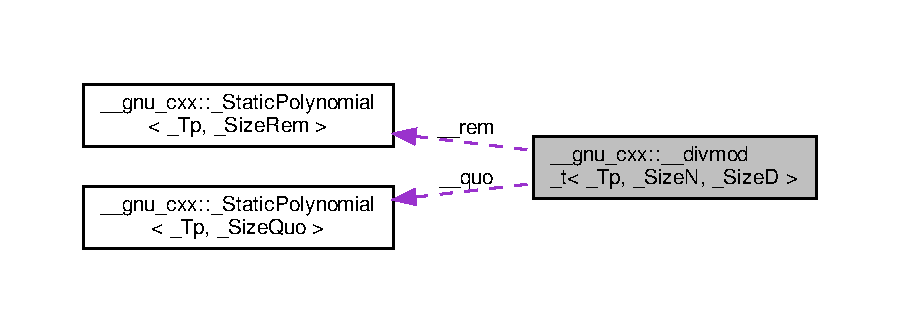
\includegraphics[width=350pt]{struct____gnu__cxx_1_1____divmod__t__coll__graph}
\end{center}
\end{figure}
\subsection*{Public Attributes}
\begin{DoxyCompactItemize}
\item 
\hyperlink{class____gnu__cxx_1_1__StaticPolynomial}{\+\_\+\+Static\+Polynomial}$<$ \+\_\+\+Tp, \hyperlink{struct____gnu__cxx_1_1____divmod__t_a813f65f5716a3d6b124020686b294a24}{\+\_\+\+Size\+Quo} $>$ \hyperlink{struct____gnu__cxx_1_1____divmod__t_a2d1cdc2ca4c92306d199cb1b70c1b7a2}{\+\_\+\+\_\+quo}
\item 
\hyperlink{class____gnu__cxx_1_1__StaticPolynomial}{\+\_\+\+Static\+Polynomial}$<$ \+\_\+\+Tp, \hyperlink{struct____gnu__cxx_1_1____divmod__t_a77870c1b7361b2b7511b0ef4d958826c}{\+\_\+\+Size\+Rem} $>$ \hyperlink{struct____gnu__cxx_1_1____divmod__t_ae3b5e6634fc53682a87e21d80fe44840}{\+\_\+\+\_\+rem}
\end{DoxyCompactItemize}
\subsection*{Static Public Attributes}
\begin{DoxyCompactItemize}
\item 
static constexpr std\+::size\+\_\+t \hyperlink{struct____gnu__cxx_1_1____divmod__t_a813f65f5716a3d6b124020686b294a24}{\+\_\+\+Size\+Quo} = (\+\_\+\+SizeD $<$= \+\_\+\+SizeN) ? \+\_\+\+SizeN -\/ \+\_\+\+SizeD + 1 \+: 1
\item 
static constexpr std\+::size\+\_\+t \hyperlink{struct____gnu__cxx_1_1____divmod__t_a77870c1b7361b2b7511b0ef4d958826c}{\+\_\+\+Size\+Rem} = (\+\_\+\+SizeD $>$ 1) ? \+\_\+\+SizeD -\/ 1 \+: 1
\end{DoxyCompactItemize}


\subsection{Detailed Description}
\subsubsection*{template$<$typename \+\_\+\+Tp, std\+::size\+\_\+t \+\_\+\+SizeN, std\+::size\+\_\+t \+\_\+\+SizeD$>$\newline
struct \+\_\+\+\_\+gnu\+\_\+cxx\+::\+\_\+\+\_\+divmod\+\_\+t$<$ \+\_\+\+Tp, \+\_\+\+Size\+N, \+\_\+\+Size\+D $>$}

Return type for divmod. 

Definition at line 783 of file static\+\_\+polynomial.\+h.



\subsection{Member Data Documentation}
\mbox{\Hypertarget{struct____gnu__cxx_1_1____divmod__t_a2d1cdc2ca4c92306d199cb1b70c1b7a2}\label{struct____gnu__cxx_1_1____divmod__t_a2d1cdc2ca4c92306d199cb1b70c1b7a2}} 
\index{\+\_\+\+\_\+gnu\+\_\+cxx\+::\+\_\+\+\_\+divmod\+\_\+t@{\+\_\+\+\_\+gnu\+\_\+cxx\+::\+\_\+\+\_\+divmod\+\_\+t}!\+\_\+\+\_\+quo@{\+\_\+\+\_\+quo}}
\index{\+\_\+\+\_\+quo@{\+\_\+\+\_\+quo}!\+\_\+\+\_\+gnu\+\_\+cxx\+::\+\_\+\+\_\+divmod\+\_\+t@{\+\_\+\+\_\+gnu\+\_\+cxx\+::\+\_\+\+\_\+divmod\+\_\+t}}
\subsubsection{\texorpdfstring{\+\_\+\+\_\+quo}{\_\_quo}}
{\footnotesize\ttfamily template$<$typename \+\_\+\+Tp , std\+::size\+\_\+t \+\_\+\+SizeN, std\+::size\+\_\+t \+\_\+\+SizeD$>$ \\
\hyperlink{class____gnu__cxx_1_1__StaticPolynomial}{\+\_\+\+Static\+Polynomial}$<$\+\_\+\+Tp, \hyperlink{struct____gnu__cxx_1_1____divmod__t_a813f65f5716a3d6b124020686b294a24}{\+\_\+\+Size\+Quo}$>$ \hyperlink{struct____gnu__cxx_1_1____divmod__t}{\+\_\+\+\_\+gnu\+\_\+cxx\+::\+\_\+\+\_\+divmod\+\_\+t}$<$ \+\_\+\+Tp, \+\_\+\+SizeN, \+\_\+\+SizeD $>$\+::\+\_\+\+\_\+quo}



Definition at line 790 of file static\+\_\+polynomial.\+h.

\mbox{\Hypertarget{struct____gnu__cxx_1_1____divmod__t_ae3b5e6634fc53682a87e21d80fe44840}\label{struct____gnu__cxx_1_1____divmod__t_ae3b5e6634fc53682a87e21d80fe44840}} 
\index{\+\_\+\+\_\+gnu\+\_\+cxx\+::\+\_\+\+\_\+divmod\+\_\+t@{\+\_\+\+\_\+gnu\+\_\+cxx\+::\+\_\+\+\_\+divmod\+\_\+t}!\+\_\+\+\_\+rem@{\+\_\+\+\_\+rem}}
\index{\+\_\+\+\_\+rem@{\+\_\+\+\_\+rem}!\+\_\+\+\_\+gnu\+\_\+cxx\+::\+\_\+\+\_\+divmod\+\_\+t@{\+\_\+\+\_\+gnu\+\_\+cxx\+::\+\_\+\+\_\+divmod\+\_\+t}}
\subsubsection{\texorpdfstring{\+\_\+\+\_\+rem}{\_\_rem}}
{\footnotesize\ttfamily template$<$typename \+\_\+\+Tp , std\+::size\+\_\+t \+\_\+\+SizeN, std\+::size\+\_\+t \+\_\+\+SizeD$>$ \\
\hyperlink{class____gnu__cxx_1_1__StaticPolynomial}{\+\_\+\+Static\+Polynomial}$<$\+\_\+\+Tp, \hyperlink{struct____gnu__cxx_1_1____divmod__t_a77870c1b7361b2b7511b0ef4d958826c}{\+\_\+\+Size\+Rem}$>$ \hyperlink{struct____gnu__cxx_1_1____divmod__t}{\+\_\+\+\_\+gnu\+\_\+cxx\+::\+\_\+\+\_\+divmod\+\_\+t}$<$ \+\_\+\+Tp, \+\_\+\+SizeN, \+\_\+\+SizeD $>$\+::\+\_\+\+\_\+rem}



Definition at line 791 of file static\+\_\+polynomial.\+h.

\mbox{\Hypertarget{struct____gnu__cxx_1_1____divmod__t_a813f65f5716a3d6b124020686b294a24}\label{struct____gnu__cxx_1_1____divmod__t_a813f65f5716a3d6b124020686b294a24}} 
\index{\+\_\+\+\_\+gnu\+\_\+cxx\+::\+\_\+\+\_\+divmod\+\_\+t@{\+\_\+\+\_\+gnu\+\_\+cxx\+::\+\_\+\+\_\+divmod\+\_\+t}!\+\_\+\+Size\+Quo@{\+\_\+\+Size\+Quo}}
\index{\+\_\+\+Size\+Quo@{\+\_\+\+Size\+Quo}!\+\_\+\+\_\+gnu\+\_\+cxx\+::\+\_\+\+\_\+divmod\+\_\+t@{\+\_\+\+\_\+gnu\+\_\+cxx\+::\+\_\+\+\_\+divmod\+\_\+t}}
\subsubsection{\texorpdfstring{\+\_\+\+Size\+Quo}{\_SizeQuo}}
{\footnotesize\ttfamily template$<$typename \+\_\+\+Tp , std\+::size\+\_\+t \+\_\+\+SizeN, std\+::size\+\_\+t \+\_\+\+SizeD$>$ \\
constexpr std\+::size\+\_\+t \hyperlink{struct____gnu__cxx_1_1____divmod__t}{\+\_\+\+\_\+gnu\+\_\+cxx\+::\+\_\+\+\_\+divmod\+\_\+t}$<$ \+\_\+\+Tp, \+\_\+\+SizeN, \+\_\+\+SizeD $>$\+::\+\_\+\+Size\+Quo = (\+\_\+\+SizeD $<$= \+\_\+\+SizeN) ? \+\_\+\+SizeN -\/ \+\_\+\+SizeD + 1 \+: 1\hspace{0.3cm}{\ttfamily [static]}}



Definition at line 786 of file static\+\_\+polynomial.\+h.

\mbox{\Hypertarget{struct____gnu__cxx_1_1____divmod__t_a77870c1b7361b2b7511b0ef4d958826c}\label{struct____gnu__cxx_1_1____divmod__t_a77870c1b7361b2b7511b0ef4d958826c}} 
\index{\+\_\+\+\_\+gnu\+\_\+cxx\+::\+\_\+\+\_\+divmod\+\_\+t@{\+\_\+\+\_\+gnu\+\_\+cxx\+::\+\_\+\+\_\+divmod\+\_\+t}!\+\_\+\+Size\+Rem@{\+\_\+\+Size\+Rem}}
\index{\+\_\+\+Size\+Rem@{\+\_\+\+Size\+Rem}!\+\_\+\+\_\+gnu\+\_\+cxx\+::\+\_\+\+\_\+divmod\+\_\+t@{\+\_\+\+\_\+gnu\+\_\+cxx\+::\+\_\+\+\_\+divmod\+\_\+t}}
\subsubsection{\texorpdfstring{\+\_\+\+Size\+Rem}{\_SizeRem}}
{\footnotesize\ttfamily template$<$typename \+\_\+\+Tp , std\+::size\+\_\+t \+\_\+\+SizeN, std\+::size\+\_\+t \+\_\+\+SizeD$>$ \\
constexpr std\+::size\+\_\+t \hyperlink{struct____gnu__cxx_1_1____divmod__t}{\+\_\+\+\_\+gnu\+\_\+cxx\+::\+\_\+\+\_\+divmod\+\_\+t}$<$ \+\_\+\+Tp, \+\_\+\+SizeN, \+\_\+\+SizeD $>$\+::\+\_\+\+Size\+Rem = (\+\_\+\+SizeD $>$ 1) ? \+\_\+\+SizeD -\/ 1 \+: 1\hspace{0.3cm}{\ttfamily [static]}}



Definition at line 788 of file static\+\_\+polynomial.\+h.



The documentation for this struct was generated from the following file\+:\begin{DoxyCompactItemize}
\item 
include/ext/\hyperlink{static__polynomial_8h}{static\+\_\+polynomial.\+h}\end{DoxyCompactItemize}

\hypertarget{struct____gnu__cxx_1_1____has__imag__t}{}\section{\+\_\+\+\_\+gnu\+\_\+cxx\+:\+:\+\_\+\+\_\+has\+\_\+imag\+\_\+t$<$ typename, typename $>$ Struct Template Reference}
\label{struct____gnu__cxx_1_1____has__imag__t}\index{\+\_\+\+\_\+gnu\+\_\+cxx\+::\+\_\+\+\_\+has\+\_\+imag\+\_\+t$<$ typename, typename $>$@{\+\_\+\+\_\+gnu\+\_\+cxx\+::\+\_\+\+\_\+has\+\_\+imag\+\_\+t$<$ typename, typename $>$}}


{\ttfamily \#include $<$polynomial.\+h$>$}



Inheritance diagram for \+\_\+\+\_\+gnu\+\_\+cxx\+:\+:\+\_\+\+\_\+has\+\_\+imag\+\_\+t$<$ typename, typename $>$\+:
\nopagebreak
\begin{figure}[H]
\begin{center}
\leavevmode
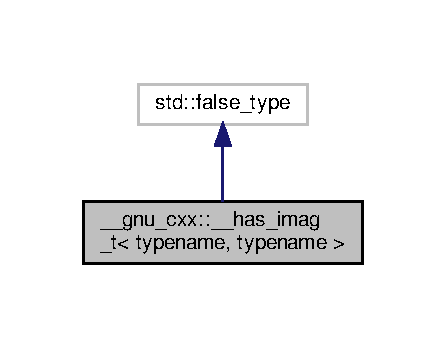
\includegraphics[width=214pt]{struct____gnu__cxx_1_1____has__imag__t__inherit__graph}
\end{center}
\end{figure}


Collaboration diagram for \+\_\+\+\_\+gnu\+\_\+cxx\+:\+:\+\_\+\+\_\+has\+\_\+imag\+\_\+t$<$ typename, typename $>$\+:
\nopagebreak
\begin{figure}[H]
\begin{center}
\leavevmode
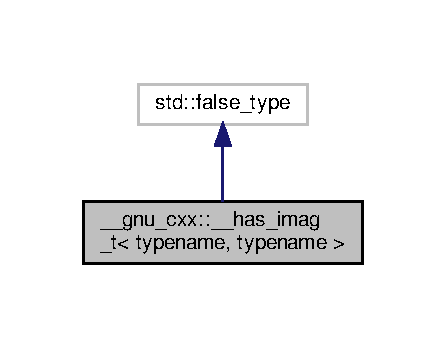
\includegraphics[width=214pt]{struct____gnu__cxx_1_1____has__imag__t__coll__graph}
\end{center}
\end{figure}


\subsection{Detailed Description}
\subsubsection*{template$<$typename, typename = std\+::void\+\_\+t$<$$>$$>$\newline
struct \+\_\+\+\_\+gnu\+\_\+cxx\+::\+\_\+\+\_\+has\+\_\+imag\+\_\+t$<$ typename, typename $>$}



Definition at line 102 of file polynomial.\+h.



The documentation for this struct was generated from the following file\+:\begin{DoxyCompactItemize}
\item 
include/ext/\hyperlink{polynomial_8h}{polynomial.\+h}\end{DoxyCompactItemize}

\hypertarget{struct____gnu__cxx_1_1____has__imag__t_3_01__Tp_00_01std_1_1void__t_3_01decltype_07std_1_1declva705d5f96db36a5134d7de4531d29483c}{}\section{\+\_\+\+\_\+gnu\+\_\+cxx\+:\+:\+\_\+\+\_\+has\+\_\+imag\+\_\+t$<$ \+\_\+\+Tp, std\+:\+:void\+\_\+t$<$ decltype(std\+:\+:declval$<$ \+\_\+\+Tp \& $>$().imag())$>$ $>$ Struct Template Reference}
\label{struct____gnu__cxx_1_1____has__imag__t_3_01__Tp_00_01std_1_1void__t_3_01decltype_07std_1_1declva705d5f96db36a5134d7de4531d29483c}\index{\+\_\+\+\_\+gnu\+\_\+cxx\+::\+\_\+\+\_\+has\+\_\+imag\+\_\+t$<$ \+\_\+\+Tp, std\+::void\+\_\+t$<$ decltype(std\+::declval$<$ \+\_\+\+Tp \& $>$().\+imag())$>$ $>$@{\+\_\+\+\_\+gnu\+\_\+cxx\+::\+\_\+\+\_\+has\+\_\+imag\+\_\+t$<$ \+\_\+\+Tp, std\+::void\+\_\+t$<$ decltype(std\+::declval$<$ \+\_\+\+Tp \& $>$().\+imag())$>$ $>$}}


{\ttfamily \#include $<$polynomial.\+h$>$}



Inheritance diagram for \+\_\+\+\_\+gnu\+\_\+cxx\+:\+:\+\_\+\+\_\+has\+\_\+imag\+\_\+t$<$ \+\_\+\+Tp, std\+:\+:void\+\_\+t$<$ decltype(std\+:\+:declval$<$ \+\_\+\+Tp \& $>$().imag())$>$ $>$\+:
\nopagebreak
\begin{figure}[H]
\begin{center}
\leavevmode
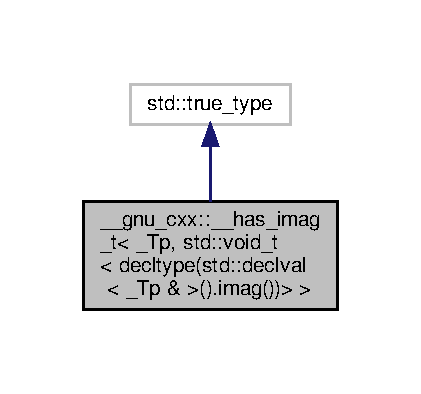
\includegraphics[width=202pt]{struct____gnu__cxx_1_1____has__imag__t_3_01__Tp_00_01std_1_1void__t_3_01decltype_07std_1_1declva57d94c7c383c14ae9cda8a5fc631a69e}
\end{center}
\end{figure}


Collaboration diagram for \+\_\+\+\_\+gnu\+\_\+cxx\+:\+:\+\_\+\+\_\+has\+\_\+imag\+\_\+t$<$ \+\_\+\+Tp, std\+:\+:void\+\_\+t$<$ decltype(std\+:\+:declval$<$ \+\_\+\+Tp \& $>$().imag())$>$ $>$\+:
\nopagebreak
\begin{figure}[H]
\begin{center}
\leavevmode
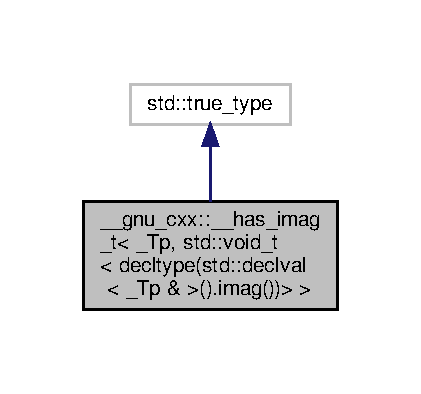
\includegraphics[width=202pt]{struct____gnu__cxx_1_1____has__imag__t_3_01__Tp_00_01std_1_1void__t_3_01decltype_07std_1_1declva76c1ac43224ce0c47cb3099336023b94}
\end{center}
\end{figure}


\subsection{Detailed Description}
\subsubsection*{template$<$typename \+\_\+\+Tp$>$\newline
struct \+\_\+\+\_\+gnu\+\_\+cxx\+::\+\_\+\+\_\+has\+\_\+imag\+\_\+t$<$ \+\_\+\+Tp, std\+::void\+\_\+t$<$ decltype(std\+::declval$<$ \+\_\+\+Tp \& $>$().\+imag())$>$ $>$}



Definition at line 107 of file polynomial.\+h.



The documentation for this struct was generated from the following file\+:\begin{DoxyCompactItemize}
\item 
include/ext/\hyperlink{polynomial_8h}{polynomial.\+h}\end{DoxyCompactItemize}

\hypertarget{struct____gnu__cxx_1_1____has__value__type__t}{}\section{\+\_\+\+\_\+gnu\+\_\+cxx\+:\+:\+\_\+\+\_\+has\+\_\+value\+\_\+type\+\_\+t$<$ typename, typename $>$ Struct Template Reference}
\label{struct____gnu__cxx_1_1____has__value__type__t}\index{\+\_\+\+\_\+gnu\+\_\+cxx\+::\+\_\+\+\_\+has\+\_\+value\+\_\+type\+\_\+t$<$ typename, typename $>$@{\+\_\+\+\_\+gnu\+\_\+cxx\+::\+\_\+\+\_\+has\+\_\+value\+\_\+type\+\_\+t$<$ typename, typename $>$}}


{\ttfamily \#include $<$polynomial.\+h$>$}



Inheritance diagram for \+\_\+\+\_\+gnu\+\_\+cxx\+:\+:\+\_\+\+\_\+has\+\_\+value\+\_\+type\+\_\+t$<$ typename, typename $>$\+:
\nopagebreak
\begin{figure}[H]
\begin{center}
\leavevmode
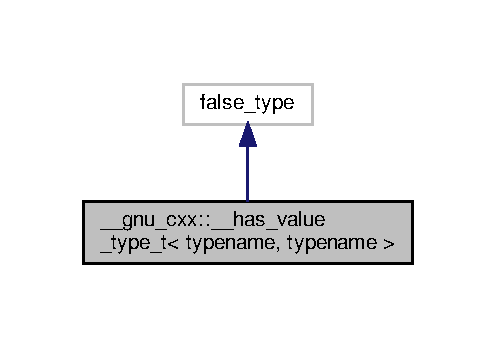
\includegraphics[width=238pt]{struct____gnu__cxx_1_1____has__value__type__t__inherit__graph}
\end{center}
\end{figure}


Collaboration diagram for \+\_\+\+\_\+gnu\+\_\+cxx\+:\+:\+\_\+\+\_\+has\+\_\+value\+\_\+type\+\_\+t$<$ typename, typename $>$\+:
\nopagebreak
\begin{figure}[H]
\begin{center}
\leavevmode
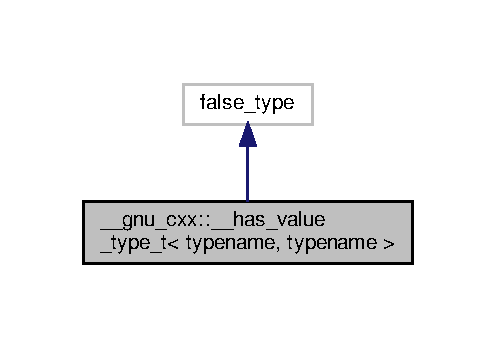
\includegraphics[width=238pt]{struct____gnu__cxx_1_1____has__value__type__t__coll__graph}
\end{center}
\end{figure}


\subsection{Detailed Description}
\subsubsection*{template$<$typename, typename = std\+::void\+\_\+t$<$$>$$>$\newline
struct \+\_\+\+\_\+gnu\+\_\+cxx\+::\+\_\+\+\_\+has\+\_\+value\+\_\+type\+\_\+t$<$ typename, typename $>$}



Definition at line 116 of file polynomial.\+h.



The documentation for this struct was generated from the following file\+:\begin{DoxyCompactItemize}
\item 
include/ext/\hyperlink{polynomial_8h}{polynomial.\+h}\end{DoxyCompactItemize}

\hypertarget{struct____gnu__cxx_1_1____has__value__type__t_3_01__Tp_00_01std_1_1void__t_3_01typename_01__Tp_1_1value__type_01_4_01_4}{}\section{\+\_\+\+\_\+gnu\+\_\+cxx\+:\+:\+\_\+\+\_\+has\+\_\+value\+\_\+type\+\_\+t$<$ \+\_\+\+Tp, std\+:\+:void\+\_\+t$<$ typename \+\_\+\+Tp\+:\+:value\+\_\+type $>$ $>$ Struct Template Reference}
\label{struct____gnu__cxx_1_1____has__value__type__t_3_01__Tp_00_01std_1_1void__t_3_01typename_01__Tp_1_1value__type_01_4_01_4}\index{\+\_\+\+\_\+gnu\+\_\+cxx\+::\+\_\+\+\_\+has\+\_\+value\+\_\+type\+\_\+t$<$ \+\_\+\+Tp, std\+::void\+\_\+t$<$ typename \+\_\+\+Tp\+::value\+\_\+type $>$ $>$@{\+\_\+\+\_\+gnu\+\_\+cxx\+::\+\_\+\+\_\+has\+\_\+value\+\_\+type\+\_\+t$<$ \+\_\+\+Tp, std\+::void\+\_\+t$<$ typename \+\_\+\+Tp\+::value\+\_\+type $>$ $>$}}


{\ttfamily \#include $<$polynomial.\+h$>$}



Inheritance diagram for \+\_\+\+\_\+gnu\+\_\+cxx\+:\+:\+\_\+\+\_\+has\+\_\+value\+\_\+type\+\_\+t$<$ \+\_\+\+Tp, std\+:\+:void\+\_\+t$<$ typename \+\_\+\+Tp\+:\+:value\+\_\+type $>$ $>$\+:
\nopagebreak
\begin{figure}[H]
\begin{center}
\leavevmode
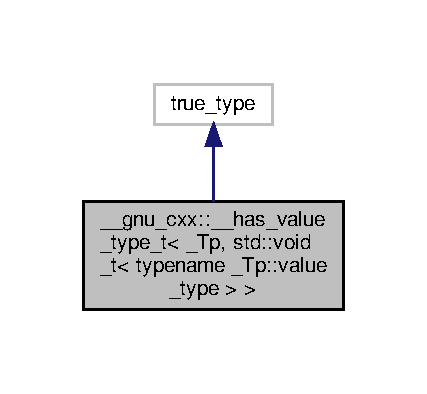
\includegraphics[width=205pt]{struct____gnu__cxx_1_1____has__value__type__t_3_01__Tp_00_01std_1_1void__t_3_01typename_01__Tp_1dc53b51a0e8d38321c66760e53731ac5}
\end{center}
\end{figure}


Collaboration diagram for \+\_\+\+\_\+gnu\+\_\+cxx\+:\+:\+\_\+\+\_\+has\+\_\+value\+\_\+type\+\_\+t$<$ \+\_\+\+Tp, std\+:\+:void\+\_\+t$<$ typename \+\_\+\+Tp\+:\+:value\+\_\+type $>$ $>$\+:
\nopagebreak
\begin{figure}[H]
\begin{center}
\leavevmode
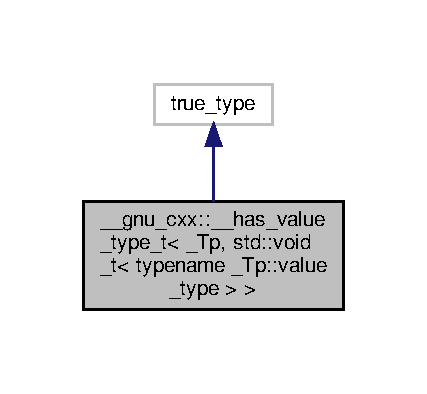
\includegraphics[width=205pt]{struct____gnu__cxx_1_1____has__value__type__t_3_01__Tp_00_01std_1_1void__t_3_01typename_01__Tp_19b6b1d0c9a4175ab39384b4519116c9f}
\end{center}
\end{figure}


\subsection{Detailed Description}
\subsubsection*{template$<$typename \+\_\+\+Tp$>$\newline
struct \+\_\+\+\_\+gnu\+\_\+cxx\+::\+\_\+\+\_\+has\+\_\+value\+\_\+type\+\_\+t$<$ \+\_\+\+Tp, std\+::void\+\_\+t$<$ typename \+\_\+\+Tp\+::value\+\_\+type $>$ $>$}



Definition at line 121 of file polynomial.\+h.



The documentation for this struct was generated from the following file\+:\begin{DoxyCompactItemize}
\item 
include/ext/\hyperlink{polynomial_8h}{polynomial.\+h}\end{DoxyCompactItemize}

\hypertarget{struct____gnu__cxx_1_1____real__type}{}\section{\+\_\+\+\_\+gnu\+\_\+cxx\+:\+:\+\_\+\+\_\+real\+\_\+type$<$ \+\_\+\+Tp $>$ Struct Template Reference}
\label{struct____gnu__cxx_1_1____real__type}\index{\+\_\+\+\_\+gnu\+\_\+cxx\+::\+\_\+\+\_\+real\+\_\+type$<$ \+\_\+\+Tp $>$@{\+\_\+\+\_\+gnu\+\_\+cxx\+::\+\_\+\+\_\+real\+\_\+type$<$ \+\_\+\+Tp $>$}}


{\ttfamily \#include $<$polynomial.\+h$>$}

\subsection*{Public Types}
\begin{DoxyCompactItemize}
\item 
using \hyperlink{struct____gnu__cxx_1_1____real__type_a39bc08f342aaa6ef7e02c6711c611b74}{type} = \+\_\+\+Tp
\end{DoxyCompactItemize}


\subsection{Detailed Description}
\subsubsection*{template$<$typename \+\_\+\+Tp$>$\newline
struct \+\_\+\+\_\+gnu\+\_\+cxx\+::\+\_\+\+\_\+real\+\_\+type$<$ \+\_\+\+Tp $>$}



Definition at line 133 of file polynomial.\+h.



\subsection{Member Typedef Documentation}
\mbox{\Hypertarget{struct____gnu__cxx_1_1____real__type_a39bc08f342aaa6ef7e02c6711c611b74}\label{struct____gnu__cxx_1_1____real__type_a39bc08f342aaa6ef7e02c6711c611b74}} 
\index{\+\_\+\+\_\+gnu\+\_\+cxx\+::\+\_\+\+\_\+real\+\_\+type@{\+\_\+\+\_\+gnu\+\_\+cxx\+::\+\_\+\+\_\+real\+\_\+type}!type@{type}}
\index{type@{type}!\+\_\+\+\_\+gnu\+\_\+cxx\+::\+\_\+\+\_\+real\+\_\+type@{\+\_\+\+\_\+gnu\+\_\+cxx\+::\+\_\+\+\_\+real\+\_\+type}}
\subsubsection{\texorpdfstring{type}{type}}
{\footnotesize\ttfamily template$<$typename \+\_\+\+Tp$>$ \\
using \hyperlink{struct____gnu__cxx_1_1____real__type}{\+\_\+\+\_\+gnu\+\_\+cxx\+::\+\_\+\+\_\+real\+\_\+type}$<$ \+\_\+\+Tp $>$\+::\hyperlink{struct____gnu__cxx_1_1____real__type_a39bc08f342aaa6ef7e02c6711c611b74}{type} =  \+\_\+\+Tp}



Definition at line 134 of file polynomial.\+h.



The documentation for this struct was generated from the following file\+:\begin{DoxyCompactItemize}
\item 
include/ext/\hyperlink{polynomial_8h}{polynomial.\+h}\end{DoxyCompactItemize}

\hypertarget{struct____gnu__cxx_1_1____real__type_3_01__Polynomial_3_01__Tp_01_4_01_4}{}\section{\+\_\+\+\_\+gnu\+\_\+cxx\+:\+:\+\_\+\+\_\+real\+\_\+type$<$ \+\_\+\+Polynomial$<$ \+\_\+\+Tp $>$ $>$ Struct Template Reference}
\label{struct____gnu__cxx_1_1____real__type_3_01__Polynomial_3_01__Tp_01_4_01_4}\index{\+\_\+\+\_\+gnu\+\_\+cxx\+::\+\_\+\+\_\+real\+\_\+type$<$ \+\_\+\+Polynomial$<$ \+\_\+\+Tp $>$ $>$@{\+\_\+\+\_\+gnu\+\_\+cxx\+::\+\_\+\+\_\+real\+\_\+type$<$ \+\_\+\+Polynomial$<$ \+\_\+\+Tp $>$ $>$}}


{\ttfamily \#include $<$polynomial.\+h$>$}

\subsection*{Public Types}
\begin{DoxyCompactItemize}
\item 
using \hyperlink{struct____gnu__cxx_1_1____real__type_3_01__Polynomial_3_01__Tp_01_4_01_4_ac0fd9a1c448f5e710c2df57e1c3a3f54}{type} = typename \hyperlink{class____gnu__cxx_1_1__Polynomial}{\+\_\+\+Polynomial}$<$ \+\_\+\+Tp $>$\+::real\+\_\+type
\end{DoxyCompactItemize}


\subsection{Detailed Description}
\subsubsection*{template$<$typename \+\_\+\+Tp$>$\newline
struct \+\_\+\+\_\+gnu\+\_\+cxx\+::\+\_\+\+\_\+real\+\_\+type$<$ \+\_\+\+Polynomial$<$ \+\_\+\+Tp $>$ $>$}



Definition at line 840 of file polynomial.\+h.



\subsection{Member Typedef Documentation}
\mbox{\Hypertarget{struct____gnu__cxx_1_1____real__type_3_01__Polynomial_3_01__Tp_01_4_01_4_ac0fd9a1c448f5e710c2df57e1c3a3f54}\label{struct____gnu__cxx_1_1____real__type_3_01__Polynomial_3_01__Tp_01_4_01_4_ac0fd9a1c448f5e710c2df57e1c3a3f54}} 
\index{\+\_\+\+\_\+gnu\+\_\+cxx\+::\+\_\+\+\_\+real\+\_\+type$<$ \+\_\+\+Polynomial$<$ \+\_\+\+Tp $>$ $>$@{\+\_\+\+\_\+gnu\+\_\+cxx\+::\+\_\+\+\_\+real\+\_\+type$<$ \+\_\+\+Polynomial$<$ \+\_\+\+Tp $>$ $>$}!type@{type}}
\index{type@{type}!\+\_\+\+\_\+gnu\+\_\+cxx\+::\+\_\+\+\_\+real\+\_\+type$<$ \+\_\+\+Polynomial$<$ \+\_\+\+Tp $>$ $>$@{\+\_\+\+\_\+gnu\+\_\+cxx\+::\+\_\+\+\_\+real\+\_\+type$<$ \+\_\+\+Polynomial$<$ \+\_\+\+Tp $>$ $>$}}
\subsubsection{\texorpdfstring{type}{type}}
{\footnotesize\ttfamily template$<$typename \+\_\+\+Tp $>$ \\
using \hyperlink{struct____gnu__cxx_1_1____real__type}{\+\_\+\+\_\+gnu\+\_\+cxx\+::\+\_\+\+\_\+real\+\_\+type}$<$ \hyperlink{class____gnu__cxx_1_1__Polynomial}{\+\_\+\+Polynomial}$<$ \+\_\+\+Tp $>$ $>$\+::\hyperlink{struct____gnu__cxx_1_1____real__type_3_01__Polynomial_3_01__Tp_01_4_01_4_ac0fd9a1c448f5e710c2df57e1c3a3f54}{type} =  typename \hyperlink{class____gnu__cxx_1_1__Polynomial}{\+\_\+\+Polynomial}$<$\+\_\+\+Tp$>$\+::real\+\_\+type}



Definition at line 841 of file polynomial.\+h.



The documentation for this struct was generated from the following file\+:\begin{DoxyCompactItemize}
\item 
include/ext/\hyperlink{polynomial_8h}{polynomial.\+h}\end{DoxyCompactItemize}

\hypertarget{struct____gnu__cxx_1_1____real__type_3_01std_1_1complex_3_01__Tp_01_4_01_4}{}\section{\+\_\+\+\_\+gnu\+\_\+cxx\+:\+:\+\_\+\+\_\+real\+\_\+type$<$ std\+:\+:complex$<$ \+\_\+\+Tp $>$ $>$ Struct Template Reference}
\label{struct____gnu__cxx_1_1____real__type_3_01std_1_1complex_3_01__Tp_01_4_01_4}\index{\+\_\+\+\_\+gnu\+\_\+cxx\+::\+\_\+\+\_\+real\+\_\+type$<$ std\+::complex$<$ \+\_\+\+Tp $>$ $>$@{\+\_\+\+\_\+gnu\+\_\+cxx\+::\+\_\+\+\_\+real\+\_\+type$<$ std\+::complex$<$ \+\_\+\+Tp $>$ $>$}}


{\ttfamily \#include $<$polynomial.\+h$>$}

\subsection*{Public Types}
\begin{DoxyCompactItemize}
\item 
using \hyperlink{struct____gnu__cxx_1_1____real__type_3_01std_1_1complex_3_01__Tp_01_4_01_4_a038d9970ff97c1b3eeb53f5eb08fdfe1}{type} = \+\_\+\+Tp
\end{DoxyCompactItemize}


\subsection{Detailed Description}
\subsubsection*{template$<$typename \+\_\+\+Tp$>$\newline
struct \+\_\+\+\_\+gnu\+\_\+cxx\+::\+\_\+\+\_\+real\+\_\+type$<$ std\+::complex$<$ \+\_\+\+Tp $>$ $>$}



Definition at line 137 of file polynomial.\+h.



\subsection{Member Typedef Documentation}
\mbox{\Hypertarget{struct____gnu__cxx_1_1____real__type_3_01std_1_1complex_3_01__Tp_01_4_01_4_a038d9970ff97c1b3eeb53f5eb08fdfe1}\label{struct____gnu__cxx_1_1____real__type_3_01std_1_1complex_3_01__Tp_01_4_01_4_a038d9970ff97c1b3eeb53f5eb08fdfe1}} 
\index{\+\_\+\+\_\+gnu\+\_\+cxx\+::\+\_\+\+\_\+real\+\_\+type$<$ std\+::complex$<$ \+\_\+\+Tp $>$ $>$@{\+\_\+\+\_\+gnu\+\_\+cxx\+::\+\_\+\+\_\+real\+\_\+type$<$ std\+::complex$<$ \+\_\+\+Tp $>$ $>$}!type@{type}}
\index{type@{type}!\+\_\+\+\_\+gnu\+\_\+cxx\+::\+\_\+\+\_\+real\+\_\+type$<$ std\+::complex$<$ \+\_\+\+Tp $>$ $>$@{\+\_\+\+\_\+gnu\+\_\+cxx\+::\+\_\+\+\_\+real\+\_\+type$<$ std\+::complex$<$ \+\_\+\+Tp $>$ $>$}}
\subsubsection{\texorpdfstring{type}{type}}
{\footnotesize\ttfamily template$<$typename \+\_\+\+Tp $>$ \\
using \hyperlink{struct____gnu__cxx_1_1____real__type}{\+\_\+\+\_\+gnu\+\_\+cxx\+::\+\_\+\+\_\+real\+\_\+type}$<$ std\+::complex$<$ \+\_\+\+Tp $>$ $>$\+::\hyperlink{struct____gnu__cxx_1_1____real__type_3_01std_1_1complex_3_01__Tp_01_4_01_4_a038d9970ff97c1b3eeb53f5eb08fdfe1}{type} =  \+\_\+\+Tp}



Definition at line 138 of file polynomial.\+h.



The documentation for this struct was generated from the following file\+:\begin{DoxyCompactItemize}
\item 
include/ext/\hyperlink{polynomial_8h}{polynomial.\+h}\end{DoxyCompactItemize}

\hypertarget{class____gnu__cxx_1_1__Polynomial}{}\section{\+\_\+\+\_\+gnu\+\_\+cxx\+:\+:\+\_\+\+Polynomial$<$ \+\_\+\+Tp $>$ Class Template Reference}
\label{class____gnu__cxx_1_1__Polynomial}\index{\+\_\+\+\_\+gnu\+\_\+cxx\+::\+\_\+\+Polynomial$<$ \+\_\+\+Tp $>$@{\+\_\+\+\_\+gnu\+\_\+cxx\+::\+\_\+\+Polynomial$<$ \+\_\+\+Tp $>$}}


A dense polynomial class with a contiguous array of coefficients. The coefficients are lowest-\/order first\+: \[ P(x) = a_0 + a_1 x + ... + a_n x^n \].  




{\ttfamily \#include $<$polynomial.\+h$>$}

\subsection*{Public Types}
\begin{DoxyCompactItemize}
\item 
using \hyperlink{class____gnu__cxx_1_1__Polynomial_a96e4523cc2a834724fe4224f0800486b}{const\+\_\+iterator} = typename std\+::vector$<$ \hyperlink{class____gnu__cxx_1_1__Polynomial_a725563351f50e76084a7a016c06f8a53}{value\+\_\+type} $>$\+::\hyperlink{class____gnu__cxx_1_1__Polynomial_a96e4523cc2a834724fe4224f0800486b}{const\+\_\+iterator}
\item 
using \hyperlink{class____gnu__cxx_1_1__Polynomial_aaf4c4bbd516b837df5fe70b3bda4e9af}{const\+\_\+pointer} = typename std\+::vector$<$ \hyperlink{class____gnu__cxx_1_1__Polynomial_a725563351f50e76084a7a016c06f8a53}{value\+\_\+type} $>$\+::\hyperlink{class____gnu__cxx_1_1__Polynomial_aaf4c4bbd516b837df5fe70b3bda4e9af}{const\+\_\+pointer}
\item 
using \hyperlink{class____gnu__cxx_1_1__Polynomial_a55e17774f3387e74adb57376d099cf16}{const\+\_\+reference} = typename std\+::vector$<$ \hyperlink{class____gnu__cxx_1_1__Polynomial_a725563351f50e76084a7a016c06f8a53}{value\+\_\+type} $>$\+::\hyperlink{class____gnu__cxx_1_1__Polynomial_a55e17774f3387e74adb57376d099cf16}{const\+\_\+reference}
\item 
using \hyperlink{class____gnu__cxx_1_1__Polynomial_a2a042a80127ab9a7b0349a54791e59af}{const\+\_\+reverse\+\_\+iterator} = typename std\+::vector$<$ \hyperlink{class____gnu__cxx_1_1__Polynomial_a725563351f50e76084a7a016c06f8a53}{value\+\_\+type} $>$\+::\hyperlink{class____gnu__cxx_1_1__Polynomial_a2a042a80127ab9a7b0349a54791e59af}{const\+\_\+reverse\+\_\+iterator}
\item 
using \hyperlink{class____gnu__cxx_1_1__Polynomial_a1b1f56c1951282267a0d18a420f53b80}{difference\+\_\+type} = typename std\+::vector$<$ \hyperlink{class____gnu__cxx_1_1__Polynomial_a725563351f50e76084a7a016c06f8a53}{value\+\_\+type} $>$\+::\hyperlink{class____gnu__cxx_1_1__Polynomial_a1b1f56c1951282267a0d18a420f53b80}{difference\+\_\+type}
\item 
using \hyperlink{class____gnu__cxx_1_1__Polynomial_a64bd557b6af46992e352dbe9e30fa201}{iterator} = typename std\+::vector$<$ \hyperlink{class____gnu__cxx_1_1__Polynomial_a725563351f50e76084a7a016c06f8a53}{value\+\_\+type} $>$\+::\hyperlink{class____gnu__cxx_1_1__Polynomial_a64bd557b6af46992e352dbe9e30fa201}{iterator}
\item 
using \hyperlink{class____gnu__cxx_1_1__Polynomial_a876dcb9c1b92c4896a3f3b9f26e7e3df}{pointer} = typename std\+::vector$<$ \hyperlink{class____gnu__cxx_1_1__Polynomial_a725563351f50e76084a7a016c06f8a53}{value\+\_\+type} $>$\+::\hyperlink{class____gnu__cxx_1_1__Polynomial_a876dcb9c1b92c4896a3f3b9f26e7e3df}{pointer}
\item 
using \hyperlink{class____gnu__cxx_1_1__Polynomial_a656ceaafcb42abd626c253da3284998b}{real\+\_\+type} = \hyperlink{namespace____gnu__cxx_a3f707c0c6f6926cf68b74072733751f7}{\+\_\+\+\_\+real\+\_\+type\+\_\+t}$<$ \+\_\+\+Tp $>$
\item 
using \hyperlink{class____gnu__cxx_1_1__Polynomial_accb3b4df60e4ad82d466173d54ea731a}{reference} = typename std\+::vector$<$ \hyperlink{class____gnu__cxx_1_1__Polynomial_a725563351f50e76084a7a016c06f8a53}{value\+\_\+type} $>$\+::\hyperlink{class____gnu__cxx_1_1__Polynomial_accb3b4df60e4ad82d466173d54ea731a}{reference}
\item 
using \hyperlink{class____gnu__cxx_1_1__Polynomial_aed8f7d97c575d5c34c54170631953415}{reverse\+\_\+iterator} = typename std\+::vector$<$ \hyperlink{class____gnu__cxx_1_1__Polynomial_a725563351f50e76084a7a016c06f8a53}{value\+\_\+type} $>$\+::\hyperlink{class____gnu__cxx_1_1__Polynomial_aed8f7d97c575d5c34c54170631953415}{reverse\+\_\+iterator}
\item 
using \hyperlink{class____gnu__cxx_1_1__Polynomial_a8b25fcfd4acaad0c5c08b649c22da28a}{size\+\_\+type} = typename std\+::vector$<$ \hyperlink{class____gnu__cxx_1_1__Polynomial_a725563351f50e76084a7a016c06f8a53}{value\+\_\+type} $>$\+::\hyperlink{class____gnu__cxx_1_1__Polynomial_a8b25fcfd4acaad0c5c08b649c22da28a}{size\+\_\+type}
\item 
using \hyperlink{class____gnu__cxx_1_1__Polynomial_a725563351f50e76084a7a016c06f8a53}{value\+\_\+type} = typename std\+::vector$<$ \+\_\+\+Tp $>$\+::\hyperlink{class____gnu__cxx_1_1__Polynomial_a725563351f50e76084a7a016c06f8a53}{value\+\_\+type}
\end{DoxyCompactItemize}
\subsection*{Public Member Functions}
\begin{DoxyCompactItemize}
\item 
\hyperlink{class____gnu__cxx_1_1__Polynomial_ad2baf4c12b7e3ab131a592afa3f391ae}{\+\_\+\+Polynomial} ()
\item 
\hyperlink{class____gnu__cxx_1_1__Polynomial_ac0a657bc804f3db8a03acfd1b98abb39}{\+\_\+\+Polynomial} (const \hyperlink{class____gnu__cxx_1_1__Polynomial}{\+\_\+\+Polynomial} \&)=default
\item 
\hyperlink{class____gnu__cxx_1_1__Polynomial_a87bad90934c9752b51cdece15a5b369f}{\+\_\+\+Polynomial} (\hyperlink{class____gnu__cxx_1_1__Polynomial}{\+\_\+\+Polynomial} \&\&) noexcept=default
\item 
{\footnotesize template$<$typename \+\_\+\+Up $>$ }\\\hyperlink{class____gnu__cxx_1_1__Polynomial_ae744374b972b91a9609ba6cc1330bbfd}{\+\_\+\+Polynomial} (const \hyperlink{class____gnu__cxx_1_1__Polynomial}{\+\_\+\+Polynomial}$<$ \hyperlink{class____gnu__cxx_1_1__Polynomial_a242114d4b86648a5dff67a8221f80d40}{\+\_\+\+Up} $>$ \&\+\_\+\+\_\+poly)
\item 
\hyperlink{class____gnu__cxx_1_1__Polynomial_ad89b416fedd4e3a23b484d5269767a93}{\+\_\+\+Polynomial} (\hyperlink{class____gnu__cxx_1_1__Polynomial_a725563351f50e76084a7a016c06f8a53}{value\+\_\+type} \+\_\+\+\_\+a, \hyperlink{class____gnu__cxx_1_1__Polynomial_a8b25fcfd4acaad0c5c08b649c22da28a}{size\+\_\+type} \+\_\+\+\_\+degree=0)
\item 
\hyperlink{class____gnu__cxx_1_1__Polynomial_acc6b7b2a52600f62bf8dee99f2fb787c}{\+\_\+\+Polynomial} (std\+::initializer\+\_\+list$<$ \hyperlink{class____gnu__cxx_1_1__Polynomial_a725563351f50e76084a7a016c06f8a53}{value\+\_\+type} $>$ \+\_\+\+\_\+ila)
\item 
{\footnotesize template$<$typename In\+Iter , typename  = std\+::\+\_\+\+Require\+Input\+Iter$<$\+In\+Iter$>$$>$ }\\\hyperlink{class____gnu__cxx_1_1__Polynomial_a45589d1d036861179488c44f3029f335}{\+\_\+\+Polynomial} (const In\+Iter \&\+\_\+\+\_\+abegin, const In\+Iter \&\+\_\+\+\_\+aend)
\item 
{\footnotesize template$<$typename In\+Iter , typename  = std\+::\+\_\+\+Require\+Input\+Iter$<$\+In\+Iter$>$$>$ }\\\hyperlink{class____gnu__cxx_1_1__Polynomial_a86249f53e97e72eff11242a8ba85ba4c}{\+\_\+\+Polynomial} (const In\+Iter \&\+\_\+\+\_\+xbegin, const In\+Iter \&\+\_\+\+\_\+xend, const In\+Iter \&\+\_\+\+\_\+ybegin)
\item 
{\footnotesize template$<$typename Gen $>$ }\\\hyperlink{class____gnu__cxx_1_1__Polynomial_ad6e0daed9aa3a89cd98441a0fc4fa9f1}{\+\_\+\+Polynomial} (Gen \+\_\+\+\_\+gen, \hyperlink{class____gnu__cxx_1_1__Polynomial_a8b25fcfd4acaad0c5c08b649c22da28a}{size\+\_\+type} \+\_\+\+\_\+degree)
\item 
\hyperlink{class____gnu__cxx_1_1__Polynomial_a64bd557b6af46992e352dbe9e30fa201}{iterator} \hyperlink{class____gnu__cxx_1_1__Polynomial_a2f9cf484724c2aef472975fc3d8bd99d}{begin} () noexcept
\item 
\hyperlink{class____gnu__cxx_1_1__Polynomial_a96e4523cc2a834724fe4224f0800486b}{const\+\_\+iterator} \hyperlink{class____gnu__cxx_1_1__Polynomial_a57902287656245f5ae1ee7406b419c9b}{begin} () const noexcept
\item 
\hyperlink{class____gnu__cxx_1_1__Polynomial_a96e4523cc2a834724fe4224f0800486b}{const\+\_\+iterator} \hyperlink{class____gnu__cxx_1_1__Polynomial_a3309265141727a7581036a2b7632c689}{cbegin} () const noexcept
\item 
\hyperlink{class____gnu__cxx_1_1__Polynomial_a96e4523cc2a834724fe4224f0800486b}{const\+\_\+iterator} \hyperlink{class____gnu__cxx_1_1__Polynomial_ae3d5b393866c55f9585a1e0e10c41cc4}{cend} () const noexcept
\item 
\hyperlink{class____gnu__cxx_1_1__Polynomial_a725563351f50e76084a7a016c06f8a53}{value\+\_\+type} \hyperlink{class____gnu__cxx_1_1__Polynomial_a7cee31b3acbe8c024af6d696bc610f49}{coefficient} (\hyperlink{class____gnu__cxx_1_1__Polynomial_a8b25fcfd4acaad0c5c08b649c22da28a}{size\+\_\+type} \+\_\+\+\_\+i) const
\item 
void \hyperlink{class____gnu__cxx_1_1__Polynomial_a191611909a0461c449984a0898bce38f}{coefficient} (\hyperlink{class____gnu__cxx_1_1__Polynomial_a8b25fcfd4acaad0c5c08b649c22da28a}{size\+\_\+type} \+\_\+\+\_\+i, \hyperlink{class____gnu__cxx_1_1__Polynomial_a725563351f50e76084a7a016c06f8a53}{value\+\_\+type} \+\_\+\+\_\+val)
\item 
const std\+::vector$<$ \hyperlink{class____gnu__cxx_1_1__Polynomial_a725563351f50e76084a7a016c06f8a53}{value\+\_\+type} $>$ \hyperlink{class____gnu__cxx_1_1__Polynomial_ab820a7c08a907ebfb5b8765fcf861ead}{coefficients} () const noexcept
\item 
std\+::vector$<$ \hyperlink{class____gnu__cxx_1_1__Polynomial_a725563351f50e76084a7a016c06f8a53}{value\+\_\+type} $>$ \hyperlink{class____gnu__cxx_1_1__Polynomial_a997df1a87fc9ef82d35ccef585321b4c}{coefficients} () noexcept
\item 
\hyperlink{class____gnu__cxx_1_1__Polynomial_a2a042a80127ab9a7b0349a54791e59af}{const\+\_\+reverse\+\_\+iterator} \hyperlink{class____gnu__cxx_1_1__Polynomial_a263b74157472085ae2fb01957a5bda5e}{crbegin} () const noexcept
\item 
\hyperlink{class____gnu__cxx_1_1__Polynomial_a2a042a80127ab9a7b0349a54791e59af}{const\+\_\+reverse\+\_\+iterator} \hyperlink{class____gnu__cxx_1_1__Polynomial_a0b314ced62a607798572646a76f2ac35}{crend} () const noexcept
\item 
const \hyperlink{class____gnu__cxx_1_1__Polynomial_a725563351f50e76084a7a016c06f8a53}{value\+\_\+type} $\ast$ \hyperlink{class____gnu__cxx_1_1__Polynomial_a85ee127ade1524a130ac9be44d80a770}{data} () const noexcept
\item 
\hyperlink{class____gnu__cxx_1_1__Polynomial_a725563351f50e76084a7a016c06f8a53}{value\+\_\+type} $\ast$ \hyperlink{class____gnu__cxx_1_1__Polynomial_a6a4d5e285aaf5e40fa54274e6dee558d}{data} () noexcept
\item 
\hyperlink{class____gnu__cxx_1_1__Polynomial}{\+\_\+\+Polynomial} \& \hyperlink{class____gnu__cxx_1_1__Polynomial_a919fb67d8a4aa72952e6bbea7b5bc967}{deflate} (\hyperlink{class____gnu__cxx_1_1__Polynomial_a656ceaafcb42abd626c253da3284998b}{real\+\_\+type} \+\_\+\+\_\+max\+\_\+abs\+\_\+coef)
\item 
\hyperlink{class____gnu__cxx_1_1__Polynomial}{\+\_\+\+Polynomial} \& \hyperlink{class____gnu__cxx_1_1__Polynomial_a7fa3113b29a710d74beb4ccdaadf4411}{deflate} (const \hyperlink{class____gnu__cxx_1_1__Polynomial}{\+\_\+\+Polynomial}$<$ \hyperlink{class____gnu__cxx_1_1__Polynomial_a725563351f50e76084a7a016c06f8a53}{value\+\_\+type} $>$ \&\+\_\+\+\_\+poly, \hyperlink{class____gnu__cxx_1_1__Polynomial_a656ceaafcb42abd626c253da3284998b}{real\+\_\+type} \+\_\+\+\_\+max\+\_\+abs\+\_\+coef)
\item 
\hyperlink{class____gnu__cxx_1_1__Polynomial_a8b25fcfd4acaad0c5c08b649c22da28a}{size\+\_\+type} \hyperlink{class____gnu__cxx_1_1__Polynomial_a07d9933aeeb9afbd823218ed921336cb}{degree} () const noexcept
\item 
void \hyperlink{class____gnu__cxx_1_1__Polynomial_af6ae7990b6185dc3597a8a5d6abdd13a}{degree} (\hyperlink{class____gnu__cxx_1_1__Polynomial_a8b25fcfd4acaad0c5c08b649c22da28a}{size\+\_\+type} \+\_\+\+\_\+degree)
\item 
\hyperlink{class____gnu__cxx_1_1__Polynomial}{\+\_\+\+Polynomial} \hyperlink{class____gnu__cxx_1_1__Polynomial_a69e973ccaf5857251a8b7971e19a5ec7}{derivative} () const
\item 
\hyperlink{class____gnu__cxx_1_1__Polynomial_a64bd557b6af46992e352dbe9e30fa201}{iterator} \hyperlink{class____gnu__cxx_1_1__Polynomial_a7997059cf934fc454497be9074ebc958}{end} () noexcept
\item 
\hyperlink{class____gnu__cxx_1_1__Polynomial_a96e4523cc2a834724fe4224f0800486b}{const\+\_\+iterator} \hyperlink{class____gnu__cxx_1_1__Polynomial_a3f971eb02150e9ca66e8222ba4a5aa3d}{end} () const noexcept
\item 
{\footnotesize template$<$typename \+\_\+\+Polynomial$<$ \+\_\+\+Tp $>$\+::size\+\_\+type N$>$ }\\void \hyperlink{class____gnu__cxx_1_1__Polynomial_a5558b16a9a4b594e506d30e5d10289b4}{eval} (typename \hyperlink{class____gnu__cxx_1_1__Polynomial}{\+\_\+\+Polynomial}$<$ \+\_\+\+Tp $>$\+::\hyperlink{class____gnu__cxx_1_1__Polynomial_a725563351f50e76084a7a016c06f8a53}{value\+\_\+type} \+\_\+\+\_\+x, std\+::array$<$ \hyperlink{class____gnu__cxx_1_1__Polynomial}{\+\_\+\+Polynomial}$<$ \+\_\+\+Tp $>$\+::\hyperlink{class____gnu__cxx_1_1__Polynomial_a725563351f50e76084a7a016c06f8a53}{value\+\_\+type}, N $>$ \&\+\_\+\+\_\+arr)
\item 
{\footnotesize template$<$typename Out\+Iter$>$ }\\void \hyperlink{class____gnu__cxx_1_1__Polynomial_a2251cb8f6518118c78494f4eb015ed8f}{eval} (typename \hyperlink{class____gnu__cxx_1_1__Polynomial}{\+\_\+\+Polynomial}$<$ \+\_\+\+Tp $>$\+::\hyperlink{class____gnu__cxx_1_1__Polynomial_a725563351f50e76084a7a016c06f8a53}{value\+\_\+type} \+\_\+\+\_\+x, Out\+Iter \+\_\+\+\_\+b, Out\+Iter \+\_\+\+\_\+e)
\item 
{\footnotesize template$<$size\+\_\+type N$>$ }\\void \hyperlink{class____gnu__cxx_1_1__Polynomial_a3c3b539828301eef5385bc5b230a844a}{eval} (\hyperlink{class____gnu__cxx_1_1__Polynomial_a725563351f50e76084a7a016c06f8a53}{value\+\_\+type} \+\_\+\+\_\+x, std\+::array$<$ \hyperlink{class____gnu__cxx_1_1__Polynomial_a725563351f50e76084a7a016c06f8a53}{value\+\_\+type}, N $>$ \&\+\_\+\+\_\+arr)
\item 
{\footnotesize template$<$typename Out\+Iter $>$ }\\void \hyperlink{class____gnu__cxx_1_1__Polynomial_a409ca632845c145fcf08f8c3e8eeae63}{eval} (\hyperlink{class____gnu__cxx_1_1__Polynomial_a725563351f50e76084a7a016c06f8a53}{value\+\_\+type} \+\_\+\+\_\+x, Out\+Iter \+\_\+\+\_\+b, Out\+Iter \+\_\+\+\_\+e)
\item 
{\footnotesize template$<$typename \+\_\+\+Tp $>$ }\\\hyperlink{class____gnu__cxx_1_1__Polynomial}{\+\_\+\+Polynomial}$<$ \+\_\+\+Tp $>$\+::\hyperlink{class____gnu__cxx_1_1__Polynomial_a725563351f50e76084a7a016c06f8a53}{value\+\_\+type} \hyperlink{class____gnu__cxx_1_1__Polynomial_a5e3d2496522f241c6fae41d222819a59}{eval\+\_\+even} (typename \hyperlink{class____gnu__cxx_1_1__Polynomial}{\+\_\+\+Polynomial}$<$ \+\_\+\+Tp $>$\+::\hyperlink{class____gnu__cxx_1_1__Polynomial_a725563351f50e76084a7a016c06f8a53}{value\+\_\+type} \+\_\+\+\_\+x) const
\item 
\hyperlink{class____gnu__cxx_1_1__Polynomial_a725563351f50e76084a7a016c06f8a53}{value\+\_\+type} \hyperlink{class____gnu__cxx_1_1__Polynomial_ac70ecc3968e15077ef2d68390d150f5a}{eval\+\_\+even} (\hyperlink{class____gnu__cxx_1_1__Polynomial_a725563351f50e76084a7a016c06f8a53}{value\+\_\+type} \+\_\+\+\_\+x) const
\item 
{\footnotesize template$<$typename \+\_\+\+Up $>$ }\\auto \hyperlink{class____gnu__cxx_1_1__Polynomial_a7314653c50b311781a26ac74789d84a1}{eval\+\_\+even} (const std\+::complex$<$ \hyperlink{class____gnu__cxx_1_1__Polynomial_a242114d4b86648a5dff67a8221f80d40}{\+\_\+\+Up} $>$ \&\+\_\+\+\_\+z) const -\/$>$ std\+::enable\+\_\+if\+\_\+t$<$!\hyperlink{namespace____gnu__cxx_afa2404a914b06f950f3a46e75aca51a9}{\+\_\+\+\_\+has\+\_\+imag\+\_\+v}$<$ \+\_\+\+Tp $>$, std\+::complex$<$ std\+::decay\+\_\+t$<$ decltype(typename \hyperlink{class____gnu__cxx_1_1__Polynomial}{\+\_\+\+Polynomial}$<$ \+\_\+\+Tp $>$\+::\hyperlink{class____gnu__cxx_1_1__Polynomial_a725563351f50e76084a7a016c06f8a53}{value\+\_\+type}
\item 
{\footnotesize template$<$typename \+\_\+\+Tp $>$ }\\\hyperlink{class____gnu__cxx_1_1__Polynomial}{\+\_\+\+Polynomial}$<$ \+\_\+\+Tp $>$\+::\hyperlink{class____gnu__cxx_1_1__Polynomial_a725563351f50e76084a7a016c06f8a53}{value\+\_\+type} \hyperlink{class____gnu__cxx_1_1__Polynomial_acd4fd2288b7dd7a5933e84ae372d4769}{eval\+\_\+odd} (typename \hyperlink{class____gnu__cxx_1_1__Polynomial}{\+\_\+\+Polynomial}$<$ \+\_\+\+Tp $>$\+::\hyperlink{class____gnu__cxx_1_1__Polynomial_a725563351f50e76084a7a016c06f8a53}{value\+\_\+type} \+\_\+\+\_\+x) const
\item 
\hyperlink{class____gnu__cxx_1_1__Polynomial_a725563351f50e76084a7a016c06f8a53}{value\+\_\+type} \hyperlink{class____gnu__cxx_1_1__Polynomial_aff02472cad1aa3b6c8d067fdd4b11bc0}{eval\+\_\+odd} (\hyperlink{class____gnu__cxx_1_1__Polynomial_a725563351f50e76084a7a016c06f8a53}{value\+\_\+type} \+\_\+\+\_\+x) const
\item 
{\footnotesize template$<$typename \+\_\+\+Up $>$ }\\auto \hyperlink{class____gnu__cxx_1_1__Polynomial_a5348bf4c4db826660a133ab731f775c1}{eval\+\_\+odd} (const std\+::complex$<$ \hyperlink{class____gnu__cxx_1_1__Polynomial_a242114d4b86648a5dff67a8221f80d40}{\+\_\+\+Up} $>$ \&\+\_\+\+\_\+z) const -\/$>$ std\+::enable\+\_\+if\+\_\+t$<$!\hyperlink{namespace____gnu__cxx_afa2404a914b06f950f3a46e75aca51a9}{\+\_\+\+\_\+has\+\_\+imag\+\_\+v}$<$ \+\_\+\+Tp $>$, std\+::complex$<$ std\+::decay\+\_\+t$<$ decltype(typename \hyperlink{class____gnu__cxx_1_1__Polynomial}{\+\_\+\+Polynomial}$<$ \+\_\+\+Tp $>$\+::\hyperlink{class____gnu__cxx_1_1__Polynomial_a725563351f50e76084a7a016c06f8a53}{value\+\_\+type}
\item 
\hyperlink{class____gnu__cxx_1_1__Polynomial}{\+\_\+\+Polynomial} \hyperlink{class____gnu__cxx_1_1__Polynomial_a4f9871fb66fc6075767f1db61a323fd0}{integral} (\hyperlink{class____gnu__cxx_1_1__Polynomial_a725563351f50e76084a7a016c06f8a53}{value\+\_\+type} \+\_\+\+\_\+c=\hyperlink{class____gnu__cxx_1_1__Polynomial_a725563351f50e76084a7a016c06f8a53}{value\+\_\+type}\{\}) const
\item 
{\footnotesize template$<$typename \+\_\+\+Up $>$ }\\\hyperlink{class____gnu__cxx_1_1__Polynomial}{\+\_\+\+Polynomial} \& \hyperlink{class____gnu__cxx_1_1__Polynomial_ade8196c94c8e169f00730730d0c6b99e}{operator\%=} (const \hyperlink{class____gnu__cxx_1_1__Polynomial_a242114d4b86648a5dff67a8221f80d40}{\+\_\+\+Up} \&)
\item 
{\footnotesize template$<$typename \+\_\+\+Up $>$ }\\\hyperlink{class____gnu__cxx_1_1__Polynomial}{\+\_\+\+Polynomial} \& \hyperlink{class____gnu__cxx_1_1__Polynomial_a66661e25c272a310f7bf1abbcc8fa2a9}{operator\%=} (const \hyperlink{class____gnu__cxx_1_1__Polynomial}{\+\_\+\+Polynomial}$<$ \hyperlink{class____gnu__cxx_1_1__Polynomial_a242114d4b86648a5dff67a8221f80d40}{\+\_\+\+Up} $>$ \&\+\_\+\+\_\+poly)
\item 
{\footnotesize template$<$typename \+\_\+\+Up $>$ }\\auto \hyperlink{class____gnu__cxx_1_1__Polynomial_af744b14b94fd7dbb579b8902b8609258}{operator()} (const std\+::complex$<$ \hyperlink{class____gnu__cxx_1_1__Polynomial_a242114d4b86648a5dff67a8221f80d40}{\+\_\+\+Up} $>$ \&\+\_\+\+\_\+z) const -\/$>$ std\+::enable\+\_\+if\+\_\+t$<$!\hyperlink{namespace____gnu__cxx_afa2404a914b06f950f3a46e75aca51a9}{\+\_\+\+\_\+has\+\_\+imag\+\_\+v}$<$ \+\_\+\+Tp $>$, std\+::complex$<$ std\+::decay\+\_\+t$<$ decltype(typename \hyperlink{class____gnu__cxx_1_1__Polynomial}{\+\_\+\+Polynomial}$<$ \+\_\+\+Tp $>$\+::\hyperlink{class____gnu__cxx_1_1__Polynomial_a725563351f50e76084a7a016c06f8a53}{value\+\_\+type}
\item 
\hyperlink{class____gnu__cxx_1_1__Polynomial_a725563351f50e76084a7a016c06f8a53}{value\+\_\+type} \hyperlink{class____gnu__cxx_1_1__Polynomial_a9aa91f3424896c07d51fa09950825549}{operator()} (\hyperlink{class____gnu__cxx_1_1__Polynomial_a725563351f50e76084a7a016c06f8a53}{value\+\_\+type} \+\_\+\+\_\+x) const
\item 
{\footnotesize template$<$typename \+\_\+\+Up $>$ }\\auto \hyperlink{class____gnu__cxx_1_1__Polynomial_a064c220c67f2d72104b3d4767ca5cc42}{operator()} (\hyperlink{class____gnu__cxx_1_1__Polynomial_a242114d4b86648a5dff67a8221f80d40}{\+\_\+\+Up} \+\_\+\+\_\+x) const -\/$>$ decltype(\hyperlink{class____gnu__cxx_1_1__Polynomial_a725563351f50e76084a7a016c06f8a53}{value\+\_\+type}
\item 
{\footnotesize template$<$typename In\+Iter , typename Out\+Iter , typename  = std\+::\+\_\+\+Require\+Input\+Iter$<$\+In\+Iter$>$$>$ }\\Out\+Iter \hyperlink{class____gnu__cxx_1_1__Polynomial_a06d7b0b57d6764da29049b3c2b6f890c}{operator()} (const In\+Iter \&\+\_\+\+\_\+xbegin, const In\+Iter \&\+\_\+\+\_\+xend, Out\+Iter \&\+\_\+\+\_\+pbegin) const
\item 
{\footnotesize template$<$typename \+\_\+\+Up $>$ }\\\hyperlink{class____gnu__cxx_1_1__Polynomial}{\+\_\+\+Polynomial}$<$ \+\_\+\+Tp $>$ \& \hyperlink{class____gnu__cxx_1_1__Polynomial_a5e5dae4944bc0352b6b360f8decd2d07}{operator$\ast$=} (const \hyperlink{class____gnu__cxx_1_1__Polynomial}{\+\_\+\+Polynomial}$<$ \hyperlink{class____gnu__cxx_1_1__Polynomial_a242114d4b86648a5dff67a8221f80d40}{\+\_\+\+Up} $>$ \&\+\_\+\+\_\+poly)
\item 
{\footnotesize template$<$typename \+\_\+\+Up $>$ }\\\hyperlink{class____gnu__cxx_1_1__Polynomial}{\+\_\+\+Polynomial} \& \hyperlink{class____gnu__cxx_1_1__Polynomial_a2797074d43a1746ced73122a0509a1ce}{operator$\ast$=} (const \hyperlink{class____gnu__cxx_1_1__Polynomial_a242114d4b86648a5dff67a8221f80d40}{\+\_\+\+Up} \&\+\_\+\+\_\+c)
\item 
{\footnotesize template$<$typename \+\_\+\+Up $>$ }\\\hyperlink{class____gnu__cxx_1_1__Polynomial}{\+\_\+\+Polynomial} \& \hyperlink{class____gnu__cxx_1_1__Polynomial_ab7daa447472ac775ee38ef0db323bb19}{operator$\ast$=} (const \hyperlink{class____gnu__cxx_1_1__Polynomial}{\+\_\+\+Polynomial}$<$ \hyperlink{class____gnu__cxx_1_1__Polynomial_a242114d4b86648a5dff67a8221f80d40}{\+\_\+\+Up} $>$ \&\+\_\+\+\_\+poly)
\item 
\hyperlink{class____gnu__cxx_1_1__Polynomial}{\+\_\+\+Polynomial} \hyperlink{class____gnu__cxx_1_1__Polynomial_acbaf9cbeb167e41490d976a083f131d8}{operator+} () const noexcept
\item 
{\footnotesize template$<$typename \+\_\+\+Up $>$ }\\\hyperlink{class____gnu__cxx_1_1__Polynomial}{\+\_\+\+Polynomial} \& \hyperlink{class____gnu__cxx_1_1__Polynomial_a68658f4f4692cd8a840919123d03995a}{operator+=} (const \hyperlink{class____gnu__cxx_1_1__Polynomial_a242114d4b86648a5dff67a8221f80d40}{\+\_\+\+Up} \&\+\_\+\+\_\+x)
\item 
{\footnotesize template$<$typename \+\_\+\+Up $>$ }\\\hyperlink{class____gnu__cxx_1_1__Polynomial}{\+\_\+\+Polynomial} \& \hyperlink{class____gnu__cxx_1_1__Polynomial_ac7b0aafe9829a3eae65f79a99881fac2}{operator+=} (const \hyperlink{class____gnu__cxx_1_1__Polynomial}{\+\_\+\+Polynomial}$<$ \hyperlink{class____gnu__cxx_1_1__Polynomial_a242114d4b86648a5dff67a8221f80d40}{\+\_\+\+Up} $>$ \&\+\_\+\+\_\+poly)
\item 
\hyperlink{class____gnu__cxx_1_1__Polynomial}{\+\_\+\+Polynomial} \hyperlink{class____gnu__cxx_1_1__Polynomial_a814ac6ceea7d2b6d42c371b4d631b47f}{operator-\/} () const
\item 
{\footnotesize template$<$typename \+\_\+\+Up $>$ }\\\hyperlink{class____gnu__cxx_1_1__Polynomial}{\+\_\+\+Polynomial} \& \hyperlink{class____gnu__cxx_1_1__Polynomial_a4fa6ae9adb4c4f946839d29b033ededb}{operator-\/=} (const \hyperlink{class____gnu__cxx_1_1__Polynomial_a242114d4b86648a5dff67a8221f80d40}{\+\_\+\+Up} \&\+\_\+\+\_\+x)
\item 
{\footnotesize template$<$typename \+\_\+\+Up $>$ }\\\hyperlink{class____gnu__cxx_1_1__Polynomial}{\+\_\+\+Polynomial} \& \hyperlink{class____gnu__cxx_1_1__Polynomial_af092dce5f209610ec20ea84ccfe0a5f1}{operator-\/=} (const \hyperlink{class____gnu__cxx_1_1__Polynomial}{\+\_\+\+Polynomial}$<$ \hyperlink{class____gnu__cxx_1_1__Polynomial_a242114d4b86648a5dff67a8221f80d40}{\+\_\+\+Up} $>$ \&\+\_\+\+\_\+poly)
\item 
{\footnotesize template$<$typename \+\_\+\+Up $>$ }\\\hyperlink{class____gnu__cxx_1_1__Polynomial}{\+\_\+\+Polynomial} \& \hyperlink{class____gnu__cxx_1_1__Polynomial_a07401b2f492b32805170f7c0cf4c326a}{operator/=} (const \hyperlink{class____gnu__cxx_1_1__Polynomial_a242114d4b86648a5dff67a8221f80d40}{\+\_\+\+Up} \&\+\_\+\+\_\+c)
\item 
{\footnotesize template$<$typename \+\_\+\+Up $>$ }\\\hyperlink{class____gnu__cxx_1_1__Polynomial}{\+\_\+\+Polynomial} \& \hyperlink{class____gnu__cxx_1_1__Polynomial_a3374e3ab44ed1478de27f688aae6c3f1}{operator/=} (const \hyperlink{class____gnu__cxx_1_1__Polynomial}{\+\_\+\+Polynomial}$<$ \hyperlink{class____gnu__cxx_1_1__Polynomial_a242114d4b86648a5dff67a8221f80d40}{\+\_\+\+Up} $>$ \&\+\_\+\+\_\+poly)
\item 
\hyperlink{class____gnu__cxx_1_1__Polynomial}{\+\_\+\+Polynomial} \& \hyperlink{class____gnu__cxx_1_1__Polynomial_a207a09b3f170adcfbf21c26821c864dd}{operator=} (const \hyperlink{class____gnu__cxx_1_1__Polynomial_a725563351f50e76084a7a016c06f8a53}{value\+\_\+type} \&\+\_\+\+\_\+x)
\item 
\hyperlink{class____gnu__cxx_1_1__Polynomial}{\+\_\+\+Polynomial} \& \hyperlink{class____gnu__cxx_1_1__Polynomial_a96aa1f47da636376d63cf099558113b8}{operator=} (const \hyperlink{class____gnu__cxx_1_1__Polynomial}{\+\_\+\+Polynomial} \&)=default
\item 
{\footnotesize template$<$typename \+\_\+\+Up $>$ }\\\hyperlink{class____gnu__cxx_1_1__Polynomial}{\+\_\+\+Polynomial} \& \hyperlink{class____gnu__cxx_1_1__Polynomial_ab3287f4f0300adc76216e7fabeb62d7d}{operator=} (const \hyperlink{class____gnu__cxx_1_1__Polynomial}{\+\_\+\+Polynomial}$<$ \hyperlink{class____gnu__cxx_1_1__Polynomial_a242114d4b86648a5dff67a8221f80d40}{\+\_\+\+Up} $>$ \&\+\_\+\+\_\+poly)
\item 
\hyperlink{class____gnu__cxx_1_1__Polynomial}{\+\_\+\+Polynomial} \& \hyperlink{class____gnu__cxx_1_1__Polynomial_a44394532a2b1e67f1613b35402da9d47}{operator=} (std\+::initializer\+\_\+list$<$ \hyperlink{class____gnu__cxx_1_1__Polynomial_a725563351f50e76084a7a016c06f8a53}{value\+\_\+type} $>$ \+\_\+\+\_\+ila)
\item 
\hyperlink{class____gnu__cxx_1_1__Polynomial_a725563351f50e76084a7a016c06f8a53}{value\+\_\+type} \hyperlink{class____gnu__cxx_1_1__Polynomial_adda717f35cc87205daf0ea7a16d5d1a7}{operator\mbox{[}$\,$\mbox{]}} (\hyperlink{class____gnu__cxx_1_1__Polynomial_a8b25fcfd4acaad0c5c08b649c22da28a}{size\+\_\+type} \+\_\+\+\_\+i) const noexcept
\item 
\hyperlink{class____gnu__cxx_1_1__Polynomial_accb3b4df60e4ad82d466173d54ea731a}{reference} \hyperlink{class____gnu__cxx_1_1__Polynomial_a999ee3c5a82fe4b2fa39b7a237ff2cbf}{operator\mbox{[}$\,$\mbox{]}} (\hyperlink{class____gnu__cxx_1_1__Polynomial_a8b25fcfd4acaad0c5c08b649c22da28a}{size\+\_\+type} \+\_\+\+\_\+i) noexcept
\item 
\hyperlink{class____gnu__cxx_1_1__Polynomial_aed8f7d97c575d5c34c54170631953415}{reverse\+\_\+iterator} \hyperlink{class____gnu__cxx_1_1__Polynomial_a10924e0d5e228684c721a4bba73a7af3}{rbegin} () noexcept
\item 
\hyperlink{class____gnu__cxx_1_1__Polynomial_a2a042a80127ab9a7b0349a54791e59af}{const\+\_\+reverse\+\_\+iterator} \hyperlink{class____gnu__cxx_1_1__Polynomial_ab5cd3c6e861ebf3adac38e3df4e099aa}{rbegin} () const noexcept
\item 
\hyperlink{class____gnu__cxx_1_1__Polynomial_aed8f7d97c575d5c34c54170631953415}{reverse\+\_\+iterator} \hyperlink{class____gnu__cxx_1_1__Polynomial_a8373c6b9a787a52798e4319906858d33}{rend} () noexcept
\item 
\hyperlink{class____gnu__cxx_1_1__Polynomial_a2a042a80127ab9a7b0349a54791e59af}{const\+\_\+reverse\+\_\+iterator} \hyperlink{class____gnu__cxx_1_1__Polynomial_abeca4b1cffc4a52db34375b99b6d3d11}{rend} () const noexcept
\item 
\hyperlink{class____gnu__cxx_1_1__Polynomial_a8b25fcfd4acaad0c5c08b649c22da28a}{size\+\_\+type} \hyperlink{class____gnu__cxx_1_1__Polynomial_aa0ae73f79d58962dc4f1e4df2d2cc0d2}{size} () const noexcept
\item 
void \hyperlink{class____gnu__cxx_1_1__Polynomial_aec8b248101f7340d46fbac13b07b45bc}{swap} (\hyperlink{class____gnu__cxx_1_1__Polynomial}{\+\_\+\+Polynomial} \&\+\_\+\+\_\+poly) noexcept
\end{DoxyCompactItemize}
\subsection*{Public Attributes}
\begin{DoxyCompactItemize}
\item 
$\ast$ \hyperlink{class____gnu__cxx_1_1__Polynomial_a242114d4b86648a5dff67a8221f80d40}{\+\_\+\+Up}
\end{DoxyCompactItemize}
\subsection*{Friends}
\begin{DoxyCompactItemize}
\item 
{\footnotesize template$<$typename \+\_\+\+Tp1 $>$ }\\bool \hyperlink{class____gnu__cxx_1_1__Polynomial_abb21e2bfe0dc97a44ae9eeffb6f930aa}{operator==} (const \hyperlink{class____gnu__cxx_1_1__Polynomial}{\+\_\+\+Polynomial}$<$ \+\_\+\+Tp1 $>$ \&\+\_\+\+\_\+pa, const \hyperlink{class____gnu__cxx_1_1__Polynomial}{\+\_\+\+Polynomial}$<$ \+\_\+\+Tp1 $>$ \&\+\_\+\+\_\+pb)
\item 
{\footnotesize template$<$typename CharT , typename Traits , typename \+\_\+\+Tp1 $>$ }\\std\+::basic\+\_\+istream$<$ CharT, Traits $>$ \& \hyperlink{class____gnu__cxx_1_1__Polynomial_a929d1753cc00510f102f61a2bbeb0d2d}{operator$>$$>$} (std\+::basic\+\_\+istream$<$ CharT, Traits $>$ \&, \hyperlink{class____gnu__cxx_1_1__Polynomial}{\+\_\+\+Polynomial}$<$ \+\_\+\+Tp1 $>$ \&)
\end{DoxyCompactItemize}


\subsection{Detailed Description}
\subsubsection*{template$<$typename \+\_\+\+Tp$>$\newline
class \+\_\+\+\_\+gnu\+\_\+cxx\+::\+\_\+\+Polynomial$<$ \+\_\+\+Tp $>$}

A dense polynomial class with a contiguous array of coefficients. The coefficients are lowest-\/order first\+: \[ P(x) = a_0 + a_1 x + ... + a_n x^n \]. 

Definition at line 130 of file polynomial.\+h.



\subsection{Member Typedef Documentation}
\mbox{\Hypertarget{class____gnu__cxx_1_1__Polynomial_a96e4523cc2a834724fe4224f0800486b}\label{class____gnu__cxx_1_1__Polynomial_a96e4523cc2a834724fe4224f0800486b}} 
\index{\+\_\+\+\_\+gnu\+\_\+cxx\+::\+\_\+\+Polynomial@{\+\_\+\+\_\+gnu\+\_\+cxx\+::\+\_\+\+Polynomial}!const\+\_\+iterator@{const\+\_\+iterator}}
\index{const\+\_\+iterator@{const\+\_\+iterator}!\+\_\+\+\_\+gnu\+\_\+cxx\+::\+\_\+\+Polynomial@{\+\_\+\+\_\+gnu\+\_\+cxx\+::\+\_\+\+Polynomial}}
\subsubsection{\texorpdfstring{const\+\_\+iterator}{const\_iterator}}
{\footnotesize\ttfamily template$<$typename \+\_\+\+Tp$>$ \\
using \hyperlink{class____gnu__cxx_1_1__Polynomial}{\+\_\+\+\_\+gnu\+\_\+cxx\+::\+\_\+\+Polynomial}$<$ \+\_\+\+Tp $>$\+::\hyperlink{class____gnu__cxx_1_1__Polynomial_a96e4523cc2a834724fe4224f0800486b}{const\+\_\+iterator} =  typename std\+::vector$<$\hyperlink{class____gnu__cxx_1_1__Polynomial_a725563351f50e76084a7a016c06f8a53}{value\+\_\+type}$>$\+::\hyperlink{class____gnu__cxx_1_1__Polynomial_a96e4523cc2a834724fe4224f0800486b}{const\+\_\+iterator}}



Definition at line 167 of file polynomial.\+h.

\mbox{\Hypertarget{class____gnu__cxx_1_1__Polynomial_aaf4c4bbd516b837df5fe70b3bda4e9af}\label{class____gnu__cxx_1_1__Polynomial_aaf4c4bbd516b837df5fe70b3bda4e9af}} 
\index{\+\_\+\+\_\+gnu\+\_\+cxx\+::\+\_\+\+Polynomial@{\+\_\+\+\_\+gnu\+\_\+cxx\+::\+\_\+\+Polynomial}!const\+\_\+pointer@{const\+\_\+pointer}}
\index{const\+\_\+pointer@{const\+\_\+pointer}!\+\_\+\+\_\+gnu\+\_\+cxx\+::\+\_\+\+Polynomial@{\+\_\+\+\_\+gnu\+\_\+cxx\+::\+\_\+\+Polynomial}}
\subsubsection{\texorpdfstring{const\+\_\+pointer}{const\_pointer}}
{\footnotesize\ttfamily template$<$typename \+\_\+\+Tp$>$ \\
using \hyperlink{class____gnu__cxx_1_1__Polynomial}{\+\_\+\+\_\+gnu\+\_\+cxx\+::\+\_\+\+Polynomial}$<$ \+\_\+\+Tp $>$\+::\hyperlink{class____gnu__cxx_1_1__Polynomial_aaf4c4bbd516b837df5fe70b3bda4e9af}{const\+\_\+pointer} =  typename std\+::vector$<$\hyperlink{class____gnu__cxx_1_1__Polynomial_a725563351f50e76084a7a016c06f8a53}{value\+\_\+type}$>$\+::\hyperlink{class____gnu__cxx_1_1__Polynomial_aaf4c4bbd516b837df5fe70b3bda4e9af}{const\+\_\+pointer}}



Definition at line 165 of file polynomial.\+h.

\mbox{\Hypertarget{class____gnu__cxx_1_1__Polynomial_a55e17774f3387e74adb57376d099cf16}\label{class____gnu__cxx_1_1__Polynomial_a55e17774f3387e74adb57376d099cf16}} 
\index{\+\_\+\+\_\+gnu\+\_\+cxx\+::\+\_\+\+Polynomial@{\+\_\+\+\_\+gnu\+\_\+cxx\+::\+\_\+\+Polynomial}!const\+\_\+reference@{const\+\_\+reference}}
\index{const\+\_\+reference@{const\+\_\+reference}!\+\_\+\+\_\+gnu\+\_\+cxx\+::\+\_\+\+Polynomial@{\+\_\+\+\_\+gnu\+\_\+cxx\+::\+\_\+\+Polynomial}}
\subsubsection{\texorpdfstring{const\+\_\+reference}{const\_reference}}
{\footnotesize\ttfamily template$<$typename \+\_\+\+Tp$>$ \\
using \hyperlink{class____gnu__cxx_1_1__Polynomial}{\+\_\+\+\_\+gnu\+\_\+cxx\+::\+\_\+\+Polynomial}$<$ \+\_\+\+Tp $>$\+::\hyperlink{class____gnu__cxx_1_1__Polynomial_a55e17774f3387e74adb57376d099cf16}{const\+\_\+reference} =  typename std\+::vector$<$\hyperlink{class____gnu__cxx_1_1__Polynomial_a725563351f50e76084a7a016c06f8a53}{value\+\_\+type}$>$\+::\hyperlink{class____gnu__cxx_1_1__Polynomial_a55e17774f3387e74adb57376d099cf16}{const\+\_\+reference}}



Definition at line 163 of file polynomial.\+h.

\mbox{\Hypertarget{class____gnu__cxx_1_1__Polynomial_a2a042a80127ab9a7b0349a54791e59af}\label{class____gnu__cxx_1_1__Polynomial_a2a042a80127ab9a7b0349a54791e59af}} 
\index{\+\_\+\+\_\+gnu\+\_\+cxx\+::\+\_\+\+Polynomial@{\+\_\+\+\_\+gnu\+\_\+cxx\+::\+\_\+\+Polynomial}!const\+\_\+reverse\+\_\+iterator@{const\+\_\+reverse\+\_\+iterator}}
\index{const\+\_\+reverse\+\_\+iterator@{const\+\_\+reverse\+\_\+iterator}!\+\_\+\+\_\+gnu\+\_\+cxx\+::\+\_\+\+Polynomial@{\+\_\+\+\_\+gnu\+\_\+cxx\+::\+\_\+\+Polynomial}}
\subsubsection{\texorpdfstring{const\+\_\+reverse\+\_\+iterator}{const\_reverse\_iterator}}
{\footnotesize\ttfamily template$<$typename \+\_\+\+Tp$>$ \\
using \hyperlink{class____gnu__cxx_1_1__Polynomial}{\+\_\+\+\_\+gnu\+\_\+cxx\+::\+\_\+\+Polynomial}$<$ \+\_\+\+Tp $>$\+::\hyperlink{class____gnu__cxx_1_1__Polynomial_a2a042a80127ab9a7b0349a54791e59af}{const\+\_\+reverse\+\_\+iterator} =  typename std\+::vector$<$\hyperlink{class____gnu__cxx_1_1__Polynomial_a725563351f50e76084a7a016c06f8a53}{value\+\_\+type}$>$\+::\hyperlink{class____gnu__cxx_1_1__Polynomial_a2a042a80127ab9a7b0349a54791e59af}{const\+\_\+reverse\+\_\+iterator}}



Definition at line 171 of file polynomial.\+h.

\mbox{\Hypertarget{class____gnu__cxx_1_1__Polynomial_a1b1f56c1951282267a0d18a420f53b80}\label{class____gnu__cxx_1_1__Polynomial_a1b1f56c1951282267a0d18a420f53b80}} 
\index{\+\_\+\+\_\+gnu\+\_\+cxx\+::\+\_\+\+Polynomial@{\+\_\+\+\_\+gnu\+\_\+cxx\+::\+\_\+\+Polynomial}!difference\+\_\+type@{difference\+\_\+type}}
\index{difference\+\_\+type@{difference\+\_\+type}!\+\_\+\+\_\+gnu\+\_\+cxx\+::\+\_\+\+Polynomial@{\+\_\+\+\_\+gnu\+\_\+cxx\+::\+\_\+\+Polynomial}}
\subsubsection{\texorpdfstring{difference\+\_\+type}{difference\_type}}
{\footnotesize\ttfamily template$<$typename \+\_\+\+Tp$>$ \\
using \hyperlink{class____gnu__cxx_1_1__Polynomial}{\+\_\+\+\_\+gnu\+\_\+cxx\+::\+\_\+\+Polynomial}$<$ \+\_\+\+Tp $>$\+::\hyperlink{class____gnu__cxx_1_1__Polynomial_a1b1f56c1951282267a0d18a420f53b80}{difference\+\_\+type} =  typename std\+::vector$<$\hyperlink{class____gnu__cxx_1_1__Polynomial_a725563351f50e76084a7a016c06f8a53}{value\+\_\+type}$>$\+::\hyperlink{class____gnu__cxx_1_1__Polynomial_a1b1f56c1951282267a0d18a420f53b80}{difference\+\_\+type}}



Definition at line 173 of file polynomial.\+h.

\mbox{\Hypertarget{class____gnu__cxx_1_1__Polynomial_a64bd557b6af46992e352dbe9e30fa201}\label{class____gnu__cxx_1_1__Polynomial_a64bd557b6af46992e352dbe9e30fa201}} 
\index{\+\_\+\+\_\+gnu\+\_\+cxx\+::\+\_\+\+Polynomial@{\+\_\+\+\_\+gnu\+\_\+cxx\+::\+\_\+\+Polynomial}!iterator@{iterator}}
\index{iterator@{iterator}!\+\_\+\+\_\+gnu\+\_\+cxx\+::\+\_\+\+Polynomial@{\+\_\+\+\_\+gnu\+\_\+cxx\+::\+\_\+\+Polynomial}}
\subsubsection{\texorpdfstring{iterator}{iterator}}
{\footnotesize\ttfamily template$<$typename \+\_\+\+Tp$>$ \\
using \hyperlink{class____gnu__cxx_1_1__Polynomial}{\+\_\+\+\_\+gnu\+\_\+cxx\+::\+\_\+\+Polynomial}$<$ \+\_\+\+Tp $>$\+::\hyperlink{class____gnu__cxx_1_1__Polynomial_a64bd557b6af46992e352dbe9e30fa201}{iterator} =  typename std\+::vector$<$\hyperlink{class____gnu__cxx_1_1__Polynomial_a725563351f50e76084a7a016c06f8a53}{value\+\_\+type}$>$\+::\hyperlink{class____gnu__cxx_1_1__Polynomial_a64bd557b6af46992e352dbe9e30fa201}{iterator}}



Definition at line 166 of file polynomial.\+h.

\mbox{\Hypertarget{class____gnu__cxx_1_1__Polynomial_a876dcb9c1b92c4896a3f3b9f26e7e3df}\label{class____gnu__cxx_1_1__Polynomial_a876dcb9c1b92c4896a3f3b9f26e7e3df}} 
\index{\+\_\+\+\_\+gnu\+\_\+cxx\+::\+\_\+\+Polynomial@{\+\_\+\+\_\+gnu\+\_\+cxx\+::\+\_\+\+Polynomial}!pointer@{pointer}}
\index{pointer@{pointer}!\+\_\+\+\_\+gnu\+\_\+cxx\+::\+\_\+\+Polynomial@{\+\_\+\+\_\+gnu\+\_\+cxx\+::\+\_\+\+Polynomial}}
\subsubsection{\texorpdfstring{pointer}{pointer}}
{\footnotesize\ttfamily template$<$typename \+\_\+\+Tp$>$ \\
using \hyperlink{class____gnu__cxx_1_1__Polynomial}{\+\_\+\+\_\+gnu\+\_\+cxx\+::\+\_\+\+Polynomial}$<$ \+\_\+\+Tp $>$\+::\hyperlink{class____gnu__cxx_1_1__Polynomial_a876dcb9c1b92c4896a3f3b9f26e7e3df}{pointer} =  typename std\+::vector$<$\hyperlink{class____gnu__cxx_1_1__Polynomial_a725563351f50e76084a7a016c06f8a53}{value\+\_\+type}$>$\+::\hyperlink{class____gnu__cxx_1_1__Polynomial_a876dcb9c1b92c4896a3f3b9f26e7e3df}{pointer}}



Definition at line 164 of file polynomial.\+h.

\mbox{\Hypertarget{class____gnu__cxx_1_1__Polynomial_a656ceaafcb42abd626c253da3284998b}\label{class____gnu__cxx_1_1__Polynomial_a656ceaafcb42abd626c253da3284998b}} 
\index{\+\_\+\+\_\+gnu\+\_\+cxx\+::\+\_\+\+Polynomial@{\+\_\+\+\_\+gnu\+\_\+cxx\+::\+\_\+\+Polynomial}!real\+\_\+type@{real\+\_\+type}}
\index{real\+\_\+type@{real\+\_\+type}!\+\_\+\+\_\+gnu\+\_\+cxx\+::\+\_\+\+Polynomial@{\+\_\+\+\_\+gnu\+\_\+cxx\+::\+\_\+\+Polynomial}}
\subsubsection{\texorpdfstring{real\+\_\+type}{real\_type}}
{\footnotesize\ttfamily template$<$typename \+\_\+\+Tp$>$ \\
using \hyperlink{class____gnu__cxx_1_1__Polynomial}{\+\_\+\+\_\+gnu\+\_\+cxx\+::\+\_\+\+Polynomial}$<$ \+\_\+\+Tp $>$\+::\hyperlink{class____gnu__cxx_1_1__Polynomial_a656ceaafcb42abd626c253da3284998b}{real\+\_\+type} =  \hyperlink{namespace____gnu__cxx_a3f707c0c6f6926cf68b74072733751f7}{\+\_\+\+\_\+real\+\_\+type\+\_\+t}$<$\+\_\+\+Tp$>$}



Definition at line 174 of file polynomial.\+h.

\mbox{\Hypertarget{class____gnu__cxx_1_1__Polynomial_accb3b4df60e4ad82d466173d54ea731a}\label{class____gnu__cxx_1_1__Polynomial_accb3b4df60e4ad82d466173d54ea731a}} 
\index{\+\_\+\+\_\+gnu\+\_\+cxx\+::\+\_\+\+Polynomial@{\+\_\+\+\_\+gnu\+\_\+cxx\+::\+\_\+\+Polynomial}!reference@{reference}}
\index{reference@{reference}!\+\_\+\+\_\+gnu\+\_\+cxx\+::\+\_\+\+Polynomial@{\+\_\+\+\_\+gnu\+\_\+cxx\+::\+\_\+\+Polynomial}}
\subsubsection{\texorpdfstring{reference}{reference}}
{\footnotesize\ttfamily template$<$typename \+\_\+\+Tp$>$ \\
using \hyperlink{class____gnu__cxx_1_1__Polynomial}{\+\_\+\+\_\+gnu\+\_\+cxx\+::\+\_\+\+Polynomial}$<$ \+\_\+\+Tp $>$\+::\hyperlink{class____gnu__cxx_1_1__Polynomial_accb3b4df60e4ad82d466173d54ea731a}{reference} =  typename std\+::vector$<$\hyperlink{class____gnu__cxx_1_1__Polynomial_a725563351f50e76084a7a016c06f8a53}{value\+\_\+type}$>$\+::\hyperlink{class____gnu__cxx_1_1__Polynomial_accb3b4df60e4ad82d466173d54ea731a}{reference}}



Definition at line 162 of file polynomial.\+h.

\mbox{\Hypertarget{class____gnu__cxx_1_1__Polynomial_aed8f7d97c575d5c34c54170631953415}\label{class____gnu__cxx_1_1__Polynomial_aed8f7d97c575d5c34c54170631953415}} 
\index{\+\_\+\+\_\+gnu\+\_\+cxx\+::\+\_\+\+Polynomial@{\+\_\+\+\_\+gnu\+\_\+cxx\+::\+\_\+\+Polynomial}!reverse\+\_\+iterator@{reverse\+\_\+iterator}}
\index{reverse\+\_\+iterator@{reverse\+\_\+iterator}!\+\_\+\+\_\+gnu\+\_\+cxx\+::\+\_\+\+Polynomial@{\+\_\+\+\_\+gnu\+\_\+cxx\+::\+\_\+\+Polynomial}}
\subsubsection{\texorpdfstring{reverse\+\_\+iterator}{reverse\_iterator}}
{\footnotesize\ttfamily template$<$typename \+\_\+\+Tp$>$ \\
using \hyperlink{class____gnu__cxx_1_1__Polynomial}{\+\_\+\+\_\+gnu\+\_\+cxx\+::\+\_\+\+Polynomial}$<$ \+\_\+\+Tp $>$\+::\hyperlink{class____gnu__cxx_1_1__Polynomial_aed8f7d97c575d5c34c54170631953415}{reverse\+\_\+iterator} =  typename std\+::vector$<$\hyperlink{class____gnu__cxx_1_1__Polynomial_a725563351f50e76084a7a016c06f8a53}{value\+\_\+type}$>$\+::\hyperlink{class____gnu__cxx_1_1__Polynomial_aed8f7d97c575d5c34c54170631953415}{reverse\+\_\+iterator}}



Definition at line 169 of file polynomial.\+h.

\mbox{\Hypertarget{class____gnu__cxx_1_1__Polynomial_a8b25fcfd4acaad0c5c08b649c22da28a}\label{class____gnu__cxx_1_1__Polynomial_a8b25fcfd4acaad0c5c08b649c22da28a}} 
\index{\+\_\+\+\_\+gnu\+\_\+cxx\+::\+\_\+\+Polynomial@{\+\_\+\+\_\+gnu\+\_\+cxx\+::\+\_\+\+Polynomial}!size\+\_\+type@{size\+\_\+type}}
\index{size\+\_\+type@{size\+\_\+type}!\+\_\+\+\_\+gnu\+\_\+cxx\+::\+\_\+\+Polynomial@{\+\_\+\+\_\+gnu\+\_\+cxx\+::\+\_\+\+Polynomial}}
\subsubsection{\texorpdfstring{size\+\_\+type}{size\_type}}
{\footnotesize\ttfamily template$<$typename \+\_\+\+Tp$>$ \\
using \hyperlink{class____gnu__cxx_1_1__Polynomial}{\+\_\+\+\_\+gnu\+\_\+cxx\+::\+\_\+\+Polynomial}$<$ \+\_\+\+Tp $>$\+::\hyperlink{class____gnu__cxx_1_1__Polynomial_a8b25fcfd4acaad0c5c08b649c22da28a}{size\+\_\+type} =  typename std\+::vector$<$\hyperlink{class____gnu__cxx_1_1__Polynomial_a725563351f50e76084a7a016c06f8a53}{value\+\_\+type}$>$\+::\hyperlink{class____gnu__cxx_1_1__Polynomial_a8b25fcfd4acaad0c5c08b649c22da28a}{size\+\_\+type}}



Definition at line 172 of file polynomial.\+h.

\mbox{\Hypertarget{class____gnu__cxx_1_1__Polynomial_a725563351f50e76084a7a016c06f8a53}\label{class____gnu__cxx_1_1__Polynomial_a725563351f50e76084a7a016c06f8a53}} 
\index{\+\_\+\+\_\+gnu\+\_\+cxx\+::\+\_\+\+Polynomial@{\+\_\+\+\_\+gnu\+\_\+cxx\+::\+\_\+\+Polynomial}!value\+\_\+type@{value\+\_\+type}}
\index{value\+\_\+type@{value\+\_\+type}!\+\_\+\+\_\+gnu\+\_\+cxx\+::\+\_\+\+Polynomial@{\+\_\+\+\_\+gnu\+\_\+cxx\+::\+\_\+\+Polynomial}}
\subsubsection{\texorpdfstring{value\+\_\+type}{value\_type}}
{\footnotesize\ttfamily template$<$typename \+\_\+\+Tp$>$ \\
using \hyperlink{class____gnu__cxx_1_1__Polynomial}{\+\_\+\+\_\+gnu\+\_\+cxx\+::\+\_\+\+Polynomial}$<$ \+\_\+\+Tp $>$\+::\hyperlink{class____gnu__cxx_1_1__Polynomial_a725563351f50e76084a7a016c06f8a53}{value\+\_\+type} =  typename std\+::vector$<$\+\_\+\+Tp$>$\+::\hyperlink{class____gnu__cxx_1_1__Polynomial_a725563351f50e76084a7a016c06f8a53}{value\+\_\+type}}

Typedefs. 

Definition at line 161 of file polynomial.\+h.



\subsection{Constructor \& Destructor Documentation}
\mbox{\Hypertarget{class____gnu__cxx_1_1__Polynomial_ad2baf4c12b7e3ab131a592afa3f391ae}\label{class____gnu__cxx_1_1__Polynomial_ad2baf4c12b7e3ab131a592afa3f391ae}} 
\index{\+\_\+\+\_\+gnu\+\_\+cxx\+::\+\_\+\+Polynomial@{\+\_\+\+\_\+gnu\+\_\+cxx\+::\+\_\+\+Polynomial}!\+\_\+\+Polynomial@{\+\_\+\+Polynomial}}
\index{\+\_\+\+Polynomial@{\+\_\+\+Polynomial}!\+\_\+\+\_\+gnu\+\_\+cxx\+::\+\_\+\+Polynomial@{\+\_\+\+\_\+gnu\+\_\+cxx\+::\+\_\+\+Polynomial}}
\subsubsection{\texorpdfstring{\+\_\+\+Polynomial()}{\_Polynomial()}\hspace{0.1cm}{\footnotesize\ttfamily [1/9]}}
{\footnotesize\ttfamily template$<$typename \+\_\+\+Tp$>$ \\
\hyperlink{class____gnu__cxx_1_1__Polynomial}{\+\_\+\+\_\+gnu\+\_\+cxx\+::\+\_\+\+Polynomial}$<$ \+\_\+\+Tp $>$\+::\hyperlink{class____gnu__cxx_1_1__Polynomial}{\+\_\+\+Polynomial} (\begin{DoxyParamCaption}{ }\end{DoxyParamCaption})\hspace{0.3cm}{\ttfamily [inline]}}

Create a zero degree polynomial with coefficient value zero. 

Definition at line 179 of file polynomial.\+h.


\begin{DoxyCode}
180       : \_M\_coeff(1)
181       \{ \}
\end{DoxyCode}
\mbox{\Hypertarget{class____gnu__cxx_1_1__Polynomial_ac0a657bc804f3db8a03acfd1b98abb39}\label{class____gnu__cxx_1_1__Polynomial_ac0a657bc804f3db8a03acfd1b98abb39}} 
\index{\+\_\+\+\_\+gnu\+\_\+cxx\+::\+\_\+\+Polynomial@{\+\_\+\+\_\+gnu\+\_\+cxx\+::\+\_\+\+Polynomial}!\+\_\+\+Polynomial@{\+\_\+\+Polynomial}}
\index{\+\_\+\+Polynomial@{\+\_\+\+Polynomial}!\+\_\+\+\_\+gnu\+\_\+cxx\+::\+\_\+\+Polynomial@{\+\_\+\+\_\+gnu\+\_\+cxx\+::\+\_\+\+Polynomial}}
\subsubsection{\texorpdfstring{\+\_\+\+Polynomial()}{\_Polynomial()}\hspace{0.1cm}{\footnotesize\ttfamily [2/9]}}
{\footnotesize\ttfamily template$<$typename \+\_\+\+Tp$>$ \\
\hyperlink{class____gnu__cxx_1_1__Polynomial}{\+\_\+\+\_\+gnu\+\_\+cxx\+::\+\_\+\+Polynomial}$<$ \+\_\+\+Tp $>$\+::\hyperlink{class____gnu__cxx_1_1__Polynomial}{\+\_\+\+Polynomial} (\begin{DoxyParamCaption}\item[{const \hyperlink{class____gnu__cxx_1_1__Polynomial}{\+\_\+\+Polynomial}$<$ \+\_\+\+Tp $>$ \&}]{ }\end{DoxyParamCaption})\hspace{0.3cm}{\ttfamily [default]}}

Copy ctor. \mbox{\Hypertarget{class____gnu__cxx_1_1__Polynomial_a87bad90934c9752b51cdece15a5b369f}\label{class____gnu__cxx_1_1__Polynomial_a87bad90934c9752b51cdece15a5b369f}} 
\index{\+\_\+\+\_\+gnu\+\_\+cxx\+::\+\_\+\+Polynomial@{\+\_\+\+\_\+gnu\+\_\+cxx\+::\+\_\+\+Polynomial}!\+\_\+\+Polynomial@{\+\_\+\+Polynomial}}
\index{\+\_\+\+Polynomial@{\+\_\+\+Polynomial}!\+\_\+\+\_\+gnu\+\_\+cxx\+::\+\_\+\+Polynomial@{\+\_\+\+\_\+gnu\+\_\+cxx\+::\+\_\+\+Polynomial}}
\subsubsection{\texorpdfstring{\+\_\+\+Polynomial()}{\_Polynomial()}\hspace{0.1cm}{\footnotesize\ttfamily [3/9]}}
{\footnotesize\ttfamily template$<$typename \+\_\+\+Tp$>$ \\
\hyperlink{class____gnu__cxx_1_1__Polynomial}{\+\_\+\+\_\+gnu\+\_\+cxx\+::\+\_\+\+Polynomial}$<$ \+\_\+\+Tp $>$\+::\hyperlink{class____gnu__cxx_1_1__Polynomial}{\+\_\+\+Polynomial} (\begin{DoxyParamCaption}\item[{\hyperlink{class____gnu__cxx_1_1__Polynomial}{\+\_\+\+Polynomial}$<$ \+\_\+\+Tp $>$ \&\&}]{ }\end{DoxyParamCaption})\hspace{0.3cm}{\ttfamily [default]}, {\ttfamily [noexcept]}}

Move ctor. \mbox{\Hypertarget{class____gnu__cxx_1_1__Polynomial_ae744374b972b91a9609ba6cc1330bbfd}\label{class____gnu__cxx_1_1__Polynomial_ae744374b972b91a9609ba6cc1330bbfd}} 
\index{\+\_\+\+\_\+gnu\+\_\+cxx\+::\+\_\+\+Polynomial@{\+\_\+\+\_\+gnu\+\_\+cxx\+::\+\_\+\+Polynomial}!\+\_\+\+Polynomial@{\+\_\+\+Polynomial}}
\index{\+\_\+\+Polynomial@{\+\_\+\+Polynomial}!\+\_\+\+\_\+gnu\+\_\+cxx\+::\+\_\+\+Polynomial@{\+\_\+\+\_\+gnu\+\_\+cxx\+::\+\_\+\+Polynomial}}
\subsubsection{\texorpdfstring{\+\_\+\+Polynomial()}{\_Polynomial()}\hspace{0.1cm}{\footnotesize\ttfamily [4/9]}}
{\footnotesize\ttfamily template$<$typename \+\_\+\+Tp$>$ \\
template$<$typename \+\_\+\+Up $>$ \\
\hyperlink{class____gnu__cxx_1_1__Polynomial}{\+\_\+\+\_\+gnu\+\_\+cxx\+::\+\_\+\+Polynomial}$<$ \+\_\+\+Tp $>$\+::\hyperlink{class____gnu__cxx_1_1__Polynomial}{\+\_\+\+Polynomial} (\begin{DoxyParamCaption}\item[{const \hyperlink{class____gnu__cxx_1_1__Polynomial}{\+\_\+\+Polynomial}$<$ \hyperlink{class____gnu__cxx_1_1__Polynomial_a242114d4b86648a5dff67a8221f80d40}{\+\_\+\+Up} $>$ \&}]{\+\_\+\+\_\+poly }\end{DoxyParamCaption})\hspace{0.3cm}{\ttfamily [inline]}}



Definition at line 194 of file polynomial.\+h.


\begin{DoxyCode}
195         : \_M\_coeff\{\}
196         \{
197           \textcolor{keywordflow}{for} (\textcolor{keyword}{const} \textcolor{keyword}{auto} \_\_c : \_\_poly)
198             this->\_M\_coeff.push\_back(static\_cast<value\_type>(\_\_c));
199           this->\_M\_set\_scale();
200         \}
\end{DoxyCode}
\mbox{\Hypertarget{class____gnu__cxx_1_1__Polynomial_ad89b416fedd4e3a23b484d5269767a93}\label{class____gnu__cxx_1_1__Polynomial_ad89b416fedd4e3a23b484d5269767a93}} 
\index{\+\_\+\+\_\+gnu\+\_\+cxx\+::\+\_\+\+Polynomial@{\+\_\+\+\_\+gnu\+\_\+cxx\+::\+\_\+\+Polynomial}!\+\_\+\+Polynomial@{\+\_\+\+Polynomial}}
\index{\+\_\+\+Polynomial@{\+\_\+\+Polynomial}!\+\_\+\+\_\+gnu\+\_\+cxx\+::\+\_\+\+Polynomial@{\+\_\+\+\_\+gnu\+\_\+cxx\+::\+\_\+\+Polynomial}}
\subsubsection{\texorpdfstring{\+\_\+\+Polynomial()}{\_Polynomial()}\hspace{0.1cm}{\footnotesize\ttfamily [5/9]}}
{\footnotesize\ttfamily template$<$typename \+\_\+\+Tp$>$ \\
\hyperlink{class____gnu__cxx_1_1__Polynomial}{\+\_\+\+\_\+gnu\+\_\+cxx\+::\+\_\+\+Polynomial}$<$ \+\_\+\+Tp $>$\+::\hyperlink{class____gnu__cxx_1_1__Polynomial}{\+\_\+\+Polynomial} (\begin{DoxyParamCaption}\item[{\hyperlink{class____gnu__cxx_1_1__Polynomial_a725563351f50e76084a7a016c06f8a53}{value\+\_\+type}}]{\+\_\+\+\_\+a,  }\item[{\hyperlink{class____gnu__cxx_1_1__Polynomial_a8b25fcfd4acaad0c5c08b649c22da28a}{size\+\_\+type}}]{\+\_\+\+\_\+degree = {\ttfamily 0} }\end{DoxyParamCaption})\hspace{0.3cm}{\ttfamily [inline]}, {\ttfamily [explicit]}}

Create a monomial. 

Definition at line 206 of file polynomial.\+h.


\begin{DoxyCode}
207       : \_M\_coeff(\_\_degree + 1)
208       \{ this->\_M\_coeff[\_\_degree] = \_\_a; \}
\end{DoxyCode}
\mbox{\Hypertarget{class____gnu__cxx_1_1__Polynomial_acc6b7b2a52600f62bf8dee99f2fb787c}\label{class____gnu__cxx_1_1__Polynomial_acc6b7b2a52600f62bf8dee99f2fb787c}} 
\index{\+\_\+\+\_\+gnu\+\_\+cxx\+::\+\_\+\+Polynomial@{\+\_\+\+\_\+gnu\+\_\+cxx\+::\+\_\+\+Polynomial}!\+\_\+\+Polynomial@{\+\_\+\+Polynomial}}
\index{\+\_\+\+Polynomial@{\+\_\+\+Polynomial}!\+\_\+\+\_\+gnu\+\_\+cxx\+::\+\_\+\+Polynomial@{\+\_\+\+\_\+gnu\+\_\+cxx\+::\+\_\+\+Polynomial}}
\subsubsection{\texorpdfstring{\+\_\+\+Polynomial()}{\_Polynomial()}\hspace{0.1cm}{\footnotesize\ttfamily [6/9]}}
{\footnotesize\ttfamily template$<$typename \+\_\+\+Tp$>$ \\
\hyperlink{class____gnu__cxx_1_1__Polynomial}{\+\_\+\+\_\+gnu\+\_\+cxx\+::\+\_\+\+Polynomial}$<$ \+\_\+\+Tp $>$\+::\hyperlink{class____gnu__cxx_1_1__Polynomial}{\+\_\+\+Polynomial} (\begin{DoxyParamCaption}\item[{std\+::initializer\+\_\+list$<$ \hyperlink{class____gnu__cxx_1_1__Polynomial_a725563351f50e76084a7a016c06f8a53}{value\+\_\+type} $>$}]{\+\_\+\+\_\+ila }\end{DoxyParamCaption})\hspace{0.3cm}{\ttfamily [inline]}}

Create a polynomial from an initializer list of coefficients. 

Definition at line 213 of file polynomial.\+h.


\begin{DoxyCode}
214       : \_M\_coeff(\_\_ila)
215       \{ this->\_M\_set\_scale(); \}
\end{DoxyCode}
\mbox{\Hypertarget{class____gnu__cxx_1_1__Polynomial_a45589d1d036861179488c44f3029f335}\label{class____gnu__cxx_1_1__Polynomial_a45589d1d036861179488c44f3029f335}} 
\index{\+\_\+\+\_\+gnu\+\_\+cxx\+::\+\_\+\+Polynomial@{\+\_\+\+\_\+gnu\+\_\+cxx\+::\+\_\+\+Polynomial}!\+\_\+\+Polynomial@{\+\_\+\+Polynomial}}
\index{\+\_\+\+Polynomial@{\+\_\+\+Polynomial}!\+\_\+\+\_\+gnu\+\_\+cxx\+::\+\_\+\+Polynomial@{\+\_\+\+\_\+gnu\+\_\+cxx\+::\+\_\+\+Polynomial}}
\subsubsection{\texorpdfstring{\+\_\+\+Polynomial()}{\_Polynomial()}\hspace{0.1cm}{\footnotesize\ttfamily [7/9]}}
{\footnotesize\ttfamily template$<$typename \+\_\+\+Tp$>$ \\
template$<$typename In\+Iter , typename  = std\+::\+\_\+\+Require\+Input\+Iter$<$\+In\+Iter$>$$>$ \\
\hyperlink{class____gnu__cxx_1_1__Polynomial}{\+\_\+\+\_\+gnu\+\_\+cxx\+::\+\_\+\+Polynomial}$<$ \+\_\+\+Tp $>$\+::\hyperlink{class____gnu__cxx_1_1__Polynomial}{\+\_\+\+Polynomial} (\begin{DoxyParamCaption}\item[{const In\+Iter \&}]{\+\_\+\+\_\+abegin,  }\item[{const In\+Iter \&}]{\+\_\+\+\_\+aend }\end{DoxyParamCaption})\hspace{0.3cm}{\ttfamily [inline]}}

Create a polynomial from an input iterator range of coefficients. 

Definition at line 222 of file polynomial.\+h.


\begin{DoxyCode}
223         : \_M\_coeff(\_\_abegin, \_\_aend)
224         \{ this->\_M\_set\_scale(); \}
\end{DoxyCode}
\mbox{\Hypertarget{class____gnu__cxx_1_1__Polynomial_a86249f53e97e72eff11242a8ba85ba4c}\label{class____gnu__cxx_1_1__Polynomial_a86249f53e97e72eff11242a8ba85ba4c}} 
\index{\+\_\+\+\_\+gnu\+\_\+cxx\+::\+\_\+\+Polynomial@{\+\_\+\+\_\+gnu\+\_\+cxx\+::\+\_\+\+Polynomial}!\+\_\+\+Polynomial@{\+\_\+\+Polynomial}}
\index{\+\_\+\+Polynomial@{\+\_\+\+Polynomial}!\+\_\+\+\_\+gnu\+\_\+cxx\+::\+\_\+\+Polynomial@{\+\_\+\+\_\+gnu\+\_\+cxx\+::\+\_\+\+Polynomial}}
\subsubsection{\texorpdfstring{\+\_\+\+Polynomial()}{\_Polynomial()}\hspace{0.1cm}{\footnotesize\ttfamily [8/9]}}
{\footnotesize\ttfamily template$<$typename \+\_\+\+Tp$>$ \\
template$<$typename In\+Iter , typename  = std\+::\+\_\+\+Require\+Input\+Iter$<$\+In\+Iter$>$$>$ \\
\hyperlink{class____gnu__cxx_1_1__Polynomial}{\+\_\+\+\_\+gnu\+\_\+cxx\+::\+\_\+\+Polynomial}$<$ \+\_\+\+Tp $>$\+::\hyperlink{class____gnu__cxx_1_1__Polynomial}{\+\_\+\+Polynomial} (\begin{DoxyParamCaption}\item[{const In\+Iter \&}]{\+\_\+\+\_\+xbegin,  }\item[{const In\+Iter \&}]{\+\_\+\+\_\+xend,  }\item[{const In\+Iter \&}]{\+\_\+\+\_\+ybegin }\end{DoxyParamCaption})\hspace{0.3cm}{\ttfamily [inline]}}

Use Lagrange interpolation to construct a polynomial passing through the data points. The degree will be one less than the number of points. 

Definition at line 232 of file polynomial.\+h.


\begin{DoxyCode}
234         : \_M\_coeff()
235         \{
236           std::vector<\_Polynomial<value\_type>> \_\_numer;
237           std::vector<\_Polynomial<value\_type>> \_\_denom;
238           \textcolor{keywordflow}{for} (\textcolor{keyword}{auto} \_\_xi = \_\_xbegin; \_\_xi != \_\_xend; ++\_\_xi)
239             \{
240               \textcolor{keywordflow}{for} (\textcolor{keyword}{auto} \_\_xj = \_\_xi + 1; \_\_xj != \_\_xend; ++\_\_xj)
241                 \_\_denom.push\_back(\hyperlink{class____gnu__cxx_1_1__Polynomial_a725563351f50e76084a7a016c06f8a53}{value\_type}(*\_\_xj) - \hyperlink{class____gnu__cxx_1_1__Polynomial_a725563351f50e76084a7a016c06f8a53}{value\_type}(*\_\_xi));
242               \_\_numer.push\_back(\{-\hyperlink{class____gnu__cxx_1_1__Polynomial_a725563351f50e76084a7a016c06f8a53}{value\_type}(*\_\_xi), \hyperlink{class____gnu__cxx_1_1__Polynomial_a725563351f50e76084a7a016c06f8a53}{value\_type}\{1\}\});
243             \}
244           this->\_M\_set\_scale();
245         \}
\end{DoxyCode}
\mbox{\Hypertarget{class____gnu__cxx_1_1__Polynomial_ad6e0daed9aa3a89cd98441a0fc4fa9f1}\label{class____gnu__cxx_1_1__Polynomial_ad6e0daed9aa3a89cd98441a0fc4fa9f1}} 
\index{\+\_\+\+\_\+gnu\+\_\+cxx\+::\+\_\+\+Polynomial@{\+\_\+\+\_\+gnu\+\_\+cxx\+::\+\_\+\+Polynomial}!\+\_\+\+Polynomial@{\+\_\+\+Polynomial}}
\index{\+\_\+\+Polynomial@{\+\_\+\+Polynomial}!\+\_\+\+\_\+gnu\+\_\+cxx\+::\+\_\+\+Polynomial@{\+\_\+\+\_\+gnu\+\_\+cxx\+::\+\_\+\+Polynomial}}
\subsubsection{\texorpdfstring{\+\_\+\+Polynomial()}{\_Polynomial()}\hspace{0.1cm}{\footnotesize\ttfamily [9/9]}}
{\footnotesize\ttfamily template$<$typename \+\_\+\+Tp$>$ \\
template$<$typename Gen $>$ \\
\hyperlink{class____gnu__cxx_1_1__Polynomial}{\+\_\+\+\_\+gnu\+\_\+cxx\+::\+\_\+\+Polynomial}$<$ \+\_\+\+Tp $>$\+::\hyperlink{class____gnu__cxx_1_1__Polynomial}{\+\_\+\+Polynomial} (\begin{DoxyParamCaption}\item[{Gen}]{\+\_\+\+\_\+gen,  }\item[{\hyperlink{class____gnu__cxx_1_1__Polynomial_a8b25fcfd4acaad0c5c08b649c22da28a}{size\+\_\+type}}]{\+\_\+\+\_\+degree }\end{DoxyParamCaption})\hspace{0.3cm}{\ttfamily [inline]}}

Create a polynomial from a generator and a maximum degree. 

Definition at line 251 of file polynomial.\+h.


\begin{DoxyCode}
252         : \_M\_coeff()
253         \{
254           this->\_M\_coeff.reserve(\_\_degree + 1);
255           \textcolor{keywordflow}{for} (\hyperlink{class____gnu__cxx_1_1__Polynomial_a8b25fcfd4acaad0c5c08b649c22da28a}{size\_type} \_\_k = 0; \_\_k <= \_\_degree; ++\_\_k)
256             this->\_M\_coeff.push\_back(\_\_gen(\_\_k));
257           this->\_M\_set\_scale();
258         \}
\end{DoxyCode}


\subsection{Member Function Documentation}
\mbox{\Hypertarget{class____gnu__cxx_1_1__Polynomial_a2f9cf484724c2aef472975fc3d8bd99d}\label{class____gnu__cxx_1_1__Polynomial_a2f9cf484724c2aef472975fc3d8bd99d}} 
\index{\+\_\+\+\_\+gnu\+\_\+cxx\+::\+\_\+\+Polynomial@{\+\_\+\+\_\+gnu\+\_\+cxx\+::\+\_\+\+Polynomial}!begin@{begin}}
\index{begin@{begin}!\+\_\+\+\_\+gnu\+\_\+cxx\+::\+\_\+\+Polynomial@{\+\_\+\+\_\+gnu\+\_\+cxx\+::\+\_\+\+Polynomial}}
\subsubsection{\texorpdfstring{begin()}{begin()}\hspace{0.1cm}{\footnotesize\ttfamily [1/2]}}
{\footnotesize\ttfamily template$<$typename \+\_\+\+Tp$>$ \\
\hyperlink{class____gnu__cxx_1_1__Polynomial_a64bd557b6af46992e352dbe9e30fa201}{iterator} \hyperlink{class____gnu__cxx_1_1__Polynomial}{\+\_\+\+\_\+gnu\+\_\+cxx\+::\+\_\+\+Polynomial}$<$ \+\_\+\+Tp $>$\+::begin (\begin{DoxyParamCaption}{ }\end{DoxyParamCaption})\hspace{0.3cm}{\ttfamily [inline]}, {\ttfamily [noexcept]}}

Return an iterator to the beginning of the coefficient sequence. 

Definition at line 707 of file polynomial.\+h.


\begin{DoxyCode}
708       \{ \textcolor{keywordflow}{return} this->\_M\_coeff.begin(); \}
\end{DoxyCode}
\mbox{\Hypertarget{class____gnu__cxx_1_1__Polynomial_a57902287656245f5ae1ee7406b419c9b}\label{class____gnu__cxx_1_1__Polynomial_a57902287656245f5ae1ee7406b419c9b}} 
\index{\+\_\+\+\_\+gnu\+\_\+cxx\+::\+\_\+\+Polynomial@{\+\_\+\+\_\+gnu\+\_\+cxx\+::\+\_\+\+Polynomial}!begin@{begin}}
\index{begin@{begin}!\+\_\+\+\_\+gnu\+\_\+cxx\+::\+\_\+\+Polynomial@{\+\_\+\+\_\+gnu\+\_\+cxx\+::\+\_\+\+Polynomial}}
\subsubsection{\texorpdfstring{begin()}{begin()}\hspace{0.1cm}{\footnotesize\ttfamily [2/2]}}
{\footnotesize\ttfamily template$<$typename \+\_\+\+Tp$>$ \\
\hyperlink{class____gnu__cxx_1_1__Polynomial_a96e4523cc2a834724fe4224f0800486b}{const\+\_\+iterator} \hyperlink{class____gnu__cxx_1_1__Polynomial}{\+\_\+\+\_\+gnu\+\_\+cxx\+::\+\_\+\+Polynomial}$<$ \+\_\+\+Tp $>$\+::begin (\begin{DoxyParamCaption}{ }\end{DoxyParamCaption}) const\hspace{0.3cm}{\ttfamily [inline]}, {\ttfamily [noexcept]}}

Return a {\ttfamily const} iterator the beginning of the coefficient sequence. 

Definition at line 722 of file polynomial.\+h.


\begin{DoxyCode}
723       \{ \textcolor{keywordflow}{return} this->\_M\_coeff.begin(); \}
\end{DoxyCode}
\mbox{\Hypertarget{class____gnu__cxx_1_1__Polynomial_a3309265141727a7581036a2b7632c689}\label{class____gnu__cxx_1_1__Polynomial_a3309265141727a7581036a2b7632c689}} 
\index{\+\_\+\+\_\+gnu\+\_\+cxx\+::\+\_\+\+Polynomial@{\+\_\+\+\_\+gnu\+\_\+cxx\+::\+\_\+\+Polynomial}!cbegin@{cbegin}}
\index{cbegin@{cbegin}!\+\_\+\+\_\+gnu\+\_\+cxx\+::\+\_\+\+Polynomial@{\+\_\+\+\_\+gnu\+\_\+cxx\+::\+\_\+\+Polynomial}}
\subsubsection{\texorpdfstring{cbegin()}{cbegin()}}
{\footnotesize\ttfamily template$<$typename \+\_\+\+Tp$>$ \\
\hyperlink{class____gnu__cxx_1_1__Polynomial_a96e4523cc2a834724fe4224f0800486b}{const\+\_\+iterator} \hyperlink{class____gnu__cxx_1_1__Polynomial}{\+\_\+\+\_\+gnu\+\_\+cxx\+::\+\_\+\+Polynomial}$<$ \+\_\+\+Tp $>$\+::cbegin (\begin{DoxyParamCaption}{ }\end{DoxyParamCaption}) const\hspace{0.3cm}{\ttfamily [inline]}, {\ttfamily [noexcept]}}

Return a {\ttfamily const} iterator the beginning of the coefficient sequence. 

Definition at line 738 of file polynomial.\+h.


\begin{DoxyCode}
739       \{ \textcolor{keywordflow}{return} this->\_M\_coeff.cbegin(); \}
\end{DoxyCode}
\mbox{\Hypertarget{class____gnu__cxx_1_1__Polynomial_ae3d5b393866c55f9585a1e0e10c41cc4}\label{class____gnu__cxx_1_1__Polynomial_ae3d5b393866c55f9585a1e0e10c41cc4}} 
\index{\+\_\+\+\_\+gnu\+\_\+cxx\+::\+\_\+\+Polynomial@{\+\_\+\+\_\+gnu\+\_\+cxx\+::\+\_\+\+Polynomial}!cend@{cend}}
\index{cend@{cend}!\+\_\+\+\_\+gnu\+\_\+cxx\+::\+\_\+\+Polynomial@{\+\_\+\+\_\+gnu\+\_\+cxx\+::\+\_\+\+Polynomial}}
\subsubsection{\texorpdfstring{cend()}{cend()}}
{\footnotesize\ttfamily template$<$typename \+\_\+\+Tp$>$ \\
\hyperlink{class____gnu__cxx_1_1__Polynomial_a96e4523cc2a834724fe4224f0800486b}{const\+\_\+iterator} \hyperlink{class____gnu__cxx_1_1__Polynomial}{\+\_\+\+\_\+gnu\+\_\+cxx\+::\+\_\+\+Polynomial}$<$ \+\_\+\+Tp $>$\+::cend (\begin{DoxyParamCaption}{ }\end{DoxyParamCaption}) const\hspace{0.3cm}{\ttfamily [inline]}, {\ttfamily [noexcept]}}

Return a {\ttfamily const} iterator to one past the end of the coefficient sequence. 

Definition at line 746 of file polynomial.\+h.


\begin{DoxyCode}
747       \{ \textcolor{keywordflow}{return} this->\_M\_coeff.cend(); \}
\end{DoxyCode}
\mbox{\Hypertarget{class____gnu__cxx_1_1__Polynomial_a7cee31b3acbe8c024af6d696bc610f49}\label{class____gnu__cxx_1_1__Polynomial_a7cee31b3acbe8c024af6d696bc610f49}} 
\index{\+\_\+\+\_\+gnu\+\_\+cxx\+::\+\_\+\+Polynomial@{\+\_\+\+\_\+gnu\+\_\+cxx\+::\+\_\+\+Polynomial}!coefficient@{coefficient}}
\index{coefficient@{coefficient}!\+\_\+\+\_\+gnu\+\_\+cxx\+::\+\_\+\+Polynomial@{\+\_\+\+\_\+gnu\+\_\+cxx\+::\+\_\+\+Polynomial}}
\subsubsection{\texorpdfstring{coefficient()}{coefficient()}\hspace{0.1cm}{\footnotesize\ttfamily [1/2]}}
{\footnotesize\ttfamily template$<$typename \+\_\+\+Tp$>$ \\
\hyperlink{class____gnu__cxx_1_1__Polynomial_a725563351f50e76084a7a016c06f8a53}{value\+\_\+type} \hyperlink{class____gnu__cxx_1_1__Polynomial}{\+\_\+\+\_\+gnu\+\_\+cxx\+::\+\_\+\+Polynomial}$<$ \+\_\+\+Tp $>$\+::coefficient (\begin{DoxyParamCaption}\item[{\hyperlink{class____gnu__cxx_1_1__Polynomial_a8b25fcfd4acaad0c5c08b649c22da28a}{size\+\_\+type}}]{\+\_\+\+\_\+i }\end{DoxyParamCaption}) const\hspace{0.3cm}{\ttfamily [inline]}}

Return the {\ttfamily ith} coefficient with range checking. 

Definition at line 651 of file polynomial.\+h.



Referenced by \+\_\+\+\_\+gnu\+\_\+cxx\+::divmod(), and \+\_\+\+\_\+gnu\+\_\+cxx\+::operator$<$$<$().


\begin{DoxyCode}
652       \{ \textcolor{keywordflow}{return} this->\_M\_coeff.at(\_\_i); \}
\end{DoxyCode}
\mbox{\Hypertarget{class____gnu__cxx_1_1__Polynomial_a191611909a0461c449984a0898bce38f}\label{class____gnu__cxx_1_1__Polynomial_a191611909a0461c449984a0898bce38f}} 
\index{\+\_\+\+\_\+gnu\+\_\+cxx\+::\+\_\+\+Polynomial@{\+\_\+\+\_\+gnu\+\_\+cxx\+::\+\_\+\+Polynomial}!coefficient@{coefficient}}
\index{coefficient@{coefficient}!\+\_\+\+\_\+gnu\+\_\+cxx\+::\+\_\+\+Polynomial@{\+\_\+\+\_\+gnu\+\_\+cxx\+::\+\_\+\+Polynomial}}
\subsubsection{\texorpdfstring{coefficient()}{coefficient()}\hspace{0.1cm}{\footnotesize\ttfamily [2/2]}}
{\footnotesize\ttfamily template$<$typename \+\_\+\+Tp$>$ \\
void \hyperlink{class____gnu__cxx_1_1__Polynomial}{\+\_\+\+\_\+gnu\+\_\+cxx\+::\+\_\+\+Polynomial}$<$ \+\_\+\+Tp $>$\+::coefficient (\begin{DoxyParamCaption}\item[{\hyperlink{class____gnu__cxx_1_1__Polynomial_a8b25fcfd4acaad0c5c08b649c22da28a}{size\+\_\+type}}]{\+\_\+\+\_\+i,  }\item[{\hyperlink{class____gnu__cxx_1_1__Polynomial_a725563351f50e76084a7a016c06f8a53}{value\+\_\+type}}]{\+\_\+\+\_\+val }\end{DoxyParamCaption})\hspace{0.3cm}{\ttfamily [inline]}}

Set coefficient {\ttfamily i} to {\ttfamily val} with range checking. 

Definition at line 658 of file polynomial.\+h.


\begin{DoxyCode}
659       \{ this->\_M\_coeff.at(\_\_i) = \_\_val; \}
\end{DoxyCode}
\mbox{\Hypertarget{class____gnu__cxx_1_1__Polynomial_ab820a7c08a907ebfb5b8765fcf861ead}\label{class____gnu__cxx_1_1__Polynomial_ab820a7c08a907ebfb5b8765fcf861ead}} 
\index{\+\_\+\+\_\+gnu\+\_\+cxx\+::\+\_\+\+Polynomial@{\+\_\+\+\_\+gnu\+\_\+cxx\+::\+\_\+\+Polynomial}!coefficients@{coefficients}}
\index{coefficients@{coefficients}!\+\_\+\+\_\+gnu\+\_\+cxx\+::\+\_\+\+Polynomial@{\+\_\+\+\_\+gnu\+\_\+cxx\+::\+\_\+\+Polynomial}}
\subsubsection{\texorpdfstring{coefficients()}{coefficients()}\hspace{0.1cm}{\footnotesize\ttfamily [1/2]}}
{\footnotesize\ttfamily template$<$typename \+\_\+\+Tp$>$ \\
const std\+::vector$<$\hyperlink{class____gnu__cxx_1_1__Polynomial_a725563351f50e76084a7a016c06f8a53}{value\+\_\+type}$>$ \hyperlink{class____gnu__cxx_1_1__Polynomial}{\+\_\+\+\_\+gnu\+\_\+cxx\+::\+\_\+\+Polynomial}$<$ \+\_\+\+Tp $>$\+::coefficients (\begin{DoxyParamCaption}{ }\end{DoxyParamCaption}) const\hspace{0.3cm}{\ttfamily [inline]}, {\ttfamily [noexcept]}}

Return a const vector of coefficients. 

Definition at line 679 of file polynomial.\+h.


\begin{DoxyCode}
680       \{ \textcolor{keywordflow}{return} this->\_M\_coeff; \}
\end{DoxyCode}
\mbox{\Hypertarget{class____gnu__cxx_1_1__Polynomial_a997df1a87fc9ef82d35ccef585321b4c}\label{class____gnu__cxx_1_1__Polynomial_a997df1a87fc9ef82d35ccef585321b4c}} 
\index{\+\_\+\+\_\+gnu\+\_\+cxx\+::\+\_\+\+Polynomial@{\+\_\+\+\_\+gnu\+\_\+cxx\+::\+\_\+\+Polynomial}!coefficients@{coefficients}}
\index{coefficients@{coefficients}!\+\_\+\+\_\+gnu\+\_\+cxx\+::\+\_\+\+Polynomial@{\+\_\+\+\_\+gnu\+\_\+cxx\+::\+\_\+\+Polynomial}}
\subsubsection{\texorpdfstring{coefficients()}{coefficients()}\hspace{0.1cm}{\footnotesize\ttfamily [2/2]}}
{\footnotesize\ttfamily template$<$typename \+\_\+\+Tp$>$ \\
std\+::vector$<$\hyperlink{class____gnu__cxx_1_1__Polynomial_a725563351f50e76084a7a016c06f8a53}{value\+\_\+type}$>$ \hyperlink{class____gnu__cxx_1_1__Polynomial}{\+\_\+\+\_\+gnu\+\_\+cxx\+::\+\_\+\+Polynomial}$<$ \+\_\+\+Tp $>$\+::coefficients (\begin{DoxyParamCaption}{ }\end{DoxyParamCaption})\hspace{0.3cm}{\ttfamily [inline]}, {\ttfamily [noexcept]}}

Return a vector of coefficients. 

Definition at line 686 of file polynomial.\+h.


\begin{DoxyCode}
687       \{ \textcolor{keywordflow}{return} this->\_M\_coeff; \}
\end{DoxyCode}
\mbox{\Hypertarget{class____gnu__cxx_1_1__Polynomial_a263b74157472085ae2fb01957a5bda5e}\label{class____gnu__cxx_1_1__Polynomial_a263b74157472085ae2fb01957a5bda5e}} 
\index{\+\_\+\+\_\+gnu\+\_\+cxx\+::\+\_\+\+Polynomial@{\+\_\+\+\_\+gnu\+\_\+cxx\+::\+\_\+\+Polynomial}!crbegin@{crbegin}}
\index{crbegin@{crbegin}!\+\_\+\+\_\+gnu\+\_\+cxx\+::\+\_\+\+Polynomial@{\+\_\+\+\_\+gnu\+\_\+cxx\+::\+\_\+\+Polynomial}}
\subsubsection{\texorpdfstring{crbegin()}{crbegin()}}
{\footnotesize\ttfamily template$<$typename \+\_\+\+Tp$>$ \\
\hyperlink{class____gnu__cxx_1_1__Polynomial_a2a042a80127ab9a7b0349a54791e59af}{const\+\_\+reverse\+\_\+iterator} \hyperlink{class____gnu__cxx_1_1__Polynomial}{\+\_\+\+\_\+gnu\+\_\+cxx\+::\+\_\+\+Polynomial}$<$ \+\_\+\+Tp $>$\+::crbegin (\begin{DoxyParamCaption}{ }\end{DoxyParamCaption}) const\hspace{0.3cm}{\ttfamily [inline]}, {\ttfamily [noexcept]}}



Definition at line 766 of file polynomial.\+h.


\begin{DoxyCode}
767       \{ \textcolor{keywordflow}{return} this->\_M\_coeff.crbegin(); \}
\end{DoxyCode}
\mbox{\Hypertarget{class____gnu__cxx_1_1__Polynomial_a0b314ced62a607798572646a76f2ac35}\label{class____gnu__cxx_1_1__Polynomial_a0b314ced62a607798572646a76f2ac35}} 
\index{\+\_\+\+\_\+gnu\+\_\+cxx\+::\+\_\+\+Polynomial@{\+\_\+\+\_\+gnu\+\_\+cxx\+::\+\_\+\+Polynomial}!crend@{crend}}
\index{crend@{crend}!\+\_\+\+\_\+gnu\+\_\+cxx\+::\+\_\+\+Polynomial@{\+\_\+\+\_\+gnu\+\_\+cxx\+::\+\_\+\+Polynomial}}
\subsubsection{\texorpdfstring{crend()}{crend()}}
{\footnotesize\ttfamily template$<$typename \+\_\+\+Tp$>$ \\
\hyperlink{class____gnu__cxx_1_1__Polynomial_a2a042a80127ab9a7b0349a54791e59af}{const\+\_\+reverse\+\_\+iterator} \hyperlink{class____gnu__cxx_1_1__Polynomial}{\+\_\+\+\_\+gnu\+\_\+cxx\+::\+\_\+\+Polynomial}$<$ \+\_\+\+Tp $>$\+::crend (\begin{DoxyParamCaption}{ }\end{DoxyParamCaption}) const\hspace{0.3cm}{\ttfamily [inline]}, {\ttfamily [noexcept]}}



Definition at line 770 of file polynomial.\+h.


\begin{DoxyCode}
771       \{ \textcolor{keywordflow}{return} this->\_M\_coeff.crend(); \}
\end{DoxyCode}
\mbox{\Hypertarget{class____gnu__cxx_1_1__Polynomial_a85ee127ade1524a130ac9be44d80a770}\label{class____gnu__cxx_1_1__Polynomial_a85ee127ade1524a130ac9be44d80a770}} 
\index{\+\_\+\+\_\+gnu\+\_\+cxx\+::\+\_\+\+Polynomial@{\+\_\+\+\_\+gnu\+\_\+cxx\+::\+\_\+\+Polynomial}!data@{data}}
\index{data@{data}!\+\_\+\+\_\+gnu\+\_\+cxx\+::\+\_\+\+Polynomial@{\+\_\+\+\_\+gnu\+\_\+cxx\+::\+\_\+\+Polynomial}}
\subsubsection{\texorpdfstring{data()}{data()}\hspace{0.1cm}{\footnotesize\ttfamily [1/2]}}
{\footnotesize\ttfamily template$<$typename \+\_\+\+Tp$>$ \\
const \hyperlink{class____gnu__cxx_1_1__Polynomial_a725563351f50e76084a7a016c06f8a53}{value\+\_\+type}$\ast$ \hyperlink{class____gnu__cxx_1_1__Polynomial}{\+\_\+\+\_\+gnu\+\_\+cxx\+::\+\_\+\+Polynomial}$<$ \+\_\+\+Tp $>$\+::data (\begin{DoxyParamCaption}{ }\end{DoxyParamCaption}) const\hspace{0.3cm}{\ttfamily [inline]}, {\ttfamily [noexcept]}}

Return a {\ttfamily const} pointer to the coefficient sequence. 

Definition at line 693 of file polynomial.\+h.


\begin{DoxyCode}
694       \{ \textcolor{keywordflow}{return} this->\_M\_coeff.data(); \}
\end{DoxyCode}
\mbox{\Hypertarget{class____gnu__cxx_1_1__Polynomial_a6a4d5e285aaf5e40fa54274e6dee558d}\label{class____gnu__cxx_1_1__Polynomial_a6a4d5e285aaf5e40fa54274e6dee558d}} 
\index{\+\_\+\+\_\+gnu\+\_\+cxx\+::\+\_\+\+Polynomial@{\+\_\+\+\_\+gnu\+\_\+cxx\+::\+\_\+\+Polynomial}!data@{data}}
\index{data@{data}!\+\_\+\+\_\+gnu\+\_\+cxx\+::\+\_\+\+Polynomial@{\+\_\+\+\_\+gnu\+\_\+cxx\+::\+\_\+\+Polynomial}}
\subsubsection{\texorpdfstring{data()}{data()}\hspace{0.1cm}{\footnotesize\ttfamily [2/2]}}
{\footnotesize\ttfamily template$<$typename \+\_\+\+Tp$>$ \\
\hyperlink{class____gnu__cxx_1_1__Polynomial_a725563351f50e76084a7a016c06f8a53}{value\+\_\+type}$\ast$ \hyperlink{class____gnu__cxx_1_1__Polynomial}{\+\_\+\+\_\+gnu\+\_\+cxx\+::\+\_\+\+Polynomial}$<$ \+\_\+\+Tp $>$\+::data (\begin{DoxyParamCaption}{ }\end{DoxyParamCaption})\hspace{0.3cm}{\ttfamily [inline]}, {\ttfamily [noexcept]}}

Return a {\ttfamily pointer} to the coefficient sequence. 

Definition at line 700 of file polynomial.\+h.


\begin{DoxyCode}
701       \{ \textcolor{keywordflow}{return} this->\_M\_coeff.data(); \}
\end{DoxyCode}
\mbox{\Hypertarget{class____gnu__cxx_1_1__Polynomial_a919fb67d8a4aa72952e6bbea7b5bc967}\label{class____gnu__cxx_1_1__Polynomial_a919fb67d8a4aa72952e6bbea7b5bc967}} 
\index{\+\_\+\+\_\+gnu\+\_\+cxx\+::\+\_\+\+Polynomial@{\+\_\+\+\_\+gnu\+\_\+cxx\+::\+\_\+\+Polynomial}!deflate@{deflate}}
\index{deflate@{deflate}!\+\_\+\+\_\+gnu\+\_\+cxx\+::\+\_\+\+Polynomial@{\+\_\+\+\_\+gnu\+\_\+cxx\+::\+\_\+\+Polynomial}}
\subsubsection{\texorpdfstring{deflate()}{deflate()}\hspace{0.1cm}{\footnotesize\ttfamily [1/2]}}
{\footnotesize\ttfamily template$<$typename \+\_\+\+Tp$>$ \\
\hyperlink{class____gnu__cxx_1_1__Polynomial}{\+\_\+\+Polynomial}\& \hyperlink{class____gnu__cxx_1_1__Polynomial}{\+\_\+\+\_\+gnu\+\_\+cxx\+::\+\_\+\+Polynomial}$<$ \+\_\+\+Tp $>$\+::deflate (\begin{DoxyParamCaption}\item[{\hyperlink{class____gnu__cxx_1_1__Polynomial_a656ceaafcb42abd626c253da3284998b}{real\+\_\+type}}]{\+\_\+\+\_\+max\+\_\+abs\+\_\+coef }\end{DoxyParamCaption})\hspace{0.3cm}{\ttfamily [inline]}}

Remove zero max-\/order coefficients. 

Definition at line 786 of file polynomial.\+h.



Referenced by \+\_\+\+\_\+gnu\+\_\+cxx\+::\+\_\+\+Polynomial$<$ value\+\_\+type $>$\+::deflate().


\begin{DoxyCode}
787       \{
788         \hyperlink{class____gnu__cxx_1_1__Polynomial_a8b25fcfd4acaad0c5c08b649c22da28a}{size\_type} \_\_n = this->\hyperlink{class____gnu__cxx_1_1__Polynomial_a07d9933aeeb9afbd823218ed921336cb}{degree}();
789         \textcolor{keywordflow}{for} (\hyperlink{class____gnu__cxx_1_1__Polynomial_a8b25fcfd4acaad0c5c08b649c22da28a}{size\_type} \_\_i = this->\hyperlink{class____gnu__cxx_1_1__Polynomial_a07d9933aeeb9afbd823218ed921336cb}{degree}(); \_\_i > 0; --\_\_i)
790           \textcolor{keywordflow}{if} (\hyperlink{namespace____gnu__cxx_ab9eb9db3560f504f8cd25a71bcb6ead5}{std::abs}(this->\_M\_coeff[\_\_i]) < \_\_max\_abs\_coef)
791             --\_\_n;
792           \textcolor{keywordflow}{else}
793             \textcolor{keywordflow}{break};
794         this->\hyperlink{class____gnu__cxx_1_1__Polynomial_a07d9933aeeb9afbd823218ed921336cb}{degree}(\_\_n);
795         \textcolor{keywordflow}{return} *\textcolor{keyword}{this};
796       \}
\end{DoxyCode}
\mbox{\Hypertarget{class____gnu__cxx_1_1__Polynomial_a7fa3113b29a710d74beb4ccdaadf4411}\label{class____gnu__cxx_1_1__Polynomial_a7fa3113b29a710d74beb4ccdaadf4411}} 
\index{\+\_\+\+\_\+gnu\+\_\+cxx\+::\+\_\+\+Polynomial@{\+\_\+\+\_\+gnu\+\_\+cxx\+::\+\_\+\+Polynomial}!deflate@{deflate}}
\index{deflate@{deflate}!\+\_\+\+\_\+gnu\+\_\+cxx\+::\+\_\+\+Polynomial@{\+\_\+\+\_\+gnu\+\_\+cxx\+::\+\_\+\+Polynomial}}
\subsubsection{\texorpdfstring{deflate()}{deflate()}\hspace{0.1cm}{\footnotesize\ttfamily [2/2]}}
{\footnotesize\ttfamily template$<$typename \+\_\+\+Tp$>$ \\
\hyperlink{class____gnu__cxx_1_1__Polynomial}{\+\_\+\+Polynomial}\& \hyperlink{class____gnu__cxx_1_1__Polynomial}{\+\_\+\+\_\+gnu\+\_\+cxx\+::\+\_\+\+Polynomial}$<$ \+\_\+\+Tp $>$\+::deflate (\begin{DoxyParamCaption}\item[{const \hyperlink{class____gnu__cxx_1_1__Polynomial}{\+\_\+\+Polynomial}$<$ \hyperlink{class____gnu__cxx_1_1__Polynomial_a725563351f50e76084a7a016c06f8a53}{value\+\_\+type} $>$ \&}]{\+\_\+\+\_\+poly,  }\item[{\hyperlink{class____gnu__cxx_1_1__Polynomial_a656ceaafcb42abd626c253da3284998b}{real\+\_\+type}}]{\+\_\+\+\_\+max\+\_\+abs\+\_\+coef }\end{DoxyParamCaption})\hspace{0.3cm}{\ttfamily [inline]}}

Divide the polynomial by an input polynomia and remove zero max-\/order coefficients. 

Definition at line 803 of file polynomial.\+h.


\begin{DoxyCode}
805       \{
806         \_Polynomial<value\_type> \_\_quo, \_\_rem;
807         \hyperlink{namespace____gnu__cxx_a84c52dc7c40b8b2731425e93db52903d}{divmod}(*\textcolor{keyword}{this}, \_\_poly, \_\_quo, \_\_rem);
808 
809         \textcolor{comment}{// Remainder should be null.}
810         \hyperlink{class____gnu__cxx_1_1__Polynomial_a8b25fcfd4acaad0c5c08b649c22da28a}{size\_type} \_\_n = \_\_rem.degree();
811         \textcolor{keywordflow}{for} (\hyperlink{class____gnu__cxx_1_1__Polynomial_a8b25fcfd4acaad0c5c08b649c22da28a}{size\_type} \_\_i = \_\_rem.degree(); \_\_i > 0; --\_\_i)
812           \textcolor{keywordflow}{if} (\hyperlink{namespace____gnu__cxx_ab9eb9db3560f504f8cd25a71bcb6ead5}{std::abs}(\_\_rem[\_\_i]) < \_\_max\_abs\_coef)
813             --\_\_n;
814           \textcolor{keywordflow}{else}
815             \textcolor{keywordflow}{break};
816 
817         \textcolor{keywordflow}{if} (\_\_n == 0)
818           *\textcolor{keyword}{this} = \_\_quo.deflate(\_\_max\_abs\_coef);
819         \textcolor{keywordflow}{else}
820           \textcolor{keywordflow}{throw} std::runtime\_error(\textcolor{stringliteral}{"deflate: "});
821 
822         \textcolor{keywordflow}{return} *\textcolor{keyword}{this};
823       \}
\end{DoxyCode}
\mbox{\Hypertarget{class____gnu__cxx_1_1__Polynomial_a07d9933aeeb9afbd823218ed921336cb}\label{class____gnu__cxx_1_1__Polynomial_a07d9933aeeb9afbd823218ed921336cb}} 
\index{\+\_\+\+\_\+gnu\+\_\+cxx\+::\+\_\+\+Polynomial@{\+\_\+\+\_\+gnu\+\_\+cxx\+::\+\_\+\+Polynomial}!degree@{degree}}
\index{degree@{degree}!\+\_\+\+\_\+gnu\+\_\+cxx\+::\+\_\+\+Polynomial@{\+\_\+\+\_\+gnu\+\_\+cxx\+::\+\_\+\+Polynomial}}
\subsubsection{\texorpdfstring{degree()}{degree()}\hspace{0.1cm}{\footnotesize\ttfamily [1/2]}}
{\footnotesize\ttfamily template$<$typename \+\_\+\+Tp$>$ \\
\hyperlink{class____gnu__cxx_1_1__Polynomial_a8b25fcfd4acaad0c5c08b649c22da28a}{size\+\_\+type} \hyperlink{class____gnu__cxx_1_1__Polynomial}{\+\_\+\+\_\+gnu\+\_\+cxx\+::\+\_\+\+Polynomial}$<$ \+\_\+\+Tp $>$\+::degree (\begin{DoxyParamCaption}{ }\end{DoxyParamCaption}) const\hspace{0.3cm}{\ttfamily [inline]}, {\ttfamily [noexcept]}}

Return the degree or the power of the largest coefficient. 

Definition at line 630 of file polynomial.\+h.



Referenced by \+\_\+\+\_\+gnu\+\_\+cxx\+::\+\_\+\+Polynomial$<$ value\+\_\+type $>$\+::deflate(), \+\_\+\+\_\+gnu\+\_\+cxx\+::divmod(), \+\_\+\+\_\+gnu\+\_\+cxx\+::\+\_\+\+Polynomial$<$ value\+\_\+type $>$\+::operator$\ast$=(), \+\_\+\+\_\+gnu\+\_\+cxx\+::\+\_\+\+Polynomial$<$ value\+\_\+type $>$\+::operator+=(), and \+\_\+\+\_\+gnu\+\_\+cxx\+::\+\_\+\+Polynomial$<$ value\+\_\+type $>$\+::operator-\/=().


\begin{DoxyCode}
631       \{ \textcolor{keywordflow}{return} this->\_M\_coeff.size() - 1; \}
\end{DoxyCode}
\mbox{\Hypertarget{class____gnu__cxx_1_1__Polynomial_af6ae7990b6185dc3597a8a5d6abdd13a}\label{class____gnu__cxx_1_1__Polynomial_af6ae7990b6185dc3597a8a5d6abdd13a}} 
\index{\+\_\+\+\_\+gnu\+\_\+cxx\+::\+\_\+\+Polynomial@{\+\_\+\+\_\+gnu\+\_\+cxx\+::\+\_\+\+Polynomial}!degree@{degree}}
\index{degree@{degree}!\+\_\+\+\_\+gnu\+\_\+cxx\+::\+\_\+\+Polynomial@{\+\_\+\+\_\+gnu\+\_\+cxx\+::\+\_\+\+Polynomial}}
\subsubsection{\texorpdfstring{degree()}{degree()}\hspace{0.1cm}{\footnotesize\ttfamily [2/2]}}
{\footnotesize\ttfamily template$<$typename \+\_\+\+Tp$>$ \\
void \hyperlink{class____gnu__cxx_1_1__Polynomial}{\+\_\+\+\_\+gnu\+\_\+cxx\+::\+\_\+\+Polynomial}$<$ \+\_\+\+Tp $>$\+::degree (\begin{DoxyParamCaption}\item[{\hyperlink{class____gnu__cxx_1_1__Polynomial_a8b25fcfd4acaad0c5c08b649c22da28a}{size\+\_\+type}}]{\+\_\+\+\_\+degree }\end{DoxyParamCaption})\hspace{0.3cm}{\ttfamily [inline]}}

Set the degree or the power of the largest coefficient. 

Definition at line 637 of file polynomial.\+h.


\begin{DoxyCode}
638       \{ this->\_M\_coeff.resize(\_\_degree + 1UL); \}
\end{DoxyCode}
\mbox{\Hypertarget{class____gnu__cxx_1_1__Polynomial_a69e973ccaf5857251a8b7971e19a5ec7}\label{class____gnu__cxx_1_1__Polynomial_a69e973ccaf5857251a8b7971e19a5ec7}} 
\index{\+\_\+\+\_\+gnu\+\_\+cxx\+::\+\_\+\+Polynomial@{\+\_\+\+\_\+gnu\+\_\+cxx\+::\+\_\+\+Polynomial}!derivative@{derivative}}
\index{derivative@{derivative}!\+\_\+\+\_\+gnu\+\_\+cxx\+::\+\_\+\+Polynomial@{\+\_\+\+\_\+gnu\+\_\+cxx\+::\+\_\+\+Polynomial}}
\subsubsection{\texorpdfstring{derivative()}{derivative()}}
{\footnotesize\ttfamily template$<$typename \+\_\+\+Tp$>$ \\
\hyperlink{class____gnu__cxx_1_1__Polynomial}{\+\_\+\+Polynomial} \hyperlink{class____gnu__cxx_1_1__Polynomial}{\+\_\+\+\_\+gnu\+\_\+cxx\+::\+\_\+\+Polynomial}$<$ \+\_\+\+Tp $>$\+::derivative (\begin{DoxyParamCaption}{ }\end{DoxyParamCaption}) const\hspace{0.3cm}{\ttfamily [inline]}}

Return the derivative polynomial. 

Definition at line 431 of file polynomial.\+h.


\begin{DoxyCode}
432       \{
433         \hyperlink{class____gnu__cxx_1_1__Polynomial_ad2baf4c12b7e3ab131a592afa3f391ae}{\_Polynomial} \_\_res(\hyperlink{class____gnu__cxx_1_1__Polynomial_a725563351f50e76084a7a016c06f8a53}{value\_type}\{\},
434                           this->\hyperlink{class____gnu__cxx_1_1__Polynomial_a07d9933aeeb9afbd823218ed921336cb}{degree}() > 0UL ? this->\hyperlink{class____gnu__cxx_1_1__Polynomial_a07d9933aeeb9afbd823218ed921336cb}{degree}() - 1 : 0UL);
435         \textcolor{keywordflow}{for} (\hyperlink{class____gnu__cxx_1_1__Polynomial_a8b25fcfd4acaad0c5c08b649c22da28a}{size\_type} \_\_n = this->\hyperlink{class____gnu__cxx_1_1__Polynomial_a07d9933aeeb9afbd823218ed921336cb}{degree}(), \_\_i = 1; \_\_i <= \_\_n; ++\_\_i)
436           \_\_res.\_M\_coeff[\_\_i - 1] = \_\_i * this->\_M\_coeff[\_\_i];
437         \textcolor{keywordflow}{return} \_\_res;
438       \}
\end{DoxyCode}
\mbox{\Hypertarget{class____gnu__cxx_1_1__Polynomial_a7997059cf934fc454497be9074ebc958}\label{class____gnu__cxx_1_1__Polynomial_a7997059cf934fc454497be9074ebc958}} 
\index{\+\_\+\+\_\+gnu\+\_\+cxx\+::\+\_\+\+Polynomial@{\+\_\+\+\_\+gnu\+\_\+cxx\+::\+\_\+\+Polynomial}!end@{end}}
\index{end@{end}!\+\_\+\+\_\+gnu\+\_\+cxx\+::\+\_\+\+Polynomial@{\+\_\+\+\_\+gnu\+\_\+cxx\+::\+\_\+\+Polynomial}}
\subsubsection{\texorpdfstring{end()}{end()}\hspace{0.1cm}{\footnotesize\ttfamily [1/2]}}
{\footnotesize\ttfamily template$<$typename \+\_\+\+Tp$>$ \\
\hyperlink{class____gnu__cxx_1_1__Polynomial_a64bd557b6af46992e352dbe9e30fa201}{iterator} \hyperlink{class____gnu__cxx_1_1__Polynomial}{\+\_\+\+\_\+gnu\+\_\+cxx\+::\+\_\+\+Polynomial}$<$ \+\_\+\+Tp $>$\+::end (\begin{DoxyParamCaption}{ }\end{DoxyParamCaption})\hspace{0.3cm}{\ttfamily [inline]}, {\ttfamily [noexcept]}}

Return an iterator to one past the end of the coefficient sequence. 

Definition at line 714 of file polynomial.\+h.


\begin{DoxyCode}
715       \{ \textcolor{keywordflow}{return} this->\_M\_coeff.end(); \}
\end{DoxyCode}
\mbox{\Hypertarget{class____gnu__cxx_1_1__Polynomial_a3f971eb02150e9ca66e8222ba4a5aa3d}\label{class____gnu__cxx_1_1__Polynomial_a3f971eb02150e9ca66e8222ba4a5aa3d}} 
\index{\+\_\+\+\_\+gnu\+\_\+cxx\+::\+\_\+\+Polynomial@{\+\_\+\+\_\+gnu\+\_\+cxx\+::\+\_\+\+Polynomial}!end@{end}}
\index{end@{end}!\+\_\+\+\_\+gnu\+\_\+cxx\+::\+\_\+\+Polynomial@{\+\_\+\+\_\+gnu\+\_\+cxx\+::\+\_\+\+Polynomial}}
\subsubsection{\texorpdfstring{end()}{end()}\hspace{0.1cm}{\footnotesize\ttfamily [2/2]}}
{\footnotesize\ttfamily template$<$typename \+\_\+\+Tp$>$ \\
\hyperlink{class____gnu__cxx_1_1__Polynomial_a96e4523cc2a834724fe4224f0800486b}{const\+\_\+iterator} \hyperlink{class____gnu__cxx_1_1__Polynomial}{\+\_\+\+\_\+gnu\+\_\+cxx\+::\+\_\+\+Polynomial}$<$ \+\_\+\+Tp $>$\+::end (\begin{DoxyParamCaption}{ }\end{DoxyParamCaption}) const\hspace{0.3cm}{\ttfamily [inline]}, {\ttfamily [noexcept]}}

Return a {\ttfamily const} iterator to one past the end of the coefficient sequence. 

Definition at line 730 of file polynomial.\+h.


\begin{DoxyCode}
731       \{ \textcolor{keywordflow}{return} this->\_M\_coeff.end(); \}
\end{DoxyCode}
\mbox{\Hypertarget{class____gnu__cxx_1_1__Polynomial_a5558b16a9a4b594e506d30e5d10289b4}\label{class____gnu__cxx_1_1__Polynomial_a5558b16a9a4b594e506d30e5d10289b4}} 
\index{\+\_\+\+\_\+gnu\+\_\+cxx\+::\+\_\+\+Polynomial@{\+\_\+\+\_\+gnu\+\_\+cxx\+::\+\_\+\+Polynomial}!eval@{eval}}
\index{eval@{eval}!\+\_\+\+\_\+gnu\+\_\+cxx\+::\+\_\+\+Polynomial@{\+\_\+\+\_\+gnu\+\_\+cxx\+::\+\_\+\+Polynomial}}
\subsubsection{\texorpdfstring{eval()}{eval()}\hspace{0.1cm}{\footnotesize\ttfamily [1/4]}}
{\footnotesize\ttfamily template$<$typename \+\_\+\+Tp$>$ \\
template$<$typename \+\_\+\+Polynomial$<$ \+\_\+\+Tp $>$\+::size\+\_\+type N$>$ \\
void \hyperlink{class____gnu__cxx_1_1__Polynomial}{\+\_\+\+\_\+gnu\+\_\+cxx\+::\+\_\+\+Polynomial}$<$ \+\_\+\+Tp $>$\+::eval (\begin{DoxyParamCaption}\item[{typename \hyperlink{class____gnu__cxx_1_1__Polynomial}{\+\_\+\+Polynomial}$<$ \+\_\+\+Tp $>$\+::\hyperlink{class____gnu__cxx_1_1__Polynomial_a725563351f50e76084a7a016c06f8a53}{value\+\_\+type}}]{\+\_\+\+\_\+x,  }\item[{std\+::array$<$ \hyperlink{class____gnu__cxx_1_1__Polynomial}{\+\_\+\+Polynomial}$<$ \+\_\+\+Tp $>$\+::\hyperlink{class____gnu__cxx_1_1__Polynomial_a725563351f50e76084a7a016c06f8a53}{value\+\_\+type}, N $>$ \&}]{\+\_\+\+\_\+arr }\end{DoxyParamCaption})}



Definition at line 187 of file polynomial.\+tcc.


\begin{DoxyCode}
189       \{
190         \textcolor{keywordflow}{if} (\_\_arr.size() > 0)
191           \{
192             \_\_arr.fill(\hyperlink{class____gnu__cxx_1_1__Polynomial_a725563351f50e76084a7a016c06f8a53}{value\_type}\{\});
193             \textcolor{keyword}{const} \hyperlink{class____gnu__cxx_1_1__Polynomial_a8b25fcfd4acaad0c5c08b649c22da28a}{size\_type} \_\_sz = \_M\_coeff.size();
194             \_\_arr[0] = this->\hyperlink{class____gnu__cxx_1_1__Polynomial_a7cee31b3acbe8c024af6d696bc610f49}{coefficient}(\_\_sz - 1);
195             \textcolor{keywordflow}{for} (\textcolor{keywordtype}{int} \_\_i = \_\_sz - 2; \_\_i >= 0; --\_\_i)
196               \{
197                 \textcolor{keywordtype}{int} \_\_nn = std::min(\_\_arr.size() - 1, \_\_sz - 1 - \_\_i);
198                 \textcolor{keywordflow}{for} (\textcolor{keywordtype}{int} \_\_j = \_\_nn; \_\_j >= 1; --\_\_j)
199                   \_\_arr[\_\_j] = std::fma(\_\_arr[\_\_j], \_\_x, \_\_arr[\_\_j - 1]);
200                 \_\_arr[0] = std::fma(\_\_arr[0], \_\_x, this->\hyperlink{class____gnu__cxx_1_1__Polynomial_a7cee31b3acbe8c024af6d696bc610f49}{coefficient}(\_\_i));
201               \}
202             \textcolor{comment}{//  Now put in the factorials.}
203             \hyperlink{class____gnu__cxx_1_1__Polynomial_a725563351f50e76084a7a016c06f8a53}{value\_type} \_\_fact = \hyperlink{class____gnu__cxx_1_1__Polynomial_a725563351f50e76084a7a016c06f8a53}{value\_type}(1);
204             \textcolor{keywordflow}{for} (\hyperlink{class____gnu__cxx_1_1__Polynomial_a8b25fcfd4acaad0c5c08b649c22da28a}{size\_type} \_\_n = \_\_arr.size(), \_\_i = 2; \_\_i < \_\_n; ++\_\_i)
205               \{
206                 \_\_fact *= \hyperlink{class____gnu__cxx_1_1__Polynomial_a725563351f50e76084a7a016c06f8a53}{value\_type}(\_\_i);
207                 \_\_arr[\_\_i] *= \_\_fact;
208               \}
209           \}
210       \}
\end{DoxyCode}
\mbox{\Hypertarget{class____gnu__cxx_1_1__Polynomial_a2251cb8f6518118c78494f4eb015ed8f}\label{class____gnu__cxx_1_1__Polynomial_a2251cb8f6518118c78494f4eb015ed8f}} 
\index{\+\_\+\+\_\+gnu\+\_\+cxx\+::\+\_\+\+Polynomial@{\+\_\+\+\_\+gnu\+\_\+cxx\+::\+\_\+\+Polynomial}!eval@{eval}}
\index{eval@{eval}!\+\_\+\+\_\+gnu\+\_\+cxx\+::\+\_\+\+Polynomial@{\+\_\+\+\_\+gnu\+\_\+cxx\+::\+\_\+\+Polynomial}}
\subsubsection{\texorpdfstring{eval()}{eval()}\hspace{0.1cm}{\footnotesize\ttfamily [2/4]}}
{\footnotesize\ttfamily template$<$typename \+\_\+\+Tp$>$ \\
template$<$typename Out\+Iter$>$ \\
void \hyperlink{class____gnu__cxx_1_1__Polynomial}{\+\_\+\+\_\+gnu\+\_\+cxx\+::\+\_\+\+Polynomial}$<$ \+\_\+\+Tp $>$\+::eval (\begin{DoxyParamCaption}\item[{typename \hyperlink{class____gnu__cxx_1_1__Polynomial}{\+\_\+\+Polynomial}$<$ \+\_\+\+Tp $>$\+::\hyperlink{class____gnu__cxx_1_1__Polynomial_a725563351f50e76084a7a016c06f8a53}{value\+\_\+type}}]{\+\_\+\+\_\+x,  }\item[{Out\+Iter}]{\+\_\+\+\_\+b,  }\item[{Out\+Iter}]{\+\_\+\+\_\+e }\end{DoxyParamCaption})}

Evaluate the polynomial and its derivatives at the point x. The values are placed in the output range starting with the polynomial value and continuing through higher derivatives. 

Definition at line 220 of file polynomial.\+tcc.


\begin{DoxyCode}
222       \{
223         \textcolor{keywordflow}{if}(\_\_b != \_\_e)
224           \{
225             std::fill(\_\_b, \_\_e, \hyperlink{class____gnu__cxx_1_1__Polynomial_a725563351f50e76084a7a016c06f8a53}{value\_type}\{\});
226             \textcolor{keyword}{const} \hyperlink{class____gnu__cxx_1_1__Polynomial_a8b25fcfd4acaad0c5c08b649c22da28a}{size\_type} \_\_sz = \_M\_coeff.size();
227             *\_\_b = \_M\_coeff[\_\_sz - 1];
228             \textcolor{keywordflow}{for} (\textcolor{keywordtype}{int} \_\_i = \_\_sz - 2; \_\_i >= 0; --\_\_i)
229               \{
230                 \textcolor{keywordflow}{for} (\textcolor{keyword}{auto} \_\_it = std::reverse\_iterator<OutIter>(\_\_e);
231                      \_\_it != std::reverse\_iterator<OutIter>(\_\_b) - 1; ++\_\_it)
232                   *\_\_it = std::fma(*\_\_it, \_\_x, *(\_\_it + 1));
233                 *\_\_b = std::fma(*\_\_b, \_\_x, \_M\_coeff[\_\_i]);
234               \}
235             \textcolor{comment}{//  Now put in the factorials.}
236             \textcolor{keywordtype}{int} \_\_i = 0;
237             \hyperlink{class____gnu__cxx_1_1__Polynomial_a725563351f50e76084a7a016c06f8a53}{value\_type} \_\_fact = \hyperlink{class____gnu__cxx_1_1__Polynomial_a725563351f50e76084a7a016c06f8a53}{value\_type}(++\_\_i);
238             \textcolor{keywordflow}{for} (\textcolor{keyword}{auto} \_\_it = \_\_b + 1; \_\_it != \_\_e; ++\_\_it)
239               \{
240                 \_\_fact *= \hyperlink{class____gnu__cxx_1_1__Polynomial_a725563351f50e76084a7a016c06f8a53}{value\_type}(\_\_i);
241                 *\_\_it *= \_\_fact;
242                 ++\_\_i;
243               \}
244           \}
245       \}
\end{DoxyCode}
\mbox{\Hypertarget{class____gnu__cxx_1_1__Polynomial_a3c3b539828301eef5385bc5b230a844a}\label{class____gnu__cxx_1_1__Polynomial_a3c3b539828301eef5385bc5b230a844a}} 
\index{\+\_\+\+\_\+gnu\+\_\+cxx\+::\+\_\+\+Polynomial@{\+\_\+\+\_\+gnu\+\_\+cxx\+::\+\_\+\+Polynomial}!eval@{eval}}
\index{eval@{eval}!\+\_\+\+\_\+gnu\+\_\+cxx\+::\+\_\+\+Polynomial@{\+\_\+\+\_\+gnu\+\_\+cxx\+::\+\_\+\+Polynomial}}
\subsubsection{\texorpdfstring{eval()}{eval()}\hspace{0.1cm}{\footnotesize\ttfamily [3/4]}}
{\footnotesize\ttfamily template$<$typename \+\_\+\+Tp$>$ \\
template$<$size\+\_\+type N$>$ \\
void \hyperlink{class____gnu__cxx_1_1__Polynomial}{\+\_\+\+\_\+gnu\+\_\+cxx\+::\+\_\+\+Polynomial}$<$ \+\_\+\+Tp $>$\+::eval (\begin{DoxyParamCaption}\item[{\hyperlink{class____gnu__cxx_1_1__Polynomial_a725563351f50e76084a7a016c06f8a53}{value\+\_\+type}}]{\+\_\+\+\_\+x,  }\item[{std\+::array$<$ \hyperlink{class____gnu__cxx_1_1__Polynomial_a725563351f50e76084a7a016c06f8a53}{value\+\_\+type}, N $>$ \&}]{\+\_\+\+\_\+arr }\end{DoxyParamCaption})}

\mbox{\Hypertarget{class____gnu__cxx_1_1__Polynomial_a409ca632845c145fcf08f8c3e8eeae63}\label{class____gnu__cxx_1_1__Polynomial_a409ca632845c145fcf08f8c3e8eeae63}} 
\index{\+\_\+\+\_\+gnu\+\_\+cxx\+::\+\_\+\+Polynomial@{\+\_\+\+\_\+gnu\+\_\+cxx\+::\+\_\+\+Polynomial}!eval@{eval}}
\index{eval@{eval}!\+\_\+\+\_\+gnu\+\_\+cxx\+::\+\_\+\+Polynomial@{\+\_\+\+\_\+gnu\+\_\+cxx\+::\+\_\+\+Polynomial}}
\subsubsection{\texorpdfstring{eval()}{eval()}\hspace{0.1cm}{\footnotesize\ttfamily [4/4]}}
{\footnotesize\ttfamily template$<$typename \+\_\+\+Tp$>$ \\
template$<$typename Out\+Iter $>$ \\
void \hyperlink{class____gnu__cxx_1_1__Polynomial}{\+\_\+\+\_\+gnu\+\_\+cxx\+::\+\_\+\+Polynomial}$<$ \+\_\+\+Tp $>$\+::eval (\begin{DoxyParamCaption}\item[{\hyperlink{class____gnu__cxx_1_1__Polynomial_a725563351f50e76084a7a016c06f8a53}{value\+\_\+type}}]{\+\_\+\+\_\+x,  }\item[{Out\+Iter}]{\+\_\+\+\_\+b,  }\item[{Out\+Iter}]{\+\_\+\+\_\+e }\end{DoxyParamCaption})}

Evaluate the polynomial and its derivatives at the point x. The values are placed in the output range starting with the polynomial value and continuing through higher derivatives. \mbox{\Hypertarget{class____gnu__cxx_1_1__Polynomial_a5e3d2496522f241c6fae41d222819a59}\label{class____gnu__cxx_1_1__Polynomial_a5e3d2496522f241c6fae41d222819a59}} 
\index{\+\_\+\+\_\+gnu\+\_\+cxx\+::\+\_\+\+Polynomial@{\+\_\+\+\_\+gnu\+\_\+cxx\+::\+\_\+\+Polynomial}!eval\+\_\+even@{eval\+\_\+even}}
\index{eval\+\_\+even@{eval\+\_\+even}!\+\_\+\+\_\+gnu\+\_\+cxx\+::\+\_\+\+Polynomial@{\+\_\+\+\_\+gnu\+\_\+cxx\+::\+\_\+\+Polynomial}}
\subsubsection{\texorpdfstring{eval\+\_\+even()}{eval\_even()}\hspace{0.1cm}{\footnotesize\ttfamily [1/3]}}
{\footnotesize\ttfamily template$<$typename \+\_\+\+Tp$>$ \\
template$<$typename \+\_\+\+Tp $>$ \\
\hyperlink{class____gnu__cxx_1_1__Polynomial}{\+\_\+\+Polynomial}$<$\+\_\+\+Tp$>$\+::\hyperlink{class____gnu__cxx_1_1__Polynomial_a725563351f50e76084a7a016c06f8a53}{value\+\_\+type} \hyperlink{class____gnu__cxx_1_1__Polynomial}{\+\_\+\+\_\+gnu\+\_\+cxx\+::\+\_\+\+Polynomial}$<$ \+\_\+\+Tp $>$\+::eval\+\_\+even (\begin{DoxyParamCaption}\item[{typename \hyperlink{class____gnu__cxx_1_1__Polynomial}{\+\_\+\+Polynomial}$<$ \+\_\+\+Tp $>$\+::\hyperlink{class____gnu__cxx_1_1__Polynomial_a725563351f50e76084a7a016c06f8a53}{value\+\_\+type}}]{\+\_\+\+\_\+x }\end{DoxyParamCaption}) const}

Evaluate the even part of the polynomial at the input point. 

Definition at line 252 of file polynomial.\+tcc.


\begin{DoxyCode}
253     \{
254       \textcolor{keywordflow}{if} (this->\hyperlink{class____gnu__cxx_1_1__Polynomial_a07d9933aeeb9afbd823218ed921336cb}{degree}() > 0)
255         \{
256           \textcolor{keyword}{const} \textcolor{keyword}{auto} \_\_odd = this->\hyperlink{class____gnu__cxx_1_1__Polynomial_a07d9933aeeb9afbd823218ed921336cb}{degree}() % 2;
257           \textcolor{keyword}{const} \textcolor{keyword}{auto} \_\_xx = \_\_x * \_\_x;
258           \textcolor{keyword}{auto} \_\_poly(this->\hyperlink{class____gnu__cxx_1_1__Polynomial_a7cee31b3acbe8c024af6d696bc610f49}{coefficient}(this->\hyperlink{class____gnu__cxx_1_1__Polynomial_a07d9933aeeb9afbd823218ed921336cb}{degree}() - \_\_odd));
259           \textcolor{keywordflow}{for} (\textcolor{keywordtype}{int} \_\_i = this->\hyperlink{class____gnu__cxx_1_1__Polynomial_a07d9933aeeb9afbd823218ed921336cb}{degree}() - \_\_odd - 2; \_\_i >= 0; \_\_i -= 2)
260             \_\_poly = std::fma(\_\_xx, \_\_poly, this->\hyperlink{class____gnu__cxx_1_1__Polynomial_a7cee31b3acbe8c024af6d696bc610f49}{coefficient}(\_\_i));
261           \textcolor{keywordflow}{return} \_\_poly;
262         \}
263       \textcolor{keywordflow}{else}
264         \textcolor{keywordflow}{return} \hyperlink{class____gnu__cxx_1_1__Polynomial_a725563351f50e76084a7a016c06f8a53}{value\_type}\{\};
265     \}
\end{DoxyCode}
\mbox{\Hypertarget{class____gnu__cxx_1_1__Polynomial_ac70ecc3968e15077ef2d68390d150f5a}\label{class____gnu__cxx_1_1__Polynomial_ac70ecc3968e15077ef2d68390d150f5a}} 
\index{\+\_\+\+\_\+gnu\+\_\+cxx\+::\+\_\+\+Polynomial@{\+\_\+\+\_\+gnu\+\_\+cxx\+::\+\_\+\+Polynomial}!eval\+\_\+even@{eval\+\_\+even}}
\index{eval\+\_\+even@{eval\+\_\+even}!\+\_\+\+\_\+gnu\+\_\+cxx\+::\+\_\+\+Polynomial@{\+\_\+\+\_\+gnu\+\_\+cxx\+::\+\_\+\+Polynomial}}
\subsubsection{\texorpdfstring{eval\+\_\+even()}{eval\_even()}\hspace{0.1cm}{\footnotesize\ttfamily [2/3]}}
{\footnotesize\ttfamily template$<$typename \+\_\+\+Tp$>$ \\
\hyperlink{class____gnu__cxx_1_1__Polynomial_a725563351f50e76084a7a016c06f8a53}{value\+\_\+type} \hyperlink{class____gnu__cxx_1_1__Polynomial}{\+\_\+\+\_\+gnu\+\_\+cxx\+::\+\_\+\+Polynomial}$<$ \+\_\+\+Tp $>$\+::eval\+\_\+even (\begin{DoxyParamCaption}\item[{\hyperlink{class____gnu__cxx_1_1__Polynomial_a725563351f50e76084a7a016c06f8a53}{value\+\_\+type}}]{\+\_\+\+\_\+x }\end{DoxyParamCaption}) const}

Evaluate the even part of the polynomial at the input point. 

Referenced by \+\_\+\+\_\+gnu\+\_\+cxx\+::\+\_\+\+Polynomial$<$ value\+\_\+type $>$\+::eval\+\_\+odd().

\mbox{\Hypertarget{class____gnu__cxx_1_1__Polynomial_a7314653c50b311781a26ac74789d84a1}\label{class____gnu__cxx_1_1__Polynomial_a7314653c50b311781a26ac74789d84a1}} 
\index{\+\_\+\+\_\+gnu\+\_\+cxx\+::\+\_\+\+Polynomial@{\+\_\+\+\_\+gnu\+\_\+cxx\+::\+\_\+\+Polynomial}!eval\+\_\+even@{eval\+\_\+even}}
\index{eval\+\_\+even@{eval\+\_\+even}!\+\_\+\+\_\+gnu\+\_\+cxx\+::\+\_\+\+Polynomial@{\+\_\+\+\_\+gnu\+\_\+cxx\+::\+\_\+\+Polynomial}}
\subsubsection{\texorpdfstring{eval\+\_\+even()}{eval\_even()}\hspace{0.1cm}{\footnotesize\ttfamily [3/3]}}
{\footnotesize\ttfamily template$<$typename \+\_\+\+Tp$>$ \\
template$<$typename \+\_\+\+Up $>$ \\
auto \hyperlink{class____gnu__cxx_1_1__Polynomial}{\+\_\+\+\_\+gnu\+\_\+cxx\+::\+\_\+\+Polynomial}$<$ \+\_\+\+Tp $>$\+::eval\+\_\+even (\begin{DoxyParamCaption}\item[{const std\+::complex$<$ \hyperlink{class____gnu__cxx_1_1__Polynomial_a242114d4b86648a5dff67a8221f80d40}{\+\_\+\+Up} $>$ \&}]{\+\_\+\+\_\+z }\end{DoxyParamCaption}) const -\/$>$ std\+::enable\+\_\+if\+\_\+t$<$!\hyperlink{namespace____gnu__cxx_afa2404a914b06f950f3a46e75aca51a9}{\+\_\+\+\_\+has\+\_\+imag\+\_\+v}$<$\+\_\+\+Tp$>$,
			    std\+::complex$<$std\+::decay\+\_\+t$<$
		decltype(typename \hyperlink{class____gnu__cxx_1_1__Polynomial}{\+\_\+\+Polynomial}$<$\+\_\+\+Tp$>$\+::\hyperlink{class____gnu__cxx_1_1__Polynomial_a725563351f50e76084a7a016c06f8a53}{value\+\_\+type}\hspace{0.3cm}{\ttfamily [inline]}}

Evaluate the even part of the polynomial using a modification of Horner\textquotesingle{}s rule which exploits the fact that the polynomial coefficients are all real.

The algorithm is discussed in detail in\+: Knuth, D. E., The Art of Computer Programming\+: Seminumerical Algorithms (Vol. 2) Third Ed., Addison-\/\+Wesley, pp 486-\/488, 1998.

If n is the degree of the polynomial, n -\/ 3 multiplies and 4 $\ast$ n -\/ 6 additions are saved. 

Definition at line 403 of file polynomial.\+h.


\begin{DoxyCode}
406                                                             \{\} * \hyperlink{class____gnu__cxx_1_1__Polynomial_a242114d4b86648a5dff67a8221f80d40}{\_Up}\{\})>>>;
\end{DoxyCode}
\mbox{\Hypertarget{class____gnu__cxx_1_1__Polynomial_acd4fd2288b7dd7a5933e84ae372d4769}\label{class____gnu__cxx_1_1__Polynomial_acd4fd2288b7dd7a5933e84ae372d4769}} 
\index{\+\_\+\+\_\+gnu\+\_\+cxx\+::\+\_\+\+Polynomial@{\+\_\+\+\_\+gnu\+\_\+cxx\+::\+\_\+\+Polynomial}!eval\+\_\+odd@{eval\+\_\+odd}}
\index{eval\+\_\+odd@{eval\+\_\+odd}!\+\_\+\+\_\+gnu\+\_\+cxx\+::\+\_\+\+Polynomial@{\+\_\+\+\_\+gnu\+\_\+cxx\+::\+\_\+\+Polynomial}}
\subsubsection{\texorpdfstring{eval\+\_\+odd()}{eval\_odd()}\hspace{0.1cm}{\footnotesize\ttfamily [1/3]}}
{\footnotesize\ttfamily template$<$typename \+\_\+\+Tp$>$ \\
template$<$typename \+\_\+\+Tp $>$ \\
\hyperlink{class____gnu__cxx_1_1__Polynomial}{\+\_\+\+Polynomial}$<$\+\_\+\+Tp$>$\+::\hyperlink{class____gnu__cxx_1_1__Polynomial_a725563351f50e76084a7a016c06f8a53}{value\+\_\+type} \hyperlink{class____gnu__cxx_1_1__Polynomial}{\+\_\+\+\_\+gnu\+\_\+cxx\+::\+\_\+\+Polynomial}$<$ \+\_\+\+Tp $>$\+::eval\+\_\+odd (\begin{DoxyParamCaption}\item[{typename \hyperlink{class____gnu__cxx_1_1__Polynomial}{\+\_\+\+Polynomial}$<$ \+\_\+\+Tp $>$\+::\hyperlink{class____gnu__cxx_1_1__Polynomial_a725563351f50e76084a7a016c06f8a53}{value\+\_\+type}}]{\+\_\+\+\_\+x }\end{DoxyParamCaption}) const}

Evaluate the odd part of the polynomial at the input point. 

Definition at line 272 of file polynomial.\+tcc.


\begin{DoxyCode}
273     \{
274       \textcolor{keywordflow}{if} (this->\hyperlink{class____gnu__cxx_1_1__Polynomial_a07d9933aeeb9afbd823218ed921336cb}{degree}() > 0)
275         \{
276           \textcolor{keyword}{const} \textcolor{keyword}{auto} \_\_even = (this->\hyperlink{class____gnu__cxx_1_1__Polynomial_a07d9933aeeb9afbd823218ed921336cb}{degree}() % 2 == 0 ? 1 : 0);
277           \textcolor{keyword}{const} \textcolor{keyword}{auto} \_\_xx = \_\_x * \_\_x;
278           \textcolor{keyword}{auto} \_\_poly(this->\hyperlink{class____gnu__cxx_1_1__Polynomial_a7cee31b3acbe8c024af6d696bc610f49}{coefficient}(this->\hyperlink{class____gnu__cxx_1_1__Polynomial_a07d9933aeeb9afbd823218ed921336cb}{degree}() - \_\_even));
279           \textcolor{keywordflow}{for} (\textcolor{keywordtype}{int} \_\_i = this->\hyperlink{class____gnu__cxx_1_1__Polynomial_a07d9933aeeb9afbd823218ed921336cb}{degree}() - \_\_even - 2; \_\_i >= 0; \_\_i -= 2)
280             \_\_poly = std::fma(\_\_xx, \_\_poly, this->\hyperlink{class____gnu__cxx_1_1__Polynomial_a7cee31b3acbe8c024af6d696bc610f49}{coefficient}(\_\_i));
281           \textcolor{keywordflow}{return} \_\_x * \_\_poly;
282         \}
283       \textcolor{keywordflow}{else}
284         \textcolor{keywordflow}{return} \hyperlink{class____gnu__cxx_1_1__Polynomial_a725563351f50e76084a7a016c06f8a53}{value\_type}\{\};
285     \}
\end{DoxyCode}
\mbox{\Hypertarget{class____gnu__cxx_1_1__Polynomial_aff02472cad1aa3b6c8d067fdd4b11bc0}\label{class____gnu__cxx_1_1__Polynomial_aff02472cad1aa3b6c8d067fdd4b11bc0}} 
\index{\+\_\+\+\_\+gnu\+\_\+cxx\+::\+\_\+\+Polynomial@{\+\_\+\+\_\+gnu\+\_\+cxx\+::\+\_\+\+Polynomial}!eval\+\_\+odd@{eval\+\_\+odd}}
\index{eval\+\_\+odd@{eval\+\_\+odd}!\+\_\+\+\_\+gnu\+\_\+cxx\+::\+\_\+\+Polynomial@{\+\_\+\+\_\+gnu\+\_\+cxx\+::\+\_\+\+Polynomial}}
\subsubsection{\texorpdfstring{eval\+\_\+odd()}{eval\_odd()}\hspace{0.1cm}{\footnotesize\ttfamily [2/3]}}
{\footnotesize\ttfamily template$<$typename \+\_\+\+Tp$>$ \\
\hyperlink{class____gnu__cxx_1_1__Polynomial_a725563351f50e76084a7a016c06f8a53}{value\+\_\+type} \hyperlink{class____gnu__cxx_1_1__Polynomial}{\+\_\+\+\_\+gnu\+\_\+cxx\+::\+\_\+\+Polynomial}$<$ \+\_\+\+Tp $>$\+::eval\+\_\+odd (\begin{DoxyParamCaption}\item[{\hyperlink{class____gnu__cxx_1_1__Polynomial_a725563351f50e76084a7a016c06f8a53}{value\+\_\+type}}]{\+\_\+\+\_\+x }\end{DoxyParamCaption}) const}

Evaluate the odd part of the polynomial at the input point. 

Referenced by \+\_\+\+\_\+gnu\+\_\+cxx\+::\+\_\+\+Polynomial$<$ value\+\_\+type $>$\+::eval\+\_\+odd().

\mbox{\Hypertarget{class____gnu__cxx_1_1__Polynomial_a5348bf4c4db826660a133ab731f775c1}\label{class____gnu__cxx_1_1__Polynomial_a5348bf4c4db826660a133ab731f775c1}} 
\index{\+\_\+\+\_\+gnu\+\_\+cxx\+::\+\_\+\+Polynomial@{\+\_\+\+\_\+gnu\+\_\+cxx\+::\+\_\+\+Polynomial}!eval\+\_\+odd@{eval\+\_\+odd}}
\index{eval\+\_\+odd@{eval\+\_\+odd}!\+\_\+\+\_\+gnu\+\_\+cxx\+::\+\_\+\+Polynomial@{\+\_\+\+\_\+gnu\+\_\+cxx\+::\+\_\+\+Polynomial}}
\subsubsection{\texorpdfstring{eval\+\_\+odd()}{eval\_odd()}\hspace{0.1cm}{\footnotesize\ttfamily [3/3]}}
{\footnotesize\ttfamily template$<$typename \+\_\+\+Tp$>$ \\
template$<$typename \+\_\+\+Up $>$ \\
auto \hyperlink{class____gnu__cxx_1_1__Polynomial}{\+\_\+\+\_\+gnu\+\_\+cxx\+::\+\_\+\+Polynomial}$<$ \+\_\+\+Tp $>$\+::eval\+\_\+odd (\begin{DoxyParamCaption}\item[{const std\+::complex$<$ \hyperlink{class____gnu__cxx_1_1__Polynomial_a242114d4b86648a5dff67a8221f80d40}{\+\_\+\+Up} $>$ \&}]{\+\_\+\+\_\+z }\end{DoxyParamCaption}) const -\/$>$ std\+::enable\+\_\+if\+\_\+t$<$!\hyperlink{namespace____gnu__cxx_afa2404a914b06f950f3a46e75aca51a9}{\+\_\+\+\_\+has\+\_\+imag\+\_\+v}$<$\+\_\+\+Tp$>$,
			std\+::complex$<$std\+::decay\+\_\+t$<$
		decltype(typename \hyperlink{class____gnu__cxx_1_1__Polynomial}{\+\_\+\+Polynomial}$<$\+\_\+\+Tp$>$\+::\hyperlink{class____gnu__cxx_1_1__Polynomial_a725563351f50e76084a7a016c06f8a53}{value\+\_\+type}\hspace{0.3cm}{\ttfamily [inline]}}

Evaluate the odd part of the polynomial using a modification of Horner\textquotesingle{}s rule which exploits the fact that the polynomial coefficients are all real.

The algorithm is discussed in detail in\+: Knuth, D. E., The Art of Computer Programming\+: Seminumerical Algorithms (Vol. 2) Third Ed., Addison-\/\+Wesley, pp 486-\/488, 1998.

If n is the degree of the polynomial, n -\/ 3 multiplies and 4 $\ast$ n -\/ 6 additions are saved. 

Definition at line 422 of file polynomial.\+h.


\begin{DoxyCode}
425                                                             \{\} * \hyperlink{class____gnu__cxx_1_1__Polynomial_a242114d4b86648a5dff67a8221f80d40}{\_Up}\{\})>>>;
\end{DoxyCode}
\mbox{\Hypertarget{class____gnu__cxx_1_1__Polynomial_a4f9871fb66fc6075767f1db61a323fd0}\label{class____gnu__cxx_1_1__Polynomial_a4f9871fb66fc6075767f1db61a323fd0}} 
\index{\+\_\+\+\_\+gnu\+\_\+cxx\+::\+\_\+\+Polynomial@{\+\_\+\+\_\+gnu\+\_\+cxx\+::\+\_\+\+Polynomial}!integral@{integral}}
\index{integral@{integral}!\+\_\+\+\_\+gnu\+\_\+cxx\+::\+\_\+\+Polynomial@{\+\_\+\+\_\+gnu\+\_\+cxx\+::\+\_\+\+Polynomial}}
\subsubsection{\texorpdfstring{integral()}{integral()}}
{\footnotesize\ttfamily template$<$typename \+\_\+\+Tp$>$ \\
\hyperlink{class____gnu__cxx_1_1__Polynomial}{\+\_\+\+Polynomial} \hyperlink{class____gnu__cxx_1_1__Polynomial}{\+\_\+\+\_\+gnu\+\_\+cxx\+::\+\_\+\+Polynomial}$<$ \+\_\+\+Tp $>$\+::integral (\begin{DoxyParamCaption}\item[{\hyperlink{class____gnu__cxx_1_1__Polynomial_a725563351f50e76084a7a016c06f8a53}{value\+\_\+type}}]{\+\_\+\+\_\+c = {\ttfamily \hyperlink{class____gnu__cxx_1_1__Polynomial_a725563351f50e76084a7a016c06f8a53}{value\+\_\+type}\{\}} }\end{DoxyParamCaption}) const\hspace{0.3cm}{\ttfamily [inline]}}

Return the integral polynomial with given integration constant. 

Definition at line 444 of file polynomial.\+h.


\begin{DoxyCode}
444                                           \{\}) \textcolor{keyword}{const}
445       \{
446         \hyperlink{class____gnu__cxx_1_1__Polynomial_ad2baf4c12b7e3ab131a592afa3f391ae}{\_Polynomial} \_\_res(\hyperlink{class____gnu__cxx_1_1__Polynomial_a725563351f50e76084a7a016c06f8a53}{value\_type}\{\}, this->\hyperlink{class____gnu__cxx_1_1__Polynomial_a07d9933aeeb9afbd823218ed921336cb}{degree}() + 1);
447         \_\_res.\_M\_coeff[0] = \_\_c;
448         \textcolor{keywordflow}{for} (\hyperlink{class____gnu__cxx_1_1__Polynomial_a8b25fcfd4acaad0c5c08b649c22da28a}{size\_type} \_\_n = this->\hyperlink{class____gnu__cxx_1_1__Polynomial_a07d9933aeeb9afbd823218ed921336cb}{degree}(), \_\_i = 0; \_\_i <= \_\_n; ++\_\_i)
449           \_\_res.\_M\_coeff[\_\_i + 1] = this->\_M\_coeff[\_\_i] / \hyperlink{class____gnu__cxx_1_1__Polynomial_a725563351f50e76084a7a016c06f8a53}{value\_type}(\_\_i + 1);
450         \textcolor{keywordflow}{return} \_\_res;
451       \}
\end{DoxyCode}
\mbox{\Hypertarget{class____gnu__cxx_1_1__Polynomial_ade8196c94c8e169f00730730d0c6b99e}\label{class____gnu__cxx_1_1__Polynomial_ade8196c94c8e169f00730730d0c6b99e}} 
\index{\+\_\+\+\_\+gnu\+\_\+cxx\+::\+\_\+\+Polynomial@{\+\_\+\+\_\+gnu\+\_\+cxx\+::\+\_\+\+Polynomial}!operator\%=@{operator\%=}}
\index{operator\%=@{operator\%=}!\+\_\+\+\_\+gnu\+\_\+cxx\+::\+\_\+\+Polynomial@{\+\_\+\+\_\+gnu\+\_\+cxx\+::\+\_\+\+Polynomial}}
\subsubsection{\texorpdfstring{operator\%=()}{operator\%=()}\hspace{0.1cm}{\footnotesize\ttfamily [1/2]}}
{\footnotesize\ttfamily template$<$typename \+\_\+\+Tp$>$ \\
template$<$typename \+\_\+\+Up $>$ \\
\hyperlink{class____gnu__cxx_1_1__Polynomial}{\+\_\+\+Polynomial}\& \hyperlink{class____gnu__cxx_1_1__Polynomial}{\+\_\+\+\_\+gnu\+\_\+cxx\+::\+\_\+\+Polynomial}$<$ \+\_\+\+Tp $>$\+::operator\%= (\begin{DoxyParamCaption}\item[{const \hyperlink{class____gnu__cxx_1_1__Polynomial_a242114d4b86648a5dff67a8221f80d40}{\+\_\+\+Up} \&}]{ }\end{DoxyParamCaption})\hspace{0.3cm}{\ttfamily [inline]}}

Take the modulus of the polynomial relative to a scalar. The result is always a zero polunomial. 

Definition at line 559 of file polynomial.\+h.


\begin{DoxyCode}
560         \{
561           this->\hyperlink{class____gnu__cxx_1_1__Polynomial_a07d9933aeeb9afbd823218ed921336cb}{degree}(0UL); \textcolor{comment}{// Resize.}
562           this->\_M\_coeff[0] = \hyperlink{class____gnu__cxx_1_1__Polynomial_a725563351f50e76084a7a016c06f8a53}{value\_type}\{\};
563           \textcolor{keywordflow}{return} *\textcolor{keyword}{this};
564         \}
\end{DoxyCode}
\mbox{\Hypertarget{class____gnu__cxx_1_1__Polynomial_a66661e25c272a310f7bf1abbcc8fa2a9}\label{class____gnu__cxx_1_1__Polynomial_a66661e25c272a310f7bf1abbcc8fa2a9}} 
\index{\+\_\+\+\_\+gnu\+\_\+cxx\+::\+\_\+\+Polynomial@{\+\_\+\+\_\+gnu\+\_\+cxx\+::\+\_\+\+Polynomial}!operator\%=@{operator\%=}}
\index{operator\%=@{operator\%=}!\+\_\+\+\_\+gnu\+\_\+cxx\+::\+\_\+\+Polynomial@{\+\_\+\+\_\+gnu\+\_\+cxx\+::\+\_\+\+Polynomial}}
\subsubsection{\texorpdfstring{operator\%=()}{operator\%=()}\hspace{0.1cm}{\footnotesize\ttfamily [2/2]}}
{\footnotesize\ttfamily template$<$typename \+\_\+\+Tp$>$ \\
template$<$typename \+\_\+\+Up $>$ \\
\hyperlink{class____gnu__cxx_1_1__Polynomial}{\+\_\+\+Polynomial}\& \hyperlink{class____gnu__cxx_1_1__Polynomial}{\+\_\+\+\_\+gnu\+\_\+cxx\+::\+\_\+\+Polynomial}$<$ \+\_\+\+Tp $>$\+::operator\%= (\begin{DoxyParamCaption}\item[{const \hyperlink{class____gnu__cxx_1_1__Polynomial}{\+\_\+\+Polynomial}$<$ \hyperlink{class____gnu__cxx_1_1__Polynomial_a242114d4b86648a5dff67a8221f80d40}{\+\_\+\+Up} $>$ \&}]{\+\_\+\+\_\+poly }\end{DoxyParamCaption})\hspace{0.3cm}{\ttfamily [inline]}}

Take the modulus of (modulate?) the polynomial relative to another polynomial. 

Definition at line 618 of file polynomial.\+h.


\begin{DoxyCode}
619         \{
620           \_Polynomial<value\_type >\_\_quo, \_\_rem;
621           \hyperlink{namespace____gnu__cxx_a84c52dc7c40b8b2731425e93db52903d}{divmod}(*\textcolor{keyword}{this}, \_\_poly, \_\_quo, \_\_rem);
622           *\textcolor{keyword}{this} = \_\_rem;
623           \textcolor{keywordflow}{return} *\textcolor{keyword}{this};
624         \}
\end{DoxyCode}
\mbox{\Hypertarget{class____gnu__cxx_1_1__Polynomial_af744b14b94fd7dbb579b8902b8609258}\label{class____gnu__cxx_1_1__Polynomial_af744b14b94fd7dbb579b8902b8609258}} 
\index{\+\_\+\+\_\+gnu\+\_\+cxx\+::\+\_\+\+Polynomial@{\+\_\+\+\_\+gnu\+\_\+cxx\+::\+\_\+\+Polynomial}!operator()@{operator()}}
\index{operator()@{operator()}!\+\_\+\+\_\+gnu\+\_\+cxx\+::\+\_\+\+Polynomial@{\+\_\+\+\_\+gnu\+\_\+cxx\+::\+\_\+\+Polynomial}}
\subsubsection{\texorpdfstring{operator()()}{operator()()}\hspace{0.1cm}{\footnotesize\ttfamily [1/4]}}
{\footnotesize\ttfamily template$<$typename \+\_\+\+Tp$>$ \\
template$<$typename \+\_\+\+Up $>$ \\
auto \hyperlink{class____gnu__cxx_1_1__Polynomial}{\+\_\+\+\_\+gnu\+\_\+cxx\+::\+\_\+\+Polynomial}$<$ \+\_\+\+Tp $>$\+::operator() (\begin{DoxyParamCaption}\item[{const std\+::complex$<$ \hyperlink{class____gnu__cxx_1_1__Polynomial_a242114d4b86648a5dff67a8221f80d40}{\+\_\+\+Up} $>$ \&}]{\+\_\+\+\_\+z }\end{DoxyParamCaption}) const -\/$>$ std\+::enable\+\_\+if\+\_\+t$<$!\hyperlink{namespace____gnu__cxx_afa2404a914b06f950f3a46e75aca51a9}{\+\_\+\+\_\+has\+\_\+imag\+\_\+v}$<$\+\_\+\+Tp$>$,
			  std\+::complex$<$std\+::decay\+\_\+t$<$
		decltype(typename \hyperlink{class____gnu__cxx_1_1__Polynomial}{\+\_\+\+Polynomial}$<$\+\_\+\+Tp$>$\+::\hyperlink{class____gnu__cxx_1_1__Polynomial_a725563351f50e76084a7a016c06f8a53}{value\+\_\+type}}

O\+T\+OH, What does it mean to get roots of integer polynomials -\/ the roots will often be real or even complex.

What does it even mean to get roots of polynomial polynomials. I think you\textquotesingle{}d want to pick a parameter for the inner coefficient polynomials.

Wait! This has nothing to do with the coefficient type. It\textquotesingle{}s the evaluation type that determines this. It may be sane to make real\+\_\+type be double if it comes in as integral.

O\+T\+O\+OH, scaling down an integer polynomial will either screw up the polynomial or it will make a polynomial of a different type.

This scaling thing can only apply to real or complex polynomials.

template$<$typename \+\_\+\+Tp$>$ std\+::enable\+\_\+if\+\_\+t$<$std\+::is\+\_\+integral\+\_\+v$<$\+\_\+\+Tp$>$$>$ \+\_\+\+Polynomial$<$\+\_\+\+Tp$>$\+::\+\_\+\+M\+\_\+set\+\_\+scale() \{ \}

template$<$typename \+\_\+\+Tp$>$ std\+::enable\+\_\+if\+\_\+t$<$std\+::is\+\_\+floating\+\_\+point\+\_\+v$<$\+\_\+\+Tp$>$$>$ void \+\_\+\+Polynomial$<$\+\_\+\+Tp$>$\+::\+\_\+\+M\+\_\+set\+\_\+scale() \{ constexpr real\+\_\+type \+\_\+\+S\+\_\+eps = std\+::numeric\+\_\+limits$<$real\+\_\+type$>$\+::epsilon(); constexpr real\+\_\+type \+\_\+\+S\+\_\+base = real\+\_\+type\{std\+::numeric\+\_\+limits$<$real\+\_\+type$>$\+::radix\}; constexpr real\+\_\+type \+\_\+\+S\+\_\+tiny = \+\_\+\+S\+\_\+eps $\ast$ \+\_\+\+S\+\_\+eps $\ast$ \+\_\+\+S\+\_\+eps; // $\sim$ 1.\+0e-\/50; constexpr real\+\_\+type \+\_\+\+S\+\_\+huge = std\+::numeric\+\_\+limits$<$real\+\_\+type$>$\+::max(); constexpr real\+\_\+type \+\_\+\+S\+\_\+low = \+\_\+\+S\+\_\+tiny / \+\_\+\+S\+\_\+eps;

Find largest and smallest moduli of coefficients. auto \+\_\+\+\_\+a\+\_\+max = real\+\_\+type\{0\}; auto \+\_\+\+\_\+a\+\_\+min = \+\_\+\+S\+\_\+huge; for (int \+\_\+\+\_\+i = 0; \+\_\+\+\_\+i $<$= this-\/$>$\hyperlink{class____gnu__cxx_1_1__Polynomial_a07d9933aeeb9afbd823218ed921336cb}{degree()}; ++\+\_\+\+\_\+i) \{ const auto \+\_\+\+\_\+x = get\+\_\+scale(this-\/$>$\+\_\+\+M\+\_\+coeff\mbox{[}\+\_\+\+\_\+i\mbox{]}); if (\+\_\+\+\_\+x $>$ \+\_\+\+\_\+a\+\_\+max) \+\_\+\+\_\+a\+\_\+max = \+\_\+\+\_\+x; if (\+\_\+\+\_\+x != real\+\_\+type\{0\} \&\& \+\_\+\+\_\+x $<$ \+\_\+\+\_\+a\+\_\+min) \+\_\+\+\_\+a\+\_\+min = \+\_\+\+\_\+x; \} Scale if there are large or very tiny coefficients. Computes a scale factor to multiply the coefficients of the polynomial. The scaling is done to avoid overflow and to avoid undetected underflow interfering with the convergence criterion. The factor is a power of the base. auto \+\_\+\+\_\+scale = \+\_\+\+S\+\_\+low / \+\_\+\+\_\+a\+\_\+min; bool \+\_\+\+\_\+rescale = true; if (\+\_\+\+\_\+scale $>$ real\+\_\+type\{1\} \&\& \+\_\+\+S\+\_\+huge / \+\_\+\+\_\+scale $<$ \+\_\+\+\_\+a\+\_\+max) \+\_\+\+\_\+rescale = false; if (\+\_\+\+\_\+scale $<$= real\+\_\+type\{1\} \&\& \+\_\+\+\_\+a\+\_\+max $<$ real\+\_\+type\{10\}) \+\_\+\+\_\+rescale = false;

this-\/$>$\+\_\+\+M\+\_\+scale = real\+\_\+type\{1\}; if (\+\_\+\+\_\+rescale) \{ Scale polynomial. if (\+\_\+\+\_\+scale == real\+\_\+type\{0\}) \+\_\+\+\_\+scale = \+\_\+\+S\+\_\+tiny; const auto \+\_\+\+\_\+lg = std\+::ilogb(\+\_\+\+\_\+scale); this-\/$>$\+\_\+\+M\+\_\+scale = std\+::pow(\+\_\+\+S\+\_\+base, \+\_\+\+\_\+lg); if (this-\/$>$\+\_\+\+M\+\_\+scale != real\+\_\+type\{1\}) for (int \+\_\+\+\_\+i = 0; \+\_\+\+\_\+i $<$= this-\/$>$\hyperlink{class____gnu__cxx_1_1__Polynomial_a07d9933aeeb9afbd823218ed921336cb}{degree()}; ++\+\_\+\+\_\+i) this-\/$>$\+\_\+\+M\+\_\+coeff\mbox{[}\+\_\+\+\_\+i\mbox{]} $\ast$= this-\/$>$\+\_\+\+M\+\_\+scale; \} \} Scaling specialization for polynomial coefficient polynomials. template$<$typename \+\_\+\+Tp$>$ void \hyperlink{class____gnu__cxx_1_1__Polynomial}{\+\_\+\+Polynomial}$<$\+\_\+\+Polynomial$<$\+\_\+\+Tp$>$$>$\+::\+\_\+\+M\+\_\+set\+\_\+scale() \{ for (int \+\_\+\+\_\+i = 0; \+\_\+\+\_\+i $<$= this-\/$>$\hyperlink{class____gnu__cxx_1_1__Polynomial_a07d9933aeeb9afbd823218ed921336cb}{degree()}; ++\+\_\+\+\_\+i) this-\/$>$\+\_\+\+M\+\_\+coeff\mbox{[}\+\_\+\+\_\+i\mbox{]}.\+\_\+\+M\+\_\+set\+\_\+scale(); \} Evaluate the polynomial using a modification of Horner\textquotesingle{}s rule which exploits the fact that the polynomial coefficients are all real.

The algorithm is discussed in detail in\+: Knuth, D. E., The Art of Computer Programming\+: Seminumerical Algorithms (Vol. 2) Third Ed., Addison-\/\+Wesley, pp 486-\/488, 1998.

If n is the degree of the polynomial, n -\/ 3 multiplies and 4 $\ast$ n -\/ 6 additions are saved. 

Definition at line 162 of file polynomial.\+tcc.


\begin{DoxyCode}
165                                                             \{\} * \hyperlink{class____gnu__cxx_1_1__Polynomial_a242114d4b86648a5dff67a8221f80d40}{\_Up}\{\})>>>
\end{DoxyCode}
\mbox{\Hypertarget{class____gnu__cxx_1_1__Polynomial_a9aa91f3424896c07d51fa09950825549}\label{class____gnu__cxx_1_1__Polynomial_a9aa91f3424896c07d51fa09950825549}} 
\index{\+\_\+\+\_\+gnu\+\_\+cxx\+::\+\_\+\+Polynomial@{\+\_\+\+\_\+gnu\+\_\+cxx\+::\+\_\+\+Polynomial}!operator()@{operator()}}
\index{operator()@{operator()}!\+\_\+\+\_\+gnu\+\_\+cxx\+::\+\_\+\+Polynomial@{\+\_\+\+\_\+gnu\+\_\+cxx\+::\+\_\+\+Polynomial}}
\subsubsection{\texorpdfstring{operator()()}{operator()()}\hspace{0.1cm}{\footnotesize\ttfamily [2/4]}}
{\footnotesize\ttfamily template$<$typename \+\_\+\+Tp$>$ \\
\hyperlink{class____gnu__cxx_1_1__Polynomial_a725563351f50e76084a7a016c06f8a53}{value\+\_\+type} \hyperlink{class____gnu__cxx_1_1__Polynomial}{\+\_\+\+\_\+gnu\+\_\+cxx\+::\+\_\+\+Polynomial}$<$ \+\_\+\+Tp $>$\+::operator() (\begin{DoxyParamCaption}\item[{\hyperlink{class____gnu__cxx_1_1__Polynomial_a725563351f50e76084a7a016c06f8a53}{value\+\_\+type}}]{\+\_\+\+\_\+x }\end{DoxyParamCaption}) const\hspace{0.3cm}{\ttfamily [inline]}}

Evaluate the polynomial at the input point. 

Definition at line 271 of file polynomial.\+h.


\begin{DoxyCode}
272       \{
273         \textcolor{keywordflow}{if} (this->\hyperlink{class____gnu__cxx_1_1__Polynomial_a07d9933aeeb9afbd823218ed921336cb}{degree}() > 0)
274           \{
275             \textcolor{keywordflow}{if} (\hyperlink{namespace____gnu__cxx_ab9eb9db3560f504f8cd25a71bcb6ead5}{std::abs}(\_\_x) <= \hyperlink{class____gnu__cxx_1_1__Polynomial_a656ceaafcb42abd626c253da3284998b}{real\_type}\{1\})
276               \{
277                 \hyperlink{class____gnu__cxx_1_1__Polynomial_a725563351f50e76084a7a016c06f8a53}{value\_type} \_\_poly(this->\hyperlink{class____gnu__cxx_1_1__Polynomial_a7cee31b3acbe8c024af6d696bc610f49}{coefficient}(this->
      \hyperlink{class____gnu__cxx_1_1__Polynomial_a07d9933aeeb9afbd823218ed921336cb}{degree}()));
278                 \textcolor{keywordflow}{for} (\textcolor{keywordtype}{int} \_\_i = this->\hyperlink{class____gnu__cxx_1_1__Polynomial_a07d9933aeeb9afbd823218ed921336cb}{degree}() - 1; \_\_i >= 0; --\_\_i)
279                   \_\_poly = \_\_poly * \_\_x + this->\hyperlink{class____gnu__cxx_1_1__Polynomial_a7cee31b3acbe8c024af6d696bc610f49}{coefficient}(\_\_i);
280                 \textcolor{keywordflow}{return} \_\_poly;
281               \}
282             \textcolor{keywordflow}{else}
283               \{
284                 \textcolor{keyword}{const} \textcolor{keyword}{auto} \_\_rx = \hyperlink{class____gnu__cxx_1_1__Polynomial_a656ceaafcb42abd626c253da3284998b}{real\_type}\{1\} / \_\_x;
285                 \hyperlink{class____gnu__cxx_1_1__Polynomial_a725563351f50e76084a7a016c06f8a53}{value\_type} \_\_poly(this->\hyperlink{class____gnu__cxx_1_1__Polynomial_a7cee31b3acbe8c024af6d696bc610f49}{coefficient}(0));
286                 \textcolor{keywordflow}{for} (\textcolor{keywordtype}{int} \_\_i = 1; \_\_i <= this->\hyperlink{class____gnu__cxx_1_1__Polynomial_a07d9933aeeb9afbd823218ed921336cb}{degree}(); ++\_\_i)
287                   \_\_poly = \_\_poly * \_\_rx + this->\hyperlink{class____gnu__cxx_1_1__Polynomial_a7cee31b3acbe8c024af6d696bc610f49}{coefficient}(\_\_i);
288                 \textcolor{keywordflow}{for} (\textcolor{keywordtype}{int} \_\_i = 1; \_\_i <= this->\hyperlink{class____gnu__cxx_1_1__Polynomial_a07d9933aeeb9afbd823218ed921336cb}{degree}(); ++\_\_i)
289                   \_\_poly *= \_\_x;
290                 \textcolor{keywordflow}{return} \_\_poly;
291               \}
292           \}
293         \textcolor{keywordflow}{else}
294           \textcolor{keywordflow}{return} this->\hyperlink{class____gnu__cxx_1_1__Polynomial_a7cee31b3acbe8c024af6d696bc610f49}{coefficient}(0);
295       \}
\end{DoxyCode}
\mbox{\Hypertarget{class____gnu__cxx_1_1__Polynomial_a064c220c67f2d72104b3d4767ca5cc42}\label{class____gnu__cxx_1_1__Polynomial_a064c220c67f2d72104b3d4767ca5cc42}} 
\index{\+\_\+\+\_\+gnu\+\_\+cxx\+::\+\_\+\+Polynomial@{\+\_\+\+\_\+gnu\+\_\+cxx\+::\+\_\+\+Polynomial}!operator()@{operator()}}
\index{operator()@{operator()}!\+\_\+\+\_\+gnu\+\_\+cxx\+::\+\_\+\+Polynomial@{\+\_\+\+\_\+gnu\+\_\+cxx\+::\+\_\+\+Polynomial}}
\subsubsection{\texorpdfstring{operator()()}{operator()()}\hspace{0.1cm}{\footnotesize\ttfamily [3/4]}}
{\footnotesize\ttfamily template$<$typename \+\_\+\+Tp$>$ \\
template$<$typename \+\_\+\+Up $>$ \\
auto \hyperlink{class____gnu__cxx_1_1__Polynomial}{\+\_\+\+\_\+gnu\+\_\+cxx\+::\+\_\+\+Polynomial}$<$ \+\_\+\+Tp $>$\+::operator() (\begin{DoxyParamCaption}\item[{\hyperlink{class____gnu__cxx_1_1__Polynomial_a242114d4b86648a5dff67a8221f80d40}{\+\_\+\+Up}}]{\+\_\+\+\_\+x }\end{DoxyParamCaption}) const -\/$>$ decltype(\hyperlink{class____gnu__cxx_1_1__Polynomial_a725563351f50e76084a7a016c06f8a53}{value\+\_\+type}\hspace{0.3cm}{\ttfamily [inline]}}

Evaluate the polynomial at the input point. 

Definition at line 302 of file polynomial.\+h.


\begin{DoxyCode}
303                               \{\} * \hyperlink{class____gnu__cxx_1_1__Polynomial_a242114d4b86648a5dff67a8221f80d40}{\_Up}\{\})
\end{DoxyCode}
\mbox{\Hypertarget{class____gnu__cxx_1_1__Polynomial_a06d7b0b57d6764da29049b3c2b6f890c}\label{class____gnu__cxx_1_1__Polynomial_a06d7b0b57d6764da29049b3c2b6f890c}} 
\index{\+\_\+\+\_\+gnu\+\_\+cxx\+::\+\_\+\+Polynomial@{\+\_\+\+\_\+gnu\+\_\+cxx\+::\+\_\+\+Polynomial}!operator()@{operator()}}
\index{operator()@{operator()}!\+\_\+\+\_\+gnu\+\_\+cxx\+::\+\_\+\+Polynomial@{\+\_\+\+\_\+gnu\+\_\+cxx\+::\+\_\+\+Polynomial}}
\subsubsection{\texorpdfstring{operator()()}{operator()()}\hspace{0.1cm}{\footnotesize\ttfamily [4/4]}}
{\footnotesize\ttfamily template$<$typename \+\_\+\+Tp$>$ \\
template$<$typename In\+Iter , typename Out\+Iter , typename  = std\+::\+\_\+\+Require\+Input\+Iter$<$\+In\+Iter$>$$>$ \\
Out\+Iter \hyperlink{class____gnu__cxx_1_1__Polynomial}{\+\_\+\+\_\+gnu\+\_\+cxx\+::\+\_\+\+Polynomial}$<$ \+\_\+\+Tp $>$\+::operator() (\begin{DoxyParamCaption}\item[{const In\+Iter \&}]{\+\_\+\+\_\+xbegin,  }\item[{const In\+Iter \&}]{\+\_\+\+\_\+xend,  }\item[{Out\+Iter \&}]{\+\_\+\+\_\+pbegin }\end{DoxyParamCaption}) const\hspace{0.3cm}{\ttfamily [inline]}}

Evaluate the polynomial at a range of input points. The output is written to the output iterator which must be large enough to contain the results. The next available output iterator is returned. 

Definition at line 356 of file polynomial.\+h.


\begin{DoxyCode}
358         \{
359           \textcolor{keywordflow}{for} (; \_\_xbegin != \_\_xend; ++\_\_xbegin)
360             \_\_pbegin++ = (*\textcolor{keyword}{this})(\_\_xbegin++);
361           \textcolor{keywordflow}{return} \_\_pbegin;
362         \}
\end{DoxyCode}
\mbox{\Hypertarget{class____gnu__cxx_1_1__Polynomial_a5e5dae4944bc0352b6b360f8decd2d07}\label{class____gnu__cxx_1_1__Polynomial_a5e5dae4944bc0352b6b360f8decd2d07}} 
\index{\+\_\+\+\_\+gnu\+\_\+cxx\+::\+\_\+\+Polynomial@{\+\_\+\+\_\+gnu\+\_\+cxx\+::\+\_\+\+Polynomial}!operator$\ast$=@{operator$\ast$=}}
\index{operator$\ast$=@{operator$\ast$=}!\+\_\+\+\_\+gnu\+\_\+cxx\+::\+\_\+\+Polynomial@{\+\_\+\+\_\+gnu\+\_\+cxx\+::\+\_\+\+Polynomial}}
\subsubsection{\texorpdfstring{operator$\ast$=()}{operator*=()}\hspace{0.1cm}{\footnotesize\ttfamily [1/3]}}
{\footnotesize\ttfamily template$<$typename \+\_\+\+Tp$>$ \\
template$<$typename \+\_\+\+Up $>$ \\
\hyperlink{class____gnu__cxx_1_1__Polynomial}{\+\_\+\+Polynomial}$<$\+\_\+\+Tp$>$\& \hyperlink{class____gnu__cxx_1_1__Polynomial}{\+\_\+\+\_\+gnu\+\_\+cxx\+::\+\_\+\+Polynomial}$<$ \+\_\+\+Tp $>$\+::operator$\ast$= (\begin{DoxyParamCaption}\item[{const \hyperlink{class____gnu__cxx_1_1__Polynomial}{\+\_\+\+Polynomial}$<$ \hyperlink{class____gnu__cxx_1_1__Polynomial_a242114d4b86648a5dff67a8221f80d40}{\+\_\+\+Up} $>$ \&}]{\+\_\+\+\_\+poly }\end{DoxyParamCaption})}

Multiply the polynomial by another polynomial. 

Definition at line 374 of file polynomial.\+tcc.


\begin{DoxyCode}
375       \{
376         \textcolor{comment}{//  Test for zero size polys and do special processing?}
377         \textcolor{keyword}{const} \hyperlink{class____gnu__cxx_1_1__Polynomial_a8b25fcfd4acaad0c5c08b649c22da28a}{size\_type} \_\_m = this->\hyperlink{class____gnu__cxx_1_1__Polynomial_a07d9933aeeb9afbd823218ed921336cb}{degree}();
378         \textcolor{keyword}{const} \hyperlink{class____gnu__cxx_1_1__Polynomial_a8b25fcfd4acaad0c5c08b649c22da28a}{size\_type} \_\_n = \_\_poly.degree();
379         std::vector<value\_type> \_\_new\_coeff(\_\_m + \_\_n + 1);
380         \textcolor{keywordflow}{for} (\hyperlink{class____gnu__cxx_1_1__Polynomial_a8b25fcfd4acaad0c5c08b649c22da28a}{size\_type} \_\_i = 0; \_\_i <= \_\_m; ++\_\_i)
381           \textcolor{keywordflow}{for} (\hyperlink{class____gnu__cxx_1_1__Polynomial_a8b25fcfd4acaad0c5c08b649c22da28a}{size\_type} \_\_j = 0; \_\_j <= \_\_n; ++\_\_j)
382             \_\_new\_coeff[\_\_i + \_\_j] += this->\_M\_coeff[\_\_i]
383                                 * static\_cast<value\_type>(\_\_poly.\_M\_coeff[\_\_j]);
384         this->\_M\_coeff = \_\_new\_coeff;
385         \textcolor{keywordflow}{return} *\textcolor{keyword}{this};
386       \}
\end{DoxyCode}
\mbox{\Hypertarget{class____gnu__cxx_1_1__Polynomial_a2797074d43a1746ced73122a0509a1ce}\label{class____gnu__cxx_1_1__Polynomial_a2797074d43a1746ced73122a0509a1ce}} 
\index{\+\_\+\+\_\+gnu\+\_\+cxx\+::\+\_\+\+Polynomial@{\+\_\+\+\_\+gnu\+\_\+cxx\+::\+\_\+\+Polynomial}!operator$\ast$=@{operator$\ast$=}}
\index{operator$\ast$=@{operator$\ast$=}!\+\_\+\+\_\+gnu\+\_\+cxx\+::\+\_\+\+Polynomial@{\+\_\+\+\_\+gnu\+\_\+cxx\+::\+\_\+\+Polynomial}}
\subsubsection{\texorpdfstring{operator$\ast$=()}{operator*=()}\hspace{0.1cm}{\footnotesize\ttfamily [2/3]}}
{\footnotesize\ttfamily template$<$typename \+\_\+\+Tp$>$ \\
template$<$typename \+\_\+\+Up $>$ \\
\hyperlink{class____gnu__cxx_1_1__Polynomial}{\+\_\+\+Polynomial}\& \hyperlink{class____gnu__cxx_1_1__Polynomial}{\+\_\+\+\_\+gnu\+\_\+cxx\+::\+\_\+\+Polynomial}$<$ \+\_\+\+Tp $>$\+::operator$\ast$= (\begin{DoxyParamCaption}\item[{const \hyperlink{class____gnu__cxx_1_1__Polynomial_a242114d4b86648a5dff67a8221f80d40}{\+\_\+\+Up} \&}]{\+\_\+\+\_\+c }\end{DoxyParamCaption})\hspace{0.3cm}{\ttfamily [inline]}}

Multiply the polynomial by a scalar. 

Definition at line 534 of file polynomial.\+h.


\begin{DoxyCode}
535         \{
536           \textcolor{keywordflow}{for} (\hyperlink{class____gnu__cxx_1_1__Polynomial_a8b25fcfd4acaad0c5c08b649c22da28a}{size\_type} \_\_i = 0; \_\_i < this->\_M\_coeff.size(); ++\_\_i)
537             this->\_M\_coeff[\_\_i] *= static\_cast<value\_type>(\_\_c);
538           \textcolor{keywordflow}{return} *\textcolor{keyword}{this};
539         \}
\end{DoxyCode}
\mbox{\Hypertarget{class____gnu__cxx_1_1__Polynomial_ab7daa447472ac775ee38ef0db323bb19}\label{class____gnu__cxx_1_1__Polynomial_ab7daa447472ac775ee38ef0db323bb19}} 
\index{\+\_\+\+\_\+gnu\+\_\+cxx\+::\+\_\+\+Polynomial@{\+\_\+\+\_\+gnu\+\_\+cxx\+::\+\_\+\+Polynomial}!operator$\ast$=@{operator$\ast$=}}
\index{operator$\ast$=@{operator$\ast$=}!\+\_\+\+\_\+gnu\+\_\+cxx\+::\+\_\+\+Polynomial@{\+\_\+\+\_\+gnu\+\_\+cxx\+::\+\_\+\+Polynomial}}
\subsubsection{\texorpdfstring{operator$\ast$=()}{operator*=()}\hspace{0.1cm}{\footnotesize\ttfamily [3/3]}}
{\footnotesize\ttfamily template$<$typename \+\_\+\+Tp$>$ \\
template$<$typename \+\_\+\+Up $>$ \\
\hyperlink{class____gnu__cxx_1_1__Polynomial}{\+\_\+\+Polynomial}\& \hyperlink{class____gnu__cxx_1_1__Polynomial}{\+\_\+\+\_\+gnu\+\_\+cxx\+::\+\_\+\+Polynomial}$<$ \+\_\+\+Tp $>$\+::operator$\ast$= (\begin{DoxyParamCaption}\item[{const \hyperlink{class____gnu__cxx_1_1__Polynomial}{\+\_\+\+Polynomial}$<$ \hyperlink{class____gnu__cxx_1_1__Polynomial_a242114d4b86648a5dff67a8221f80d40}{\+\_\+\+Up} $>$ \&}]{\+\_\+\+\_\+poly }\end{DoxyParamCaption})}

Multiply the polynomial by another polynomial. \mbox{\Hypertarget{class____gnu__cxx_1_1__Polynomial_acbaf9cbeb167e41490d976a083f131d8}\label{class____gnu__cxx_1_1__Polynomial_acbaf9cbeb167e41490d976a083f131d8}} 
\index{\+\_\+\+\_\+gnu\+\_\+cxx\+::\+\_\+\+Polynomial@{\+\_\+\+\_\+gnu\+\_\+cxx\+::\+\_\+\+Polynomial}!operator+@{operator+}}
\index{operator+@{operator+}!\+\_\+\+\_\+gnu\+\_\+cxx\+::\+\_\+\+Polynomial@{\+\_\+\+\_\+gnu\+\_\+cxx\+::\+\_\+\+Polynomial}}
\subsubsection{\texorpdfstring{operator+()}{operator+()}}
{\footnotesize\ttfamily template$<$typename \+\_\+\+Tp$>$ \\
\hyperlink{class____gnu__cxx_1_1__Polynomial}{\+\_\+\+Polynomial} \hyperlink{class____gnu__cxx_1_1__Polynomial}{\+\_\+\+\_\+gnu\+\_\+cxx\+::\+\_\+\+Polynomial}$<$ \+\_\+\+Tp $>$\+::operator+ (\begin{DoxyParamCaption}{ }\end{DoxyParamCaption}) const\hspace{0.3cm}{\ttfamily [inline]}, {\ttfamily [noexcept]}}

Unary plus. 

Definition at line 457 of file polynomial.\+h.


\begin{DoxyCode}
458       \{ \textcolor{keywordflow}{return} *\textcolor{keyword}{this}; \}
\end{DoxyCode}
\mbox{\Hypertarget{class____gnu__cxx_1_1__Polynomial_a68658f4f4692cd8a840919123d03995a}\label{class____gnu__cxx_1_1__Polynomial_a68658f4f4692cd8a840919123d03995a}} 
\index{\+\_\+\+\_\+gnu\+\_\+cxx\+::\+\_\+\+Polynomial@{\+\_\+\+\_\+gnu\+\_\+cxx\+::\+\_\+\+Polynomial}!operator+=@{operator+=}}
\index{operator+=@{operator+=}!\+\_\+\+\_\+gnu\+\_\+cxx\+::\+\_\+\+Polynomial@{\+\_\+\+\_\+gnu\+\_\+cxx\+::\+\_\+\+Polynomial}}
\subsubsection{\texorpdfstring{operator+=()}{operator+=()}\hspace{0.1cm}{\footnotesize\ttfamily [1/2]}}
{\footnotesize\ttfamily template$<$typename \+\_\+\+Tp$>$ \\
template$<$typename \+\_\+\+Up $>$ \\
\hyperlink{class____gnu__cxx_1_1__Polynomial}{\+\_\+\+Polynomial}\& \hyperlink{class____gnu__cxx_1_1__Polynomial}{\+\_\+\+\_\+gnu\+\_\+cxx\+::\+\_\+\+Polynomial}$<$ \+\_\+\+Tp $>$\+::operator+= (\begin{DoxyParamCaption}\item[{const \hyperlink{class____gnu__cxx_1_1__Polynomial_a242114d4b86648a5dff67a8221f80d40}{\+\_\+\+Up} \&}]{\+\_\+\+\_\+x }\end{DoxyParamCaption})\hspace{0.3cm}{\ttfamily [inline]}}

Add a scalar to the polynomial. 

Definition at line 512 of file polynomial.\+h.


\begin{DoxyCode}
513         \{
514           this->\_M\_coeff[0] += \textcolor{keyword}{static\_cast<}\hyperlink{class____gnu__cxx_1_1__Polynomial_a725563351f50e76084a7a016c06f8a53}{value\_type}\textcolor{keyword}{>}(\_\_x);
515           \textcolor{keywordflow}{return} *\textcolor{keyword}{this};
516         \}
\end{DoxyCode}
\mbox{\Hypertarget{class____gnu__cxx_1_1__Polynomial_ac7b0aafe9829a3eae65f79a99881fac2}\label{class____gnu__cxx_1_1__Polynomial_ac7b0aafe9829a3eae65f79a99881fac2}} 
\index{\+\_\+\+\_\+gnu\+\_\+cxx\+::\+\_\+\+Polynomial@{\+\_\+\+\_\+gnu\+\_\+cxx\+::\+\_\+\+Polynomial}!operator+=@{operator+=}}
\index{operator+=@{operator+=}!\+\_\+\+\_\+gnu\+\_\+cxx\+::\+\_\+\+Polynomial@{\+\_\+\+\_\+gnu\+\_\+cxx\+::\+\_\+\+Polynomial}}
\subsubsection{\texorpdfstring{operator+=()}{operator+=()}\hspace{0.1cm}{\footnotesize\ttfamily [2/2]}}
{\footnotesize\ttfamily template$<$typename \+\_\+\+Tp$>$ \\
template$<$typename \+\_\+\+Up $>$ \\
\hyperlink{class____gnu__cxx_1_1__Polynomial}{\+\_\+\+Polynomial}\& \hyperlink{class____gnu__cxx_1_1__Polynomial}{\+\_\+\+\_\+gnu\+\_\+cxx\+::\+\_\+\+Polynomial}$<$ \+\_\+\+Tp $>$\+::operator+= (\begin{DoxyParamCaption}\item[{const \hyperlink{class____gnu__cxx_1_1__Polynomial}{\+\_\+\+Polynomial}$<$ \hyperlink{class____gnu__cxx_1_1__Polynomial_a242114d4b86648a5dff67a8221f80d40}{\+\_\+\+Up} $>$ \&}]{\+\_\+\+\_\+poly }\end{DoxyParamCaption})\hspace{0.3cm}{\ttfamily [inline]}}

Add another polynomial to the polynomial. 

Definition at line 571 of file polynomial.\+h.


\begin{DoxyCode}
572         \{
573           this->\hyperlink{class____gnu__cxx_1_1__Polynomial_a07d9933aeeb9afbd823218ed921336cb}{degree}(std::max(this->\hyperlink{class____gnu__cxx_1_1__Polynomial_a07d9933aeeb9afbd823218ed921336cb}{degree}(), \_\_poly.degree()));
574           \textcolor{keywordflow}{for} (\hyperlink{class____gnu__cxx_1_1__Polynomial_a8b25fcfd4acaad0c5c08b649c22da28a}{size\_type} \_\_n = \_\_poly.degree(), \_\_i = 0; \_\_i <= \_\_n; ++\_\_i)
575             this->\_M\_coeff[\_\_i] += static\_cast<value\_type>(\_\_poly.\_M\_coeff[\_\_i]);
576           \textcolor{keywordflow}{return} *\textcolor{keyword}{this};
577         \}
\end{DoxyCode}
\mbox{\Hypertarget{class____gnu__cxx_1_1__Polynomial_a814ac6ceea7d2b6d42c371b4d631b47f}\label{class____gnu__cxx_1_1__Polynomial_a814ac6ceea7d2b6d42c371b4d631b47f}} 
\index{\+\_\+\+\_\+gnu\+\_\+cxx\+::\+\_\+\+Polynomial@{\+\_\+\+\_\+gnu\+\_\+cxx\+::\+\_\+\+Polynomial}!operator-\/@{operator-\/}}
\index{operator-\/@{operator-\/}!\+\_\+\+\_\+gnu\+\_\+cxx\+::\+\_\+\+Polynomial@{\+\_\+\+\_\+gnu\+\_\+cxx\+::\+\_\+\+Polynomial}}
\subsubsection{\texorpdfstring{operator-\/()}{operator-()}}
{\footnotesize\ttfamily template$<$typename \+\_\+\+Tp$>$ \\
\hyperlink{class____gnu__cxx_1_1__Polynomial}{\+\_\+\+Polynomial} \hyperlink{class____gnu__cxx_1_1__Polynomial}{\+\_\+\+\_\+gnu\+\_\+cxx\+::\+\_\+\+Polynomial}$<$ \+\_\+\+Tp $>$\+::operator-\/ (\begin{DoxyParamCaption}{ }\end{DoxyParamCaption}) const\hspace{0.3cm}{\ttfamily [inline]}}

Unary minus. 

Definition at line 464 of file polynomial.\+h.


\begin{DoxyCode}
465       \{ \textcolor{keywordflow}{return} \hyperlink{class____gnu__cxx_1_1__Polynomial_ad2baf4c12b7e3ab131a592afa3f391ae}{\_Polynomial}(*\textcolor{keyword}{this}) *= \hyperlink{class____gnu__cxx_1_1__Polynomial_a725563351f50e76084a7a016c06f8a53}{value\_type}(-1); \}
\end{DoxyCode}
\mbox{\Hypertarget{class____gnu__cxx_1_1__Polynomial_a4fa6ae9adb4c4f946839d29b033ededb}\label{class____gnu__cxx_1_1__Polynomial_a4fa6ae9adb4c4f946839d29b033ededb}} 
\index{\+\_\+\+\_\+gnu\+\_\+cxx\+::\+\_\+\+Polynomial@{\+\_\+\+\_\+gnu\+\_\+cxx\+::\+\_\+\+Polynomial}!operator-\/=@{operator-\/=}}
\index{operator-\/=@{operator-\/=}!\+\_\+\+\_\+gnu\+\_\+cxx\+::\+\_\+\+Polynomial@{\+\_\+\+\_\+gnu\+\_\+cxx\+::\+\_\+\+Polynomial}}
\subsubsection{\texorpdfstring{operator-\/=()}{operator-=()}\hspace{0.1cm}{\footnotesize\ttfamily [1/2]}}
{\footnotesize\ttfamily template$<$typename \+\_\+\+Tp$>$ \\
template$<$typename \+\_\+\+Up $>$ \\
\hyperlink{class____gnu__cxx_1_1__Polynomial}{\+\_\+\+Polynomial}\& \hyperlink{class____gnu__cxx_1_1__Polynomial}{\+\_\+\+\_\+gnu\+\_\+cxx\+::\+\_\+\+Polynomial}$<$ \+\_\+\+Tp $>$\+::operator-\/= (\begin{DoxyParamCaption}\item[{const \hyperlink{class____gnu__cxx_1_1__Polynomial_a242114d4b86648a5dff67a8221f80d40}{\+\_\+\+Up} \&}]{\+\_\+\+\_\+x }\end{DoxyParamCaption})\hspace{0.3cm}{\ttfamily [inline]}}

Subtract a scalar from the polynomial. 

Definition at line 523 of file polynomial.\+h.


\begin{DoxyCode}
524         \{
525           this->\_M\_coeff[0] -= \textcolor{keyword}{static\_cast<}\hyperlink{class____gnu__cxx_1_1__Polynomial_a725563351f50e76084a7a016c06f8a53}{value\_type}\textcolor{keyword}{>}(\_\_x);
526           \textcolor{keywordflow}{return} *\textcolor{keyword}{this};
527         \}
\end{DoxyCode}
\mbox{\Hypertarget{class____gnu__cxx_1_1__Polynomial_af092dce5f209610ec20ea84ccfe0a5f1}\label{class____gnu__cxx_1_1__Polynomial_af092dce5f209610ec20ea84ccfe0a5f1}} 
\index{\+\_\+\+\_\+gnu\+\_\+cxx\+::\+\_\+\+Polynomial@{\+\_\+\+\_\+gnu\+\_\+cxx\+::\+\_\+\+Polynomial}!operator-\/=@{operator-\/=}}
\index{operator-\/=@{operator-\/=}!\+\_\+\+\_\+gnu\+\_\+cxx\+::\+\_\+\+Polynomial@{\+\_\+\+\_\+gnu\+\_\+cxx\+::\+\_\+\+Polynomial}}
\subsubsection{\texorpdfstring{operator-\/=()}{operator-=()}\hspace{0.1cm}{\footnotesize\ttfamily [2/2]}}
{\footnotesize\ttfamily template$<$typename \+\_\+\+Tp$>$ \\
template$<$typename \+\_\+\+Up $>$ \\
\hyperlink{class____gnu__cxx_1_1__Polynomial}{\+\_\+\+Polynomial}\& \hyperlink{class____gnu__cxx_1_1__Polynomial}{\+\_\+\+\_\+gnu\+\_\+cxx\+::\+\_\+\+Polynomial}$<$ \+\_\+\+Tp $>$\+::operator-\/= (\begin{DoxyParamCaption}\item[{const \hyperlink{class____gnu__cxx_1_1__Polynomial}{\+\_\+\+Polynomial}$<$ \hyperlink{class____gnu__cxx_1_1__Polynomial_a242114d4b86648a5dff67a8221f80d40}{\+\_\+\+Up} $>$ \&}]{\+\_\+\+\_\+poly }\end{DoxyParamCaption})\hspace{0.3cm}{\ttfamily [inline]}}

Subtract another polynomial from the polynomial. 

Definition at line 584 of file polynomial.\+h.


\begin{DoxyCode}
585         \{
586           \textcolor{comment}{// Resize if necessary.}
587           this->\hyperlink{class____gnu__cxx_1_1__Polynomial_a07d9933aeeb9afbd823218ed921336cb}{degree}(std::max(this->\hyperlink{class____gnu__cxx_1_1__Polynomial_a07d9933aeeb9afbd823218ed921336cb}{degree}(), \_\_poly.degree()));
588           \textcolor{keywordflow}{for} (\hyperlink{class____gnu__cxx_1_1__Polynomial_a8b25fcfd4acaad0c5c08b649c22da28a}{size\_type} \_\_n = \_\_poly.degree(), \_\_i = 0; \_\_i <= \_\_n; ++\_\_i)
589             this->\_M\_coeff[\_\_i] -= static\_cast<value\_type>(\_\_poly.\_M\_coeff[\_\_i]);
590           \textcolor{keywordflow}{return} *\textcolor{keyword}{this};
591         \}
\end{DoxyCode}
\mbox{\Hypertarget{class____gnu__cxx_1_1__Polynomial_a07401b2f492b32805170f7c0cf4c326a}\label{class____gnu__cxx_1_1__Polynomial_a07401b2f492b32805170f7c0cf4c326a}} 
\index{\+\_\+\+\_\+gnu\+\_\+cxx\+::\+\_\+\+Polynomial@{\+\_\+\+\_\+gnu\+\_\+cxx\+::\+\_\+\+Polynomial}!operator/=@{operator/=}}
\index{operator/=@{operator/=}!\+\_\+\+\_\+gnu\+\_\+cxx\+::\+\_\+\+Polynomial@{\+\_\+\+\_\+gnu\+\_\+cxx\+::\+\_\+\+Polynomial}}
\subsubsection{\texorpdfstring{operator/=()}{operator/=()}\hspace{0.1cm}{\footnotesize\ttfamily [1/2]}}
{\footnotesize\ttfamily template$<$typename \+\_\+\+Tp$>$ \\
template$<$typename \+\_\+\+Up $>$ \\
\hyperlink{class____gnu__cxx_1_1__Polynomial}{\+\_\+\+Polynomial}\& \hyperlink{class____gnu__cxx_1_1__Polynomial}{\+\_\+\+\_\+gnu\+\_\+cxx\+::\+\_\+\+Polynomial}$<$ \+\_\+\+Tp $>$\+::operator/= (\begin{DoxyParamCaption}\item[{const \hyperlink{class____gnu__cxx_1_1__Polynomial_a242114d4b86648a5dff67a8221f80d40}{\+\_\+\+Up} \&}]{\+\_\+\+\_\+c }\end{DoxyParamCaption})\hspace{0.3cm}{\ttfamily [inline]}}

Divide the polynomial by a scalar. 

Definition at line 546 of file polynomial.\+h.


\begin{DoxyCode}
547         \{
548           \textcolor{keywordflow}{for} (\hyperlink{class____gnu__cxx_1_1__Polynomial_a8b25fcfd4acaad0c5c08b649c22da28a}{size\_type} \_\_i = 0; \_\_i < this->\_M\_coeff.size(); ++\_\_i)
549             this->\_M\_coeff[\_\_i] /= static\_cast<value\_type>(\_\_c);
550           \textcolor{keywordflow}{return} *\textcolor{keyword}{this};
551         \}
\end{DoxyCode}
\mbox{\Hypertarget{class____gnu__cxx_1_1__Polynomial_a3374e3ab44ed1478de27f688aae6c3f1}\label{class____gnu__cxx_1_1__Polynomial_a3374e3ab44ed1478de27f688aae6c3f1}} 
\index{\+\_\+\+\_\+gnu\+\_\+cxx\+::\+\_\+\+Polynomial@{\+\_\+\+\_\+gnu\+\_\+cxx\+::\+\_\+\+Polynomial}!operator/=@{operator/=}}
\index{operator/=@{operator/=}!\+\_\+\+\_\+gnu\+\_\+cxx\+::\+\_\+\+Polynomial@{\+\_\+\+\_\+gnu\+\_\+cxx\+::\+\_\+\+Polynomial}}
\subsubsection{\texorpdfstring{operator/=()}{operator/=()}\hspace{0.1cm}{\footnotesize\ttfamily [2/2]}}
{\footnotesize\ttfamily template$<$typename \+\_\+\+Tp$>$ \\
template$<$typename \+\_\+\+Up $>$ \\
\hyperlink{class____gnu__cxx_1_1__Polynomial}{\+\_\+\+Polynomial}\& \hyperlink{class____gnu__cxx_1_1__Polynomial}{\+\_\+\+\_\+gnu\+\_\+cxx\+::\+\_\+\+Polynomial}$<$ \+\_\+\+Tp $>$\+::operator/= (\begin{DoxyParamCaption}\item[{const \hyperlink{class____gnu__cxx_1_1__Polynomial}{\+\_\+\+Polynomial}$<$ \hyperlink{class____gnu__cxx_1_1__Polynomial_a242114d4b86648a5dff67a8221f80d40}{\+\_\+\+Up} $>$ \&}]{\+\_\+\+\_\+poly }\end{DoxyParamCaption})\hspace{0.3cm}{\ttfamily [inline]}}

Divide the polynomial by another polynomial. 

Definition at line 605 of file polynomial.\+h.


\begin{DoxyCode}
606         \{
607           \_Polynomial<value\_type >\_\_quo, \_\_rem;
608           \hyperlink{namespace____gnu__cxx_a84c52dc7c40b8b2731425e93db52903d}{divmod}(*\textcolor{keyword}{this}, \_\_poly, \_\_quo, \_\_rem);
609           *\textcolor{keyword}{this} = \_\_quo;
610           \textcolor{keywordflow}{return} *\textcolor{keyword}{this};
611         \}
\end{DoxyCode}
\mbox{\Hypertarget{class____gnu__cxx_1_1__Polynomial_a207a09b3f170adcfbf21c26821c864dd}\label{class____gnu__cxx_1_1__Polynomial_a207a09b3f170adcfbf21c26821c864dd}} 
\index{\+\_\+\+\_\+gnu\+\_\+cxx\+::\+\_\+\+Polynomial@{\+\_\+\+\_\+gnu\+\_\+cxx\+::\+\_\+\+Polynomial}!operator=@{operator=}}
\index{operator=@{operator=}!\+\_\+\+\_\+gnu\+\_\+cxx\+::\+\_\+\+Polynomial@{\+\_\+\+\_\+gnu\+\_\+cxx\+::\+\_\+\+Polynomial}}
\subsubsection{\texorpdfstring{operator=()}{operator=()}\hspace{0.1cm}{\footnotesize\ttfamily [1/4]}}
{\footnotesize\ttfamily template$<$typename \+\_\+\+Tp$>$ \\
\hyperlink{class____gnu__cxx_1_1__Polynomial}{\+\_\+\+Polynomial}\& \hyperlink{class____gnu__cxx_1_1__Polynomial}{\+\_\+\+\_\+gnu\+\_\+cxx\+::\+\_\+\+Polynomial}$<$ \+\_\+\+Tp $>$\+::operator= (\begin{DoxyParamCaption}\item[{const \hyperlink{class____gnu__cxx_1_1__Polynomial_a725563351f50e76084a7a016c06f8a53}{value\+\_\+type} \&}]{\+\_\+\+\_\+x }\end{DoxyParamCaption})\hspace{0.3cm}{\ttfamily [inline]}}

Assign from a scalar. The result is a zero degree polynomial equal to the scalar. 

Definition at line 472 of file polynomial.\+h.


\begin{DoxyCode}
473       \{
474         this->\_M\_coeff = \{\_\_x\};
475         \textcolor{keywordflow}{return} *\textcolor{keyword}{this};
476       \}
\end{DoxyCode}
\mbox{\Hypertarget{class____gnu__cxx_1_1__Polynomial_a96aa1f47da636376d63cf099558113b8}\label{class____gnu__cxx_1_1__Polynomial_a96aa1f47da636376d63cf099558113b8}} 
\index{\+\_\+\+\_\+gnu\+\_\+cxx\+::\+\_\+\+Polynomial@{\+\_\+\+\_\+gnu\+\_\+cxx\+::\+\_\+\+Polynomial}!operator=@{operator=}}
\index{operator=@{operator=}!\+\_\+\+\_\+gnu\+\_\+cxx\+::\+\_\+\+Polynomial@{\+\_\+\+\_\+gnu\+\_\+cxx\+::\+\_\+\+Polynomial}}
\subsubsection{\texorpdfstring{operator=()}{operator=()}\hspace{0.1cm}{\footnotesize\ttfamily [2/4]}}
{\footnotesize\ttfamily template$<$typename \+\_\+\+Tp$>$ \\
\hyperlink{class____gnu__cxx_1_1__Polynomial}{\+\_\+\+Polynomial}\& \hyperlink{class____gnu__cxx_1_1__Polynomial}{\+\_\+\+\_\+gnu\+\_\+cxx\+::\+\_\+\+Polynomial}$<$ \+\_\+\+Tp $>$\+::operator= (\begin{DoxyParamCaption}\item[{const \hyperlink{class____gnu__cxx_1_1__Polynomial}{\+\_\+\+Polynomial}$<$ \+\_\+\+Tp $>$ \&}]{ }\end{DoxyParamCaption})\hspace{0.3cm}{\ttfamily [default]}}

Copy assignment. \mbox{\Hypertarget{class____gnu__cxx_1_1__Polynomial_ab3287f4f0300adc76216e7fabeb62d7d}\label{class____gnu__cxx_1_1__Polynomial_ab3287f4f0300adc76216e7fabeb62d7d}} 
\index{\+\_\+\+\_\+gnu\+\_\+cxx\+::\+\_\+\+Polynomial@{\+\_\+\+\_\+gnu\+\_\+cxx\+::\+\_\+\+Polynomial}!operator=@{operator=}}
\index{operator=@{operator=}!\+\_\+\+\_\+gnu\+\_\+cxx\+::\+\_\+\+Polynomial@{\+\_\+\+\_\+gnu\+\_\+cxx\+::\+\_\+\+Polynomial}}
\subsubsection{\texorpdfstring{operator=()}{operator=()}\hspace{0.1cm}{\footnotesize\ttfamily [3/4]}}
{\footnotesize\ttfamily template$<$typename \+\_\+\+Tp$>$ \\
template$<$typename \+\_\+\+Up $>$ \\
\hyperlink{class____gnu__cxx_1_1__Polynomial}{\+\_\+\+Polynomial}\& \hyperlink{class____gnu__cxx_1_1__Polynomial}{\+\_\+\+\_\+gnu\+\_\+cxx\+::\+\_\+\+Polynomial}$<$ \+\_\+\+Tp $>$\+::operator= (\begin{DoxyParamCaption}\item[{const \hyperlink{class____gnu__cxx_1_1__Polynomial}{\+\_\+\+Polynomial}$<$ \hyperlink{class____gnu__cxx_1_1__Polynomial_a242114d4b86648a5dff67a8221f80d40}{\+\_\+\+Up} $>$ \&}]{\+\_\+\+\_\+poly }\end{DoxyParamCaption})\hspace{0.3cm}{\ttfamily [inline]}}



Definition at line 486 of file polynomial.\+h.


\begin{DoxyCode}
487         \{
488           \textcolor{keywordflow}{if} (&\_\_poly != \textcolor{keyword}{this})
489             \{
490               this->\_M\_coeff.clear();
491               \textcolor{keywordflow}{for} (\textcolor{keyword}{const} \textcolor{keyword}{auto} \_\_c : \_\_poly)
492                 this->\_M\_coeff.push\_back(static\_cast<value\_type>(\_\_c));
493               \textcolor{keywordflow}{return} *\textcolor{keyword}{this};
494             \}
495         \}
\end{DoxyCode}
\mbox{\Hypertarget{class____gnu__cxx_1_1__Polynomial_a44394532a2b1e67f1613b35402da9d47}\label{class____gnu__cxx_1_1__Polynomial_a44394532a2b1e67f1613b35402da9d47}} 
\index{\+\_\+\+\_\+gnu\+\_\+cxx\+::\+\_\+\+Polynomial@{\+\_\+\+\_\+gnu\+\_\+cxx\+::\+\_\+\+Polynomial}!operator=@{operator=}}
\index{operator=@{operator=}!\+\_\+\+\_\+gnu\+\_\+cxx\+::\+\_\+\+Polynomial@{\+\_\+\+\_\+gnu\+\_\+cxx\+::\+\_\+\+Polynomial}}
\subsubsection{\texorpdfstring{operator=()}{operator=()}\hspace{0.1cm}{\footnotesize\ttfamily [4/4]}}
{\footnotesize\ttfamily template$<$typename \+\_\+\+Tp$>$ \\
\hyperlink{class____gnu__cxx_1_1__Polynomial}{\+\_\+\+Polynomial}\& \hyperlink{class____gnu__cxx_1_1__Polynomial}{\+\_\+\+\_\+gnu\+\_\+cxx\+::\+\_\+\+Polynomial}$<$ \+\_\+\+Tp $>$\+::operator= (\begin{DoxyParamCaption}\item[{std\+::initializer\+\_\+list$<$ \hyperlink{class____gnu__cxx_1_1__Polynomial_a725563351f50e76084a7a016c06f8a53}{value\+\_\+type} $>$}]{\+\_\+\+\_\+ila }\end{DoxyParamCaption})\hspace{0.3cm}{\ttfamily [inline]}}

Assign from an initialiser list. 

Definition at line 501 of file polynomial.\+h.


\begin{DoxyCode}
502       \{
503         this->\_M\_coeff = \_\_ila;
504         \textcolor{keywordflow}{return} *\textcolor{keyword}{this};
505       \}
\end{DoxyCode}
\mbox{\Hypertarget{class____gnu__cxx_1_1__Polynomial_adda717f35cc87205daf0ea7a16d5d1a7}\label{class____gnu__cxx_1_1__Polynomial_adda717f35cc87205daf0ea7a16d5d1a7}} 
\index{\+\_\+\+\_\+gnu\+\_\+cxx\+::\+\_\+\+Polynomial@{\+\_\+\+\_\+gnu\+\_\+cxx\+::\+\_\+\+Polynomial}!operator\mbox{[}\mbox{]}@{operator[]}}
\index{operator\mbox{[}\mbox{]}@{operator[]}!\+\_\+\+\_\+gnu\+\_\+cxx\+::\+\_\+\+Polynomial@{\+\_\+\+\_\+gnu\+\_\+cxx\+::\+\_\+\+Polynomial}}
\subsubsection{\texorpdfstring{operator[]()}{operator[]()}\hspace{0.1cm}{\footnotesize\ttfamily [1/2]}}
{\footnotesize\ttfamily template$<$typename \+\_\+\+Tp$>$ \\
\hyperlink{class____gnu__cxx_1_1__Polynomial_a725563351f50e76084a7a016c06f8a53}{value\+\_\+type} \hyperlink{class____gnu__cxx_1_1__Polynomial}{\+\_\+\+\_\+gnu\+\_\+cxx\+::\+\_\+\+Polynomial}$<$ \+\_\+\+Tp $>$\+::operator\mbox{[}$\,$\mbox{]} (\begin{DoxyParamCaption}\item[{\hyperlink{class____gnu__cxx_1_1__Polynomial_a8b25fcfd4acaad0c5c08b649c22da28a}{size\+\_\+type}}]{\+\_\+\+\_\+i }\end{DoxyParamCaption}) const\hspace{0.3cm}{\ttfamily [inline]}, {\ttfamily [noexcept]}}

Return coefficient {\ttfamily i}. 

Definition at line 665 of file polynomial.\+h.


\begin{DoxyCode}
666       \{ \textcolor{keywordflow}{return} this->\_M\_coeff[\_\_i]; \}
\end{DoxyCode}
\mbox{\Hypertarget{class____gnu__cxx_1_1__Polynomial_a999ee3c5a82fe4b2fa39b7a237ff2cbf}\label{class____gnu__cxx_1_1__Polynomial_a999ee3c5a82fe4b2fa39b7a237ff2cbf}} 
\index{\+\_\+\+\_\+gnu\+\_\+cxx\+::\+\_\+\+Polynomial@{\+\_\+\+\_\+gnu\+\_\+cxx\+::\+\_\+\+Polynomial}!operator\mbox{[}\mbox{]}@{operator[]}}
\index{operator\mbox{[}\mbox{]}@{operator[]}!\+\_\+\+\_\+gnu\+\_\+cxx\+::\+\_\+\+Polynomial@{\+\_\+\+\_\+gnu\+\_\+cxx\+::\+\_\+\+Polynomial}}
\subsubsection{\texorpdfstring{operator[]()}{operator[]()}\hspace{0.1cm}{\footnotesize\ttfamily [2/2]}}
{\footnotesize\ttfamily template$<$typename \+\_\+\+Tp$>$ \\
\hyperlink{class____gnu__cxx_1_1__Polynomial_accb3b4df60e4ad82d466173d54ea731a}{reference} \hyperlink{class____gnu__cxx_1_1__Polynomial}{\+\_\+\+\_\+gnu\+\_\+cxx\+::\+\_\+\+Polynomial}$<$ \+\_\+\+Tp $>$\+::operator\mbox{[}$\,$\mbox{]} (\begin{DoxyParamCaption}\item[{\hyperlink{class____gnu__cxx_1_1__Polynomial_a8b25fcfd4acaad0c5c08b649c22da28a}{size\+\_\+type}}]{\+\_\+\+\_\+i }\end{DoxyParamCaption})\hspace{0.3cm}{\ttfamily [inline]}, {\ttfamily [noexcept]}}

Return coefficient {\ttfamily i} as an assignable quantity. 

Definition at line 672 of file polynomial.\+h.


\begin{DoxyCode}
673       \{ \textcolor{keywordflow}{return} this->\_M\_coeff[\_\_i]; \}
\end{DoxyCode}
\mbox{\Hypertarget{class____gnu__cxx_1_1__Polynomial_a10924e0d5e228684c721a4bba73a7af3}\label{class____gnu__cxx_1_1__Polynomial_a10924e0d5e228684c721a4bba73a7af3}} 
\index{\+\_\+\+\_\+gnu\+\_\+cxx\+::\+\_\+\+Polynomial@{\+\_\+\+\_\+gnu\+\_\+cxx\+::\+\_\+\+Polynomial}!rbegin@{rbegin}}
\index{rbegin@{rbegin}!\+\_\+\+\_\+gnu\+\_\+cxx\+::\+\_\+\+Polynomial@{\+\_\+\+\_\+gnu\+\_\+cxx\+::\+\_\+\+Polynomial}}
\subsubsection{\texorpdfstring{rbegin()}{rbegin()}\hspace{0.1cm}{\footnotesize\ttfamily [1/2]}}
{\footnotesize\ttfamily template$<$typename \+\_\+\+Tp$>$ \\
\hyperlink{class____gnu__cxx_1_1__Polynomial_aed8f7d97c575d5c34c54170631953415}{reverse\+\_\+iterator} \hyperlink{class____gnu__cxx_1_1__Polynomial}{\+\_\+\+\_\+gnu\+\_\+cxx\+::\+\_\+\+Polynomial}$<$ \+\_\+\+Tp $>$\+::rbegin (\begin{DoxyParamCaption}{ }\end{DoxyParamCaption})\hspace{0.3cm}{\ttfamily [inline]}, {\ttfamily [noexcept]}}



Definition at line 750 of file polynomial.\+h.


\begin{DoxyCode}
751       \{ \textcolor{keywordflow}{return} this->\_M\_coeff.rbegin(); \}
\end{DoxyCode}
\mbox{\Hypertarget{class____gnu__cxx_1_1__Polynomial_ab5cd3c6e861ebf3adac38e3df4e099aa}\label{class____gnu__cxx_1_1__Polynomial_ab5cd3c6e861ebf3adac38e3df4e099aa}} 
\index{\+\_\+\+\_\+gnu\+\_\+cxx\+::\+\_\+\+Polynomial@{\+\_\+\+\_\+gnu\+\_\+cxx\+::\+\_\+\+Polynomial}!rbegin@{rbegin}}
\index{rbegin@{rbegin}!\+\_\+\+\_\+gnu\+\_\+cxx\+::\+\_\+\+Polynomial@{\+\_\+\+\_\+gnu\+\_\+cxx\+::\+\_\+\+Polynomial}}
\subsubsection{\texorpdfstring{rbegin()}{rbegin()}\hspace{0.1cm}{\footnotesize\ttfamily [2/2]}}
{\footnotesize\ttfamily template$<$typename \+\_\+\+Tp$>$ \\
\hyperlink{class____gnu__cxx_1_1__Polynomial_a2a042a80127ab9a7b0349a54791e59af}{const\+\_\+reverse\+\_\+iterator} \hyperlink{class____gnu__cxx_1_1__Polynomial}{\+\_\+\+\_\+gnu\+\_\+cxx\+::\+\_\+\+Polynomial}$<$ \+\_\+\+Tp $>$\+::rbegin (\begin{DoxyParamCaption}{ }\end{DoxyParamCaption}) const\hspace{0.3cm}{\ttfamily [inline]}, {\ttfamily [noexcept]}}



Definition at line 758 of file polynomial.\+h.


\begin{DoxyCode}
759       \{ \textcolor{keywordflow}{return} this->\_M\_coeff.rbegin(); \}
\end{DoxyCode}
\mbox{\Hypertarget{class____gnu__cxx_1_1__Polynomial_a8373c6b9a787a52798e4319906858d33}\label{class____gnu__cxx_1_1__Polynomial_a8373c6b9a787a52798e4319906858d33}} 
\index{\+\_\+\+\_\+gnu\+\_\+cxx\+::\+\_\+\+Polynomial@{\+\_\+\+\_\+gnu\+\_\+cxx\+::\+\_\+\+Polynomial}!rend@{rend}}
\index{rend@{rend}!\+\_\+\+\_\+gnu\+\_\+cxx\+::\+\_\+\+Polynomial@{\+\_\+\+\_\+gnu\+\_\+cxx\+::\+\_\+\+Polynomial}}
\subsubsection{\texorpdfstring{rend()}{rend()}\hspace{0.1cm}{\footnotesize\ttfamily [1/2]}}
{\footnotesize\ttfamily template$<$typename \+\_\+\+Tp$>$ \\
\hyperlink{class____gnu__cxx_1_1__Polynomial_aed8f7d97c575d5c34c54170631953415}{reverse\+\_\+iterator} \hyperlink{class____gnu__cxx_1_1__Polynomial}{\+\_\+\+\_\+gnu\+\_\+cxx\+::\+\_\+\+Polynomial}$<$ \+\_\+\+Tp $>$\+::rend (\begin{DoxyParamCaption}{ }\end{DoxyParamCaption})\hspace{0.3cm}{\ttfamily [inline]}, {\ttfamily [noexcept]}}



Definition at line 754 of file polynomial.\+h.


\begin{DoxyCode}
755       \{ \textcolor{keywordflow}{return} this->\_M\_coeff.rend(); \}
\end{DoxyCode}
\mbox{\Hypertarget{class____gnu__cxx_1_1__Polynomial_abeca4b1cffc4a52db34375b99b6d3d11}\label{class____gnu__cxx_1_1__Polynomial_abeca4b1cffc4a52db34375b99b6d3d11}} 
\index{\+\_\+\+\_\+gnu\+\_\+cxx\+::\+\_\+\+Polynomial@{\+\_\+\+\_\+gnu\+\_\+cxx\+::\+\_\+\+Polynomial}!rend@{rend}}
\index{rend@{rend}!\+\_\+\+\_\+gnu\+\_\+cxx\+::\+\_\+\+Polynomial@{\+\_\+\+\_\+gnu\+\_\+cxx\+::\+\_\+\+Polynomial}}
\subsubsection{\texorpdfstring{rend()}{rend()}\hspace{0.1cm}{\footnotesize\ttfamily [2/2]}}
{\footnotesize\ttfamily template$<$typename \+\_\+\+Tp$>$ \\
\hyperlink{class____gnu__cxx_1_1__Polynomial_a2a042a80127ab9a7b0349a54791e59af}{const\+\_\+reverse\+\_\+iterator} \hyperlink{class____gnu__cxx_1_1__Polynomial}{\+\_\+\+\_\+gnu\+\_\+cxx\+::\+\_\+\+Polynomial}$<$ \+\_\+\+Tp $>$\+::rend (\begin{DoxyParamCaption}{ }\end{DoxyParamCaption}) const\hspace{0.3cm}{\ttfamily [inline]}, {\ttfamily [noexcept]}}



Definition at line 762 of file polynomial.\+h.


\begin{DoxyCode}
763       \{ \textcolor{keywordflow}{return} this->\_M\_coeff.rend(); \}
\end{DoxyCode}
\mbox{\Hypertarget{class____gnu__cxx_1_1__Polynomial_aa0ae73f79d58962dc4f1e4df2d2cc0d2}\label{class____gnu__cxx_1_1__Polynomial_aa0ae73f79d58962dc4f1e4df2d2cc0d2}} 
\index{\+\_\+\+\_\+gnu\+\_\+cxx\+::\+\_\+\+Polynomial@{\+\_\+\+\_\+gnu\+\_\+cxx\+::\+\_\+\+Polynomial}!size@{size}}
\index{size@{size}!\+\_\+\+\_\+gnu\+\_\+cxx\+::\+\_\+\+Polynomial@{\+\_\+\+\_\+gnu\+\_\+cxx\+::\+\_\+\+Polynomial}}
\subsubsection{\texorpdfstring{size()}{size()}}
{\footnotesize\ttfamily template$<$typename \+\_\+\+Tp$>$ \\
\hyperlink{class____gnu__cxx_1_1__Polynomial_a8b25fcfd4acaad0c5c08b649c22da28a}{size\+\_\+type} \hyperlink{class____gnu__cxx_1_1__Polynomial}{\+\_\+\+\_\+gnu\+\_\+cxx\+::\+\_\+\+Polynomial}$<$ \+\_\+\+Tp $>$\+::size (\begin{DoxyParamCaption}{ }\end{DoxyParamCaption}) const\hspace{0.3cm}{\ttfamily [inline]}, {\ttfamily [noexcept]}}

Return the size of the coefficient sequence. 

Definition at line 644 of file polynomial.\+h.



Referenced by \+\_\+\+\_\+gnu\+\_\+cxx\+::operator$>$$>$().


\begin{DoxyCode}
645       \{ \textcolor{keywordflow}{return} this->\_M\_coeff.size(); \}
\end{DoxyCode}
\mbox{\Hypertarget{class____gnu__cxx_1_1__Polynomial_aec8b248101f7340d46fbac13b07b45bc}\label{class____gnu__cxx_1_1__Polynomial_aec8b248101f7340d46fbac13b07b45bc}} 
\index{\+\_\+\+\_\+gnu\+\_\+cxx\+::\+\_\+\+Polynomial@{\+\_\+\+\_\+gnu\+\_\+cxx\+::\+\_\+\+Polynomial}!swap@{swap}}
\index{swap@{swap}!\+\_\+\+\_\+gnu\+\_\+cxx\+::\+\_\+\+Polynomial@{\+\_\+\+\_\+gnu\+\_\+cxx\+::\+\_\+\+Polynomial}}
\subsubsection{\texorpdfstring{swap()}{swap()}}
{\footnotesize\ttfamily template$<$typename \+\_\+\+Tp$>$ \\
void \hyperlink{class____gnu__cxx_1_1__Polynomial}{\+\_\+\+\_\+gnu\+\_\+cxx\+::\+\_\+\+Polynomial}$<$ \+\_\+\+Tp $>$\+::swap (\begin{DoxyParamCaption}\item[{\hyperlink{class____gnu__cxx_1_1__Polynomial}{\+\_\+\+Polynomial}$<$ \+\_\+\+Tp $>$ \&}]{\+\_\+\+\_\+poly }\end{DoxyParamCaption})\hspace{0.3cm}{\ttfamily [inline]}, {\ttfamily [noexcept]}}

Swap the polynomial with another polynomial. 

Definition at line 264 of file polynomial.\+h.


\begin{DoxyCode}
265       \{ this->\_M\_coeff.swap(\_\_poly.\_M\_coeff); \}
\end{DoxyCode}


\subsection{Friends And Related Function Documentation}
\mbox{\Hypertarget{class____gnu__cxx_1_1__Polynomial_abb21e2bfe0dc97a44ae9eeffb6f930aa}\label{class____gnu__cxx_1_1__Polynomial_abb21e2bfe0dc97a44ae9eeffb6f930aa}} 
\index{\+\_\+\+\_\+gnu\+\_\+cxx\+::\+\_\+\+Polynomial@{\+\_\+\+\_\+gnu\+\_\+cxx\+::\+\_\+\+Polynomial}!operator==@{operator==}}
\index{operator==@{operator==}!\+\_\+\+\_\+gnu\+\_\+cxx\+::\+\_\+\+Polynomial@{\+\_\+\+\_\+gnu\+\_\+cxx\+::\+\_\+\+Polynomial}}
\subsubsection{\texorpdfstring{operator==}{operator==}}
{\footnotesize\ttfamily template$<$typename \+\_\+\+Tp$>$ \\
template$<$typename \+\_\+\+Tp1 $>$ \\
bool operator== (\begin{DoxyParamCaption}\item[{const \hyperlink{class____gnu__cxx_1_1__Polynomial}{\+\_\+\+Polynomial}$<$ \+\_\+\+Tp1 $>$ \&}]{\+\_\+\+\_\+pa,  }\item[{const \hyperlink{class____gnu__cxx_1_1__Polynomial}{\+\_\+\+Polynomial}$<$ \+\_\+\+Tp1 $>$ \&}]{\+\_\+\+\_\+pb }\end{DoxyParamCaption})\hspace{0.3cm}{\ttfamily [friend]}}

\mbox{\Hypertarget{class____gnu__cxx_1_1__Polynomial_a929d1753cc00510f102f61a2bbeb0d2d}\label{class____gnu__cxx_1_1__Polynomial_a929d1753cc00510f102f61a2bbeb0d2d}} 
\index{\+\_\+\+\_\+gnu\+\_\+cxx\+::\+\_\+\+Polynomial@{\+\_\+\+\_\+gnu\+\_\+cxx\+::\+\_\+\+Polynomial}!operator$>$$>$@{operator$>$$>$}}
\index{operator$>$$>$@{operator$>$$>$}!\+\_\+\+\_\+gnu\+\_\+cxx\+::\+\_\+\+Polynomial@{\+\_\+\+\_\+gnu\+\_\+cxx\+::\+\_\+\+Polynomial}}
\subsubsection{\texorpdfstring{operator$>$$>$}{operator>>}}
{\footnotesize\ttfamily template$<$typename \+\_\+\+Tp$>$ \\
template$<$typename CharT , typename Traits , typename \+\_\+\+Tp1 $>$ \\
std\+::basic\+\_\+istream$<$CharT, Traits$>$\& operator$>$$>$ (\begin{DoxyParamCaption}\item[{std\+::basic\+\_\+istream$<$ CharT, Traits $>$ \&}]{,  }\item[{\hyperlink{class____gnu__cxx_1_1__Polynomial}{\+\_\+\+Polynomial}$<$ \+\_\+\+Tp1 $>$ \&}]{ }\end{DoxyParamCaption})\hspace{0.3cm}{\ttfamily [friend]}}



\subsection{Member Data Documentation}
\mbox{\Hypertarget{class____gnu__cxx_1_1__Polynomial_a242114d4b86648a5dff67a8221f80d40}\label{class____gnu__cxx_1_1__Polynomial_a242114d4b86648a5dff67a8221f80d40}} 
\index{\+\_\+\+\_\+gnu\+\_\+cxx\+::\+\_\+\+Polynomial@{\+\_\+\+\_\+gnu\+\_\+cxx\+::\+\_\+\+Polynomial}!\+\_\+\+Up@{\+\_\+\+Up}}
\index{\+\_\+\+Up@{\+\_\+\+Up}!\+\_\+\+\_\+gnu\+\_\+cxx\+::\+\_\+\+Polynomial@{\+\_\+\+\_\+gnu\+\_\+cxx\+::\+\_\+\+Polynomial}}
\subsubsection{\texorpdfstring{\+\_\+\+Up}{\_Up}}
{\footnotesize\ttfamily template$<$typename \+\_\+\+Tp$>$ \\
$\ast$ \hyperlink{class____gnu__cxx_1_1__Polynomial}{\+\_\+\+\_\+gnu\+\_\+cxx\+::\+\_\+\+Polynomial}$<$ \+\_\+\+Tp $>$\+::\+\_\+\+Up}



Definition at line 303 of file polynomial.\+h.



The documentation for this class was generated from the following files\+:\begin{DoxyCompactItemize}
\item 
include/ext/\hyperlink{polynomial_8h}{polynomial.\+h}\item 
include/ext/\hyperlink{polynomial_8tcc}{polynomial.\+tcc}\end{DoxyCompactItemize}

\hypertarget{class____gnu__cxx_1_1__RationalPolynomial}{}\section{\+\_\+\+\_\+gnu\+\_\+cxx\+:\+:\+\_\+\+Rational\+Polynomial$<$ \+\_\+\+Tp $>$ Class Template Reference}
\label{class____gnu__cxx_1_1__RationalPolynomial}\index{\+\_\+\+\_\+gnu\+\_\+cxx\+::\+\_\+\+Rational\+Polynomial$<$ \+\_\+\+Tp $>$@{\+\_\+\+\_\+gnu\+\_\+cxx\+::\+\_\+\+Rational\+Polynomial$<$ \+\_\+\+Tp $>$}}


{\ttfamily \#include $<$rational\+\_\+polynomial.\+h$>$}

\subsection*{Public Types}
\begin{DoxyCompactItemize}
\item 
using \hyperlink{class____gnu__cxx_1_1__RationalPolynomial_aa123f807ebadbf8b3948a77384ce8cb9}{difference\+\_\+type} = typename \hyperlink{class____gnu__cxx_1_1__Polynomial_a1b1f56c1951282267a0d18a420f53b80}{polynomial\+\_\+type\+::difference\+\_\+type}
\item 
using \hyperlink{class____gnu__cxx_1_1__RationalPolynomial_a96949c9007664fae9fef1e26cf6c2078}{polynomial\+\_\+type} = \hyperlink{class____gnu__cxx_1_1__Polynomial}{\+\_\+\+Polynomial}$<$ \+\_\+\+Tp $>$
\item 
using \hyperlink{class____gnu__cxx_1_1__RationalPolynomial_aaba2b07e6b5f33be46c30b5d0eac6da4}{size\+\_\+type} = typename \hyperlink{class____gnu__cxx_1_1__Polynomial_a8b25fcfd4acaad0c5c08b649c22da28a}{polynomial\+\_\+type\+::size\+\_\+type}
\item 
using \hyperlink{class____gnu__cxx_1_1__RationalPolynomial_adeec7f1bec03111031599f337848ee8b}{value\+\_\+type} = typename \hyperlink{class____gnu__cxx_1_1__Polynomial_a725563351f50e76084a7a016c06f8a53}{polynomial\+\_\+type\+::value\+\_\+type}
\end{DoxyCompactItemize}
\subsection*{Public Member Functions}
\begin{DoxyCompactItemize}
\item 
\hyperlink{class____gnu__cxx_1_1__RationalPolynomial_a35b2504272a73aa54b48310004c46fd1}{\+\_\+\+Rational\+Polynomial} ()
\item 
\hyperlink{class____gnu__cxx_1_1__RationalPolynomial_a7a775d294625fb0f5493051579510816}{\+\_\+\+Rational\+Polynomial} (const \hyperlink{class____gnu__cxx_1_1__RationalPolynomial}{\+\_\+\+Rational\+Polynomial} \&)=default
\item 
\hyperlink{class____gnu__cxx_1_1__RationalPolynomial_a4165c6106ef81d1c8de40c4e846462c2}{\+\_\+\+Rational\+Polynomial} (\hyperlink{class____gnu__cxx_1_1__RationalPolynomial}{\+\_\+\+Rational\+Polynomial} \&\&)=default
\item 
\hyperlink{class____gnu__cxx_1_1__RationalPolynomial_aef1f631e89bdeb2976b0629591e4e61e}{\+\_\+\+Rational\+Polynomial} (const \hyperlink{class____gnu__cxx_1_1__Polynomial}{\+\_\+\+Polynomial}$<$ \+\_\+\+Tp $>$ \&\+\_\+\+\_\+num, const \hyperlink{class____gnu__cxx_1_1__Polynomial}{\+\_\+\+Polynomial}$<$ \+\_\+\+Tp $>$ \&\+\_\+\+\_\+den)
\item 
\hyperlink{class____gnu__cxx_1_1__RationalPolynomial_ac5c31fc032a246743689ef7b86c1552f}{\+\_\+\+Rational\+Polynomial} (const \hyperlink{class____gnu__cxx_1_1__Polynomial}{\+\_\+\+Polynomial}$<$ \+\_\+\+Tp $>$ \&\+\_\+\+\_\+num)
\item 
const \hyperlink{class____gnu__cxx_1_1__Polynomial}{\+\_\+\+Polynomial}$<$ \hyperlink{class____gnu__cxx_1_1__RationalPolynomial_adeec7f1bec03111031599f337848ee8b}{value\+\_\+type} $>$ \& \hyperlink{class____gnu__cxx_1_1__RationalPolynomial_a05e84913ccfddcf6fcbfe623cb56c937}{denom} () const
\item 
\hyperlink{class____gnu__cxx_1_1__Polynomial}{\+\_\+\+Polynomial}$<$ \hyperlink{class____gnu__cxx_1_1__RationalPolynomial_adeec7f1bec03111031599f337848ee8b}{value\+\_\+type} $>$ \& \hyperlink{class____gnu__cxx_1_1__RationalPolynomial_a81fdcf1099981053c3d08ebcf8e2d278}{denom} ()
\item 
const \hyperlink{class____gnu__cxx_1_1__Polynomial}{\+\_\+\+Polynomial}$<$ \hyperlink{class____gnu__cxx_1_1__RationalPolynomial_adeec7f1bec03111031599f337848ee8b}{value\+\_\+type} $>$ \& \hyperlink{class____gnu__cxx_1_1__RationalPolynomial_aa42ac2f6c2368cae05ba3a3cebf0fa24}{numer} () const
\item 
\hyperlink{class____gnu__cxx_1_1__Polynomial}{\+\_\+\+Polynomial}$<$ \hyperlink{class____gnu__cxx_1_1__RationalPolynomial_adeec7f1bec03111031599f337848ee8b}{value\+\_\+type} $>$ \& \hyperlink{class____gnu__cxx_1_1__RationalPolynomial_ab672b7b5adc77e5937611ea20c9e68b0}{numer} ()
\item 
\hyperlink{class____gnu__cxx_1_1__RationalPolynomial_adeec7f1bec03111031599f337848ee8b}{value\+\_\+type} \hyperlink{class____gnu__cxx_1_1__RationalPolynomial_a964bc37a8932003c8ecd45da84512b2d}{operator()} (\hyperlink{class____gnu__cxx_1_1__RationalPolynomial_adeec7f1bec03111031599f337848ee8b}{value\+\_\+type} \+\_\+\+\_\+x) const
\item 
\hyperlink{class____gnu__cxx_1_1__RationalPolynomial}{\+\_\+\+Rational\+Polynomial} \& \hyperlink{class____gnu__cxx_1_1__RationalPolynomial_a3905ba0616e848fb7daa18dd01481b78}{operator$\ast$=} (const \hyperlink{class____gnu__cxx_1_1__RationalPolynomial}{\+\_\+\+Rational\+Polynomial} \&\+\_\+\+\_\+x)
\item 
\hyperlink{class____gnu__cxx_1_1__RationalPolynomial}{\+\_\+\+Rational\+Polynomial} \hyperlink{class____gnu__cxx_1_1__RationalPolynomial_af027ee02f3bcd373e420eacec639a596}{operator+} () const
\item 
\hyperlink{class____gnu__cxx_1_1__RationalPolynomial}{\+\_\+\+Rational\+Polynomial} \& \hyperlink{class____gnu__cxx_1_1__RationalPolynomial_a04b822ad014e4c38bcaf609b48176c13}{operator+=} (const \hyperlink{class____gnu__cxx_1_1__RationalPolynomial}{\+\_\+\+Rational\+Polynomial} \&\+\_\+\+\_\+x)
\item 
\hyperlink{class____gnu__cxx_1_1__RationalPolynomial}{\+\_\+\+Rational\+Polynomial} \hyperlink{class____gnu__cxx_1_1__RationalPolynomial_a21c445f37dbceb2832ab1eebf5d2d965}{operator-\/} () const
\item 
\hyperlink{class____gnu__cxx_1_1__RationalPolynomial}{\+\_\+\+Rational\+Polynomial} \& \hyperlink{class____gnu__cxx_1_1__RationalPolynomial_ad233308f7f97d2658486b5eae84f90a5}{operator-\/=} (const \hyperlink{class____gnu__cxx_1_1__RationalPolynomial}{\+\_\+\+Rational\+Polynomial} \&\+\_\+\+\_\+x)
\item 
\hyperlink{class____gnu__cxx_1_1__RationalPolynomial}{\+\_\+\+Rational\+Polynomial} \& \hyperlink{class____gnu__cxx_1_1__RationalPolynomial_aa730392e9487843aad01fb28328ce032}{operator/=} (const \hyperlink{class____gnu__cxx_1_1__RationalPolynomial}{\+\_\+\+Rational\+Polynomial} \&\+\_\+\+\_\+x)
\item 
\hyperlink{class____gnu__cxx_1_1__RationalPolynomial}{\+\_\+\+Rational\+Polynomial} \& \hyperlink{class____gnu__cxx_1_1__RationalPolynomial_afa1efd00dfffcf6851bac3da7ba399dc}{operator=} (const \hyperlink{class____gnu__cxx_1_1__RationalPolynomial}{\+\_\+\+Rational\+Polynomial} \&)=default
\item 
\hyperlink{class____gnu__cxx_1_1__RationalPolynomial}{\+\_\+\+Rational\+Polynomial} \& \hyperlink{class____gnu__cxx_1_1__RationalPolynomial_a8013626cc835738ce3dda59d59dfbee8}{operator=} (\hyperlink{class____gnu__cxx_1_1__RationalPolynomial}{\+\_\+\+Rational\+Polynomial} \&\&)=default
\end{DoxyCompactItemize}


\subsection{Detailed Description}
\subsubsection*{template$<$typename \+\_\+\+Tp$>$\newline
class \+\_\+\+\_\+gnu\+\_\+cxx\+::\+\_\+\+Rational\+Polynomial$<$ \+\_\+\+Tp $>$}



Definition at line 60 of file rational\+\_\+polynomial.\+h.



\subsection{Member Typedef Documentation}
\mbox{\Hypertarget{class____gnu__cxx_1_1__RationalPolynomial_aa123f807ebadbf8b3948a77384ce8cb9}\label{class____gnu__cxx_1_1__RationalPolynomial_aa123f807ebadbf8b3948a77384ce8cb9}} 
\index{\+\_\+\+\_\+gnu\+\_\+cxx\+::\+\_\+\+Rational\+Polynomial@{\+\_\+\+\_\+gnu\+\_\+cxx\+::\+\_\+\+Rational\+Polynomial}!difference\+\_\+type@{difference\+\_\+type}}
\index{difference\+\_\+type@{difference\+\_\+type}!\+\_\+\+\_\+gnu\+\_\+cxx\+::\+\_\+\+Rational\+Polynomial@{\+\_\+\+\_\+gnu\+\_\+cxx\+::\+\_\+\+Rational\+Polynomial}}
\subsubsection{\texorpdfstring{difference\+\_\+type}{difference\_type}}
{\footnotesize\ttfamily template$<$typename \+\_\+\+Tp$>$ \\
using \hyperlink{class____gnu__cxx_1_1__RationalPolynomial}{\+\_\+\+\_\+gnu\+\_\+cxx\+::\+\_\+\+Rational\+Polynomial}$<$ \+\_\+\+Tp $>$\+::\hyperlink{class____gnu__cxx_1_1__RationalPolynomial_aa123f807ebadbf8b3948a77384ce8cb9}{difference\+\_\+type} =  typename \hyperlink{class____gnu__cxx_1_1__Polynomial_a1b1f56c1951282267a0d18a420f53b80}{polynomial\+\_\+type\+::difference\+\_\+type}}



Definition at line 80 of file rational\+\_\+polynomial.\+h.

\mbox{\Hypertarget{class____gnu__cxx_1_1__RationalPolynomial_a96949c9007664fae9fef1e26cf6c2078}\label{class____gnu__cxx_1_1__RationalPolynomial_a96949c9007664fae9fef1e26cf6c2078}} 
\index{\+\_\+\+\_\+gnu\+\_\+cxx\+::\+\_\+\+Rational\+Polynomial@{\+\_\+\+\_\+gnu\+\_\+cxx\+::\+\_\+\+Rational\+Polynomial}!polynomial\+\_\+type@{polynomial\+\_\+type}}
\index{polynomial\+\_\+type@{polynomial\+\_\+type}!\+\_\+\+\_\+gnu\+\_\+cxx\+::\+\_\+\+Rational\+Polynomial@{\+\_\+\+\_\+gnu\+\_\+cxx\+::\+\_\+\+Rational\+Polynomial}}
\subsubsection{\texorpdfstring{polynomial\+\_\+type}{polynomial\_type}}
{\footnotesize\ttfamily template$<$typename \+\_\+\+Tp$>$ \\
using \hyperlink{class____gnu__cxx_1_1__RationalPolynomial}{\+\_\+\+\_\+gnu\+\_\+cxx\+::\+\_\+\+Rational\+Polynomial}$<$ \+\_\+\+Tp $>$\+::\hyperlink{class____gnu__cxx_1_1__RationalPolynomial_a96949c9007664fae9fef1e26cf6c2078}{polynomial\+\_\+type} =  \hyperlink{class____gnu__cxx_1_1__Polynomial}{\+\_\+\+Polynomial}$<$\+\_\+\+Tp$>$}

Typedefs. 

Definition at line 66 of file rational\+\_\+polynomial.\+h.

\mbox{\Hypertarget{class____gnu__cxx_1_1__RationalPolynomial_aaba2b07e6b5f33be46c30b5d0eac6da4}\label{class____gnu__cxx_1_1__RationalPolynomial_aaba2b07e6b5f33be46c30b5d0eac6da4}} 
\index{\+\_\+\+\_\+gnu\+\_\+cxx\+::\+\_\+\+Rational\+Polynomial@{\+\_\+\+\_\+gnu\+\_\+cxx\+::\+\_\+\+Rational\+Polynomial}!size\+\_\+type@{size\+\_\+type}}
\index{size\+\_\+type@{size\+\_\+type}!\+\_\+\+\_\+gnu\+\_\+cxx\+::\+\_\+\+Rational\+Polynomial@{\+\_\+\+\_\+gnu\+\_\+cxx\+::\+\_\+\+Rational\+Polynomial}}
\subsubsection{\texorpdfstring{size\+\_\+type}{size\_type}}
{\footnotesize\ttfamily template$<$typename \+\_\+\+Tp$>$ \\
using \hyperlink{class____gnu__cxx_1_1__RationalPolynomial}{\+\_\+\+\_\+gnu\+\_\+cxx\+::\+\_\+\+Rational\+Polynomial}$<$ \+\_\+\+Tp $>$\+::\hyperlink{class____gnu__cxx_1_1__RationalPolynomial_aaba2b07e6b5f33be46c30b5d0eac6da4}{size\+\_\+type} =  typename \hyperlink{class____gnu__cxx_1_1__Polynomial_a8b25fcfd4acaad0c5c08b649c22da28a}{polynomial\+\_\+type\+::size\+\_\+type}}



Definition at line 79 of file rational\+\_\+polynomial.\+h.

\mbox{\Hypertarget{class____gnu__cxx_1_1__RationalPolynomial_adeec7f1bec03111031599f337848ee8b}\label{class____gnu__cxx_1_1__RationalPolynomial_adeec7f1bec03111031599f337848ee8b}} 
\index{\+\_\+\+\_\+gnu\+\_\+cxx\+::\+\_\+\+Rational\+Polynomial@{\+\_\+\+\_\+gnu\+\_\+cxx\+::\+\_\+\+Rational\+Polynomial}!value\+\_\+type@{value\+\_\+type}}
\index{value\+\_\+type@{value\+\_\+type}!\+\_\+\+\_\+gnu\+\_\+cxx\+::\+\_\+\+Rational\+Polynomial@{\+\_\+\+\_\+gnu\+\_\+cxx\+::\+\_\+\+Rational\+Polynomial}}
\subsubsection{\texorpdfstring{value\+\_\+type}{value\_type}}
{\footnotesize\ttfamily template$<$typename \+\_\+\+Tp$>$ \\
using \hyperlink{class____gnu__cxx_1_1__RationalPolynomial}{\+\_\+\+\_\+gnu\+\_\+cxx\+::\+\_\+\+Rational\+Polynomial}$<$ \+\_\+\+Tp $>$\+::\hyperlink{class____gnu__cxx_1_1__RationalPolynomial_adeec7f1bec03111031599f337848ee8b}{value\+\_\+type} =  typename \hyperlink{class____gnu__cxx_1_1__Polynomial_a725563351f50e76084a7a016c06f8a53}{polynomial\+\_\+type\+::value\+\_\+type}}



Definition at line 67 of file rational\+\_\+polynomial.\+h.



\subsection{Constructor \& Destructor Documentation}
\mbox{\Hypertarget{class____gnu__cxx_1_1__RationalPolynomial_a35b2504272a73aa54b48310004c46fd1}\label{class____gnu__cxx_1_1__RationalPolynomial_a35b2504272a73aa54b48310004c46fd1}} 
\index{\+\_\+\+\_\+gnu\+\_\+cxx\+::\+\_\+\+Rational\+Polynomial@{\+\_\+\+\_\+gnu\+\_\+cxx\+::\+\_\+\+Rational\+Polynomial}!\+\_\+\+Rational\+Polynomial@{\+\_\+\+Rational\+Polynomial}}
\index{\+\_\+\+Rational\+Polynomial@{\+\_\+\+Rational\+Polynomial}!\+\_\+\+\_\+gnu\+\_\+cxx\+::\+\_\+\+Rational\+Polynomial@{\+\_\+\+\_\+gnu\+\_\+cxx\+::\+\_\+\+Rational\+Polynomial}}
\subsubsection{\texorpdfstring{\+\_\+\+Rational\+Polynomial()}{\_RationalPolynomial()}\hspace{0.1cm}{\footnotesize\ttfamily [1/5]}}
{\footnotesize\ttfamily template$<$typename \+\_\+\+Tp$>$ \\
\hyperlink{class____gnu__cxx_1_1__RationalPolynomial}{\+\_\+\+\_\+gnu\+\_\+cxx\+::\+\_\+\+Rational\+Polynomial}$<$ \+\_\+\+Tp $>$\+::\hyperlink{class____gnu__cxx_1_1__RationalPolynomial}{\+\_\+\+Rational\+Polynomial} (\begin{DoxyParamCaption}{ }\end{DoxyParamCaption})\hspace{0.3cm}{\ttfamily [inline]}}

Create a zero degree polynomial with value zero. 

Definition at line 85 of file rational\+\_\+polynomial.\+h.



Referenced by \+\_\+\+\_\+gnu\+\_\+cxx\+::\+\_\+\+Rational\+Polynomial$<$ \+\_\+\+Tp $>$\+::operator-\/().


\begin{DoxyCode}
86       : \_M\_num(), \_M\_den()
87       \{ \}
\end{DoxyCode}
\mbox{\Hypertarget{class____gnu__cxx_1_1__RationalPolynomial_a7a775d294625fb0f5493051579510816}\label{class____gnu__cxx_1_1__RationalPolynomial_a7a775d294625fb0f5493051579510816}} 
\index{\+\_\+\+\_\+gnu\+\_\+cxx\+::\+\_\+\+Rational\+Polynomial@{\+\_\+\+\_\+gnu\+\_\+cxx\+::\+\_\+\+Rational\+Polynomial}!\+\_\+\+Rational\+Polynomial@{\+\_\+\+Rational\+Polynomial}}
\index{\+\_\+\+Rational\+Polynomial@{\+\_\+\+Rational\+Polynomial}!\+\_\+\+\_\+gnu\+\_\+cxx\+::\+\_\+\+Rational\+Polynomial@{\+\_\+\+\_\+gnu\+\_\+cxx\+::\+\_\+\+Rational\+Polynomial}}
\subsubsection{\texorpdfstring{\+\_\+\+Rational\+Polynomial()}{\_RationalPolynomial()}\hspace{0.1cm}{\footnotesize\ttfamily [2/5]}}
{\footnotesize\ttfamily template$<$typename \+\_\+\+Tp$>$ \\
\hyperlink{class____gnu__cxx_1_1__RationalPolynomial}{\+\_\+\+\_\+gnu\+\_\+cxx\+::\+\_\+\+Rational\+Polynomial}$<$ \+\_\+\+Tp $>$\+::\hyperlink{class____gnu__cxx_1_1__RationalPolynomial}{\+\_\+\+Rational\+Polynomial} (\begin{DoxyParamCaption}\item[{const \hyperlink{class____gnu__cxx_1_1__RationalPolynomial}{\+\_\+\+Rational\+Polynomial}$<$ \+\_\+\+Tp $>$ \&}]{ }\end{DoxyParamCaption})\hspace{0.3cm}{\ttfamily [default]}}

Copy ctor. \mbox{\Hypertarget{class____gnu__cxx_1_1__RationalPolynomial_a4165c6106ef81d1c8de40c4e846462c2}\label{class____gnu__cxx_1_1__RationalPolynomial_a4165c6106ef81d1c8de40c4e846462c2}} 
\index{\+\_\+\+\_\+gnu\+\_\+cxx\+::\+\_\+\+Rational\+Polynomial@{\+\_\+\+\_\+gnu\+\_\+cxx\+::\+\_\+\+Rational\+Polynomial}!\+\_\+\+Rational\+Polynomial@{\+\_\+\+Rational\+Polynomial}}
\index{\+\_\+\+Rational\+Polynomial@{\+\_\+\+Rational\+Polynomial}!\+\_\+\+\_\+gnu\+\_\+cxx\+::\+\_\+\+Rational\+Polynomial@{\+\_\+\+\_\+gnu\+\_\+cxx\+::\+\_\+\+Rational\+Polynomial}}
\subsubsection{\texorpdfstring{\+\_\+\+Rational\+Polynomial()}{\_RationalPolynomial()}\hspace{0.1cm}{\footnotesize\ttfamily [3/5]}}
{\footnotesize\ttfamily template$<$typename \+\_\+\+Tp$>$ \\
\hyperlink{class____gnu__cxx_1_1__RationalPolynomial}{\+\_\+\+\_\+gnu\+\_\+cxx\+::\+\_\+\+Rational\+Polynomial}$<$ \+\_\+\+Tp $>$\+::\hyperlink{class____gnu__cxx_1_1__RationalPolynomial}{\+\_\+\+Rational\+Polynomial} (\begin{DoxyParamCaption}\item[{\hyperlink{class____gnu__cxx_1_1__RationalPolynomial}{\+\_\+\+Rational\+Polynomial}$<$ \+\_\+\+Tp $>$ \&\&}]{ }\end{DoxyParamCaption})\hspace{0.3cm}{\ttfamily [default]}}

Move ctor. \mbox{\Hypertarget{class____gnu__cxx_1_1__RationalPolynomial_aef1f631e89bdeb2976b0629591e4e61e}\label{class____gnu__cxx_1_1__RationalPolynomial_aef1f631e89bdeb2976b0629591e4e61e}} 
\index{\+\_\+\+\_\+gnu\+\_\+cxx\+::\+\_\+\+Rational\+Polynomial@{\+\_\+\+\_\+gnu\+\_\+cxx\+::\+\_\+\+Rational\+Polynomial}!\+\_\+\+Rational\+Polynomial@{\+\_\+\+Rational\+Polynomial}}
\index{\+\_\+\+Rational\+Polynomial@{\+\_\+\+Rational\+Polynomial}!\+\_\+\+\_\+gnu\+\_\+cxx\+::\+\_\+\+Rational\+Polynomial@{\+\_\+\+\_\+gnu\+\_\+cxx\+::\+\_\+\+Rational\+Polynomial}}
\subsubsection{\texorpdfstring{\+\_\+\+Rational\+Polynomial()}{\_RationalPolynomial()}\hspace{0.1cm}{\footnotesize\ttfamily [4/5]}}
{\footnotesize\ttfamily template$<$typename \+\_\+\+Tp$>$ \\
\hyperlink{class____gnu__cxx_1_1__RationalPolynomial}{\+\_\+\+\_\+gnu\+\_\+cxx\+::\+\_\+\+Rational\+Polynomial}$<$ \+\_\+\+Tp $>$\+::\hyperlink{class____gnu__cxx_1_1__RationalPolynomial}{\+\_\+\+Rational\+Polynomial} (\begin{DoxyParamCaption}\item[{const \hyperlink{class____gnu__cxx_1_1__Polynomial}{\+\_\+\+Polynomial}$<$ \+\_\+\+Tp $>$ \&}]{\+\_\+\+\_\+num,  }\item[{const \hyperlink{class____gnu__cxx_1_1__Polynomial}{\+\_\+\+Polynomial}$<$ \+\_\+\+Tp $>$ \&}]{\+\_\+\+\_\+den }\end{DoxyParamCaption})\hspace{0.3cm}{\ttfamily [inline]}}



Definition at line 99 of file rational\+\_\+polynomial.\+h.


\begin{DoxyCode}
101       : \_M\_num(\_\_num), \_M\_den(\_\_den)
102       \{ \}
\end{DoxyCode}
\mbox{\Hypertarget{class____gnu__cxx_1_1__RationalPolynomial_ac5c31fc032a246743689ef7b86c1552f}\label{class____gnu__cxx_1_1__RationalPolynomial_ac5c31fc032a246743689ef7b86c1552f}} 
\index{\+\_\+\+\_\+gnu\+\_\+cxx\+::\+\_\+\+Rational\+Polynomial@{\+\_\+\+\_\+gnu\+\_\+cxx\+::\+\_\+\+Rational\+Polynomial}!\+\_\+\+Rational\+Polynomial@{\+\_\+\+Rational\+Polynomial}}
\index{\+\_\+\+Rational\+Polynomial@{\+\_\+\+Rational\+Polynomial}!\+\_\+\+\_\+gnu\+\_\+cxx\+::\+\_\+\+Rational\+Polynomial@{\+\_\+\+\_\+gnu\+\_\+cxx\+::\+\_\+\+Rational\+Polynomial}}
\subsubsection{\texorpdfstring{\+\_\+\+Rational\+Polynomial()}{\_RationalPolynomial()}\hspace{0.1cm}{\footnotesize\ttfamily [5/5]}}
{\footnotesize\ttfamily template$<$typename \+\_\+\+Tp$>$ \\
\hyperlink{class____gnu__cxx_1_1__RationalPolynomial}{\+\_\+\+\_\+gnu\+\_\+cxx\+::\+\_\+\+Rational\+Polynomial}$<$ \+\_\+\+Tp $>$\+::\hyperlink{class____gnu__cxx_1_1__RationalPolynomial}{\+\_\+\+Rational\+Polynomial} (\begin{DoxyParamCaption}\item[{const \hyperlink{class____gnu__cxx_1_1__Polynomial}{\+\_\+\+Polynomial}$<$ \+\_\+\+Tp $>$ \&}]{\+\_\+\+\_\+num }\end{DoxyParamCaption})\hspace{0.3cm}{\ttfamily [inline]}, {\ttfamily [explicit]}}



Definition at line 104 of file rational\+\_\+polynomial.\+h.


\begin{DoxyCode}
105       : \_M\_num(\_\_num), \_M\_den(\_Polynomial<\_Tp>(\_Tp\{1\}))
106       \{ \}
\end{DoxyCode}


\subsection{Member Function Documentation}
\mbox{\Hypertarget{class____gnu__cxx_1_1__RationalPolynomial_a05e84913ccfddcf6fcbfe623cb56c937}\label{class____gnu__cxx_1_1__RationalPolynomial_a05e84913ccfddcf6fcbfe623cb56c937}} 
\index{\+\_\+\+\_\+gnu\+\_\+cxx\+::\+\_\+\+Rational\+Polynomial@{\+\_\+\+\_\+gnu\+\_\+cxx\+::\+\_\+\+Rational\+Polynomial}!denom@{denom}}
\index{denom@{denom}!\+\_\+\+\_\+gnu\+\_\+cxx\+::\+\_\+\+Rational\+Polynomial@{\+\_\+\+\_\+gnu\+\_\+cxx\+::\+\_\+\+Rational\+Polynomial}}
\subsubsection{\texorpdfstring{denom()}{denom()}\hspace{0.1cm}{\footnotesize\ttfamily [1/2]}}
{\footnotesize\ttfamily template$<$typename \+\_\+\+Tp$>$ \\
const \hyperlink{class____gnu__cxx_1_1__Polynomial}{\+\_\+\+Polynomial}$<$\hyperlink{class____gnu__cxx_1_1__RationalPolynomial_adeec7f1bec03111031599f337848ee8b}{value\+\_\+type}$>$\& \hyperlink{class____gnu__cxx_1_1__RationalPolynomial}{\+\_\+\+\_\+gnu\+\_\+cxx\+::\+\_\+\+Rational\+Polynomial}$<$ \+\_\+\+Tp $>$\+::denom (\begin{DoxyParamCaption}{ }\end{DoxyParamCaption}) const\hspace{0.3cm}{\ttfamily [inline]}}



Definition at line 194 of file rational\+\_\+polynomial.\+h.



Referenced by \+\_\+\+\_\+gnu\+\_\+cxx\+::\+\_\+\+Rational\+Polynomial$<$ \+\_\+\+Tp $>$\+::operator$\ast$=(), \+\_\+\+\_\+gnu\+\_\+cxx\+::\+\_\+\+Rational\+Polynomial$<$ \+\_\+\+Tp $>$\+::operator+=(), \+\_\+\+\_\+gnu\+\_\+cxx\+::\+\_\+\+Rational\+Polynomial$<$ \+\_\+\+Tp $>$\+::operator-\/=(), \+\_\+\+\_\+gnu\+\_\+cxx\+::\+\_\+\+Rational\+Polynomial$<$ \+\_\+\+Tp $>$\+::operator/=(), and \+\_\+\+\_\+gnu\+\_\+cxx\+::operator$>$$>$().


\begin{DoxyCode}
195       \{ \textcolor{keywordflow}{return} this->\_M\_den; \}
\end{DoxyCode}
\mbox{\Hypertarget{class____gnu__cxx_1_1__RationalPolynomial_a81fdcf1099981053c3d08ebcf8e2d278}\label{class____gnu__cxx_1_1__RationalPolynomial_a81fdcf1099981053c3d08ebcf8e2d278}} 
\index{\+\_\+\+\_\+gnu\+\_\+cxx\+::\+\_\+\+Rational\+Polynomial@{\+\_\+\+\_\+gnu\+\_\+cxx\+::\+\_\+\+Rational\+Polynomial}!denom@{denom}}
\index{denom@{denom}!\+\_\+\+\_\+gnu\+\_\+cxx\+::\+\_\+\+Rational\+Polynomial@{\+\_\+\+\_\+gnu\+\_\+cxx\+::\+\_\+\+Rational\+Polynomial}}
\subsubsection{\texorpdfstring{denom()}{denom()}\hspace{0.1cm}{\footnotesize\ttfamily [2/2]}}
{\footnotesize\ttfamily template$<$typename \+\_\+\+Tp$>$ \\
\hyperlink{class____gnu__cxx_1_1__Polynomial}{\+\_\+\+Polynomial}$<$\hyperlink{class____gnu__cxx_1_1__RationalPolynomial_adeec7f1bec03111031599f337848ee8b}{value\+\_\+type}$>$\& \hyperlink{class____gnu__cxx_1_1__RationalPolynomial}{\+\_\+\+\_\+gnu\+\_\+cxx\+::\+\_\+\+Rational\+Polynomial}$<$ \+\_\+\+Tp $>$\+::denom (\begin{DoxyParamCaption}{ }\end{DoxyParamCaption})\hspace{0.3cm}{\ttfamily [inline]}}



Definition at line 198 of file rational\+\_\+polynomial.\+h.


\begin{DoxyCode}
199       \{ \textcolor{keywordflow}{return} this->\_M\_den; \}
\end{DoxyCode}
\mbox{\Hypertarget{class____gnu__cxx_1_1__RationalPolynomial_aa42ac2f6c2368cae05ba3a3cebf0fa24}\label{class____gnu__cxx_1_1__RationalPolynomial_aa42ac2f6c2368cae05ba3a3cebf0fa24}} 
\index{\+\_\+\+\_\+gnu\+\_\+cxx\+::\+\_\+\+Rational\+Polynomial@{\+\_\+\+\_\+gnu\+\_\+cxx\+::\+\_\+\+Rational\+Polynomial}!numer@{numer}}
\index{numer@{numer}!\+\_\+\+\_\+gnu\+\_\+cxx\+::\+\_\+\+Rational\+Polynomial@{\+\_\+\+\_\+gnu\+\_\+cxx\+::\+\_\+\+Rational\+Polynomial}}
\subsubsection{\texorpdfstring{numer()}{numer()}\hspace{0.1cm}{\footnotesize\ttfamily [1/2]}}
{\footnotesize\ttfamily template$<$typename \+\_\+\+Tp$>$ \\
const \hyperlink{class____gnu__cxx_1_1__Polynomial}{\+\_\+\+Polynomial}$<$\hyperlink{class____gnu__cxx_1_1__RationalPolynomial_adeec7f1bec03111031599f337848ee8b}{value\+\_\+type}$>$\& \hyperlink{class____gnu__cxx_1_1__RationalPolynomial}{\+\_\+\+\_\+gnu\+\_\+cxx\+::\+\_\+\+Rational\+Polynomial}$<$ \+\_\+\+Tp $>$\+::numer (\begin{DoxyParamCaption}{ }\end{DoxyParamCaption}) const\hspace{0.3cm}{\ttfamily [inline]}}



Definition at line 186 of file rational\+\_\+polynomial.\+h.



Referenced by \+\_\+\+\_\+gnu\+\_\+cxx\+::\+\_\+\+Rational\+Polynomial$<$ \+\_\+\+Tp $>$\+::operator$\ast$=(), \+\_\+\+\_\+gnu\+\_\+cxx\+::\+\_\+\+Rational\+Polynomial$<$ \+\_\+\+Tp $>$\+::operator+=(), \+\_\+\+\_\+gnu\+\_\+cxx\+::\+\_\+\+Rational\+Polynomial$<$ \+\_\+\+Tp $>$\+::operator-\/=(), \+\_\+\+\_\+gnu\+\_\+cxx\+::\+\_\+\+Rational\+Polynomial$<$ \+\_\+\+Tp $>$\+::operator/=(), \+\_\+\+\_\+gnu\+\_\+cxx\+::operator$<$$<$(), and \+\_\+\+\_\+gnu\+\_\+cxx\+::operator$>$$>$().


\begin{DoxyCode}
187       \{ \textcolor{keywordflow}{return} this->\_M\_num; \}
\end{DoxyCode}
\mbox{\Hypertarget{class____gnu__cxx_1_1__RationalPolynomial_ab672b7b5adc77e5937611ea20c9e68b0}\label{class____gnu__cxx_1_1__RationalPolynomial_ab672b7b5adc77e5937611ea20c9e68b0}} 
\index{\+\_\+\+\_\+gnu\+\_\+cxx\+::\+\_\+\+Rational\+Polynomial@{\+\_\+\+\_\+gnu\+\_\+cxx\+::\+\_\+\+Rational\+Polynomial}!numer@{numer}}
\index{numer@{numer}!\+\_\+\+\_\+gnu\+\_\+cxx\+::\+\_\+\+Rational\+Polynomial@{\+\_\+\+\_\+gnu\+\_\+cxx\+::\+\_\+\+Rational\+Polynomial}}
\subsubsection{\texorpdfstring{numer()}{numer()}\hspace{0.1cm}{\footnotesize\ttfamily [2/2]}}
{\footnotesize\ttfamily template$<$typename \+\_\+\+Tp$>$ \\
\hyperlink{class____gnu__cxx_1_1__Polynomial}{\+\_\+\+Polynomial}$<$\hyperlink{class____gnu__cxx_1_1__RationalPolynomial_adeec7f1bec03111031599f337848ee8b}{value\+\_\+type}$>$\& \hyperlink{class____gnu__cxx_1_1__RationalPolynomial}{\+\_\+\+\_\+gnu\+\_\+cxx\+::\+\_\+\+Rational\+Polynomial}$<$ \+\_\+\+Tp $>$\+::numer (\begin{DoxyParamCaption}{ }\end{DoxyParamCaption})\hspace{0.3cm}{\ttfamily [inline]}}



Definition at line 190 of file rational\+\_\+polynomial.\+h.


\begin{DoxyCode}
191       \{ \textcolor{keywordflow}{return} this->\_M\_num; \}
\end{DoxyCode}
\mbox{\Hypertarget{class____gnu__cxx_1_1__RationalPolynomial_a964bc37a8932003c8ecd45da84512b2d}\label{class____gnu__cxx_1_1__RationalPolynomial_a964bc37a8932003c8ecd45da84512b2d}} 
\index{\+\_\+\+\_\+gnu\+\_\+cxx\+::\+\_\+\+Rational\+Polynomial@{\+\_\+\+\_\+gnu\+\_\+cxx\+::\+\_\+\+Rational\+Polynomial}!operator()@{operator()}}
\index{operator()@{operator()}!\+\_\+\+\_\+gnu\+\_\+cxx\+::\+\_\+\+Rational\+Polynomial@{\+\_\+\+\_\+gnu\+\_\+cxx\+::\+\_\+\+Rational\+Polynomial}}
\subsubsection{\texorpdfstring{operator()()}{operator()()}}
{\footnotesize\ttfamily template$<$typename \+\_\+\+Tp$>$ \\
\hyperlink{class____gnu__cxx_1_1__RationalPolynomial_adeec7f1bec03111031599f337848ee8b}{value\+\_\+type} \hyperlink{class____gnu__cxx_1_1__RationalPolynomial}{\+\_\+\+\_\+gnu\+\_\+cxx\+::\+\_\+\+Rational\+Polynomial}$<$ \+\_\+\+Tp $>$\+::operator() (\begin{DoxyParamCaption}\item[{\hyperlink{class____gnu__cxx_1_1__RationalPolynomial_adeec7f1bec03111031599f337848ee8b}{value\+\_\+type}}]{\+\_\+\+\_\+x }\end{DoxyParamCaption}) const\hspace{0.3cm}{\ttfamily [inline]}}

Evaluate the polynomial at the input point. 

Definition at line 112 of file rational\+\_\+polynomial.\+h.


\begin{DoxyCode}
113       \{ \textcolor{keywordflow}{return} this->\_M\_num(\_\_x) / this->\_M\_den(\_\_x); \}
\end{DoxyCode}
\mbox{\Hypertarget{class____gnu__cxx_1_1__RationalPolynomial_a3905ba0616e848fb7daa18dd01481b78}\label{class____gnu__cxx_1_1__RationalPolynomial_a3905ba0616e848fb7daa18dd01481b78}} 
\index{\+\_\+\+\_\+gnu\+\_\+cxx\+::\+\_\+\+Rational\+Polynomial@{\+\_\+\+\_\+gnu\+\_\+cxx\+::\+\_\+\+Rational\+Polynomial}!operator$\ast$=@{operator$\ast$=}}
\index{operator$\ast$=@{operator$\ast$=}!\+\_\+\+\_\+gnu\+\_\+cxx\+::\+\_\+\+Rational\+Polynomial@{\+\_\+\+\_\+gnu\+\_\+cxx\+::\+\_\+\+Rational\+Polynomial}}
\subsubsection{\texorpdfstring{operator$\ast$=()}{operator*=()}}
{\footnotesize\ttfamily template$<$typename \+\_\+\+Tp$>$ \\
\hyperlink{class____gnu__cxx_1_1__RationalPolynomial}{\+\_\+\+Rational\+Polynomial}\& \hyperlink{class____gnu__cxx_1_1__RationalPolynomial}{\+\_\+\+\_\+gnu\+\_\+cxx\+::\+\_\+\+Rational\+Polynomial}$<$ \+\_\+\+Tp $>$\+::operator$\ast$= (\begin{DoxyParamCaption}\item[{const \hyperlink{class____gnu__cxx_1_1__RationalPolynomial}{\+\_\+\+Rational\+Polynomial}$<$ \+\_\+\+Tp $>$ \&}]{\+\_\+\+\_\+x }\end{DoxyParamCaption})\hspace{0.3cm}{\ttfamily [inline]}}

Multiply this rational polynomial by a rational polynomial. 

Definition at line 167 of file rational\+\_\+polynomial.\+h.



References \+\_\+\+\_\+gnu\+\_\+cxx\+::\+\_\+\+Rational\+Polynomial$<$ \+\_\+\+Tp $>$\+::denom(), and \+\_\+\+\_\+gnu\+\_\+cxx\+::\+\_\+\+Rational\+Polynomial$<$ \+\_\+\+Tp $>$\+::numer().


\begin{DoxyCode}
168       \{
169         this->\hyperlink{class____gnu__cxx_1_1__RationalPolynomial_aa42ac2f6c2368cae05ba3a3cebf0fa24}{numer}() *= \_\_x.numer();
170         this->\hyperlink{class____gnu__cxx_1_1__RationalPolynomial_a05e84913ccfddcf6fcbfe623cb56c937}{denom}() *= \_\_x.denom();
171         \textcolor{keywordflow}{return} *\textcolor{keyword}{this};
172       \}
\end{DoxyCode}
\mbox{\Hypertarget{class____gnu__cxx_1_1__RationalPolynomial_af027ee02f3bcd373e420eacec639a596}\label{class____gnu__cxx_1_1__RationalPolynomial_af027ee02f3bcd373e420eacec639a596}} 
\index{\+\_\+\+\_\+gnu\+\_\+cxx\+::\+\_\+\+Rational\+Polynomial@{\+\_\+\+\_\+gnu\+\_\+cxx\+::\+\_\+\+Rational\+Polynomial}!operator+@{operator+}}
\index{operator+@{operator+}!\+\_\+\+\_\+gnu\+\_\+cxx\+::\+\_\+\+Rational\+Polynomial@{\+\_\+\+\_\+gnu\+\_\+cxx\+::\+\_\+\+Rational\+Polynomial}}
\subsubsection{\texorpdfstring{operator+()}{operator+()}}
{\footnotesize\ttfamily template$<$typename \+\_\+\+Tp$>$ \\
\hyperlink{class____gnu__cxx_1_1__RationalPolynomial}{\+\_\+\+Rational\+Polynomial} \hyperlink{class____gnu__cxx_1_1__RationalPolynomial}{\+\_\+\+\_\+gnu\+\_\+cxx\+::\+\_\+\+Rational\+Polynomial}$<$ \+\_\+\+Tp $>$\+::operator+ (\begin{DoxyParamCaption}{ }\end{DoxyParamCaption}) const\hspace{0.3cm}{\ttfamily [inline]}}

Unary plus. 

Definition at line 119 of file rational\+\_\+polynomial.\+h.


\begin{DoxyCode}
120       \{ \textcolor{keywordflow}{return} *\textcolor{keyword}{this}; \}
\end{DoxyCode}
\mbox{\Hypertarget{class____gnu__cxx_1_1__RationalPolynomial_a04b822ad014e4c38bcaf609b48176c13}\label{class____gnu__cxx_1_1__RationalPolynomial_a04b822ad014e4c38bcaf609b48176c13}} 
\index{\+\_\+\+\_\+gnu\+\_\+cxx\+::\+\_\+\+Rational\+Polynomial@{\+\_\+\+\_\+gnu\+\_\+cxx\+::\+\_\+\+Rational\+Polynomial}!operator+=@{operator+=}}
\index{operator+=@{operator+=}!\+\_\+\+\_\+gnu\+\_\+cxx\+::\+\_\+\+Rational\+Polynomial@{\+\_\+\+\_\+gnu\+\_\+cxx\+::\+\_\+\+Rational\+Polynomial}}
\subsubsection{\texorpdfstring{operator+=()}{operator+=()}}
{\footnotesize\ttfamily template$<$typename \+\_\+\+Tp$>$ \\
\hyperlink{class____gnu__cxx_1_1__RationalPolynomial}{\+\_\+\+Rational\+Polynomial}\& \hyperlink{class____gnu__cxx_1_1__RationalPolynomial}{\+\_\+\+\_\+gnu\+\_\+cxx\+::\+\_\+\+Rational\+Polynomial}$<$ \+\_\+\+Tp $>$\+::operator+= (\begin{DoxyParamCaption}\item[{const \hyperlink{class____gnu__cxx_1_1__RationalPolynomial}{\+\_\+\+Rational\+Polynomial}$<$ \+\_\+\+Tp $>$ \&}]{\+\_\+\+\_\+x }\end{DoxyParamCaption})\hspace{0.3cm}{\ttfamily [inline]}}

Add a rational polynomial to this rational polynomial. 

Definition at line 145 of file rational\+\_\+polynomial.\+h.



References \+\_\+\+\_\+gnu\+\_\+cxx\+::\+\_\+\+Rational\+Polynomial$<$ \+\_\+\+Tp $>$\+::denom(), and \+\_\+\+\_\+gnu\+\_\+cxx\+::\+\_\+\+Rational\+Polynomial$<$ \+\_\+\+Tp $>$\+::numer().


\begin{DoxyCode}
146       \{
147         this->\hyperlink{class____gnu__cxx_1_1__RationalPolynomial_aa42ac2f6c2368cae05ba3a3cebf0fa24}{numer}() = this->\hyperlink{class____gnu__cxx_1_1__RationalPolynomial_aa42ac2f6c2368cae05ba3a3cebf0fa24}{numer}() * \_\_x.denom() + this->\hyperlink{class____gnu__cxx_1_1__RationalPolynomial_a05e84913ccfddcf6fcbfe623cb56c937}{denom}() * \_\_x.numer();
148         this->\hyperlink{class____gnu__cxx_1_1__RationalPolynomial_a05e84913ccfddcf6fcbfe623cb56c937}{denom}() *= \_\_x.denom();
149         \textcolor{keywordflow}{return} *\textcolor{keyword}{this};
150       \}
\end{DoxyCode}
\mbox{\Hypertarget{class____gnu__cxx_1_1__RationalPolynomial_a21c445f37dbceb2832ab1eebf5d2d965}\label{class____gnu__cxx_1_1__RationalPolynomial_a21c445f37dbceb2832ab1eebf5d2d965}} 
\index{\+\_\+\+\_\+gnu\+\_\+cxx\+::\+\_\+\+Rational\+Polynomial@{\+\_\+\+\_\+gnu\+\_\+cxx\+::\+\_\+\+Rational\+Polynomial}!operator-\/@{operator-\/}}
\index{operator-\/@{operator-\/}!\+\_\+\+\_\+gnu\+\_\+cxx\+::\+\_\+\+Rational\+Polynomial@{\+\_\+\+\_\+gnu\+\_\+cxx\+::\+\_\+\+Rational\+Polynomial}}
\subsubsection{\texorpdfstring{operator-\/()}{operator-()}}
{\footnotesize\ttfamily template$<$typename \+\_\+\+Tp$>$ \\
\hyperlink{class____gnu__cxx_1_1__RationalPolynomial}{\+\_\+\+Rational\+Polynomial} \hyperlink{class____gnu__cxx_1_1__RationalPolynomial}{\+\_\+\+\_\+gnu\+\_\+cxx\+::\+\_\+\+Rational\+Polynomial}$<$ \+\_\+\+Tp $>$\+::operator-\/ (\begin{DoxyParamCaption}{ }\end{DoxyParamCaption}) const\hspace{0.3cm}{\ttfamily [inline]}}

Unary minus. 

Definition at line 126 of file rational\+\_\+polynomial.\+h.



References \+\_\+\+\_\+gnu\+\_\+cxx\+::\+\_\+\+Rational\+Polynomial$<$ \+\_\+\+Tp $>$\+::\+\_\+\+Rational\+Polynomial(), and \+\_\+\+\_\+gnu\+\_\+cxx\+::\+\_\+\+Rational\+Polynomial$<$ \+\_\+\+Tp $>$\+::operator=().


\begin{DoxyCode}
127       \{ \textcolor{keywordflow}{return} \hyperlink{class____gnu__cxx_1_1__RationalPolynomial_a35b2504272a73aa54b48310004c46fd1}{\_RationalPolynomial}(*\textcolor{keyword}{this}) *= \hyperlink{class____gnu__cxx_1_1__RationalPolynomial_adeec7f1bec03111031599f337848ee8b}{value\_type}(-1); \}
\end{DoxyCode}
\mbox{\Hypertarget{class____gnu__cxx_1_1__RationalPolynomial_ad233308f7f97d2658486b5eae84f90a5}\label{class____gnu__cxx_1_1__RationalPolynomial_ad233308f7f97d2658486b5eae84f90a5}} 
\index{\+\_\+\+\_\+gnu\+\_\+cxx\+::\+\_\+\+Rational\+Polynomial@{\+\_\+\+\_\+gnu\+\_\+cxx\+::\+\_\+\+Rational\+Polynomial}!operator-\/=@{operator-\/=}}
\index{operator-\/=@{operator-\/=}!\+\_\+\+\_\+gnu\+\_\+cxx\+::\+\_\+\+Rational\+Polynomial@{\+\_\+\+\_\+gnu\+\_\+cxx\+::\+\_\+\+Rational\+Polynomial}}
\subsubsection{\texorpdfstring{operator-\/=()}{operator-=()}}
{\footnotesize\ttfamily template$<$typename \+\_\+\+Tp$>$ \\
\hyperlink{class____gnu__cxx_1_1__RationalPolynomial}{\+\_\+\+Rational\+Polynomial}\& \hyperlink{class____gnu__cxx_1_1__RationalPolynomial}{\+\_\+\+\_\+gnu\+\_\+cxx\+::\+\_\+\+Rational\+Polynomial}$<$ \+\_\+\+Tp $>$\+::operator-\/= (\begin{DoxyParamCaption}\item[{const \hyperlink{class____gnu__cxx_1_1__RationalPolynomial}{\+\_\+\+Rational\+Polynomial}$<$ \+\_\+\+Tp $>$ \&}]{\+\_\+\+\_\+x }\end{DoxyParamCaption})\hspace{0.3cm}{\ttfamily [inline]}}

Subtract a rational polynomial from this rational polynomial. 

Definition at line 156 of file rational\+\_\+polynomial.\+h.



References \+\_\+\+\_\+gnu\+\_\+cxx\+::\+\_\+\+Rational\+Polynomial$<$ \+\_\+\+Tp $>$\+::denom(), and \+\_\+\+\_\+gnu\+\_\+cxx\+::\+\_\+\+Rational\+Polynomial$<$ \+\_\+\+Tp $>$\+::numer().


\begin{DoxyCode}
157       \{
158         this->\hyperlink{class____gnu__cxx_1_1__RationalPolynomial_aa42ac2f6c2368cae05ba3a3cebf0fa24}{numer}() = this->\hyperlink{class____gnu__cxx_1_1__RationalPolynomial_aa42ac2f6c2368cae05ba3a3cebf0fa24}{numer}() * \_\_x.denom() - this->\hyperlink{class____gnu__cxx_1_1__RationalPolynomial_a05e84913ccfddcf6fcbfe623cb56c937}{denom}() * \_\_x.numer();
159         this->\hyperlink{class____gnu__cxx_1_1__RationalPolynomial_a05e84913ccfddcf6fcbfe623cb56c937}{denom}() *= \_\_x.denom();
160         \textcolor{keywordflow}{return} *\textcolor{keyword}{this};
161       \}
\end{DoxyCode}
\mbox{\Hypertarget{class____gnu__cxx_1_1__RationalPolynomial_aa730392e9487843aad01fb28328ce032}\label{class____gnu__cxx_1_1__RationalPolynomial_aa730392e9487843aad01fb28328ce032}} 
\index{\+\_\+\+\_\+gnu\+\_\+cxx\+::\+\_\+\+Rational\+Polynomial@{\+\_\+\+\_\+gnu\+\_\+cxx\+::\+\_\+\+Rational\+Polynomial}!operator/=@{operator/=}}
\index{operator/=@{operator/=}!\+\_\+\+\_\+gnu\+\_\+cxx\+::\+\_\+\+Rational\+Polynomial@{\+\_\+\+\_\+gnu\+\_\+cxx\+::\+\_\+\+Rational\+Polynomial}}
\subsubsection{\texorpdfstring{operator/=()}{operator/=()}}
{\footnotesize\ttfamily template$<$typename \+\_\+\+Tp$>$ \\
\hyperlink{class____gnu__cxx_1_1__RationalPolynomial}{\+\_\+\+Rational\+Polynomial}\& \hyperlink{class____gnu__cxx_1_1__RationalPolynomial}{\+\_\+\+\_\+gnu\+\_\+cxx\+::\+\_\+\+Rational\+Polynomial}$<$ \+\_\+\+Tp $>$\+::operator/= (\begin{DoxyParamCaption}\item[{const \hyperlink{class____gnu__cxx_1_1__RationalPolynomial}{\+\_\+\+Rational\+Polynomial}$<$ \+\_\+\+Tp $>$ \&}]{\+\_\+\+\_\+x }\end{DoxyParamCaption})\hspace{0.3cm}{\ttfamily [inline]}}

Divide this rational polynomial by a rational polynomial. 

Definition at line 178 of file rational\+\_\+polynomial.\+h.



References \+\_\+\+\_\+gnu\+\_\+cxx\+::\+\_\+\+Rational\+Polynomial$<$ \+\_\+\+Tp $>$\+::denom(), and \+\_\+\+\_\+gnu\+\_\+cxx\+::\+\_\+\+Rational\+Polynomial$<$ \+\_\+\+Tp $>$\+::numer().


\begin{DoxyCode}
179       \{
180         this->\hyperlink{class____gnu__cxx_1_1__RationalPolynomial_aa42ac2f6c2368cae05ba3a3cebf0fa24}{numer}() *= \_\_x.denom();
181         this->\hyperlink{class____gnu__cxx_1_1__RationalPolynomial_a05e84913ccfddcf6fcbfe623cb56c937}{denom}() *= \_\_x.numer();
182         \textcolor{keywordflow}{return} *\textcolor{keyword}{this};
183       \}
\end{DoxyCode}
\mbox{\Hypertarget{class____gnu__cxx_1_1__RationalPolynomial_afa1efd00dfffcf6851bac3da7ba399dc}\label{class____gnu__cxx_1_1__RationalPolynomial_afa1efd00dfffcf6851bac3da7ba399dc}} 
\index{\+\_\+\+\_\+gnu\+\_\+cxx\+::\+\_\+\+Rational\+Polynomial@{\+\_\+\+\_\+gnu\+\_\+cxx\+::\+\_\+\+Rational\+Polynomial}!operator=@{operator=}}
\index{operator=@{operator=}!\+\_\+\+\_\+gnu\+\_\+cxx\+::\+\_\+\+Rational\+Polynomial@{\+\_\+\+\_\+gnu\+\_\+cxx\+::\+\_\+\+Rational\+Polynomial}}
\subsubsection{\texorpdfstring{operator=()}{operator=()}\hspace{0.1cm}{\footnotesize\ttfamily [1/2]}}
{\footnotesize\ttfamily template$<$typename \+\_\+\+Tp$>$ \\
\hyperlink{class____gnu__cxx_1_1__RationalPolynomial}{\+\_\+\+Rational\+Polynomial}\& \hyperlink{class____gnu__cxx_1_1__RationalPolynomial}{\+\_\+\+\_\+gnu\+\_\+cxx\+::\+\_\+\+Rational\+Polynomial}$<$ \+\_\+\+Tp $>$\+::operator= (\begin{DoxyParamCaption}\item[{const \hyperlink{class____gnu__cxx_1_1__RationalPolynomial}{\+\_\+\+Rational\+Polynomial}$<$ \+\_\+\+Tp $>$ \&}]{ }\end{DoxyParamCaption})\hspace{0.3cm}{\ttfamily [default]}}

Copy assignment. 

Referenced by \+\_\+\+\_\+gnu\+\_\+cxx\+::\+\_\+\+Rational\+Polynomial$<$ \+\_\+\+Tp $>$\+::operator-\/().

\mbox{\Hypertarget{class____gnu__cxx_1_1__RationalPolynomial_a8013626cc835738ce3dda59d59dfbee8}\label{class____gnu__cxx_1_1__RationalPolynomial_a8013626cc835738ce3dda59d59dfbee8}} 
\index{\+\_\+\+\_\+gnu\+\_\+cxx\+::\+\_\+\+Rational\+Polynomial@{\+\_\+\+\_\+gnu\+\_\+cxx\+::\+\_\+\+Rational\+Polynomial}!operator=@{operator=}}
\index{operator=@{operator=}!\+\_\+\+\_\+gnu\+\_\+cxx\+::\+\_\+\+Rational\+Polynomial@{\+\_\+\+\_\+gnu\+\_\+cxx\+::\+\_\+\+Rational\+Polynomial}}
\subsubsection{\texorpdfstring{operator=()}{operator=()}\hspace{0.1cm}{\footnotesize\ttfamily [2/2]}}
{\footnotesize\ttfamily template$<$typename \+\_\+\+Tp$>$ \\
\hyperlink{class____gnu__cxx_1_1__RationalPolynomial}{\+\_\+\+Rational\+Polynomial}\& \hyperlink{class____gnu__cxx_1_1__RationalPolynomial}{\+\_\+\+\_\+gnu\+\_\+cxx\+::\+\_\+\+Rational\+Polynomial}$<$ \+\_\+\+Tp $>$\+::operator= (\begin{DoxyParamCaption}\item[{\hyperlink{class____gnu__cxx_1_1__RationalPolynomial}{\+\_\+\+Rational\+Polynomial}$<$ \+\_\+\+Tp $>$ \&\&}]{ }\end{DoxyParamCaption})\hspace{0.3cm}{\ttfamily [default]}}

Move assignment. 

The documentation for this class was generated from the following file\+:\begin{DoxyCompactItemize}
\item 
include/ext/\hyperlink{rational__polynomial_8h}{rational\+\_\+polynomial.\+h}\end{DoxyCompactItemize}

\hypertarget{class____gnu__cxx_1_1__StaticPolynomial}{}\section{\+\_\+\+\_\+gnu\+\_\+cxx\+:\+:\+\_\+\+Static\+Polynomial$<$ \+\_\+\+Tp, \+\_\+\+Size $>$ Class Template Reference}
\label{class____gnu__cxx_1_1__StaticPolynomial}\index{\+\_\+\+\_\+gnu\+\_\+cxx\+::\+\_\+\+Static\+Polynomial$<$ \+\_\+\+Tp, \+\_\+\+Size $>$@{\+\_\+\+\_\+gnu\+\_\+cxx\+::\+\_\+\+Static\+Polynomial$<$ \+\_\+\+Tp, \+\_\+\+Size $>$}}


{\ttfamily \#include $<$static\+\_\+polynomial.\+h$>$}

\subsection*{Public Types}
\begin{DoxyCompactItemize}
\item 
using \hyperlink{class____gnu__cxx_1_1__StaticPolynomial_a2e806a3a61788a2fad49adf67725ae7e}{const\+\_\+iterator} = typename std\+::array$<$ \hyperlink{class____gnu__cxx_1_1__StaticPolynomial_aad5f3d6d5876b6926b30724aeac649d6}{value\+\_\+type}, \+\_\+\+Size $>$\+::\hyperlink{class____gnu__cxx_1_1__StaticPolynomial_a2e806a3a61788a2fad49adf67725ae7e}{const\+\_\+iterator}
\item 
using \hyperlink{class____gnu__cxx_1_1__StaticPolynomial_aca8a01882c3f641029a27d77ff1afc5d}{const\+\_\+pointer} = typename std\+::array$<$ \+\_\+\+Tp, \+\_\+\+Size $>$\+::\hyperlink{class____gnu__cxx_1_1__StaticPolynomial_aca8a01882c3f641029a27d77ff1afc5d}{const\+\_\+pointer}
\item 
using \hyperlink{class____gnu__cxx_1_1__StaticPolynomial_a5beadf45736ad37f2cb46e06050d9ee9}{const\+\_\+reference} = typename std\+::array$<$ \+\_\+\+Tp, \+\_\+\+Size $>$\+::\hyperlink{class____gnu__cxx_1_1__StaticPolynomial_a5beadf45736ad37f2cb46e06050d9ee9}{const\+\_\+reference}
\item 
using \hyperlink{class____gnu__cxx_1_1__StaticPolynomial_ae59b7bc5bdf7c61e562e8c4c8eaf904d}{const\+\_\+reverse\+\_\+iterator} = typename std\+::array$<$ \hyperlink{class____gnu__cxx_1_1__StaticPolynomial_aad5f3d6d5876b6926b30724aeac649d6}{value\+\_\+type}, \+\_\+\+Size $>$\+::\hyperlink{class____gnu__cxx_1_1__StaticPolynomial_ae59b7bc5bdf7c61e562e8c4c8eaf904d}{const\+\_\+reverse\+\_\+iterator}
\item 
using \hyperlink{class____gnu__cxx_1_1__StaticPolynomial_a5a19bcdbc252f457c64ac035d33e824a}{difference\+\_\+type} = typename std\+::array$<$ \+\_\+\+Tp, \+\_\+\+Size $>$\+::\hyperlink{class____gnu__cxx_1_1__StaticPolynomial_a5a19bcdbc252f457c64ac035d33e824a}{difference\+\_\+type}
\item 
using \hyperlink{class____gnu__cxx_1_1__StaticPolynomial_af042e6cdb307879fbfe357c13a843c7c}{iterator} = typename std\+::array$<$ \hyperlink{class____gnu__cxx_1_1__StaticPolynomial_aad5f3d6d5876b6926b30724aeac649d6}{value\+\_\+type}, \+\_\+\+Size $>$\+::\hyperlink{class____gnu__cxx_1_1__StaticPolynomial_af042e6cdb307879fbfe357c13a843c7c}{iterator}
\item 
using \hyperlink{class____gnu__cxx_1_1__StaticPolynomial_a7d03f6214af023bf7b7587c36436f4ec}{pointer} = typename std\+::array$<$ \+\_\+\+Tp, \+\_\+\+Size $>$\+::\hyperlink{class____gnu__cxx_1_1__StaticPolynomial_a7d03f6214af023bf7b7587c36436f4ec}{pointer}
\item 
using \hyperlink{class____gnu__cxx_1_1__StaticPolynomial_a2416b66d254edf3e7118a8fb1204403f}{reference} = typename std\+::array$<$ \+\_\+\+Tp, \+\_\+\+Size $>$\+::\hyperlink{class____gnu__cxx_1_1__StaticPolynomial_a2416b66d254edf3e7118a8fb1204403f}{reference}
\item 
using \hyperlink{class____gnu__cxx_1_1__StaticPolynomial_a6313ff2d9e03c7911016595440c6a2ae}{reverse\+\_\+iterator} = typename std\+::array$<$ \hyperlink{class____gnu__cxx_1_1__StaticPolynomial_aad5f3d6d5876b6926b30724aeac649d6}{value\+\_\+type}, \+\_\+\+Size $>$\+::\hyperlink{class____gnu__cxx_1_1__StaticPolynomial_a6313ff2d9e03c7911016595440c6a2ae}{reverse\+\_\+iterator}
\item 
using \hyperlink{class____gnu__cxx_1_1__StaticPolynomial_a0cc0aa4adab35686ef2474e07f511ff9}{size\+\_\+type} = typename std\+::array$<$ \+\_\+\+Tp, \+\_\+\+Size $>$\+::\hyperlink{class____gnu__cxx_1_1__StaticPolynomial_a0cc0aa4adab35686ef2474e07f511ff9}{size\+\_\+type}
\item 
using \hyperlink{class____gnu__cxx_1_1__StaticPolynomial_aad5f3d6d5876b6926b30724aeac649d6}{value\+\_\+type} = typename std\+::array$<$ \+\_\+\+Tp, \+\_\+\+Size $>$\+::\hyperlink{class____gnu__cxx_1_1__StaticPolynomial_aad5f3d6d5876b6926b30724aeac649d6}{value\+\_\+type}
\end{DoxyCompactItemize}
\subsection*{Public Member Functions}
\begin{DoxyCompactItemize}
\item 
constexpr \hyperlink{class____gnu__cxx_1_1__StaticPolynomial_ab4cec2d98bc20429a2f464ec42a39b71}{\+\_\+\+Static\+Polynomial} ()
\item 
constexpr \hyperlink{class____gnu__cxx_1_1__StaticPolynomial_ab019a084751761a02aa75f34eb8a2a30}{\+\_\+\+Static\+Polynomial} (const \hyperlink{class____gnu__cxx_1_1__StaticPolynomial}{\+\_\+\+Static\+Polynomial} \&)=default
\item 
constexpr \hyperlink{class____gnu__cxx_1_1__StaticPolynomial_af7f38ef30d5ad83c60da2bc389cb7b29}{\+\_\+\+Static\+Polynomial} (\hyperlink{class____gnu__cxx_1_1__StaticPolynomial}{\+\_\+\+Static\+Polynomial} \&\&)=default
\item 
{\footnotesize template$<$typename \+\_\+\+Up $>$ }\\constexpr \hyperlink{class____gnu__cxx_1_1__StaticPolynomial_aaa12a167629e41db9d0964a39b657b6c}{\+\_\+\+Static\+Polynomial} (const \hyperlink{class____gnu__cxx_1_1__StaticPolynomial}{\+\_\+\+Static\+Polynomial}$<$ \hyperlink{namespace____gnu__cxx_ab693ea357b6429b331e0bf09f9442385}{\+\_\+\+Up}, \+\_\+\+Size $>$ \&\+\_\+\+\_\+poly)
\item 
{\footnotesize template$<$typename \+\_\+\+Up $>$ }\\constexpr \hyperlink{class____gnu__cxx_1_1__StaticPolynomial_ae7040aa4ca84a8af3d9c7ab15eb79ab3}{\+\_\+\+Static\+Polynomial} (const \hyperlink{namespace____gnu__cxx_ab693ea357b6429b331e0bf09f9442385}{\+\_\+\+Up}(\&\+\_\+\+\_\+arr)\mbox{[}\+\_\+\+Size\mbox{]})
\item 
constexpr \hyperlink{class____gnu__cxx_1_1__StaticPolynomial_ab713e4b435e6d0a3e080eeaf668dcda7}{\+\_\+\+Static\+Polynomial} (std\+::initializer\+\_\+list$<$ \+\_\+\+Tp $>$ \+\_\+\+\_\+il)
\item 
constexpr \hyperlink{class____gnu__cxx_1_1__StaticPolynomial_a40180f74c050c65c9a61f18f0ea1f417}{\+\_\+\+Static\+Polynomial} (\hyperlink{class____gnu__cxx_1_1__StaticPolynomial_aad5f3d6d5876b6926b30724aeac649d6}{value\+\_\+type} \+\_\+\+\_\+a, \hyperlink{class____gnu__cxx_1_1__StaticPolynomial_a0cc0aa4adab35686ef2474e07f511ff9}{size\+\_\+type} \+\_\+\+\_\+degree=0)
\item 
{\footnotesize template$<$typename In\+Iter , typename  = std\+::\+\_\+\+Require\+Input\+Iter$<$\+In\+Iter$>$$>$ }\\constexpr \hyperlink{class____gnu__cxx_1_1__StaticPolynomial_a584243df0cb49a1a9f114180bbb499e2}{\+\_\+\+Static\+Polynomial} (const In\+Iter \&\+\_\+\+\_\+abegin, const In\+Iter \&\+\_\+\+\_\+aend)
\item 
$\ast$ \hyperlink{class____gnu__cxx_1_1__StaticPolynomial_a688f26b7c706701416fad299240aa856}{\+\_\+\+Tp2} ())
\item 
\hyperlink{class____gnu__cxx_1_1__StaticPolynomial_af042e6cdb307879fbfe357c13a843c7c}{iterator} \hyperlink{class____gnu__cxx_1_1__StaticPolynomial_a5ecf3a3e578ed364160dec4d980ad877}{begin} ()
\item 
\hyperlink{class____gnu__cxx_1_1__StaticPolynomial_a2e806a3a61788a2fad49adf67725ae7e}{const\+\_\+iterator} \hyperlink{class____gnu__cxx_1_1__StaticPolynomial_acb32e93b3c2f320dc51bbb3f918ae8b7}{begin} () const
\item 
\hyperlink{class____gnu__cxx_1_1__StaticPolynomial_a2e806a3a61788a2fad49adf67725ae7e}{const\+\_\+iterator} \hyperlink{class____gnu__cxx_1_1__StaticPolynomial_a5f4900e2888036e2edc649a95316b55c}{cbegin} () const
\item 
\hyperlink{class____gnu__cxx_1_1__StaticPolynomial_a2e806a3a61788a2fad49adf67725ae7e}{const\+\_\+iterator} \hyperlink{class____gnu__cxx_1_1__StaticPolynomial_aa3cf8c243eaa80347ae1ba02897344e9}{cend} () const
\item 
constexpr \hyperlink{class____gnu__cxx_1_1__StaticPolynomial_aad5f3d6d5876b6926b30724aeac649d6}{value\+\_\+type} \hyperlink{class____gnu__cxx_1_1__StaticPolynomial_a74535a3f8f586223097b30891bc1402b}{coefficient} (\hyperlink{class____gnu__cxx_1_1__StaticPolynomial_a0cc0aa4adab35686ef2474e07f511ff9}{size\+\_\+type} \+\_\+\+\_\+i) const
\item 
constexpr void \hyperlink{class____gnu__cxx_1_1__StaticPolynomial_a70fb64837727e4fea0dfe0bf5c8a4523}{coefficient} (\hyperlink{class____gnu__cxx_1_1__StaticPolynomial_a0cc0aa4adab35686ef2474e07f511ff9}{size\+\_\+type} \+\_\+\+\_\+i, \hyperlink{class____gnu__cxx_1_1__StaticPolynomial_aad5f3d6d5876b6926b30724aeac649d6}{value\+\_\+type} \+\_\+\+\_\+val)
\item 
constexpr const std\+::array$<$ \hyperlink{class____gnu__cxx_1_1__StaticPolynomial_aad5f3d6d5876b6926b30724aeac649d6}{value\+\_\+type}, \+\_\+\+Size $>$ \hyperlink{class____gnu__cxx_1_1__StaticPolynomial_a185a60f11031e84b6986efda1c804fd8}{coefficients} () const noexcept
\item 
constexpr std\+::array$<$ \hyperlink{class____gnu__cxx_1_1__StaticPolynomial_aad5f3d6d5876b6926b30724aeac649d6}{value\+\_\+type}, \+\_\+\+Size $>$ \hyperlink{class____gnu__cxx_1_1__StaticPolynomial_ab3c13a4b166e54bbb9c45fcfb16b2f00}{coefficients} () noexcept
\item 
\hyperlink{class____gnu__cxx_1_1__StaticPolynomial_ae59b7bc5bdf7c61e562e8c4c8eaf904d}{const\+\_\+reverse\+\_\+iterator} \hyperlink{class____gnu__cxx_1_1__StaticPolynomial_a2960cc96c78bf8b1b532d8d2a870ec63}{crbegin} () const
\item 
\hyperlink{class____gnu__cxx_1_1__StaticPolynomial_ae59b7bc5bdf7c61e562e8c4c8eaf904d}{const\+\_\+reverse\+\_\+iterator} \hyperlink{class____gnu__cxx_1_1__StaticPolynomial_acb1591941949826c5cf6633b8df8ef55}{crend} () const
\item 
constexpr const \hyperlink{class____gnu__cxx_1_1__StaticPolynomial_aad5f3d6d5876b6926b30724aeac649d6}{value\+\_\+type} $\ast$ \hyperlink{class____gnu__cxx_1_1__StaticPolynomial_a5dfe81eb78faeacfc8ea3fbe195139de}{data} () const noexcept
\item 
constexpr \hyperlink{class____gnu__cxx_1_1__StaticPolynomial_aad5f3d6d5876b6926b30724aeac649d6}{value\+\_\+type} $\ast$ \hyperlink{class____gnu__cxx_1_1__StaticPolynomial_afa52c120f0daf872a8ab0c5c2757781f}{data} () noexcept
\item 
constexpr \hyperlink{class____gnu__cxx_1_1__StaticPolynomial_a0cc0aa4adab35686ef2474e07f511ff9}{size\+\_\+type} \hyperlink{class____gnu__cxx_1_1__StaticPolynomial_a5977dac3a84e8a43f3e9da28b62ca46a}{degree} () const
\item 
constexpr \hyperlink{class____gnu__cxx_1_1__StaticPolynomial}{\+\_\+\+Static\+Polynomial}$<$ \+\_\+\+Tp,(\+\_\+\+Size $>$ 1 ? \+\_\+\+Size -\/ 1 \+:1)$>$ \hyperlink{class____gnu__cxx_1_1__StaticPolynomial_a1180d204a1aa8603293ec5b9c6f514b3}{derivative} () const
\item 
\hyperlink{class____gnu__cxx_1_1__StaticPolynomial_af042e6cdb307879fbfe357c13a843c7c}{iterator} \hyperlink{class____gnu__cxx_1_1__StaticPolynomial_aa927727967fb2b7224742a31df4af1ff}{end} ()
\item 
\hyperlink{class____gnu__cxx_1_1__StaticPolynomial_a2e806a3a61788a2fad49adf67725ae7e}{const\+\_\+iterator} \hyperlink{class____gnu__cxx_1_1__StaticPolynomial_a3f97ba2b07743090c16217a5bc61fb77}{end} () const
\item 
{\footnotesize template$<$size\+\_\+type N$>$ }\\constexpr void \hyperlink{class____gnu__cxx_1_1__StaticPolynomial_a515532d18a28290cf869b3394c93f558}{eval} (\hyperlink{class____gnu__cxx_1_1__StaticPolynomial_aad5f3d6d5876b6926b30724aeac649d6}{value\+\_\+type} \+\_\+\+\_\+x, std\+::array$<$ \hyperlink{class____gnu__cxx_1_1__StaticPolynomial_aad5f3d6d5876b6926b30724aeac649d6}{value\+\_\+type}, N $>$ \&\+\_\+\+\_\+arr)
\item 
{\footnotesize template$<$typename Out\+Iter $>$ }\\constexpr void \hyperlink{class____gnu__cxx_1_1__StaticPolynomial_abab76d3791fb3575b30f69593da68ca9}{eval} (\hyperlink{class____gnu__cxx_1_1__StaticPolynomial_aad5f3d6d5876b6926b30724aeac649d6}{value\+\_\+type} \+\_\+\+\_\+x, Out\+Iter \+\_\+\+\_\+b, Out\+Iter \+\_\+\+\_\+e)
\item 
constexpr \hyperlink{class____gnu__cxx_1_1__StaticPolynomial_aad5f3d6d5876b6926b30724aeac649d6}{value\+\_\+type} \hyperlink{class____gnu__cxx_1_1__StaticPolynomial_aac0b30914533c2e8f2dfd54568632387}{eval\+\_\+even} (\hyperlink{class____gnu__cxx_1_1__StaticPolynomial_aad5f3d6d5876b6926b30724aeac649d6}{value\+\_\+type} \+\_\+\+\_\+x) const
\item 
{\footnotesize template$<$typename \+\_\+\+Tp2 $>$ }\\constexpr auto \hyperlink{class____gnu__cxx_1_1__StaticPolynomial_a2afdbee7c52c81ad10d8c6657352ec13}{eval\+\_\+even} (std\+::complex$<$ \hyperlink{class____gnu__cxx_1_1__StaticPolynomial_a688f26b7c706701416fad299240aa856}{\+\_\+\+Tp2} $>$ \+\_\+\+\_\+z) const -\/$>$ decltype(\hyperlink{class____gnu__cxx_1_1__StaticPolynomial_aad5f3d6d5876b6926b30724aeac649d6}{value\+\_\+type}
\item 
constexpr \hyperlink{class____gnu__cxx_1_1__StaticPolynomial_aad5f3d6d5876b6926b30724aeac649d6}{value\+\_\+type} \hyperlink{class____gnu__cxx_1_1__StaticPolynomial_a2412b3220116a5721b770a8eef3b5dd8}{eval\+\_\+odd} (\hyperlink{class____gnu__cxx_1_1__StaticPolynomial_aad5f3d6d5876b6926b30724aeac649d6}{value\+\_\+type} \+\_\+\+\_\+x) const
\item 
{\footnotesize template$<$typename \+\_\+\+Tp2 $>$ }\\constexpr auto \hyperlink{class____gnu__cxx_1_1__StaticPolynomial_a7cc56f1084578939b0b7f796936c6419}{eval\+\_\+odd} (std\+::complex$<$ \hyperlink{class____gnu__cxx_1_1__StaticPolynomial_a688f26b7c706701416fad299240aa856}{\+\_\+\+Tp2} $>$ \+\_\+\+\_\+z) const -\/$>$ decltype(\hyperlink{class____gnu__cxx_1_1__StaticPolynomial_aad5f3d6d5876b6926b30724aeac649d6}{value\+\_\+type}
\item 
constexpr \hyperlink{class____gnu__cxx_1_1__StaticPolynomial}{\+\_\+\+Static\+Polynomial}$<$ \+\_\+\+Tp, \+\_\+\+Size+1 $>$ \hyperlink{class____gnu__cxx_1_1__StaticPolynomial_a223bd4d9106732953bea7af8a2c116d1}{integral} (\hyperlink{class____gnu__cxx_1_1__StaticPolynomial_aad5f3d6d5876b6926b30724aeac649d6}{value\+\_\+type} \+\_\+\+\_\+c=\hyperlink{class____gnu__cxx_1_1__StaticPolynomial_aad5f3d6d5876b6926b30724aeac649d6}{value\+\_\+type}\{\}) const
\item 
constexpr \hyperlink{class____gnu__cxx_1_1__StaticPolynomial_aad5f3d6d5876b6926b30724aeac649d6}{value\+\_\+type} \hyperlink{class____gnu__cxx_1_1__StaticPolynomial_a208f6efc6cb281333244121edb6d0a21}{operator()} (\hyperlink{class____gnu__cxx_1_1__StaticPolynomial_aad5f3d6d5876b6926b30724aeac649d6}{value\+\_\+type} \+\_\+\+\_\+x) const
\item 
{\footnotesize template$<$typename \+\_\+\+Tp2 $>$ }\\constexpr auto \hyperlink{class____gnu__cxx_1_1__StaticPolynomial_a8e325d80a173e9a39d6493797550947f}{operator()} (\hyperlink{class____gnu__cxx_1_1__StaticPolynomial_a688f26b7c706701416fad299240aa856}{\+\_\+\+Tp2} \+\_\+\+\_\+x) const -\/$>$ decltype(\hyperlink{class____gnu__cxx_1_1__StaticPolynomial_aad5f3d6d5876b6926b30724aeac649d6}{value\+\_\+type}
\item 
{\footnotesize template$<$typename \+\_\+\+Tp2 $>$ }\\constexpr auto \hyperlink{class____gnu__cxx_1_1__StaticPolynomial_a38a6e07a38db4d58e532148b8bc6c26b}{operator()} (std\+::complex$<$ \hyperlink{class____gnu__cxx_1_1__StaticPolynomial_a688f26b7c706701416fad299240aa856}{\+\_\+\+Tp2} $>$ \+\_\+\+\_\+z) const -\/$>$ decltype(\hyperlink{class____gnu__cxx_1_1__StaticPolynomial_aad5f3d6d5876b6926b30724aeac649d6}{value\+\_\+type}
\item 
{\footnotesize template$<$typename In\+Iter , typename Out\+Iter , typename  = std\+::\+\_\+\+Require\+Input\+Iter$<$\+In\+Iter$>$$>$ }\\constexpr Out\+Iter \hyperlink{class____gnu__cxx_1_1__StaticPolynomial_a0a3640688cb677fdc30a6035e38642cb}{operator()} (const In\+Iter \&\+\_\+\+\_\+xbegin, const In\+Iter \&\+\_\+\+\_\+xend, Out\+Iter \&\+\_\+\+\_\+pbegin) const
\item 
\hyperlink{class____gnu__cxx_1_1__StaticPolynomial}{\+\_\+\+Static\+Polynomial} \& \hyperlink{class____gnu__cxx_1_1__StaticPolynomial_ace79869d7827c6aa59519f5f3860f41a}{operator$\ast$=} (const \hyperlink{class____gnu__cxx_1_1__StaticPolynomial_aad5f3d6d5876b6926b30724aeac649d6}{value\+\_\+type} \&\+\_\+\+\_\+c)
\item 
constexpr \hyperlink{class____gnu__cxx_1_1__StaticPolynomial}{\+\_\+\+Static\+Polynomial} \hyperlink{class____gnu__cxx_1_1__StaticPolynomial_a12e71deb96cf5d1d41bbad7339ca77aa}{operator+} () const noexcept
\item 
\hyperlink{class____gnu__cxx_1_1__StaticPolynomial}{\+\_\+\+Static\+Polynomial} \& \hyperlink{class____gnu__cxx_1_1__StaticPolynomial_a5ff7f8de0762113bd83f264bf7cb0c0b}{operator+=} (const \hyperlink{class____gnu__cxx_1_1__StaticPolynomial_aad5f3d6d5876b6926b30724aeac649d6}{value\+\_\+type} \&\+\_\+\+\_\+x)
\item 
constexpr \hyperlink{class____gnu__cxx_1_1__StaticPolynomial}{\+\_\+\+Static\+Polynomial} \hyperlink{class____gnu__cxx_1_1__StaticPolynomial_af5840c98a6a2a89c4e1220e03e68e6ba}{operator-\/} () const
\item 
\hyperlink{class____gnu__cxx_1_1__StaticPolynomial}{\+\_\+\+Static\+Polynomial} \& \hyperlink{class____gnu__cxx_1_1__StaticPolynomial_a8eef582763ba8d005a66d0ebc90a0312}{operator-\/=} (const \hyperlink{class____gnu__cxx_1_1__StaticPolynomial_aad5f3d6d5876b6926b30724aeac649d6}{value\+\_\+type} \&\+\_\+\+\_\+x)
\item 
\hyperlink{class____gnu__cxx_1_1__StaticPolynomial}{\+\_\+\+Static\+Polynomial} \& \hyperlink{class____gnu__cxx_1_1__StaticPolynomial_a33ab57b78b20dc2c752241c08109c360}{operator/=} (const \hyperlink{class____gnu__cxx_1_1__StaticPolynomial_aad5f3d6d5876b6926b30724aeac649d6}{value\+\_\+type} \&\+\_\+\+\_\+c)
\item 
constexpr \hyperlink{class____gnu__cxx_1_1__StaticPolynomial}{\+\_\+\+Static\+Polynomial} \& \hyperlink{class____gnu__cxx_1_1__StaticPolynomial_ae494f0196ebbf520a47153f3ba53a315}{operator=} (const \hyperlink{class____gnu__cxx_1_1__StaticPolynomial}{\+\_\+\+Static\+Polynomial} \&)=default
\item 
{\footnotesize template$<$typename \+\_\+\+Up $>$ }\\\hyperlink{class____gnu__cxx_1_1__StaticPolynomial}{\+\_\+\+Static\+Polynomial} \& \hyperlink{class____gnu__cxx_1_1__StaticPolynomial_a775ee2f930b16602e467282603f965c1}{operator=} (const \hyperlink{class____gnu__cxx_1_1__StaticPolynomial}{\+\_\+\+Static\+Polynomial}$<$ \hyperlink{namespace____gnu__cxx_ab693ea357b6429b331e0bf09f9442385}{\+\_\+\+Up}, \+\_\+\+Size $>$ \&\+\_\+\+\_\+poly)
\item 
constexpr \hyperlink{class____gnu__cxx_1_1__StaticPolynomial}{\+\_\+\+Static\+Polynomial} \& \hyperlink{class____gnu__cxx_1_1__StaticPolynomial_a63d81f13581a650d71ad6c2478dcbbcf}{operator=} (std\+::initializer\+\_\+list$<$ \hyperlink{class____gnu__cxx_1_1__StaticPolynomial_aad5f3d6d5876b6926b30724aeac649d6}{value\+\_\+type} $>$ \+\_\+\+\_\+ila)
\item 
constexpr \hyperlink{class____gnu__cxx_1_1__StaticPolynomial_aad5f3d6d5876b6926b30724aeac649d6}{value\+\_\+type} \hyperlink{class____gnu__cxx_1_1__StaticPolynomial_a2846303c230947a0cd31fdc0322c14c7}{operator\mbox{[}$\,$\mbox{]}} (\hyperlink{class____gnu__cxx_1_1__StaticPolynomial_a0cc0aa4adab35686ef2474e07f511ff9}{size\+\_\+type} \+\_\+\+\_\+i) const
\item 
\hyperlink{class____gnu__cxx_1_1__StaticPolynomial_a2416b66d254edf3e7118a8fb1204403f}{reference} \hyperlink{class____gnu__cxx_1_1__StaticPolynomial_ae898e5bc7bfb0e2c3a2e55ab873e80a7}{operator\mbox{[}$\,$\mbox{]}} (\hyperlink{class____gnu__cxx_1_1__StaticPolynomial_a0cc0aa4adab35686ef2474e07f511ff9}{size\+\_\+type} \+\_\+\+\_\+i)
\item 
\hyperlink{class____gnu__cxx_1_1__StaticPolynomial_a6313ff2d9e03c7911016595440c6a2ae}{reverse\+\_\+iterator} \hyperlink{class____gnu__cxx_1_1__StaticPolynomial_ad26b5676e30705aae3ff051f149e52df}{rbegin} ()
\item 
\hyperlink{class____gnu__cxx_1_1__StaticPolynomial_ae59b7bc5bdf7c61e562e8c4c8eaf904d}{const\+\_\+reverse\+\_\+iterator} \hyperlink{class____gnu__cxx_1_1__StaticPolynomial_a53306b159074b3eec382432137a4d297}{rbegin} () const
\item 
\hyperlink{class____gnu__cxx_1_1__StaticPolynomial_a6313ff2d9e03c7911016595440c6a2ae}{reverse\+\_\+iterator} \hyperlink{class____gnu__cxx_1_1__StaticPolynomial_a5f3ae3de860401093c3bbf768218db70}{rend} ()
\item 
\hyperlink{class____gnu__cxx_1_1__StaticPolynomial_ae59b7bc5bdf7c61e562e8c4c8eaf904d}{const\+\_\+reverse\+\_\+iterator} \hyperlink{class____gnu__cxx_1_1__StaticPolynomial_ad39f8cb28001cdfa18776c50160c5ce7}{rend} () const
\item 
void \hyperlink{class____gnu__cxx_1_1__StaticPolynomial_ae855be318bb050b83769beda4df280ec}{swap} (\hyperlink{class____gnu__cxx_1_1__StaticPolynomial}{\+\_\+\+Static\+Polynomial} \&\+\_\+\+\_\+poly)
\end{DoxyCompactItemize}
\subsection*{Friends}
\begin{DoxyCompactItemize}
\item 
{\footnotesize template$<$typename \+\_\+\+Tp1 $>$ }\\bool \hyperlink{class____gnu__cxx_1_1__StaticPolynomial_a851635a09c4301d11b439bfbb192df3a}{operator==} (const \hyperlink{class____gnu__cxx_1_1__StaticPolynomial}{\+\_\+\+Static\+Polynomial}$<$ \+\_\+\+Tp1, \+\_\+\+Size $>$ \&\+\_\+\+\_\+pa, const \hyperlink{class____gnu__cxx_1_1__StaticPolynomial}{\+\_\+\+Static\+Polynomial}$<$ \+\_\+\+Tp1, \+\_\+\+Size $>$ \&\+\_\+\+\_\+pb)
\end{DoxyCompactItemize}


\subsection{Detailed Description}
\subsubsection*{template$<$typename \+\_\+\+Tp, std\+::size\+\_\+t \+\_\+\+Size$>$\newline
class \+\_\+\+\_\+gnu\+\_\+cxx\+::\+\_\+\+Static\+Polynomial$<$ \+\_\+\+Tp, \+\_\+\+Size $>$}

This is a constant size polynomial. It is really meant to just evaluate canned polynomial literals. 

Definition at line 56 of file static\+\_\+polynomial.\+h.



\subsection{Member Typedef Documentation}
\mbox{\Hypertarget{class____gnu__cxx_1_1__StaticPolynomial_a2e806a3a61788a2fad49adf67725ae7e}\label{class____gnu__cxx_1_1__StaticPolynomial_a2e806a3a61788a2fad49adf67725ae7e}} 
\index{\+\_\+\+\_\+gnu\+\_\+cxx\+::\+\_\+\+Static\+Polynomial@{\+\_\+\+\_\+gnu\+\_\+cxx\+::\+\_\+\+Static\+Polynomial}!const\+\_\+iterator@{const\+\_\+iterator}}
\index{const\+\_\+iterator@{const\+\_\+iterator}!\+\_\+\+\_\+gnu\+\_\+cxx\+::\+\_\+\+Static\+Polynomial@{\+\_\+\+\_\+gnu\+\_\+cxx\+::\+\_\+\+Static\+Polynomial}}
\subsubsection{\texorpdfstring{const\+\_\+iterator}{const\_iterator}}
{\footnotesize\ttfamily template$<$typename \+\_\+\+Tp, std\+::size\+\_\+t \+\_\+\+Size$>$ \\
using \hyperlink{class____gnu__cxx_1_1__StaticPolynomial}{\+\_\+\+\_\+gnu\+\_\+cxx\+::\+\_\+\+Static\+Polynomial}$<$ \+\_\+\+Tp, \+\_\+\+Size $>$\+::\hyperlink{class____gnu__cxx_1_1__StaticPolynomial_a2e806a3a61788a2fad49adf67725ae7e}{const\+\_\+iterator} =  typename std\+::array$<$\hyperlink{class____gnu__cxx_1_1__StaticPolynomial_aad5f3d6d5876b6926b30724aeac649d6}{value\+\_\+type}, \+\_\+\+Size$>$\+::\hyperlink{class____gnu__cxx_1_1__StaticPolynomial_a2e806a3a61788a2fad49adf67725ae7e}{const\+\_\+iterator}}



Definition at line 68 of file static\+\_\+polynomial.\+h.

\mbox{\Hypertarget{class____gnu__cxx_1_1__StaticPolynomial_aca8a01882c3f641029a27d77ff1afc5d}\label{class____gnu__cxx_1_1__StaticPolynomial_aca8a01882c3f641029a27d77ff1afc5d}} 
\index{\+\_\+\+\_\+gnu\+\_\+cxx\+::\+\_\+\+Static\+Polynomial@{\+\_\+\+\_\+gnu\+\_\+cxx\+::\+\_\+\+Static\+Polynomial}!const\+\_\+pointer@{const\+\_\+pointer}}
\index{const\+\_\+pointer@{const\+\_\+pointer}!\+\_\+\+\_\+gnu\+\_\+cxx\+::\+\_\+\+Static\+Polynomial@{\+\_\+\+\_\+gnu\+\_\+cxx\+::\+\_\+\+Static\+Polynomial}}
\subsubsection{\texorpdfstring{const\+\_\+pointer}{const\_pointer}}
{\footnotesize\ttfamily template$<$typename \+\_\+\+Tp, std\+::size\+\_\+t \+\_\+\+Size$>$ \\
using \hyperlink{class____gnu__cxx_1_1__StaticPolynomial}{\+\_\+\+\_\+gnu\+\_\+cxx\+::\+\_\+\+Static\+Polynomial}$<$ \+\_\+\+Tp, \+\_\+\+Size $>$\+::\hyperlink{class____gnu__cxx_1_1__StaticPolynomial_aca8a01882c3f641029a27d77ff1afc5d}{const\+\_\+pointer} =  typename std\+::array$<$\+\_\+\+Tp, \+\_\+\+Size$>$\+::\hyperlink{class____gnu__cxx_1_1__StaticPolynomial_aca8a01882c3f641029a27d77ff1afc5d}{const\+\_\+pointer}}



Definition at line 66 of file static\+\_\+polynomial.\+h.

\mbox{\Hypertarget{class____gnu__cxx_1_1__StaticPolynomial_a5beadf45736ad37f2cb46e06050d9ee9}\label{class____gnu__cxx_1_1__StaticPolynomial_a5beadf45736ad37f2cb46e06050d9ee9}} 
\index{\+\_\+\+\_\+gnu\+\_\+cxx\+::\+\_\+\+Static\+Polynomial@{\+\_\+\+\_\+gnu\+\_\+cxx\+::\+\_\+\+Static\+Polynomial}!const\+\_\+reference@{const\+\_\+reference}}
\index{const\+\_\+reference@{const\+\_\+reference}!\+\_\+\+\_\+gnu\+\_\+cxx\+::\+\_\+\+Static\+Polynomial@{\+\_\+\+\_\+gnu\+\_\+cxx\+::\+\_\+\+Static\+Polynomial}}
\subsubsection{\texorpdfstring{const\+\_\+reference}{const\_reference}}
{\footnotesize\ttfamily template$<$typename \+\_\+\+Tp, std\+::size\+\_\+t \+\_\+\+Size$>$ \\
using \hyperlink{class____gnu__cxx_1_1__StaticPolynomial}{\+\_\+\+\_\+gnu\+\_\+cxx\+::\+\_\+\+Static\+Polynomial}$<$ \+\_\+\+Tp, \+\_\+\+Size $>$\+::\hyperlink{class____gnu__cxx_1_1__StaticPolynomial_a5beadf45736ad37f2cb46e06050d9ee9}{const\+\_\+reference} =  typename std\+::array$<$\+\_\+\+Tp, \+\_\+\+Size$>$\+::\hyperlink{class____gnu__cxx_1_1__StaticPolynomial_a5beadf45736ad37f2cb46e06050d9ee9}{const\+\_\+reference}}



Definition at line 64 of file static\+\_\+polynomial.\+h.

\mbox{\Hypertarget{class____gnu__cxx_1_1__StaticPolynomial_ae59b7bc5bdf7c61e562e8c4c8eaf904d}\label{class____gnu__cxx_1_1__StaticPolynomial_ae59b7bc5bdf7c61e562e8c4c8eaf904d}} 
\index{\+\_\+\+\_\+gnu\+\_\+cxx\+::\+\_\+\+Static\+Polynomial@{\+\_\+\+\_\+gnu\+\_\+cxx\+::\+\_\+\+Static\+Polynomial}!const\+\_\+reverse\+\_\+iterator@{const\+\_\+reverse\+\_\+iterator}}
\index{const\+\_\+reverse\+\_\+iterator@{const\+\_\+reverse\+\_\+iterator}!\+\_\+\+\_\+gnu\+\_\+cxx\+::\+\_\+\+Static\+Polynomial@{\+\_\+\+\_\+gnu\+\_\+cxx\+::\+\_\+\+Static\+Polynomial}}
\subsubsection{\texorpdfstring{const\+\_\+reverse\+\_\+iterator}{const\_reverse\_iterator}}
{\footnotesize\ttfamily template$<$typename \+\_\+\+Tp, std\+::size\+\_\+t \+\_\+\+Size$>$ \\
using \hyperlink{class____gnu__cxx_1_1__StaticPolynomial}{\+\_\+\+\_\+gnu\+\_\+cxx\+::\+\_\+\+Static\+Polynomial}$<$ \+\_\+\+Tp, \+\_\+\+Size $>$\+::\hyperlink{class____gnu__cxx_1_1__StaticPolynomial_ae59b7bc5bdf7c61e562e8c4c8eaf904d}{const\+\_\+reverse\+\_\+iterator} =  typename std\+::array$<$\hyperlink{class____gnu__cxx_1_1__StaticPolynomial_aad5f3d6d5876b6926b30724aeac649d6}{value\+\_\+type}, \+\_\+\+Size$>$\+::\hyperlink{class____gnu__cxx_1_1__StaticPolynomial_ae59b7bc5bdf7c61e562e8c4c8eaf904d}{const\+\_\+reverse\+\_\+iterator}}



Definition at line 70 of file static\+\_\+polynomial.\+h.

\mbox{\Hypertarget{class____gnu__cxx_1_1__StaticPolynomial_a5a19bcdbc252f457c64ac035d33e824a}\label{class____gnu__cxx_1_1__StaticPolynomial_a5a19bcdbc252f457c64ac035d33e824a}} 
\index{\+\_\+\+\_\+gnu\+\_\+cxx\+::\+\_\+\+Static\+Polynomial@{\+\_\+\+\_\+gnu\+\_\+cxx\+::\+\_\+\+Static\+Polynomial}!difference\+\_\+type@{difference\+\_\+type}}
\index{difference\+\_\+type@{difference\+\_\+type}!\+\_\+\+\_\+gnu\+\_\+cxx\+::\+\_\+\+Static\+Polynomial@{\+\_\+\+\_\+gnu\+\_\+cxx\+::\+\_\+\+Static\+Polynomial}}
\subsubsection{\texorpdfstring{difference\+\_\+type}{difference\_type}}
{\footnotesize\ttfamily template$<$typename \+\_\+\+Tp, std\+::size\+\_\+t \+\_\+\+Size$>$ \\
using \hyperlink{class____gnu__cxx_1_1__StaticPolynomial}{\+\_\+\+\_\+gnu\+\_\+cxx\+::\+\_\+\+Static\+Polynomial}$<$ \+\_\+\+Tp, \+\_\+\+Size $>$\+::\hyperlink{class____gnu__cxx_1_1__StaticPolynomial_a5a19bcdbc252f457c64ac035d33e824a}{difference\+\_\+type} =  typename std\+::array$<$\+\_\+\+Tp, \+\_\+\+Size$>$\+::\hyperlink{class____gnu__cxx_1_1__StaticPolynomial_a5a19bcdbc252f457c64ac035d33e824a}{difference\+\_\+type}}



Definition at line 72 of file static\+\_\+polynomial.\+h.

\mbox{\Hypertarget{class____gnu__cxx_1_1__StaticPolynomial_af042e6cdb307879fbfe357c13a843c7c}\label{class____gnu__cxx_1_1__StaticPolynomial_af042e6cdb307879fbfe357c13a843c7c}} 
\index{\+\_\+\+\_\+gnu\+\_\+cxx\+::\+\_\+\+Static\+Polynomial@{\+\_\+\+\_\+gnu\+\_\+cxx\+::\+\_\+\+Static\+Polynomial}!iterator@{iterator}}
\index{iterator@{iterator}!\+\_\+\+\_\+gnu\+\_\+cxx\+::\+\_\+\+Static\+Polynomial@{\+\_\+\+\_\+gnu\+\_\+cxx\+::\+\_\+\+Static\+Polynomial}}
\subsubsection{\texorpdfstring{iterator}{iterator}}
{\footnotesize\ttfamily template$<$typename \+\_\+\+Tp, std\+::size\+\_\+t \+\_\+\+Size$>$ \\
using \hyperlink{class____gnu__cxx_1_1__StaticPolynomial}{\+\_\+\+\_\+gnu\+\_\+cxx\+::\+\_\+\+Static\+Polynomial}$<$ \+\_\+\+Tp, \+\_\+\+Size $>$\+::\hyperlink{class____gnu__cxx_1_1__StaticPolynomial_af042e6cdb307879fbfe357c13a843c7c}{iterator} =  typename std\+::array$<$\hyperlink{class____gnu__cxx_1_1__StaticPolynomial_aad5f3d6d5876b6926b30724aeac649d6}{value\+\_\+type}, \+\_\+\+Size$>$\+::\hyperlink{class____gnu__cxx_1_1__StaticPolynomial_af042e6cdb307879fbfe357c13a843c7c}{iterator}}



Definition at line 67 of file static\+\_\+polynomial.\+h.

\mbox{\Hypertarget{class____gnu__cxx_1_1__StaticPolynomial_a7d03f6214af023bf7b7587c36436f4ec}\label{class____gnu__cxx_1_1__StaticPolynomial_a7d03f6214af023bf7b7587c36436f4ec}} 
\index{\+\_\+\+\_\+gnu\+\_\+cxx\+::\+\_\+\+Static\+Polynomial@{\+\_\+\+\_\+gnu\+\_\+cxx\+::\+\_\+\+Static\+Polynomial}!pointer@{pointer}}
\index{pointer@{pointer}!\+\_\+\+\_\+gnu\+\_\+cxx\+::\+\_\+\+Static\+Polynomial@{\+\_\+\+\_\+gnu\+\_\+cxx\+::\+\_\+\+Static\+Polynomial}}
\subsubsection{\texorpdfstring{pointer}{pointer}}
{\footnotesize\ttfamily template$<$typename \+\_\+\+Tp, std\+::size\+\_\+t \+\_\+\+Size$>$ \\
using \hyperlink{class____gnu__cxx_1_1__StaticPolynomial}{\+\_\+\+\_\+gnu\+\_\+cxx\+::\+\_\+\+Static\+Polynomial}$<$ \+\_\+\+Tp, \+\_\+\+Size $>$\+::\hyperlink{class____gnu__cxx_1_1__StaticPolynomial_a7d03f6214af023bf7b7587c36436f4ec}{pointer} =  typename std\+::array$<$\+\_\+\+Tp, \+\_\+\+Size$>$\+::\hyperlink{class____gnu__cxx_1_1__StaticPolynomial_a7d03f6214af023bf7b7587c36436f4ec}{pointer}}



Definition at line 65 of file static\+\_\+polynomial.\+h.

\mbox{\Hypertarget{class____gnu__cxx_1_1__StaticPolynomial_a2416b66d254edf3e7118a8fb1204403f}\label{class____gnu__cxx_1_1__StaticPolynomial_a2416b66d254edf3e7118a8fb1204403f}} 
\index{\+\_\+\+\_\+gnu\+\_\+cxx\+::\+\_\+\+Static\+Polynomial@{\+\_\+\+\_\+gnu\+\_\+cxx\+::\+\_\+\+Static\+Polynomial}!reference@{reference}}
\index{reference@{reference}!\+\_\+\+\_\+gnu\+\_\+cxx\+::\+\_\+\+Static\+Polynomial@{\+\_\+\+\_\+gnu\+\_\+cxx\+::\+\_\+\+Static\+Polynomial}}
\subsubsection{\texorpdfstring{reference}{reference}}
{\footnotesize\ttfamily template$<$typename \+\_\+\+Tp, std\+::size\+\_\+t \+\_\+\+Size$>$ \\
using \hyperlink{class____gnu__cxx_1_1__StaticPolynomial}{\+\_\+\+\_\+gnu\+\_\+cxx\+::\+\_\+\+Static\+Polynomial}$<$ \+\_\+\+Tp, \+\_\+\+Size $>$\+::\hyperlink{class____gnu__cxx_1_1__StaticPolynomial_a2416b66d254edf3e7118a8fb1204403f}{reference} =  typename std\+::array$<$\+\_\+\+Tp, \+\_\+\+Size$>$\+::\hyperlink{class____gnu__cxx_1_1__StaticPolynomial_a2416b66d254edf3e7118a8fb1204403f}{reference}}



Definition at line 63 of file static\+\_\+polynomial.\+h.

\mbox{\Hypertarget{class____gnu__cxx_1_1__StaticPolynomial_a6313ff2d9e03c7911016595440c6a2ae}\label{class____gnu__cxx_1_1__StaticPolynomial_a6313ff2d9e03c7911016595440c6a2ae}} 
\index{\+\_\+\+\_\+gnu\+\_\+cxx\+::\+\_\+\+Static\+Polynomial@{\+\_\+\+\_\+gnu\+\_\+cxx\+::\+\_\+\+Static\+Polynomial}!reverse\+\_\+iterator@{reverse\+\_\+iterator}}
\index{reverse\+\_\+iterator@{reverse\+\_\+iterator}!\+\_\+\+\_\+gnu\+\_\+cxx\+::\+\_\+\+Static\+Polynomial@{\+\_\+\+\_\+gnu\+\_\+cxx\+::\+\_\+\+Static\+Polynomial}}
\subsubsection{\texorpdfstring{reverse\+\_\+iterator}{reverse\_iterator}}
{\footnotesize\ttfamily template$<$typename \+\_\+\+Tp, std\+::size\+\_\+t \+\_\+\+Size$>$ \\
using \hyperlink{class____gnu__cxx_1_1__StaticPolynomial}{\+\_\+\+\_\+gnu\+\_\+cxx\+::\+\_\+\+Static\+Polynomial}$<$ \+\_\+\+Tp, \+\_\+\+Size $>$\+::\hyperlink{class____gnu__cxx_1_1__StaticPolynomial_a6313ff2d9e03c7911016595440c6a2ae}{reverse\+\_\+iterator} =  typename std\+::array$<$\hyperlink{class____gnu__cxx_1_1__StaticPolynomial_aad5f3d6d5876b6926b30724aeac649d6}{value\+\_\+type}, \+\_\+\+Size$>$\+::\hyperlink{class____gnu__cxx_1_1__StaticPolynomial_a6313ff2d9e03c7911016595440c6a2ae}{reverse\+\_\+iterator}}



Definition at line 69 of file static\+\_\+polynomial.\+h.

\mbox{\Hypertarget{class____gnu__cxx_1_1__StaticPolynomial_a0cc0aa4adab35686ef2474e07f511ff9}\label{class____gnu__cxx_1_1__StaticPolynomial_a0cc0aa4adab35686ef2474e07f511ff9}} 
\index{\+\_\+\+\_\+gnu\+\_\+cxx\+::\+\_\+\+Static\+Polynomial@{\+\_\+\+\_\+gnu\+\_\+cxx\+::\+\_\+\+Static\+Polynomial}!size\+\_\+type@{size\+\_\+type}}
\index{size\+\_\+type@{size\+\_\+type}!\+\_\+\+\_\+gnu\+\_\+cxx\+::\+\_\+\+Static\+Polynomial@{\+\_\+\+\_\+gnu\+\_\+cxx\+::\+\_\+\+Static\+Polynomial}}
\subsubsection{\texorpdfstring{size\+\_\+type}{size\_type}}
{\footnotesize\ttfamily template$<$typename \+\_\+\+Tp, std\+::size\+\_\+t \+\_\+\+Size$>$ \\
using \hyperlink{class____gnu__cxx_1_1__StaticPolynomial}{\+\_\+\+\_\+gnu\+\_\+cxx\+::\+\_\+\+Static\+Polynomial}$<$ \+\_\+\+Tp, \+\_\+\+Size $>$\+::\hyperlink{class____gnu__cxx_1_1__StaticPolynomial_a0cc0aa4adab35686ef2474e07f511ff9}{size\+\_\+type} =  typename std\+::array$<$\+\_\+\+Tp, \+\_\+\+Size$>$\+::\hyperlink{class____gnu__cxx_1_1__StaticPolynomial_a0cc0aa4adab35686ef2474e07f511ff9}{size\+\_\+type}}



Definition at line 71 of file static\+\_\+polynomial.\+h.

\mbox{\Hypertarget{class____gnu__cxx_1_1__StaticPolynomial_aad5f3d6d5876b6926b30724aeac649d6}\label{class____gnu__cxx_1_1__StaticPolynomial_aad5f3d6d5876b6926b30724aeac649d6}} 
\index{\+\_\+\+\_\+gnu\+\_\+cxx\+::\+\_\+\+Static\+Polynomial@{\+\_\+\+\_\+gnu\+\_\+cxx\+::\+\_\+\+Static\+Polynomial}!value\+\_\+type@{value\+\_\+type}}
\index{value\+\_\+type@{value\+\_\+type}!\+\_\+\+\_\+gnu\+\_\+cxx\+::\+\_\+\+Static\+Polynomial@{\+\_\+\+\_\+gnu\+\_\+cxx\+::\+\_\+\+Static\+Polynomial}}
\subsubsection{\texorpdfstring{value\+\_\+type}{value\_type}}
{\footnotesize\ttfamily template$<$typename \+\_\+\+Tp, std\+::size\+\_\+t \+\_\+\+Size$>$ \\
using \hyperlink{class____gnu__cxx_1_1__StaticPolynomial}{\+\_\+\+\_\+gnu\+\_\+cxx\+::\+\_\+\+Static\+Polynomial}$<$ \+\_\+\+Tp, \+\_\+\+Size $>$\+::\hyperlink{class____gnu__cxx_1_1__StaticPolynomial_aad5f3d6d5876b6926b30724aeac649d6}{value\+\_\+type} =  typename std\+::array$<$\+\_\+\+Tp, \+\_\+\+Size$>$\+::\hyperlink{class____gnu__cxx_1_1__StaticPolynomial_aad5f3d6d5876b6926b30724aeac649d6}{value\+\_\+type}}

Typedefs. 

Definition at line 62 of file static\+\_\+polynomial.\+h.



\subsection{Constructor \& Destructor Documentation}
\mbox{\Hypertarget{class____gnu__cxx_1_1__StaticPolynomial_ab4cec2d98bc20429a2f464ec42a39b71}\label{class____gnu__cxx_1_1__StaticPolynomial_ab4cec2d98bc20429a2f464ec42a39b71}} 
\index{\+\_\+\+\_\+gnu\+\_\+cxx\+::\+\_\+\+Static\+Polynomial@{\+\_\+\+\_\+gnu\+\_\+cxx\+::\+\_\+\+Static\+Polynomial}!\+\_\+\+Static\+Polynomial@{\+\_\+\+Static\+Polynomial}}
\index{\+\_\+\+Static\+Polynomial@{\+\_\+\+Static\+Polynomial}!\+\_\+\+\_\+gnu\+\_\+cxx\+::\+\_\+\+Static\+Polynomial@{\+\_\+\+\_\+gnu\+\_\+cxx\+::\+\_\+\+Static\+Polynomial}}
\subsubsection{\texorpdfstring{\+\_\+\+Static\+Polynomial()}{\_StaticPolynomial()}\hspace{0.1cm}{\footnotesize\ttfamily [1/8]}}
{\footnotesize\ttfamily template$<$typename \+\_\+\+Tp, std\+::size\+\_\+t \+\_\+\+Size$>$ \\
constexpr \hyperlink{class____gnu__cxx_1_1__StaticPolynomial}{\+\_\+\+\_\+gnu\+\_\+cxx\+::\+\_\+\+Static\+Polynomial}$<$ \+\_\+\+Tp, \+\_\+\+Size $>$\+::\hyperlink{class____gnu__cxx_1_1__StaticPolynomial}{\+\_\+\+Static\+Polynomial} (\begin{DoxyParamCaption}{ }\end{DoxyParamCaption})\hspace{0.3cm}{\ttfamily [inline]}}

Create a zero degree polynomial with value zero. 

Definition at line 78 of file static\+\_\+polynomial.\+h.



Referenced by \+\_\+\+\_\+gnu\+\_\+cxx\+::\+\_\+\+Static\+Polynomial$<$ \+\_\+\+Tp, \+\_\+\+Size\+Rem $>$\+::\+\_\+\+Static\+Polynomial(), and \+\_\+\+\_\+gnu\+\_\+cxx\+::\+\_\+\+Static\+Polynomial$<$ \+\_\+\+Tp, \+\_\+\+Size\+Rem $>$\+::operator-\/().


\begin{DoxyCode}
79       : \_M\_coeff\{\}
80       \{ \}
\end{DoxyCode}
\mbox{\Hypertarget{class____gnu__cxx_1_1__StaticPolynomial_ab019a084751761a02aa75f34eb8a2a30}\label{class____gnu__cxx_1_1__StaticPolynomial_ab019a084751761a02aa75f34eb8a2a30}} 
\index{\+\_\+\+\_\+gnu\+\_\+cxx\+::\+\_\+\+Static\+Polynomial@{\+\_\+\+\_\+gnu\+\_\+cxx\+::\+\_\+\+Static\+Polynomial}!\+\_\+\+Static\+Polynomial@{\+\_\+\+Static\+Polynomial}}
\index{\+\_\+\+Static\+Polynomial@{\+\_\+\+Static\+Polynomial}!\+\_\+\+\_\+gnu\+\_\+cxx\+::\+\_\+\+Static\+Polynomial@{\+\_\+\+\_\+gnu\+\_\+cxx\+::\+\_\+\+Static\+Polynomial}}
\subsubsection{\texorpdfstring{\+\_\+\+Static\+Polynomial()}{\_StaticPolynomial()}\hspace{0.1cm}{\footnotesize\ttfamily [2/8]}}
{\footnotesize\ttfamily template$<$typename \+\_\+\+Tp, std\+::size\+\_\+t \+\_\+\+Size$>$ \\
constexpr \hyperlink{class____gnu__cxx_1_1__StaticPolynomial}{\+\_\+\+\_\+gnu\+\_\+cxx\+::\+\_\+\+Static\+Polynomial}$<$ \+\_\+\+Tp, \+\_\+\+Size $>$\+::\hyperlink{class____gnu__cxx_1_1__StaticPolynomial}{\+\_\+\+Static\+Polynomial} (\begin{DoxyParamCaption}\item[{const \hyperlink{class____gnu__cxx_1_1__StaticPolynomial}{\+\_\+\+Static\+Polynomial}$<$ \+\_\+\+Tp, \+\_\+\+Size $>$ \&}]{ }\end{DoxyParamCaption})\hspace{0.3cm}{\ttfamily [default]}}

Copy ctor. \mbox{\Hypertarget{class____gnu__cxx_1_1__StaticPolynomial_af7f38ef30d5ad83c60da2bc389cb7b29}\label{class____gnu__cxx_1_1__StaticPolynomial_af7f38ef30d5ad83c60da2bc389cb7b29}} 
\index{\+\_\+\+\_\+gnu\+\_\+cxx\+::\+\_\+\+Static\+Polynomial@{\+\_\+\+\_\+gnu\+\_\+cxx\+::\+\_\+\+Static\+Polynomial}!\+\_\+\+Static\+Polynomial@{\+\_\+\+Static\+Polynomial}}
\index{\+\_\+\+Static\+Polynomial@{\+\_\+\+Static\+Polynomial}!\+\_\+\+\_\+gnu\+\_\+cxx\+::\+\_\+\+Static\+Polynomial@{\+\_\+\+\_\+gnu\+\_\+cxx\+::\+\_\+\+Static\+Polynomial}}
\subsubsection{\texorpdfstring{\+\_\+\+Static\+Polynomial()}{\_StaticPolynomial()}\hspace{0.1cm}{\footnotesize\ttfamily [3/8]}}
{\footnotesize\ttfamily template$<$typename \+\_\+\+Tp, std\+::size\+\_\+t \+\_\+\+Size$>$ \\
constexpr \hyperlink{class____gnu__cxx_1_1__StaticPolynomial}{\+\_\+\+\_\+gnu\+\_\+cxx\+::\+\_\+\+Static\+Polynomial}$<$ \+\_\+\+Tp, \+\_\+\+Size $>$\+::\hyperlink{class____gnu__cxx_1_1__StaticPolynomial}{\+\_\+\+Static\+Polynomial} (\begin{DoxyParamCaption}\item[{\hyperlink{class____gnu__cxx_1_1__StaticPolynomial}{\+\_\+\+Static\+Polynomial}$<$ \+\_\+\+Tp, \+\_\+\+Size $>$ \&\&}]{ }\end{DoxyParamCaption})\hspace{0.3cm}{\ttfamily [default]}}

\mbox{\Hypertarget{class____gnu__cxx_1_1__StaticPolynomial_aaa12a167629e41db9d0964a39b657b6c}\label{class____gnu__cxx_1_1__StaticPolynomial_aaa12a167629e41db9d0964a39b657b6c}} 
\index{\+\_\+\+\_\+gnu\+\_\+cxx\+::\+\_\+\+Static\+Polynomial@{\+\_\+\+\_\+gnu\+\_\+cxx\+::\+\_\+\+Static\+Polynomial}!\+\_\+\+Static\+Polynomial@{\+\_\+\+Static\+Polynomial}}
\index{\+\_\+\+Static\+Polynomial@{\+\_\+\+Static\+Polynomial}!\+\_\+\+\_\+gnu\+\_\+cxx\+::\+\_\+\+Static\+Polynomial@{\+\_\+\+\_\+gnu\+\_\+cxx\+::\+\_\+\+Static\+Polynomial}}
\subsubsection{\texorpdfstring{\+\_\+\+Static\+Polynomial()}{\_StaticPolynomial()}\hspace{0.1cm}{\footnotesize\ttfamily [4/8]}}
{\footnotesize\ttfamily template$<$typename \+\_\+\+Tp, std\+::size\+\_\+t \+\_\+\+Size$>$ \\
template$<$typename \+\_\+\+Up $>$ \\
constexpr \hyperlink{class____gnu__cxx_1_1__StaticPolynomial}{\+\_\+\+\_\+gnu\+\_\+cxx\+::\+\_\+\+Static\+Polynomial}$<$ \+\_\+\+Tp, \+\_\+\+Size $>$\+::\hyperlink{class____gnu__cxx_1_1__StaticPolynomial}{\+\_\+\+Static\+Polynomial} (\begin{DoxyParamCaption}\item[{const \hyperlink{class____gnu__cxx_1_1__StaticPolynomial}{\+\_\+\+Static\+Polynomial}$<$ \hyperlink{namespace____gnu__cxx_ab693ea357b6429b331e0bf09f9442385}{\+\_\+\+Up}, \+\_\+\+Size $>$ \&}]{\+\_\+\+\_\+poly }\end{DoxyParamCaption})\hspace{0.3cm}{\ttfamily [inline]}}



Definition at line 90 of file static\+\_\+polynomial.\+h.


\begin{DoxyCode}
91         : \_M\_coeff\{\}
92         \{
93           \textcolor{keywordflow}{for} (\textcolor{keyword}{auto} \_\_i = 0ULL; \_\_i < \_Size; ++\_\_i)
94             this->\_M\_coeff[\_\_i] = static\_cast<value\_type>(\_\_poly.\_M\_coeff[\_\_i]);
95         \}
\end{DoxyCode}
\mbox{\Hypertarget{class____gnu__cxx_1_1__StaticPolynomial_ae7040aa4ca84a8af3d9c7ab15eb79ab3}\label{class____gnu__cxx_1_1__StaticPolynomial_ae7040aa4ca84a8af3d9c7ab15eb79ab3}} 
\index{\+\_\+\+\_\+gnu\+\_\+cxx\+::\+\_\+\+Static\+Polynomial@{\+\_\+\+\_\+gnu\+\_\+cxx\+::\+\_\+\+Static\+Polynomial}!\+\_\+\+Static\+Polynomial@{\+\_\+\+Static\+Polynomial}}
\index{\+\_\+\+Static\+Polynomial@{\+\_\+\+Static\+Polynomial}!\+\_\+\+\_\+gnu\+\_\+cxx\+::\+\_\+\+Static\+Polynomial@{\+\_\+\+\_\+gnu\+\_\+cxx\+::\+\_\+\+Static\+Polynomial}}
\subsubsection{\texorpdfstring{\+\_\+\+Static\+Polynomial()}{\_StaticPolynomial()}\hspace{0.1cm}{\footnotesize\ttfamily [5/8]}}
{\footnotesize\ttfamily template$<$typename \+\_\+\+Tp, std\+::size\+\_\+t \+\_\+\+Size$>$ \\
template$<$typename \+\_\+\+Up $>$ \\
constexpr \hyperlink{class____gnu__cxx_1_1__StaticPolynomial}{\+\_\+\+\_\+gnu\+\_\+cxx\+::\+\_\+\+Static\+Polynomial}$<$ \+\_\+\+Tp, \+\_\+\+Size $>$\+::\hyperlink{class____gnu__cxx_1_1__StaticPolynomial}{\+\_\+\+Static\+Polynomial} (\begin{DoxyParamCaption}\item[{const \hyperlink{namespace____gnu__cxx_ab693ea357b6429b331e0bf09f9442385}{\+\_\+\+Up}(\&)}]{\+\_\+\+\_\+arr\mbox{[}\+\_\+\+Size\mbox{]} }\end{DoxyParamCaption})\hspace{0.3cm}{\ttfamily [inline]}}

Constructor from C-\/type array. 

Definition at line 102 of file static\+\_\+polynomial.\+h.


\begin{DoxyCode}
103         : \_M\_coeff\{\}
104         \{
105           \textcolor{keywordflow}{for} (\textcolor{keyword}{auto} \_\_i = 0ULL; \_\_i < \_Size; ++\_\_i)
106             this->\_M\_coeff[\_\_i] = static\_cast<value\_type>(\_\_arr[\_\_i]);
107         \}
\end{DoxyCode}
\mbox{\Hypertarget{class____gnu__cxx_1_1__StaticPolynomial_ab713e4b435e6d0a3e080eeaf668dcda7}\label{class____gnu__cxx_1_1__StaticPolynomial_ab713e4b435e6d0a3e080eeaf668dcda7}} 
\index{\+\_\+\+\_\+gnu\+\_\+cxx\+::\+\_\+\+Static\+Polynomial@{\+\_\+\+\_\+gnu\+\_\+cxx\+::\+\_\+\+Static\+Polynomial}!\+\_\+\+Static\+Polynomial@{\+\_\+\+Static\+Polynomial}}
\index{\+\_\+\+Static\+Polynomial@{\+\_\+\+Static\+Polynomial}!\+\_\+\+\_\+gnu\+\_\+cxx\+::\+\_\+\+Static\+Polynomial@{\+\_\+\+\_\+gnu\+\_\+cxx\+::\+\_\+\+Static\+Polynomial}}
\subsubsection{\texorpdfstring{\+\_\+\+Static\+Polynomial()}{\_StaticPolynomial()}\hspace{0.1cm}{\footnotesize\ttfamily [6/8]}}
{\footnotesize\ttfamily template$<$typename \+\_\+\+Tp, std\+::size\+\_\+t \+\_\+\+Size$>$ \\
constexpr \hyperlink{class____gnu__cxx_1_1__StaticPolynomial}{\+\_\+\+\_\+gnu\+\_\+cxx\+::\+\_\+\+Static\+Polynomial}$<$ \+\_\+\+Tp, \+\_\+\+Size $>$\+::\hyperlink{class____gnu__cxx_1_1__StaticPolynomial}{\+\_\+\+Static\+Polynomial} (\begin{DoxyParamCaption}\item[{std\+::initializer\+\_\+list$<$ \+\_\+\+Tp $>$}]{\+\_\+\+\_\+il }\end{DoxyParamCaption})\hspace{0.3cm}{\ttfamily [inline]}}

Constructor from initializer\+\_\+list array. 

Definition at line 113 of file static\+\_\+polynomial.\+h.


\begin{DoxyCode}
114       : \_M\_coeff\{\}
115       \{
116         \textcolor{comment}{//static\_assert(\_\_il.size() == \_Size, "");}
117         std::size\_t \_\_i = 0;
118         \textcolor{keywordflow}{for} (\textcolor{keyword}{auto}&& \_\_coeff : \_\_il)
119           this->\_M\_coeff[\_\_i++] = \_\_coeff;
120       \}
\end{DoxyCode}
\mbox{\Hypertarget{class____gnu__cxx_1_1__StaticPolynomial_a40180f74c050c65c9a61f18f0ea1f417}\label{class____gnu__cxx_1_1__StaticPolynomial_a40180f74c050c65c9a61f18f0ea1f417}} 
\index{\+\_\+\+\_\+gnu\+\_\+cxx\+::\+\_\+\+Static\+Polynomial@{\+\_\+\+\_\+gnu\+\_\+cxx\+::\+\_\+\+Static\+Polynomial}!\+\_\+\+Static\+Polynomial@{\+\_\+\+Static\+Polynomial}}
\index{\+\_\+\+Static\+Polynomial@{\+\_\+\+Static\+Polynomial}!\+\_\+\+\_\+gnu\+\_\+cxx\+::\+\_\+\+Static\+Polynomial@{\+\_\+\+\_\+gnu\+\_\+cxx\+::\+\_\+\+Static\+Polynomial}}
\subsubsection{\texorpdfstring{\+\_\+\+Static\+Polynomial()}{\_StaticPolynomial()}\hspace{0.1cm}{\footnotesize\ttfamily [7/8]}}
{\footnotesize\ttfamily template$<$typename \+\_\+\+Tp, std\+::size\+\_\+t \+\_\+\+Size$>$ \\
constexpr \hyperlink{class____gnu__cxx_1_1__StaticPolynomial}{\+\_\+\+\_\+gnu\+\_\+cxx\+::\+\_\+\+Static\+Polynomial}$<$ \+\_\+\+Tp, \+\_\+\+Size $>$\+::\hyperlink{class____gnu__cxx_1_1__StaticPolynomial}{\+\_\+\+Static\+Polynomial} (\begin{DoxyParamCaption}\item[{\hyperlink{class____gnu__cxx_1_1__StaticPolynomial_aad5f3d6d5876b6926b30724aeac649d6}{value\+\_\+type}}]{\+\_\+\+\_\+a,  }\item[{\hyperlink{class____gnu__cxx_1_1__StaticPolynomial_a0cc0aa4adab35686ef2474e07f511ff9}{size\+\_\+type}}]{\+\_\+\+\_\+degree = {\ttfamily 0} }\end{DoxyParamCaption})\hspace{0.3cm}{\ttfamily [inline]}, {\ttfamily [explicit]}}

Create a polynomial -\/ actually a monomial -\/ of just one term. 

Definition at line 126 of file static\+\_\+polynomial.\+h.


\begin{DoxyCode}
127       : \_M\_coeff(\_\_degree + 1)
128       \{
129         static\_assert(\_\_degree < \_Size, \textcolor{stringliteral}{"\_StaticPolynomial: degree out of range"});
130         this->\_M\_coeff[\_\_degree] = \_\_a;
131       \}
\end{DoxyCode}
\mbox{\Hypertarget{class____gnu__cxx_1_1__StaticPolynomial_a584243df0cb49a1a9f114180bbb499e2}\label{class____gnu__cxx_1_1__StaticPolynomial_a584243df0cb49a1a9f114180bbb499e2}} 
\index{\+\_\+\+\_\+gnu\+\_\+cxx\+::\+\_\+\+Static\+Polynomial@{\+\_\+\+\_\+gnu\+\_\+cxx\+::\+\_\+\+Static\+Polynomial}!\+\_\+\+Static\+Polynomial@{\+\_\+\+Static\+Polynomial}}
\index{\+\_\+\+Static\+Polynomial@{\+\_\+\+Static\+Polynomial}!\+\_\+\+\_\+gnu\+\_\+cxx\+::\+\_\+\+Static\+Polynomial@{\+\_\+\+\_\+gnu\+\_\+cxx\+::\+\_\+\+Static\+Polynomial}}
\subsubsection{\texorpdfstring{\+\_\+\+Static\+Polynomial()}{\_StaticPolynomial()}\hspace{0.1cm}{\footnotesize\ttfamily [8/8]}}
{\footnotesize\ttfamily template$<$typename \+\_\+\+Tp, std\+::size\+\_\+t \+\_\+\+Size$>$ \\
template$<$typename In\+Iter , typename  = std\+::\+\_\+\+Require\+Input\+Iter$<$\+In\+Iter$>$$>$ \\
constexpr \hyperlink{class____gnu__cxx_1_1__StaticPolynomial}{\+\_\+\+\_\+gnu\+\_\+cxx\+::\+\_\+\+Static\+Polynomial}$<$ \+\_\+\+Tp, \+\_\+\+Size $>$\+::\hyperlink{class____gnu__cxx_1_1__StaticPolynomial}{\+\_\+\+Static\+Polynomial} (\begin{DoxyParamCaption}\item[{const In\+Iter \&}]{\+\_\+\+\_\+abegin,  }\item[{const In\+Iter \&}]{\+\_\+\+\_\+aend }\end{DoxyParamCaption})\hspace{0.3cm}{\ttfamily [inline]}}

Create a polynomial from an argument list of coefficients. constexpr \hyperlink{class____gnu__cxx_1_1__StaticPolynomial}{\+\_\+\+Static\+Polynomial}(value\+\_\+type\&\& \+\_\+\+\_\+aa0, value\+\_\+type\&\&... \+\_\+\+\_\+aa) \+: \+\_\+\+M\+\_\+coeff(std\+::experimental\+::make\+\_\+array(\+\_\+\+\_\+aa0, \+\_\+\+\_\+aa...)) \{ \} Create a polynomial from an input iterator range of coefficients. 

Definition at line 147 of file static\+\_\+polynomial.\+h.


\begin{DoxyCode}
148         : \_M\_coeff(\_\_abegin, \_\_aend)
149         \{ \}
\end{DoxyCode}


\subsection{Member Function Documentation}
\mbox{\Hypertarget{class____gnu__cxx_1_1__StaticPolynomial_a688f26b7c706701416fad299240aa856}\label{class____gnu__cxx_1_1__StaticPolynomial_a688f26b7c706701416fad299240aa856}} 
\index{\+\_\+\+\_\+gnu\+\_\+cxx\+::\+\_\+\+Static\+Polynomial@{\+\_\+\+\_\+gnu\+\_\+cxx\+::\+\_\+\+Static\+Polynomial}!\+\_\+\+Tp2@{\+\_\+\+Tp2}}
\index{\+\_\+\+Tp2@{\+\_\+\+Tp2}!\+\_\+\+\_\+gnu\+\_\+cxx\+::\+\_\+\+Static\+Polynomial@{\+\_\+\+\_\+gnu\+\_\+cxx\+::\+\_\+\+Static\+Polynomial}}
\subsubsection{\texorpdfstring{\+\_\+\+Tp2()}{\_Tp2()}}
{\footnotesize\ttfamily template$<$typename \+\_\+\+Tp, std\+::size\+\_\+t \+\_\+\+Size$>$ \\
$\ast$ \hyperlink{class____gnu__cxx_1_1__StaticPolynomial}{\+\_\+\+\_\+gnu\+\_\+cxx\+::\+\_\+\+Static\+Polynomial}$<$ \+\_\+\+Tp, \+\_\+\+Size $>$\+::\+\_\+\+Tp2 (\begin{DoxyParamCaption}{ }\end{DoxyParamCaption})\hspace{0.3cm}{\ttfamily [inline]}}



Definition at line 181 of file static\+\_\+polynomial.\+h.



Referenced by \+\_\+\+\_\+gnu\+\_\+cxx\+::\+\_\+\+Static\+Polynomial$<$ \+\_\+\+Tp, \+\_\+\+Size\+Rem $>$\+::\+\_\+\+Tp2().


\begin{DoxyCode}
181                               \{\} * \hyperlink{class____gnu__cxx_1_1__StaticPolynomial_a688f26b7c706701416fad299240aa856}{\_Tp2}())
182         \{
183           \textcolor{keywordflow}{if} (this->\hyperlink{class____gnu__cxx_1_1__StaticPolynomial_a5977dac3a84e8a43f3e9da28b62ca46a}{degree}() > 0)
184             \{
185               \textcolor{keyword}{auto} \_\_poly(this->\hyperlink{class____gnu__cxx_1_1__StaticPolynomial_a74535a3f8f586223097b30891bc1402b}{coefficient}(this->\hyperlink{class____gnu__cxx_1_1__StaticPolynomial_a5977dac3a84e8a43f3e9da28b62ca46a}{degree}()) * 
      \hyperlink{class____gnu__cxx_1_1__StaticPolynomial_a688f26b7c706701416fad299240aa856}{\_Tp2}(1));
186               \textcolor{keywordflow}{for} (\textcolor{keywordtype}{int} \_\_i = this->\hyperlink{class____gnu__cxx_1_1__StaticPolynomial_a5977dac3a84e8a43f3e9da28b62ca46a}{degree}() - 1; \_\_i >= 0; --\_\_i)
187                 \_\_poly = \_\_poly * \_\_x + this->\hyperlink{class____gnu__cxx_1_1__StaticPolynomial_a74535a3f8f586223097b30891bc1402b}{coefficient}(\_\_i);
188               \textcolor{keywordflow}{return} \_\_poly;
189             \}
190           \textcolor{keywordflow}{else}
191             \textcolor{keywordflow}{return} \hyperlink{class____gnu__cxx_1_1__StaticPolynomial_aad5f3d6d5876b6926b30724aeac649d6}{value\_type}\{\};
192         \}
\end{DoxyCode}
\mbox{\Hypertarget{class____gnu__cxx_1_1__StaticPolynomial_a5ecf3a3e578ed364160dec4d980ad877}\label{class____gnu__cxx_1_1__StaticPolynomial_a5ecf3a3e578ed364160dec4d980ad877}} 
\index{\+\_\+\+\_\+gnu\+\_\+cxx\+::\+\_\+\+Static\+Polynomial@{\+\_\+\+\_\+gnu\+\_\+cxx\+::\+\_\+\+Static\+Polynomial}!begin@{begin}}
\index{begin@{begin}!\+\_\+\+\_\+gnu\+\_\+cxx\+::\+\_\+\+Static\+Polynomial@{\+\_\+\+\_\+gnu\+\_\+cxx\+::\+\_\+\+Static\+Polynomial}}
\subsubsection{\texorpdfstring{begin()}{begin()}\hspace{0.1cm}{\footnotesize\ttfamily [1/2]}}
{\footnotesize\ttfamily template$<$typename \+\_\+\+Tp, std\+::size\+\_\+t \+\_\+\+Size$>$ \\
\hyperlink{class____gnu__cxx_1_1__StaticPolynomial_af042e6cdb307879fbfe357c13a843c7c}{iterator} \hyperlink{class____gnu__cxx_1_1__StaticPolynomial}{\+\_\+\+\_\+gnu\+\_\+cxx\+::\+\_\+\+Static\+Polynomial}$<$ \+\_\+\+Tp, \+\_\+\+Size $>$\+::begin (\begin{DoxyParamCaption}{ }\end{DoxyParamCaption})\hspace{0.3cm}{\ttfamily [inline]}}



Definition at line 582 of file static\+\_\+polynomial.\+h.


\begin{DoxyCode}
583       \{ \textcolor{keywordflow}{return} this->\_M\_coeff.begin(); \}
\end{DoxyCode}
\mbox{\Hypertarget{class____gnu__cxx_1_1__StaticPolynomial_acb32e93b3c2f320dc51bbb3f918ae8b7}\label{class____gnu__cxx_1_1__StaticPolynomial_acb32e93b3c2f320dc51bbb3f918ae8b7}} 
\index{\+\_\+\+\_\+gnu\+\_\+cxx\+::\+\_\+\+Static\+Polynomial@{\+\_\+\+\_\+gnu\+\_\+cxx\+::\+\_\+\+Static\+Polynomial}!begin@{begin}}
\index{begin@{begin}!\+\_\+\+\_\+gnu\+\_\+cxx\+::\+\_\+\+Static\+Polynomial@{\+\_\+\+\_\+gnu\+\_\+cxx\+::\+\_\+\+Static\+Polynomial}}
\subsubsection{\texorpdfstring{begin()}{begin()}\hspace{0.1cm}{\footnotesize\ttfamily [2/2]}}
{\footnotesize\ttfamily template$<$typename \+\_\+\+Tp, std\+::size\+\_\+t \+\_\+\+Size$>$ \\
\hyperlink{class____gnu__cxx_1_1__StaticPolynomial_a2e806a3a61788a2fad49adf67725ae7e}{const\+\_\+iterator} \hyperlink{class____gnu__cxx_1_1__StaticPolynomial}{\+\_\+\+\_\+gnu\+\_\+cxx\+::\+\_\+\+Static\+Polynomial}$<$ \+\_\+\+Tp, \+\_\+\+Size $>$\+::begin (\begin{DoxyParamCaption}{ }\end{DoxyParamCaption}) const\hspace{0.3cm}{\ttfamily [inline]}}



Definition at line 590 of file static\+\_\+polynomial.\+h.


\begin{DoxyCode}
591       \{ \textcolor{keywordflow}{return} this->\_M\_coeff.begin(); \}
\end{DoxyCode}
\mbox{\Hypertarget{class____gnu__cxx_1_1__StaticPolynomial_a5f4900e2888036e2edc649a95316b55c}\label{class____gnu__cxx_1_1__StaticPolynomial_a5f4900e2888036e2edc649a95316b55c}} 
\index{\+\_\+\+\_\+gnu\+\_\+cxx\+::\+\_\+\+Static\+Polynomial@{\+\_\+\+\_\+gnu\+\_\+cxx\+::\+\_\+\+Static\+Polynomial}!cbegin@{cbegin}}
\index{cbegin@{cbegin}!\+\_\+\+\_\+gnu\+\_\+cxx\+::\+\_\+\+Static\+Polynomial@{\+\_\+\+\_\+gnu\+\_\+cxx\+::\+\_\+\+Static\+Polynomial}}
\subsubsection{\texorpdfstring{cbegin()}{cbegin()}}
{\footnotesize\ttfamily template$<$typename \+\_\+\+Tp, std\+::size\+\_\+t \+\_\+\+Size$>$ \\
\hyperlink{class____gnu__cxx_1_1__StaticPolynomial_a2e806a3a61788a2fad49adf67725ae7e}{const\+\_\+iterator} \hyperlink{class____gnu__cxx_1_1__StaticPolynomial}{\+\_\+\+\_\+gnu\+\_\+cxx\+::\+\_\+\+Static\+Polynomial}$<$ \+\_\+\+Tp, \+\_\+\+Size $>$\+::cbegin (\begin{DoxyParamCaption}{ }\end{DoxyParamCaption}) const\hspace{0.3cm}{\ttfamily [inline]}}



Definition at line 598 of file static\+\_\+polynomial.\+h.


\begin{DoxyCode}
599       \{ \textcolor{keywordflow}{return} this->\_M\_coeff.cbegin(); \}
\end{DoxyCode}
\mbox{\Hypertarget{class____gnu__cxx_1_1__StaticPolynomial_aa3cf8c243eaa80347ae1ba02897344e9}\label{class____gnu__cxx_1_1__StaticPolynomial_aa3cf8c243eaa80347ae1ba02897344e9}} 
\index{\+\_\+\+\_\+gnu\+\_\+cxx\+::\+\_\+\+Static\+Polynomial@{\+\_\+\+\_\+gnu\+\_\+cxx\+::\+\_\+\+Static\+Polynomial}!cend@{cend}}
\index{cend@{cend}!\+\_\+\+\_\+gnu\+\_\+cxx\+::\+\_\+\+Static\+Polynomial@{\+\_\+\+\_\+gnu\+\_\+cxx\+::\+\_\+\+Static\+Polynomial}}
\subsubsection{\texorpdfstring{cend()}{cend()}}
{\footnotesize\ttfamily template$<$typename \+\_\+\+Tp, std\+::size\+\_\+t \+\_\+\+Size$>$ \\
\hyperlink{class____gnu__cxx_1_1__StaticPolynomial_a2e806a3a61788a2fad49adf67725ae7e}{const\+\_\+iterator} \hyperlink{class____gnu__cxx_1_1__StaticPolynomial}{\+\_\+\+\_\+gnu\+\_\+cxx\+::\+\_\+\+Static\+Polynomial}$<$ \+\_\+\+Tp, \+\_\+\+Size $>$\+::cend (\begin{DoxyParamCaption}{ }\end{DoxyParamCaption}) const\hspace{0.3cm}{\ttfamily [inline]}}



Definition at line 602 of file static\+\_\+polynomial.\+h.


\begin{DoxyCode}
603       \{ \textcolor{keywordflow}{return} this->\_M\_coeff.cend(); \}
\end{DoxyCode}
\mbox{\Hypertarget{class____gnu__cxx_1_1__StaticPolynomial_a74535a3f8f586223097b30891bc1402b}\label{class____gnu__cxx_1_1__StaticPolynomial_a74535a3f8f586223097b30891bc1402b}} 
\index{\+\_\+\+\_\+gnu\+\_\+cxx\+::\+\_\+\+Static\+Polynomial@{\+\_\+\+\_\+gnu\+\_\+cxx\+::\+\_\+\+Static\+Polynomial}!coefficient@{coefficient}}
\index{coefficient@{coefficient}!\+\_\+\+\_\+gnu\+\_\+cxx\+::\+\_\+\+Static\+Polynomial@{\+\_\+\+\_\+gnu\+\_\+cxx\+::\+\_\+\+Static\+Polynomial}}
\subsubsection{\texorpdfstring{coefficient()}{coefficient()}\hspace{0.1cm}{\footnotesize\ttfamily [1/2]}}
{\footnotesize\ttfamily template$<$typename \+\_\+\+Tp, std\+::size\+\_\+t \+\_\+\+Size$>$ \\
constexpr \hyperlink{class____gnu__cxx_1_1__StaticPolynomial_aad5f3d6d5876b6926b30724aeac649d6}{value\+\_\+type} \hyperlink{class____gnu__cxx_1_1__StaticPolynomial}{\+\_\+\+\_\+gnu\+\_\+cxx\+::\+\_\+\+Static\+Polynomial}$<$ \+\_\+\+Tp, \+\_\+\+Size $>$\+::coefficient (\begin{DoxyParamCaption}\item[{\hyperlink{class____gnu__cxx_1_1__StaticPolynomial_a0cc0aa4adab35686ef2474e07f511ff9}{size\+\_\+type}}]{\+\_\+\+\_\+i }\end{DoxyParamCaption}) const\hspace{0.3cm}{\ttfamily [inline]}}

Return the {\ttfamily ith} coefficient with range checking. 

Definition at line 529 of file static\+\_\+polynomial.\+h.



Referenced by \+\_\+\+\_\+gnu\+\_\+cxx\+::\+\_\+\+Static\+Polynomial$<$ \+\_\+\+Tp, \+\_\+\+Size\+Rem $>$\+::\+\_\+\+Tp2(), \+\_\+\+\_\+gnu\+\_\+cxx\+::\+\_\+\+Static\+Polynomial$<$ \+\_\+\+Tp, \+\_\+\+Size\+Rem $>$\+::derivative(), \+\_\+\+\_\+gnu\+\_\+cxx\+::\+\_\+\+Static\+Polynomial$<$ \+\_\+\+Tp, \+\_\+\+Size\+Rem $>$\+::eval(), \+\_\+\+\_\+gnu\+\_\+cxx\+::\+\_\+\+Static\+Polynomial$<$ \+\_\+\+Tp, \+\_\+\+Size\+Rem $>$\+::eval\+\_\+even(), \+\_\+\+\_\+gnu\+\_\+cxx\+::\+\_\+\+Static\+Polynomial$<$ \+\_\+\+Tp, \+\_\+\+Size\+Rem $>$\+::eval\+\_\+odd(), \+\_\+\+\_\+gnu\+\_\+cxx\+::\+\_\+\+Static\+Polynomial$<$ \+\_\+\+Tp, \+\_\+\+Size\+Rem $>$\+::integral(), and \+\_\+\+\_\+gnu\+\_\+cxx\+::\+\_\+\+Static\+Polynomial$<$ \+\_\+\+Tp, \+\_\+\+Size\+Rem $>$\+::operator()().


\begin{DoxyCode}
530       \{ \textcolor{keywordflow}{return} this->\_M\_coeff.at(\_\_i); \}
\end{DoxyCode}
\mbox{\Hypertarget{class____gnu__cxx_1_1__StaticPolynomial_a70fb64837727e4fea0dfe0bf5c8a4523}\label{class____gnu__cxx_1_1__StaticPolynomial_a70fb64837727e4fea0dfe0bf5c8a4523}} 
\index{\+\_\+\+\_\+gnu\+\_\+cxx\+::\+\_\+\+Static\+Polynomial@{\+\_\+\+\_\+gnu\+\_\+cxx\+::\+\_\+\+Static\+Polynomial}!coefficient@{coefficient}}
\index{coefficient@{coefficient}!\+\_\+\+\_\+gnu\+\_\+cxx\+::\+\_\+\+Static\+Polynomial@{\+\_\+\+\_\+gnu\+\_\+cxx\+::\+\_\+\+Static\+Polynomial}}
\subsubsection{\texorpdfstring{coefficient()}{coefficient()}\hspace{0.1cm}{\footnotesize\ttfamily [2/2]}}
{\footnotesize\ttfamily template$<$typename \+\_\+\+Tp, std\+::size\+\_\+t \+\_\+\+Size$>$ \\
constexpr void \hyperlink{class____gnu__cxx_1_1__StaticPolynomial}{\+\_\+\+\_\+gnu\+\_\+cxx\+::\+\_\+\+Static\+Polynomial}$<$ \+\_\+\+Tp, \+\_\+\+Size $>$\+::coefficient (\begin{DoxyParamCaption}\item[{\hyperlink{class____gnu__cxx_1_1__StaticPolynomial_a0cc0aa4adab35686ef2474e07f511ff9}{size\+\_\+type}}]{\+\_\+\+\_\+i,  }\item[{\hyperlink{class____gnu__cxx_1_1__StaticPolynomial_aad5f3d6d5876b6926b30724aeac649d6}{value\+\_\+type}}]{\+\_\+\+\_\+val }\end{DoxyParamCaption})\hspace{0.3cm}{\ttfamily [inline]}}

Set coefficient {\ttfamily i} to {\ttfamily val} with range checking. 

Definition at line 536 of file static\+\_\+polynomial.\+h.


\begin{DoxyCode}
537       \{ this->\_M\_coeff.at(\_\_i) = \_\_val; \}
\end{DoxyCode}
\mbox{\Hypertarget{class____gnu__cxx_1_1__StaticPolynomial_a185a60f11031e84b6986efda1c804fd8}\label{class____gnu__cxx_1_1__StaticPolynomial_a185a60f11031e84b6986efda1c804fd8}} 
\index{\+\_\+\+\_\+gnu\+\_\+cxx\+::\+\_\+\+Static\+Polynomial@{\+\_\+\+\_\+gnu\+\_\+cxx\+::\+\_\+\+Static\+Polynomial}!coefficients@{coefficients}}
\index{coefficients@{coefficients}!\+\_\+\+\_\+gnu\+\_\+cxx\+::\+\_\+\+Static\+Polynomial@{\+\_\+\+\_\+gnu\+\_\+cxx\+::\+\_\+\+Static\+Polynomial}}
\subsubsection{\texorpdfstring{coefficients()}{coefficients()}\hspace{0.1cm}{\footnotesize\ttfamily [1/2]}}
{\footnotesize\ttfamily template$<$typename \+\_\+\+Tp, std\+::size\+\_\+t \+\_\+\+Size$>$ \\
constexpr const std\+::array$<$\hyperlink{class____gnu__cxx_1_1__StaticPolynomial_aad5f3d6d5876b6926b30724aeac649d6}{value\+\_\+type}, \+\_\+\+Size$>$ \hyperlink{class____gnu__cxx_1_1__StaticPolynomial}{\+\_\+\+\_\+gnu\+\_\+cxx\+::\+\_\+\+Static\+Polynomial}$<$ \+\_\+\+Tp, \+\_\+\+Size $>$\+::coefficients (\begin{DoxyParamCaption}{ }\end{DoxyParamCaption}) const\hspace{0.3cm}{\ttfamily [inline]}, {\ttfamily [noexcept]}}

Return a const vector of coefficients. 

Definition at line 557 of file static\+\_\+polynomial.\+h.


\begin{DoxyCode}
558       \{ \textcolor{keywordflow}{return} this->\_M\_coeff; \}
\end{DoxyCode}
\mbox{\Hypertarget{class____gnu__cxx_1_1__StaticPolynomial_ab3c13a4b166e54bbb9c45fcfb16b2f00}\label{class____gnu__cxx_1_1__StaticPolynomial_ab3c13a4b166e54bbb9c45fcfb16b2f00}} 
\index{\+\_\+\+\_\+gnu\+\_\+cxx\+::\+\_\+\+Static\+Polynomial@{\+\_\+\+\_\+gnu\+\_\+cxx\+::\+\_\+\+Static\+Polynomial}!coefficients@{coefficients}}
\index{coefficients@{coefficients}!\+\_\+\+\_\+gnu\+\_\+cxx\+::\+\_\+\+Static\+Polynomial@{\+\_\+\+\_\+gnu\+\_\+cxx\+::\+\_\+\+Static\+Polynomial}}
\subsubsection{\texorpdfstring{coefficients()}{coefficients()}\hspace{0.1cm}{\footnotesize\ttfamily [2/2]}}
{\footnotesize\ttfamily template$<$typename \+\_\+\+Tp, std\+::size\+\_\+t \+\_\+\+Size$>$ \\
constexpr std\+::array$<$\hyperlink{class____gnu__cxx_1_1__StaticPolynomial_aad5f3d6d5876b6926b30724aeac649d6}{value\+\_\+type}, \+\_\+\+Size$>$ \hyperlink{class____gnu__cxx_1_1__StaticPolynomial}{\+\_\+\+\_\+gnu\+\_\+cxx\+::\+\_\+\+Static\+Polynomial}$<$ \+\_\+\+Tp, \+\_\+\+Size $>$\+::coefficients (\begin{DoxyParamCaption}{ }\end{DoxyParamCaption})\hspace{0.3cm}{\ttfamily [inline]}, {\ttfamily [noexcept]}}

Return a vector of coefficients. 

Definition at line 564 of file static\+\_\+polynomial.\+h.


\begin{DoxyCode}
565       \{ \textcolor{keywordflow}{return} this->\_M\_coeff; \}
\end{DoxyCode}
\mbox{\Hypertarget{class____gnu__cxx_1_1__StaticPolynomial_a2960cc96c78bf8b1b532d8d2a870ec63}\label{class____gnu__cxx_1_1__StaticPolynomial_a2960cc96c78bf8b1b532d8d2a870ec63}} 
\index{\+\_\+\+\_\+gnu\+\_\+cxx\+::\+\_\+\+Static\+Polynomial@{\+\_\+\+\_\+gnu\+\_\+cxx\+::\+\_\+\+Static\+Polynomial}!crbegin@{crbegin}}
\index{crbegin@{crbegin}!\+\_\+\+\_\+gnu\+\_\+cxx\+::\+\_\+\+Static\+Polynomial@{\+\_\+\+\_\+gnu\+\_\+cxx\+::\+\_\+\+Static\+Polynomial}}
\subsubsection{\texorpdfstring{crbegin()}{crbegin()}}
{\footnotesize\ttfamily template$<$typename \+\_\+\+Tp, std\+::size\+\_\+t \+\_\+\+Size$>$ \\
\hyperlink{class____gnu__cxx_1_1__StaticPolynomial_ae59b7bc5bdf7c61e562e8c4c8eaf904d}{const\+\_\+reverse\+\_\+iterator} \hyperlink{class____gnu__cxx_1_1__StaticPolynomial}{\+\_\+\+\_\+gnu\+\_\+cxx\+::\+\_\+\+Static\+Polynomial}$<$ \+\_\+\+Tp, \+\_\+\+Size $>$\+::crbegin (\begin{DoxyParamCaption}{ }\end{DoxyParamCaption}) const\hspace{0.3cm}{\ttfamily [inline]}}



Definition at line 622 of file static\+\_\+polynomial.\+h.


\begin{DoxyCode}
623       \{ \textcolor{keywordflow}{return} this->\_M\_coeff.crbegin(); \}
\end{DoxyCode}
\mbox{\Hypertarget{class____gnu__cxx_1_1__StaticPolynomial_acb1591941949826c5cf6633b8df8ef55}\label{class____gnu__cxx_1_1__StaticPolynomial_acb1591941949826c5cf6633b8df8ef55}} 
\index{\+\_\+\+\_\+gnu\+\_\+cxx\+::\+\_\+\+Static\+Polynomial@{\+\_\+\+\_\+gnu\+\_\+cxx\+::\+\_\+\+Static\+Polynomial}!crend@{crend}}
\index{crend@{crend}!\+\_\+\+\_\+gnu\+\_\+cxx\+::\+\_\+\+Static\+Polynomial@{\+\_\+\+\_\+gnu\+\_\+cxx\+::\+\_\+\+Static\+Polynomial}}
\subsubsection{\texorpdfstring{crend()}{crend()}}
{\footnotesize\ttfamily template$<$typename \+\_\+\+Tp, std\+::size\+\_\+t \+\_\+\+Size$>$ \\
\hyperlink{class____gnu__cxx_1_1__StaticPolynomial_ae59b7bc5bdf7c61e562e8c4c8eaf904d}{const\+\_\+reverse\+\_\+iterator} \hyperlink{class____gnu__cxx_1_1__StaticPolynomial}{\+\_\+\+\_\+gnu\+\_\+cxx\+::\+\_\+\+Static\+Polynomial}$<$ \+\_\+\+Tp, \+\_\+\+Size $>$\+::crend (\begin{DoxyParamCaption}{ }\end{DoxyParamCaption}) const\hspace{0.3cm}{\ttfamily [inline]}}



Definition at line 626 of file static\+\_\+polynomial.\+h.


\begin{DoxyCode}
627       \{ \textcolor{keywordflow}{return} this->\_M\_coeff.crend(); \}
\end{DoxyCode}
\mbox{\Hypertarget{class____gnu__cxx_1_1__StaticPolynomial_a5dfe81eb78faeacfc8ea3fbe195139de}\label{class____gnu__cxx_1_1__StaticPolynomial_a5dfe81eb78faeacfc8ea3fbe195139de}} 
\index{\+\_\+\+\_\+gnu\+\_\+cxx\+::\+\_\+\+Static\+Polynomial@{\+\_\+\+\_\+gnu\+\_\+cxx\+::\+\_\+\+Static\+Polynomial}!data@{data}}
\index{data@{data}!\+\_\+\+\_\+gnu\+\_\+cxx\+::\+\_\+\+Static\+Polynomial@{\+\_\+\+\_\+gnu\+\_\+cxx\+::\+\_\+\+Static\+Polynomial}}
\subsubsection{\texorpdfstring{data()}{data()}\hspace{0.1cm}{\footnotesize\ttfamily [1/2]}}
{\footnotesize\ttfamily template$<$typename \+\_\+\+Tp, std\+::size\+\_\+t \+\_\+\+Size$>$ \\
constexpr const \hyperlink{class____gnu__cxx_1_1__StaticPolynomial_aad5f3d6d5876b6926b30724aeac649d6}{value\+\_\+type}$\ast$ \hyperlink{class____gnu__cxx_1_1__StaticPolynomial}{\+\_\+\+\_\+gnu\+\_\+cxx\+::\+\_\+\+Static\+Polynomial}$<$ \+\_\+\+Tp, \+\_\+\+Size $>$\+::data (\begin{DoxyParamCaption}{ }\end{DoxyParamCaption}) const\hspace{0.3cm}{\ttfamily [inline]}, {\ttfamily [noexcept]}}

Return a {\ttfamily const} pointer to the coefficient sequence. 

Definition at line 571 of file static\+\_\+polynomial.\+h.


\begin{DoxyCode}
572       \{ \textcolor{keywordflow}{return} this->\_M\_coeff.data(); \}
\end{DoxyCode}
\mbox{\Hypertarget{class____gnu__cxx_1_1__StaticPolynomial_afa52c120f0daf872a8ab0c5c2757781f}\label{class____gnu__cxx_1_1__StaticPolynomial_afa52c120f0daf872a8ab0c5c2757781f}} 
\index{\+\_\+\+\_\+gnu\+\_\+cxx\+::\+\_\+\+Static\+Polynomial@{\+\_\+\+\_\+gnu\+\_\+cxx\+::\+\_\+\+Static\+Polynomial}!data@{data}}
\index{data@{data}!\+\_\+\+\_\+gnu\+\_\+cxx\+::\+\_\+\+Static\+Polynomial@{\+\_\+\+\_\+gnu\+\_\+cxx\+::\+\_\+\+Static\+Polynomial}}
\subsubsection{\texorpdfstring{data()}{data()}\hspace{0.1cm}{\footnotesize\ttfamily [2/2]}}
{\footnotesize\ttfamily template$<$typename \+\_\+\+Tp, std\+::size\+\_\+t \+\_\+\+Size$>$ \\
constexpr \hyperlink{class____gnu__cxx_1_1__StaticPolynomial_aad5f3d6d5876b6926b30724aeac649d6}{value\+\_\+type}$\ast$ \hyperlink{class____gnu__cxx_1_1__StaticPolynomial}{\+\_\+\+\_\+gnu\+\_\+cxx\+::\+\_\+\+Static\+Polynomial}$<$ \+\_\+\+Tp, \+\_\+\+Size $>$\+::data (\begin{DoxyParamCaption}{ }\end{DoxyParamCaption})\hspace{0.3cm}{\ttfamily [inline]}, {\ttfamily [noexcept]}}

Return a {\ttfamily pointer} to the coefficient sequence. 

Definition at line 578 of file static\+\_\+polynomial.\+h.


\begin{DoxyCode}
579       \{ \textcolor{keywordflow}{return} this->\_M\_coeff.data(); \}
\end{DoxyCode}
\mbox{\Hypertarget{class____gnu__cxx_1_1__StaticPolynomial_a5977dac3a84e8a43f3e9da28b62ca46a}\label{class____gnu__cxx_1_1__StaticPolynomial_a5977dac3a84e8a43f3e9da28b62ca46a}} 
\index{\+\_\+\+\_\+gnu\+\_\+cxx\+::\+\_\+\+Static\+Polynomial@{\+\_\+\+\_\+gnu\+\_\+cxx\+::\+\_\+\+Static\+Polynomial}!degree@{degree}}
\index{degree@{degree}!\+\_\+\+\_\+gnu\+\_\+cxx\+::\+\_\+\+Static\+Polynomial@{\+\_\+\+\_\+gnu\+\_\+cxx\+::\+\_\+\+Static\+Polynomial}}
\subsubsection{\texorpdfstring{degree()}{degree()}}
{\footnotesize\ttfamily template$<$typename \+\_\+\+Tp, std\+::size\+\_\+t \+\_\+\+Size$>$ \\
constexpr \hyperlink{class____gnu__cxx_1_1__StaticPolynomial_a0cc0aa4adab35686ef2474e07f511ff9}{size\+\_\+type} \hyperlink{class____gnu__cxx_1_1__StaticPolynomial}{\+\_\+\+\_\+gnu\+\_\+cxx\+::\+\_\+\+Static\+Polynomial}$<$ \+\_\+\+Tp, \+\_\+\+Size $>$\+::degree (\begin{DoxyParamCaption}{ }\end{DoxyParamCaption}) const\hspace{0.3cm}{\ttfamily [inline]}}

Return the degree or the power of the largest coefficient. 

Definition at line 522 of file static\+\_\+polynomial.\+h.



Referenced by \+\_\+\+\_\+gnu\+\_\+cxx\+::\+\_\+\+Static\+Polynomial$<$ \+\_\+\+Tp, \+\_\+\+Size\+Rem $>$\+::\+\_\+\+Tp2(), \+\_\+\+\_\+gnu\+\_\+cxx\+::\+\_\+\+Static\+Polynomial$<$ \+\_\+\+Tp, \+\_\+\+Size\+Rem $>$\+::derivative(), \+\_\+\+\_\+gnu\+\_\+cxx\+::\+\_\+\+Static\+Polynomial$<$ \+\_\+\+Tp, \+\_\+\+Size\+Rem $>$\+::eval\+\_\+even(), \+\_\+\+\_\+gnu\+\_\+cxx\+::\+\_\+\+Static\+Polynomial$<$ \+\_\+\+Tp, \+\_\+\+Size\+Rem $>$\+::eval\+\_\+odd(), \+\_\+\+\_\+gnu\+\_\+cxx\+::\+\_\+\+Static\+Polynomial$<$ \+\_\+\+Tp, \+\_\+\+Size\+Rem $>$\+::integral(), \+\_\+\+\_\+gnu\+\_\+cxx\+::\+\_\+\+Static\+Polynomial$<$ \+\_\+\+Tp, \+\_\+\+Size\+Rem $>$\+::operator()(), \+\_\+\+\_\+gnu\+\_\+cxx\+::operator$\ast$(), and \+\_\+\+\_\+gnu\+\_\+cxx\+::\+\_\+\+Static\+Polynomial$<$ \+\_\+\+Tp, \+\_\+\+Size\+Rem $>$\+::operator=().


\begin{DoxyCode}
523       \{ \textcolor{keywordflow}{return} (this->\_M\_coeff.size() > 0 ? this->\_M\_coeff.size() - 1 : 0); \}
\end{DoxyCode}
\mbox{\Hypertarget{class____gnu__cxx_1_1__StaticPolynomial_a1180d204a1aa8603293ec5b9c6f514b3}\label{class____gnu__cxx_1_1__StaticPolynomial_a1180d204a1aa8603293ec5b9c6f514b3}} 
\index{\+\_\+\+\_\+gnu\+\_\+cxx\+::\+\_\+\+Static\+Polynomial@{\+\_\+\+\_\+gnu\+\_\+cxx\+::\+\_\+\+Static\+Polynomial}!derivative@{derivative}}
\index{derivative@{derivative}!\+\_\+\+\_\+gnu\+\_\+cxx\+::\+\_\+\+Static\+Polynomial@{\+\_\+\+\_\+gnu\+\_\+cxx\+::\+\_\+\+Static\+Polynomial}}
\subsubsection{\texorpdfstring{derivative()}{derivative()}}
{\footnotesize\ttfamily template$<$typename \+\_\+\+Tp, std\+::size\+\_\+t \+\_\+\+Size$>$ \\
constexpr \hyperlink{class____gnu__cxx_1_1__StaticPolynomial}{\+\_\+\+Static\+Polynomial}$<$\+\_\+\+Tp, (\+\_\+\+Size $>$ 1 ? \+\_\+\+Size -\/ 1 \+: 1)$>$ \hyperlink{class____gnu__cxx_1_1__StaticPolynomial}{\+\_\+\+\_\+gnu\+\_\+cxx\+::\+\_\+\+Static\+Polynomial}$<$ \+\_\+\+Tp, \+\_\+\+Size $>$\+::derivative (\begin{DoxyParamCaption}{ }\end{DoxyParamCaption}) const\hspace{0.3cm}{\ttfamily [inline]}}

Return the derivative of the polynomial. 

Definition at line 410 of file static\+\_\+polynomial.\+h.


\begin{DoxyCode}
411       \{
412         \_StaticPolynomial<\_Tp, (\_Size > 1 ? \_Size - 1 : 1)> \_\_res;
413         \textcolor{keywordflow}{for} (\hyperlink{class____gnu__cxx_1_1__StaticPolynomial_a0cc0aa4adab35686ef2474e07f511ff9}{size\_type} \_\_i = 1; \_\_i <= this->\hyperlink{class____gnu__cxx_1_1__StaticPolynomial_a5977dac3a84e8a43f3e9da28b62ca46a}{degree}(); ++\_\_i)
414           \_\_res.coefficient(\_\_i - 1, \_\_i * \_M\_coeff[\_\_i]);
415         \textcolor{keywordflow}{return} \_\_res;
416       \}
\end{DoxyCode}
\mbox{\Hypertarget{class____gnu__cxx_1_1__StaticPolynomial_aa927727967fb2b7224742a31df4af1ff}\label{class____gnu__cxx_1_1__StaticPolynomial_aa927727967fb2b7224742a31df4af1ff}} 
\index{\+\_\+\+\_\+gnu\+\_\+cxx\+::\+\_\+\+Static\+Polynomial@{\+\_\+\+\_\+gnu\+\_\+cxx\+::\+\_\+\+Static\+Polynomial}!end@{end}}
\index{end@{end}!\+\_\+\+\_\+gnu\+\_\+cxx\+::\+\_\+\+Static\+Polynomial@{\+\_\+\+\_\+gnu\+\_\+cxx\+::\+\_\+\+Static\+Polynomial}}
\subsubsection{\texorpdfstring{end()}{end()}\hspace{0.1cm}{\footnotesize\ttfamily [1/2]}}
{\footnotesize\ttfamily template$<$typename \+\_\+\+Tp, std\+::size\+\_\+t \+\_\+\+Size$>$ \\
\hyperlink{class____gnu__cxx_1_1__StaticPolynomial_af042e6cdb307879fbfe357c13a843c7c}{iterator} \hyperlink{class____gnu__cxx_1_1__StaticPolynomial}{\+\_\+\+\_\+gnu\+\_\+cxx\+::\+\_\+\+Static\+Polynomial}$<$ \+\_\+\+Tp, \+\_\+\+Size $>$\+::end (\begin{DoxyParamCaption}{ }\end{DoxyParamCaption})\hspace{0.3cm}{\ttfamily [inline]}}



Definition at line 586 of file static\+\_\+polynomial.\+h.


\begin{DoxyCode}
587       \{ \textcolor{keywordflow}{return} this->\_M\_coeff.end(); \}
\end{DoxyCode}
\mbox{\Hypertarget{class____gnu__cxx_1_1__StaticPolynomial_a3f97ba2b07743090c16217a5bc61fb77}\label{class____gnu__cxx_1_1__StaticPolynomial_a3f97ba2b07743090c16217a5bc61fb77}} 
\index{\+\_\+\+\_\+gnu\+\_\+cxx\+::\+\_\+\+Static\+Polynomial@{\+\_\+\+\_\+gnu\+\_\+cxx\+::\+\_\+\+Static\+Polynomial}!end@{end}}
\index{end@{end}!\+\_\+\+\_\+gnu\+\_\+cxx\+::\+\_\+\+Static\+Polynomial@{\+\_\+\+\_\+gnu\+\_\+cxx\+::\+\_\+\+Static\+Polynomial}}
\subsubsection{\texorpdfstring{end()}{end()}\hspace{0.1cm}{\footnotesize\ttfamily [2/2]}}
{\footnotesize\ttfamily template$<$typename \+\_\+\+Tp, std\+::size\+\_\+t \+\_\+\+Size$>$ \\
\hyperlink{class____gnu__cxx_1_1__StaticPolynomial_a2e806a3a61788a2fad49adf67725ae7e}{const\+\_\+iterator} \hyperlink{class____gnu__cxx_1_1__StaticPolynomial}{\+\_\+\+\_\+gnu\+\_\+cxx\+::\+\_\+\+Static\+Polynomial}$<$ \+\_\+\+Tp, \+\_\+\+Size $>$\+::end (\begin{DoxyParamCaption}{ }\end{DoxyParamCaption}) const\hspace{0.3cm}{\ttfamily [inline]}}



Definition at line 594 of file static\+\_\+polynomial.\+h.


\begin{DoxyCode}
595       \{ \textcolor{keywordflow}{return} this->\_M\_coeff.end(); \}
\end{DoxyCode}
\mbox{\Hypertarget{class____gnu__cxx_1_1__StaticPolynomial_a515532d18a28290cf869b3394c93f558}\label{class____gnu__cxx_1_1__StaticPolynomial_a515532d18a28290cf869b3394c93f558}} 
\index{\+\_\+\+\_\+gnu\+\_\+cxx\+::\+\_\+\+Static\+Polynomial@{\+\_\+\+\_\+gnu\+\_\+cxx\+::\+\_\+\+Static\+Polynomial}!eval@{eval}}
\index{eval@{eval}!\+\_\+\+\_\+gnu\+\_\+cxx\+::\+\_\+\+Static\+Polynomial@{\+\_\+\+\_\+gnu\+\_\+cxx\+::\+\_\+\+Static\+Polynomial}}
\subsubsection{\texorpdfstring{eval()}{eval()}\hspace{0.1cm}{\footnotesize\ttfamily [1/2]}}
{\footnotesize\ttfamily template$<$typename \+\_\+\+Tp, std\+::size\+\_\+t \+\_\+\+Size$>$ \\
template$<$size\+\_\+type N$>$ \\
constexpr void \hyperlink{class____gnu__cxx_1_1__StaticPolynomial}{\+\_\+\+\_\+gnu\+\_\+cxx\+::\+\_\+\+Static\+Polynomial}$<$ \+\_\+\+Tp, \+\_\+\+Size $>$\+::eval (\begin{DoxyParamCaption}\item[{\hyperlink{class____gnu__cxx_1_1__StaticPolynomial_aad5f3d6d5876b6926b30724aeac649d6}{value\+\_\+type}}]{\+\_\+\+\_\+x,  }\item[{std\+::array$<$ \hyperlink{class____gnu__cxx_1_1__StaticPolynomial_aad5f3d6d5876b6926b30724aeac649d6}{value\+\_\+type}, N $>$ \&}]{\+\_\+\+\_\+arr }\end{DoxyParamCaption})\hspace{0.3cm}{\ttfamily [inline]}}



Definition at line 243 of file static\+\_\+polynomial.\+h.


\begin{DoxyCode}
244         \{
245           \textcolor{keywordflow}{if} (\_\_arr.size() > 0)
246             \{
247               \_\_arr.fill(\hyperlink{class____gnu__cxx_1_1__StaticPolynomial_aad5f3d6d5876b6926b30724aeac649d6}{value\_type}\{\});
248               \textcolor{keyword}{const} \hyperlink{class____gnu__cxx_1_1__StaticPolynomial_a0cc0aa4adab35686ef2474e07f511ff9}{size\_type} \_\_sz = \_M\_coeff.size();
249               \_\_arr[0] = this->\hyperlink{class____gnu__cxx_1_1__StaticPolynomial_a74535a3f8f586223097b30891bc1402b}{coefficient}(\_\_sz - 1);
250               \textcolor{keywordflow}{for} (\textcolor{keywordtype}{int} \_\_i = \_\_sz - 2; \_\_i >= 0; --\_\_i)
251                 \{
252                   \textcolor{keywordtype}{int} \_\_nn = std::min(\_\_arr.size() - 1, \_\_sz - 1 - \_\_i);
253                   \textcolor{keywordflow}{for} (\textcolor{keywordtype}{int} \_\_j = \_\_nn; \_\_j >= 1; --\_\_j)
254                     \_\_arr[\_\_j] = \_\_arr[\_\_j] * \_\_x + \_\_arr[\_\_j - 1];
255                   \_\_arr[0] = \_\_arr[0] * \_\_x + this->\hyperlink{class____gnu__cxx_1_1__StaticPolynomial_a74535a3f8f586223097b30891bc1402b}{coefficient}(\_\_i);
256                 \}
257               \textcolor{comment}{//  Now put in the factorials.}
258               \hyperlink{class____gnu__cxx_1_1__StaticPolynomial_aad5f3d6d5876b6926b30724aeac649d6}{value\_type} \_\_fact = \hyperlink{class____gnu__cxx_1_1__StaticPolynomial_aad5f3d6d5876b6926b30724aeac649d6}{value\_type}(1);
259               \textcolor{keywordflow}{for} (\textcolor{keywordtype}{size\_t} \_\_i = 2; \_\_i < \_\_arr.size(); ++\_\_i)
260                 \{
261                   \_\_fact *= \hyperlink{class____gnu__cxx_1_1__StaticPolynomial_aad5f3d6d5876b6926b30724aeac649d6}{value\_type}(\_\_i);
262                   \_\_arr[\_\_i] *= \_\_fact;
263                 \}
264             \}
265         \}
\end{DoxyCode}
\mbox{\Hypertarget{class____gnu__cxx_1_1__StaticPolynomial_abab76d3791fb3575b30f69593da68ca9}\label{class____gnu__cxx_1_1__StaticPolynomial_abab76d3791fb3575b30f69593da68ca9}} 
\index{\+\_\+\+\_\+gnu\+\_\+cxx\+::\+\_\+\+Static\+Polynomial@{\+\_\+\+\_\+gnu\+\_\+cxx\+::\+\_\+\+Static\+Polynomial}!eval@{eval}}
\index{eval@{eval}!\+\_\+\+\_\+gnu\+\_\+cxx\+::\+\_\+\+Static\+Polynomial@{\+\_\+\+\_\+gnu\+\_\+cxx\+::\+\_\+\+Static\+Polynomial}}
\subsubsection{\texorpdfstring{eval()}{eval()}\hspace{0.1cm}{\footnotesize\ttfamily [2/2]}}
{\footnotesize\ttfamily template$<$typename \+\_\+\+Tp, std\+::size\+\_\+t \+\_\+\+Size$>$ \\
template$<$typename Out\+Iter $>$ \\
constexpr void \hyperlink{class____gnu__cxx_1_1__StaticPolynomial}{\+\_\+\+\_\+gnu\+\_\+cxx\+::\+\_\+\+Static\+Polynomial}$<$ \+\_\+\+Tp, \+\_\+\+Size $>$\+::eval (\begin{DoxyParamCaption}\item[{\hyperlink{class____gnu__cxx_1_1__StaticPolynomial_aad5f3d6d5876b6926b30724aeac649d6}{value\+\_\+type}}]{\+\_\+\+\_\+x,  }\item[{Out\+Iter}]{\+\_\+\+\_\+b,  }\item[{Out\+Iter}]{\+\_\+\+\_\+e }\end{DoxyParamCaption})\hspace{0.3cm}{\ttfamily [inline]}}

Evaluate the polynomial and its derivatives at the point x. The values are placed in the output range starting with the polynomial value and continuing through higher derivatives. 

Definition at line 274 of file static\+\_\+polynomial.\+h.


\begin{DoxyCode}
275         \{
276           \textcolor{keywordflow}{if}(\_\_b != \_\_e)
277             \{
278               std::fill(\_\_b, \_\_e, \hyperlink{class____gnu__cxx_1_1__StaticPolynomial_aad5f3d6d5876b6926b30724aeac649d6}{value\_type}\{\});
279               constexpr \hyperlink{class____gnu__cxx_1_1__StaticPolynomial_a0cc0aa4adab35686ef2474e07f511ff9}{size\_type} \_\_sz = \_M\_coeff.size();
280               *\_\_b = \_M\_coeff[\_\_sz - 1];
281               \textcolor{keywordflow}{for} (\textcolor{keywordtype}{int} \_\_i = \_\_sz - 2; \_\_i >= 0; --\_\_i)
282                 \{
283                   \textcolor{keywordflow}{for} (\textcolor{keyword}{auto} \_\_it = std::reverse\_iterator<OutIter>(\_\_e);
284                            \_\_it != std::reverse\_iterator<OutIter>(\_\_b) - 1; ++\_\_it)
285                     *\_\_it = *\_\_it * \_\_x + *(\_\_it + 1);
286                   *\_\_b = *\_\_b * \_\_x + \_M\_coeff[\_\_i];
287                 \}
288               \textcolor{comment}{//  Now put in the factorials.}
289               \textcolor{keywordtype}{int} \_\_i = 0;
290               \hyperlink{class____gnu__cxx_1_1__StaticPolynomial_aad5f3d6d5876b6926b30724aeac649d6}{value\_type} \_\_fact = \hyperlink{class____gnu__cxx_1_1__StaticPolynomial_aad5f3d6d5876b6926b30724aeac649d6}{value\_type}(++\_\_i);
291               \textcolor{keywordflow}{for} (\textcolor{keyword}{auto} \_\_it = \_\_b + 1; \_\_it != \_\_e; ++\_\_it)
292                 \{
293                   \_\_fact *= \hyperlink{class____gnu__cxx_1_1__StaticPolynomial_aad5f3d6d5876b6926b30724aeac649d6}{value\_type}(\_\_i);
294                   *\_\_it *= \_\_fact;
295                   ++\_\_i;
296                 \}
297             \}
298         \}
\end{DoxyCode}
\mbox{\Hypertarget{class____gnu__cxx_1_1__StaticPolynomial_aac0b30914533c2e8f2dfd54568632387}\label{class____gnu__cxx_1_1__StaticPolynomial_aac0b30914533c2e8f2dfd54568632387}} 
\index{\+\_\+\+\_\+gnu\+\_\+cxx\+::\+\_\+\+Static\+Polynomial@{\+\_\+\+\_\+gnu\+\_\+cxx\+::\+\_\+\+Static\+Polynomial}!eval\+\_\+even@{eval\+\_\+even}}
\index{eval\+\_\+even@{eval\+\_\+even}!\+\_\+\+\_\+gnu\+\_\+cxx\+::\+\_\+\+Static\+Polynomial@{\+\_\+\+\_\+gnu\+\_\+cxx\+::\+\_\+\+Static\+Polynomial}}
\subsubsection{\texorpdfstring{eval\+\_\+even()}{eval\_even()}\hspace{0.1cm}{\footnotesize\ttfamily [1/2]}}
{\footnotesize\ttfamily template$<$typename \+\_\+\+Tp, std\+::size\+\_\+t \+\_\+\+Size$>$ \\
constexpr \hyperlink{class____gnu__cxx_1_1__StaticPolynomial_aad5f3d6d5876b6926b30724aeac649d6}{value\+\_\+type} \hyperlink{class____gnu__cxx_1_1__StaticPolynomial}{\+\_\+\+\_\+gnu\+\_\+cxx\+::\+\_\+\+Static\+Polynomial}$<$ \+\_\+\+Tp, \+\_\+\+Size $>$\+::eval\+\_\+even (\begin{DoxyParamCaption}\item[{\hyperlink{class____gnu__cxx_1_1__StaticPolynomial_aad5f3d6d5876b6926b30724aeac649d6}{value\+\_\+type}}]{\+\_\+\+\_\+x }\end{DoxyParamCaption}) const\hspace{0.3cm}{\ttfamily [inline]}}

Evaluate the even part of the polynomial at the input point. 

Definition at line 304 of file static\+\_\+polynomial.\+h.


\begin{DoxyCode}
305       \{
306         \textcolor{keywordflow}{if} (this->\hyperlink{class____gnu__cxx_1_1__StaticPolynomial_a5977dac3a84e8a43f3e9da28b62ca46a}{degree}() > 0)
307           \{
308             \textcolor{keyword}{auto} \_\_odd = this->\hyperlink{class____gnu__cxx_1_1__StaticPolynomial_a5977dac3a84e8a43f3e9da28b62ca46a}{degree}() % 2;
309             \hyperlink{class____gnu__cxx_1_1__StaticPolynomial_aad5f3d6d5876b6926b30724aeac649d6}{value\_type} \_\_poly(this->\hyperlink{class____gnu__cxx_1_1__StaticPolynomial_a74535a3f8f586223097b30891bc1402b}{coefficient}(this->
      \hyperlink{class____gnu__cxx_1_1__StaticPolynomial_a5977dac3a84e8a43f3e9da28b62ca46a}{degree}() - \_\_odd));
310             \textcolor{keywordflow}{for} (\textcolor{keywordtype}{int} \_\_i = this->\hyperlink{class____gnu__cxx_1_1__StaticPolynomial_a5977dac3a84e8a43f3e9da28b62ca46a}{degree}() - \_\_odd - 2; \_\_i >= 0; \_\_i -= 2)
311               \_\_poly = \_\_poly * \_\_x * \_\_x + this->\hyperlink{class____gnu__cxx_1_1__StaticPolynomial_a74535a3f8f586223097b30891bc1402b}{coefficient}(\_\_i);
312             \textcolor{keywordflow}{return} \_\_poly;
313           \}
314         \textcolor{keywordflow}{else}
315           \textcolor{keywordflow}{return} \hyperlink{class____gnu__cxx_1_1__StaticPolynomial_aad5f3d6d5876b6926b30724aeac649d6}{value\_type}\{\};
316       \}
\end{DoxyCode}
\mbox{\Hypertarget{class____gnu__cxx_1_1__StaticPolynomial_a2afdbee7c52c81ad10d8c6657352ec13}\label{class____gnu__cxx_1_1__StaticPolynomial_a2afdbee7c52c81ad10d8c6657352ec13}} 
\index{\+\_\+\+\_\+gnu\+\_\+cxx\+::\+\_\+\+Static\+Polynomial@{\+\_\+\+\_\+gnu\+\_\+cxx\+::\+\_\+\+Static\+Polynomial}!eval\+\_\+even@{eval\+\_\+even}}
\index{eval\+\_\+even@{eval\+\_\+even}!\+\_\+\+\_\+gnu\+\_\+cxx\+::\+\_\+\+Static\+Polynomial@{\+\_\+\+\_\+gnu\+\_\+cxx\+::\+\_\+\+Static\+Polynomial}}
\subsubsection{\texorpdfstring{eval\+\_\+even()}{eval\_even()}\hspace{0.1cm}{\footnotesize\ttfamily [2/2]}}
{\footnotesize\ttfamily template$<$typename \+\_\+\+Tp, std\+::size\+\_\+t \+\_\+\+Size$>$ \\
template$<$typename \+\_\+\+Tp2 $>$ \\
constexpr auto \hyperlink{class____gnu__cxx_1_1__StaticPolynomial}{\+\_\+\+\_\+gnu\+\_\+cxx\+::\+\_\+\+Static\+Polynomial}$<$ \+\_\+\+Tp, \+\_\+\+Size $>$\+::eval\+\_\+even (\begin{DoxyParamCaption}\item[{std\+::complex$<$ \hyperlink{class____gnu__cxx_1_1__StaticPolynomial_a688f26b7c706701416fad299240aa856}{\+\_\+\+Tp2} $>$}]{\+\_\+\+\_\+z }\end{DoxyParamCaption}) const -\/$>$ decltype(\hyperlink{class____gnu__cxx_1_1__StaticPolynomial_aad5f3d6d5876b6926b30724aeac649d6}{value\+\_\+type}\hspace{0.3cm}{\ttfamily [inline]}}

Evaluate the even part of the polynomial using a modification of Horner\textquotesingle{}s rule which exploits the fact that the polynomial coefficients are all real.

The algorithm is discussed in detail in\+: Knuth, D. E., The Art of Computer Programming\+: Seminumerical Algorithms (Vol. 2) Third Ed., Addison-\/\+Wesley, pp 486-\/488, 1998.

If n is the degree of the polynomial, n -\/ 3 multiplies and 4 $\ast$ n -\/ 6 additions are saved. 

Definition at line 350 of file static\+\_\+polynomial.\+h.


\begin{DoxyCode}
351                               \{\} * std::complex<\_Tp2>\{\})
\end{DoxyCode}
\mbox{\Hypertarget{class____gnu__cxx_1_1__StaticPolynomial_a2412b3220116a5721b770a8eef3b5dd8}\label{class____gnu__cxx_1_1__StaticPolynomial_a2412b3220116a5721b770a8eef3b5dd8}} 
\index{\+\_\+\+\_\+gnu\+\_\+cxx\+::\+\_\+\+Static\+Polynomial@{\+\_\+\+\_\+gnu\+\_\+cxx\+::\+\_\+\+Static\+Polynomial}!eval\+\_\+odd@{eval\+\_\+odd}}
\index{eval\+\_\+odd@{eval\+\_\+odd}!\+\_\+\+\_\+gnu\+\_\+cxx\+::\+\_\+\+Static\+Polynomial@{\+\_\+\+\_\+gnu\+\_\+cxx\+::\+\_\+\+Static\+Polynomial}}
\subsubsection{\texorpdfstring{eval\+\_\+odd()}{eval\_odd()}\hspace{0.1cm}{\footnotesize\ttfamily [1/2]}}
{\footnotesize\ttfamily template$<$typename \+\_\+\+Tp, std\+::size\+\_\+t \+\_\+\+Size$>$ \\
constexpr \hyperlink{class____gnu__cxx_1_1__StaticPolynomial_aad5f3d6d5876b6926b30724aeac649d6}{value\+\_\+type} \hyperlink{class____gnu__cxx_1_1__StaticPolynomial}{\+\_\+\+\_\+gnu\+\_\+cxx\+::\+\_\+\+Static\+Polynomial}$<$ \+\_\+\+Tp, \+\_\+\+Size $>$\+::eval\+\_\+odd (\begin{DoxyParamCaption}\item[{\hyperlink{class____gnu__cxx_1_1__StaticPolynomial_aad5f3d6d5876b6926b30724aeac649d6}{value\+\_\+type}}]{\+\_\+\+\_\+x }\end{DoxyParamCaption}) const\hspace{0.3cm}{\ttfamily [inline]}}

Evaluate the odd part of the polynomial at the input point. 

Definition at line 322 of file static\+\_\+polynomial.\+h.


\begin{DoxyCode}
323       \{
324         \textcolor{keywordflow}{if} (this->\hyperlink{class____gnu__cxx_1_1__StaticPolynomial_a5977dac3a84e8a43f3e9da28b62ca46a}{degree}() > 0)
325           \{
326             \textcolor{keyword}{auto} \_\_even = (this->\hyperlink{class____gnu__cxx_1_1__StaticPolynomial_a5977dac3a84e8a43f3e9da28b62ca46a}{degree}() % 2 == 0 ? 1 : 0);
327             \hyperlink{class____gnu__cxx_1_1__StaticPolynomial_aad5f3d6d5876b6926b30724aeac649d6}{value\_type} \_\_poly(this->\hyperlink{class____gnu__cxx_1_1__StaticPolynomial_a74535a3f8f586223097b30891bc1402b}{coefficient}(this->
      \hyperlink{class____gnu__cxx_1_1__StaticPolynomial_a5977dac3a84e8a43f3e9da28b62ca46a}{degree}() - \_\_even));
328             \textcolor{keywordflow}{for} (\textcolor{keywordtype}{int} \_\_i = this->\hyperlink{class____gnu__cxx_1_1__StaticPolynomial_a5977dac3a84e8a43f3e9da28b62ca46a}{degree}() - \_\_even - 2; \_\_i >= 0; \_\_i -= 2)
329               \_\_poly = \_\_poly * \_\_x * \_\_x + this->\hyperlink{class____gnu__cxx_1_1__StaticPolynomial_a74535a3f8f586223097b30891bc1402b}{coefficient}(\_\_i);
330             \textcolor{keywordflow}{return} \_\_poly * \_\_x;
331           \}
332         \textcolor{keywordflow}{else}
333           \textcolor{keywordflow}{return} \hyperlink{class____gnu__cxx_1_1__StaticPolynomial_aad5f3d6d5876b6926b30724aeac649d6}{value\_type}\{\};
334       \}
\end{DoxyCode}
\mbox{\Hypertarget{class____gnu__cxx_1_1__StaticPolynomial_a7cc56f1084578939b0b7f796936c6419}\label{class____gnu__cxx_1_1__StaticPolynomial_a7cc56f1084578939b0b7f796936c6419}} 
\index{\+\_\+\+\_\+gnu\+\_\+cxx\+::\+\_\+\+Static\+Polynomial@{\+\_\+\+\_\+gnu\+\_\+cxx\+::\+\_\+\+Static\+Polynomial}!eval\+\_\+odd@{eval\+\_\+odd}}
\index{eval\+\_\+odd@{eval\+\_\+odd}!\+\_\+\+\_\+gnu\+\_\+cxx\+::\+\_\+\+Static\+Polynomial@{\+\_\+\+\_\+gnu\+\_\+cxx\+::\+\_\+\+Static\+Polynomial}}
\subsubsection{\texorpdfstring{eval\+\_\+odd()}{eval\_odd()}\hspace{0.1cm}{\footnotesize\ttfamily [2/2]}}
{\footnotesize\ttfamily template$<$typename \+\_\+\+Tp, std\+::size\+\_\+t \+\_\+\+Size$>$ \\
template$<$typename \+\_\+\+Tp2 $>$ \\
constexpr auto \hyperlink{class____gnu__cxx_1_1__StaticPolynomial}{\+\_\+\+\_\+gnu\+\_\+cxx\+::\+\_\+\+Static\+Polynomial}$<$ \+\_\+\+Tp, \+\_\+\+Size $>$\+::eval\+\_\+odd (\begin{DoxyParamCaption}\item[{std\+::complex$<$ \hyperlink{class____gnu__cxx_1_1__StaticPolynomial_a688f26b7c706701416fad299240aa856}{\+\_\+\+Tp2} $>$}]{\+\_\+\+\_\+z }\end{DoxyParamCaption}) const -\/$>$ decltype(\hyperlink{class____gnu__cxx_1_1__StaticPolynomial_aad5f3d6d5876b6926b30724aeac649d6}{value\+\_\+type}\hspace{0.3cm}{\ttfamily [inline]}}

Evaluate the odd part of the polynomial using a modification of Horner\textquotesingle{}s rule which exploits the fact that the polynomial coefficients are all real.

The algorithm is discussed in detail in\+: Knuth, D. E., The Art of Computer Programming\+: Seminumerical Algorithms (Vol. 2) Third Ed., Addison-\/\+Wesley, pp 486-\/488, 1998.

If n is the degree of the polynomial, n -\/ 3 multiplies and 4 $\ast$ n -\/ 6 additions are saved. 

Definition at line 385 of file static\+\_\+polynomial.\+h.


\begin{DoxyCode}
386                               \{\} * std::complex<\_Tp2>\{\})
\end{DoxyCode}
\mbox{\Hypertarget{class____gnu__cxx_1_1__StaticPolynomial_a223bd4d9106732953bea7af8a2c116d1}\label{class____gnu__cxx_1_1__StaticPolynomial_a223bd4d9106732953bea7af8a2c116d1}} 
\index{\+\_\+\+\_\+gnu\+\_\+cxx\+::\+\_\+\+Static\+Polynomial@{\+\_\+\+\_\+gnu\+\_\+cxx\+::\+\_\+\+Static\+Polynomial}!integral@{integral}}
\index{integral@{integral}!\+\_\+\+\_\+gnu\+\_\+cxx\+::\+\_\+\+Static\+Polynomial@{\+\_\+\+\_\+gnu\+\_\+cxx\+::\+\_\+\+Static\+Polynomial}}
\subsubsection{\texorpdfstring{integral()}{integral()}}
{\footnotesize\ttfamily template$<$typename \+\_\+\+Tp, std\+::size\+\_\+t \+\_\+\+Size$>$ \\
constexpr \hyperlink{class____gnu__cxx_1_1__StaticPolynomial}{\+\_\+\+Static\+Polynomial}$<$\+\_\+\+Tp, \+\_\+\+Size + 1$>$ \hyperlink{class____gnu__cxx_1_1__StaticPolynomial}{\+\_\+\+\_\+gnu\+\_\+cxx\+::\+\_\+\+Static\+Polynomial}$<$ \+\_\+\+Tp, \+\_\+\+Size $>$\+::integral (\begin{DoxyParamCaption}\item[{\hyperlink{class____gnu__cxx_1_1__StaticPolynomial_aad5f3d6d5876b6926b30724aeac649d6}{value\+\_\+type}}]{\+\_\+\+\_\+c = {\ttfamily \hyperlink{class____gnu__cxx_1_1__StaticPolynomial_aad5f3d6d5876b6926b30724aeac649d6}{value\+\_\+type}\{\}} }\end{DoxyParamCaption}) const\hspace{0.3cm}{\ttfamily [inline]}}

Return the integral of the polynomial with given integration constant. 

Definition at line 422 of file static\+\_\+polynomial.\+h.


\begin{DoxyCode}
422                                           \{\}) \textcolor{keyword}{const}
423       \{
424         \_StaticPolynomial<\_Tp, \_Size + 1> \_\_res;
425         \_\_res.coefficient(0, \_\_c);
426         \textcolor{keywordflow}{for} (\hyperlink{class____gnu__cxx_1_1__StaticPolynomial_a0cc0aa4adab35686ef2474e07f511ff9}{size\_type} \_\_i = 0; \_\_i <= this->\hyperlink{class____gnu__cxx_1_1__StaticPolynomial_a5977dac3a84e8a43f3e9da28b62ca46a}{degree}(); ++\_\_i)
427           \_\_res.coefficient(\_\_i + 1, \_M\_coeff[\_\_i] / \hyperlink{class____gnu__cxx_1_1__StaticPolynomial_aad5f3d6d5876b6926b30724aeac649d6}{value\_type}(\_\_i + 1));
428         \textcolor{keywordflow}{return} \_\_res;
429       \}
\end{DoxyCode}
\mbox{\Hypertarget{class____gnu__cxx_1_1__StaticPolynomial_a208f6efc6cb281333244121edb6d0a21}\label{class____gnu__cxx_1_1__StaticPolynomial_a208f6efc6cb281333244121edb6d0a21}} 
\index{\+\_\+\+\_\+gnu\+\_\+cxx\+::\+\_\+\+Static\+Polynomial@{\+\_\+\+\_\+gnu\+\_\+cxx\+::\+\_\+\+Static\+Polynomial}!operator()@{operator()}}
\index{operator()@{operator()}!\+\_\+\+\_\+gnu\+\_\+cxx\+::\+\_\+\+Static\+Polynomial@{\+\_\+\+\_\+gnu\+\_\+cxx\+::\+\_\+\+Static\+Polynomial}}
\subsubsection{\texorpdfstring{operator()()}{operator()()}\hspace{0.1cm}{\footnotesize\ttfamily [1/4]}}
{\footnotesize\ttfamily template$<$typename \+\_\+\+Tp, std\+::size\+\_\+t \+\_\+\+Size$>$ \\
constexpr \hyperlink{class____gnu__cxx_1_1__StaticPolynomial_aad5f3d6d5876b6926b30724aeac649d6}{value\+\_\+type} \hyperlink{class____gnu__cxx_1_1__StaticPolynomial}{\+\_\+\+\_\+gnu\+\_\+cxx\+::\+\_\+\+Static\+Polynomial}$<$ \+\_\+\+Tp, \+\_\+\+Size $>$\+::operator() (\begin{DoxyParamCaption}\item[{\hyperlink{class____gnu__cxx_1_1__StaticPolynomial_aad5f3d6d5876b6926b30724aeac649d6}{value\+\_\+type}}]{\+\_\+\+\_\+x }\end{DoxyParamCaption}) const\hspace{0.3cm}{\ttfamily [inline]}}

Evaluate the polynomial at the input point. 

Definition at line 162 of file static\+\_\+polynomial.\+h.


\begin{DoxyCode}
163       \{
164         \textcolor{keywordflow}{if} (this->\hyperlink{class____gnu__cxx_1_1__StaticPolynomial_a5977dac3a84e8a43f3e9da28b62ca46a}{degree}() > 0)
165           \{
166             \hyperlink{class____gnu__cxx_1_1__StaticPolynomial_aad5f3d6d5876b6926b30724aeac649d6}{value\_type} \_\_poly(this->\hyperlink{class____gnu__cxx_1_1__StaticPolynomial_a74535a3f8f586223097b30891bc1402b}{coefficient}(this->
      \hyperlink{class____gnu__cxx_1_1__StaticPolynomial_a5977dac3a84e8a43f3e9da28b62ca46a}{degree}()));
167             \textcolor{keywordflow}{for} (\textcolor{keywordtype}{int} \_\_i = this->\hyperlink{class____gnu__cxx_1_1__StaticPolynomial_a5977dac3a84e8a43f3e9da28b62ca46a}{degree}() - 1; \_\_i >= 0; --\_\_i)
168               \_\_poly = \_\_poly * \_\_x + this->\hyperlink{class____gnu__cxx_1_1__StaticPolynomial_a74535a3f8f586223097b30891bc1402b}{coefficient}(\_\_i);
169             \textcolor{keywordflow}{return} \_\_poly;
170           \}
171         \textcolor{keywordflow}{else}
172           \textcolor{keywordflow}{return} \hyperlink{class____gnu__cxx_1_1__StaticPolynomial_aad5f3d6d5876b6926b30724aeac649d6}{value\_type}\{\};
173       \}
\end{DoxyCode}
\mbox{\Hypertarget{class____gnu__cxx_1_1__StaticPolynomial_a8e325d80a173e9a39d6493797550947f}\label{class____gnu__cxx_1_1__StaticPolynomial_a8e325d80a173e9a39d6493797550947f}} 
\index{\+\_\+\+\_\+gnu\+\_\+cxx\+::\+\_\+\+Static\+Polynomial@{\+\_\+\+\_\+gnu\+\_\+cxx\+::\+\_\+\+Static\+Polynomial}!operator()@{operator()}}
\index{operator()@{operator()}!\+\_\+\+\_\+gnu\+\_\+cxx\+::\+\_\+\+Static\+Polynomial@{\+\_\+\+\_\+gnu\+\_\+cxx\+::\+\_\+\+Static\+Polynomial}}
\subsubsection{\texorpdfstring{operator()()}{operator()()}\hspace{0.1cm}{\footnotesize\ttfamily [2/4]}}
{\footnotesize\ttfamily template$<$typename \+\_\+\+Tp, std\+::size\+\_\+t \+\_\+\+Size$>$ \\
template$<$typename \+\_\+\+Tp2 $>$ \\
constexpr auto \hyperlink{class____gnu__cxx_1_1__StaticPolynomial}{\+\_\+\+\_\+gnu\+\_\+cxx\+::\+\_\+\+Static\+Polynomial}$<$ \+\_\+\+Tp, \+\_\+\+Size $>$\+::operator() (\begin{DoxyParamCaption}\item[{\hyperlink{class____gnu__cxx_1_1__StaticPolynomial_a688f26b7c706701416fad299240aa856}{\+\_\+\+Tp2}}]{\+\_\+\+\_\+x }\end{DoxyParamCaption}) const -\/$>$ decltype(\hyperlink{class____gnu__cxx_1_1__StaticPolynomial_aad5f3d6d5876b6926b30724aeac649d6}{value\+\_\+type}\hspace{0.3cm}{\ttfamily [inline]}}

Evaluate the polynomial at the input point. 

Definition at line 180 of file static\+\_\+polynomial.\+h.


\begin{DoxyCode}
181                               \{\} * \hyperlink{class____gnu__cxx_1_1__StaticPolynomial_a688f26b7c706701416fad299240aa856}{\_Tp2}())
\end{DoxyCode}
\mbox{\Hypertarget{class____gnu__cxx_1_1__StaticPolynomial_a38a6e07a38db4d58e532148b8bc6c26b}\label{class____gnu__cxx_1_1__StaticPolynomial_a38a6e07a38db4d58e532148b8bc6c26b}} 
\index{\+\_\+\+\_\+gnu\+\_\+cxx\+::\+\_\+\+Static\+Polynomial@{\+\_\+\+\_\+gnu\+\_\+cxx\+::\+\_\+\+Static\+Polynomial}!operator()@{operator()}}
\index{operator()@{operator()}!\+\_\+\+\_\+gnu\+\_\+cxx\+::\+\_\+\+Static\+Polynomial@{\+\_\+\+\_\+gnu\+\_\+cxx\+::\+\_\+\+Static\+Polynomial}}
\subsubsection{\texorpdfstring{operator()()}{operator()()}\hspace{0.1cm}{\footnotesize\ttfamily [3/4]}}
{\footnotesize\ttfamily template$<$typename \+\_\+\+Tp, std\+::size\+\_\+t \+\_\+\+Size$>$ \\
template$<$typename \+\_\+\+Tp2 $>$ \\
constexpr auto \hyperlink{class____gnu__cxx_1_1__StaticPolynomial}{\+\_\+\+\_\+gnu\+\_\+cxx\+::\+\_\+\+Static\+Polynomial}$<$ \+\_\+\+Tp, \+\_\+\+Size $>$\+::operator() (\begin{DoxyParamCaption}\item[{std\+::complex$<$ \hyperlink{class____gnu__cxx_1_1__StaticPolynomial_a688f26b7c706701416fad299240aa856}{\+\_\+\+Tp2} $>$}]{\+\_\+\+\_\+z }\end{DoxyParamCaption}) const -\/$>$ decltype(\hyperlink{class____gnu__cxx_1_1__StaticPolynomial_aad5f3d6d5876b6926b30724aeac649d6}{value\+\_\+type}\hspace{0.3cm}{\ttfamily [inline]}}

The following polynomial evaluations are done using a modified of Horner\textquotesingle{}s rule which exploits the fact that the polynomial coefficients are all real. The algorithm is discussed in detail in\+: Knuth, D. E., The Art of Computer Programming\+: Seminumerical Algorithms (Vol. 2) Third Ed., Addison-\/\+Wesley, pp 486-\/488, 1998.

If n is the degree of the polynomial, n -\/ 3 multiplies are saved and 4 $\ast$ n -\/ 6 additions are saved. 

Definition at line 207 of file static\+\_\+polynomial.\+h.


\begin{DoxyCode}
208                               \{\} * std::complex<\_Tp2>\{\})
\end{DoxyCode}
\mbox{\Hypertarget{class____gnu__cxx_1_1__StaticPolynomial_a0a3640688cb677fdc30a6035e38642cb}\label{class____gnu__cxx_1_1__StaticPolynomial_a0a3640688cb677fdc30a6035e38642cb}} 
\index{\+\_\+\+\_\+gnu\+\_\+cxx\+::\+\_\+\+Static\+Polynomial@{\+\_\+\+\_\+gnu\+\_\+cxx\+::\+\_\+\+Static\+Polynomial}!operator()@{operator()}}
\index{operator()@{operator()}!\+\_\+\+\_\+gnu\+\_\+cxx\+::\+\_\+\+Static\+Polynomial@{\+\_\+\+\_\+gnu\+\_\+cxx\+::\+\_\+\+Static\+Polynomial}}
\subsubsection{\texorpdfstring{operator()()}{operator()()}\hspace{0.1cm}{\footnotesize\ttfamily [4/4]}}
{\footnotesize\ttfamily template$<$typename \+\_\+\+Tp, std\+::size\+\_\+t \+\_\+\+Size$>$ \\
template$<$typename In\+Iter , typename Out\+Iter , typename  = std\+::\+\_\+\+Require\+Input\+Iter$<$\+In\+Iter$>$$>$ \\
constexpr Out\+Iter \hyperlink{class____gnu__cxx_1_1__StaticPolynomial}{\+\_\+\+\_\+gnu\+\_\+cxx\+::\+\_\+\+Static\+Polynomial}$<$ \+\_\+\+Tp, \+\_\+\+Size $>$\+::operator() (\begin{DoxyParamCaption}\item[{const In\+Iter \&}]{\+\_\+\+\_\+xbegin,  }\item[{const In\+Iter \&}]{\+\_\+\+\_\+xend,  }\item[{Out\+Iter \&}]{\+\_\+\+\_\+pbegin }\end{DoxyParamCaption}) const\hspace{0.3cm}{\ttfamily [inline]}}

Evaluate the polynomial at a range of input points. The output is written to the output iterator which must be large enough to contain the results. The next available output iterator is returned. 

Definition at line 232 of file static\+\_\+polynomial.\+h.


\begin{DoxyCode}
234         \{
235           \textcolor{keywordflow}{for} (; \_\_xbegin != \_\_xend; ++\_\_xbegin)
236             \_\_pbegin++ = (*\textcolor{keyword}{this})(\_\_xbegin++);
237           \textcolor{keywordflow}{return} \_\_pbegin;
238         \}
\end{DoxyCode}
\mbox{\Hypertarget{class____gnu__cxx_1_1__StaticPolynomial_ace79869d7827c6aa59519f5f3860f41a}\label{class____gnu__cxx_1_1__StaticPolynomial_ace79869d7827c6aa59519f5f3860f41a}} 
\index{\+\_\+\+\_\+gnu\+\_\+cxx\+::\+\_\+\+Static\+Polynomial@{\+\_\+\+\_\+gnu\+\_\+cxx\+::\+\_\+\+Static\+Polynomial}!operator$\ast$=@{operator$\ast$=}}
\index{operator$\ast$=@{operator$\ast$=}!\+\_\+\+\_\+gnu\+\_\+cxx\+::\+\_\+\+Static\+Polynomial@{\+\_\+\+\_\+gnu\+\_\+cxx\+::\+\_\+\+Static\+Polynomial}}
\subsubsection{\texorpdfstring{operator$\ast$=()}{operator*=()}}
{\footnotesize\ttfamily template$<$typename \+\_\+\+Tp, std\+::size\+\_\+t \+\_\+\+Size$>$ \\
\hyperlink{class____gnu__cxx_1_1__StaticPolynomial}{\+\_\+\+Static\+Polynomial}\& \hyperlink{class____gnu__cxx_1_1__StaticPolynomial}{\+\_\+\+\_\+gnu\+\_\+cxx\+::\+\_\+\+Static\+Polynomial}$<$ \+\_\+\+Tp, \+\_\+\+Size $>$\+::operator$\ast$= (\begin{DoxyParamCaption}\item[{const \hyperlink{class____gnu__cxx_1_1__StaticPolynomial_aad5f3d6d5876b6926b30724aeac649d6}{value\+\_\+type} \&}]{\+\_\+\+\_\+c }\end{DoxyParamCaption})\hspace{0.3cm}{\ttfamily [inline]}}

Multiply the polynomial by a scalar. 

Definition at line 500 of file static\+\_\+polynomial.\+h.


\begin{DoxyCode}
501       \{
502         \textcolor{keywordflow}{for} (\hyperlink{class____gnu__cxx_1_1__StaticPolynomial_a0cc0aa4adab35686ef2474e07f511ff9}{size\_type} \_\_i = 0; \_\_i < this->\_M\_coeff.size(); ++\_\_i)
503           this->\_M\_coeff[\_\_i] *= static\_cast<value\_type>(\_\_c);
504         \textcolor{keywordflow}{return} *\textcolor{keyword}{this};
505       \}
\end{DoxyCode}
\mbox{\Hypertarget{class____gnu__cxx_1_1__StaticPolynomial_a12e71deb96cf5d1d41bbad7339ca77aa}\label{class____gnu__cxx_1_1__StaticPolynomial_a12e71deb96cf5d1d41bbad7339ca77aa}} 
\index{\+\_\+\+\_\+gnu\+\_\+cxx\+::\+\_\+\+Static\+Polynomial@{\+\_\+\+\_\+gnu\+\_\+cxx\+::\+\_\+\+Static\+Polynomial}!operator+@{operator+}}
\index{operator+@{operator+}!\+\_\+\+\_\+gnu\+\_\+cxx\+::\+\_\+\+Static\+Polynomial@{\+\_\+\+\_\+gnu\+\_\+cxx\+::\+\_\+\+Static\+Polynomial}}
\subsubsection{\texorpdfstring{operator+()}{operator+()}}
{\footnotesize\ttfamily template$<$typename \+\_\+\+Tp, std\+::size\+\_\+t \+\_\+\+Size$>$ \\
constexpr \hyperlink{class____gnu__cxx_1_1__StaticPolynomial}{\+\_\+\+Static\+Polynomial} \hyperlink{class____gnu__cxx_1_1__StaticPolynomial}{\+\_\+\+\_\+gnu\+\_\+cxx\+::\+\_\+\+Static\+Polynomial}$<$ \+\_\+\+Tp, \+\_\+\+Size $>$\+::operator+ (\begin{DoxyParamCaption}{ }\end{DoxyParamCaption}) const\hspace{0.3cm}{\ttfamily [inline]}, {\ttfamily [noexcept]}}

Unary plus. 

Definition at line 435 of file static\+\_\+polynomial.\+h.


\begin{DoxyCode}
436       \{ \textcolor{keywordflow}{return} *\textcolor{keyword}{this}; \}
\end{DoxyCode}
\mbox{\Hypertarget{class____gnu__cxx_1_1__StaticPolynomial_a5ff7f8de0762113bd83f264bf7cb0c0b}\label{class____gnu__cxx_1_1__StaticPolynomial_a5ff7f8de0762113bd83f264bf7cb0c0b}} 
\index{\+\_\+\+\_\+gnu\+\_\+cxx\+::\+\_\+\+Static\+Polynomial@{\+\_\+\+\_\+gnu\+\_\+cxx\+::\+\_\+\+Static\+Polynomial}!operator+=@{operator+=}}
\index{operator+=@{operator+=}!\+\_\+\+\_\+gnu\+\_\+cxx\+::\+\_\+\+Static\+Polynomial@{\+\_\+\+\_\+gnu\+\_\+cxx\+::\+\_\+\+Static\+Polynomial}}
\subsubsection{\texorpdfstring{operator+=()}{operator+=()}}
{\footnotesize\ttfamily template$<$typename \+\_\+\+Tp, std\+::size\+\_\+t \+\_\+\+Size$>$ \\
\hyperlink{class____gnu__cxx_1_1__StaticPolynomial}{\+\_\+\+Static\+Polynomial}\& \hyperlink{class____gnu__cxx_1_1__StaticPolynomial}{\+\_\+\+\_\+gnu\+\_\+cxx\+::\+\_\+\+Static\+Polynomial}$<$ \+\_\+\+Tp, \+\_\+\+Size $>$\+::operator+= (\begin{DoxyParamCaption}\item[{const \hyperlink{class____gnu__cxx_1_1__StaticPolynomial_aad5f3d6d5876b6926b30724aeac649d6}{value\+\_\+type} \&}]{\+\_\+\+\_\+x }\end{DoxyParamCaption})\hspace{0.3cm}{\ttfamily [inline]}}

Add a scalar to the polynomial. 

Definition at line 480 of file static\+\_\+polynomial.\+h.


\begin{DoxyCode}
481       \{
482         this->\_M\_coeff[0] += \textcolor{keyword}{static\_cast<}\hyperlink{class____gnu__cxx_1_1__StaticPolynomial_aad5f3d6d5876b6926b30724aeac649d6}{value\_type}\textcolor{keyword}{>}(\_\_x);
483         \textcolor{keywordflow}{return} *\textcolor{keyword}{this};
484       \}
\end{DoxyCode}
\mbox{\Hypertarget{class____gnu__cxx_1_1__StaticPolynomial_af5840c98a6a2a89c4e1220e03e68e6ba}\label{class____gnu__cxx_1_1__StaticPolynomial_af5840c98a6a2a89c4e1220e03e68e6ba}} 
\index{\+\_\+\+\_\+gnu\+\_\+cxx\+::\+\_\+\+Static\+Polynomial@{\+\_\+\+\_\+gnu\+\_\+cxx\+::\+\_\+\+Static\+Polynomial}!operator-\/@{operator-\/}}
\index{operator-\/@{operator-\/}!\+\_\+\+\_\+gnu\+\_\+cxx\+::\+\_\+\+Static\+Polynomial@{\+\_\+\+\_\+gnu\+\_\+cxx\+::\+\_\+\+Static\+Polynomial}}
\subsubsection{\texorpdfstring{operator-\/()}{operator-()}}
{\footnotesize\ttfamily template$<$typename \+\_\+\+Tp, std\+::size\+\_\+t \+\_\+\+Size$>$ \\
constexpr \hyperlink{class____gnu__cxx_1_1__StaticPolynomial}{\+\_\+\+Static\+Polynomial} \hyperlink{class____gnu__cxx_1_1__StaticPolynomial}{\+\_\+\+\_\+gnu\+\_\+cxx\+::\+\_\+\+Static\+Polynomial}$<$ \+\_\+\+Tp, \+\_\+\+Size $>$\+::operator-\/ (\begin{DoxyParamCaption}{ }\end{DoxyParamCaption}) const\hspace{0.3cm}{\ttfamily [inline]}}

Unary minus. 

Definition at line 442 of file static\+\_\+polynomial.\+h.


\begin{DoxyCode}
443       \{ \textcolor{keywordflow}{return} \hyperlink{class____gnu__cxx_1_1__StaticPolynomial_ab4cec2d98bc20429a2f464ec42a39b71}{\_StaticPolynomial}(*\textcolor{keyword}{this}) *= \hyperlink{class____gnu__cxx_1_1__StaticPolynomial_aad5f3d6d5876b6926b30724aeac649d6}{value\_type}(-1); \}
\end{DoxyCode}
\mbox{\Hypertarget{class____gnu__cxx_1_1__StaticPolynomial_a8eef582763ba8d005a66d0ebc90a0312}\label{class____gnu__cxx_1_1__StaticPolynomial_a8eef582763ba8d005a66d0ebc90a0312}} 
\index{\+\_\+\+\_\+gnu\+\_\+cxx\+::\+\_\+\+Static\+Polynomial@{\+\_\+\+\_\+gnu\+\_\+cxx\+::\+\_\+\+Static\+Polynomial}!operator-\/=@{operator-\/=}}
\index{operator-\/=@{operator-\/=}!\+\_\+\+\_\+gnu\+\_\+cxx\+::\+\_\+\+Static\+Polynomial@{\+\_\+\+\_\+gnu\+\_\+cxx\+::\+\_\+\+Static\+Polynomial}}
\subsubsection{\texorpdfstring{operator-\/=()}{operator-=()}}
{\footnotesize\ttfamily template$<$typename \+\_\+\+Tp, std\+::size\+\_\+t \+\_\+\+Size$>$ \\
\hyperlink{class____gnu__cxx_1_1__StaticPolynomial}{\+\_\+\+Static\+Polynomial}\& \hyperlink{class____gnu__cxx_1_1__StaticPolynomial}{\+\_\+\+\_\+gnu\+\_\+cxx\+::\+\_\+\+Static\+Polynomial}$<$ \+\_\+\+Tp, \+\_\+\+Size $>$\+::operator-\/= (\begin{DoxyParamCaption}\item[{const \hyperlink{class____gnu__cxx_1_1__StaticPolynomial_aad5f3d6d5876b6926b30724aeac649d6}{value\+\_\+type} \&}]{\+\_\+\+\_\+x }\end{DoxyParamCaption})\hspace{0.3cm}{\ttfamily [inline]}}

Subtract a scalar from the polynomial. 

Definition at line 490 of file static\+\_\+polynomial.\+h.


\begin{DoxyCode}
491       \{
492         this->\_M\_coeff[0] -= \textcolor{keyword}{static\_cast<}\hyperlink{class____gnu__cxx_1_1__StaticPolynomial_aad5f3d6d5876b6926b30724aeac649d6}{value\_type}\textcolor{keyword}{>}(\_\_x);
493         \textcolor{keywordflow}{return} *\textcolor{keyword}{this};
494       \}
\end{DoxyCode}
\mbox{\Hypertarget{class____gnu__cxx_1_1__StaticPolynomial_a33ab57b78b20dc2c752241c08109c360}\label{class____gnu__cxx_1_1__StaticPolynomial_a33ab57b78b20dc2c752241c08109c360}} 
\index{\+\_\+\+\_\+gnu\+\_\+cxx\+::\+\_\+\+Static\+Polynomial@{\+\_\+\+\_\+gnu\+\_\+cxx\+::\+\_\+\+Static\+Polynomial}!operator/=@{operator/=}}
\index{operator/=@{operator/=}!\+\_\+\+\_\+gnu\+\_\+cxx\+::\+\_\+\+Static\+Polynomial@{\+\_\+\+\_\+gnu\+\_\+cxx\+::\+\_\+\+Static\+Polynomial}}
\subsubsection{\texorpdfstring{operator/=()}{operator/=()}}
{\footnotesize\ttfamily template$<$typename \+\_\+\+Tp, std\+::size\+\_\+t \+\_\+\+Size$>$ \\
\hyperlink{class____gnu__cxx_1_1__StaticPolynomial}{\+\_\+\+Static\+Polynomial}\& \hyperlink{class____gnu__cxx_1_1__StaticPolynomial}{\+\_\+\+\_\+gnu\+\_\+cxx\+::\+\_\+\+Static\+Polynomial}$<$ \+\_\+\+Tp, \+\_\+\+Size $>$\+::operator/= (\begin{DoxyParamCaption}\item[{const \hyperlink{class____gnu__cxx_1_1__StaticPolynomial_aad5f3d6d5876b6926b30724aeac649d6}{value\+\_\+type} \&}]{\+\_\+\+\_\+c }\end{DoxyParamCaption})\hspace{0.3cm}{\ttfamily [inline]}}

Divide the polynomial by a scalar. 

Definition at line 511 of file static\+\_\+polynomial.\+h.


\begin{DoxyCode}
512       \{
513         \textcolor{keywordflow}{for} (\hyperlink{class____gnu__cxx_1_1__StaticPolynomial_a0cc0aa4adab35686ef2474e07f511ff9}{size\_type} \_\_i = 0; \_\_i < this->\_M\_coeff.size(); ++\_\_i)
514           this->\_M\_coeff[\_\_i] /= static\_cast<value\_type>(\_\_c);
515         \textcolor{keywordflow}{return} *\textcolor{keyword}{this};
516       \}
\end{DoxyCode}
\mbox{\Hypertarget{class____gnu__cxx_1_1__StaticPolynomial_ae494f0196ebbf520a47153f3ba53a315}\label{class____gnu__cxx_1_1__StaticPolynomial_ae494f0196ebbf520a47153f3ba53a315}} 
\index{\+\_\+\+\_\+gnu\+\_\+cxx\+::\+\_\+\+Static\+Polynomial@{\+\_\+\+\_\+gnu\+\_\+cxx\+::\+\_\+\+Static\+Polynomial}!operator=@{operator=}}
\index{operator=@{operator=}!\+\_\+\+\_\+gnu\+\_\+cxx\+::\+\_\+\+Static\+Polynomial@{\+\_\+\+\_\+gnu\+\_\+cxx\+::\+\_\+\+Static\+Polynomial}}
\subsubsection{\texorpdfstring{operator=()}{operator=()}\hspace{0.1cm}{\footnotesize\ttfamily [1/3]}}
{\footnotesize\ttfamily template$<$typename \+\_\+\+Tp, std\+::size\+\_\+t \+\_\+\+Size$>$ \\
constexpr \hyperlink{class____gnu__cxx_1_1__StaticPolynomial}{\+\_\+\+Static\+Polynomial}\& \hyperlink{class____gnu__cxx_1_1__StaticPolynomial}{\+\_\+\+\_\+gnu\+\_\+cxx\+::\+\_\+\+Static\+Polynomial}$<$ \+\_\+\+Tp, \+\_\+\+Size $>$\+::operator= (\begin{DoxyParamCaption}\item[{const \hyperlink{class____gnu__cxx_1_1__StaticPolynomial}{\+\_\+\+Static\+Polynomial}$<$ \+\_\+\+Tp, \+\_\+\+Size $>$ \&}]{ }\end{DoxyParamCaption})\hspace{0.3cm}{\ttfamily [default]}}

Copy assignment. 

Referenced by \+\_\+\+\_\+gnu\+\_\+cxx\+::\+\_\+\+Static\+Polynomial$<$ \+\_\+\+Tp, \+\_\+\+Size\+Rem $>$\+::operator-\/().

\mbox{\Hypertarget{class____gnu__cxx_1_1__StaticPolynomial_a775ee2f930b16602e467282603f965c1}\label{class____gnu__cxx_1_1__StaticPolynomial_a775ee2f930b16602e467282603f965c1}} 
\index{\+\_\+\+\_\+gnu\+\_\+cxx\+::\+\_\+\+Static\+Polynomial@{\+\_\+\+\_\+gnu\+\_\+cxx\+::\+\_\+\+Static\+Polynomial}!operator=@{operator=}}
\index{operator=@{operator=}!\+\_\+\+\_\+gnu\+\_\+cxx\+::\+\_\+\+Static\+Polynomial@{\+\_\+\+\_\+gnu\+\_\+cxx\+::\+\_\+\+Static\+Polynomial}}
\subsubsection{\texorpdfstring{operator=()}{operator=()}\hspace{0.1cm}{\footnotesize\ttfamily [2/3]}}
{\footnotesize\ttfamily template$<$typename \+\_\+\+Tp, std\+::size\+\_\+t \+\_\+\+Size$>$ \\
template$<$typename \+\_\+\+Up $>$ \\
\hyperlink{class____gnu__cxx_1_1__StaticPolynomial}{\+\_\+\+Static\+Polynomial}\& \hyperlink{class____gnu__cxx_1_1__StaticPolynomial}{\+\_\+\+\_\+gnu\+\_\+cxx\+::\+\_\+\+Static\+Polynomial}$<$ \+\_\+\+Tp, \+\_\+\+Size $>$\+::operator= (\begin{DoxyParamCaption}\item[{const \hyperlink{class____gnu__cxx_1_1__StaticPolynomial}{\+\_\+\+Static\+Polynomial}$<$ \hyperlink{namespace____gnu__cxx_ab693ea357b6429b331e0bf09f9442385}{\+\_\+\+Up}, \+\_\+\+Size $>$ \&}]{\+\_\+\+\_\+poly }\end{DoxyParamCaption})\hspace{0.3cm}{\ttfamily [inline]}}



Definition at line 453 of file static\+\_\+polynomial.\+h.


\begin{DoxyCode}
454         \{
455           \textcolor{keywordflow}{if} (&\_\_poly != \textcolor{keyword}{this})
456             \{
457               this->\_M\_coeff.clear();
458               \textcolor{keywordflow}{for} (\textcolor{keyword}{const} \textcolor{keyword}{auto} \_\_c : \_\_poly)
459                 this->\_M\_coeff = \textcolor{keyword}{static\_cast<}\hyperlink{class____gnu__cxx_1_1__StaticPolynomial_aad5f3d6d5876b6926b30724aeac649d6}{value\_type}\textcolor{keyword}{>}(\_\_c);
460               \textcolor{keywordflow}{return} *\textcolor{keyword}{this};
461             \}
462         \}
\end{DoxyCode}
\mbox{\Hypertarget{class____gnu__cxx_1_1__StaticPolynomial_a63d81f13581a650d71ad6c2478dcbbcf}\label{class____gnu__cxx_1_1__StaticPolynomial_a63d81f13581a650d71ad6c2478dcbbcf}} 
\index{\+\_\+\+\_\+gnu\+\_\+cxx\+::\+\_\+\+Static\+Polynomial@{\+\_\+\+\_\+gnu\+\_\+cxx\+::\+\_\+\+Static\+Polynomial}!operator=@{operator=}}
\index{operator=@{operator=}!\+\_\+\+\_\+gnu\+\_\+cxx\+::\+\_\+\+Static\+Polynomial@{\+\_\+\+\_\+gnu\+\_\+cxx\+::\+\_\+\+Static\+Polynomial}}
\subsubsection{\texorpdfstring{operator=()}{operator=()}\hspace{0.1cm}{\footnotesize\ttfamily [3/3]}}
{\footnotesize\ttfamily template$<$typename \+\_\+\+Tp, std\+::size\+\_\+t \+\_\+\+Size$>$ \\
constexpr \hyperlink{class____gnu__cxx_1_1__StaticPolynomial}{\+\_\+\+Static\+Polynomial}\& \hyperlink{class____gnu__cxx_1_1__StaticPolynomial}{\+\_\+\+\_\+gnu\+\_\+cxx\+::\+\_\+\+Static\+Polynomial}$<$ \+\_\+\+Tp, \+\_\+\+Size $>$\+::operator= (\begin{DoxyParamCaption}\item[{std\+::initializer\+\_\+list$<$ \hyperlink{class____gnu__cxx_1_1__StaticPolynomial_aad5f3d6d5876b6926b30724aeac649d6}{value\+\_\+type} $>$}]{\+\_\+\+\_\+ila }\end{DoxyParamCaption})\hspace{0.3cm}{\ttfamily [inline]}}

Assign from an initialiser list. 

Definition at line 468 of file static\+\_\+polynomial.\+h.


\begin{DoxyCode}
469       \{
470         \textcolor{keywordflow}{for} (\hyperlink{class____gnu__cxx_1_1__StaticPolynomial_a0cc0aa4adab35686ef2474e07f511ff9}{size\_type} \_\_i = 0;
471              \_\_i <= std::min(this->\hyperlink{class____gnu__cxx_1_1__StaticPolynomial_a5977dac3a84e8a43f3e9da28b62ca46a}{degree}(), \_\_ila.size()); ++\_\_i)
472           this->\_M\_coeff[\_\_i] = \_\_ila[\_\_i];
473         \textcolor{keywordflow}{return} *\textcolor{keyword}{this};
474       \}
\end{DoxyCode}
\mbox{\Hypertarget{class____gnu__cxx_1_1__StaticPolynomial_a2846303c230947a0cd31fdc0322c14c7}\label{class____gnu__cxx_1_1__StaticPolynomial_a2846303c230947a0cd31fdc0322c14c7}} 
\index{\+\_\+\+\_\+gnu\+\_\+cxx\+::\+\_\+\+Static\+Polynomial@{\+\_\+\+\_\+gnu\+\_\+cxx\+::\+\_\+\+Static\+Polynomial}!operator\mbox{[}\mbox{]}@{operator[]}}
\index{operator\mbox{[}\mbox{]}@{operator[]}!\+\_\+\+\_\+gnu\+\_\+cxx\+::\+\_\+\+Static\+Polynomial@{\+\_\+\+\_\+gnu\+\_\+cxx\+::\+\_\+\+Static\+Polynomial}}
\subsubsection{\texorpdfstring{operator[]()}{operator[]()}\hspace{0.1cm}{\footnotesize\ttfamily [1/2]}}
{\footnotesize\ttfamily template$<$typename \+\_\+\+Tp, std\+::size\+\_\+t \+\_\+\+Size$>$ \\
constexpr \hyperlink{class____gnu__cxx_1_1__StaticPolynomial_aad5f3d6d5876b6926b30724aeac649d6}{value\+\_\+type} \hyperlink{class____gnu__cxx_1_1__StaticPolynomial}{\+\_\+\+\_\+gnu\+\_\+cxx\+::\+\_\+\+Static\+Polynomial}$<$ \+\_\+\+Tp, \+\_\+\+Size $>$\+::operator\mbox{[}$\,$\mbox{]} (\begin{DoxyParamCaption}\item[{\hyperlink{class____gnu__cxx_1_1__StaticPolynomial_a0cc0aa4adab35686ef2474e07f511ff9}{size\+\_\+type}}]{\+\_\+\+\_\+i }\end{DoxyParamCaption}) const\hspace{0.3cm}{\ttfamily [inline]}}

Return coefficient {\ttfamily i}. 

Definition at line 543 of file static\+\_\+polynomial.\+h.


\begin{DoxyCode}
544       \{ \textcolor{keywordflow}{return} this->\_M\_coeff[\_\_i]; \}
\end{DoxyCode}
\mbox{\Hypertarget{class____gnu__cxx_1_1__StaticPolynomial_ae898e5bc7bfb0e2c3a2e55ab873e80a7}\label{class____gnu__cxx_1_1__StaticPolynomial_ae898e5bc7bfb0e2c3a2e55ab873e80a7}} 
\index{\+\_\+\+\_\+gnu\+\_\+cxx\+::\+\_\+\+Static\+Polynomial@{\+\_\+\+\_\+gnu\+\_\+cxx\+::\+\_\+\+Static\+Polynomial}!operator\mbox{[}\mbox{]}@{operator[]}}
\index{operator\mbox{[}\mbox{]}@{operator[]}!\+\_\+\+\_\+gnu\+\_\+cxx\+::\+\_\+\+Static\+Polynomial@{\+\_\+\+\_\+gnu\+\_\+cxx\+::\+\_\+\+Static\+Polynomial}}
\subsubsection{\texorpdfstring{operator[]()}{operator[]()}\hspace{0.1cm}{\footnotesize\ttfamily [2/2]}}
{\footnotesize\ttfamily template$<$typename \+\_\+\+Tp, std\+::size\+\_\+t \+\_\+\+Size$>$ \\
\hyperlink{class____gnu__cxx_1_1__StaticPolynomial_a2416b66d254edf3e7118a8fb1204403f}{reference} \hyperlink{class____gnu__cxx_1_1__StaticPolynomial}{\+\_\+\+\_\+gnu\+\_\+cxx\+::\+\_\+\+Static\+Polynomial}$<$ \+\_\+\+Tp, \+\_\+\+Size $>$\+::operator\mbox{[}$\,$\mbox{]} (\begin{DoxyParamCaption}\item[{\hyperlink{class____gnu__cxx_1_1__StaticPolynomial_a0cc0aa4adab35686ef2474e07f511ff9}{size\+\_\+type}}]{\+\_\+\+\_\+i }\end{DoxyParamCaption})\hspace{0.3cm}{\ttfamily [inline]}}

Return coefficient {\ttfamily i} as an assignable quantity. 

Definition at line 550 of file static\+\_\+polynomial.\+h.


\begin{DoxyCode}
551       \{ \textcolor{keywordflow}{return} this->\_M\_coeff[\_\_i]; \}
\end{DoxyCode}
\mbox{\Hypertarget{class____gnu__cxx_1_1__StaticPolynomial_ad26b5676e30705aae3ff051f149e52df}\label{class____gnu__cxx_1_1__StaticPolynomial_ad26b5676e30705aae3ff051f149e52df}} 
\index{\+\_\+\+\_\+gnu\+\_\+cxx\+::\+\_\+\+Static\+Polynomial@{\+\_\+\+\_\+gnu\+\_\+cxx\+::\+\_\+\+Static\+Polynomial}!rbegin@{rbegin}}
\index{rbegin@{rbegin}!\+\_\+\+\_\+gnu\+\_\+cxx\+::\+\_\+\+Static\+Polynomial@{\+\_\+\+\_\+gnu\+\_\+cxx\+::\+\_\+\+Static\+Polynomial}}
\subsubsection{\texorpdfstring{rbegin()}{rbegin()}\hspace{0.1cm}{\footnotesize\ttfamily [1/2]}}
{\footnotesize\ttfamily template$<$typename \+\_\+\+Tp, std\+::size\+\_\+t \+\_\+\+Size$>$ \\
\hyperlink{class____gnu__cxx_1_1__StaticPolynomial_a6313ff2d9e03c7911016595440c6a2ae}{reverse\+\_\+iterator} \hyperlink{class____gnu__cxx_1_1__StaticPolynomial}{\+\_\+\+\_\+gnu\+\_\+cxx\+::\+\_\+\+Static\+Polynomial}$<$ \+\_\+\+Tp, \+\_\+\+Size $>$\+::rbegin (\begin{DoxyParamCaption}{ }\end{DoxyParamCaption})\hspace{0.3cm}{\ttfamily [inline]}}



Definition at line 606 of file static\+\_\+polynomial.\+h.


\begin{DoxyCode}
607       \{ \textcolor{keywordflow}{return} this->\_M\_coeff.rbegin(); \}
\end{DoxyCode}
\mbox{\Hypertarget{class____gnu__cxx_1_1__StaticPolynomial_a53306b159074b3eec382432137a4d297}\label{class____gnu__cxx_1_1__StaticPolynomial_a53306b159074b3eec382432137a4d297}} 
\index{\+\_\+\+\_\+gnu\+\_\+cxx\+::\+\_\+\+Static\+Polynomial@{\+\_\+\+\_\+gnu\+\_\+cxx\+::\+\_\+\+Static\+Polynomial}!rbegin@{rbegin}}
\index{rbegin@{rbegin}!\+\_\+\+\_\+gnu\+\_\+cxx\+::\+\_\+\+Static\+Polynomial@{\+\_\+\+\_\+gnu\+\_\+cxx\+::\+\_\+\+Static\+Polynomial}}
\subsubsection{\texorpdfstring{rbegin()}{rbegin()}\hspace{0.1cm}{\footnotesize\ttfamily [2/2]}}
{\footnotesize\ttfamily template$<$typename \+\_\+\+Tp, std\+::size\+\_\+t \+\_\+\+Size$>$ \\
\hyperlink{class____gnu__cxx_1_1__StaticPolynomial_ae59b7bc5bdf7c61e562e8c4c8eaf904d}{const\+\_\+reverse\+\_\+iterator} \hyperlink{class____gnu__cxx_1_1__StaticPolynomial}{\+\_\+\+\_\+gnu\+\_\+cxx\+::\+\_\+\+Static\+Polynomial}$<$ \+\_\+\+Tp, \+\_\+\+Size $>$\+::rbegin (\begin{DoxyParamCaption}{ }\end{DoxyParamCaption}) const\hspace{0.3cm}{\ttfamily [inline]}}



Definition at line 614 of file static\+\_\+polynomial.\+h.


\begin{DoxyCode}
615       \{ \textcolor{keywordflow}{return} this->\_M\_coeff.rbegin(); \}
\end{DoxyCode}
\mbox{\Hypertarget{class____gnu__cxx_1_1__StaticPolynomial_a5f3ae3de860401093c3bbf768218db70}\label{class____gnu__cxx_1_1__StaticPolynomial_a5f3ae3de860401093c3bbf768218db70}} 
\index{\+\_\+\+\_\+gnu\+\_\+cxx\+::\+\_\+\+Static\+Polynomial@{\+\_\+\+\_\+gnu\+\_\+cxx\+::\+\_\+\+Static\+Polynomial}!rend@{rend}}
\index{rend@{rend}!\+\_\+\+\_\+gnu\+\_\+cxx\+::\+\_\+\+Static\+Polynomial@{\+\_\+\+\_\+gnu\+\_\+cxx\+::\+\_\+\+Static\+Polynomial}}
\subsubsection{\texorpdfstring{rend()}{rend()}\hspace{0.1cm}{\footnotesize\ttfamily [1/2]}}
{\footnotesize\ttfamily template$<$typename \+\_\+\+Tp, std\+::size\+\_\+t \+\_\+\+Size$>$ \\
\hyperlink{class____gnu__cxx_1_1__StaticPolynomial_a6313ff2d9e03c7911016595440c6a2ae}{reverse\+\_\+iterator} \hyperlink{class____gnu__cxx_1_1__StaticPolynomial}{\+\_\+\+\_\+gnu\+\_\+cxx\+::\+\_\+\+Static\+Polynomial}$<$ \+\_\+\+Tp, \+\_\+\+Size $>$\+::rend (\begin{DoxyParamCaption}{ }\end{DoxyParamCaption})\hspace{0.3cm}{\ttfamily [inline]}}



Definition at line 610 of file static\+\_\+polynomial.\+h.


\begin{DoxyCode}
611       \{ \textcolor{keywordflow}{return} this->\_M\_coeff.rend(); \}
\end{DoxyCode}
\mbox{\Hypertarget{class____gnu__cxx_1_1__StaticPolynomial_ad39f8cb28001cdfa18776c50160c5ce7}\label{class____gnu__cxx_1_1__StaticPolynomial_ad39f8cb28001cdfa18776c50160c5ce7}} 
\index{\+\_\+\+\_\+gnu\+\_\+cxx\+::\+\_\+\+Static\+Polynomial@{\+\_\+\+\_\+gnu\+\_\+cxx\+::\+\_\+\+Static\+Polynomial}!rend@{rend}}
\index{rend@{rend}!\+\_\+\+\_\+gnu\+\_\+cxx\+::\+\_\+\+Static\+Polynomial@{\+\_\+\+\_\+gnu\+\_\+cxx\+::\+\_\+\+Static\+Polynomial}}
\subsubsection{\texorpdfstring{rend()}{rend()}\hspace{0.1cm}{\footnotesize\ttfamily [2/2]}}
{\footnotesize\ttfamily template$<$typename \+\_\+\+Tp, std\+::size\+\_\+t \+\_\+\+Size$>$ \\
\hyperlink{class____gnu__cxx_1_1__StaticPolynomial_ae59b7bc5bdf7c61e562e8c4c8eaf904d}{const\+\_\+reverse\+\_\+iterator} \hyperlink{class____gnu__cxx_1_1__StaticPolynomial}{\+\_\+\+\_\+gnu\+\_\+cxx\+::\+\_\+\+Static\+Polynomial}$<$ \+\_\+\+Tp, \+\_\+\+Size $>$\+::rend (\begin{DoxyParamCaption}{ }\end{DoxyParamCaption}) const\hspace{0.3cm}{\ttfamily [inline]}}



Definition at line 618 of file static\+\_\+polynomial.\+h.


\begin{DoxyCode}
619       \{ \textcolor{keywordflow}{return} this->\_M\_coeff.rend(); \}
\end{DoxyCode}
\mbox{\Hypertarget{class____gnu__cxx_1_1__StaticPolynomial_ae855be318bb050b83769beda4df280ec}\label{class____gnu__cxx_1_1__StaticPolynomial_ae855be318bb050b83769beda4df280ec}} 
\index{\+\_\+\+\_\+gnu\+\_\+cxx\+::\+\_\+\+Static\+Polynomial@{\+\_\+\+\_\+gnu\+\_\+cxx\+::\+\_\+\+Static\+Polynomial}!swap@{swap}}
\index{swap@{swap}!\+\_\+\+\_\+gnu\+\_\+cxx\+::\+\_\+\+Static\+Polynomial@{\+\_\+\+\_\+gnu\+\_\+cxx\+::\+\_\+\+Static\+Polynomial}}
\subsubsection{\texorpdfstring{swap()}{swap()}}
{\footnotesize\ttfamily template$<$typename \+\_\+\+Tp, std\+::size\+\_\+t \+\_\+\+Size$>$ \\
void \hyperlink{class____gnu__cxx_1_1__StaticPolynomial}{\+\_\+\+\_\+gnu\+\_\+cxx\+::\+\_\+\+Static\+Polynomial}$<$ \+\_\+\+Tp, \+\_\+\+Size $>$\+::swap (\begin{DoxyParamCaption}\item[{\hyperlink{class____gnu__cxx_1_1__StaticPolynomial}{\+\_\+\+Static\+Polynomial}$<$ \+\_\+\+Tp, \+\_\+\+Size $>$ \&}]{\+\_\+\+\_\+poly }\end{DoxyParamCaption})\hspace{0.3cm}{\ttfamily [inline]}}

Swap the polynomial with another polynomial. 

Definition at line 155 of file static\+\_\+polynomial.\+h.


\begin{DoxyCode}
156       \{ this->\_M\_coeff.swap(\_\_poly.\_M\_coeff); \}
\end{DoxyCode}


\subsection{Friends And Related Function Documentation}
\mbox{\Hypertarget{class____gnu__cxx_1_1__StaticPolynomial_a851635a09c4301d11b439bfbb192df3a}\label{class____gnu__cxx_1_1__StaticPolynomial_a851635a09c4301d11b439bfbb192df3a}} 
\index{\+\_\+\+\_\+gnu\+\_\+cxx\+::\+\_\+\+Static\+Polynomial@{\+\_\+\+\_\+gnu\+\_\+cxx\+::\+\_\+\+Static\+Polynomial}!operator==@{operator==}}
\index{operator==@{operator==}!\+\_\+\+\_\+gnu\+\_\+cxx\+::\+\_\+\+Static\+Polynomial@{\+\_\+\+\_\+gnu\+\_\+cxx\+::\+\_\+\+Static\+Polynomial}}
\subsubsection{\texorpdfstring{operator==}{operator==}}
{\footnotesize\ttfamily template$<$typename \+\_\+\+Tp, std\+::size\+\_\+t \+\_\+\+Size$>$ \\
template$<$typename \+\_\+\+Tp1 $>$ \\
bool operator== (\begin{DoxyParamCaption}\item[{const \hyperlink{class____gnu__cxx_1_1__StaticPolynomial}{\+\_\+\+Static\+Polynomial}$<$ \+\_\+\+Tp1, \+\_\+\+Size $>$ \&}]{\+\_\+\+\_\+pa,  }\item[{const \hyperlink{class____gnu__cxx_1_1__StaticPolynomial}{\+\_\+\+Static\+Polynomial}$<$ \+\_\+\+Tp1, \+\_\+\+Size $>$ \&}]{\+\_\+\+\_\+pb }\end{DoxyParamCaption})\hspace{0.3cm}{\ttfamily [friend]}}



Referenced by \+\_\+\+\_\+gnu\+\_\+cxx\+::\+\_\+\+Static\+Polynomial$<$ \+\_\+\+Tp, \+\_\+\+Size\+Rem $>$\+::crend().



The documentation for this class was generated from the following file\+:\begin{DoxyCompactItemize}
\item 
include/ext/\hyperlink{static__polynomial_8h}{static\+\_\+polynomial.\+h}\end{DoxyCompactItemize}

\chapter{File Documentation}
\hypertarget{horner_8h}{}\doxysection{include/emsr/horner.h File Reference}
\label{horner_8h}\index{include/emsr/horner.h@{include/emsr/horner.h}}
{\ttfamily \#include $<$type\+\_\+traits$>$}\newline
Include dependency graph for horner.\+h\+:\nopagebreak
\begin{figure}[H]
\begin{center}
\leavevmode
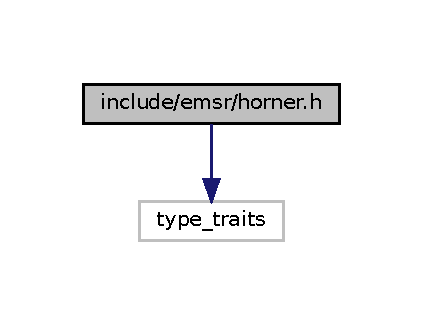
\includegraphics[width=203pt]{horner_8h__incl}
\end{center}
\end{figure}
\doxysubsection*{Namespaces}
\begin{DoxyCompactItemize}
\item 
 \mbox{\hyperlink{namespaceemsr}{emsr}}
\end{DoxyCompactItemize}
\doxysubsection*{Functions}
\begin{DoxyCompactItemize}
\item 
{\footnotesize template$<$typename ArgT , typename Coef0 , typename... Coef$>$ }\\constexpr std\+::conditional\+\_\+t$<$ std\+::is\+\_\+integral$<$ ArgT $>$\+::value, double, ArgT $>$ \mbox{\hyperlink{namespaceemsr_ad76e856347b8d4dc1991d8aad92199f0}{emsr\+::horner}} (ArgT x, Coef0 c0, Coef... c)
\item 
{\footnotesize template$<$typename ArgT , typename Coef0 $>$ }\\constexpr std\+::conditional\+\_\+t$<$ std\+::is\+\_\+integral$<$ ArgT $>$\+::value, double, ArgT $>$ \mbox{\hyperlink{namespaceemsr_a155d146e57554633b51b21e4681ce000}{emsr\+::horner}} (ArgT, Coef0 c0)
\item 
{\footnotesize template$<$typename ArgT , typename Coef1 , typename Coef0 $>$ }\\constexpr std\+::conditional\+\_\+t$<$ std\+::is\+\_\+integral$<$ ArgT $>$\+::value, double, ArgT $>$ \mbox{\hyperlink{namespaceemsr_a381a03247643fc05de000c9d2ccbbe12}{emsr\+::horner\+\_\+big\+\_\+end}} (ArgT x, Coef1 c1, Coef0 c0)
\item 
{\footnotesize template$<$typename ArgT , typename CoefN , typename Coef\+Nm1 , typename... Coef$>$ }\\constexpr std\+::conditional\+\_\+t$<$ std\+::is\+\_\+integral$<$ ArgT $>$\+::value, double, ArgT $>$ \mbox{\hyperlink{namespaceemsr_acc246a38d5dc59a528e6fc7ec3d38b5a}{emsr\+::horner\+\_\+big\+\_\+end}} (ArgT x, CoefN cn, Coef\+Nm1 cnm1, Coef... c)
\item 
{\footnotesize template$<$typename ArgT , typename Coef0 $>$ }\\constexpr std\+::conditional\+\_\+t$<$ std\+::is\+\_\+integral$<$ ArgT $>$\+::value, double, ArgT $>$ \mbox{\hyperlink{namespaceemsr_a55de120e4dc9c5c34075279bdf43d17c}{emsr\+::horner\+\_\+big\+\_\+end}} (ArgT, Coef0 c0)
\end{DoxyCompactItemize}

\hypertarget{polynomial_8h}{}\doxysection{include/emsr/polynomial.h File Reference}
\label{polynomial_8h}\index{include/emsr/polynomial.h@{include/emsr/polynomial.h}}
{\ttfamily \#include $<$initializer\+\_\+list$>$}\newline
{\ttfamily \#include $<$vector$>$}\newline
{\ttfamily \#include $<$iosfwd$>$}\newline
{\ttfamily \#include $<$limits$>$}\newline
{\ttfamily \#include $<$array$>$}\newline
{\ttfamily \#include $<$utility$>$}\newline
{\ttfamily \#include $<$type\+\_\+traits$>$}\newline
{\ttfamily \#include $<$complex$>$}\newline
{\ttfamily \#include $<$emsr/notsospecfun.\+h$>$}\newline
{\ttfamily \#include $<$emsr/polynomial.\+tcc$>$}\newline
Include dependency graph for polynomial.\+h\+:
\nopagebreak
\begin{figure}[H]
\begin{center}
\leavevmode
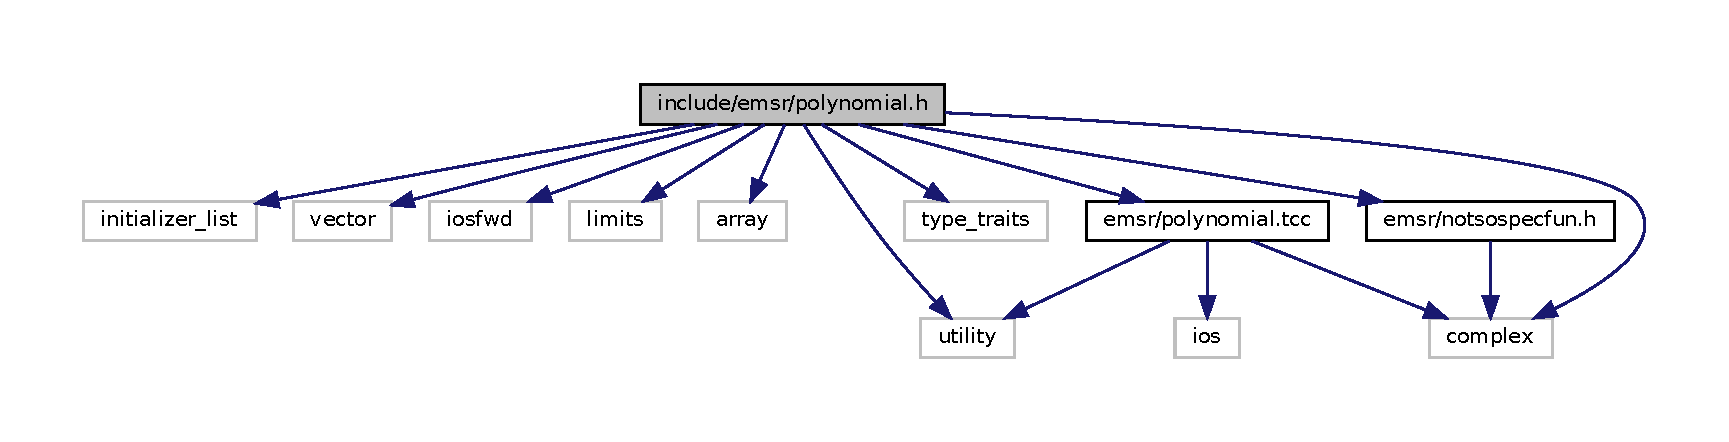
\includegraphics[width=350pt]{polynomial_8h__incl}
\end{center}
\end{figure}
This graph shows which files directly or indirectly include this file\+:
\nopagebreak
\begin{figure}[H]
\begin{center}
\leavevmode
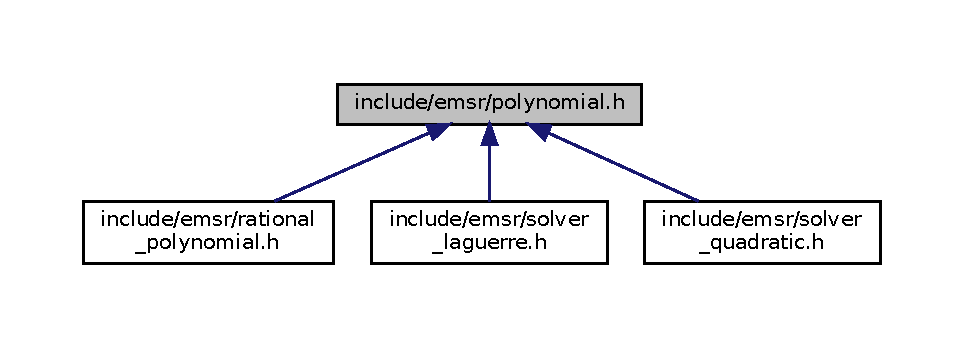
\includegraphics[width=350pt]{polynomial_8h__dep__incl}
\end{center}
\end{figure}
\doxysubsection*{Classes}
\begin{DoxyCompactItemize}
\item 
struct \mbox{\hyperlink{structemsr_1_1has__imag__t}{emsr\+::has\+\_\+imag\+\_\+t$<$ typename, typename $>$}}
\item 
struct \mbox{\hyperlink{structemsr_1_1has__imag__t_3_01Tp_00_01std_1_1void__t_3_01decltype_07std_1_1declval_3_01Tp_01_6_c8fe2aab4cea8d1a1147d770a127d10f}{emsr\+::has\+\_\+imag\+\_\+t$<$ Tp, std\+::void\+\_\+t$<$ decltype(std\+::declval$<$ Tp \& $>$().\+imag())$>$ $>$}}
\item 
struct \mbox{\hyperlink{structemsr_1_1has__value__type__t}{emsr\+::has\+\_\+value\+\_\+type\+\_\+t$<$ typename, typename $>$}}
\item 
struct \mbox{\hyperlink{structemsr_1_1has__value__type__t_3_01Tp_00_01std_1_1void__t_3_01typename_01Tp_1_1value__type_01_4_01_4}{emsr\+::has\+\_\+value\+\_\+type\+\_\+t$<$ Tp, std\+::void\+\_\+t$<$ typename Tp\+::value\+\_\+type $>$ $>$}}
\item 
class \mbox{\hyperlink{classemsr_1_1Polynomial}{emsr\+::\+Polynomial$<$ Tp $>$}}
\begin{DoxyCompactList}\small\item\em A dense polynomial class with a contiguous array of coefficients. The coefficients are lowest-\/order first\+: \end{DoxyCompactList}\item 
struct \mbox{\hyperlink{structemsr_1_1real__type}{emsr\+::real\+\_\+type$<$ Tp $>$}}
\item 
struct \mbox{\hyperlink{structemsr_1_1real__type_3_01Polynomial_3_01Tp_01_4_01_4}{emsr\+::real\+\_\+type$<$ Polynomial$<$ Tp $>$ $>$}}
\item 
struct \mbox{\hyperlink{structemsr_1_1real__type_3_01std_1_1complex_3_01Tp_01_4_01_4}{emsr\+::real\+\_\+type$<$ std\+::complex$<$ Tp $>$ $>$}}
\end{DoxyCompactItemize}
\doxysubsection*{Namespaces}
\begin{DoxyCompactItemize}
\item 
 \mbox{\hyperlink{namespaceemsr}{emsr}}
\end{DoxyCompactItemize}
\doxysubsection*{Typedefs}
\begin{DoxyCompactItemize}
\item 
{\footnotesize template$<$typename Tp $>$ }\\using \mbox{\hyperlink{namespaceemsr_a02ec0ebded7be3a1b57643770c87e413}{emsr\+::real\+\_\+type\+\_\+t}} = typename real\+\_\+type$<$ Tp $>$\+::type
\end{DoxyCompactItemize}
\doxysubsection*{Functions}
\begin{DoxyCompactItemize}
\item 
{\footnotesize template$<$typename Tp $>$ }\\void \mbox{\hyperlink{namespaceemsr_a5d92c91e21caca3557589683df6650c4}{emsr\+::divmod}} (const Polynomial$<$ Tp $>$ \&num, const Polynomial$<$ Tp $>$ \&den, Polynomial$<$ Tp $>$ \&quo, Polynomial$<$ Tp $>$ \&rem)
\item 
{\footnotesize template$<$typename Tp $>$ }\\real\+\_\+type\+\_\+t$<$ Polynomial$<$ Tp $>$ $>$ \mbox{\hyperlink{namespaceemsr_af9fe740b04b1f58f0cafe9042b5a380b}{emsr\+::get\+\_\+scale}} (const Polynomial$<$ Tp $>$ \&poly)
\item 
{\footnotesize template$<$typename Tp $>$ }\\decltype(std\+::abs(Tp())) \mbox{\hyperlink{namespaceemsr_af8bdedf1c9d27acc3695f86d226ca149}{emsr\+::get\+\_\+scale}} (const Tp \&x)
\item 
{\footnotesize template$<$typename Tp $>$ }\\bool \mbox{\hyperlink{namespaceemsr_a16a330b4ef9bcc0f45e8fd412567322e}{emsr\+::operator!=}} (const Polynomial$<$ Tp $>$ \&pa, const Polynomial$<$ Tp $>$ \&pb)
\item 
{\footnotesize template$<$typename Tp , typename Up $>$ }\\Polynomial$<$ decltype(Tp()/Up())$>$ \mbox{\hyperlink{namespaceemsr_adbd25852afa794395ff3c829b2eb023b}{emsr\+::operator\%}} (const Polynomial$<$ Tp $>$ \&pa, const Polynomial$<$ Up $>$ \&pb)
\item 
{\footnotesize template$<$typename Tp , typename Up $>$ }\\Polynomial$<$ decltype(Tp()/Up())$>$ \mbox{\hyperlink{namespaceemsr_aed9775373361a9859b3504c2d9c6bfbb}{emsr\+::operator\%}} (const Polynomial$<$ Tp $>$ \&poly, const Up \&x)
\item 
{\footnotesize template$<$typename Tp , typename Up $>$ }\\Polynomial$<$ decltype(Tp()/Up())$>$ \mbox{\hyperlink{namespaceemsr_ac1b83fde2c334cc77b0a97884ce2ffcd}{emsr\+::operator\%}} (const Tp \&x, const Polynomial$<$ Up $>$ \&poly)
\item 
{\footnotesize template$<$typename Tp , typename Up $>$ }\\Polynomial$<$ decltype(Tp() $\ast$Up())$>$ \mbox{\hyperlink{namespaceemsr_aa8744ef4ccdde86f46197a7da33e0053}{emsr\+::operator$\ast$}} (const Polynomial$<$ Tp $>$ \&pa, const Polynomial$<$ Up $>$ \&pb)
\item 
{\footnotesize template$<$typename Tp , typename Up $>$ }\\Polynomial$<$ decltype(Tp() $\ast$Up())$>$ \mbox{\hyperlink{namespaceemsr_a2a45baf6731916a2509a6c7cecc7fe79}{emsr\+::operator$\ast$}} (const Polynomial$<$ Tp $>$ \&poly, const Up \&x)
\item 
{\footnotesize template$<$typename Tp , typename Up $>$ }\\Polynomial$<$ decltype(Tp() $\ast$Up())$>$ \mbox{\hyperlink{namespaceemsr_a685115a02fab5426320cb39202dc2103}{emsr\+::operator$\ast$}} (const Tp \&x, const Polynomial$<$ Up $>$ \&poly)
\item 
{\footnotesize template$<$typename Tp , typename Up $>$ }\\Polynomial$<$ decltype(Tp()+Up())$>$ \mbox{\hyperlink{namespaceemsr_ac0950a02906dfd97c4e53b76021cdf79}{emsr\+::operator+}} (const Polynomial$<$ Tp $>$ \&pa, const Polynomial$<$ Up $>$ \&pb)
\item 
{\footnotesize template$<$typename Tp , typename Up $>$ }\\Polynomial$<$ decltype(Tp()+Up())$>$ \mbox{\hyperlink{namespaceemsr_a033506a4ee4ccdeec1d2d106715d063d}{emsr\+::operator+}} (const Polynomial$<$ Tp $>$ \&poly, const Up \&x)
\item 
{\footnotesize template$<$typename Tp , typename Up $>$ }\\Polynomial$<$ decltype(Tp()+Up())$>$ \mbox{\hyperlink{namespaceemsr_a403f7be9f19b8cd47e718d94ec8659c1}{emsr\+::operator+}} (const Tp \&x, const Polynomial$<$ Up $>$ \&poly)
\item 
{\footnotesize template$<$typename Tp , typename Up $>$ }\\Polynomial$<$ decltype(Tp() -\/ Up())$>$ \mbox{\hyperlink{namespaceemsr_a843a89e4dfe80c1548a59e70ac2f191c}{emsr\+::operator-\/}} (const Polynomial$<$ Tp $>$ \&pa, const Polynomial$<$ Up $>$ \&pb)
\item 
{\footnotesize template$<$typename Tp , typename Up $>$ }\\Polynomial$<$ decltype(Tp() -\/ Up())$>$ \mbox{\hyperlink{namespaceemsr_afeaf3b7d364a2f3d94396ea631702313}{emsr\+::operator-\/}} (const Polynomial$<$ Tp $>$ \&poly, const Up \&x)
\item 
{\footnotesize template$<$typename Tp , typename Up $>$ }\\Polynomial$<$ decltype(Tp() -\/ Up())$>$ \mbox{\hyperlink{namespaceemsr_a615a0879331fef9a4b9af6175f8e938f}{emsr\+::operator-\/}} (const Tp \&x, const Polynomial$<$ Up $>$ \&poly)
\item 
{\footnotesize template$<$typename Tp , typename Up $>$ }\\Polynomial$<$ decltype(Tp()/Up())$>$ \mbox{\hyperlink{namespaceemsr_a20aabca53f527d2b4c2682e178ed8cbf}{emsr\+::operator/}} (const Polynomial$<$ Tp $>$ \&pa, const Polynomial$<$ Up $>$ \&pb)
\item 
{\footnotesize template$<$typename Tp , typename Up $>$ }\\Polynomial$<$ decltype(Tp()/Up())$>$ \mbox{\hyperlink{namespaceemsr_ac256fc3b7f1798a6b95a612fd291bb4f}{emsr\+::operator/}} (const Polynomial$<$ Tp $>$ \&poly, const Up \&x)
\item 
{\footnotesize template$<$typename Tp , typename Up $>$ }\\Polynomial$<$ decltype(Tp()/Up())$>$ \mbox{\hyperlink{namespaceemsr_a65421cfb10c2b328c5f6fe32394e105a}{emsr\+::operator/}} (const Tp \&x, const Polynomial$<$ Up $>$ \&poly)
\item 
{\footnotesize template$<$typename CharT , typename Traits , typename Tp $>$ }\\std\+::basic\+\_\+ostream$<$ CharT, Traits $>$ \& \mbox{\hyperlink{namespaceemsr_a138fa9753d495e1819e54d43d580720b}{emsr\+::operator$<$$<$}} (std\+::basic\+\_\+ostream$<$ CharT, Traits $>$ \&os, const Polynomial$<$ Tp $>$ \&poly)
\item 
{\footnotesize template$<$typename Tp $>$ }\\bool \mbox{\hyperlink{namespaceemsr_ab9f94cfb4f6d90681c4f279752b486a7}{emsr\+::operator==}} (const Polynomial$<$ Tp $>$ \&pa, const Polynomial$<$ Tp $>$ \&pb)
\item 
{\footnotesize template$<$typename CharT , typename Traits , typename Tp $>$ }\\std\+::basic\+\_\+istream$<$ CharT, Traits $>$ \& \mbox{\hyperlink{namespaceemsr_a93634c3102d6a9a883994cbd19c9cff1}{emsr\+::operator$>$$>$}} (std\+::basic\+\_\+istream$<$ CharT, Traits $>$ \&is, Polynomial$<$ Tp $>$ \&poly)
\item 
{\footnotesize template$<$typename Tp $>$ }\\void \mbox{\hyperlink{namespaceemsr_a8b4e7f7636909dc8a88bc53d81f43eaf}{emsr\+::swap}} (Polynomial$<$ Tp $>$ \&pa, Polynomial$<$ Tp $>$ \&pb) noexcept(noexcept(pa.\+swap(pb)))
\end{DoxyCompactItemize}
\doxysubsection*{Variables}
\begin{DoxyCompactItemize}
\item 
{\footnotesize template$<$typename Tp $>$ }\\constexpr auto \mbox{\hyperlink{namespaceemsr_a5bf2c62dcc64e44b8b65766f71d8aa64}{emsr\+::has\+\_\+imag\+\_\+v}} = has\+\_\+imag\+\_\+t$<$Tp$>$\+::value
\item 
{\footnotesize template$<$typename Tp $>$ }\\constexpr auto \mbox{\hyperlink{namespaceemsr_a59e13ee841ec1f2dbfb09ed021036d3a}{emsr\+::has\+\_\+value\+\_\+type\+\_\+v}} = has\+\_\+value\+\_\+type\+\_\+t$<$Tp$>$\+::value
\end{DoxyCompactItemize}


\doxysubsection{Detailed Description}
Class declaration for a dense univariate polynomial.

This file contains the declaration of a dense-\/polynomial class. 
\hypertarget{polynomial_8tcc}{}\doxysection{include/emsr/polynomial.tcc File Reference}
\label{polynomial_8tcc}\index{include/emsr/polynomial.tcc@{include/emsr/polynomial.tcc}}
{\ttfamily \#include $<$ios$>$}\newline
{\ttfamily \#include $<$complex$>$}\newline
{\ttfamily \#include $<$utility$>$}\newline
Include dependency graph for polynomial.\+tcc\+:\nopagebreak
\begin{figure}[H]
\begin{center}
\leavevmode
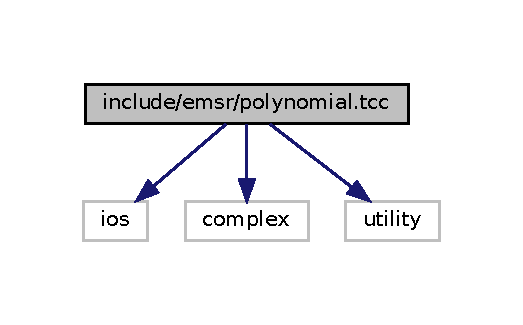
\includegraphics[width=251pt]{polynomial_8tcc__incl}
\end{center}
\end{figure}
This graph shows which files directly or indirectly include this file\+:\nopagebreak
\begin{figure}[H]
\begin{center}
\leavevmode
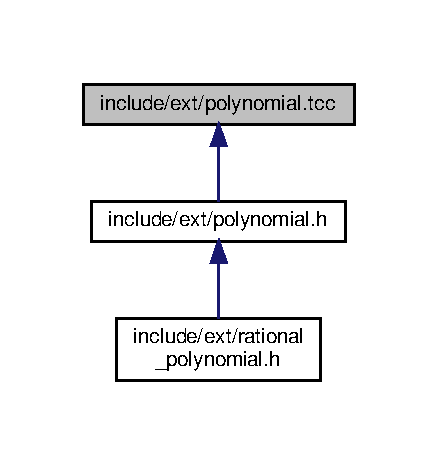
\includegraphics[width=350pt]{polynomial_8tcc__dep__incl}
\end{center}
\end{figure}
\doxysubsection*{Namespaces}
\begin{DoxyCompactItemize}
\item 
 \mbox{\hyperlink{namespaceemsr}{emsr}}
\end{DoxyCompactItemize}
\doxysubsection*{Macros}
\begin{DoxyCompactItemize}
\item 
\#define \mbox{\hyperlink{polynomial_8tcc_a21cfc48b0e3feb3f580228c01773d9c8}{POLYNOMIAL\+\_\+\+TCC}}~1
\begin{DoxyCompactList}\small\item\em A guard for the polynomial class implementation header. \end{DoxyCompactList}\end{DoxyCompactItemize}
\doxysubsection*{Functions}
\begin{DoxyCompactItemize}
\item 
{\footnotesize template$<$typename Tp $>$ }\\void \mbox{\hyperlink{namespaceemsr_a5d92c91e21caca3557589683df6650c4}{emsr\+::divmod}} (const Polynomial$<$ Tp $>$ \&num, const Polynomial$<$ Tp $>$ \&den, Polynomial$<$ Tp $>$ \&quo, Polynomial$<$ Tp $>$ \&rem)
\item 
{\footnotesize template$<$typename CharT , typename Traits , typename Tp $>$ }\\std\+::basic\+\_\+ostream$<$ CharT, Traits $>$ \& \mbox{\hyperlink{namespaceemsr_a138fa9753d495e1819e54d43d580720b}{emsr\+::operator$<$$<$}} (std\+::basic\+\_\+ostream$<$ CharT, Traits $>$ \&os, const Polynomial$<$ Tp $>$ \&poly)
\item 
{\footnotesize template$<$typename CharT , typename Traits , typename Tp $>$ }\\std\+::basic\+\_\+istream$<$ CharT, Traits $>$ \& \mbox{\hyperlink{namespaceemsr_a93634c3102d6a9a883994cbd19c9cff1}{emsr\+::operator$>$$>$}} (std\+::basic\+\_\+istream$<$ CharT, Traits $>$ \&is, Polynomial$<$ Tp $>$ \&poly)
\end{DoxyCompactItemize}


\doxysubsection{Detailed Description}
Out-\/of-\/line definitions of members for a dense univariate polynomial.

This file contains the out-\/of-\/line implementations of the polynomial class.

\begin{DoxySeeAlso}{See also}
\mbox{\hyperlink{polynomial_8h}{polynomial.\+h}} 
\end{DoxySeeAlso}


\doxysubsection{Macro Definition Documentation}
\mbox{\Hypertarget{polynomial_8tcc_a21cfc48b0e3feb3f580228c01773d9c8}\label{polynomial_8tcc_a21cfc48b0e3feb3f580228c01773d9c8}} 
\index{polynomial.tcc@{polynomial.tcc}!POLYNOMIAL\_TCC@{POLYNOMIAL\_TCC}}
\index{POLYNOMIAL\_TCC@{POLYNOMIAL\_TCC}!polynomial.tcc@{polynomial.tcc}}
\doxysubsubsection{\texorpdfstring{POLYNOMIAL\_TCC}{POLYNOMIAL\_TCC}}
{\footnotesize\ttfamily \#define POLYNOMIAL\+\_\+\+TCC~1}



A guard for the polynomial class implementation header. 



Definition at line 39 of file polynomial.\+tcc.


\hypertarget{rational__polynomial_8h}{}\doxysection{include/emsr/rational\+\_\+polynomial.h File Reference}
\label{rational__polynomial_8h}\index{include/emsr/rational\_polynomial.h@{include/emsr/rational\_polynomial.h}}
{\ttfamily \#include $<$iostream$>$}\newline
{\ttfamily \#include $<$emsr/polynomial.\+h$>$}\newline
Include dependency graph for rational\+\_\+polynomial.\+h\+:\nopagebreak
\begin{figure}[H]
\begin{center}
\leavevmode
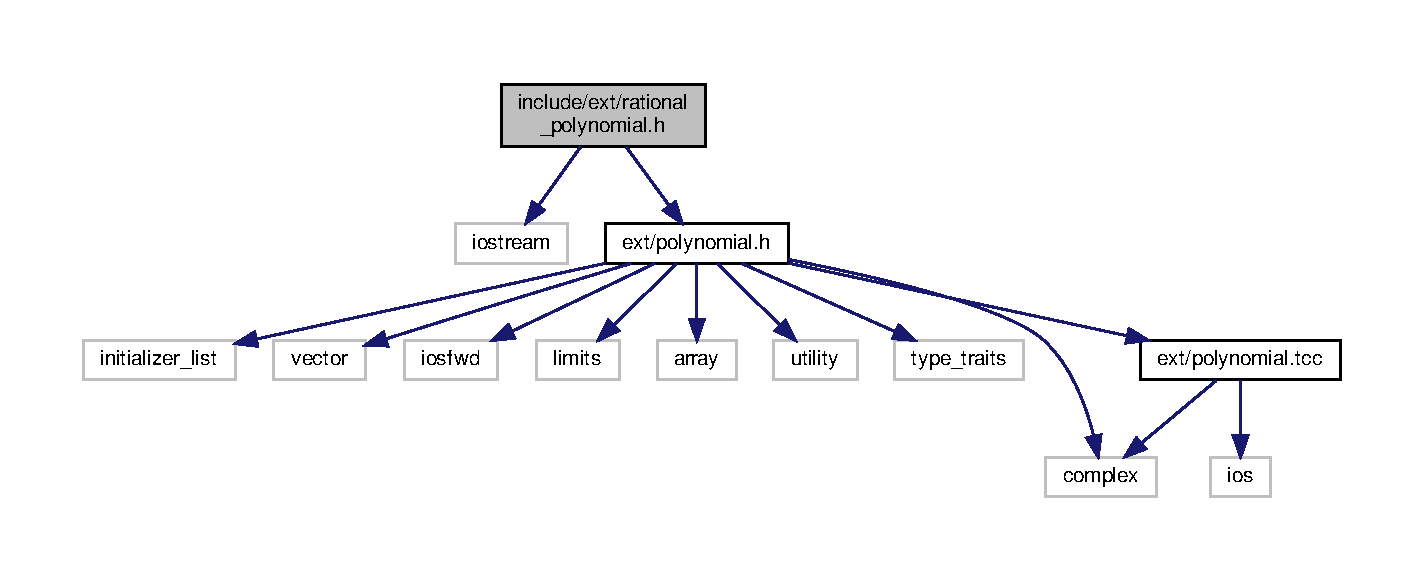
\includegraphics[width=350pt]{rational__polynomial_8h__incl}
\end{center}
\end{figure}
\doxysubsection*{Classes}
\begin{DoxyCompactItemize}
\item 
class \mbox{\hyperlink{classemsr_1_1RationalPolynomial}{emsr\+::\+Rational\+Polynomial$<$ Tp $>$}}
\end{DoxyCompactItemize}
\doxysubsection*{Namespaces}
\begin{DoxyCompactItemize}
\item 
 \mbox{\hyperlink{namespaceemsr}{emsr}}
\end{DoxyCompactItemize}
\doxysubsection*{Functions}
\begin{DoxyCompactItemize}
\item 
{\footnotesize template$<$typename CharT , typename Traits , typename Tp $>$ }\\std\+::basic\+\_\+ostream$<$ CharT, Traits $>$ \& \mbox{\hyperlink{namespaceemsr_aefffa447e50d21ac578b5c3aafc992e2}{emsr\+::operator$<$$<$}} (std\+::basic\+\_\+ostream$<$ CharT, Traits $>$ \&os, const Rational\+Polynomial$<$ Tp $>$ \&poly)
\item 
{\footnotesize template$<$typename CharT , typename Traits , typename Tp $>$ }\\std\+::basic\+\_\+istream$<$ CharT, Traits $>$ \& \mbox{\hyperlink{namespaceemsr_a0fa608fda96ca8649cbdb86338e69846}{emsr\+::operator$>$$>$}} (std\+::basic\+\_\+istream$<$ CharT, Traits $>$ \&is, Rational\+Polynomial$<$ Tp $>$ \&poly)
\end{DoxyCompactItemize}


\doxysubsection{Detailed Description}
This file contains the declaration of a ratio of two polynomials. \begin{DoxySeeAlso}{See also}
\mbox{\hyperlink{polynomial_8h}{polynomial.\+h}} 
\end{DoxySeeAlso}

\hypertarget{solution_8h}{}\doxysection{include/emsr/solution.h File Reference}
\label{solution_8h}\index{include/emsr/solution.h@{include/emsr/solution.h}}
{\ttfamily \#include $<$complex$>$}\newline
{\ttfamily \#include $<$variant$>$}\newline
{\ttfamily \#include $<$iosfwd$>$}\newline
Include dependency graph for solution.\+h\+:\nopagebreak
\begin{figure}[H]
\begin{center}
\leavevmode
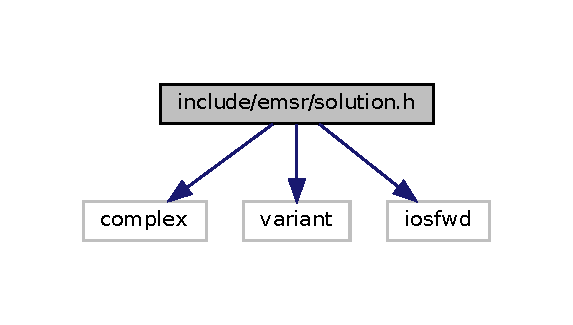
\includegraphics[width=275pt]{solution_8h__incl}
\end{center}
\end{figure}
This graph shows which files directly or indirectly include this file\+:\nopagebreak
\begin{figure}[H]
\begin{center}
\leavevmode
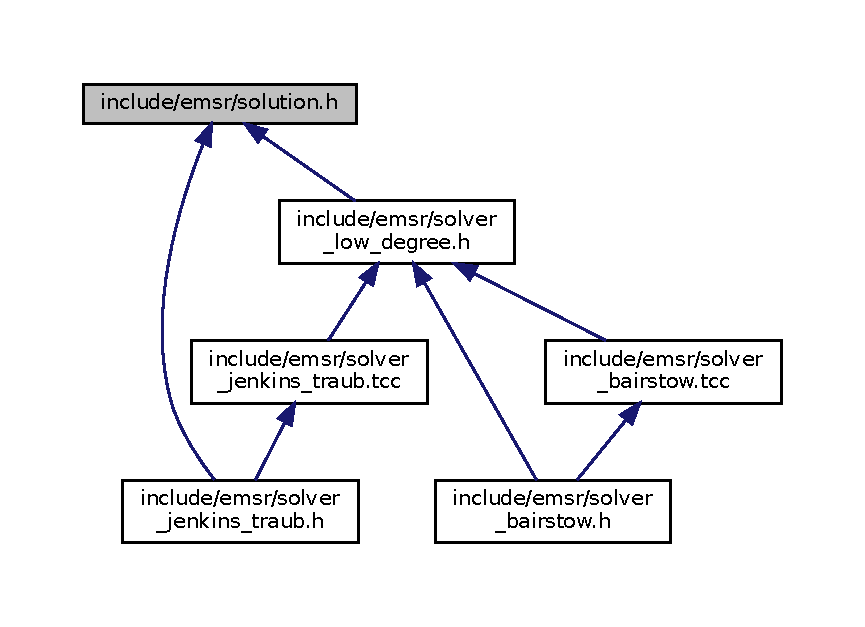
\includegraphics[width=350pt]{solution_8h__dep__incl}
\end{center}
\end{figure}
\doxysubsection*{Classes}
\begin{DoxyCompactItemize}
\item 
struct \mbox{\hyperlink{structemsr_1_1Solution}{emsr\+::\+Solution$<$ Real $>$}}
\end{DoxyCompactItemize}
\doxysubsection*{Namespaces}
\begin{DoxyCompactItemize}
\item 
 \mbox{\hyperlink{namespaceemsr}{emsr}}
\end{DoxyCompactItemize}
\doxysubsection*{Functions}
\begin{DoxyCompactItemize}
\item 
{\footnotesize template$<$typename Real $>$ }\\constexpr Real \mbox{\hyperlink{namespaceemsr_a782d36096e8467b4a45a9dc2f89355b2}{emsr\+::abs}} (const Solution$<$ Real $>$ \&x)
\item 
{\footnotesize template$<$typename Real $>$ }\\constexpr Real \mbox{\hyperlink{namespaceemsr_a79ddc0cda81a11ab065e5caae9e0907a}{emsr\+::imag}} (const Solution$<$ Real $>$ \&x)
\item 
{\footnotesize template$<$typename Real $>$ }\\constexpr bool \mbox{\hyperlink{namespaceemsr_ad500d5a09de89975430355fd46c9be25}{emsr\+::is\+\_\+valid}} (const Solution$<$ Real $>$ \&x)
\item 
{\footnotesize template$<$typename Real $>$ }\\constexpr bool \mbox{\hyperlink{namespaceemsr_ad52e42498f67025febd9075ad75b0645}{emsr\+::operator!=}} (const Solution$<$ Real $>$ \&x, const Solution$<$ Real $>$ \&y)
\item 
{\footnotesize template$<$typename Real $>$ }\\constexpr bool \mbox{\hyperlink{namespaceemsr_a65037c6f423a051e29798d1039949525}{emsr\+::operator!=}} (const Solution$<$ Real $>$ \&x, const std\+::complex$<$ Real $>$ \&y)
\item 
{\footnotesize template$<$typename Real $>$ }\\bool \mbox{\hyperlink{namespaceemsr_ab7fc1800f8665163ddee970a134d64bb}{emsr\+::operator!=}} (const Solution$<$ Real $>$ \&x, Real y)
\item 
{\footnotesize template$<$typename Real $>$ }\\constexpr bool \mbox{\hyperlink{namespaceemsr_a7dbf4dea4cebcd849d6c9d6811289073}{emsr\+::operator!=}} (const std\+::complex$<$ Real $>$ \&x, const Solution$<$ Real $>$ \&y)
\item 
{\footnotesize template$<$typename Real $>$ }\\constexpr bool \mbox{\hyperlink{namespaceemsr_a1ca6592331d19bfa53c432a5ea9f442e}{emsr\+::operator!=}} (Real x, const Solution$<$ Real $>$ \&y)
\item 
{\footnotesize template$<$typename Real $>$ }\\constexpr Solution$<$ Real $>$ \mbox{\hyperlink{namespaceemsr_aabff597754fb0244c190e91bb6f26fd4}{emsr\+::operator$\ast$}} (const Solution$<$ Real $>$ \&x, const Solution$<$ Real $>$ \&y)
\item 
{\footnotesize template$<$typename Real $>$ }\\constexpr Solution$<$ Real $>$ \mbox{\hyperlink{namespaceemsr_a4a8d3aa3a28f77da8940fac42aff11d4}{emsr\+::operator$\ast$}} (const Solution$<$ Real $>$ \&x, const std\+::complex$<$ Real $>$ \&y)
\item 
{\footnotesize template$<$typename Real $>$ }\\constexpr Solution$<$ Real $>$ \mbox{\hyperlink{namespaceemsr_a8a39231a5577174cc0db572a71551596}{emsr\+::operator$\ast$}} (const Solution$<$ Real $>$ \&x, Real y)
\item 
{\footnotesize template$<$typename Real $>$ }\\constexpr Solution$<$ Real $>$ \mbox{\hyperlink{namespaceemsr_af5909d8b89e4fe1928b93a5be6f1058c}{emsr\+::operator$\ast$}} (const std\+::complex$<$ Real $>$ \&x, const Solution$<$ Real $>$ \&y)
\item 
{\footnotesize template$<$typename Real $>$ }\\constexpr Solution$<$ Real $>$ \mbox{\hyperlink{namespaceemsr_a532d30a3725f3b9f83ff768947a20d2b}{emsr\+::operator$\ast$}} (Real x, const Solution$<$ Real $>$ \&y)
\item 
{\footnotesize template$<$typename Real $>$ }\\constexpr Solution$<$ Real $>$ \mbox{\hyperlink{namespaceemsr_a0cc7606f0dde0b46384b29879ee9537e}{emsr\+::operator+}} (const Solution$<$ Real $>$ \&x)
\item 
{\footnotesize template$<$typename Real $>$ }\\constexpr Solution$<$ Real $>$ \mbox{\hyperlink{namespaceemsr_a9b70158ac63e2c4ff91a23f962b10597}{emsr\+::operator+}} (const Solution$<$ Real $>$ \&x, const Solution$<$ Real $>$ \&y)
\item 
{\footnotesize template$<$typename Real $>$ }\\constexpr Solution$<$ Real $>$ \mbox{\hyperlink{namespaceemsr_a8f1d6fe31e0864c5336cece2a58cdb44}{emsr\+::operator+}} (const Solution$<$ Real $>$ \&x, const std\+::complex$<$ Real $>$ \&y)
\item 
{\footnotesize template$<$typename Real $>$ }\\constexpr Solution$<$ Real $>$ \mbox{\hyperlink{namespaceemsr_afae0ae20027dc5a2044b9d6dd9534227}{emsr\+::operator+}} (const Solution$<$ Real $>$ \&x, Real y)
\item 
{\footnotesize template$<$typename Real $>$ }\\constexpr Solution$<$ Real $>$ \mbox{\hyperlink{namespaceemsr_adf385890f1a6fa020b1773ba53d00310}{emsr\+::operator+}} (const std\+::complex$<$ Real $>$ \&x, const Solution$<$ Real $>$ \&y)
\item 
{\footnotesize template$<$typename Real $>$ }\\constexpr Solution$<$ Real $>$ \mbox{\hyperlink{namespaceemsr_ab946e0e685c1304a6e9e249e837061a4}{emsr\+::operator+}} (Real x, const Solution$<$ Real $>$ \&y)
\item 
{\footnotesize template$<$typename Real $>$ }\\constexpr Solution$<$ Real $>$ \mbox{\hyperlink{namespaceemsr_a434a04338777c51fec03a803df64f1ea}{emsr\+::operator-\/}} (const Solution$<$ Real $>$ \&x)
\item 
{\footnotesize template$<$typename Real $>$ }\\constexpr Solution$<$ Real $>$ \mbox{\hyperlink{namespaceemsr_ab571b1b9099153a1aba906a25e238dfa}{emsr\+::operator-\/}} (const Solution$<$ Real $>$ \&x, const Solution$<$ Real $>$ \&y)
\item 
{\footnotesize template$<$typename Real $>$ }\\constexpr Solution$<$ Real $>$ \mbox{\hyperlink{namespaceemsr_abb04a325d56ca7ee1ee8b4ced1a15800}{emsr\+::operator-\/}} (const Solution$<$ Real $>$ \&x, const std\+::complex$<$ Real $>$ \&y)
\item 
{\footnotesize template$<$typename Real $>$ }\\constexpr Solution$<$ Real $>$ \mbox{\hyperlink{namespaceemsr_a1d0395812f51330c8690936c11f9a526}{emsr\+::operator-\/}} (const Solution$<$ Real $>$ \&x, Real y)
\item 
{\footnotesize template$<$typename Real $>$ }\\constexpr Solution$<$ Real $>$ \mbox{\hyperlink{namespaceemsr_af0e20c39abb723a3c8a6d6c81ad5b681}{emsr\+::operator-\/}} (const std\+::complex$<$ Real $>$ \&x, const Solution$<$ Real $>$ \&y)
\item 
{\footnotesize template$<$typename Real $>$ }\\constexpr Solution$<$ Real $>$ \mbox{\hyperlink{namespaceemsr_a016df2328f39b176fcd5c22f612497a0}{emsr\+::operator-\/}} (Real x, const Solution$<$ Real $>$ \&y)
\item 
{\footnotesize template$<$typename Real $>$ }\\constexpr Solution$<$ Real $>$ \mbox{\hyperlink{namespaceemsr_aae74c8d59cd3b187fc89692d21fb6aec}{emsr\+::operator/}} (const Solution$<$ Real $>$ \&x, const Solution$<$ Real $>$ \&y)
\item 
{\footnotesize template$<$typename Real $>$ }\\constexpr Solution$<$ Real $>$ \mbox{\hyperlink{namespaceemsr_a5b53a2571ed1de735c01abe73604730f}{emsr\+::operator/}} (const Solution$<$ Real $>$ \&x, const std\+::complex$<$ Real $>$ \&y)
\item 
{\footnotesize template$<$typename Real $>$ }\\constexpr Solution$<$ Real $>$ \mbox{\hyperlink{namespaceemsr_a1ddf836180b255c273560c94ba78aa3e}{emsr\+::operator/}} (const Solution$<$ Real $>$ \&x, Real y)
\item 
{\footnotesize template$<$typename Real $>$ }\\constexpr Solution$<$ Real $>$ \mbox{\hyperlink{namespaceemsr_a0151e61717cae6662ea239b3a2433d89}{emsr\+::operator/}} (const std\+::complex$<$ Real $>$ \&x, const Solution$<$ Real $>$ \&y)
\item 
{\footnotesize template$<$typename Real $>$ }\\constexpr Solution$<$ Real $>$ \mbox{\hyperlink{namespaceemsr_a0e523c350964ac38101a06d45484f65a}{emsr\+::operator/}} (Real x, const Solution$<$ Real $>$ \&y)
\item 
{\footnotesize template$<$typename Real $>$ }\\constexpr bool \mbox{\hyperlink{namespaceemsr_a348aa4c91f5141addb4006973a934bd7}{emsr\+::operator$<$}} (const Solution$<$ Real $>$ \&x, const Solution$<$ Real $>$ \&y)
\item 
{\footnotesize template$<$typename Real $>$ }\\constexpr bool \mbox{\hyperlink{namespaceemsr_a651793a53daa6800efcd4d711b0dc8bf}{emsr\+::operator$<$}} (const Solution$<$ Real $>$ \&x, const std\+::complex$<$ Real $>$ \&y)
\item 
{\footnotesize template$<$typename Real $>$ }\\constexpr bool \mbox{\hyperlink{namespaceemsr_a1414352fb5db1523b704004efe6491e8}{emsr\+::operator$<$}} (const Solution$<$ Real $>$ \&x, Real y)
\item 
{\footnotesize template$<$typename Real $>$ }\\constexpr bool \mbox{\hyperlink{namespaceemsr_a59cee564d7a746ef2606609a28f90fa1}{emsr\+::operator$<$}} (const std\+::complex$<$ Real $>$ \&x, const Solution$<$ Real $>$ \&y)
\item 
{\footnotesize template$<$typename Real $>$ }\\constexpr bool \mbox{\hyperlink{namespaceemsr_a33f75a43bf27f6102ddef9ce53dfe4ab}{emsr\+::operator$<$}} (Real x, const Solution$<$ Real $>$ \&y)
\item 
{\footnotesize template$<$typename Char , typename Real $>$ }\\std\+::basic\+\_\+ostream$<$ Char $>$ \& \mbox{\hyperlink{namespaceemsr_a926f40da1c865e89a91b9f151c1e3346}{emsr\+::operator$<$$<$}} (std\+::basic\+\_\+ostream$<$ Char $>$ \&out, const \mbox{\hyperlink{structemsr_1_1Solution}{emsr\+::\+Solution}}$<$ Real $>$ \&sln)
\item 
{\footnotesize template$<$typename Real $>$ }\\constexpr bool \mbox{\hyperlink{namespaceemsr_a347cae7848e69cee8176eac10e5b9318}{emsr\+::operator==}} (const Solution$<$ Real $>$ \&x, const Solution$<$ Real $>$ \&y)
\item 
{\footnotesize template$<$typename Real $>$ }\\constexpr bool \mbox{\hyperlink{namespaceemsr_a8196fd2e8625f2b62cee678b1022a90a}{emsr\+::operator==}} (const Solution$<$ Real $>$ \&x, const std\+::complex$<$ Real $>$ \&y)
\item 
{\footnotesize template$<$typename Real $>$ }\\bool \mbox{\hyperlink{namespaceemsr_a7319379b40a854772a1d399db164c920}{emsr\+::operator==}} (const Solution$<$ Real $>$ \&x, Real y)
\item 
{\footnotesize template$<$typename Real $>$ }\\constexpr bool \mbox{\hyperlink{namespaceemsr_a392d7f9e0468d80cd6b8067a133d139e}{emsr\+::operator==}} (const std\+::complex$<$ Real $>$ \&x, const Solution$<$ Real $>$ \&y)
\item 
{\footnotesize template$<$typename Real $>$ }\\constexpr bool \mbox{\hyperlink{namespaceemsr_a6e5d604182a149e63b319c13f72ccad3}{emsr\+::operator==}} (Real x, const Solution$<$ Real $>$ \&y)
\item 
{\footnotesize template$<$typename Real $>$ }\\constexpr Real \mbox{\hyperlink{namespaceemsr_a3b69f1c91fb3480e098db4e4bfe949f2}{emsr\+::real}} (const Solution$<$ Real $>$ \&x)
\item 
{\footnotesize template$<$typename Real $>$ }\\constexpr Solution$<$ Real $>$ \mbox{\hyperlink{namespaceemsr_a31fe15f97bf442f3b709d901904a5c72}{emsr\+::to\+\_\+complex}} (const Solution$<$ Real $>$ \&x)
\end{DoxyCompactItemize}


\doxysubsection{Detailed Description}
This file contains a type representing a solution of a polynomial. The soution could be null, i.\+e. on-\/existent. If it exists it could be real of complex. 
\hypertarget{solver__low__degree_8h}{}\doxysection{include/emsr/solver\+\_\+low\+\_\+degree.h File Reference}
\label{solver__low__degree_8h}\index{include/emsr/solver\_low\_degree.h@{include/emsr/solver\_low\_degree.h}}
{\ttfamily \#include $<$array$>$}\newline
{\ttfamily \#include $<$emsr/solution.\+h$>$}\newline
{\ttfamily \#include $<$emsr/solver\+\_\+low\+\_\+degree.\+tcc$>$}\newline
Include dependency graph for solver\+\_\+low\+\_\+degree.\+h\+:
\nopagebreak
\begin{figure}[H]
\begin{center}
\leavevmode
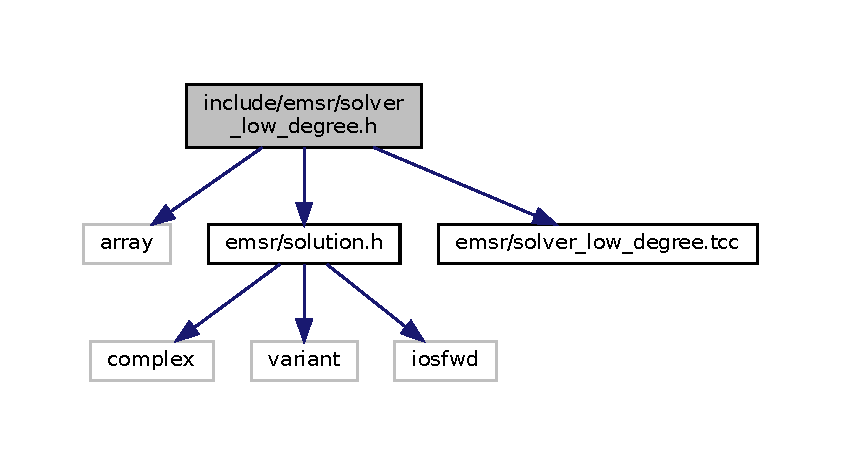
\includegraphics[width=350pt]{solver__low__degree_8h__incl}
\end{center}
\end{figure}
This graph shows which files directly or indirectly include this file\+:\nopagebreak
\begin{figure}[H]
\begin{center}
\leavevmode
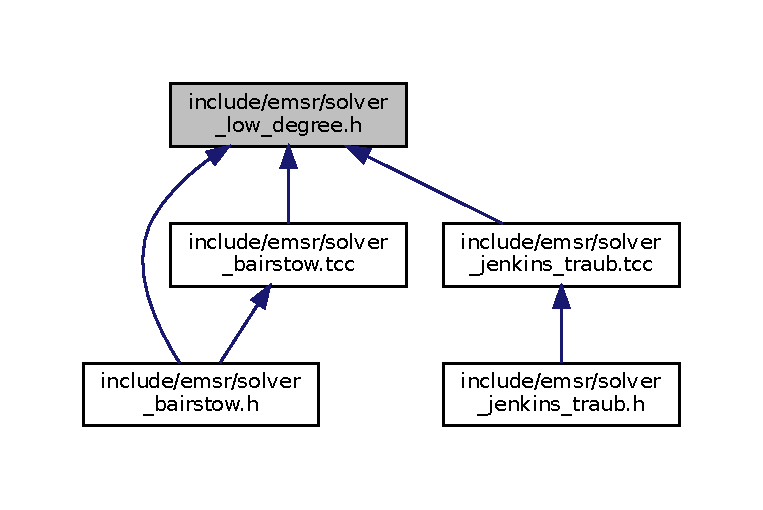
\includegraphics[width=350pt]{solver__low__degree_8h__dep__incl}
\end{center}
\end{figure}
\doxysubsection*{Namespaces}
\begin{DoxyCompactItemize}
\item 
 \mbox{\hyperlink{namespaceemsr}{emsr}}
\end{DoxyCompactItemize}
\doxysubsection*{Functions}
\begin{DoxyCompactItemize}
\item 
{\footnotesize template$<$typename Real , typename Iter $>$ }\\std\+::array$<$ Solution$<$ Real $>$, 3 $>$ \mbox{\hyperlink{namespaceemsr_affe4f64b8e546b29054514e013560ea0}{emsr\+::cubic}} (const Iter \&CC)
\begin{DoxyCompactList}\small\item\em Finds the roots of a cubic equation of the form\+: \end{DoxyCompactList}\item 
{\footnotesize template$<$typename Real $>$ }\\std\+::array$<$ Solution$<$ Real $>$, 3 $>$ \mbox{\hyperlink{namespaceemsr_ad78d9f421df742cad9c10eb3c753f7b8}{emsr\+::cubic}} (Real c0, Real c1, Real c2, Real c3)
\item 
{\footnotesize template$<$typename Real , typename Iter $>$ }\\std\+::array$<$ Solution$<$ Real $>$, 2 $>$ \mbox{\hyperlink{namespaceemsr_a00b524d40ae2c1c9a280df4408c8fed2}{emsr\+::quadratic}} (const Iter \&coef)
\item 
{\footnotesize template$<$typename Real $>$ }\\std\+::array$<$ Solution$<$ Real $>$, 2 $>$ \mbox{\hyperlink{namespaceemsr_a2da681638d9a291cfbc004aac518e8ee}{emsr\+::quadratic}} (Real c0, Real c1, Real c2)
\item 
{\footnotesize template$<$typename Real , typename Iter $>$ }\\std\+::array$<$ Solution$<$ Real $>$, 4 $>$ \mbox{\hyperlink{namespaceemsr_a822edeea9a631fdca6bd4634d67ee02e}{emsr\+::quartic}} (const Iter \&CC)
\begin{DoxyCompactList}\small\item\em Finds the roots a quartic equation of the form\+: \end{DoxyCompactList}\item 
{\footnotesize template$<$typename Real $>$ }\\std\+::array$<$ Solution$<$ Real $>$, 4 $>$ \mbox{\hyperlink{namespaceemsr_aa267aed0e5f2d4e6b290d99dad0bb87f}{emsr\+::quartic}} (Real c0, Real c1, Real c2, Real c3, Real c4)
\item 
{\footnotesize template$<$std\+::size\+\_\+t Dim, typename Iter , typename Num\+Tp $>$ }\\Num\+Tp \mbox{\hyperlink{namespaceemsr_aa39848f35781685f7348bd000d4c8f04}{emsr\+::refine\+\_\+solution\+\_\+halley}} (Num\+Tp z, const Iter \&CC)
\item 
{\footnotesize template$<$std\+::size\+\_\+t Dim, typename Iter , typename Num\+Tp $>$ }\\Num\+Tp \mbox{\hyperlink{namespaceemsr_a0c391643349e3d33d22c04af7e639e59}{emsr\+::refine\+\_\+solution\+\_\+newton}} (Num\+Tp z, const Iter \&CC)
\end{DoxyCompactItemize}


\doxysubsection{Detailed Description}
This file is a GNU extension to the Standard C++ Library.

This file contains the declarations of free functions for solving quadratic, cubic, and quartic equations with real coefficients.

This file is a GNU extension to the Standard C++ Library.

This file contains the definitions of free functions for solving quadratic, cubic, and quartic equations with real coefficients. 
\hypertarget{solver__low__degree_8tcc}{}\section{include/ext/solver\+\_\+low\+\_\+degree.tcc File Reference}
\label{solver__low__degree_8tcc}\index{include/ext/solver\+\_\+low\+\_\+degree.\+tcc@{include/ext/solver\+\_\+low\+\_\+degree.\+tcc}}
{\ttfamily \#include $<$ext/math\+\_\+constants.\+h$>$}\newline
Include dependency graph for solver\+\_\+low\+\_\+degree.\+tcc\+:
\nopagebreak
\begin{figure}[H]
\begin{center}
\leavevmode
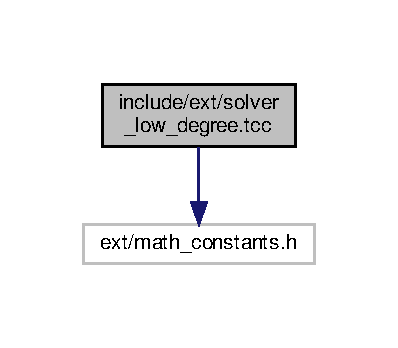
\includegraphics[width=191pt]{solver__low__degree_8tcc__incl}
\end{center}
\end{figure}
This graph shows which files directly or indirectly include this file\+:
\nopagebreak
\begin{figure}[H]
\begin{center}
\leavevmode
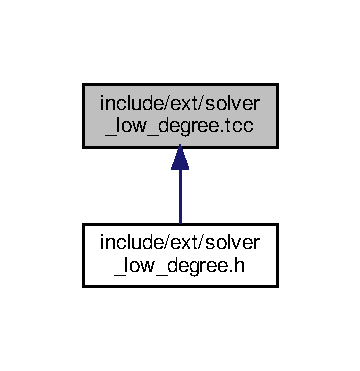
\includegraphics[width=173pt]{solver__low__degree_8tcc__dep__incl}
\end{center}
\end{figure}
\subsection*{Namespaces}
\begin{DoxyCompactItemize}
\item 
 \hyperlink{namespace____gnu__cxx}{\+\_\+\+\_\+gnu\+\_\+cxx}
\end{DoxyCompactItemize}
\subsection*{Macros}
\begin{DoxyCompactItemize}
\item 
\#define \hyperlink{solver__low__degree_8tcc_a10202d26918e17d656cf14da05e26477}{\+\_\+\+E\+X\+T\+\_\+\+S\+O\+L\+V\+E\+R\+\_\+\+L\+O\+W\+\_\+\+D\+E\+G\+R\+E\+E\+\_\+\+T\+CC}~1
\begin{DoxyCompactList}\small\item\em A guard for the low-\/degree polynomial solver functions header. \end{DoxyCompactList}\end{DoxyCompactItemize}
\subsection*{Functions}
\begin{DoxyCompactItemize}
\item 
{\footnotesize template$<$typename \+\_\+\+Real , typename \+\_\+\+Iter $>$ }\\std\+::array$<$ solution\+\_\+t$<$ \+\_\+\+Real $>$, 3 $>$ \hyperlink{namespace____gnu__cxx_a422f638b186be2071012321de5f9bb48}{\+\_\+\+\_\+gnu\+\_\+cxx\+::\+\_\+\+\_\+cubic} (const \+\_\+\+Iter \&\+\_\+\+CC)
\begin{DoxyCompactList}\small\item\em Finds the roots of a cubic equation of the form\+: \[ a_3 x^3 + a_2 x^2 + a_1 x + a_0 = 0 \] for real coefficients $ a_k $. \end{DoxyCompactList}\item 
{\footnotesize template$<$typename \+\_\+\+Real , typename \+\_\+\+Iter $>$ }\\std\+::array$<$ solution\+\_\+t$<$ \+\_\+\+Real $>$, 2 $>$ \hyperlink{namespace____gnu__cxx_aa8c3d98e6508a1e20a17c5980ccbbd99}{\+\_\+\+\_\+gnu\+\_\+cxx\+::\+\_\+\+\_\+quadratic} (const \+\_\+\+Iter \&\+\_\+\+CC)
\begin{DoxyCompactList}\small\item\em Finds the roots of a quadratic equation of the form\+: \[ a_2 x^2 + a_1 x + a_0 = 0 \] for real coefficients $ a_k $. \end{DoxyCompactList}\item 
{\footnotesize template$<$typename \+\_\+\+Real , typename \+\_\+\+Iter $>$ }\\std\+::array$<$ solution\+\_\+t$<$ \+\_\+\+Real $>$, 4 $>$ \hyperlink{namespace____gnu__cxx_ac813fbad739bf1d431845d5175f24701}{\+\_\+\+\_\+gnu\+\_\+cxx\+::\+\_\+\+\_\+quartic} (const \+\_\+\+Iter \&\+\_\+\+CC)
\begin{DoxyCompactList}\small\item\em Finds the roots a quartic equation of the form\+: \[ a_4 x^4 + a_3 x^3 + a_2 x^2 + a_1 x + a_0 = 0 \] for real coefficients $ a_k $. \end{DoxyCompactList}\item 
{\footnotesize template$<$std\+::size\+\_\+t \+\_\+\+Dim, typename \+\_\+\+Iter , typename \+\_\+\+Num\+Tp $>$ }\\\+\_\+\+Num\+Tp \hyperlink{namespace____gnu__cxx_a957b92036746a66f3dff0c46cb18120b}{\+\_\+\+\_\+gnu\+\_\+cxx\+::\+\_\+\+\_\+refine\+\_\+solution\+\_\+halley} (\+\_\+\+Num\+Tp \+\_\+\+\_\+z, const \+\_\+\+Iter \&\+\_\+\+CC)
\item 
{\footnotesize template$<$std\+::size\+\_\+t \+\_\+\+Dim, typename \+\_\+\+Iter , typename \+\_\+\+Num\+Tp $>$ }\\\+\_\+\+Num\+Tp \hyperlink{namespace____gnu__cxx_a2b802e73df33cafb7f95800cbca6ff30}{\+\_\+\+\_\+gnu\+\_\+cxx\+::\+\_\+\+\_\+refine\+\_\+solution\+\_\+newton} (\+\_\+\+Num\+Tp \+\_\+\+\_\+z, const \+\_\+\+Iter \&\+\_\+\+CC)
\item 
{\footnotesize template$<$std\+::size\+\_\+t \+\_\+\+Dim, typename \+\_\+\+Iter , typename \+\_\+\+Real $>$ }\\void \hyperlink{namespace____gnu__cxx_aa8dd4c7542667cc5a8e435ca53d6fad7}{\+\_\+\+\_\+gnu\+\_\+cxx\+::\+\_\+\+\_\+refine\+\_\+solutions} (std\+::array$<$ solution\+\_\+t$<$ \+\_\+\+Real $>$, \+\_\+\+Dim -\/ 1 $>$ \&\+\_\+\+ZZ, const \+\_\+\+Iter \&\+\_\+\+CC)
\end{DoxyCompactItemize}


\subsection{Macro Definition Documentation}
\mbox{\Hypertarget{solver__low__degree_8tcc_a10202d26918e17d656cf14da05e26477}\label{solver__low__degree_8tcc_a10202d26918e17d656cf14da05e26477}} 
\index{solver\+\_\+low\+\_\+degree.\+tcc@{solver\+\_\+low\+\_\+degree.\+tcc}!\+\_\+\+E\+X\+T\+\_\+\+S\+O\+L\+V\+E\+R\+\_\+\+L\+O\+W\+\_\+\+D\+E\+G\+R\+E\+E\+\_\+\+T\+CC@{\+\_\+\+E\+X\+T\+\_\+\+S\+O\+L\+V\+E\+R\+\_\+\+L\+O\+W\+\_\+\+D\+E\+G\+R\+E\+E\+\_\+\+T\+CC}}
\index{\+\_\+\+E\+X\+T\+\_\+\+S\+O\+L\+V\+E\+R\+\_\+\+L\+O\+W\+\_\+\+D\+E\+G\+R\+E\+E\+\_\+\+T\+CC@{\+\_\+\+E\+X\+T\+\_\+\+S\+O\+L\+V\+E\+R\+\_\+\+L\+O\+W\+\_\+\+D\+E\+G\+R\+E\+E\+\_\+\+T\+CC}!solver\+\_\+low\+\_\+degree.\+tcc@{solver\+\_\+low\+\_\+degree.\+tcc}}
\subsubsection{\texorpdfstring{\+\_\+\+E\+X\+T\+\_\+\+S\+O\+L\+V\+E\+R\+\_\+\+L\+O\+W\+\_\+\+D\+E\+G\+R\+E\+E\+\_\+\+T\+CC}{\_EXT\_SOLVER\_LOW\_DEGREE\_TCC}}
{\footnotesize\ttfamily \#define \+\_\+\+E\+X\+T\+\_\+\+S\+O\+L\+V\+E\+R\+\_\+\+L\+O\+W\+\_\+\+D\+E\+G\+R\+E\+E\+\_\+\+T\+CC~1}



A guard for the low-\/degree polynomial solver functions header. 



Definition at line 40 of file solver\+\_\+low\+\_\+degree.\+tcc.


\hypertarget{static__polynomial_8h}{}\section{include/ext/static\+\_\+polynomial.h File Reference}
\label{static__polynomial_8h}\index{include/ext/static\+\_\+polynomial.\+h@{include/ext/static\+\_\+polynomial.\+h}}
{\ttfamily \#include $<$limits$>$}\newline
{\ttfamily \#include $<$array$>$}\newline
{\ttfamily \#include $<$complex$>$}\newline
{\ttfamily \#include $<$iosfwd$>$}\newline
{\ttfamily \#include $<$ext/static\+\_\+polynomial.\+tcc$>$}\newline
Include dependency graph for static\+\_\+polynomial.\+h\+:
\nopagebreak
\begin{figure}[H]
\begin{center}
\leavevmode
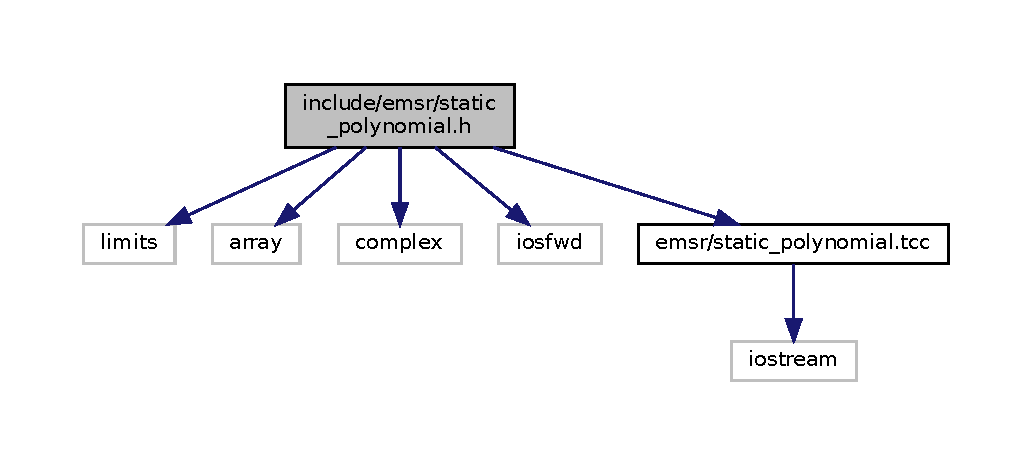
\includegraphics[width=350pt]{static__polynomial_8h__incl}
\end{center}
\end{figure}
\subsection*{Classes}
\begin{DoxyCompactItemize}
\item 
struct \hyperlink{struct____gnu__cxx_1_1____divmod__t}{\+\_\+\+\_\+gnu\+\_\+cxx\+::\+\_\+\+\_\+divmod\+\_\+t$<$ \+\_\+\+Tp, \+\_\+\+Size\+N, \+\_\+\+Size\+D $>$}
\item 
class \hyperlink{class____gnu__cxx_1_1__StaticPolynomial}{\+\_\+\+\_\+gnu\+\_\+cxx\+::\+\_\+\+Static\+Polynomial$<$ \+\_\+\+Tp, \+\_\+\+Size $>$}
\end{DoxyCompactItemize}
\subsection*{Namespaces}
\begin{DoxyCompactItemize}
\item 
 \hyperlink{namespace____gnu__cxx}{\+\_\+\+\_\+gnu\+\_\+cxx}
\end{DoxyCompactItemize}
\subsection*{Functions}
\begin{DoxyCompactItemize}
\item 
{\footnotesize template$<$typename \+\_\+\+Tp , std\+::size\+\_\+t \+\_\+\+SizeN, std\+::size\+\_\+t \+\_\+\+SizeD$>$ }\\constexpr \+\_\+\+\_\+divmod\+\_\+t$<$ \+\_\+\+Tp, \+\_\+\+SizeN, \+\_\+\+SizeD $>$ \hyperlink{namespace____gnu__cxx_a33c585ec7ce2ac87e7f5cb1b1fe403b1}{\+\_\+\+\_\+gnu\+\_\+cxx\+::divmod} (const \+\_\+\+Static\+Polynomial$<$ \+\_\+\+Tp, \+\_\+\+SizeN $>$ \&\+\_\+\+\_\+num, const \+\_\+\+Static\+Polynomial$<$ \+\_\+\+Tp, \+\_\+\+SizeD $>$ \&\+\_\+\+\_\+den)
\item 
{\footnotesize template$<$typename \+\_\+\+Tp , std\+::size\+\_\+t \+\_\+\+SizeA, std\+::size\+\_\+t \+\_\+\+SizeB$>$ }\\constexpr bool \hyperlink{namespace____gnu__cxx_af19ad85b9b29562d2e134f3db6b3a651}{\+\_\+\+\_\+gnu\+\_\+cxx\+::operator!=} (const \+\_\+\+Static\+Polynomial$<$ \+\_\+\+Tp, \+\_\+\+SizeA $>$ \&\+\_\+\+\_\+pa, const \+\_\+\+Static\+Polynomial$<$ \+\_\+\+Tp, \+\_\+\+SizeB $>$ \&\+\_\+\+\_\+pb)
\item 
{\footnotesize template$<$typename \+\_\+\+Tp , std\+::size\+\_\+t \+\_\+\+Size$>$ }\\constexpr bool \hyperlink{namespace____gnu__cxx_ac759e59bd5e23de4cbd603b846081718}{\+\_\+\+\_\+gnu\+\_\+cxx\+::operator!=} (const \+\_\+\+Static\+Polynomial$<$ \+\_\+\+Tp, \+\_\+\+Size $>$ \&\+\_\+\+\_\+pa, const \+\_\+\+Static\+Polynomial$<$ \+\_\+\+Tp, \+\_\+\+Size $>$ \&\+\_\+\+\_\+pb)
\item 
{\footnotesize template$<$typename \+\_\+\+Tp , std\+::size\+\_\+t \+\_\+\+SizeP, std\+::size\+\_\+t \+\_\+\+SizeQ$>$ }\\constexpr \+\_\+\+Static\+Polynomial$<$ \+\_\+\+Tp, \+\_\+\+\_\+divmod\+\_\+t$<$ \+\_\+\+Tp, \+\_\+\+SizeP, \+\_\+\+SizeQ $>$\+::\+\_\+\+Size\+Rem $>$ \hyperlink{namespace____gnu__cxx_a15445a05944d0b0235051dbfb380f9bf}{\+\_\+\+\_\+gnu\+\_\+cxx\+::operator\%} (const \+\_\+\+Static\+Polynomial$<$ \+\_\+\+Tp, \+\_\+\+SizeP $>$ \&\+\_\+P, const \+\_\+\+Static\+Polynomial$<$ \+\_\+\+Tp, \+\_\+\+SizeQ $>$ \&\+\_\+Q)
\item 
{\footnotesize template$<$typename \+\_\+\+Tp , std\+::size\+\_\+t \+\_\+\+Size$>$ }\\constexpr \+\_\+\+Static\+Polynomial$<$ \+\_\+\+Tp, \+\_\+\+Size $>$ \hyperlink{namespace____gnu__cxx_a71781c23f8dd75f9cf9d7610a26225ad}{\+\_\+\+\_\+gnu\+\_\+cxx\+::operator$\ast$} (const \+\_\+\+Static\+Polynomial$<$ \+\_\+\+Tp, \+\_\+\+Size $>$ \&\+\_\+\+\_\+poly, const \+\_\+\+Tp \&\+\_\+\+\_\+x)
\item 
{\footnotesize template$<$typename \+\_\+\+Tp , std\+::size\+\_\+t \+\_\+\+Size$>$ }\\\+\_\+\+Static\+Polynomial$<$ \+\_\+\+Tp, \+\_\+\+Size $>$ \hyperlink{namespace____gnu__cxx_a91cea4290bb3218fc6d869a655db5891}{\+\_\+\+\_\+gnu\+\_\+cxx\+::operator$\ast$} (const \+\_\+\+Tp \&\+\_\+\+\_\+x, const \+\_\+\+Static\+Polynomial$<$ \+\_\+\+Tp, \+\_\+\+Size $>$ \&\+\_\+\+\_\+poly)
\item 
{\footnotesize template$<$typename \+\_\+\+Tp , std\+::size\+\_\+t \+\_\+\+SizeP, std\+::size\+\_\+t \+\_\+\+SizeQ$>$ }\\constexpr \+\_\+\+Static\+Polynomial$<$ \+\_\+\+Tp, \+\_\+\+SizeP+\+\_\+\+SizeQ -\/ 1 $>$ \hyperlink{namespace____gnu__cxx_a8570f2d82260e7f64d985be3ddf007f8}{\+\_\+\+\_\+gnu\+\_\+cxx\+::operator$\ast$} (const \+\_\+\+Static\+Polynomial$<$ \+\_\+\+Tp, \+\_\+\+SizeP $>$ \&\+\_\+P, const \+\_\+\+Static\+Polynomial$<$ \+\_\+\+Tp, \+\_\+\+SizeQ $>$ \&\+\_\+Q)
\item 
{\footnotesize template$<$typename \+\_\+\+Tp , std\+::size\+\_\+t \+\_\+\+Size$>$ }\\constexpr \+\_\+\+Static\+Polynomial$<$ \+\_\+\+Tp, \+\_\+\+Size $>$ \hyperlink{namespace____gnu__cxx_a6864af2e99c7797a84209d8dffcf11e5}{\+\_\+\+\_\+gnu\+\_\+cxx\+::operator+} (const \+\_\+\+Static\+Polynomial$<$ \+\_\+\+Tp, \+\_\+\+Size $>$ \&\+\_\+\+\_\+poly, const \+\_\+\+Tp \&\+\_\+\+\_\+x)
\item 
{\footnotesize template$<$typename \+\_\+\+Tp , std\+::size\+\_\+t \+\_\+\+Size$>$ }\\\+\_\+\+Static\+Polynomial$<$ \+\_\+\+Tp, \+\_\+\+Size $>$ \hyperlink{namespace____gnu__cxx_a06334b50d2c25cdadf11c1785a57cde0}{\+\_\+\+\_\+gnu\+\_\+cxx\+::operator+} (const \+\_\+\+Tp \&\+\_\+\+\_\+x, const \+\_\+\+Static\+Polynomial$<$ \+\_\+\+Tp, \+\_\+\+Size $>$ \&\+\_\+\+\_\+poly)
\item 
{\footnotesize template$<$typename \+\_\+\+Tp , std\+::size\+\_\+t \+\_\+\+SizeP, std\+::size\+\_\+t \+\_\+\+SizeQ$>$ }\\constexpr \+\_\+\+Static\+Polynomial$<$ \+\_\+\+Tp, std\+::max(\+\_\+\+SizeP, \+\_\+\+SizeQ)$>$ \hyperlink{namespace____gnu__cxx_ab21b8f613598d3de78239f9a5d45bee7}{\+\_\+\+\_\+gnu\+\_\+cxx\+::operator+} (const \+\_\+\+Static\+Polynomial$<$ \+\_\+\+Tp, \+\_\+\+SizeP $>$ \&\+\_\+P, const \+\_\+\+Static\+Polynomial$<$ \+\_\+\+Tp, \+\_\+\+SizeQ $>$ \&\+\_\+Q)
\item 
{\footnotesize template$<$typename \+\_\+\+Tp , std\+::size\+\_\+t \+\_\+\+Size$>$ }\\constexpr \+\_\+\+Static\+Polynomial$<$ \+\_\+\+Tp, \+\_\+\+Size $>$ \hyperlink{namespace____gnu__cxx_a9f3b5d6e3db0c359eb0c8c067fc9ae05}{\+\_\+\+\_\+gnu\+\_\+cxx\+::operator-\/} (const \+\_\+\+Static\+Polynomial$<$ \+\_\+\+Tp, \+\_\+\+Size $>$ \&\+\_\+\+\_\+poly, const \+\_\+\+Tp \&\+\_\+\+\_\+x)
\item 
{\footnotesize template$<$typename \+\_\+\+Tp , std\+::size\+\_\+t \+\_\+\+Size$>$ }\\\+\_\+\+Static\+Polynomial$<$ \+\_\+\+Tp, \+\_\+\+Size $>$ \hyperlink{namespace____gnu__cxx_a6bc4eecdfefce0b2dea328cb6cc5412a}{\+\_\+\+\_\+gnu\+\_\+cxx\+::operator-\/} (const \+\_\+\+Tp \&\+\_\+\+\_\+x, const \+\_\+\+Static\+Polynomial$<$ \+\_\+\+Tp, \+\_\+\+Size $>$ \&\+\_\+\+\_\+poly)
\item 
{\footnotesize template$<$typename \+\_\+\+Tp , std\+::size\+\_\+t \+\_\+\+SizeP, std\+::size\+\_\+t \+\_\+\+SizeQ$>$ }\\constexpr \+\_\+\+Static\+Polynomial$<$ \+\_\+\+Tp, std\+::max(\+\_\+\+SizeP, \+\_\+\+SizeQ)$>$ \hyperlink{namespace____gnu__cxx_a7a0dd6f28607ef9be1e5eb053716076f}{\+\_\+\+\_\+gnu\+\_\+cxx\+::operator-\/} (const \+\_\+\+Static\+Polynomial$<$ \+\_\+\+Tp, \+\_\+\+SizeP $>$ \&\+\_\+P, const \+\_\+\+Static\+Polynomial$<$ \+\_\+\+Tp, \+\_\+\+SizeQ $>$ \&\+\_\+Q)
\item 
{\footnotesize template$<$typename \+\_\+\+Tp , std\+::size\+\_\+t \+\_\+\+Size$>$ }\\constexpr \+\_\+\+Static\+Polynomial$<$ \+\_\+\+Tp, \+\_\+\+Size $>$ \hyperlink{namespace____gnu__cxx_a646b9470b937733c916192c121e8ecdb}{\+\_\+\+\_\+gnu\+\_\+cxx\+::operator/} (const \+\_\+\+Static\+Polynomial$<$ \+\_\+\+Tp, \+\_\+\+Size $>$ \&\+\_\+\+\_\+poly, const \+\_\+\+Tp \&\+\_\+\+\_\+x)
\item 
{\footnotesize template$<$typename \+\_\+\+Tp , std\+::size\+\_\+t \+\_\+\+SizeP, std\+::size\+\_\+t \+\_\+\+SizeQ$>$ }\\constexpr \+\_\+\+Static\+Polynomial$<$ \+\_\+\+Tp, \+\_\+\+\_\+divmod\+\_\+t$<$ \+\_\+\+Tp, \+\_\+\+SizeP, \+\_\+\+SizeQ $>$\+::\+\_\+\+Size\+Quo $>$ \hyperlink{namespace____gnu__cxx_a451a609c6de284cdeed747a994938801}{\+\_\+\+\_\+gnu\+\_\+cxx\+::operator/} (const \+\_\+\+Static\+Polynomial$<$ \+\_\+\+Tp, \+\_\+\+SizeP $>$ \&\+\_\+P, const \+\_\+\+Static\+Polynomial$<$ \+\_\+\+Tp, \+\_\+\+SizeQ $>$ \&\+\_\+Q)
\item 
{\footnotesize template$<$typename CharT , typename Traits , typename \+\_\+\+Tp , std\+::size\+\_\+t \+\_\+\+Size$>$ }\\std\+::basic\+\_\+ostream$<$ CharT, Traits $>$ \& \hyperlink{namespace____gnu__cxx_a143c7d2302fc613fd818f9149707b753}{\+\_\+\+\_\+gnu\+\_\+cxx\+::operator$<$$<$} (std\+::basic\+\_\+ostream$<$ CharT, Traits $>$ \&\+\_\+\+\_\+os, const \+\_\+\+Static\+Polynomial$<$ \+\_\+\+Tp, \+\_\+\+Size $>$ \&\+\_\+\+\_\+poly)
\item 
{\footnotesize template$<$typename \+\_\+\+Tp , std\+::size\+\_\+t \+\_\+\+SizeA, std\+::size\+\_\+t \+\_\+\+SizeB$>$ }\\constexpr bool \hyperlink{namespace____gnu__cxx_a316d841c3d2addecec46960379815cd4}{\+\_\+\+\_\+gnu\+\_\+cxx\+::operator==} (const \+\_\+\+Static\+Polynomial$<$ \+\_\+\+Tp, \+\_\+\+SizeA $>$ \&, const \+\_\+\+Static\+Polynomial$<$ \+\_\+\+Tp, \+\_\+\+SizeB $>$ \&)
\item 
{\footnotesize template$<$typename \+\_\+\+Tp , std\+::size\+\_\+t \+\_\+\+Size$>$ }\\constexpr bool \hyperlink{namespace____gnu__cxx_a4156deb610ec73be9e2f56a1a4caf391}{\+\_\+\+\_\+gnu\+\_\+cxx\+::operator==} (const \+\_\+\+Static\+Polynomial$<$ \+\_\+\+Tp, \+\_\+\+Size $>$ \&\+\_\+\+\_\+pa, const \+\_\+\+Static\+Polynomial$<$ \+\_\+\+Tp, \+\_\+\+Size $>$ \&\+\_\+\+\_\+pb)
\end{DoxyCompactItemize}


\subsection{Detailed Description}
Class definition for a static polynomial. 
%--- End generated contents ---

% Index
\backmatter
\newpage
\phantomsection
\clearemptydoublepage
\addcontentsline{toc}{chapter}{Index}
\printindex

\end{document}
